\documentclass[12pt,english]{article}

\usepackage[a4paper,
            bindingoffset=0.2in,
            left=1in,
            right=1in,
            top=1in,
            bottom=1in,
            footskip=.25in]{geometry}

% % Set page size and margins
% % Replace `letterpaper' with`a4paper' for UK/EU standard size
% \usepackage[letterpaper,top=2cm,bottom=2cm,left=3cm,right=3cm,marginparwidth=1.75cm]{geometry}
\topmargin=-.3in \oddsidemargin=.3in \evensidemargin=.3in \textheight=9in \textwidth=6in

\usepackage{tikz}
\usepackage{pgfplots}
\usepackage{float}
\usepackage{adjustbox}
\usepackage{multirow}
\usepackage{hhline}

\usepackage{algorithm, algpseudocode}
\usepackage{setspace}

\algrenewcommand\textproc{}

\algnewcommand\algorithmicswitch{\textbf{switch}}
\algnewcommand\algorithmiccase{\textbf{case}}
\algnewcommand\algorithmicassert{\texttt{assert}}
\algnewcommand\Assert[1]{\State \algorithmicassert(#1)}%
% New "environments"
\algdef{SE}[SWITCH]{Switch}{EndSwitch}[1]{\algorithmicswitch\ #1\ \algorithmicdo}{\algorithmicend\ \algorithmicswitch}%
\algdef{SE}[CASE]{Case}{EndCase}[1]{\algorithmiccase\ #1}{\algorithmicend\ \algorithmiccase}%
\newcommand{\pluseq}{\mathrel{{+}{=}}}
\algblockdefx[Foreach]{Foreach}{EndForeach}[1]{\textbf{foreach} #1 \textbf{do}}{\textbf{end foreach}}


% \newcommand{\makeheight}[1]{%
%   \settoheight{\dimen0}{T}% a capital letter
%   \rule[-\dimexpr(#1-\dimen0)/2]{0pt}{#1}%
% }

\newcommand{\myindent}[1]{
\newline\makebox[#1cm]{}
}

\usepackage{amsmath}

\usepackage{authblk}

% \usepackage{tabularx, booktabs}


\title{\textbf{Inner vs. Inter City Transmission in the Hadith Social Network}}

\author[1]{Danny Halawi\thanks{dannyhalawi15@gmail.com}}
\author[2]{Mairaj Syed\thanks{msyed@ucdavis.edu}}
\affil[1]{Department of Computer Science, University of California, Berkeley}
\affil[2]{Department of Religious Studies, University of California, Davis}


\date{}
\begin{document}
\maketitle

\newpage

% \newcolumntype{U}{>{\centering\arraybackslash}p{2cm}}
% \newcolumntype{V}{>{\centering\arraybackslash}p{1.75cm}}
% \newcolumntype{W}{>{\centering\arraybackslash}p{2cm}}
% \newcolumntype{E}{>{\centering\arraybackslash}p{1.5cm}}

\section{Hadith to Edges}
\vspace*{-0.4cm}
\hspace*{-2cm}
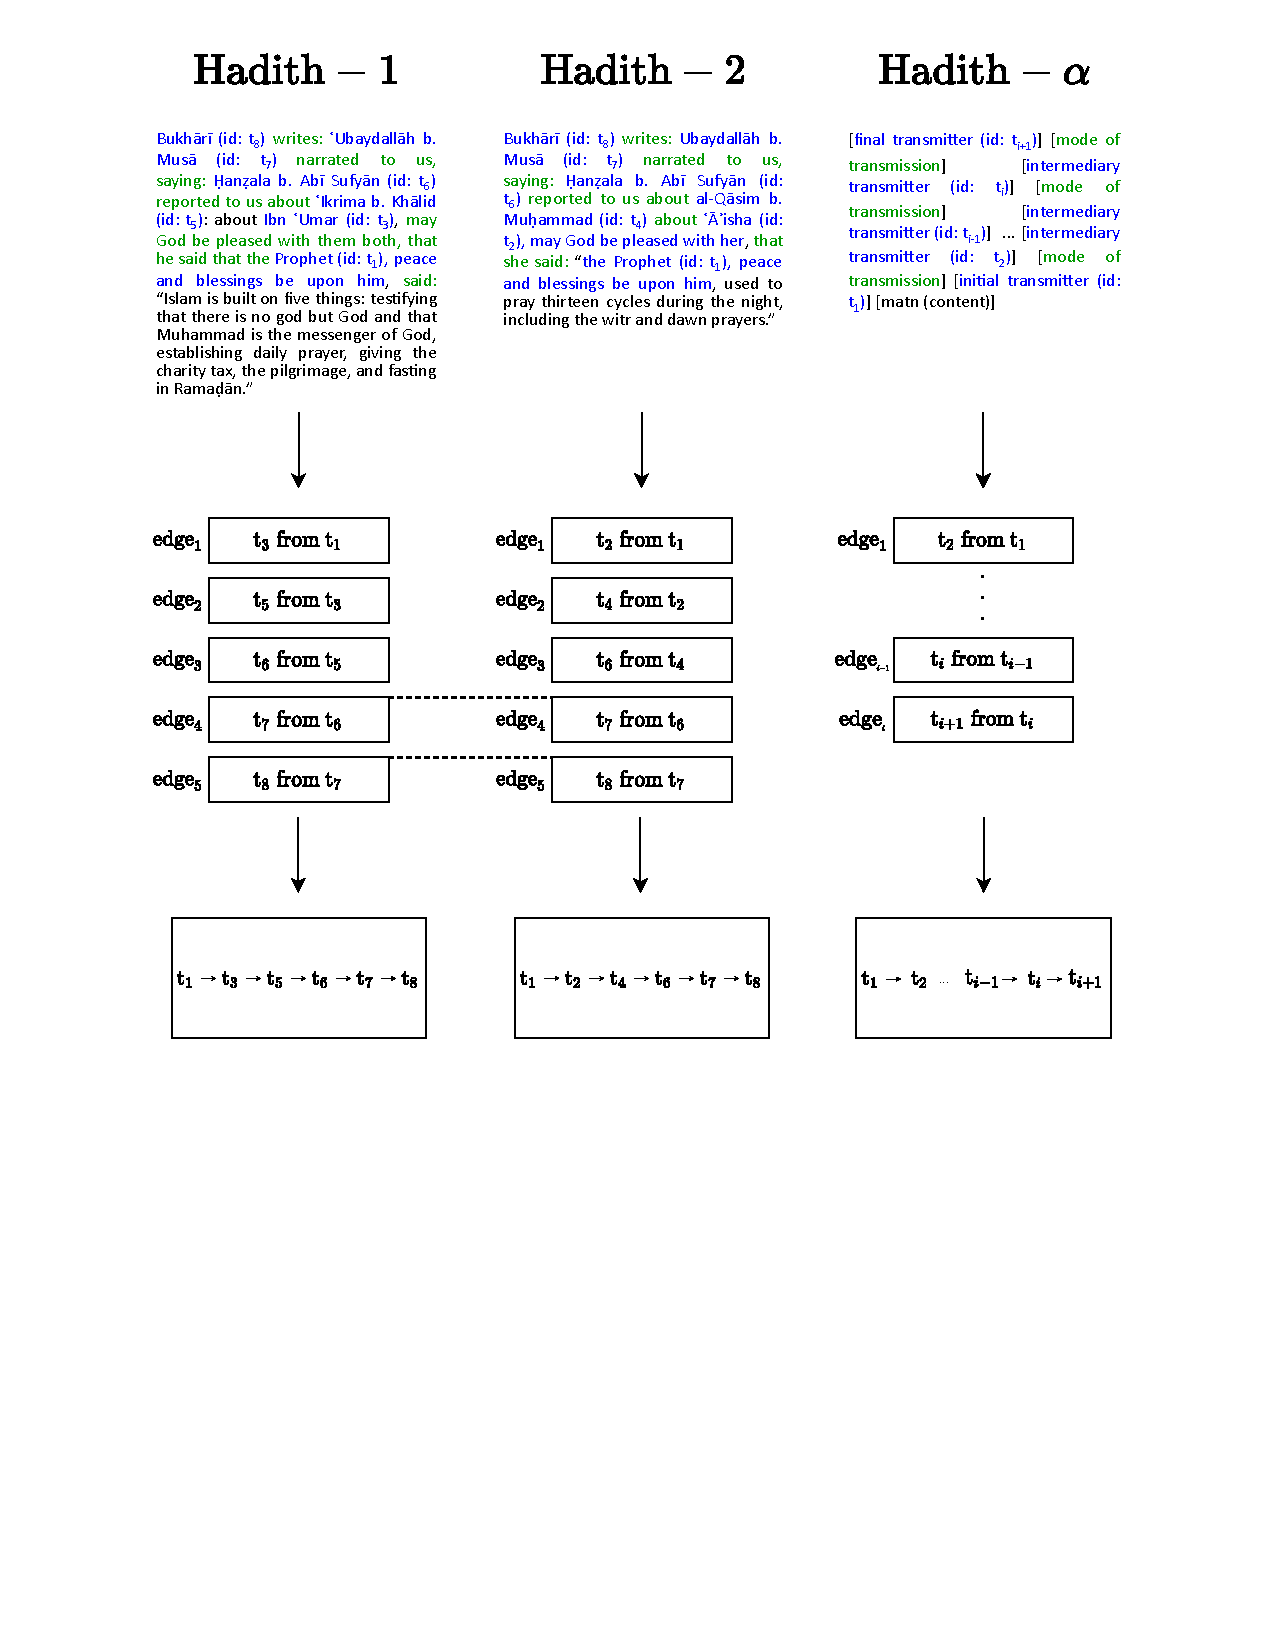
\includegraphics[scale=0.9]{hadith-to-edges/b0_hadith_to_edges.pdf}

\newpage
\section{Edges to HSN}
\vspace*{-0.4cm}
\hspace*{-2cm}
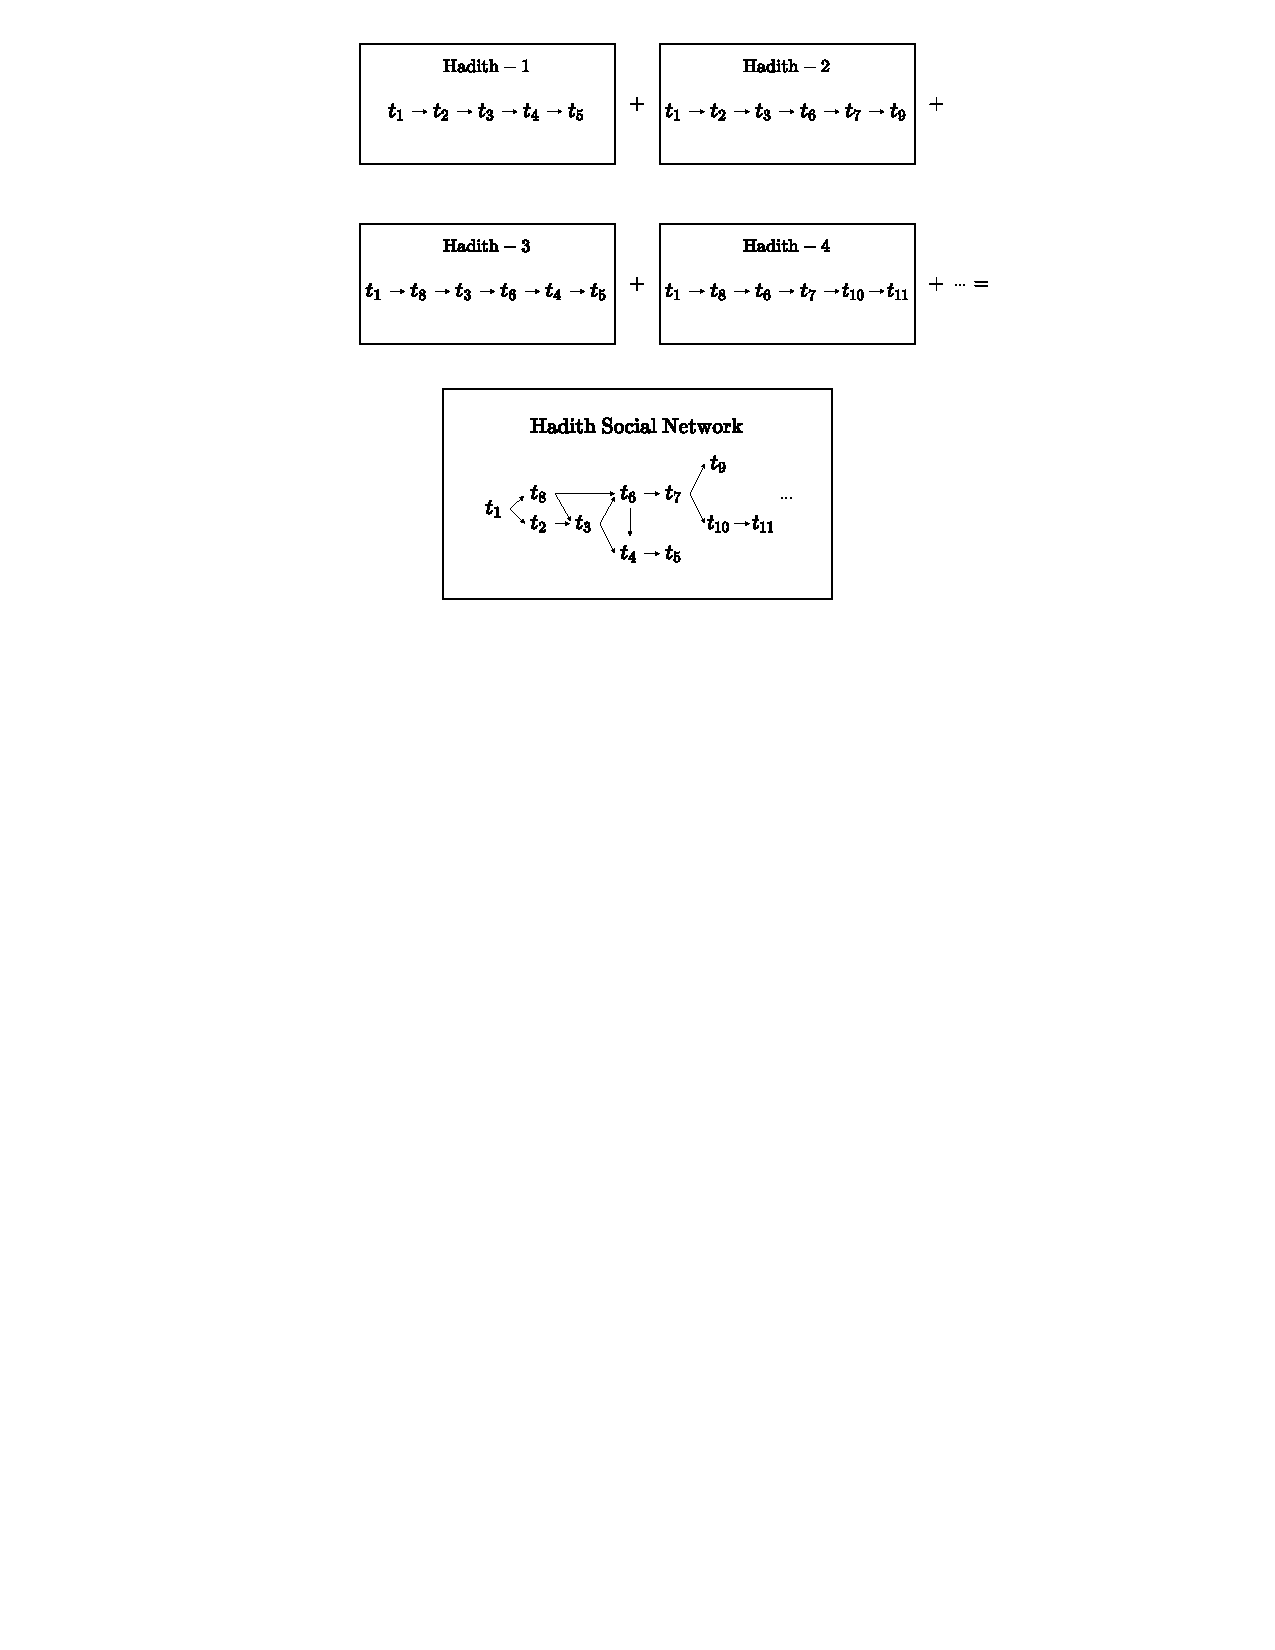
\includegraphics[scale=0.9]{edges-to-hsn/b1_edges_to_hsn.pdf}

\newpage
\section{Edges to City Network}
\vspace*{-0.4cm}
\hspace*{-2cm}
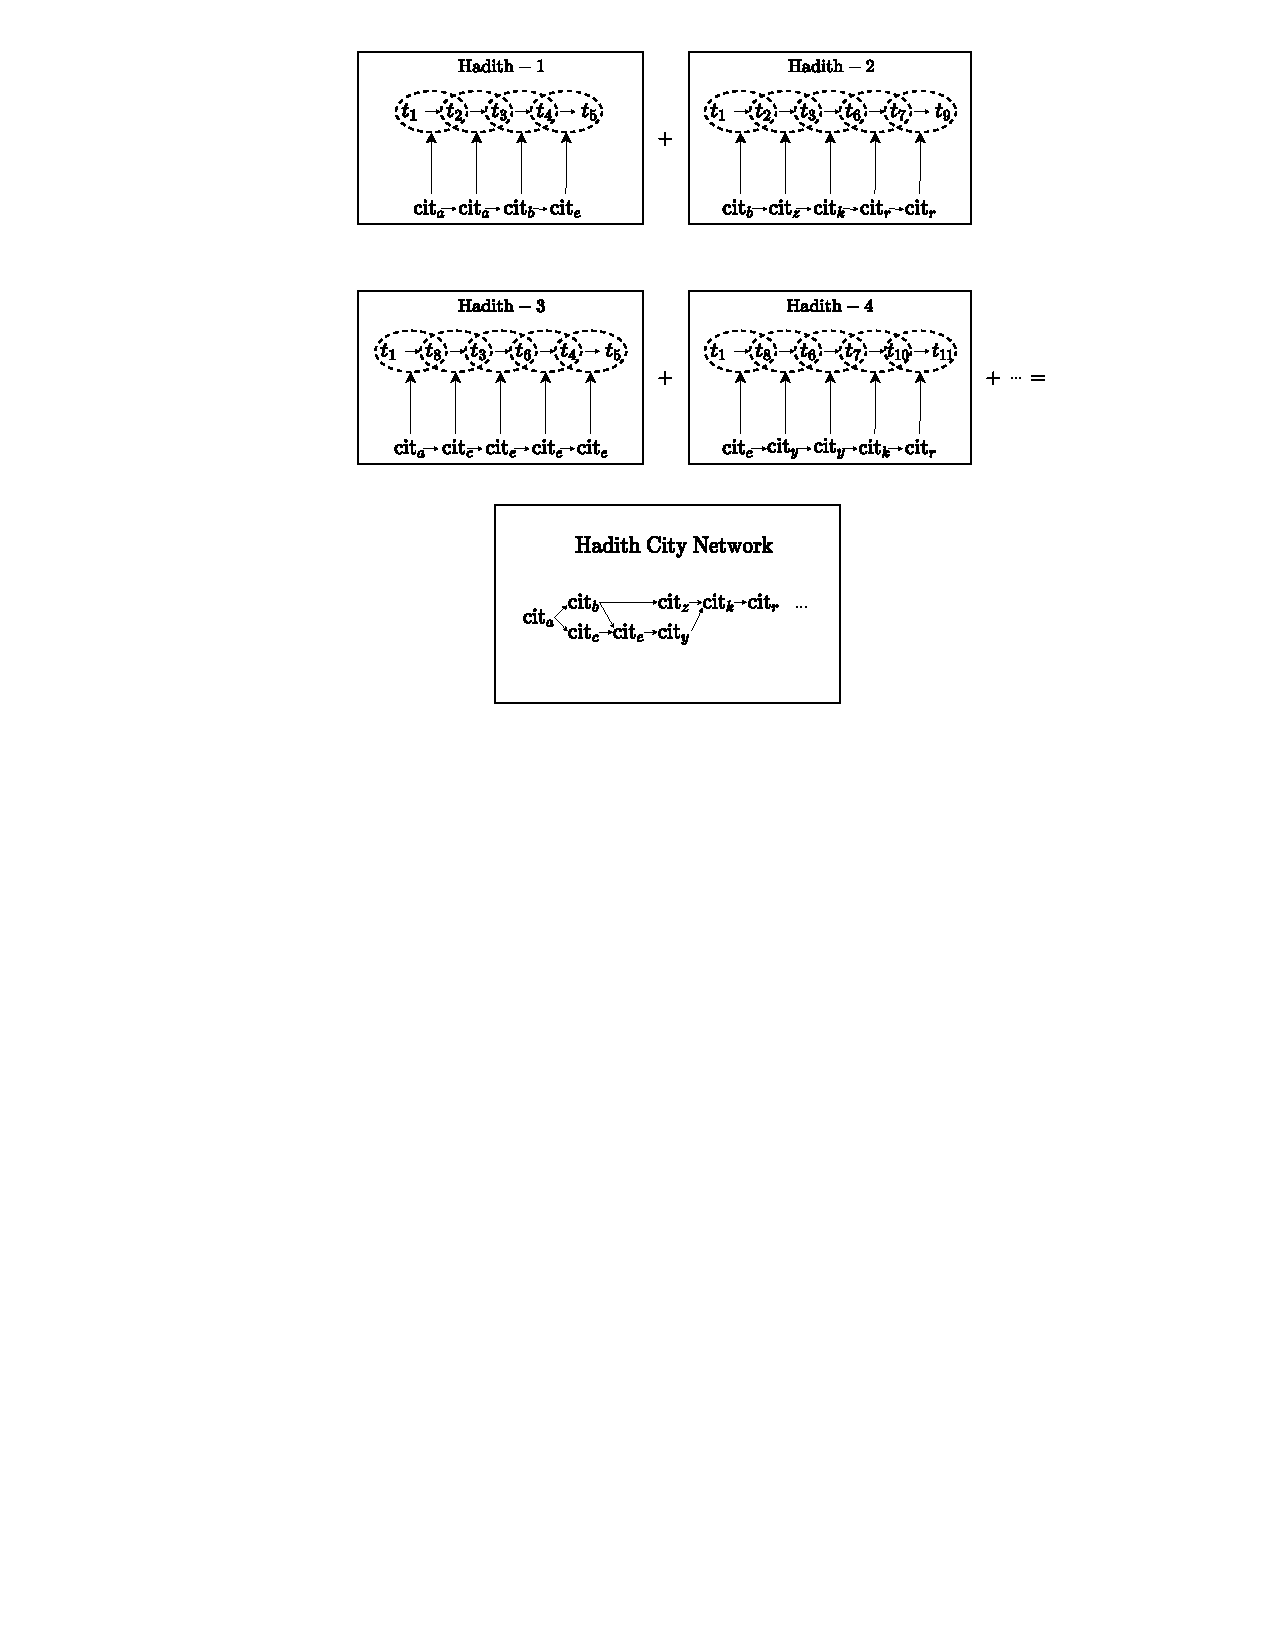
\includegraphics[scale=0.9]{edges-to-city-network/b2_edges_to_city_network.pdf}

\section{Bird's-eye View First 350 Years}
\begin{center}
\begin{tikzpicture}[scale=.95]
\begin{axis}[
    xmin = 0, xmax = 360,
    ymin = 0, ymax = 1,
    xtick distance = 20,
    ytick distance = 0.10,
    minor tick num = 3,
    major grid style = {lightgray},
    minor grid style = {lightgray!25},
    width = \textwidth,
    height = 0.75\textwidth,
    legend cell align = {left},
    legend pos = north west,
    axis lines = left
]
\addplot[black, mark = 10-pointed star, mark options={fill=white}, thick] table [x=year, y=ratio, col sep=comma] {a1_inner_transmission_over_total_transmission_5_year_buckets_350_years.csv};
\addplot[black, mark = Mercedes star, mark options={fill=white}, thick] table [x=year, y=ratio, col sep=comma] {a1_inter_transmission_over_total_transmission_5_year_buckets_350_years.csv};

\begin{scope}
	\draw (250,20) -- 
		plot[mark=10-pointed star, mark options={fill=white}] (260,20) -- (270,20) 
		node[right]{inner-city};
	\draw (250,15) -- 
		plot[mark=Mercedes star, mark options={fill=white}] (260,15) -- (270,15) 
		node[right]{inter-city};
	\draw[red, dashed] (0+11,50) -- 
		 (362,50);
\end{scope}

% \legend{
%     inner-city to inter-city,
%     inter-city to inner-city
% }
\end{axis}
\end{tikzpicture}
\end{center}

\newpage
\section{Bird's-eye View First 600 Years}

\begin{center}
\begin{tikzpicture}[scale=.95]
\begin{axis}[
    xmin = 0, xmax = 630,
    ymin = 0, ymax = 1,
    xtick distance = 40,
    ytick distance = 0.10,
    minor tick num = 6,
    major grid style = {lightgray},
    minor grid style = {lightgray!25},
    width = \textwidth,
    height = 0.75\textwidth,
    legend cell align = {left},
    legend pos = north west,
    axis lines = left
]
\addplot[black, mark = 10-pointed star, mark options={fill=white}, thick] table [x=year, y=ratio, col sep=comma] {a1_inner_transmission_over_total_transmission_5_year_buckets_600_years.csv};
\addplot[black, mark = Mercedes star, mark options={fill=white}, thick] table [x=year, y=ratio, col sep=comma] {a1_inter_transmission_over_total_transmission_5_year_buckets_600_years.csv};

\begin{scope}
	\draw (430,15) -- 
		plot[mark=10-pointed star, mark options={fill=white}] (440,15) -- (450,15) 
		node[right]{inner-city};
	\draw (430,10) -- 
		plot[mark=Mercedes star, mark options={fill=white}] (440,10) -- (450,10) 
		node[right]{inter-city};
	\draw[red, dashed] (0+11,50) -- 
		 (615,50);
\end{scope}

% \legend{
%     inner-city to inter-city,
%     inter-city to inner-city
% }
\end{axis}
\end{tikzpicture}
\end{center}

\newpage
\section{City Analysis}
\begin{center}
\vspace*{-1cm}
    %% Creator: Matplotlib, PGF backend
%%
%% To include the figure in your LaTeX document, write
%%   \input{<filename>.pgf}
%%
%% Make sure the required packages are loaded in your preamble
%%   \usepackage{pgf}
%%
%% and, on pdftex
%%   \usepackage[utf8]{inputenc}\DeclareUnicodeCharacter{2212}{-}
%%
%% or, on luatex and xetex
%%   \usepackage{unicode-math}
%%
%% Figures using additional raster images can only be included by \input if
%% they are in the same directory as the main LaTeX file. For loading figures
%% from other directories you can use the `import` package
%%   \usepackage{import}
%%
%% and then include the figures with
%%   \import{<path to file>}{<filename>.pgf}
%%
%% Matplotlib used the following preamble
%%
\begingroup%
\makeatletter%
\begin{pgfpicture}%
\pgfpathrectangle{\pgfpointorigin}{\pgfqpoint{6.000000in}{4.000000in}}%
\pgfusepath{use as bounding box, clip}%
\begin{pgfscope}%
\pgfsetbuttcap%
\pgfsetmiterjoin%
\pgfsetlinewidth{0.000000pt}%
\definecolor{currentstroke}{rgb}{1.000000,1.000000,1.000000}%
\pgfsetstrokecolor{currentstroke}%
\pgfsetstrokeopacity{0.000000}%
\pgfsetdash{}{0pt}%
\pgfpathmoveto{\pgfqpoint{0.000000in}{0.000000in}}%
\pgfpathlineto{\pgfqpoint{6.000000in}{0.000000in}}%
\pgfpathlineto{\pgfqpoint{6.000000in}{4.000000in}}%
\pgfpathlineto{\pgfqpoint{0.000000in}{4.000000in}}%
\pgfpathclose%
\pgfusepath{}%
\end{pgfscope}%
\begin{pgfscope}%
\pgfsetbuttcap%
\pgfsetmiterjoin%
\definecolor{currentfill}{rgb}{0.501961,0.501961,0.501961}%
\pgfsetfillcolor{currentfill}%
\pgfsetlinewidth{0.000000pt}%
\definecolor{currentstroke}{rgb}{0.000000,0.000000,0.000000}%
\pgfsetstrokecolor{currentstroke}%
\pgfsetstrokeopacity{0.000000}%
\pgfsetdash{}{0pt}%
\pgfpathmoveto{\pgfqpoint{0.863936in}{0.500000in}}%
\pgfpathlineto{\pgfqpoint{5.286064in}{0.500000in}}%
\pgfpathlineto{\pgfqpoint{5.286064in}{3.520000in}}%
\pgfpathlineto{\pgfqpoint{0.863936in}{3.520000in}}%
\pgfpathclose%
\pgfusepath{fill}%
\end{pgfscope}%
\begin{pgfscope}%
\pgfpathrectangle{\pgfqpoint{0.863936in}{0.500000in}}{\pgfqpoint{4.422128in}{3.020000in}}%
\pgfusepath{clip}%
\pgfsetbuttcap%
\pgfsetmiterjoin%
\definecolor{currentfill}{rgb}{0.000000,0.000000,0.000000}%
\pgfsetfillcolor{currentfill}%
\pgfsetlinewidth{1.003750pt}%
\definecolor{currentstroke}{rgb}{0.000000,0.000000,0.000000}%
\pgfsetstrokecolor{currentstroke}%
\pgfsetdash{}{0pt}%
\pgfpathmoveto{\pgfqpoint{1.090280in}{3.357924in}}%
\pgfpathlineto{\pgfqpoint{1.121508in}{3.357924in}}%
\pgfpathlineto{\pgfqpoint{1.121508in}{3.326696in}}%
\pgfpathlineto{\pgfqpoint{1.090280in}{3.326696in}}%
\pgfpathclose%
\pgfusepath{stroke,fill}%
\end{pgfscope}%
\begin{pgfscope}%
\pgfpathrectangle{\pgfqpoint{0.863936in}{0.500000in}}{\pgfqpoint{4.422128in}{3.020000in}}%
\pgfusepath{clip}%
\pgfsetbuttcap%
\pgfsetmiterjoin%
\definecolor{currentfill}{rgb}{0.000000,0.000000,1.000000}%
\pgfsetfillcolor{currentfill}%
\pgfsetlinewidth{1.003750pt}%
\definecolor{currentstroke}{rgb}{0.000000,0.000000,1.000000}%
\pgfsetstrokecolor{currentstroke}%
\pgfsetdash{}{0pt}%
\pgfpathmoveto{\pgfqpoint{1.064942in}{3.267432in}}%
\pgfpathlineto{\pgfqpoint{1.146846in}{3.267432in}}%
\pgfpathlineto{\pgfqpoint{1.146846in}{3.185528in}}%
\pgfpathlineto{\pgfqpoint{1.064942in}{3.185528in}}%
\pgfpathclose%
\pgfusepath{stroke,fill}%
\end{pgfscope}%
\begin{pgfscope}%
\pgfpathrectangle{\pgfqpoint{0.863936in}{0.500000in}}{\pgfqpoint{4.422128in}{3.020000in}}%
\pgfusepath{clip}%
\pgfsetbuttcap%
\pgfsetmiterjoin%
\definecolor{currentfill}{rgb}{1.000000,1.000000,1.000000}%
\pgfsetfillcolor{currentfill}%
\pgfsetlinewidth{1.003750pt}%
\definecolor{currentstroke}{rgb}{1.000000,1.000000,1.000000}%
\pgfsetstrokecolor{currentstroke}%
\pgfsetdash{}{0pt}%
\pgfpathmoveto{\pgfqpoint{1.101908in}{3.114636in}}%
\pgfpathlineto{\pgfqpoint{1.109879in}{3.114636in}}%
\pgfpathlineto{\pgfqpoint{1.109879in}{3.106665in}}%
\pgfpathlineto{\pgfqpoint{1.101908in}{3.106665in}}%
\pgfpathclose%
\pgfusepath{stroke,fill}%
\end{pgfscope}%
\begin{pgfscope}%
\pgfpathrectangle{\pgfqpoint{0.863936in}{0.500000in}}{\pgfqpoint{4.422128in}{3.020000in}}%
\pgfusepath{clip}%
\pgfsetbuttcap%
\pgfsetmiterjoin%
\definecolor{currentfill}{rgb}{1.000000,1.000000,1.000000}%
\pgfsetfillcolor{currentfill}%
\pgfsetlinewidth{1.003750pt}%
\definecolor{currentstroke}{rgb}{1.000000,1.000000,1.000000}%
\pgfsetstrokecolor{currentstroke}%
\pgfsetdash{}{0pt}%
\pgfpathmoveto{\pgfqpoint{1.084555in}{3.016159in}}%
\pgfpathlineto{\pgfqpoint{1.127233in}{3.016159in}}%
\pgfpathlineto{\pgfqpoint{1.127233in}{2.973482in}}%
\pgfpathlineto{\pgfqpoint{1.084555in}{2.973482in}}%
\pgfpathclose%
\pgfusepath{stroke,fill}%
\end{pgfscope}%
\begin{pgfscope}%
\pgfpathrectangle{\pgfqpoint{0.863936in}{0.500000in}}{\pgfqpoint{4.422128in}{3.020000in}}%
\pgfusepath{clip}%
\pgfsetbuttcap%
\pgfsetmiterjoin%
\definecolor{currentfill}{rgb}{1.000000,1.000000,1.000000}%
\pgfsetfillcolor{currentfill}%
\pgfsetlinewidth{1.003750pt}%
\definecolor{currentstroke}{rgb}{1.000000,1.000000,1.000000}%
\pgfsetstrokecolor{currentstroke}%
\pgfsetdash{}{0pt}%
\pgfpathmoveto{\pgfqpoint{1.073418in}{2.911467in}}%
\pgfpathlineto{\pgfqpoint{1.138370in}{2.911467in}}%
\pgfpathlineto{\pgfqpoint{1.138370in}{2.846515in}}%
\pgfpathlineto{\pgfqpoint{1.073418in}{2.846515in}}%
\pgfpathclose%
\pgfusepath{stroke,fill}%
\end{pgfscope}%
\begin{pgfscope}%
\pgfpathrectangle{\pgfqpoint{0.863936in}{0.500000in}}{\pgfqpoint{4.422128in}{3.020000in}}%
\pgfusepath{clip}%
\pgfsetbuttcap%
\pgfsetmiterjoin%
\definecolor{currentfill}{rgb}{0.000000,0.000000,0.000000}%
\pgfsetfillcolor{currentfill}%
\pgfsetlinewidth{1.003750pt}%
\definecolor{currentstroke}{rgb}{0.000000,0.000000,0.000000}%
\pgfsetstrokecolor{currentstroke}%
\pgfsetdash{}{0pt}%
\pgfpathmoveto{\pgfqpoint{1.088688in}{2.780366in}}%
\pgfpathlineto{\pgfqpoint{1.123099in}{2.780366in}}%
\pgfpathlineto{\pgfqpoint{1.123099in}{2.745955in}}%
\pgfpathlineto{\pgfqpoint{1.088688in}{2.745955in}}%
\pgfpathclose%
\pgfusepath{stroke,fill}%
\end{pgfscope}%
\begin{pgfscope}%
\pgfpathrectangle{\pgfqpoint{0.863936in}{0.500000in}}{\pgfqpoint{4.422128in}{3.020000in}}%
\pgfusepath{clip}%
\pgfsetbuttcap%
\pgfsetmiterjoin%
\definecolor{currentfill}{rgb}{0.000000,0.000000,1.000000}%
\pgfsetfillcolor{currentfill}%
\pgfsetlinewidth{1.003750pt}%
\definecolor{currentstroke}{rgb}{0.000000,0.000000,1.000000}%
\pgfsetstrokecolor{currentstroke}%
\pgfsetdash{}{0pt}%
\pgfpathmoveto{\pgfqpoint{1.064942in}{2.688283in}}%
\pgfpathlineto{\pgfqpoint{1.146846in}{2.688283in}}%
\pgfpathlineto{\pgfqpoint{1.146846in}{2.606379in}}%
\pgfpathlineto{\pgfqpoint{1.064942in}{2.606379in}}%
\pgfpathclose%
\pgfusepath{stroke,fill}%
\end{pgfscope}%
\begin{pgfscope}%
\pgfpathrectangle{\pgfqpoint{0.863936in}{0.500000in}}{\pgfqpoint{4.422128in}{3.020000in}}%
\pgfusepath{clip}%
\pgfsetbuttcap%
\pgfsetmiterjoin%
\definecolor{currentfill}{rgb}{0.000000,0.000000,0.000000}%
\pgfsetfillcolor{currentfill}%
\pgfsetlinewidth{1.003750pt}%
\definecolor{currentstroke}{rgb}{0.000000,0.000000,0.000000}%
\pgfsetstrokecolor{currentstroke}%
\pgfsetdash{}{0pt}%
\pgfpathmoveto{\pgfqpoint{1.067842in}{2.569553in}}%
\pgfpathlineto{\pgfqpoint{1.143946in}{2.569553in}}%
\pgfpathlineto{\pgfqpoint{1.143946in}{2.493449in}}%
\pgfpathlineto{\pgfqpoint{1.067842in}{2.493449in}}%
\pgfpathclose%
\pgfusepath{stroke,fill}%
\end{pgfscope}%
\begin{pgfscope}%
\pgfpathrectangle{\pgfqpoint{0.863936in}{0.500000in}}{\pgfqpoint{4.422128in}{3.020000in}}%
\pgfusepath{clip}%
\pgfsetbuttcap%
\pgfsetmiterjoin%
\definecolor{currentfill}{rgb}{0.000000,0.000000,1.000000}%
\pgfsetfillcolor{currentfill}%
\pgfsetlinewidth{1.003750pt}%
\definecolor{currentstroke}{rgb}{0.000000,0.000000,1.000000}%
\pgfsetstrokecolor{currentstroke}%
\pgfsetdash{}{0pt}%
\pgfpathmoveto{\pgfqpoint{1.064942in}{2.456624in}}%
\pgfpathlineto{\pgfqpoint{1.146846in}{2.456624in}}%
\pgfpathlineto{\pgfqpoint{1.146846in}{2.374719in}}%
\pgfpathlineto{\pgfqpoint{1.064942in}{2.374719in}}%
\pgfpathclose%
\pgfusepath{stroke,fill}%
\end{pgfscope}%
\begin{pgfscope}%
\pgfpathrectangle{\pgfqpoint{0.863936in}{0.500000in}}{\pgfqpoint{4.422128in}{3.020000in}}%
\pgfusepath{clip}%
\pgfsetbuttcap%
\pgfsetmiterjoin%
\definecolor{currentfill}{rgb}{0.000000,0.000000,1.000000}%
\pgfsetfillcolor{currentfill}%
\pgfsetlinewidth{1.003750pt}%
\definecolor{currentstroke}{rgb}{0.000000,0.000000,1.000000}%
\pgfsetstrokecolor{currentstroke}%
\pgfsetdash{}{0pt}%
\pgfpathmoveto{\pgfqpoint{1.064942in}{2.340794in}}%
\pgfpathlineto{\pgfqpoint{1.146846in}{2.340794in}}%
\pgfpathlineto{\pgfqpoint{1.146846in}{2.258890in}}%
\pgfpathlineto{\pgfqpoint{1.064942in}{2.258890in}}%
\pgfpathclose%
\pgfusepath{stroke,fill}%
\end{pgfscope}%
\begin{pgfscope}%
\pgfpathrectangle{\pgfqpoint{0.863936in}{0.500000in}}{\pgfqpoint{4.422128in}{3.020000in}}%
\pgfusepath{clip}%
\pgfsetbuttcap%
\pgfsetmiterjoin%
\definecolor{currentfill}{rgb}{0.000000,0.000000,1.000000}%
\pgfsetfillcolor{currentfill}%
\pgfsetlinewidth{1.003750pt}%
\definecolor{currentstroke}{rgb}{0.000000,0.000000,1.000000}%
\pgfsetstrokecolor{currentstroke}%
\pgfsetdash{}{0pt}%
\pgfpathmoveto{\pgfqpoint{1.064942in}{2.224964in}}%
\pgfpathlineto{\pgfqpoint{1.146846in}{2.224964in}}%
\pgfpathlineto{\pgfqpoint{1.146846in}{2.143060in}}%
\pgfpathlineto{\pgfqpoint{1.064942in}{2.143060in}}%
\pgfpathclose%
\pgfusepath{stroke,fill}%
\end{pgfscope}%
\begin{pgfscope}%
\pgfpathrectangle{\pgfqpoint{0.863936in}{0.500000in}}{\pgfqpoint{4.422128in}{3.020000in}}%
\pgfusepath{clip}%
\pgfsetbuttcap%
\pgfsetmiterjoin%
\definecolor{currentfill}{rgb}{1.000000,1.000000,1.000000}%
\pgfsetfillcolor{currentfill}%
\pgfsetlinewidth{1.003750pt}%
\definecolor{currentstroke}{rgb}{1.000000,1.000000,1.000000}%
\pgfsetstrokecolor{currentstroke}%
\pgfsetdash{}{0pt}%
\pgfpathmoveto{\pgfqpoint{1.097787in}{2.076289in}}%
\pgfpathlineto{\pgfqpoint{1.114001in}{2.076289in}}%
\pgfpathlineto{\pgfqpoint{1.114001in}{2.060075in}}%
\pgfpathlineto{\pgfqpoint{1.097787in}{2.060075in}}%
\pgfpathclose%
\pgfusepath{stroke,fill}%
\end{pgfscope}%
\begin{pgfscope}%
\pgfpathrectangle{\pgfqpoint{0.863936in}{0.500000in}}{\pgfqpoint{4.422128in}{3.020000in}}%
\pgfusepath{clip}%
\pgfsetbuttcap%
\pgfsetmiterjoin%
\definecolor{currentfill}{rgb}{0.000000,0.000000,1.000000}%
\pgfsetfillcolor{currentfill}%
\pgfsetlinewidth{1.003750pt}%
\definecolor{currentstroke}{rgb}{0.000000,0.000000,1.000000}%
\pgfsetstrokecolor{currentstroke}%
\pgfsetdash{}{0pt}%
\pgfpathmoveto{\pgfqpoint{1.064942in}{1.993304in}}%
\pgfpathlineto{\pgfqpoint{1.146846in}{1.993304in}}%
\pgfpathlineto{\pgfqpoint{1.146846in}{1.911400in}}%
\pgfpathlineto{\pgfqpoint{1.064942in}{1.911400in}}%
\pgfpathclose%
\pgfusepath{stroke,fill}%
\end{pgfscope}%
\begin{pgfscope}%
\pgfpathrectangle{\pgfqpoint{0.863936in}{0.500000in}}{\pgfqpoint{4.422128in}{3.020000in}}%
\pgfusepath{clip}%
\pgfsetbuttcap%
\pgfsetmiterjoin%
\definecolor{currentfill}{rgb}{0.000000,0.000000,1.000000}%
\pgfsetfillcolor{currentfill}%
\pgfsetlinewidth{1.003750pt}%
\definecolor{currentstroke}{rgb}{0.000000,0.000000,1.000000}%
\pgfsetstrokecolor{currentstroke}%
\pgfsetdash{}{0pt}%
\pgfpathmoveto{\pgfqpoint{1.064942in}{1.877475in}}%
\pgfpathlineto{\pgfqpoint{1.146846in}{1.877475in}}%
\pgfpathlineto{\pgfqpoint{1.146846in}{1.795571in}}%
\pgfpathlineto{\pgfqpoint{1.064942in}{1.795571in}}%
\pgfpathclose%
\pgfusepath{stroke,fill}%
\end{pgfscope}%
\begin{pgfscope}%
\pgfpathrectangle{\pgfqpoint{0.863936in}{0.500000in}}{\pgfqpoint{4.422128in}{3.020000in}}%
\pgfusepath{clip}%
\pgfsetbuttcap%
\pgfsetmiterjoin%
\definecolor{currentfill}{rgb}{0.000000,0.000000,1.000000}%
\pgfsetfillcolor{currentfill}%
\pgfsetlinewidth{1.003750pt}%
\definecolor{currentstroke}{rgb}{0.000000,0.000000,1.000000}%
\pgfsetstrokecolor{currentstroke}%
\pgfsetdash{}{0pt}%
\pgfpathmoveto{\pgfqpoint{1.064942in}{1.761645in}}%
\pgfpathlineto{\pgfqpoint{1.146846in}{1.761645in}}%
\pgfpathlineto{\pgfqpoint{1.146846in}{1.679741in}}%
\pgfpathlineto{\pgfqpoint{1.064942in}{1.679741in}}%
\pgfpathclose%
\pgfusepath{stroke,fill}%
\end{pgfscope}%
\begin{pgfscope}%
\pgfpathrectangle{\pgfqpoint{0.863936in}{0.500000in}}{\pgfqpoint{4.422128in}{3.020000in}}%
\pgfusepath{clip}%
\pgfsetbuttcap%
\pgfsetmiterjoin%
\definecolor{currentfill}{rgb}{0.000000,0.000000,1.000000}%
\pgfsetfillcolor{currentfill}%
\pgfsetlinewidth{1.003750pt}%
\definecolor{currentstroke}{rgb}{0.000000,0.000000,1.000000}%
\pgfsetstrokecolor{currentstroke}%
\pgfsetdash{}{0pt}%
\pgfpathmoveto{\pgfqpoint{1.064942in}{1.645815in}}%
\pgfpathlineto{\pgfqpoint{1.146846in}{1.645815in}}%
\pgfpathlineto{\pgfqpoint{1.146846in}{1.563911in}}%
\pgfpathlineto{\pgfqpoint{1.064942in}{1.563911in}}%
\pgfpathclose%
\pgfusepath{stroke,fill}%
\end{pgfscope}%
\begin{pgfscope}%
\pgfpathrectangle{\pgfqpoint{0.863936in}{0.500000in}}{\pgfqpoint{4.422128in}{3.020000in}}%
\pgfusepath{clip}%
\pgfsetbuttcap%
\pgfsetmiterjoin%
\definecolor{currentfill}{rgb}{0.000000,0.000000,1.000000}%
\pgfsetfillcolor{currentfill}%
\pgfsetlinewidth{1.003750pt}%
\definecolor{currentstroke}{rgb}{0.000000,0.000000,1.000000}%
\pgfsetstrokecolor{currentstroke}%
\pgfsetdash{}{0pt}%
\pgfpathmoveto{\pgfqpoint{1.064942in}{1.529985in}}%
\pgfpathlineto{\pgfqpoint{1.146846in}{1.529985in}}%
\pgfpathlineto{\pgfqpoint{1.146846in}{1.448081in}}%
\pgfpathlineto{\pgfqpoint{1.064942in}{1.448081in}}%
\pgfpathclose%
\pgfusepath{stroke,fill}%
\end{pgfscope}%
\begin{pgfscope}%
\pgfpathrectangle{\pgfqpoint{0.863936in}{0.500000in}}{\pgfqpoint{4.422128in}{3.020000in}}%
\pgfusepath{clip}%
\pgfsetbuttcap%
\pgfsetmiterjoin%
\definecolor{currentfill}{rgb}{0.000000,0.000000,1.000000}%
\pgfsetfillcolor{currentfill}%
\pgfsetlinewidth{1.003750pt}%
\definecolor{currentstroke}{rgb}{0.000000,0.000000,1.000000}%
\pgfsetstrokecolor{currentstroke}%
\pgfsetdash{}{0pt}%
\pgfpathmoveto{\pgfqpoint{1.064942in}{1.414155in}}%
\pgfpathlineto{\pgfqpoint{1.146846in}{1.414155in}}%
\pgfpathlineto{\pgfqpoint{1.146846in}{1.332251in}}%
\pgfpathlineto{\pgfqpoint{1.064942in}{1.332251in}}%
\pgfpathclose%
\pgfusepath{stroke,fill}%
\end{pgfscope}%
\begin{pgfscope}%
\pgfpathrectangle{\pgfqpoint{0.863936in}{0.500000in}}{\pgfqpoint{4.422128in}{3.020000in}}%
\pgfusepath{clip}%
\pgfsetbuttcap%
\pgfsetmiterjoin%
\definecolor{currentfill}{rgb}{0.000000,0.000000,1.000000}%
\pgfsetfillcolor{currentfill}%
\pgfsetlinewidth{1.003750pt}%
\definecolor{currentstroke}{rgb}{0.000000,0.000000,1.000000}%
\pgfsetstrokecolor{currentstroke}%
\pgfsetdash{}{0pt}%
\pgfpathmoveto{\pgfqpoint{1.064942in}{1.298326in}}%
\pgfpathlineto{\pgfqpoint{1.146846in}{1.298326in}}%
\pgfpathlineto{\pgfqpoint{1.146846in}{1.216422in}}%
\pgfpathlineto{\pgfqpoint{1.064942in}{1.216422in}}%
\pgfpathclose%
\pgfusepath{stroke,fill}%
\end{pgfscope}%
\begin{pgfscope}%
\pgfpathrectangle{\pgfqpoint{0.863936in}{0.500000in}}{\pgfqpoint{4.422128in}{3.020000in}}%
\pgfusepath{clip}%
\pgfsetbuttcap%
\pgfsetmiterjoin%
\definecolor{currentfill}{rgb}{0.000000,0.000000,1.000000}%
\pgfsetfillcolor{currentfill}%
\pgfsetlinewidth{1.003750pt}%
\definecolor{currentstroke}{rgb}{0.000000,0.000000,1.000000}%
\pgfsetstrokecolor{currentstroke}%
\pgfsetdash{}{0pt}%
\pgfpathmoveto{\pgfqpoint{1.064942in}{1.182496in}}%
\pgfpathlineto{\pgfqpoint{1.146846in}{1.182496in}}%
\pgfpathlineto{\pgfqpoint{1.146846in}{1.100592in}}%
\pgfpathlineto{\pgfqpoint{1.064942in}{1.100592in}}%
\pgfpathclose%
\pgfusepath{stroke,fill}%
\end{pgfscope}%
\begin{pgfscope}%
\pgfpathrectangle{\pgfqpoint{0.863936in}{0.500000in}}{\pgfqpoint{4.422128in}{3.020000in}}%
\pgfusepath{clip}%
\pgfsetbuttcap%
\pgfsetmiterjoin%
\definecolor{currentfill}{rgb}{0.000000,0.000000,1.000000}%
\pgfsetfillcolor{currentfill}%
\pgfsetlinewidth{1.003750pt}%
\definecolor{currentstroke}{rgb}{0.000000,0.000000,1.000000}%
\pgfsetstrokecolor{currentstroke}%
\pgfsetdash{}{0pt}%
\pgfpathmoveto{\pgfqpoint{1.064942in}{1.066666in}}%
\pgfpathlineto{\pgfqpoint{1.146846in}{1.066666in}}%
\pgfpathlineto{\pgfqpoint{1.146846in}{0.984762in}}%
\pgfpathlineto{\pgfqpoint{1.064942in}{0.984762in}}%
\pgfpathclose%
\pgfusepath{stroke,fill}%
\end{pgfscope}%
\begin{pgfscope}%
\pgfpathrectangle{\pgfqpoint{0.863936in}{0.500000in}}{\pgfqpoint{4.422128in}{3.020000in}}%
\pgfusepath{clip}%
\pgfsetbuttcap%
\pgfsetmiterjoin%
\definecolor{currentfill}{rgb}{0.000000,0.000000,1.000000}%
\pgfsetfillcolor{currentfill}%
\pgfsetlinewidth{1.003750pt}%
\definecolor{currentstroke}{rgb}{0.000000,0.000000,1.000000}%
\pgfsetstrokecolor{currentstroke}%
\pgfsetdash{}{0pt}%
\pgfpathmoveto{\pgfqpoint{1.064942in}{0.950836in}}%
\pgfpathlineto{\pgfqpoint{1.146846in}{0.950836in}}%
\pgfpathlineto{\pgfqpoint{1.146846in}{0.868932in}}%
\pgfpathlineto{\pgfqpoint{1.064942in}{0.868932in}}%
\pgfpathclose%
\pgfusepath{stroke,fill}%
\end{pgfscope}%
\begin{pgfscope}%
\pgfpathrectangle{\pgfqpoint{0.863936in}{0.500000in}}{\pgfqpoint{4.422128in}{3.020000in}}%
\pgfusepath{clip}%
\pgfsetbuttcap%
\pgfsetmiterjoin%
\definecolor{currentfill}{rgb}{0.000000,0.000000,1.000000}%
\pgfsetfillcolor{currentfill}%
\pgfsetlinewidth{1.003750pt}%
\definecolor{currentstroke}{rgb}{0.000000,0.000000,1.000000}%
\pgfsetstrokecolor{currentstroke}%
\pgfsetdash{}{0pt}%
\pgfpathmoveto{\pgfqpoint{1.064942in}{0.835007in}}%
\pgfpathlineto{\pgfqpoint{1.146846in}{0.835007in}}%
\pgfpathlineto{\pgfqpoint{1.146846in}{0.753103in}}%
\pgfpathlineto{\pgfqpoint{1.064942in}{0.753103in}}%
\pgfpathclose%
\pgfusepath{stroke,fill}%
\end{pgfscope}%
\begin{pgfscope}%
\pgfpathrectangle{\pgfqpoint{0.863936in}{0.500000in}}{\pgfqpoint{4.422128in}{3.020000in}}%
\pgfusepath{clip}%
\pgfsetbuttcap%
\pgfsetmiterjoin%
\definecolor{currentfill}{rgb}{0.000000,0.000000,1.000000}%
\pgfsetfillcolor{currentfill}%
\pgfsetlinewidth{1.003750pt}%
\definecolor{currentstroke}{rgb}{0.000000,0.000000,1.000000}%
\pgfsetstrokecolor{currentstroke}%
\pgfsetdash{}{0pt}%
\pgfpathmoveto{\pgfqpoint{1.064942in}{0.719177in}}%
\pgfpathlineto{\pgfqpoint{1.146846in}{0.719177in}}%
\pgfpathlineto{\pgfqpoint{1.146846in}{0.637273in}}%
\pgfpathlineto{\pgfqpoint{1.064942in}{0.637273in}}%
\pgfpathclose%
\pgfusepath{stroke,fill}%
\end{pgfscope}%
\begin{pgfscope}%
\pgfpathrectangle{\pgfqpoint{0.863936in}{0.500000in}}{\pgfqpoint{4.422128in}{3.020000in}}%
\pgfusepath{clip}%
\pgfsetbuttcap%
\pgfsetmiterjoin%
\definecolor{currentfill}{rgb}{1.000000,1.000000,1.000000}%
\pgfsetfillcolor{currentfill}%
\pgfsetlinewidth{1.003750pt}%
\definecolor{currentstroke}{rgb}{1.000000,1.000000,1.000000}%
\pgfsetstrokecolor{currentstroke}%
\pgfsetdash{}{0pt}%
\pgfpathmoveto{\pgfqpoint{1.193807in}{3.370226in}}%
\pgfpathlineto{\pgfqpoint{1.249639in}{3.370226in}}%
\pgfpathlineto{\pgfqpoint{1.249639in}{3.314394in}}%
\pgfpathlineto{\pgfqpoint{1.193807in}{3.314394in}}%
\pgfpathclose%
\pgfusepath{stroke,fill}%
\end{pgfscope}%
\begin{pgfscope}%
\pgfpathrectangle{\pgfqpoint{0.863936in}{0.500000in}}{\pgfqpoint{4.422128in}{3.020000in}}%
\pgfusepath{clip}%
\pgfsetbuttcap%
\pgfsetmiterjoin%
\definecolor{currentfill}{rgb}{0.000000,0.000000,1.000000}%
\pgfsetfillcolor{currentfill}%
\pgfsetlinewidth{1.003750pt}%
\definecolor{currentstroke}{rgb}{0.000000,0.000000,1.000000}%
\pgfsetstrokecolor{currentstroke}%
\pgfsetdash{}{0pt}%
\pgfpathmoveto{\pgfqpoint{1.180771in}{3.267432in}}%
\pgfpathlineto{\pgfqpoint{1.262675in}{3.267432in}}%
\pgfpathlineto{\pgfqpoint{1.262675in}{3.185528in}}%
\pgfpathlineto{\pgfqpoint{1.180771in}{3.185528in}}%
\pgfpathclose%
\pgfusepath{stroke,fill}%
\end{pgfscope}%
\begin{pgfscope}%
\pgfpathrectangle{\pgfqpoint{0.863936in}{0.500000in}}{\pgfqpoint{4.422128in}{3.020000in}}%
\pgfusepath{clip}%
\pgfsetbuttcap%
\pgfsetmiterjoin%
\definecolor{currentfill}{rgb}{1.000000,1.000000,1.000000}%
\pgfsetfillcolor{currentfill}%
\pgfsetlinewidth{1.003750pt}%
\definecolor{currentstroke}{rgb}{1.000000,1.000000,1.000000}%
\pgfsetstrokecolor{currentstroke}%
\pgfsetdash{}{0pt}%
\pgfpathmoveto{\pgfqpoint{1.182997in}{3.149377in}}%
\pgfpathlineto{\pgfqpoint{1.260450in}{3.149377in}}%
\pgfpathlineto{\pgfqpoint{1.260450in}{3.071924in}}%
\pgfpathlineto{\pgfqpoint{1.182997in}{3.071924in}}%
\pgfpathclose%
\pgfusepath{stroke,fill}%
\end{pgfscope}%
\begin{pgfscope}%
\pgfpathrectangle{\pgfqpoint{0.863936in}{0.500000in}}{\pgfqpoint{4.422128in}{3.020000in}}%
\pgfusepath{clip}%
\pgfsetbuttcap%
\pgfsetmiterjoin%
\definecolor{currentfill}{rgb}{1.000000,1.000000,1.000000}%
\pgfsetfillcolor{currentfill}%
\pgfsetlinewidth{1.003750pt}%
\definecolor{currentstroke}{rgb}{1.000000,1.000000,1.000000}%
\pgfsetstrokecolor{currentstroke}%
\pgfsetdash{}{0pt}%
\pgfpathmoveto{\pgfqpoint{1.197867in}{3.018677in}}%
\pgfpathlineto{\pgfqpoint{1.245580in}{3.018677in}}%
\pgfpathlineto{\pgfqpoint{1.245580in}{2.970964in}}%
\pgfpathlineto{\pgfqpoint{1.197867in}{2.970964in}}%
\pgfpathclose%
\pgfusepath{stroke,fill}%
\end{pgfscope}%
\begin{pgfscope}%
\pgfpathrectangle{\pgfqpoint{0.863936in}{0.500000in}}{\pgfqpoint{4.422128in}{3.020000in}}%
\pgfusepath{clip}%
\pgfsetbuttcap%
\pgfsetmiterjoin%
\definecolor{currentfill}{rgb}{1.000000,1.000000,1.000000}%
\pgfsetfillcolor{currentfill}%
\pgfsetlinewidth{1.003750pt}%
\definecolor{currentstroke}{rgb}{1.000000,1.000000,1.000000}%
\pgfsetstrokecolor{currentstroke}%
\pgfsetdash{}{0pt}%
\pgfpathmoveto{\pgfqpoint{1.220372in}{2.880342in}}%
\pgfpathlineto{\pgfqpoint{1.223075in}{2.880342in}}%
\pgfpathlineto{\pgfqpoint{1.223075in}{2.877639in}}%
\pgfpathlineto{\pgfqpoint{1.220372in}{2.877639in}}%
\pgfpathclose%
\pgfusepath{stroke,fill}%
\end{pgfscope}%
\begin{pgfscope}%
\pgfpathrectangle{\pgfqpoint{0.863936in}{0.500000in}}{\pgfqpoint{4.422128in}{3.020000in}}%
\pgfusepath{clip}%
\pgfsetbuttcap%
\pgfsetmiterjoin%
\definecolor{currentfill}{rgb}{0.000000,0.000000,0.000000}%
\pgfsetfillcolor{currentfill}%
\pgfsetlinewidth{1.003750pt}%
\definecolor{currentstroke}{rgb}{0.000000,0.000000,0.000000}%
\pgfsetstrokecolor{currentstroke}%
\pgfsetdash{}{0pt}%
\pgfpathmoveto{\pgfqpoint{1.200181in}{2.784704in}}%
\pgfpathlineto{\pgfqpoint{1.243266in}{2.784704in}}%
\pgfpathlineto{\pgfqpoint{1.243266in}{2.741618in}}%
\pgfpathlineto{\pgfqpoint{1.200181in}{2.741618in}}%
\pgfpathclose%
\pgfusepath{stroke,fill}%
\end{pgfscope}%
\begin{pgfscope}%
\pgfpathrectangle{\pgfqpoint{0.863936in}{0.500000in}}{\pgfqpoint{4.422128in}{3.020000in}}%
\pgfusepath{clip}%
\pgfsetbuttcap%
\pgfsetmiterjoin%
\definecolor{currentfill}{rgb}{0.000000,0.000000,1.000000}%
\pgfsetfillcolor{currentfill}%
\pgfsetlinewidth{1.003750pt}%
\definecolor{currentstroke}{rgb}{0.000000,0.000000,1.000000}%
\pgfsetstrokecolor{currentstroke}%
\pgfsetdash{}{0pt}%
\pgfpathmoveto{\pgfqpoint{1.180771in}{2.688283in}}%
\pgfpathlineto{\pgfqpoint{1.262675in}{2.688283in}}%
\pgfpathlineto{\pgfqpoint{1.262675in}{2.606379in}}%
\pgfpathlineto{\pgfqpoint{1.180771in}{2.606379in}}%
\pgfpathclose%
\pgfusepath{stroke,fill}%
\end{pgfscope}%
\begin{pgfscope}%
\pgfpathrectangle{\pgfqpoint{0.863936in}{0.500000in}}{\pgfqpoint{4.422128in}{3.020000in}}%
\pgfusepath{clip}%
\pgfsetbuttcap%
\pgfsetmiterjoin%
\definecolor{currentfill}{rgb}{0.000000,0.000000,0.000000}%
\pgfsetfillcolor{currentfill}%
\pgfsetlinewidth{1.003750pt}%
\definecolor{currentstroke}{rgb}{0.000000,0.000000,0.000000}%
\pgfsetstrokecolor{currentstroke}%
\pgfsetdash{}{0pt}%
\pgfpathmoveto{\pgfqpoint{1.201796in}{2.551429in}}%
\pgfpathlineto{\pgfqpoint{1.241651in}{2.551429in}}%
\pgfpathlineto{\pgfqpoint{1.241651in}{2.511574in}}%
\pgfpathlineto{\pgfqpoint{1.201796in}{2.511574in}}%
\pgfpathclose%
\pgfusepath{stroke,fill}%
\end{pgfscope}%
\begin{pgfscope}%
\pgfpathrectangle{\pgfqpoint{0.863936in}{0.500000in}}{\pgfqpoint{4.422128in}{3.020000in}}%
\pgfusepath{clip}%
\pgfsetbuttcap%
\pgfsetmiterjoin%
\definecolor{currentfill}{rgb}{0.000000,0.000000,1.000000}%
\pgfsetfillcolor{currentfill}%
\pgfsetlinewidth{1.003750pt}%
\definecolor{currentstroke}{rgb}{0.000000,0.000000,1.000000}%
\pgfsetstrokecolor{currentstroke}%
\pgfsetdash{}{0pt}%
\pgfpathmoveto{\pgfqpoint{1.180771in}{2.456624in}}%
\pgfpathlineto{\pgfqpoint{1.262675in}{2.456624in}}%
\pgfpathlineto{\pgfqpoint{1.262675in}{2.374719in}}%
\pgfpathlineto{\pgfqpoint{1.180771in}{2.374719in}}%
\pgfpathclose%
\pgfusepath{stroke,fill}%
\end{pgfscope}%
\begin{pgfscope}%
\pgfpathrectangle{\pgfqpoint{0.863936in}{0.500000in}}{\pgfqpoint{4.422128in}{3.020000in}}%
\pgfusepath{clip}%
\pgfsetbuttcap%
\pgfsetmiterjoin%
\definecolor{currentfill}{rgb}{0.000000,0.000000,1.000000}%
\pgfsetfillcolor{currentfill}%
\pgfsetlinewidth{1.003750pt}%
\definecolor{currentstroke}{rgb}{0.000000,0.000000,1.000000}%
\pgfsetstrokecolor{currentstroke}%
\pgfsetdash{}{0pt}%
\pgfpathmoveto{\pgfqpoint{1.180771in}{2.340794in}}%
\pgfpathlineto{\pgfqpoint{1.262675in}{2.340794in}}%
\pgfpathlineto{\pgfqpoint{1.262675in}{2.258890in}}%
\pgfpathlineto{\pgfqpoint{1.180771in}{2.258890in}}%
\pgfpathclose%
\pgfusepath{stroke,fill}%
\end{pgfscope}%
\begin{pgfscope}%
\pgfpathrectangle{\pgfqpoint{0.863936in}{0.500000in}}{\pgfqpoint{4.422128in}{3.020000in}}%
\pgfusepath{clip}%
\pgfsetbuttcap%
\pgfsetmiterjoin%
\definecolor{currentfill}{rgb}{0.000000,0.000000,1.000000}%
\pgfsetfillcolor{currentfill}%
\pgfsetlinewidth{1.003750pt}%
\definecolor{currentstroke}{rgb}{0.000000,0.000000,1.000000}%
\pgfsetstrokecolor{currentstroke}%
\pgfsetdash{}{0pt}%
\pgfpathmoveto{\pgfqpoint{1.180771in}{2.224964in}}%
\pgfpathlineto{\pgfqpoint{1.262675in}{2.224964in}}%
\pgfpathlineto{\pgfqpoint{1.262675in}{2.143060in}}%
\pgfpathlineto{\pgfqpoint{1.180771in}{2.143060in}}%
\pgfpathclose%
\pgfusepath{stroke,fill}%
\end{pgfscope}%
\begin{pgfscope}%
\pgfpathrectangle{\pgfqpoint{0.863936in}{0.500000in}}{\pgfqpoint{4.422128in}{3.020000in}}%
\pgfusepath{clip}%
\pgfsetbuttcap%
\pgfsetmiterjoin%
\definecolor{currentfill}{rgb}{0.000000,0.000000,0.000000}%
\pgfsetfillcolor{currentfill}%
\pgfsetlinewidth{1.003750pt}%
\definecolor{currentstroke}{rgb}{0.000000,0.000000,0.000000}%
\pgfsetstrokecolor{currentstroke}%
\pgfsetdash{}{0pt}%
\pgfpathmoveto{\pgfqpoint{1.211325in}{2.078581in}}%
\pgfpathlineto{\pgfqpoint{1.232122in}{2.078581in}}%
\pgfpathlineto{\pgfqpoint{1.232122in}{2.057784in}}%
\pgfpathlineto{\pgfqpoint{1.211325in}{2.057784in}}%
\pgfpathclose%
\pgfusepath{stroke,fill}%
\end{pgfscope}%
\begin{pgfscope}%
\pgfpathrectangle{\pgfqpoint{0.863936in}{0.500000in}}{\pgfqpoint{4.422128in}{3.020000in}}%
\pgfusepath{clip}%
\pgfsetbuttcap%
\pgfsetmiterjoin%
\definecolor{currentfill}{rgb}{0.000000,0.000000,1.000000}%
\pgfsetfillcolor{currentfill}%
\pgfsetlinewidth{1.003750pt}%
\definecolor{currentstroke}{rgb}{0.000000,0.000000,1.000000}%
\pgfsetstrokecolor{currentstroke}%
\pgfsetdash{}{0pt}%
\pgfpathmoveto{\pgfqpoint{1.180771in}{1.993304in}}%
\pgfpathlineto{\pgfqpoint{1.262675in}{1.993304in}}%
\pgfpathlineto{\pgfqpoint{1.262675in}{1.911400in}}%
\pgfpathlineto{\pgfqpoint{1.180771in}{1.911400in}}%
\pgfpathclose%
\pgfusepath{stroke,fill}%
\end{pgfscope}%
\begin{pgfscope}%
\pgfpathrectangle{\pgfqpoint{0.863936in}{0.500000in}}{\pgfqpoint{4.422128in}{3.020000in}}%
\pgfusepath{clip}%
\pgfsetbuttcap%
\pgfsetmiterjoin%
\definecolor{currentfill}{rgb}{0.000000,0.000000,1.000000}%
\pgfsetfillcolor{currentfill}%
\pgfsetlinewidth{1.003750pt}%
\definecolor{currentstroke}{rgb}{0.000000,0.000000,1.000000}%
\pgfsetstrokecolor{currentstroke}%
\pgfsetdash{}{0pt}%
\pgfpathmoveto{\pgfqpoint{1.180771in}{1.877475in}}%
\pgfpathlineto{\pgfqpoint{1.262675in}{1.877475in}}%
\pgfpathlineto{\pgfqpoint{1.262675in}{1.795571in}}%
\pgfpathlineto{\pgfqpoint{1.180771in}{1.795571in}}%
\pgfpathclose%
\pgfusepath{stroke,fill}%
\end{pgfscope}%
\begin{pgfscope}%
\pgfpathrectangle{\pgfqpoint{0.863936in}{0.500000in}}{\pgfqpoint{4.422128in}{3.020000in}}%
\pgfusepath{clip}%
\pgfsetbuttcap%
\pgfsetmiterjoin%
\definecolor{currentfill}{rgb}{0.000000,0.000000,1.000000}%
\pgfsetfillcolor{currentfill}%
\pgfsetlinewidth{1.003750pt}%
\definecolor{currentstroke}{rgb}{0.000000,0.000000,1.000000}%
\pgfsetstrokecolor{currentstroke}%
\pgfsetdash{}{0pt}%
\pgfpathmoveto{\pgfqpoint{1.180771in}{1.761645in}}%
\pgfpathlineto{\pgfqpoint{1.262675in}{1.761645in}}%
\pgfpathlineto{\pgfqpoint{1.262675in}{1.679741in}}%
\pgfpathlineto{\pgfqpoint{1.180771in}{1.679741in}}%
\pgfpathclose%
\pgfusepath{stroke,fill}%
\end{pgfscope}%
\begin{pgfscope}%
\pgfpathrectangle{\pgfqpoint{0.863936in}{0.500000in}}{\pgfqpoint{4.422128in}{3.020000in}}%
\pgfusepath{clip}%
\pgfsetbuttcap%
\pgfsetmiterjoin%
\definecolor{currentfill}{rgb}{0.000000,0.000000,1.000000}%
\pgfsetfillcolor{currentfill}%
\pgfsetlinewidth{1.003750pt}%
\definecolor{currentstroke}{rgb}{0.000000,0.000000,1.000000}%
\pgfsetstrokecolor{currentstroke}%
\pgfsetdash{}{0pt}%
\pgfpathmoveto{\pgfqpoint{1.180771in}{1.645815in}}%
\pgfpathlineto{\pgfqpoint{1.262675in}{1.645815in}}%
\pgfpathlineto{\pgfqpoint{1.262675in}{1.563911in}}%
\pgfpathlineto{\pgfqpoint{1.180771in}{1.563911in}}%
\pgfpathclose%
\pgfusepath{stroke,fill}%
\end{pgfscope}%
\begin{pgfscope}%
\pgfpathrectangle{\pgfqpoint{0.863936in}{0.500000in}}{\pgfqpoint{4.422128in}{3.020000in}}%
\pgfusepath{clip}%
\pgfsetbuttcap%
\pgfsetmiterjoin%
\definecolor{currentfill}{rgb}{0.000000,0.000000,1.000000}%
\pgfsetfillcolor{currentfill}%
\pgfsetlinewidth{1.003750pt}%
\definecolor{currentstroke}{rgb}{0.000000,0.000000,1.000000}%
\pgfsetstrokecolor{currentstroke}%
\pgfsetdash{}{0pt}%
\pgfpathmoveto{\pgfqpoint{1.180771in}{1.529985in}}%
\pgfpathlineto{\pgfqpoint{1.262675in}{1.529985in}}%
\pgfpathlineto{\pgfqpoint{1.262675in}{1.448081in}}%
\pgfpathlineto{\pgfqpoint{1.180771in}{1.448081in}}%
\pgfpathclose%
\pgfusepath{stroke,fill}%
\end{pgfscope}%
\begin{pgfscope}%
\pgfpathrectangle{\pgfqpoint{0.863936in}{0.500000in}}{\pgfqpoint{4.422128in}{3.020000in}}%
\pgfusepath{clip}%
\pgfsetbuttcap%
\pgfsetmiterjoin%
\definecolor{currentfill}{rgb}{0.000000,0.000000,1.000000}%
\pgfsetfillcolor{currentfill}%
\pgfsetlinewidth{1.003750pt}%
\definecolor{currentstroke}{rgb}{0.000000,0.000000,1.000000}%
\pgfsetstrokecolor{currentstroke}%
\pgfsetdash{}{0pt}%
\pgfpathmoveto{\pgfqpoint{1.180771in}{1.414155in}}%
\pgfpathlineto{\pgfqpoint{1.262675in}{1.414155in}}%
\pgfpathlineto{\pgfqpoint{1.262675in}{1.332251in}}%
\pgfpathlineto{\pgfqpoint{1.180771in}{1.332251in}}%
\pgfpathclose%
\pgfusepath{stroke,fill}%
\end{pgfscope}%
\begin{pgfscope}%
\pgfpathrectangle{\pgfqpoint{0.863936in}{0.500000in}}{\pgfqpoint{4.422128in}{3.020000in}}%
\pgfusepath{clip}%
\pgfsetbuttcap%
\pgfsetmiterjoin%
\definecolor{currentfill}{rgb}{0.000000,0.000000,1.000000}%
\pgfsetfillcolor{currentfill}%
\pgfsetlinewidth{1.003750pt}%
\definecolor{currentstroke}{rgb}{0.000000,0.000000,1.000000}%
\pgfsetstrokecolor{currentstroke}%
\pgfsetdash{}{0pt}%
\pgfpathmoveto{\pgfqpoint{1.180771in}{1.298326in}}%
\pgfpathlineto{\pgfqpoint{1.262675in}{1.298326in}}%
\pgfpathlineto{\pgfqpoint{1.262675in}{1.216422in}}%
\pgfpathlineto{\pgfqpoint{1.180771in}{1.216422in}}%
\pgfpathclose%
\pgfusepath{stroke,fill}%
\end{pgfscope}%
\begin{pgfscope}%
\pgfpathrectangle{\pgfqpoint{0.863936in}{0.500000in}}{\pgfqpoint{4.422128in}{3.020000in}}%
\pgfusepath{clip}%
\pgfsetbuttcap%
\pgfsetmiterjoin%
\definecolor{currentfill}{rgb}{0.000000,0.000000,1.000000}%
\pgfsetfillcolor{currentfill}%
\pgfsetlinewidth{1.003750pt}%
\definecolor{currentstroke}{rgb}{0.000000,0.000000,1.000000}%
\pgfsetstrokecolor{currentstroke}%
\pgfsetdash{}{0pt}%
\pgfpathmoveto{\pgfqpoint{1.180771in}{1.182496in}}%
\pgfpathlineto{\pgfqpoint{1.262675in}{1.182496in}}%
\pgfpathlineto{\pgfqpoint{1.262675in}{1.100592in}}%
\pgfpathlineto{\pgfqpoint{1.180771in}{1.100592in}}%
\pgfpathclose%
\pgfusepath{stroke,fill}%
\end{pgfscope}%
\begin{pgfscope}%
\pgfpathrectangle{\pgfqpoint{0.863936in}{0.500000in}}{\pgfqpoint{4.422128in}{3.020000in}}%
\pgfusepath{clip}%
\pgfsetbuttcap%
\pgfsetmiterjoin%
\definecolor{currentfill}{rgb}{0.000000,0.000000,1.000000}%
\pgfsetfillcolor{currentfill}%
\pgfsetlinewidth{1.003750pt}%
\definecolor{currentstroke}{rgb}{0.000000,0.000000,1.000000}%
\pgfsetstrokecolor{currentstroke}%
\pgfsetdash{}{0pt}%
\pgfpathmoveto{\pgfqpoint{1.180771in}{1.066666in}}%
\pgfpathlineto{\pgfqpoint{1.262675in}{1.066666in}}%
\pgfpathlineto{\pgfqpoint{1.262675in}{0.984762in}}%
\pgfpathlineto{\pgfqpoint{1.180771in}{0.984762in}}%
\pgfpathclose%
\pgfusepath{stroke,fill}%
\end{pgfscope}%
\begin{pgfscope}%
\pgfpathrectangle{\pgfqpoint{0.863936in}{0.500000in}}{\pgfqpoint{4.422128in}{3.020000in}}%
\pgfusepath{clip}%
\pgfsetbuttcap%
\pgfsetmiterjoin%
\definecolor{currentfill}{rgb}{0.000000,0.000000,1.000000}%
\pgfsetfillcolor{currentfill}%
\pgfsetlinewidth{1.003750pt}%
\definecolor{currentstroke}{rgb}{0.000000,0.000000,1.000000}%
\pgfsetstrokecolor{currentstroke}%
\pgfsetdash{}{0pt}%
\pgfpathmoveto{\pgfqpoint{1.180771in}{0.950836in}}%
\pgfpathlineto{\pgfqpoint{1.262675in}{0.950836in}}%
\pgfpathlineto{\pgfqpoint{1.262675in}{0.868932in}}%
\pgfpathlineto{\pgfqpoint{1.180771in}{0.868932in}}%
\pgfpathclose%
\pgfusepath{stroke,fill}%
\end{pgfscope}%
\begin{pgfscope}%
\pgfpathrectangle{\pgfqpoint{0.863936in}{0.500000in}}{\pgfqpoint{4.422128in}{3.020000in}}%
\pgfusepath{clip}%
\pgfsetbuttcap%
\pgfsetmiterjoin%
\definecolor{currentfill}{rgb}{0.000000,0.000000,1.000000}%
\pgfsetfillcolor{currentfill}%
\pgfsetlinewidth{1.003750pt}%
\definecolor{currentstroke}{rgb}{0.000000,0.000000,1.000000}%
\pgfsetstrokecolor{currentstroke}%
\pgfsetdash{}{0pt}%
\pgfpathmoveto{\pgfqpoint{1.180771in}{0.835007in}}%
\pgfpathlineto{\pgfqpoint{1.262675in}{0.835007in}}%
\pgfpathlineto{\pgfqpoint{1.262675in}{0.753103in}}%
\pgfpathlineto{\pgfqpoint{1.180771in}{0.753103in}}%
\pgfpathclose%
\pgfusepath{stroke,fill}%
\end{pgfscope}%
\begin{pgfscope}%
\pgfpathrectangle{\pgfqpoint{0.863936in}{0.500000in}}{\pgfqpoint{4.422128in}{3.020000in}}%
\pgfusepath{clip}%
\pgfsetbuttcap%
\pgfsetmiterjoin%
\definecolor{currentfill}{rgb}{0.000000,0.000000,1.000000}%
\pgfsetfillcolor{currentfill}%
\pgfsetlinewidth{1.003750pt}%
\definecolor{currentstroke}{rgb}{0.000000,0.000000,1.000000}%
\pgfsetstrokecolor{currentstroke}%
\pgfsetdash{}{0pt}%
\pgfpathmoveto{\pgfqpoint{1.180771in}{0.719177in}}%
\pgfpathlineto{\pgfqpoint{1.262675in}{0.719177in}}%
\pgfpathlineto{\pgfqpoint{1.262675in}{0.637273in}}%
\pgfpathlineto{\pgfqpoint{1.180771in}{0.637273in}}%
\pgfpathclose%
\pgfusepath{stroke,fill}%
\end{pgfscope}%
\begin{pgfscope}%
\pgfpathrectangle{\pgfqpoint{0.863936in}{0.500000in}}{\pgfqpoint{4.422128in}{3.020000in}}%
\pgfusepath{clip}%
\pgfsetbuttcap%
\pgfsetmiterjoin%
\definecolor{currentfill}{rgb}{1.000000,1.000000,1.000000}%
\pgfsetfillcolor{currentfill}%
\pgfsetlinewidth{1.003750pt}%
\definecolor{currentstroke}{rgb}{1.000000,1.000000,1.000000}%
\pgfsetstrokecolor{currentstroke}%
\pgfsetdash{}{0pt}%
\pgfpathmoveto{\pgfqpoint{1.302764in}{3.377099in}}%
\pgfpathlineto{\pgfqpoint{1.372342in}{3.377099in}}%
\pgfpathlineto{\pgfqpoint{1.372342in}{3.307521in}}%
\pgfpathlineto{\pgfqpoint{1.302764in}{3.307521in}}%
\pgfpathclose%
\pgfusepath{stroke,fill}%
\end{pgfscope}%
\begin{pgfscope}%
\pgfpathrectangle{\pgfqpoint{0.863936in}{0.500000in}}{\pgfqpoint{4.422128in}{3.020000in}}%
\pgfusepath{clip}%
\pgfsetbuttcap%
\pgfsetmiterjoin%
\definecolor{currentfill}{rgb}{0.000000,0.000000,1.000000}%
\pgfsetfillcolor{currentfill}%
\pgfsetlinewidth{1.003750pt}%
\definecolor{currentstroke}{rgb}{0.000000,0.000000,1.000000}%
\pgfsetstrokecolor{currentstroke}%
\pgfsetdash{}{0pt}%
\pgfpathmoveto{\pgfqpoint{1.296601in}{3.267432in}}%
\pgfpathlineto{\pgfqpoint{1.378505in}{3.267432in}}%
\pgfpathlineto{\pgfqpoint{1.378505in}{3.185528in}}%
\pgfpathlineto{\pgfqpoint{1.296601in}{3.185528in}}%
\pgfpathclose%
\pgfusepath{stroke,fill}%
\end{pgfscope}%
\begin{pgfscope}%
\pgfpathrectangle{\pgfqpoint{0.863936in}{0.500000in}}{\pgfqpoint{4.422128in}{3.020000in}}%
\pgfusepath{clip}%
\pgfsetbuttcap%
\pgfsetmiterjoin%
\definecolor{currentfill}{rgb}{1.000000,1.000000,1.000000}%
\pgfsetfillcolor{currentfill}%
\pgfsetlinewidth{1.003750pt}%
\definecolor{currentstroke}{rgb}{1.000000,1.000000,1.000000}%
\pgfsetstrokecolor{currentstroke}%
\pgfsetdash{}{0pt}%
\pgfpathmoveto{\pgfqpoint{1.299242in}{3.148961in}}%
\pgfpathlineto{\pgfqpoint{1.375864in}{3.148961in}}%
\pgfpathlineto{\pgfqpoint{1.375864in}{3.072339in}}%
\pgfpathlineto{\pgfqpoint{1.299242in}{3.072339in}}%
\pgfpathclose%
\pgfusepath{stroke,fill}%
\end{pgfscope}%
\begin{pgfscope}%
\pgfpathrectangle{\pgfqpoint{0.863936in}{0.500000in}}{\pgfqpoint{4.422128in}{3.020000in}}%
\pgfusepath{clip}%
\pgfsetbuttcap%
\pgfsetmiterjoin%
\definecolor{currentfill}{rgb}{1.000000,1.000000,1.000000}%
\pgfsetfillcolor{currentfill}%
\pgfsetlinewidth{1.003750pt}%
\definecolor{currentstroke}{rgb}{1.000000,1.000000,1.000000}%
\pgfsetstrokecolor{currentstroke}%
\pgfsetdash{}{0pt}%
\pgfpathmoveto{\pgfqpoint{1.315892in}{3.016482in}}%
\pgfpathlineto{\pgfqpoint{1.359215in}{3.016482in}}%
\pgfpathlineto{\pgfqpoint{1.359215in}{2.973159in}}%
\pgfpathlineto{\pgfqpoint{1.315892in}{2.973159in}}%
\pgfpathclose%
\pgfusepath{stroke,fill}%
\end{pgfscope}%
\begin{pgfscope}%
\pgfpathrectangle{\pgfqpoint{0.863936in}{0.500000in}}{\pgfqpoint{4.422128in}{3.020000in}}%
\pgfusepath{clip}%
\pgfsetbuttcap%
\pgfsetmiterjoin%
\definecolor{currentfill}{rgb}{0.000000,0.000000,0.000000}%
\pgfsetfillcolor{currentfill}%
\pgfsetlinewidth{1.003750pt}%
\definecolor{currentstroke}{rgb}{0.000000,0.000000,0.000000}%
\pgfsetstrokecolor{currentstroke}%
\pgfsetdash{}{0pt}%
\pgfpathmoveto{\pgfqpoint{1.328278in}{2.888266in}}%
\pgfpathlineto{\pgfqpoint{1.346829in}{2.888266in}}%
\pgfpathlineto{\pgfqpoint{1.346829in}{2.869715in}}%
\pgfpathlineto{\pgfqpoint{1.328278in}{2.869715in}}%
\pgfpathclose%
\pgfusepath{stroke,fill}%
\end{pgfscope}%
\begin{pgfscope}%
\pgfpathrectangle{\pgfqpoint{0.863936in}{0.500000in}}{\pgfqpoint{4.422128in}{3.020000in}}%
\pgfusepath{clip}%
\pgfsetbuttcap%
\pgfsetmiterjoin%
\definecolor{currentfill}{rgb}{1.000000,1.000000,1.000000}%
\pgfsetfillcolor{currentfill}%
\pgfsetlinewidth{1.003750pt}%
\definecolor{currentstroke}{rgb}{1.000000,1.000000,1.000000}%
\pgfsetstrokecolor{currentstroke}%
\pgfsetdash{}{0pt}%
\pgfpathmoveto{\pgfqpoint{1.325252in}{2.775462in}}%
\pgfpathlineto{\pgfqpoint{1.349854in}{2.775462in}}%
\pgfpathlineto{\pgfqpoint{1.349854in}{2.750860in}}%
\pgfpathlineto{\pgfqpoint{1.325252in}{2.750860in}}%
\pgfpathclose%
\pgfusepath{stroke,fill}%
\end{pgfscope}%
\begin{pgfscope}%
\pgfpathrectangle{\pgfqpoint{0.863936in}{0.500000in}}{\pgfqpoint{4.422128in}{3.020000in}}%
\pgfusepath{clip}%
\pgfsetbuttcap%
\pgfsetmiterjoin%
\definecolor{currentfill}{rgb}{0.000000,0.000000,1.000000}%
\pgfsetfillcolor{currentfill}%
\pgfsetlinewidth{1.003750pt}%
\definecolor{currentstroke}{rgb}{0.000000,0.000000,1.000000}%
\pgfsetstrokecolor{currentstroke}%
\pgfsetdash{}{0pt}%
\pgfpathmoveto{\pgfqpoint{1.296601in}{2.688283in}}%
\pgfpathlineto{\pgfqpoint{1.378505in}{2.688283in}}%
\pgfpathlineto{\pgfqpoint{1.378505in}{2.606379in}}%
\pgfpathlineto{\pgfqpoint{1.296601in}{2.606379in}}%
\pgfpathclose%
\pgfusepath{stroke,fill}%
\end{pgfscope}%
\begin{pgfscope}%
\pgfpathrectangle{\pgfqpoint{0.863936in}{0.500000in}}{\pgfqpoint{4.422128in}{3.020000in}}%
\pgfusepath{clip}%
\pgfsetbuttcap%
\pgfsetmiterjoin%
\definecolor{currentfill}{rgb}{0.000000,0.000000,0.000000}%
\pgfsetfillcolor{currentfill}%
\pgfsetlinewidth{1.003750pt}%
\definecolor{currentstroke}{rgb}{0.000000,0.000000,0.000000}%
\pgfsetstrokecolor{currentstroke}%
\pgfsetdash{}{0pt}%
\pgfpathmoveto{\pgfqpoint{1.316907in}{2.552147in}}%
\pgfpathlineto{\pgfqpoint{1.358199in}{2.552147in}}%
\pgfpathlineto{\pgfqpoint{1.358199in}{2.510855in}}%
\pgfpathlineto{\pgfqpoint{1.316907in}{2.510855in}}%
\pgfpathclose%
\pgfusepath{stroke,fill}%
\end{pgfscope}%
\begin{pgfscope}%
\pgfpathrectangle{\pgfqpoint{0.863936in}{0.500000in}}{\pgfqpoint{4.422128in}{3.020000in}}%
\pgfusepath{clip}%
\pgfsetbuttcap%
\pgfsetmiterjoin%
\definecolor{currentfill}{rgb}{0.000000,0.000000,1.000000}%
\pgfsetfillcolor{currentfill}%
\pgfsetlinewidth{1.003750pt}%
\definecolor{currentstroke}{rgb}{0.000000,0.000000,1.000000}%
\pgfsetstrokecolor{currentstroke}%
\pgfsetdash{}{0pt}%
\pgfpathmoveto{\pgfqpoint{1.296601in}{2.456624in}}%
\pgfpathlineto{\pgfqpoint{1.378505in}{2.456624in}}%
\pgfpathlineto{\pgfqpoint{1.378505in}{2.374719in}}%
\pgfpathlineto{\pgfqpoint{1.296601in}{2.374719in}}%
\pgfpathclose%
\pgfusepath{stroke,fill}%
\end{pgfscope}%
\begin{pgfscope}%
\pgfpathrectangle{\pgfqpoint{0.863936in}{0.500000in}}{\pgfqpoint{4.422128in}{3.020000in}}%
\pgfusepath{clip}%
\pgfsetbuttcap%
\pgfsetmiterjoin%
\definecolor{currentfill}{rgb}{0.000000,0.000000,1.000000}%
\pgfsetfillcolor{currentfill}%
\pgfsetlinewidth{1.003750pt}%
\definecolor{currentstroke}{rgb}{0.000000,0.000000,1.000000}%
\pgfsetstrokecolor{currentstroke}%
\pgfsetdash{}{0pt}%
\pgfpathmoveto{\pgfqpoint{1.296601in}{2.340794in}}%
\pgfpathlineto{\pgfqpoint{1.378505in}{2.340794in}}%
\pgfpathlineto{\pgfqpoint{1.378505in}{2.258890in}}%
\pgfpathlineto{\pgfqpoint{1.296601in}{2.258890in}}%
\pgfpathclose%
\pgfusepath{stroke,fill}%
\end{pgfscope}%
\begin{pgfscope}%
\pgfpathrectangle{\pgfqpoint{0.863936in}{0.500000in}}{\pgfqpoint{4.422128in}{3.020000in}}%
\pgfusepath{clip}%
\pgfsetbuttcap%
\pgfsetmiterjoin%
\definecolor{currentfill}{rgb}{0.000000,0.000000,1.000000}%
\pgfsetfillcolor{currentfill}%
\pgfsetlinewidth{1.003750pt}%
\definecolor{currentstroke}{rgb}{0.000000,0.000000,1.000000}%
\pgfsetstrokecolor{currentstroke}%
\pgfsetdash{}{0pt}%
\pgfpathmoveto{\pgfqpoint{1.296601in}{2.224964in}}%
\pgfpathlineto{\pgfqpoint{1.378505in}{2.224964in}}%
\pgfpathlineto{\pgfqpoint{1.378505in}{2.143060in}}%
\pgfpathlineto{\pgfqpoint{1.296601in}{2.143060in}}%
\pgfpathclose%
\pgfusepath{stroke,fill}%
\end{pgfscope}%
\begin{pgfscope}%
\pgfpathrectangle{\pgfqpoint{0.863936in}{0.500000in}}{\pgfqpoint{4.422128in}{3.020000in}}%
\pgfusepath{clip}%
\pgfsetbuttcap%
\pgfsetmiterjoin%
\definecolor{currentfill}{rgb}{0.000000,0.000000,0.000000}%
\pgfsetfillcolor{currentfill}%
\pgfsetlinewidth{1.003750pt}%
\definecolor{currentstroke}{rgb}{0.000000,0.000000,0.000000}%
\pgfsetstrokecolor{currentstroke}%
\pgfsetdash{}{0pt}%
\pgfpathmoveto{\pgfqpoint{1.326581in}{2.079155in}}%
\pgfpathlineto{\pgfqpoint{1.348526in}{2.079155in}}%
\pgfpathlineto{\pgfqpoint{1.348526in}{2.057210in}}%
\pgfpathlineto{\pgfqpoint{1.326581in}{2.057210in}}%
\pgfpathclose%
\pgfusepath{stroke,fill}%
\end{pgfscope}%
\begin{pgfscope}%
\pgfpathrectangle{\pgfqpoint{0.863936in}{0.500000in}}{\pgfqpoint{4.422128in}{3.020000in}}%
\pgfusepath{clip}%
\pgfsetbuttcap%
\pgfsetmiterjoin%
\definecolor{currentfill}{rgb}{0.000000,0.000000,1.000000}%
\pgfsetfillcolor{currentfill}%
\pgfsetlinewidth{1.003750pt}%
\definecolor{currentstroke}{rgb}{0.000000,0.000000,1.000000}%
\pgfsetstrokecolor{currentstroke}%
\pgfsetdash{}{0pt}%
\pgfpathmoveto{\pgfqpoint{1.296601in}{1.993304in}}%
\pgfpathlineto{\pgfqpoint{1.378505in}{1.993304in}}%
\pgfpathlineto{\pgfqpoint{1.378505in}{1.911400in}}%
\pgfpathlineto{\pgfqpoint{1.296601in}{1.911400in}}%
\pgfpathclose%
\pgfusepath{stroke,fill}%
\end{pgfscope}%
\begin{pgfscope}%
\pgfpathrectangle{\pgfqpoint{0.863936in}{0.500000in}}{\pgfqpoint{4.422128in}{3.020000in}}%
\pgfusepath{clip}%
\pgfsetbuttcap%
\pgfsetmiterjoin%
\definecolor{currentfill}{rgb}{0.000000,0.000000,1.000000}%
\pgfsetfillcolor{currentfill}%
\pgfsetlinewidth{1.003750pt}%
\definecolor{currentstroke}{rgb}{0.000000,0.000000,1.000000}%
\pgfsetstrokecolor{currentstroke}%
\pgfsetdash{}{0pt}%
\pgfpathmoveto{\pgfqpoint{1.296601in}{1.877475in}}%
\pgfpathlineto{\pgfqpoint{1.378505in}{1.877475in}}%
\pgfpathlineto{\pgfqpoint{1.378505in}{1.795571in}}%
\pgfpathlineto{\pgfqpoint{1.296601in}{1.795571in}}%
\pgfpathclose%
\pgfusepath{stroke,fill}%
\end{pgfscope}%
\begin{pgfscope}%
\pgfpathrectangle{\pgfqpoint{0.863936in}{0.500000in}}{\pgfqpoint{4.422128in}{3.020000in}}%
\pgfusepath{clip}%
\pgfsetbuttcap%
\pgfsetmiterjoin%
\definecolor{currentfill}{rgb}{0.000000,0.000000,1.000000}%
\pgfsetfillcolor{currentfill}%
\pgfsetlinewidth{1.003750pt}%
\definecolor{currentstroke}{rgb}{0.000000,0.000000,1.000000}%
\pgfsetstrokecolor{currentstroke}%
\pgfsetdash{}{0pt}%
\pgfpathmoveto{\pgfqpoint{1.296601in}{1.761645in}}%
\pgfpathlineto{\pgfqpoint{1.378505in}{1.761645in}}%
\pgfpathlineto{\pgfqpoint{1.378505in}{1.679741in}}%
\pgfpathlineto{\pgfqpoint{1.296601in}{1.679741in}}%
\pgfpathclose%
\pgfusepath{stroke,fill}%
\end{pgfscope}%
\begin{pgfscope}%
\pgfpathrectangle{\pgfqpoint{0.863936in}{0.500000in}}{\pgfqpoint{4.422128in}{3.020000in}}%
\pgfusepath{clip}%
\pgfsetbuttcap%
\pgfsetmiterjoin%
\definecolor{currentfill}{rgb}{0.000000,0.000000,1.000000}%
\pgfsetfillcolor{currentfill}%
\pgfsetlinewidth{1.003750pt}%
\definecolor{currentstroke}{rgb}{0.000000,0.000000,1.000000}%
\pgfsetstrokecolor{currentstroke}%
\pgfsetdash{}{0pt}%
\pgfpathmoveto{\pgfqpoint{1.296601in}{1.645815in}}%
\pgfpathlineto{\pgfqpoint{1.378505in}{1.645815in}}%
\pgfpathlineto{\pgfqpoint{1.378505in}{1.563911in}}%
\pgfpathlineto{\pgfqpoint{1.296601in}{1.563911in}}%
\pgfpathclose%
\pgfusepath{stroke,fill}%
\end{pgfscope}%
\begin{pgfscope}%
\pgfpathrectangle{\pgfqpoint{0.863936in}{0.500000in}}{\pgfqpoint{4.422128in}{3.020000in}}%
\pgfusepath{clip}%
\pgfsetbuttcap%
\pgfsetmiterjoin%
\definecolor{currentfill}{rgb}{0.000000,0.000000,1.000000}%
\pgfsetfillcolor{currentfill}%
\pgfsetlinewidth{1.003750pt}%
\definecolor{currentstroke}{rgb}{0.000000,0.000000,1.000000}%
\pgfsetstrokecolor{currentstroke}%
\pgfsetdash{}{0pt}%
\pgfpathmoveto{\pgfqpoint{1.296601in}{1.529985in}}%
\pgfpathlineto{\pgfqpoint{1.378505in}{1.529985in}}%
\pgfpathlineto{\pgfqpoint{1.378505in}{1.448081in}}%
\pgfpathlineto{\pgfqpoint{1.296601in}{1.448081in}}%
\pgfpathclose%
\pgfusepath{stroke,fill}%
\end{pgfscope}%
\begin{pgfscope}%
\pgfpathrectangle{\pgfqpoint{0.863936in}{0.500000in}}{\pgfqpoint{4.422128in}{3.020000in}}%
\pgfusepath{clip}%
\pgfsetbuttcap%
\pgfsetmiterjoin%
\definecolor{currentfill}{rgb}{0.000000,0.000000,1.000000}%
\pgfsetfillcolor{currentfill}%
\pgfsetlinewidth{1.003750pt}%
\definecolor{currentstroke}{rgb}{0.000000,0.000000,1.000000}%
\pgfsetstrokecolor{currentstroke}%
\pgfsetdash{}{0pt}%
\pgfpathmoveto{\pgfqpoint{1.296601in}{1.414155in}}%
\pgfpathlineto{\pgfqpoint{1.378505in}{1.414155in}}%
\pgfpathlineto{\pgfqpoint{1.378505in}{1.332251in}}%
\pgfpathlineto{\pgfqpoint{1.296601in}{1.332251in}}%
\pgfpathclose%
\pgfusepath{stroke,fill}%
\end{pgfscope}%
\begin{pgfscope}%
\pgfpathrectangle{\pgfqpoint{0.863936in}{0.500000in}}{\pgfqpoint{4.422128in}{3.020000in}}%
\pgfusepath{clip}%
\pgfsetbuttcap%
\pgfsetmiterjoin%
\definecolor{currentfill}{rgb}{0.000000,0.000000,1.000000}%
\pgfsetfillcolor{currentfill}%
\pgfsetlinewidth{1.003750pt}%
\definecolor{currentstroke}{rgb}{0.000000,0.000000,1.000000}%
\pgfsetstrokecolor{currentstroke}%
\pgfsetdash{}{0pt}%
\pgfpathmoveto{\pgfqpoint{1.296601in}{1.298326in}}%
\pgfpathlineto{\pgfqpoint{1.378505in}{1.298326in}}%
\pgfpathlineto{\pgfqpoint{1.378505in}{1.216422in}}%
\pgfpathlineto{\pgfqpoint{1.296601in}{1.216422in}}%
\pgfpathclose%
\pgfusepath{stroke,fill}%
\end{pgfscope}%
\begin{pgfscope}%
\pgfpathrectangle{\pgfqpoint{0.863936in}{0.500000in}}{\pgfqpoint{4.422128in}{3.020000in}}%
\pgfusepath{clip}%
\pgfsetbuttcap%
\pgfsetmiterjoin%
\definecolor{currentfill}{rgb}{0.000000,0.000000,1.000000}%
\pgfsetfillcolor{currentfill}%
\pgfsetlinewidth{1.003750pt}%
\definecolor{currentstroke}{rgb}{0.000000,0.000000,1.000000}%
\pgfsetstrokecolor{currentstroke}%
\pgfsetdash{}{0pt}%
\pgfpathmoveto{\pgfqpoint{1.296601in}{1.182496in}}%
\pgfpathlineto{\pgfqpoint{1.378505in}{1.182496in}}%
\pgfpathlineto{\pgfqpoint{1.378505in}{1.100592in}}%
\pgfpathlineto{\pgfqpoint{1.296601in}{1.100592in}}%
\pgfpathclose%
\pgfusepath{stroke,fill}%
\end{pgfscope}%
\begin{pgfscope}%
\pgfpathrectangle{\pgfqpoint{0.863936in}{0.500000in}}{\pgfqpoint{4.422128in}{3.020000in}}%
\pgfusepath{clip}%
\pgfsetbuttcap%
\pgfsetmiterjoin%
\definecolor{currentfill}{rgb}{0.000000,0.000000,1.000000}%
\pgfsetfillcolor{currentfill}%
\pgfsetlinewidth{1.003750pt}%
\definecolor{currentstroke}{rgb}{0.000000,0.000000,1.000000}%
\pgfsetstrokecolor{currentstroke}%
\pgfsetdash{}{0pt}%
\pgfpathmoveto{\pgfqpoint{1.296601in}{1.066666in}}%
\pgfpathlineto{\pgfqpoint{1.378505in}{1.066666in}}%
\pgfpathlineto{\pgfqpoint{1.378505in}{0.984762in}}%
\pgfpathlineto{\pgfqpoint{1.296601in}{0.984762in}}%
\pgfpathclose%
\pgfusepath{stroke,fill}%
\end{pgfscope}%
\begin{pgfscope}%
\pgfpathrectangle{\pgfqpoint{0.863936in}{0.500000in}}{\pgfqpoint{4.422128in}{3.020000in}}%
\pgfusepath{clip}%
\pgfsetbuttcap%
\pgfsetmiterjoin%
\definecolor{currentfill}{rgb}{0.000000,0.000000,1.000000}%
\pgfsetfillcolor{currentfill}%
\pgfsetlinewidth{1.003750pt}%
\definecolor{currentstroke}{rgb}{0.000000,0.000000,1.000000}%
\pgfsetstrokecolor{currentstroke}%
\pgfsetdash{}{0pt}%
\pgfpathmoveto{\pgfqpoint{1.296601in}{0.950836in}}%
\pgfpathlineto{\pgfqpoint{1.378505in}{0.950836in}}%
\pgfpathlineto{\pgfqpoint{1.378505in}{0.868932in}}%
\pgfpathlineto{\pgfqpoint{1.296601in}{0.868932in}}%
\pgfpathclose%
\pgfusepath{stroke,fill}%
\end{pgfscope}%
\begin{pgfscope}%
\pgfpathrectangle{\pgfqpoint{0.863936in}{0.500000in}}{\pgfqpoint{4.422128in}{3.020000in}}%
\pgfusepath{clip}%
\pgfsetbuttcap%
\pgfsetmiterjoin%
\definecolor{currentfill}{rgb}{0.000000,0.000000,1.000000}%
\pgfsetfillcolor{currentfill}%
\pgfsetlinewidth{1.003750pt}%
\definecolor{currentstroke}{rgb}{0.000000,0.000000,1.000000}%
\pgfsetstrokecolor{currentstroke}%
\pgfsetdash{}{0pt}%
\pgfpathmoveto{\pgfqpoint{1.296601in}{0.835007in}}%
\pgfpathlineto{\pgfqpoint{1.378505in}{0.835007in}}%
\pgfpathlineto{\pgfqpoint{1.378505in}{0.753103in}}%
\pgfpathlineto{\pgfqpoint{1.296601in}{0.753103in}}%
\pgfpathclose%
\pgfusepath{stroke,fill}%
\end{pgfscope}%
\begin{pgfscope}%
\pgfpathrectangle{\pgfqpoint{0.863936in}{0.500000in}}{\pgfqpoint{4.422128in}{3.020000in}}%
\pgfusepath{clip}%
\pgfsetbuttcap%
\pgfsetmiterjoin%
\definecolor{currentfill}{rgb}{0.000000,0.000000,1.000000}%
\pgfsetfillcolor{currentfill}%
\pgfsetlinewidth{1.003750pt}%
\definecolor{currentstroke}{rgb}{0.000000,0.000000,1.000000}%
\pgfsetstrokecolor{currentstroke}%
\pgfsetdash{}{0pt}%
\pgfpathmoveto{\pgfqpoint{1.296601in}{0.719177in}}%
\pgfpathlineto{\pgfqpoint{1.378505in}{0.719177in}}%
\pgfpathlineto{\pgfqpoint{1.378505in}{0.637273in}}%
\pgfpathlineto{\pgfqpoint{1.296601in}{0.637273in}}%
\pgfpathclose%
\pgfusepath{stroke,fill}%
\end{pgfscope}%
\begin{pgfscope}%
\pgfpathrectangle{\pgfqpoint{0.863936in}{0.500000in}}{\pgfqpoint{4.422128in}{3.020000in}}%
\pgfusepath{clip}%
\pgfsetbuttcap%
\pgfsetmiterjoin%
\definecolor{currentfill}{rgb}{1.000000,1.000000,1.000000}%
\pgfsetfillcolor{currentfill}%
\pgfsetlinewidth{1.003750pt}%
\definecolor{currentstroke}{rgb}{1.000000,1.000000,1.000000}%
\pgfsetstrokecolor{currentstroke}%
\pgfsetdash{}{0pt}%
\pgfpathmoveto{\pgfqpoint{1.417614in}{3.378079in}}%
\pgfpathlineto{\pgfqpoint{1.489152in}{3.378079in}}%
\pgfpathlineto{\pgfqpoint{1.489152in}{3.306540in}}%
\pgfpathlineto{\pgfqpoint{1.417614in}{3.306540in}}%
\pgfpathclose%
\pgfusepath{stroke,fill}%
\end{pgfscope}%
\begin{pgfscope}%
\pgfpathrectangle{\pgfqpoint{0.863936in}{0.500000in}}{\pgfqpoint{4.422128in}{3.020000in}}%
\pgfusepath{clip}%
\pgfsetbuttcap%
\pgfsetmiterjoin%
\definecolor{currentfill}{rgb}{0.000000,0.000000,1.000000}%
\pgfsetfillcolor{currentfill}%
\pgfsetlinewidth{1.003750pt}%
\definecolor{currentstroke}{rgb}{0.000000,0.000000,1.000000}%
\pgfsetstrokecolor{currentstroke}%
\pgfsetdash{}{0pt}%
\pgfpathmoveto{\pgfqpoint{1.412431in}{3.267432in}}%
\pgfpathlineto{\pgfqpoint{1.494335in}{3.267432in}}%
\pgfpathlineto{\pgfqpoint{1.494335in}{3.185528in}}%
\pgfpathlineto{\pgfqpoint{1.412431in}{3.185528in}}%
\pgfpathclose%
\pgfusepath{stroke,fill}%
\end{pgfscope}%
\begin{pgfscope}%
\pgfpathrectangle{\pgfqpoint{0.863936in}{0.500000in}}{\pgfqpoint{4.422128in}{3.020000in}}%
\pgfusepath{clip}%
\pgfsetbuttcap%
\pgfsetmiterjoin%
\definecolor{currentfill}{rgb}{1.000000,1.000000,1.000000}%
\pgfsetfillcolor{currentfill}%
\pgfsetlinewidth{1.003750pt}%
\definecolor{currentstroke}{rgb}{1.000000,1.000000,1.000000}%
\pgfsetstrokecolor{currentstroke}%
\pgfsetdash{}{0pt}%
\pgfpathmoveto{\pgfqpoint{1.415462in}{3.148571in}}%
\pgfpathlineto{\pgfqpoint{1.491304in}{3.148571in}}%
\pgfpathlineto{\pgfqpoint{1.491304in}{3.072729in}}%
\pgfpathlineto{\pgfqpoint{1.415462in}{3.072729in}}%
\pgfpathclose%
\pgfusepath{stroke,fill}%
\end{pgfscope}%
\begin{pgfscope}%
\pgfpathrectangle{\pgfqpoint{0.863936in}{0.500000in}}{\pgfqpoint{4.422128in}{3.020000in}}%
\pgfusepath{clip}%
\pgfsetbuttcap%
\pgfsetmiterjoin%
\definecolor{currentfill}{rgb}{1.000000,1.000000,1.000000}%
\pgfsetfillcolor{currentfill}%
\pgfsetlinewidth{1.003750pt}%
\definecolor{currentstroke}{rgb}{1.000000,1.000000,1.000000}%
\pgfsetstrokecolor{currentstroke}%
\pgfsetdash{}{0pt}%
\pgfpathmoveto{\pgfqpoint{1.428959in}{3.019245in}}%
\pgfpathlineto{\pgfqpoint{1.477807in}{3.019245in}}%
\pgfpathlineto{\pgfqpoint{1.477807in}{2.970396in}}%
\pgfpathlineto{\pgfqpoint{1.428959in}{2.970396in}}%
\pgfpathclose%
\pgfusepath{stroke,fill}%
\end{pgfscope}%
\begin{pgfscope}%
\pgfpathrectangle{\pgfqpoint{0.863936in}{0.500000in}}{\pgfqpoint{4.422128in}{3.020000in}}%
\pgfusepath{clip}%
\pgfsetbuttcap%
\pgfsetmiterjoin%
\definecolor{currentfill}{rgb}{1.000000,1.000000,1.000000}%
\pgfsetfillcolor{currentfill}%
\pgfsetlinewidth{1.003750pt}%
\definecolor{currentstroke}{rgb}{1.000000,1.000000,1.000000}%
\pgfsetstrokecolor{currentstroke}%
\pgfsetdash{}{0pt}%
\pgfpathmoveto{\pgfqpoint{1.427249in}{2.905124in}}%
\pgfpathlineto{\pgfqpoint{1.479517in}{2.905124in}}%
\pgfpathlineto{\pgfqpoint{1.479517in}{2.852857in}}%
\pgfpathlineto{\pgfqpoint{1.427249in}{2.852857in}}%
\pgfpathclose%
\pgfusepath{stroke,fill}%
\end{pgfscope}%
\begin{pgfscope}%
\pgfpathrectangle{\pgfqpoint{0.863936in}{0.500000in}}{\pgfqpoint{4.422128in}{3.020000in}}%
\pgfusepath{clip}%
\pgfsetbuttcap%
\pgfsetmiterjoin%
\definecolor{currentfill}{rgb}{1.000000,1.000000,1.000000}%
\pgfsetfillcolor{currentfill}%
\pgfsetlinewidth{1.003750pt}%
\definecolor{currentstroke}{rgb}{1.000000,1.000000,1.000000}%
\pgfsetstrokecolor{currentstroke}%
\pgfsetdash{}{0pt}%
\pgfpathmoveto{\pgfqpoint{1.433383in}{2.783161in}}%
\pgfpathlineto{\pgfqpoint{1.473383in}{2.783161in}}%
\pgfpathlineto{\pgfqpoint{1.473383in}{2.743161in}}%
\pgfpathlineto{\pgfqpoint{1.433383in}{2.743161in}}%
\pgfpathclose%
\pgfusepath{stroke,fill}%
\end{pgfscope}%
\begin{pgfscope}%
\pgfpathrectangle{\pgfqpoint{0.863936in}{0.500000in}}{\pgfqpoint{4.422128in}{3.020000in}}%
\pgfusepath{clip}%
\pgfsetbuttcap%
\pgfsetmiterjoin%
\definecolor{currentfill}{rgb}{0.000000,0.000000,1.000000}%
\pgfsetfillcolor{currentfill}%
\pgfsetlinewidth{1.003750pt}%
\definecolor{currentstroke}{rgb}{0.000000,0.000000,1.000000}%
\pgfsetstrokecolor{currentstroke}%
\pgfsetdash{}{0pt}%
\pgfpathmoveto{\pgfqpoint{1.412431in}{2.688283in}}%
\pgfpathlineto{\pgfqpoint{1.494335in}{2.688283in}}%
\pgfpathlineto{\pgfqpoint{1.494335in}{2.606379in}}%
\pgfpathlineto{\pgfqpoint{1.412431in}{2.606379in}}%
\pgfpathclose%
\pgfusepath{stroke,fill}%
\end{pgfscope}%
\begin{pgfscope}%
\pgfpathrectangle{\pgfqpoint{0.863936in}{0.500000in}}{\pgfqpoint{4.422128in}{3.020000in}}%
\pgfusepath{clip}%
\pgfsetbuttcap%
\pgfsetmiterjoin%
\definecolor{currentfill}{rgb}{1.000000,1.000000,1.000000}%
\pgfsetfillcolor{currentfill}%
\pgfsetlinewidth{1.003750pt}%
\definecolor{currentstroke}{rgb}{1.000000,1.000000,1.000000}%
\pgfsetstrokecolor{currentstroke}%
\pgfsetdash{}{0pt}%
\pgfpathmoveto{\pgfqpoint{1.440023in}{2.544862in}}%
\pgfpathlineto{\pgfqpoint{1.466743in}{2.544862in}}%
\pgfpathlineto{\pgfqpoint{1.466743in}{2.518141in}}%
\pgfpathlineto{\pgfqpoint{1.440023in}{2.518141in}}%
\pgfpathclose%
\pgfusepath{stroke,fill}%
\end{pgfscope}%
\begin{pgfscope}%
\pgfpathrectangle{\pgfqpoint{0.863936in}{0.500000in}}{\pgfqpoint{4.422128in}{3.020000in}}%
\pgfusepath{clip}%
\pgfsetbuttcap%
\pgfsetmiterjoin%
\definecolor{currentfill}{rgb}{0.000000,0.000000,1.000000}%
\pgfsetfillcolor{currentfill}%
\pgfsetlinewidth{1.003750pt}%
\definecolor{currentstroke}{rgb}{0.000000,0.000000,1.000000}%
\pgfsetstrokecolor{currentstroke}%
\pgfsetdash{}{0pt}%
\pgfpathmoveto{\pgfqpoint{1.412431in}{2.456624in}}%
\pgfpathlineto{\pgfqpoint{1.494335in}{2.456624in}}%
\pgfpathlineto{\pgfqpoint{1.494335in}{2.374719in}}%
\pgfpathlineto{\pgfqpoint{1.412431in}{2.374719in}}%
\pgfpathclose%
\pgfusepath{stroke,fill}%
\end{pgfscope}%
\begin{pgfscope}%
\pgfpathrectangle{\pgfqpoint{0.863936in}{0.500000in}}{\pgfqpoint{4.422128in}{3.020000in}}%
\pgfusepath{clip}%
\pgfsetbuttcap%
\pgfsetmiterjoin%
\definecolor{currentfill}{rgb}{0.000000,0.000000,1.000000}%
\pgfsetfillcolor{currentfill}%
\pgfsetlinewidth{1.003750pt}%
\definecolor{currentstroke}{rgb}{0.000000,0.000000,1.000000}%
\pgfsetstrokecolor{currentstroke}%
\pgfsetdash{}{0pt}%
\pgfpathmoveto{\pgfqpoint{1.412431in}{2.340794in}}%
\pgfpathlineto{\pgfqpoint{1.494335in}{2.340794in}}%
\pgfpathlineto{\pgfqpoint{1.494335in}{2.258890in}}%
\pgfpathlineto{\pgfqpoint{1.412431in}{2.258890in}}%
\pgfpathclose%
\pgfusepath{stroke,fill}%
\end{pgfscope}%
\begin{pgfscope}%
\pgfpathrectangle{\pgfqpoint{0.863936in}{0.500000in}}{\pgfqpoint{4.422128in}{3.020000in}}%
\pgfusepath{clip}%
\pgfsetbuttcap%
\pgfsetmiterjoin%
\definecolor{currentfill}{rgb}{0.000000,0.000000,0.000000}%
\pgfsetfillcolor{currentfill}%
\pgfsetlinewidth{1.003750pt}%
\definecolor{currentstroke}{rgb}{0.000000,0.000000,0.000000}%
\pgfsetstrokecolor{currentstroke}%
\pgfsetdash{}{0pt}%
\pgfpathmoveto{\pgfqpoint{1.432921in}{2.204474in}}%
\pgfpathlineto{\pgfqpoint{1.473845in}{2.204474in}}%
\pgfpathlineto{\pgfqpoint{1.473845in}{2.163550in}}%
\pgfpathlineto{\pgfqpoint{1.432921in}{2.163550in}}%
\pgfpathclose%
\pgfusepath{stroke,fill}%
\end{pgfscope}%
\begin{pgfscope}%
\pgfpathrectangle{\pgfqpoint{0.863936in}{0.500000in}}{\pgfqpoint{4.422128in}{3.020000in}}%
\pgfusepath{clip}%
\pgfsetbuttcap%
\pgfsetmiterjoin%
\definecolor{currentfill}{rgb}{0.000000,0.000000,0.000000}%
\pgfsetfillcolor{currentfill}%
\pgfsetlinewidth{1.003750pt}%
\definecolor{currentstroke}{rgb}{0.000000,0.000000,0.000000}%
\pgfsetstrokecolor{currentstroke}%
\pgfsetdash{}{0pt}%
\pgfpathmoveto{\pgfqpoint{1.431838in}{2.089728in}}%
\pgfpathlineto{\pgfqpoint{1.474928in}{2.089728in}}%
\pgfpathlineto{\pgfqpoint{1.474928in}{2.046637in}}%
\pgfpathlineto{\pgfqpoint{1.431838in}{2.046637in}}%
\pgfpathclose%
\pgfusepath{stroke,fill}%
\end{pgfscope}%
\begin{pgfscope}%
\pgfpathrectangle{\pgfqpoint{0.863936in}{0.500000in}}{\pgfqpoint{4.422128in}{3.020000in}}%
\pgfusepath{clip}%
\pgfsetbuttcap%
\pgfsetmiterjoin%
\definecolor{currentfill}{rgb}{0.000000,0.000000,1.000000}%
\pgfsetfillcolor{currentfill}%
\pgfsetlinewidth{1.003750pt}%
\definecolor{currentstroke}{rgb}{0.000000,0.000000,1.000000}%
\pgfsetstrokecolor{currentstroke}%
\pgfsetdash{}{0pt}%
\pgfpathmoveto{\pgfqpoint{1.412431in}{1.993304in}}%
\pgfpathlineto{\pgfqpoint{1.494335in}{1.993304in}}%
\pgfpathlineto{\pgfqpoint{1.494335in}{1.911400in}}%
\pgfpathlineto{\pgfqpoint{1.412431in}{1.911400in}}%
\pgfpathclose%
\pgfusepath{stroke,fill}%
\end{pgfscope}%
\begin{pgfscope}%
\pgfpathrectangle{\pgfqpoint{0.863936in}{0.500000in}}{\pgfqpoint{4.422128in}{3.020000in}}%
\pgfusepath{clip}%
\pgfsetbuttcap%
\pgfsetmiterjoin%
\definecolor{currentfill}{rgb}{0.000000,0.000000,1.000000}%
\pgfsetfillcolor{currentfill}%
\pgfsetlinewidth{1.003750pt}%
\definecolor{currentstroke}{rgb}{0.000000,0.000000,1.000000}%
\pgfsetstrokecolor{currentstroke}%
\pgfsetdash{}{0pt}%
\pgfpathmoveto{\pgfqpoint{1.412431in}{1.877475in}}%
\pgfpathlineto{\pgfqpoint{1.494335in}{1.877475in}}%
\pgfpathlineto{\pgfqpoint{1.494335in}{1.795571in}}%
\pgfpathlineto{\pgfqpoint{1.412431in}{1.795571in}}%
\pgfpathclose%
\pgfusepath{stroke,fill}%
\end{pgfscope}%
\begin{pgfscope}%
\pgfpathrectangle{\pgfqpoint{0.863936in}{0.500000in}}{\pgfqpoint{4.422128in}{3.020000in}}%
\pgfusepath{clip}%
\pgfsetbuttcap%
\pgfsetmiterjoin%
\definecolor{currentfill}{rgb}{0.000000,0.000000,1.000000}%
\pgfsetfillcolor{currentfill}%
\pgfsetlinewidth{1.003750pt}%
\definecolor{currentstroke}{rgb}{0.000000,0.000000,1.000000}%
\pgfsetstrokecolor{currentstroke}%
\pgfsetdash{}{0pt}%
\pgfpathmoveto{\pgfqpoint{1.412431in}{1.761645in}}%
\pgfpathlineto{\pgfqpoint{1.494335in}{1.761645in}}%
\pgfpathlineto{\pgfqpoint{1.494335in}{1.679741in}}%
\pgfpathlineto{\pgfqpoint{1.412431in}{1.679741in}}%
\pgfpathclose%
\pgfusepath{stroke,fill}%
\end{pgfscope}%
\begin{pgfscope}%
\pgfpathrectangle{\pgfqpoint{0.863936in}{0.500000in}}{\pgfqpoint{4.422128in}{3.020000in}}%
\pgfusepath{clip}%
\pgfsetbuttcap%
\pgfsetmiterjoin%
\definecolor{currentfill}{rgb}{0.000000,0.000000,1.000000}%
\pgfsetfillcolor{currentfill}%
\pgfsetlinewidth{1.003750pt}%
\definecolor{currentstroke}{rgb}{0.000000,0.000000,1.000000}%
\pgfsetstrokecolor{currentstroke}%
\pgfsetdash{}{0pt}%
\pgfpathmoveto{\pgfqpoint{1.412431in}{1.645815in}}%
\pgfpathlineto{\pgfqpoint{1.494335in}{1.645815in}}%
\pgfpathlineto{\pgfqpoint{1.494335in}{1.563911in}}%
\pgfpathlineto{\pgfqpoint{1.412431in}{1.563911in}}%
\pgfpathclose%
\pgfusepath{stroke,fill}%
\end{pgfscope}%
\begin{pgfscope}%
\pgfpathrectangle{\pgfqpoint{0.863936in}{0.500000in}}{\pgfqpoint{4.422128in}{3.020000in}}%
\pgfusepath{clip}%
\pgfsetbuttcap%
\pgfsetmiterjoin%
\definecolor{currentfill}{rgb}{0.000000,0.000000,1.000000}%
\pgfsetfillcolor{currentfill}%
\pgfsetlinewidth{1.003750pt}%
\definecolor{currentstroke}{rgb}{0.000000,0.000000,1.000000}%
\pgfsetstrokecolor{currentstroke}%
\pgfsetdash{}{0pt}%
\pgfpathmoveto{\pgfqpoint{1.412431in}{1.529985in}}%
\pgfpathlineto{\pgfqpoint{1.494335in}{1.529985in}}%
\pgfpathlineto{\pgfqpoint{1.494335in}{1.448081in}}%
\pgfpathlineto{\pgfqpoint{1.412431in}{1.448081in}}%
\pgfpathclose%
\pgfusepath{stroke,fill}%
\end{pgfscope}%
\begin{pgfscope}%
\pgfpathrectangle{\pgfqpoint{0.863936in}{0.500000in}}{\pgfqpoint{4.422128in}{3.020000in}}%
\pgfusepath{clip}%
\pgfsetbuttcap%
\pgfsetmiterjoin%
\definecolor{currentfill}{rgb}{0.000000,0.000000,1.000000}%
\pgfsetfillcolor{currentfill}%
\pgfsetlinewidth{1.003750pt}%
\definecolor{currentstroke}{rgb}{0.000000,0.000000,1.000000}%
\pgfsetstrokecolor{currentstroke}%
\pgfsetdash{}{0pt}%
\pgfpathmoveto{\pgfqpoint{1.412431in}{1.414155in}}%
\pgfpathlineto{\pgfqpoint{1.494335in}{1.414155in}}%
\pgfpathlineto{\pgfqpoint{1.494335in}{1.332251in}}%
\pgfpathlineto{\pgfqpoint{1.412431in}{1.332251in}}%
\pgfpathclose%
\pgfusepath{stroke,fill}%
\end{pgfscope}%
\begin{pgfscope}%
\pgfpathrectangle{\pgfqpoint{0.863936in}{0.500000in}}{\pgfqpoint{4.422128in}{3.020000in}}%
\pgfusepath{clip}%
\pgfsetbuttcap%
\pgfsetmiterjoin%
\definecolor{currentfill}{rgb}{0.000000,0.000000,0.000000}%
\pgfsetfillcolor{currentfill}%
\pgfsetlinewidth{1.003750pt}%
\definecolor{currentstroke}{rgb}{0.000000,0.000000,0.000000}%
\pgfsetstrokecolor{currentstroke}%
\pgfsetdash{}{0pt}%
\pgfpathmoveto{\pgfqpoint{1.412431in}{1.298326in}}%
\pgfpathlineto{\pgfqpoint{1.494335in}{1.298326in}}%
\pgfpathlineto{\pgfqpoint{1.494335in}{1.216422in}}%
\pgfpathlineto{\pgfqpoint{1.412431in}{1.216422in}}%
\pgfpathclose%
\pgfusepath{stroke,fill}%
\end{pgfscope}%
\begin{pgfscope}%
\pgfpathrectangle{\pgfqpoint{0.863936in}{0.500000in}}{\pgfqpoint{4.422128in}{3.020000in}}%
\pgfusepath{clip}%
\pgfsetbuttcap%
\pgfsetmiterjoin%
\definecolor{currentfill}{rgb}{0.000000,0.000000,1.000000}%
\pgfsetfillcolor{currentfill}%
\pgfsetlinewidth{1.003750pt}%
\definecolor{currentstroke}{rgb}{0.000000,0.000000,1.000000}%
\pgfsetstrokecolor{currentstroke}%
\pgfsetdash{}{0pt}%
\pgfpathmoveto{\pgfqpoint{1.412431in}{1.182496in}}%
\pgfpathlineto{\pgfqpoint{1.494335in}{1.182496in}}%
\pgfpathlineto{\pgfqpoint{1.494335in}{1.100592in}}%
\pgfpathlineto{\pgfqpoint{1.412431in}{1.100592in}}%
\pgfpathclose%
\pgfusepath{stroke,fill}%
\end{pgfscope}%
\begin{pgfscope}%
\pgfpathrectangle{\pgfqpoint{0.863936in}{0.500000in}}{\pgfqpoint{4.422128in}{3.020000in}}%
\pgfusepath{clip}%
\pgfsetbuttcap%
\pgfsetmiterjoin%
\definecolor{currentfill}{rgb}{0.000000,0.000000,1.000000}%
\pgfsetfillcolor{currentfill}%
\pgfsetlinewidth{1.003750pt}%
\definecolor{currentstroke}{rgb}{0.000000,0.000000,1.000000}%
\pgfsetstrokecolor{currentstroke}%
\pgfsetdash{}{0pt}%
\pgfpathmoveto{\pgfqpoint{1.412431in}{1.066666in}}%
\pgfpathlineto{\pgfqpoint{1.494335in}{1.066666in}}%
\pgfpathlineto{\pgfqpoint{1.494335in}{0.984762in}}%
\pgfpathlineto{\pgfqpoint{1.412431in}{0.984762in}}%
\pgfpathclose%
\pgfusepath{stroke,fill}%
\end{pgfscope}%
\begin{pgfscope}%
\pgfpathrectangle{\pgfqpoint{0.863936in}{0.500000in}}{\pgfqpoint{4.422128in}{3.020000in}}%
\pgfusepath{clip}%
\pgfsetbuttcap%
\pgfsetmiterjoin%
\definecolor{currentfill}{rgb}{0.000000,0.000000,1.000000}%
\pgfsetfillcolor{currentfill}%
\pgfsetlinewidth{1.003750pt}%
\definecolor{currentstroke}{rgb}{0.000000,0.000000,1.000000}%
\pgfsetstrokecolor{currentstroke}%
\pgfsetdash{}{0pt}%
\pgfpathmoveto{\pgfqpoint{1.412431in}{0.950836in}}%
\pgfpathlineto{\pgfqpoint{1.494335in}{0.950836in}}%
\pgfpathlineto{\pgfqpoint{1.494335in}{0.868932in}}%
\pgfpathlineto{\pgfqpoint{1.412431in}{0.868932in}}%
\pgfpathclose%
\pgfusepath{stroke,fill}%
\end{pgfscope}%
\begin{pgfscope}%
\pgfpathrectangle{\pgfqpoint{0.863936in}{0.500000in}}{\pgfqpoint{4.422128in}{3.020000in}}%
\pgfusepath{clip}%
\pgfsetbuttcap%
\pgfsetmiterjoin%
\definecolor{currentfill}{rgb}{0.000000,0.000000,1.000000}%
\pgfsetfillcolor{currentfill}%
\pgfsetlinewidth{1.003750pt}%
\definecolor{currentstroke}{rgb}{0.000000,0.000000,1.000000}%
\pgfsetstrokecolor{currentstroke}%
\pgfsetdash{}{0pt}%
\pgfpathmoveto{\pgfqpoint{1.412431in}{0.835007in}}%
\pgfpathlineto{\pgfqpoint{1.494335in}{0.835007in}}%
\pgfpathlineto{\pgfqpoint{1.494335in}{0.753103in}}%
\pgfpathlineto{\pgfqpoint{1.412431in}{0.753103in}}%
\pgfpathclose%
\pgfusepath{stroke,fill}%
\end{pgfscope}%
\begin{pgfscope}%
\pgfpathrectangle{\pgfqpoint{0.863936in}{0.500000in}}{\pgfqpoint{4.422128in}{3.020000in}}%
\pgfusepath{clip}%
\pgfsetbuttcap%
\pgfsetmiterjoin%
\definecolor{currentfill}{rgb}{0.000000,0.000000,1.000000}%
\pgfsetfillcolor{currentfill}%
\pgfsetlinewidth{1.003750pt}%
\definecolor{currentstroke}{rgb}{0.000000,0.000000,1.000000}%
\pgfsetstrokecolor{currentstroke}%
\pgfsetdash{}{0pt}%
\pgfpathmoveto{\pgfqpoint{1.412431in}{0.719177in}}%
\pgfpathlineto{\pgfqpoint{1.494335in}{0.719177in}}%
\pgfpathlineto{\pgfqpoint{1.494335in}{0.637273in}}%
\pgfpathlineto{\pgfqpoint{1.412431in}{0.637273in}}%
\pgfpathclose%
\pgfusepath{stroke,fill}%
\end{pgfscope}%
\begin{pgfscope}%
\pgfpathrectangle{\pgfqpoint{0.863936in}{0.500000in}}{\pgfqpoint{4.422128in}{3.020000in}}%
\pgfusepath{clip}%
\pgfsetbuttcap%
\pgfsetmiterjoin%
\definecolor{currentfill}{rgb}{1.000000,1.000000,1.000000}%
\pgfsetfillcolor{currentfill}%
\pgfsetlinewidth{1.003750pt}%
\definecolor{currentstroke}{rgb}{1.000000,1.000000,1.000000}%
\pgfsetstrokecolor{currentstroke}%
\pgfsetdash{}{0pt}%
\pgfpathmoveto{\pgfqpoint{1.533189in}{3.378333in}}%
\pgfpathlineto{\pgfqpoint{1.605236in}{3.378333in}}%
\pgfpathlineto{\pgfqpoint{1.605236in}{3.306286in}}%
\pgfpathlineto{\pgfqpoint{1.533189in}{3.306286in}}%
\pgfpathclose%
\pgfusepath{stroke,fill}%
\end{pgfscope}%
\begin{pgfscope}%
\pgfpathrectangle{\pgfqpoint{0.863936in}{0.500000in}}{\pgfqpoint{4.422128in}{3.020000in}}%
\pgfusepath{clip}%
\pgfsetbuttcap%
\pgfsetmiterjoin%
\definecolor{currentfill}{rgb}{0.000000,0.000000,1.000000}%
\pgfsetfillcolor{currentfill}%
\pgfsetlinewidth{1.003750pt}%
\definecolor{currentstroke}{rgb}{0.000000,0.000000,1.000000}%
\pgfsetstrokecolor{currentstroke}%
\pgfsetdash{}{0pt}%
\pgfpathmoveto{\pgfqpoint{1.528261in}{3.267432in}}%
\pgfpathlineto{\pgfqpoint{1.610165in}{3.267432in}}%
\pgfpathlineto{\pgfqpoint{1.610165in}{3.185528in}}%
\pgfpathlineto{\pgfqpoint{1.528261in}{3.185528in}}%
\pgfpathclose%
\pgfusepath{stroke,fill}%
\end{pgfscope}%
\begin{pgfscope}%
\pgfpathrectangle{\pgfqpoint{0.863936in}{0.500000in}}{\pgfqpoint{4.422128in}{3.020000in}}%
\pgfusepath{clip}%
\pgfsetbuttcap%
\pgfsetmiterjoin%
\definecolor{currentfill}{rgb}{1.000000,1.000000,1.000000}%
\pgfsetfillcolor{currentfill}%
\pgfsetlinewidth{1.003750pt}%
\definecolor{currentstroke}{rgb}{1.000000,1.000000,1.000000}%
\pgfsetstrokecolor{currentstroke}%
\pgfsetdash{}{0pt}%
\pgfpathmoveto{\pgfqpoint{1.530951in}{3.148912in}}%
\pgfpathlineto{\pgfqpoint{1.607475in}{3.148912in}}%
\pgfpathlineto{\pgfqpoint{1.607475in}{3.072388in}}%
\pgfpathlineto{\pgfqpoint{1.530951in}{3.072388in}}%
\pgfpathclose%
\pgfusepath{stroke,fill}%
\end{pgfscope}%
\begin{pgfscope}%
\pgfpathrectangle{\pgfqpoint{0.863936in}{0.500000in}}{\pgfqpoint{4.422128in}{3.020000in}}%
\pgfusepath{clip}%
\pgfsetbuttcap%
\pgfsetmiterjoin%
\definecolor{currentfill}{rgb}{1.000000,1.000000,1.000000}%
\pgfsetfillcolor{currentfill}%
\pgfsetlinewidth{1.003750pt}%
\definecolor{currentstroke}{rgb}{1.000000,1.000000,1.000000}%
\pgfsetstrokecolor{currentstroke}%
\pgfsetdash{}{0pt}%
\pgfpathmoveto{\pgfqpoint{1.544708in}{3.019325in}}%
\pgfpathlineto{\pgfqpoint{1.593717in}{3.019325in}}%
\pgfpathlineto{\pgfqpoint{1.593717in}{2.970316in}}%
\pgfpathlineto{\pgfqpoint{1.544708in}{2.970316in}}%
\pgfpathclose%
\pgfusepath{stroke,fill}%
\end{pgfscope}%
\begin{pgfscope}%
\pgfpathrectangle{\pgfqpoint{0.863936in}{0.500000in}}{\pgfqpoint{4.422128in}{3.020000in}}%
\pgfusepath{clip}%
\pgfsetbuttcap%
\pgfsetmiterjoin%
\definecolor{currentfill}{rgb}{1.000000,1.000000,1.000000}%
\pgfsetfillcolor{currentfill}%
\pgfsetlinewidth{1.003750pt}%
\definecolor{currentstroke}{rgb}{1.000000,1.000000,1.000000}%
\pgfsetstrokecolor{currentstroke}%
\pgfsetdash{}{0pt}%
\pgfpathmoveto{\pgfqpoint{1.543988in}{2.904216in}}%
\pgfpathlineto{\pgfqpoint{1.594438in}{2.904216in}}%
\pgfpathlineto{\pgfqpoint{1.594438in}{2.853766in}}%
\pgfpathlineto{\pgfqpoint{1.543988in}{2.853766in}}%
\pgfpathclose%
\pgfusepath{stroke,fill}%
\end{pgfscope}%
\begin{pgfscope}%
\pgfpathrectangle{\pgfqpoint{0.863936in}{0.500000in}}{\pgfqpoint{4.422128in}{3.020000in}}%
\pgfusepath{clip}%
\pgfsetbuttcap%
\pgfsetmiterjoin%
\definecolor{currentfill}{rgb}{1.000000,1.000000,1.000000}%
\pgfsetfillcolor{currentfill}%
\pgfsetlinewidth{1.003750pt}%
\definecolor{currentstroke}{rgb}{1.000000,1.000000,1.000000}%
\pgfsetstrokecolor{currentstroke}%
\pgfsetdash{}{0pt}%
\pgfpathmoveto{\pgfqpoint{1.556370in}{2.776004in}}%
\pgfpathlineto{\pgfqpoint{1.582056in}{2.776004in}}%
\pgfpathlineto{\pgfqpoint{1.582056in}{2.750318in}}%
\pgfpathlineto{\pgfqpoint{1.556370in}{2.750318in}}%
\pgfpathclose%
\pgfusepath{stroke,fill}%
\end{pgfscope}%
\begin{pgfscope}%
\pgfpathrectangle{\pgfqpoint{0.863936in}{0.500000in}}{\pgfqpoint{4.422128in}{3.020000in}}%
\pgfusepath{clip}%
\pgfsetbuttcap%
\pgfsetmiterjoin%
\definecolor{currentfill}{rgb}{0.000000,0.000000,1.000000}%
\pgfsetfillcolor{currentfill}%
\pgfsetlinewidth{1.003750pt}%
\definecolor{currentstroke}{rgb}{0.000000,0.000000,1.000000}%
\pgfsetstrokecolor{currentstroke}%
\pgfsetdash{}{0pt}%
\pgfpathmoveto{\pgfqpoint{1.528261in}{2.688283in}}%
\pgfpathlineto{\pgfqpoint{1.610165in}{2.688283in}}%
\pgfpathlineto{\pgfqpoint{1.610165in}{2.606379in}}%
\pgfpathlineto{\pgfqpoint{1.528261in}{2.606379in}}%
\pgfpathclose%
\pgfusepath{stroke,fill}%
\end{pgfscope}%
\begin{pgfscope}%
\pgfpathrectangle{\pgfqpoint{0.863936in}{0.500000in}}{\pgfqpoint{4.422128in}{3.020000in}}%
\pgfusepath{clip}%
\pgfsetbuttcap%
\pgfsetmiterjoin%
\definecolor{currentfill}{rgb}{1.000000,1.000000,1.000000}%
\pgfsetfillcolor{currentfill}%
\pgfsetlinewidth{1.003750pt}%
\definecolor{currentstroke}{rgb}{1.000000,1.000000,1.000000}%
\pgfsetstrokecolor{currentstroke}%
\pgfsetdash{}{0pt}%
\pgfpathmoveto{\pgfqpoint{1.545090in}{2.555624in}}%
\pgfpathlineto{\pgfqpoint{1.593336in}{2.555624in}}%
\pgfpathlineto{\pgfqpoint{1.593336in}{2.507378in}}%
\pgfpathlineto{\pgfqpoint{1.545090in}{2.507378in}}%
\pgfpathclose%
\pgfusepath{stroke,fill}%
\end{pgfscope}%
\begin{pgfscope}%
\pgfpathrectangle{\pgfqpoint{0.863936in}{0.500000in}}{\pgfqpoint{4.422128in}{3.020000in}}%
\pgfusepath{clip}%
\pgfsetbuttcap%
\pgfsetmiterjoin%
\definecolor{currentfill}{rgb}{0.000000,0.000000,1.000000}%
\pgfsetfillcolor{currentfill}%
\pgfsetlinewidth{1.003750pt}%
\definecolor{currentstroke}{rgb}{0.000000,0.000000,1.000000}%
\pgfsetstrokecolor{currentstroke}%
\pgfsetdash{}{0pt}%
\pgfpathmoveto{\pgfqpoint{1.528261in}{2.456624in}}%
\pgfpathlineto{\pgfqpoint{1.610165in}{2.456624in}}%
\pgfpathlineto{\pgfqpoint{1.610165in}{2.374719in}}%
\pgfpathlineto{\pgfqpoint{1.528261in}{2.374719in}}%
\pgfpathclose%
\pgfusepath{stroke,fill}%
\end{pgfscope}%
\begin{pgfscope}%
\pgfpathrectangle{\pgfqpoint{0.863936in}{0.500000in}}{\pgfqpoint{4.422128in}{3.020000in}}%
\pgfusepath{clip}%
\pgfsetbuttcap%
\pgfsetmiterjoin%
\definecolor{currentfill}{rgb}{0.000000,0.000000,1.000000}%
\pgfsetfillcolor{currentfill}%
\pgfsetlinewidth{1.003750pt}%
\definecolor{currentstroke}{rgb}{0.000000,0.000000,1.000000}%
\pgfsetstrokecolor{currentstroke}%
\pgfsetdash{}{0pt}%
\pgfpathmoveto{\pgfqpoint{1.528261in}{2.340794in}}%
\pgfpathlineto{\pgfqpoint{1.610165in}{2.340794in}}%
\pgfpathlineto{\pgfqpoint{1.610165in}{2.258890in}}%
\pgfpathlineto{\pgfqpoint{1.528261in}{2.258890in}}%
\pgfpathclose%
\pgfusepath{stroke,fill}%
\end{pgfscope}%
\begin{pgfscope}%
\pgfpathrectangle{\pgfqpoint{0.863936in}{0.500000in}}{\pgfqpoint{4.422128in}{3.020000in}}%
\pgfusepath{clip}%
\pgfsetbuttcap%
\pgfsetmiterjoin%
\definecolor{currentfill}{rgb}{0.000000,0.000000,0.000000}%
\pgfsetfillcolor{currentfill}%
\pgfsetlinewidth{1.003750pt}%
\definecolor{currentstroke}{rgb}{0.000000,0.000000,0.000000}%
\pgfsetstrokecolor{currentstroke}%
\pgfsetdash{}{0pt}%
\pgfpathmoveto{\pgfqpoint{1.545412in}{2.207813in}}%
\pgfpathlineto{\pgfqpoint{1.593014in}{2.207813in}}%
\pgfpathlineto{\pgfqpoint{1.593014in}{2.160211in}}%
\pgfpathlineto{\pgfqpoint{1.545412in}{2.160211in}}%
\pgfpathclose%
\pgfusepath{stroke,fill}%
\end{pgfscope}%
\begin{pgfscope}%
\pgfpathrectangle{\pgfqpoint{0.863936in}{0.500000in}}{\pgfqpoint{4.422128in}{3.020000in}}%
\pgfusepath{clip}%
\pgfsetbuttcap%
\pgfsetmiterjoin%
\definecolor{currentfill}{rgb}{0.000000,0.000000,0.000000}%
\pgfsetfillcolor{currentfill}%
\pgfsetlinewidth{1.003750pt}%
\definecolor{currentstroke}{rgb}{0.000000,0.000000,0.000000}%
\pgfsetstrokecolor{currentstroke}%
\pgfsetdash{}{0pt}%
\pgfpathmoveto{\pgfqpoint{1.542584in}{2.094811in}}%
\pgfpathlineto{\pgfqpoint{1.595842in}{2.094811in}}%
\pgfpathlineto{\pgfqpoint{1.595842in}{2.041553in}}%
\pgfpathlineto{\pgfqpoint{1.542584in}{2.041553in}}%
\pgfpathclose%
\pgfusepath{stroke,fill}%
\end{pgfscope}%
\begin{pgfscope}%
\pgfpathrectangle{\pgfqpoint{0.863936in}{0.500000in}}{\pgfqpoint{4.422128in}{3.020000in}}%
\pgfusepath{clip}%
\pgfsetbuttcap%
\pgfsetmiterjoin%
\definecolor{currentfill}{rgb}{0.000000,0.000000,0.000000}%
\pgfsetfillcolor{currentfill}%
\pgfsetlinewidth{1.003750pt}%
\definecolor{currentstroke}{rgb}{0.000000,0.000000,0.000000}%
\pgfsetstrokecolor{currentstroke}%
\pgfsetdash{}{0pt}%
\pgfpathmoveto{\pgfqpoint{1.530004in}{1.991562in}}%
\pgfpathlineto{\pgfqpoint{1.608422in}{1.991562in}}%
\pgfpathlineto{\pgfqpoint{1.608422in}{1.913143in}}%
\pgfpathlineto{\pgfqpoint{1.530004in}{1.913143in}}%
\pgfpathclose%
\pgfusepath{stroke,fill}%
\end{pgfscope}%
\begin{pgfscope}%
\pgfpathrectangle{\pgfqpoint{0.863936in}{0.500000in}}{\pgfqpoint{4.422128in}{3.020000in}}%
\pgfusepath{clip}%
\pgfsetbuttcap%
\pgfsetmiterjoin%
\definecolor{currentfill}{rgb}{0.000000,0.000000,1.000000}%
\pgfsetfillcolor{currentfill}%
\pgfsetlinewidth{1.003750pt}%
\definecolor{currentstroke}{rgb}{0.000000,0.000000,1.000000}%
\pgfsetstrokecolor{currentstroke}%
\pgfsetdash{}{0pt}%
\pgfpathmoveto{\pgfqpoint{1.528261in}{1.877475in}}%
\pgfpathlineto{\pgfqpoint{1.610165in}{1.877475in}}%
\pgfpathlineto{\pgfqpoint{1.610165in}{1.795571in}}%
\pgfpathlineto{\pgfqpoint{1.528261in}{1.795571in}}%
\pgfpathclose%
\pgfusepath{stroke,fill}%
\end{pgfscope}%
\begin{pgfscope}%
\pgfpathrectangle{\pgfqpoint{0.863936in}{0.500000in}}{\pgfqpoint{4.422128in}{3.020000in}}%
\pgfusepath{clip}%
\pgfsetbuttcap%
\pgfsetmiterjoin%
\definecolor{currentfill}{rgb}{0.000000,0.000000,1.000000}%
\pgfsetfillcolor{currentfill}%
\pgfsetlinewidth{1.003750pt}%
\definecolor{currentstroke}{rgb}{0.000000,0.000000,1.000000}%
\pgfsetstrokecolor{currentstroke}%
\pgfsetdash{}{0pt}%
\pgfpathmoveto{\pgfqpoint{1.528261in}{1.761645in}}%
\pgfpathlineto{\pgfqpoint{1.610165in}{1.761645in}}%
\pgfpathlineto{\pgfqpoint{1.610165in}{1.679741in}}%
\pgfpathlineto{\pgfqpoint{1.528261in}{1.679741in}}%
\pgfpathclose%
\pgfusepath{stroke,fill}%
\end{pgfscope}%
\begin{pgfscope}%
\pgfpathrectangle{\pgfqpoint{0.863936in}{0.500000in}}{\pgfqpoint{4.422128in}{3.020000in}}%
\pgfusepath{clip}%
\pgfsetbuttcap%
\pgfsetmiterjoin%
\definecolor{currentfill}{rgb}{0.000000,0.000000,0.000000}%
\pgfsetfillcolor{currentfill}%
\pgfsetlinewidth{1.003750pt}%
\definecolor{currentstroke}{rgb}{0.000000,0.000000,0.000000}%
\pgfsetstrokecolor{currentstroke}%
\pgfsetdash{}{0pt}%
\pgfpathmoveto{\pgfqpoint{1.528261in}{1.645815in}}%
\pgfpathlineto{\pgfqpoint{1.610165in}{1.645815in}}%
\pgfpathlineto{\pgfqpoint{1.610165in}{1.563911in}}%
\pgfpathlineto{\pgfqpoint{1.528261in}{1.563911in}}%
\pgfpathclose%
\pgfusepath{stroke,fill}%
\end{pgfscope}%
\begin{pgfscope}%
\pgfpathrectangle{\pgfqpoint{0.863936in}{0.500000in}}{\pgfqpoint{4.422128in}{3.020000in}}%
\pgfusepath{clip}%
\pgfsetbuttcap%
\pgfsetmiterjoin%
\definecolor{currentfill}{rgb}{0.000000,0.000000,1.000000}%
\pgfsetfillcolor{currentfill}%
\pgfsetlinewidth{1.003750pt}%
\definecolor{currentstroke}{rgb}{0.000000,0.000000,1.000000}%
\pgfsetstrokecolor{currentstroke}%
\pgfsetdash{}{0pt}%
\pgfpathmoveto{\pgfqpoint{1.528261in}{1.529985in}}%
\pgfpathlineto{\pgfqpoint{1.610165in}{1.529985in}}%
\pgfpathlineto{\pgfqpoint{1.610165in}{1.448081in}}%
\pgfpathlineto{\pgfqpoint{1.528261in}{1.448081in}}%
\pgfpathclose%
\pgfusepath{stroke,fill}%
\end{pgfscope}%
\begin{pgfscope}%
\pgfpathrectangle{\pgfqpoint{0.863936in}{0.500000in}}{\pgfqpoint{4.422128in}{3.020000in}}%
\pgfusepath{clip}%
\pgfsetbuttcap%
\pgfsetmiterjoin%
\definecolor{currentfill}{rgb}{0.000000,0.000000,1.000000}%
\pgfsetfillcolor{currentfill}%
\pgfsetlinewidth{1.003750pt}%
\definecolor{currentstroke}{rgb}{0.000000,0.000000,1.000000}%
\pgfsetstrokecolor{currentstroke}%
\pgfsetdash{}{0pt}%
\pgfpathmoveto{\pgfqpoint{1.528261in}{1.414155in}}%
\pgfpathlineto{\pgfqpoint{1.610165in}{1.414155in}}%
\pgfpathlineto{\pgfqpoint{1.610165in}{1.332251in}}%
\pgfpathlineto{\pgfqpoint{1.528261in}{1.332251in}}%
\pgfpathclose%
\pgfusepath{stroke,fill}%
\end{pgfscope}%
\begin{pgfscope}%
\pgfpathrectangle{\pgfqpoint{0.863936in}{0.500000in}}{\pgfqpoint{4.422128in}{3.020000in}}%
\pgfusepath{clip}%
\pgfsetbuttcap%
\pgfsetmiterjoin%
\definecolor{currentfill}{rgb}{0.000000,0.000000,0.000000}%
\pgfsetfillcolor{currentfill}%
\pgfsetlinewidth{1.003750pt}%
\definecolor{currentstroke}{rgb}{0.000000,0.000000,0.000000}%
\pgfsetstrokecolor{currentstroke}%
\pgfsetdash{}{0pt}%
\pgfpathmoveto{\pgfqpoint{1.528261in}{1.298326in}}%
\pgfpathlineto{\pgfqpoint{1.610165in}{1.298326in}}%
\pgfpathlineto{\pgfqpoint{1.610165in}{1.216422in}}%
\pgfpathlineto{\pgfqpoint{1.528261in}{1.216422in}}%
\pgfpathclose%
\pgfusepath{stroke,fill}%
\end{pgfscope}%
\begin{pgfscope}%
\pgfpathrectangle{\pgfqpoint{0.863936in}{0.500000in}}{\pgfqpoint{4.422128in}{3.020000in}}%
\pgfusepath{clip}%
\pgfsetbuttcap%
\pgfsetmiterjoin%
\definecolor{currentfill}{rgb}{0.000000,0.000000,1.000000}%
\pgfsetfillcolor{currentfill}%
\pgfsetlinewidth{1.003750pt}%
\definecolor{currentstroke}{rgb}{0.000000,0.000000,1.000000}%
\pgfsetstrokecolor{currentstroke}%
\pgfsetdash{}{0pt}%
\pgfpathmoveto{\pgfqpoint{1.528261in}{1.182496in}}%
\pgfpathlineto{\pgfqpoint{1.610165in}{1.182496in}}%
\pgfpathlineto{\pgfqpoint{1.610165in}{1.100592in}}%
\pgfpathlineto{\pgfqpoint{1.528261in}{1.100592in}}%
\pgfpathclose%
\pgfusepath{stroke,fill}%
\end{pgfscope}%
\begin{pgfscope}%
\pgfpathrectangle{\pgfqpoint{0.863936in}{0.500000in}}{\pgfqpoint{4.422128in}{3.020000in}}%
\pgfusepath{clip}%
\pgfsetbuttcap%
\pgfsetmiterjoin%
\definecolor{currentfill}{rgb}{0.000000,0.000000,1.000000}%
\pgfsetfillcolor{currentfill}%
\pgfsetlinewidth{1.003750pt}%
\definecolor{currentstroke}{rgb}{0.000000,0.000000,1.000000}%
\pgfsetstrokecolor{currentstroke}%
\pgfsetdash{}{0pt}%
\pgfpathmoveto{\pgfqpoint{1.528261in}{1.066666in}}%
\pgfpathlineto{\pgfqpoint{1.610165in}{1.066666in}}%
\pgfpathlineto{\pgfqpoint{1.610165in}{0.984762in}}%
\pgfpathlineto{\pgfqpoint{1.528261in}{0.984762in}}%
\pgfpathclose%
\pgfusepath{stroke,fill}%
\end{pgfscope}%
\begin{pgfscope}%
\pgfpathrectangle{\pgfqpoint{0.863936in}{0.500000in}}{\pgfqpoint{4.422128in}{3.020000in}}%
\pgfusepath{clip}%
\pgfsetbuttcap%
\pgfsetmiterjoin%
\definecolor{currentfill}{rgb}{0.000000,0.000000,1.000000}%
\pgfsetfillcolor{currentfill}%
\pgfsetlinewidth{1.003750pt}%
\definecolor{currentstroke}{rgb}{0.000000,0.000000,1.000000}%
\pgfsetstrokecolor{currentstroke}%
\pgfsetdash{}{0pt}%
\pgfpathmoveto{\pgfqpoint{1.528261in}{0.950836in}}%
\pgfpathlineto{\pgfqpoint{1.610165in}{0.950836in}}%
\pgfpathlineto{\pgfqpoint{1.610165in}{0.868932in}}%
\pgfpathlineto{\pgfqpoint{1.528261in}{0.868932in}}%
\pgfpathclose%
\pgfusepath{stroke,fill}%
\end{pgfscope}%
\begin{pgfscope}%
\pgfpathrectangle{\pgfqpoint{0.863936in}{0.500000in}}{\pgfqpoint{4.422128in}{3.020000in}}%
\pgfusepath{clip}%
\pgfsetbuttcap%
\pgfsetmiterjoin%
\definecolor{currentfill}{rgb}{0.000000,0.000000,1.000000}%
\pgfsetfillcolor{currentfill}%
\pgfsetlinewidth{1.003750pt}%
\definecolor{currentstroke}{rgb}{0.000000,0.000000,1.000000}%
\pgfsetstrokecolor{currentstroke}%
\pgfsetdash{}{0pt}%
\pgfpathmoveto{\pgfqpoint{1.528261in}{0.835007in}}%
\pgfpathlineto{\pgfqpoint{1.610165in}{0.835007in}}%
\pgfpathlineto{\pgfqpoint{1.610165in}{0.753103in}}%
\pgfpathlineto{\pgfqpoint{1.528261in}{0.753103in}}%
\pgfpathclose%
\pgfusepath{stroke,fill}%
\end{pgfscope}%
\begin{pgfscope}%
\pgfpathrectangle{\pgfqpoint{0.863936in}{0.500000in}}{\pgfqpoint{4.422128in}{3.020000in}}%
\pgfusepath{clip}%
\pgfsetbuttcap%
\pgfsetmiterjoin%
\definecolor{currentfill}{rgb}{0.000000,0.000000,1.000000}%
\pgfsetfillcolor{currentfill}%
\pgfsetlinewidth{1.003750pt}%
\definecolor{currentstroke}{rgb}{0.000000,0.000000,1.000000}%
\pgfsetstrokecolor{currentstroke}%
\pgfsetdash{}{0pt}%
\pgfpathmoveto{\pgfqpoint{1.528261in}{0.719177in}}%
\pgfpathlineto{\pgfqpoint{1.610165in}{0.719177in}}%
\pgfpathlineto{\pgfqpoint{1.610165in}{0.637273in}}%
\pgfpathlineto{\pgfqpoint{1.528261in}{0.637273in}}%
\pgfpathclose%
\pgfusepath{stroke,fill}%
\end{pgfscope}%
\begin{pgfscope}%
\pgfpathrectangle{\pgfqpoint{0.863936in}{0.500000in}}{\pgfqpoint{4.422128in}{3.020000in}}%
\pgfusepath{clip}%
\pgfsetbuttcap%
\pgfsetmiterjoin%
\definecolor{currentfill}{rgb}{1.000000,1.000000,1.000000}%
\pgfsetfillcolor{currentfill}%
\pgfsetlinewidth{1.003750pt}%
\definecolor{currentstroke}{rgb}{1.000000,1.000000,1.000000}%
\pgfsetstrokecolor{currentstroke}%
\pgfsetdash{}{0pt}%
\pgfpathmoveto{\pgfqpoint{1.653080in}{3.374272in}}%
\pgfpathlineto{\pgfqpoint{1.717005in}{3.374272in}}%
\pgfpathlineto{\pgfqpoint{1.717005in}{3.310348in}}%
\pgfpathlineto{\pgfqpoint{1.653080in}{3.310348in}}%
\pgfpathclose%
\pgfusepath{stroke,fill}%
\end{pgfscope}%
\begin{pgfscope}%
\pgfpathrectangle{\pgfqpoint{0.863936in}{0.500000in}}{\pgfqpoint{4.422128in}{3.020000in}}%
\pgfusepath{clip}%
\pgfsetbuttcap%
\pgfsetmiterjoin%
\definecolor{currentfill}{rgb}{0.000000,0.000000,1.000000}%
\pgfsetfillcolor{currentfill}%
\pgfsetlinewidth{1.003750pt}%
\definecolor{currentstroke}{rgb}{0.000000,0.000000,1.000000}%
\pgfsetstrokecolor{currentstroke}%
\pgfsetdash{}{0pt}%
\pgfpathmoveto{\pgfqpoint{1.644091in}{3.267432in}}%
\pgfpathlineto{\pgfqpoint{1.725995in}{3.267432in}}%
\pgfpathlineto{\pgfqpoint{1.725995in}{3.185528in}}%
\pgfpathlineto{\pgfqpoint{1.644091in}{3.185528in}}%
\pgfpathclose%
\pgfusepath{stroke,fill}%
\end{pgfscope}%
\begin{pgfscope}%
\pgfpathrectangle{\pgfqpoint{0.863936in}{0.500000in}}{\pgfqpoint{4.422128in}{3.020000in}}%
\pgfusepath{clip}%
\pgfsetbuttcap%
\pgfsetmiterjoin%
\definecolor{currentfill}{rgb}{1.000000,1.000000,1.000000}%
\pgfsetfillcolor{currentfill}%
\pgfsetlinewidth{1.003750pt}%
\definecolor{currentstroke}{rgb}{1.000000,1.000000,1.000000}%
\pgfsetstrokecolor{currentstroke}%
\pgfsetdash{}{0pt}%
\pgfpathmoveto{\pgfqpoint{1.647863in}{3.147830in}}%
\pgfpathlineto{\pgfqpoint{1.722222in}{3.147830in}}%
\pgfpathlineto{\pgfqpoint{1.722222in}{3.073471in}}%
\pgfpathlineto{\pgfqpoint{1.647863in}{3.073471in}}%
\pgfpathclose%
\pgfusepath{stroke,fill}%
\end{pgfscope}%
\begin{pgfscope}%
\pgfpathrectangle{\pgfqpoint{0.863936in}{0.500000in}}{\pgfqpoint{4.422128in}{3.020000in}}%
\pgfusepath{clip}%
\pgfsetbuttcap%
\pgfsetmiterjoin%
\definecolor{currentfill}{rgb}{1.000000,1.000000,1.000000}%
\pgfsetfillcolor{currentfill}%
\pgfsetlinewidth{1.003750pt}%
\definecolor{currentstroke}{rgb}{1.000000,1.000000,1.000000}%
\pgfsetstrokecolor{currentstroke}%
\pgfsetdash{}{0pt}%
\pgfpathmoveto{\pgfqpoint{1.663463in}{3.016400in}}%
\pgfpathlineto{\pgfqpoint{1.706622in}{3.016400in}}%
\pgfpathlineto{\pgfqpoint{1.706622in}{2.973241in}}%
\pgfpathlineto{\pgfqpoint{1.663463in}{2.973241in}}%
\pgfpathclose%
\pgfusepath{stroke,fill}%
\end{pgfscope}%
\begin{pgfscope}%
\pgfpathrectangle{\pgfqpoint{0.863936in}{0.500000in}}{\pgfqpoint{4.422128in}{3.020000in}}%
\pgfusepath{clip}%
\pgfsetbuttcap%
\pgfsetmiterjoin%
\definecolor{currentfill}{rgb}{1.000000,1.000000,1.000000}%
\pgfsetfillcolor{currentfill}%
\pgfsetlinewidth{1.003750pt}%
\definecolor{currentstroke}{rgb}{1.000000,1.000000,1.000000}%
\pgfsetstrokecolor{currentstroke}%
\pgfsetdash{}{0pt}%
\pgfpathmoveto{\pgfqpoint{1.654105in}{2.909928in}}%
\pgfpathlineto{\pgfqpoint{1.715980in}{2.909928in}}%
\pgfpathlineto{\pgfqpoint{1.715980in}{2.848054in}}%
\pgfpathlineto{\pgfqpoint{1.654105in}{2.848054in}}%
\pgfpathclose%
\pgfusepath{stroke,fill}%
\end{pgfscope}%
\begin{pgfscope}%
\pgfpathrectangle{\pgfqpoint{0.863936in}{0.500000in}}{\pgfqpoint{4.422128in}{3.020000in}}%
\pgfusepath{clip}%
\pgfsetbuttcap%
\pgfsetmiterjoin%
\definecolor{currentfill}{rgb}{1.000000,1.000000,1.000000}%
\pgfsetfillcolor{currentfill}%
\pgfsetlinewidth{1.003750pt}%
\definecolor{currentstroke}{rgb}{1.000000,1.000000,1.000000}%
\pgfsetstrokecolor{currentstroke}%
\pgfsetdash{}{0pt}%
\pgfpathmoveto{\pgfqpoint{1.671162in}{2.777042in}}%
\pgfpathlineto{\pgfqpoint{1.698923in}{2.777042in}}%
\pgfpathlineto{\pgfqpoint{1.698923in}{2.749280in}}%
\pgfpathlineto{\pgfqpoint{1.671162in}{2.749280in}}%
\pgfpathclose%
\pgfusepath{stroke,fill}%
\end{pgfscope}%
\begin{pgfscope}%
\pgfpathrectangle{\pgfqpoint{0.863936in}{0.500000in}}{\pgfqpoint{4.422128in}{3.020000in}}%
\pgfusepath{clip}%
\pgfsetbuttcap%
\pgfsetmiterjoin%
\definecolor{currentfill}{rgb}{0.000000,0.000000,1.000000}%
\pgfsetfillcolor{currentfill}%
\pgfsetlinewidth{1.003750pt}%
\definecolor{currentstroke}{rgb}{0.000000,0.000000,1.000000}%
\pgfsetstrokecolor{currentstroke}%
\pgfsetdash{}{0pt}%
\pgfpathmoveto{\pgfqpoint{1.644091in}{2.688283in}}%
\pgfpathlineto{\pgfqpoint{1.725995in}{2.688283in}}%
\pgfpathlineto{\pgfqpoint{1.725995in}{2.606379in}}%
\pgfpathlineto{\pgfqpoint{1.644091in}{2.606379in}}%
\pgfpathclose%
\pgfusepath{stroke,fill}%
\end{pgfscope}%
\begin{pgfscope}%
\pgfpathrectangle{\pgfqpoint{0.863936in}{0.500000in}}{\pgfqpoint{4.422128in}{3.020000in}}%
\pgfusepath{clip}%
\pgfsetbuttcap%
\pgfsetmiterjoin%
\definecolor{currentfill}{rgb}{1.000000,1.000000,1.000000}%
\pgfsetfillcolor{currentfill}%
\pgfsetlinewidth{1.003750pt}%
\definecolor{currentstroke}{rgb}{1.000000,1.000000,1.000000}%
\pgfsetstrokecolor{currentstroke}%
\pgfsetdash{}{0pt}%
\pgfpathmoveto{\pgfqpoint{1.669618in}{2.546926in}}%
\pgfpathlineto{\pgfqpoint{1.700467in}{2.546926in}}%
\pgfpathlineto{\pgfqpoint{1.700467in}{2.516077in}}%
\pgfpathlineto{\pgfqpoint{1.669618in}{2.516077in}}%
\pgfpathclose%
\pgfusepath{stroke,fill}%
\end{pgfscope}%
\begin{pgfscope}%
\pgfpathrectangle{\pgfqpoint{0.863936in}{0.500000in}}{\pgfqpoint{4.422128in}{3.020000in}}%
\pgfusepath{clip}%
\pgfsetbuttcap%
\pgfsetmiterjoin%
\definecolor{currentfill}{rgb}{0.000000,0.000000,1.000000}%
\pgfsetfillcolor{currentfill}%
\pgfsetlinewidth{1.003750pt}%
\definecolor{currentstroke}{rgb}{0.000000,0.000000,1.000000}%
\pgfsetstrokecolor{currentstroke}%
\pgfsetdash{}{0pt}%
\pgfpathmoveto{\pgfqpoint{1.644091in}{2.456624in}}%
\pgfpathlineto{\pgfqpoint{1.725995in}{2.456624in}}%
\pgfpathlineto{\pgfqpoint{1.725995in}{2.374719in}}%
\pgfpathlineto{\pgfqpoint{1.644091in}{2.374719in}}%
\pgfpathclose%
\pgfusepath{stroke,fill}%
\end{pgfscope}%
\begin{pgfscope}%
\pgfpathrectangle{\pgfqpoint{0.863936in}{0.500000in}}{\pgfqpoint{4.422128in}{3.020000in}}%
\pgfusepath{clip}%
\pgfsetbuttcap%
\pgfsetmiterjoin%
\definecolor{currentfill}{rgb}{0.000000,0.000000,0.000000}%
\pgfsetfillcolor{currentfill}%
\pgfsetlinewidth{1.003750pt}%
\definecolor{currentstroke}{rgb}{0.000000,0.000000,0.000000}%
\pgfsetstrokecolor{currentstroke}%
\pgfsetdash{}{0pt}%
\pgfpathmoveto{\pgfqpoint{1.654075in}{2.330809in}}%
\pgfpathlineto{\pgfqpoint{1.716010in}{2.330809in}}%
\pgfpathlineto{\pgfqpoint{1.716010in}{2.268874in}}%
\pgfpathlineto{\pgfqpoint{1.654075in}{2.268874in}}%
\pgfpathclose%
\pgfusepath{stroke,fill}%
\end{pgfscope}%
\begin{pgfscope}%
\pgfpathrectangle{\pgfqpoint{0.863936in}{0.500000in}}{\pgfqpoint{4.422128in}{3.020000in}}%
\pgfusepath{clip}%
\pgfsetbuttcap%
\pgfsetmiterjoin%
\definecolor{currentfill}{rgb}{0.000000,0.000000,0.000000}%
\pgfsetfillcolor{currentfill}%
\pgfsetlinewidth{1.003750pt}%
\definecolor{currentstroke}{rgb}{0.000000,0.000000,0.000000}%
\pgfsetstrokecolor{currentstroke}%
\pgfsetdash{}{0pt}%
\pgfpathmoveto{\pgfqpoint{1.654629in}{2.214426in}}%
\pgfpathlineto{\pgfqpoint{1.715457in}{2.214426in}}%
\pgfpathlineto{\pgfqpoint{1.715457in}{2.153598in}}%
\pgfpathlineto{\pgfqpoint{1.654629in}{2.153598in}}%
\pgfpathclose%
\pgfusepath{stroke,fill}%
\end{pgfscope}%
\begin{pgfscope}%
\pgfpathrectangle{\pgfqpoint{0.863936in}{0.500000in}}{\pgfqpoint{4.422128in}{3.020000in}}%
\pgfusepath{clip}%
\pgfsetbuttcap%
\pgfsetmiterjoin%
\definecolor{currentfill}{rgb}{0.000000,0.000000,0.000000}%
\pgfsetfillcolor{currentfill}%
\pgfsetlinewidth{1.003750pt}%
\definecolor{currentstroke}{rgb}{0.000000,0.000000,0.000000}%
\pgfsetstrokecolor{currentstroke}%
\pgfsetdash{}{0pt}%
\pgfpathmoveto{\pgfqpoint{1.658998in}{2.094227in}}%
\pgfpathlineto{\pgfqpoint{1.711088in}{2.094227in}}%
\pgfpathlineto{\pgfqpoint{1.711088in}{2.042137in}}%
\pgfpathlineto{\pgfqpoint{1.658998in}{2.042137in}}%
\pgfpathclose%
\pgfusepath{stroke,fill}%
\end{pgfscope}%
\begin{pgfscope}%
\pgfpathrectangle{\pgfqpoint{0.863936in}{0.500000in}}{\pgfqpoint{4.422128in}{3.020000in}}%
\pgfusepath{clip}%
\pgfsetbuttcap%
\pgfsetmiterjoin%
\definecolor{currentfill}{rgb}{0.000000,0.000000,0.000000}%
\pgfsetfillcolor{currentfill}%
\pgfsetlinewidth{1.003750pt}%
\definecolor{currentstroke}{rgb}{0.000000,0.000000,0.000000}%
\pgfsetstrokecolor{currentstroke}%
\pgfsetdash{}{0pt}%
\pgfpathmoveto{\pgfqpoint{1.653223in}{1.984172in}}%
\pgfpathlineto{\pgfqpoint{1.716862in}{1.984172in}}%
\pgfpathlineto{\pgfqpoint{1.716862in}{1.920533in}}%
\pgfpathlineto{\pgfqpoint{1.653223in}{1.920533in}}%
\pgfpathclose%
\pgfusepath{stroke,fill}%
\end{pgfscope}%
\begin{pgfscope}%
\pgfpathrectangle{\pgfqpoint{0.863936in}{0.500000in}}{\pgfqpoint{4.422128in}{3.020000in}}%
\pgfusepath{clip}%
\pgfsetbuttcap%
\pgfsetmiterjoin%
\definecolor{currentfill}{rgb}{0.000000,0.000000,1.000000}%
\pgfsetfillcolor{currentfill}%
\pgfsetlinewidth{1.003750pt}%
\definecolor{currentstroke}{rgb}{0.000000,0.000000,1.000000}%
\pgfsetstrokecolor{currentstroke}%
\pgfsetdash{}{0pt}%
\pgfpathmoveto{\pgfqpoint{1.644091in}{1.877475in}}%
\pgfpathlineto{\pgfqpoint{1.725995in}{1.877475in}}%
\pgfpathlineto{\pgfqpoint{1.725995in}{1.795571in}}%
\pgfpathlineto{\pgfqpoint{1.644091in}{1.795571in}}%
\pgfpathclose%
\pgfusepath{stroke,fill}%
\end{pgfscope}%
\begin{pgfscope}%
\pgfpathrectangle{\pgfqpoint{0.863936in}{0.500000in}}{\pgfqpoint{4.422128in}{3.020000in}}%
\pgfusepath{clip}%
\pgfsetbuttcap%
\pgfsetmiterjoin%
\definecolor{currentfill}{rgb}{0.000000,0.000000,1.000000}%
\pgfsetfillcolor{currentfill}%
\pgfsetlinewidth{1.003750pt}%
\definecolor{currentstroke}{rgb}{0.000000,0.000000,1.000000}%
\pgfsetstrokecolor{currentstroke}%
\pgfsetdash{}{0pt}%
\pgfpathmoveto{\pgfqpoint{1.644091in}{1.761645in}}%
\pgfpathlineto{\pgfqpoint{1.725995in}{1.761645in}}%
\pgfpathlineto{\pgfqpoint{1.725995in}{1.679741in}}%
\pgfpathlineto{\pgfqpoint{1.644091in}{1.679741in}}%
\pgfpathclose%
\pgfusepath{stroke,fill}%
\end{pgfscope}%
\begin{pgfscope}%
\pgfpathrectangle{\pgfqpoint{0.863936in}{0.500000in}}{\pgfqpoint{4.422128in}{3.020000in}}%
\pgfusepath{clip}%
\pgfsetbuttcap%
\pgfsetmiterjoin%
\definecolor{currentfill}{rgb}{0.000000,0.000000,0.000000}%
\pgfsetfillcolor{currentfill}%
\pgfsetlinewidth{1.003750pt}%
\definecolor{currentstroke}{rgb}{0.000000,0.000000,0.000000}%
\pgfsetstrokecolor{currentstroke}%
\pgfsetdash{}{0pt}%
\pgfpathmoveto{\pgfqpoint{1.644091in}{1.645815in}}%
\pgfpathlineto{\pgfqpoint{1.725995in}{1.645815in}}%
\pgfpathlineto{\pgfqpoint{1.725995in}{1.563911in}}%
\pgfpathlineto{\pgfqpoint{1.644091in}{1.563911in}}%
\pgfpathclose%
\pgfusepath{stroke,fill}%
\end{pgfscope}%
\begin{pgfscope}%
\pgfpathrectangle{\pgfqpoint{0.863936in}{0.500000in}}{\pgfqpoint{4.422128in}{3.020000in}}%
\pgfusepath{clip}%
\pgfsetbuttcap%
\pgfsetmiterjoin%
\definecolor{currentfill}{rgb}{0.000000,0.000000,1.000000}%
\pgfsetfillcolor{currentfill}%
\pgfsetlinewidth{1.003750pt}%
\definecolor{currentstroke}{rgb}{0.000000,0.000000,1.000000}%
\pgfsetstrokecolor{currentstroke}%
\pgfsetdash{}{0pt}%
\pgfpathmoveto{\pgfqpoint{1.644091in}{1.529985in}}%
\pgfpathlineto{\pgfqpoint{1.725995in}{1.529985in}}%
\pgfpathlineto{\pgfqpoint{1.725995in}{1.448081in}}%
\pgfpathlineto{\pgfqpoint{1.644091in}{1.448081in}}%
\pgfpathclose%
\pgfusepath{stroke,fill}%
\end{pgfscope}%
\begin{pgfscope}%
\pgfpathrectangle{\pgfqpoint{0.863936in}{0.500000in}}{\pgfqpoint{4.422128in}{3.020000in}}%
\pgfusepath{clip}%
\pgfsetbuttcap%
\pgfsetmiterjoin%
\definecolor{currentfill}{rgb}{0.000000,0.000000,1.000000}%
\pgfsetfillcolor{currentfill}%
\pgfsetlinewidth{1.003750pt}%
\definecolor{currentstroke}{rgb}{0.000000,0.000000,1.000000}%
\pgfsetstrokecolor{currentstroke}%
\pgfsetdash{}{0pt}%
\pgfpathmoveto{\pgfqpoint{1.644091in}{1.414155in}}%
\pgfpathlineto{\pgfqpoint{1.725995in}{1.414155in}}%
\pgfpathlineto{\pgfqpoint{1.725995in}{1.332251in}}%
\pgfpathlineto{\pgfqpoint{1.644091in}{1.332251in}}%
\pgfpathclose%
\pgfusepath{stroke,fill}%
\end{pgfscope}%
\begin{pgfscope}%
\pgfpathrectangle{\pgfqpoint{0.863936in}{0.500000in}}{\pgfqpoint{4.422128in}{3.020000in}}%
\pgfusepath{clip}%
\pgfsetbuttcap%
\pgfsetmiterjoin%
\definecolor{currentfill}{rgb}{0.000000,0.000000,0.000000}%
\pgfsetfillcolor{currentfill}%
\pgfsetlinewidth{1.003750pt}%
\definecolor{currentstroke}{rgb}{0.000000,0.000000,0.000000}%
\pgfsetstrokecolor{currentstroke}%
\pgfsetdash{}{0pt}%
\pgfpathmoveto{\pgfqpoint{1.644091in}{1.298326in}}%
\pgfpathlineto{\pgfqpoint{1.725995in}{1.298326in}}%
\pgfpathlineto{\pgfqpoint{1.725995in}{1.216422in}}%
\pgfpathlineto{\pgfqpoint{1.644091in}{1.216422in}}%
\pgfpathclose%
\pgfusepath{stroke,fill}%
\end{pgfscope}%
\begin{pgfscope}%
\pgfpathrectangle{\pgfqpoint{0.863936in}{0.500000in}}{\pgfqpoint{4.422128in}{3.020000in}}%
\pgfusepath{clip}%
\pgfsetbuttcap%
\pgfsetmiterjoin%
\definecolor{currentfill}{rgb}{0.000000,0.000000,1.000000}%
\pgfsetfillcolor{currentfill}%
\pgfsetlinewidth{1.003750pt}%
\definecolor{currentstroke}{rgb}{0.000000,0.000000,1.000000}%
\pgfsetstrokecolor{currentstroke}%
\pgfsetdash{}{0pt}%
\pgfpathmoveto{\pgfqpoint{1.644091in}{1.182496in}}%
\pgfpathlineto{\pgfqpoint{1.725995in}{1.182496in}}%
\pgfpathlineto{\pgfqpoint{1.725995in}{1.100592in}}%
\pgfpathlineto{\pgfqpoint{1.644091in}{1.100592in}}%
\pgfpathclose%
\pgfusepath{stroke,fill}%
\end{pgfscope}%
\begin{pgfscope}%
\pgfpathrectangle{\pgfqpoint{0.863936in}{0.500000in}}{\pgfqpoint{4.422128in}{3.020000in}}%
\pgfusepath{clip}%
\pgfsetbuttcap%
\pgfsetmiterjoin%
\definecolor{currentfill}{rgb}{0.000000,0.000000,1.000000}%
\pgfsetfillcolor{currentfill}%
\pgfsetlinewidth{1.003750pt}%
\definecolor{currentstroke}{rgb}{0.000000,0.000000,1.000000}%
\pgfsetstrokecolor{currentstroke}%
\pgfsetdash{}{0pt}%
\pgfpathmoveto{\pgfqpoint{1.644091in}{1.066666in}}%
\pgfpathlineto{\pgfqpoint{1.725995in}{1.066666in}}%
\pgfpathlineto{\pgfqpoint{1.725995in}{0.984762in}}%
\pgfpathlineto{\pgfqpoint{1.644091in}{0.984762in}}%
\pgfpathclose%
\pgfusepath{stroke,fill}%
\end{pgfscope}%
\begin{pgfscope}%
\pgfpathrectangle{\pgfqpoint{0.863936in}{0.500000in}}{\pgfqpoint{4.422128in}{3.020000in}}%
\pgfusepath{clip}%
\pgfsetbuttcap%
\pgfsetmiterjoin%
\definecolor{currentfill}{rgb}{0.000000,0.000000,1.000000}%
\pgfsetfillcolor{currentfill}%
\pgfsetlinewidth{1.003750pt}%
\definecolor{currentstroke}{rgb}{0.000000,0.000000,1.000000}%
\pgfsetstrokecolor{currentstroke}%
\pgfsetdash{}{0pt}%
\pgfpathmoveto{\pgfqpoint{1.644091in}{0.950836in}}%
\pgfpathlineto{\pgfqpoint{1.725995in}{0.950836in}}%
\pgfpathlineto{\pgfqpoint{1.725995in}{0.868932in}}%
\pgfpathlineto{\pgfqpoint{1.644091in}{0.868932in}}%
\pgfpathclose%
\pgfusepath{stroke,fill}%
\end{pgfscope}%
\begin{pgfscope}%
\pgfpathrectangle{\pgfqpoint{0.863936in}{0.500000in}}{\pgfqpoint{4.422128in}{3.020000in}}%
\pgfusepath{clip}%
\pgfsetbuttcap%
\pgfsetmiterjoin%
\definecolor{currentfill}{rgb}{0.000000,0.000000,1.000000}%
\pgfsetfillcolor{currentfill}%
\pgfsetlinewidth{1.003750pt}%
\definecolor{currentstroke}{rgb}{0.000000,0.000000,1.000000}%
\pgfsetstrokecolor{currentstroke}%
\pgfsetdash{}{0pt}%
\pgfpathmoveto{\pgfqpoint{1.644091in}{0.835007in}}%
\pgfpathlineto{\pgfqpoint{1.725995in}{0.835007in}}%
\pgfpathlineto{\pgfqpoint{1.725995in}{0.753103in}}%
\pgfpathlineto{\pgfqpoint{1.644091in}{0.753103in}}%
\pgfpathclose%
\pgfusepath{stroke,fill}%
\end{pgfscope}%
\begin{pgfscope}%
\pgfpathrectangle{\pgfqpoint{0.863936in}{0.500000in}}{\pgfqpoint{4.422128in}{3.020000in}}%
\pgfusepath{clip}%
\pgfsetbuttcap%
\pgfsetmiterjoin%
\definecolor{currentfill}{rgb}{0.000000,0.000000,1.000000}%
\pgfsetfillcolor{currentfill}%
\pgfsetlinewidth{1.003750pt}%
\definecolor{currentstroke}{rgb}{0.000000,0.000000,1.000000}%
\pgfsetstrokecolor{currentstroke}%
\pgfsetdash{}{0pt}%
\pgfpathmoveto{\pgfqpoint{1.644091in}{0.719177in}}%
\pgfpathlineto{\pgfqpoint{1.725995in}{0.719177in}}%
\pgfpathlineto{\pgfqpoint{1.725995in}{0.637273in}}%
\pgfpathlineto{\pgfqpoint{1.644091in}{0.637273in}}%
\pgfpathclose%
\pgfusepath{stroke,fill}%
\end{pgfscope}%
\begin{pgfscope}%
\pgfpathrectangle{\pgfqpoint{0.863936in}{0.500000in}}{\pgfqpoint{4.422128in}{3.020000in}}%
\pgfusepath{clip}%
\pgfsetbuttcap%
\pgfsetmiterjoin%
\definecolor{currentfill}{rgb}{1.000000,1.000000,1.000000}%
\pgfsetfillcolor{currentfill}%
\pgfsetlinewidth{1.003750pt}%
\definecolor{currentstroke}{rgb}{1.000000,1.000000,1.000000}%
\pgfsetstrokecolor{currentstroke}%
\pgfsetdash{}{0pt}%
\pgfpathmoveto{\pgfqpoint{1.769058in}{3.374124in}}%
\pgfpathlineto{\pgfqpoint{1.832687in}{3.374124in}}%
\pgfpathlineto{\pgfqpoint{1.832687in}{3.310495in}}%
\pgfpathlineto{\pgfqpoint{1.769058in}{3.310495in}}%
\pgfpathclose%
\pgfusepath{stroke,fill}%
\end{pgfscope}%
\begin{pgfscope}%
\pgfpathrectangle{\pgfqpoint{0.863936in}{0.500000in}}{\pgfqpoint{4.422128in}{3.020000in}}%
\pgfusepath{clip}%
\pgfsetbuttcap%
\pgfsetmiterjoin%
\definecolor{currentfill}{rgb}{0.000000,0.000000,1.000000}%
\pgfsetfillcolor{currentfill}%
\pgfsetlinewidth{1.003750pt}%
\definecolor{currentstroke}{rgb}{0.000000,0.000000,1.000000}%
\pgfsetstrokecolor{currentstroke}%
\pgfsetdash{}{0pt}%
\pgfpathmoveto{\pgfqpoint{1.759920in}{3.267432in}}%
\pgfpathlineto{\pgfqpoint{1.841824in}{3.267432in}}%
\pgfpathlineto{\pgfqpoint{1.841824in}{3.185528in}}%
\pgfpathlineto{\pgfqpoint{1.759920in}{3.185528in}}%
\pgfpathclose%
\pgfusepath{stroke,fill}%
\end{pgfscope}%
\begin{pgfscope}%
\pgfpathrectangle{\pgfqpoint{0.863936in}{0.500000in}}{\pgfqpoint{4.422128in}{3.020000in}}%
\pgfusepath{clip}%
\pgfsetbuttcap%
\pgfsetmiterjoin%
\definecolor{currentfill}{rgb}{1.000000,1.000000,1.000000}%
\pgfsetfillcolor{currentfill}%
\pgfsetlinewidth{1.003750pt}%
\definecolor{currentstroke}{rgb}{1.000000,1.000000,1.000000}%
\pgfsetstrokecolor{currentstroke}%
\pgfsetdash{}{0pt}%
\pgfpathmoveto{\pgfqpoint{1.765249in}{3.146273in}}%
\pgfpathlineto{\pgfqpoint{1.836495in}{3.146273in}}%
\pgfpathlineto{\pgfqpoint{1.836495in}{3.075027in}}%
\pgfpathlineto{\pgfqpoint{1.765249in}{3.075027in}}%
\pgfpathclose%
\pgfusepath{stroke,fill}%
\end{pgfscope}%
\begin{pgfscope}%
\pgfpathrectangle{\pgfqpoint{0.863936in}{0.500000in}}{\pgfqpoint{4.422128in}{3.020000in}}%
\pgfusepath{clip}%
\pgfsetbuttcap%
\pgfsetmiterjoin%
\definecolor{currentfill}{rgb}{1.000000,1.000000,1.000000}%
\pgfsetfillcolor{currentfill}%
\pgfsetlinewidth{1.003750pt}%
\definecolor{currentstroke}{rgb}{1.000000,1.000000,1.000000}%
\pgfsetstrokecolor{currentstroke}%
\pgfsetdash{}{0pt}%
\pgfpathmoveto{\pgfqpoint{1.778076in}{3.017617in}}%
\pgfpathlineto{\pgfqpoint{1.823669in}{3.017617in}}%
\pgfpathlineto{\pgfqpoint{1.823669in}{2.972024in}}%
\pgfpathlineto{\pgfqpoint{1.778076in}{2.972024in}}%
\pgfpathclose%
\pgfusepath{stroke,fill}%
\end{pgfscope}%
\begin{pgfscope}%
\pgfpathrectangle{\pgfqpoint{0.863936in}{0.500000in}}{\pgfqpoint{4.422128in}{3.020000in}}%
\pgfusepath{clip}%
\pgfsetbuttcap%
\pgfsetmiterjoin%
\definecolor{currentfill}{rgb}{1.000000,1.000000,1.000000}%
\pgfsetfillcolor{currentfill}%
\pgfsetlinewidth{1.003750pt}%
\definecolor{currentstroke}{rgb}{1.000000,1.000000,1.000000}%
\pgfsetstrokecolor{currentstroke}%
\pgfsetdash{}{0pt}%
\pgfpathmoveto{\pgfqpoint{1.766417in}{2.913446in}}%
\pgfpathlineto{\pgfqpoint{1.835328in}{2.913446in}}%
\pgfpathlineto{\pgfqpoint{1.835328in}{2.844535in}}%
\pgfpathlineto{\pgfqpoint{1.766417in}{2.844535in}}%
\pgfpathclose%
\pgfusepath{stroke,fill}%
\end{pgfscope}%
\begin{pgfscope}%
\pgfpathrectangle{\pgfqpoint{0.863936in}{0.500000in}}{\pgfqpoint{4.422128in}{3.020000in}}%
\pgfusepath{clip}%
\pgfsetbuttcap%
\pgfsetmiterjoin%
\definecolor{currentfill}{rgb}{0.000000,0.000000,0.000000}%
\pgfsetfillcolor{currentfill}%
\pgfsetlinewidth{1.003750pt}%
\definecolor{currentstroke}{rgb}{0.000000,0.000000,0.000000}%
\pgfsetstrokecolor{currentstroke}%
\pgfsetdash{}{0pt}%
\pgfpathmoveto{\pgfqpoint{1.788769in}{2.775265in}}%
\pgfpathlineto{\pgfqpoint{1.812976in}{2.775265in}}%
\pgfpathlineto{\pgfqpoint{1.812976in}{2.751057in}}%
\pgfpathlineto{\pgfqpoint{1.788769in}{2.751057in}}%
\pgfpathclose%
\pgfusepath{stroke,fill}%
\end{pgfscope}%
\begin{pgfscope}%
\pgfpathrectangle{\pgfqpoint{0.863936in}{0.500000in}}{\pgfqpoint{4.422128in}{3.020000in}}%
\pgfusepath{clip}%
\pgfsetbuttcap%
\pgfsetmiterjoin%
\definecolor{currentfill}{rgb}{0.000000,0.000000,1.000000}%
\pgfsetfillcolor{currentfill}%
\pgfsetlinewidth{1.003750pt}%
\definecolor{currentstroke}{rgb}{0.000000,0.000000,1.000000}%
\pgfsetstrokecolor{currentstroke}%
\pgfsetdash{}{0pt}%
\pgfpathmoveto{\pgfqpoint{1.759920in}{2.688283in}}%
\pgfpathlineto{\pgfqpoint{1.841824in}{2.688283in}}%
\pgfpathlineto{\pgfqpoint{1.841824in}{2.606379in}}%
\pgfpathlineto{\pgfqpoint{1.759920in}{2.606379in}}%
\pgfpathclose%
\pgfusepath{stroke,fill}%
\end{pgfscope}%
\begin{pgfscope}%
\pgfpathrectangle{\pgfqpoint{0.863936in}{0.500000in}}{\pgfqpoint{4.422128in}{3.020000in}}%
\pgfusepath{clip}%
\pgfsetbuttcap%
\pgfsetmiterjoin%
\definecolor{currentfill}{rgb}{0.000000,0.000000,0.000000}%
\pgfsetfillcolor{currentfill}%
\pgfsetlinewidth{1.003750pt}%
\definecolor{currentstroke}{rgb}{0.000000,0.000000,0.000000}%
\pgfsetstrokecolor{currentstroke}%
\pgfsetdash{}{0pt}%
\pgfpathmoveto{\pgfqpoint{1.786164in}{2.546210in}}%
\pgfpathlineto{\pgfqpoint{1.815581in}{2.546210in}}%
\pgfpathlineto{\pgfqpoint{1.815581in}{2.516793in}}%
\pgfpathlineto{\pgfqpoint{1.786164in}{2.516793in}}%
\pgfpathclose%
\pgfusepath{stroke,fill}%
\end{pgfscope}%
\begin{pgfscope}%
\pgfpathrectangle{\pgfqpoint{0.863936in}{0.500000in}}{\pgfqpoint{4.422128in}{3.020000in}}%
\pgfusepath{clip}%
\pgfsetbuttcap%
\pgfsetmiterjoin%
\definecolor{currentfill}{rgb}{0.000000,0.000000,1.000000}%
\pgfsetfillcolor{currentfill}%
\pgfsetlinewidth{1.003750pt}%
\definecolor{currentstroke}{rgb}{0.000000,0.000000,1.000000}%
\pgfsetstrokecolor{currentstroke}%
\pgfsetdash{}{0pt}%
\pgfpathmoveto{\pgfqpoint{1.759920in}{2.456624in}}%
\pgfpathlineto{\pgfqpoint{1.841824in}{2.456624in}}%
\pgfpathlineto{\pgfqpoint{1.841824in}{2.374719in}}%
\pgfpathlineto{\pgfqpoint{1.759920in}{2.374719in}}%
\pgfpathclose%
\pgfusepath{stroke,fill}%
\end{pgfscope}%
\begin{pgfscope}%
\pgfpathrectangle{\pgfqpoint{0.863936in}{0.500000in}}{\pgfqpoint{4.422128in}{3.020000in}}%
\pgfusepath{clip}%
\pgfsetbuttcap%
\pgfsetmiterjoin%
\definecolor{currentfill}{rgb}{0.000000,0.000000,0.000000}%
\pgfsetfillcolor{currentfill}%
\pgfsetlinewidth{1.003750pt}%
\definecolor{currentstroke}{rgb}{0.000000,0.000000,0.000000}%
\pgfsetstrokecolor{currentstroke}%
\pgfsetdash{}{0pt}%
\pgfpathmoveto{\pgfqpoint{1.781811in}{2.318903in}}%
\pgfpathlineto{\pgfqpoint{1.819934in}{2.318903in}}%
\pgfpathlineto{\pgfqpoint{1.819934in}{2.280780in}}%
\pgfpathlineto{\pgfqpoint{1.781811in}{2.280780in}}%
\pgfpathclose%
\pgfusepath{stroke,fill}%
\end{pgfscope}%
\begin{pgfscope}%
\pgfpathrectangle{\pgfqpoint{0.863936in}{0.500000in}}{\pgfqpoint{4.422128in}{3.020000in}}%
\pgfusepath{clip}%
\pgfsetbuttcap%
\pgfsetmiterjoin%
\definecolor{currentfill}{rgb}{0.000000,0.000000,0.000000}%
\pgfsetfillcolor{currentfill}%
\pgfsetlinewidth{1.003750pt}%
\definecolor{currentstroke}{rgb}{0.000000,0.000000,0.000000}%
\pgfsetstrokecolor{currentstroke}%
\pgfsetdash{}{0pt}%
\pgfpathmoveto{\pgfqpoint{1.771557in}{2.213328in}}%
\pgfpathlineto{\pgfqpoint{1.830188in}{2.213328in}}%
\pgfpathlineto{\pgfqpoint{1.830188in}{2.154696in}}%
\pgfpathlineto{\pgfqpoint{1.771557in}{2.154696in}}%
\pgfpathclose%
\pgfusepath{stroke,fill}%
\end{pgfscope}%
\begin{pgfscope}%
\pgfpathrectangle{\pgfqpoint{0.863936in}{0.500000in}}{\pgfqpoint{4.422128in}{3.020000in}}%
\pgfusepath{clip}%
\pgfsetbuttcap%
\pgfsetmiterjoin%
\definecolor{currentfill}{rgb}{0.000000,0.000000,0.000000}%
\pgfsetfillcolor{currentfill}%
\pgfsetlinewidth{1.003750pt}%
\definecolor{currentstroke}{rgb}{0.000000,0.000000,0.000000}%
\pgfsetstrokecolor{currentstroke}%
\pgfsetdash{}{0pt}%
\pgfpathmoveto{\pgfqpoint{1.776082in}{2.092972in}}%
\pgfpathlineto{\pgfqpoint{1.825662in}{2.092972in}}%
\pgfpathlineto{\pgfqpoint{1.825662in}{2.043392in}}%
\pgfpathlineto{\pgfqpoint{1.776082in}{2.043392in}}%
\pgfpathclose%
\pgfusepath{stroke,fill}%
\end{pgfscope}%
\begin{pgfscope}%
\pgfpathrectangle{\pgfqpoint{0.863936in}{0.500000in}}{\pgfqpoint{4.422128in}{3.020000in}}%
\pgfusepath{clip}%
\pgfsetbuttcap%
\pgfsetmiterjoin%
\definecolor{currentfill}{rgb}{0.000000,0.000000,0.000000}%
\pgfsetfillcolor{currentfill}%
\pgfsetlinewidth{1.003750pt}%
\definecolor{currentstroke}{rgb}{0.000000,0.000000,0.000000}%
\pgfsetstrokecolor{currentstroke}%
\pgfsetdash{}{0pt}%
\pgfpathmoveto{\pgfqpoint{1.776562in}{1.976663in}}%
\pgfpathlineto{\pgfqpoint{1.825183in}{1.976663in}}%
\pgfpathlineto{\pgfqpoint{1.825183in}{1.928042in}}%
\pgfpathlineto{\pgfqpoint{1.776562in}{1.928042in}}%
\pgfpathclose%
\pgfusepath{stroke,fill}%
\end{pgfscope}%
\begin{pgfscope}%
\pgfpathrectangle{\pgfqpoint{0.863936in}{0.500000in}}{\pgfqpoint{4.422128in}{3.020000in}}%
\pgfusepath{clip}%
\pgfsetbuttcap%
\pgfsetmiterjoin%
\definecolor{currentfill}{rgb}{0.000000,0.000000,0.000000}%
\pgfsetfillcolor{currentfill}%
\pgfsetlinewidth{1.003750pt}%
\definecolor{currentstroke}{rgb}{0.000000,0.000000,0.000000}%
\pgfsetstrokecolor{currentstroke}%
\pgfsetdash{}{0pt}%
\pgfpathmoveto{\pgfqpoint{1.759920in}{1.877475in}}%
\pgfpathlineto{\pgfqpoint{1.841824in}{1.877475in}}%
\pgfpathlineto{\pgfqpoint{1.841824in}{1.795571in}}%
\pgfpathlineto{\pgfqpoint{1.759920in}{1.795571in}}%
\pgfpathclose%
\pgfusepath{stroke,fill}%
\end{pgfscope}%
\begin{pgfscope}%
\pgfpathrectangle{\pgfqpoint{0.863936in}{0.500000in}}{\pgfqpoint{4.422128in}{3.020000in}}%
\pgfusepath{clip}%
\pgfsetbuttcap%
\pgfsetmiterjoin%
\definecolor{currentfill}{rgb}{0.000000,0.000000,1.000000}%
\pgfsetfillcolor{currentfill}%
\pgfsetlinewidth{1.003750pt}%
\definecolor{currentstroke}{rgb}{0.000000,0.000000,1.000000}%
\pgfsetstrokecolor{currentstroke}%
\pgfsetdash{}{0pt}%
\pgfpathmoveto{\pgfqpoint{1.759920in}{1.761645in}}%
\pgfpathlineto{\pgfqpoint{1.841824in}{1.761645in}}%
\pgfpathlineto{\pgfqpoint{1.841824in}{1.679741in}}%
\pgfpathlineto{\pgfqpoint{1.759920in}{1.679741in}}%
\pgfpathclose%
\pgfusepath{stroke,fill}%
\end{pgfscope}%
\begin{pgfscope}%
\pgfpathrectangle{\pgfqpoint{0.863936in}{0.500000in}}{\pgfqpoint{4.422128in}{3.020000in}}%
\pgfusepath{clip}%
\pgfsetbuttcap%
\pgfsetmiterjoin%
\definecolor{currentfill}{rgb}{0.000000,0.000000,0.000000}%
\pgfsetfillcolor{currentfill}%
\pgfsetlinewidth{1.003750pt}%
\definecolor{currentstroke}{rgb}{0.000000,0.000000,0.000000}%
\pgfsetstrokecolor{currentstroke}%
\pgfsetdash{}{0pt}%
\pgfpathmoveto{\pgfqpoint{1.759920in}{1.645815in}}%
\pgfpathlineto{\pgfqpoint{1.841824in}{1.645815in}}%
\pgfpathlineto{\pgfqpoint{1.841824in}{1.563911in}}%
\pgfpathlineto{\pgfqpoint{1.759920in}{1.563911in}}%
\pgfpathclose%
\pgfusepath{stroke,fill}%
\end{pgfscope}%
\begin{pgfscope}%
\pgfpathrectangle{\pgfqpoint{0.863936in}{0.500000in}}{\pgfqpoint{4.422128in}{3.020000in}}%
\pgfusepath{clip}%
\pgfsetbuttcap%
\pgfsetmiterjoin%
\definecolor{currentfill}{rgb}{0.000000,0.000000,1.000000}%
\pgfsetfillcolor{currentfill}%
\pgfsetlinewidth{1.003750pt}%
\definecolor{currentstroke}{rgb}{0.000000,0.000000,1.000000}%
\pgfsetstrokecolor{currentstroke}%
\pgfsetdash{}{0pt}%
\pgfpathmoveto{\pgfqpoint{1.759920in}{1.529985in}}%
\pgfpathlineto{\pgfqpoint{1.841824in}{1.529985in}}%
\pgfpathlineto{\pgfqpoint{1.841824in}{1.448081in}}%
\pgfpathlineto{\pgfqpoint{1.759920in}{1.448081in}}%
\pgfpathclose%
\pgfusepath{stroke,fill}%
\end{pgfscope}%
\begin{pgfscope}%
\pgfpathrectangle{\pgfqpoint{0.863936in}{0.500000in}}{\pgfqpoint{4.422128in}{3.020000in}}%
\pgfusepath{clip}%
\pgfsetbuttcap%
\pgfsetmiterjoin%
\definecolor{currentfill}{rgb}{0.000000,0.000000,1.000000}%
\pgfsetfillcolor{currentfill}%
\pgfsetlinewidth{1.003750pt}%
\definecolor{currentstroke}{rgb}{0.000000,0.000000,1.000000}%
\pgfsetstrokecolor{currentstroke}%
\pgfsetdash{}{0pt}%
\pgfpathmoveto{\pgfqpoint{1.759920in}{1.414155in}}%
\pgfpathlineto{\pgfqpoint{1.841824in}{1.414155in}}%
\pgfpathlineto{\pgfqpoint{1.841824in}{1.332251in}}%
\pgfpathlineto{\pgfqpoint{1.759920in}{1.332251in}}%
\pgfpathclose%
\pgfusepath{stroke,fill}%
\end{pgfscope}%
\begin{pgfscope}%
\pgfpathrectangle{\pgfqpoint{0.863936in}{0.500000in}}{\pgfqpoint{4.422128in}{3.020000in}}%
\pgfusepath{clip}%
\pgfsetbuttcap%
\pgfsetmiterjoin%
\definecolor{currentfill}{rgb}{0.000000,0.000000,0.000000}%
\pgfsetfillcolor{currentfill}%
\pgfsetlinewidth{1.003750pt}%
\definecolor{currentstroke}{rgb}{0.000000,0.000000,0.000000}%
\pgfsetstrokecolor{currentstroke}%
\pgfsetdash{}{0pt}%
\pgfpathmoveto{\pgfqpoint{1.760289in}{1.297957in}}%
\pgfpathlineto{\pgfqpoint{1.841456in}{1.297957in}}%
\pgfpathlineto{\pgfqpoint{1.841456in}{1.216790in}}%
\pgfpathlineto{\pgfqpoint{1.760289in}{1.216790in}}%
\pgfpathclose%
\pgfusepath{stroke,fill}%
\end{pgfscope}%
\begin{pgfscope}%
\pgfpathrectangle{\pgfqpoint{0.863936in}{0.500000in}}{\pgfqpoint{4.422128in}{3.020000in}}%
\pgfusepath{clip}%
\pgfsetbuttcap%
\pgfsetmiterjoin%
\definecolor{currentfill}{rgb}{0.000000,0.000000,1.000000}%
\pgfsetfillcolor{currentfill}%
\pgfsetlinewidth{1.003750pt}%
\definecolor{currentstroke}{rgb}{0.000000,0.000000,1.000000}%
\pgfsetstrokecolor{currentstroke}%
\pgfsetdash{}{0pt}%
\pgfpathmoveto{\pgfqpoint{1.759920in}{1.182496in}}%
\pgfpathlineto{\pgfqpoint{1.841824in}{1.182496in}}%
\pgfpathlineto{\pgfqpoint{1.841824in}{1.100592in}}%
\pgfpathlineto{\pgfqpoint{1.759920in}{1.100592in}}%
\pgfpathclose%
\pgfusepath{stroke,fill}%
\end{pgfscope}%
\begin{pgfscope}%
\pgfpathrectangle{\pgfqpoint{0.863936in}{0.500000in}}{\pgfqpoint{4.422128in}{3.020000in}}%
\pgfusepath{clip}%
\pgfsetbuttcap%
\pgfsetmiterjoin%
\definecolor{currentfill}{rgb}{0.000000,0.000000,1.000000}%
\pgfsetfillcolor{currentfill}%
\pgfsetlinewidth{1.003750pt}%
\definecolor{currentstroke}{rgb}{0.000000,0.000000,1.000000}%
\pgfsetstrokecolor{currentstroke}%
\pgfsetdash{}{0pt}%
\pgfpathmoveto{\pgfqpoint{1.759920in}{1.066666in}}%
\pgfpathlineto{\pgfqpoint{1.841824in}{1.066666in}}%
\pgfpathlineto{\pgfqpoint{1.841824in}{0.984762in}}%
\pgfpathlineto{\pgfqpoint{1.759920in}{0.984762in}}%
\pgfpathclose%
\pgfusepath{stroke,fill}%
\end{pgfscope}%
\begin{pgfscope}%
\pgfpathrectangle{\pgfqpoint{0.863936in}{0.500000in}}{\pgfqpoint{4.422128in}{3.020000in}}%
\pgfusepath{clip}%
\pgfsetbuttcap%
\pgfsetmiterjoin%
\definecolor{currentfill}{rgb}{0.000000,0.000000,1.000000}%
\pgfsetfillcolor{currentfill}%
\pgfsetlinewidth{1.003750pt}%
\definecolor{currentstroke}{rgb}{0.000000,0.000000,1.000000}%
\pgfsetstrokecolor{currentstroke}%
\pgfsetdash{}{0pt}%
\pgfpathmoveto{\pgfqpoint{1.759920in}{0.950836in}}%
\pgfpathlineto{\pgfqpoint{1.841824in}{0.950836in}}%
\pgfpathlineto{\pgfqpoint{1.841824in}{0.868932in}}%
\pgfpathlineto{\pgfqpoint{1.759920in}{0.868932in}}%
\pgfpathclose%
\pgfusepath{stroke,fill}%
\end{pgfscope}%
\begin{pgfscope}%
\pgfpathrectangle{\pgfqpoint{0.863936in}{0.500000in}}{\pgfqpoint{4.422128in}{3.020000in}}%
\pgfusepath{clip}%
\pgfsetbuttcap%
\pgfsetmiterjoin%
\definecolor{currentfill}{rgb}{0.000000,0.000000,1.000000}%
\pgfsetfillcolor{currentfill}%
\pgfsetlinewidth{1.003750pt}%
\definecolor{currentstroke}{rgb}{0.000000,0.000000,1.000000}%
\pgfsetstrokecolor{currentstroke}%
\pgfsetdash{}{0pt}%
\pgfpathmoveto{\pgfqpoint{1.759920in}{0.835007in}}%
\pgfpathlineto{\pgfqpoint{1.841824in}{0.835007in}}%
\pgfpathlineto{\pgfqpoint{1.841824in}{0.753103in}}%
\pgfpathlineto{\pgfqpoint{1.759920in}{0.753103in}}%
\pgfpathclose%
\pgfusepath{stroke,fill}%
\end{pgfscope}%
\begin{pgfscope}%
\pgfpathrectangle{\pgfqpoint{0.863936in}{0.500000in}}{\pgfqpoint{4.422128in}{3.020000in}}%
\pgfusepath{clip}%
\pgfsetbuttcap%
\pgfsetmiterjoin%
\definecolor{currentfill}{rgb}{0.000000,0.000000,1.000000}%
\pgfsetfillcolor{currentfill}%
\pgfsetlinewidth{1.003750pt}%
\definecolor{currentstroke}{rgb}{0.000000,0.000000,1.000000}%
\pgfsetstrokecolor{currentstroke}%
\pgfsetdash{}{0pt}%
\pgfpathmoveto{\pgfqpoint{1.759920in}{0.719177in}}%
\pgfpathlineto{\pgfqpoint{1.841824in}{0.719177in}}%
\pgfpathlineto{\pgfqpoint{1.841824in}{0.637273in}}%
\pgfpathlineto{\pgfqpoint{1.759920in}{0.637273in}}%
\pgfpathclose%
\pgfusepath{stroke,fill}%
\end{pgfscope}%
\begin{pgfscope}%
\pgfpathrectangle{\pgfqpoint{0.863936in}{0.500000in}}{\pgfqpoint{4.422128in}{3.020000in}}%
\pgfusepath{clip}%
\pgfsetbuttcap%
\pgfsetmiterjoin%
\definecolor{currentfill}{rgb}{1.000000,1.000000,1.000000}%
\pgfsetfillcolor{currentfill}%
\pgfsetlinewidth{1.003750pt}%
\definecolor{currentstroke}{rgb}{1.000000,1.000000,1.000000}%
\pgfsetstrokecolor{currentstroke}%
\pgfsetdash{}{0pt}%
\pgfpathmoveto{\pgfqpoint{1.883287in}{3.375725in}}%
\pgfpathlineto{\pgfqpoint{1.950117in}{3.375725in}}%
\pgfpathlineto{\pgfqpoint{1.950117in}{3.308895in}}%
\pgfpathlineto{\pgfqpoint{1.883287in}{3.308895in}}%
\pgfpathclose%
\pgfusepath{stroke,fill}%
\end{pgfscope}%
\begin{pgfscope}%
\pgfpathrectangle{\pgfqpoint{0.863936in}{0.500000in}}{\pgfqpoint{4.422128in}{3.020000in}}%
\pgfusepath{clip}%
\pgfsetbuttcap%
\pgfsetmiterjoin%
\definecolor{currentfill}{rgb}{0.000000,0.000000,0.000000}%
\pgfsetfillcolor{currentfill}%
\pgfsetlinewidth{1.003750pt}%
\definecolor{currentstroke}{rgb}{0.000000,0.000000,0.000000}%
\pgfsetstrokecolor{currentstroke}%
\pgfsetdash{}{0pt}%
\pgfpathmoveto{\pgfqpoint{1.879394in}{3.263789in}}%
\pgfpathlineto{\pgfqpoint{1.954011in}{3.263789in}}%
\pgfpathlineto{\pgfqpoint{1.954011in}{3.189171in}}%
\pgfpathlineto{\pgfqpoint{1.879394in}{3.189171in}}%
\pgfpathclose%
\pgfusepath{stroke,fill}%
\end{pgfscope}%
\begin{pgfscope}%
\pgfpathrectangle{\pgfqpoint{0.863936in}{0.500000in}}{\pgfqpoint{4.422128in}{3.020000in}}%
\pgfusepath{clip}%
\pgfsetbuttcap%
\pgfsetmiterjoin%
\definecolor{currentfill}{rgb}{1.000000,1.000000,1.000000}%
\pgfsetfillcolor{currentfill}%
\pgfsetlinewidth{1.003750pt}%
\definecolor{currentstroke}{rgb}{1.000000,1.000000,1.000000}%
\pgfsetstrokecolor{currentstroke}%
\pgfsetdash{}{0pt}%
\pgfpathmoveto{\pgfqpoint{1.885283in}{3.142069in}}%
\pgfpathlineto{\pgfqpoint{1.948121in}{3.142069in}}%
\pgfpathlineto{\pgfqpoint{1.948121in}{3.079231in}}%
\pgfpathlineto{\pgfqpoint{1.885283in}{3.079231in}}%
\pgfpathclose%
\pgfusepath{stroke,fill}%
\end{pgfscope}%
\begin{pgfscope}%
\pgfpathrectangle{\pgfqpoint{0.863936in}{0.500000in}}{\pgfqpoint{4.422128in}{3.020000in}}%
\pgfusepath{clip}%
\pgfsetbuttcap%
\pgfsetmiterjoin%
\definecolor{currentfill}{rgb}{1.000000,1.000000,1.000000}%
\pgfsetfillcolor{currentfill}%
\pgfsetlinewidth{1.003750pt}%
\definecolor{currentstroke}{rgb}{1.000000,1.000000,1.000000}%
\pgfsetstrokecolor{currentstroke}%
\pgfsetdash{}{0pt}%
\pgfpathmoveto{\pgfqpoint{1.897615in}{3.013907in}}%
\pgfpathlineto{\pgfqpoint{1.935789in}{3.013907in}}%
\pgfpathlineto{\pgfqpoint{1.935789in}{2.975734in}}%
\pgfpathlineto{\pgfqpoint{1.897615in}{2.975734in}}%
\pgfpathclose%
\pgfusepath{stroke,fill}%
\end{pgfscope}%
\begin{pgfscope}%
\pgfpathrectangle{\pgfqpoint{0.863936in}{0.500000in}}{\pgfqpoint{4.422128in}{3.020000in}}%
\pgfusepath{clip}%
\pgfsetbuttcap%
\pgfsetmiterjoin%
\definecolor{currentfill}{rgb}{1.000000,1.000000,1.000000}%
\pgfsetfillcolor{currentfill}%
\pgfsetlinewidth{1.003750pt}%
\definecolor{currentstroke}{rgb}{1.000000,1.000000,1.000000}%
\pgfsetstrokecolor{currentstroke}%
\pgfsetdash{}{0pt}%
\pgfpathmoveto{\pgfqpoint{1.889171in}{2.906521in}}%
\pgfpathlineto{\pgfqpoint{1.944233in}{2.906521in}}%
\pgfpathlineto{\pgfqpoint{1.944233in}{2.851460in}}%
\pgfpathlineto{\pgfqpoint{1.889171in}{2.851460in}}%
\pgfpathclose%
\pgfusepath{stroke,fill}%
\end{pgfscope}%
\begin{pgfscope}%
\pgfpathrectangle{\pgfqpoint{0.863936in}{0.500000in}}{\pgfqpoint{4.422128in}{3.020000in}}%
\pgfusepath{clip}%
\pgfsetbuttcap%
\pgfsetmiterjoin%
\definecolor{currentfill}{rgb}{0.000000,0.000000,0.000000}%
\pgfsetfillcolor{currentfill}%
\pgfsetlinewidth{1.003750pt}%
\definecolor{currentstroke}{rgb}{0.000000,0.000000,0.000000}%
\pgfsetstrokecolor{currentstroke}%
\pgfsetdash{}{0pt}%
\pgfpathmoveto{\pgfqpoint{1.901584in}{2.778279in}}%
\pgfpathlineto{\pgfqpoint{1.931821in}{2.778279in}}%
\pgfpathlineto{\pgfqpoint{1.931821in}{2.748042in}}%
\pgfpathlineto{\pgfqpoint{1.901584in}{2.748042in}}%
\pgfpathclose%
\pgfusepath{stroke,fill}%
\end{pgfscope}%
\begin{pgfscope}%
\pgfpathrectangle{\pgfqpoint{0.863936in}{0.500000in}}{\pgfqpoint{4.422128in}{3.020000in}}%
\pgfusepath{clip}%
\pgfsetbuttcap%
\pgfsetmiterjoin%
\definecolor{currentfill}{rgb}{0.000000,0.000000,1.000000}%
\pgfsetfillcolor{currentfill}%
\pgfsetlinewidth{1.003750pt}%
\definecolor{currentstroke}{rgb}{0.000000,0.000000,1.000000}%
\pgfsetstrokecolor{currentstroke}%
\pgfsetdash{}{0pt}%
\pgfpathmoveto{\pgfqpoint{1.875750in}{2.688283in}}%
\pgfpathlineto{\pgfqpoint{1.957654in}{2.688283in}}%
\pgfpathlineto{\pgfqpoint{1.957654in}{2.606379in}}%
\pgfpathlineto{\pgfqpoint{1.875750in}{2.606379in}}%
\pgfpathclose%
\pgfusepath{stroke,fill}%
\end{pgfscope}%
\begin{pgfscope}%
\pgfpathrectangle{\pgfqpoint{0.863936in}{0.500000in}}{\pgfqpoint{4.422128in}{3.020000in}}%
\pgfusepath{clip}%
\pgfsetbuttcap%
\pgfsetmiterjoin%
\definecolor{currentfill}{rgb}{0.000000,0.000000,0.000000}%
\pgfsetfillcolor{currentfill}%
\pgfsetlinewidth{1.003750pt}%
\definecolor{currentstroke}{rgb}{0.000000,0.000000,0.000000}%
\pgfsetstrokecolor{currentstroke}%
\pgfsetdash{}{0pt}%
\pgfpathmoveto{\pgfqpoint{1.897460in}{2.550743in}}%
\pgfpathlineto{\pgfqpoint{1.935944in}{2.550743in}}%
\pgfpathlineto{\pgfqpoint{1.935944in}{2.512260in}}%
\pgfpathlineto{\pgfqpoint{1.897460in}{2.512260in}}%
\pgfpathclose%
\pgfusepath{stroke,fill}%
\end{pgfscope}%
\begin{pgfscope}%
\pgfpathrectangle{\pgfqpoint{0.863936in}{0.500000in}}{\pgfqpoint{4.422128in}{3.020000in}}%
\pgfusepath{clip}%
\pgfsetbuttcap%
\pgfsetmiterjoin%
\definecolor{currentfill}{rgb}{0.000000,0.000000,1.000000}%
\pgfsetfillcolor{currentfill}%
\pgfsetlinewidth{1.003750pt}%
\definecolor{currentstroke}{rgb}{0.000000,0.000000,1.000000}%
\pgfsetstrokecolor{currentstroke}%
\pgfsetdash{}{0pt}%
\pgfpathmoveto{\pgfqpoint{1.875750in}{2.456624in}}%
\pgfpathlineto{\pgfqpoint{1.957654in}{2.456624in}}%
\pgfpathlineto{\pgfqpoint{1.957654in}{2.374719in}}%
\pgfpathlineto{\pgfqpoint{1.875750in}{2.374719in}}%
\pgfpathclose%
\pgfusepath{stroke,fill}%
\end{pgfscope}%
\begin{pgfscope}%
\pgfpathrectangle{\pgfqpoint{0.863936in}{0.500000in}}{\pgfqpoint{4.422128in}{3.020000in}}%
\pgfusepath{clip}%
\pgfsetbuttcap%
\pgfsetmiterjoin%
\definecolor{currentfill}{rgb}{0.000000,0.000000,0.000000}%
\pgfsetfillcolor{currentfill}%
\pgfsetlinewidth{1.003750pt}%
\definecolor{currentstroke}{rgb}{0.000000,0.000000,0.000000}%
\pgfsetstrokecolor{currentstroke}%
\pgfsetdash{}{0pt}%
\pgfpathmoveto{\pgfqpoint{1.880503in}{2.336041in}}%
\pgfpathlineto{\pgfqpoint{1.952901in}{2.336041in}}%
\pgfpathlineto{\pgfqpoint{1.952901in}{2.263642in}}%
\pgfpathlineto{\pgfqpoint{1.880503in}{2.263642in}}%
\pgfpathclose%
\pgfusepath{stroke,fill}%
\end{pgfscope}%
\begin{pgfscope}%
\pgfpathrectangle{\pgfqpoint{0.863936in}{0.500000in}}{\pgfqpoint{4.422128in}{3.020000in}}%
\pgfusepath{clip}%
\pgfsetbuttcap%
\pgfsetmiterjoin%
\definecolor{currentfill}{rgb}{0.000000,0.000000,0.000000}%
\pgfsetfillcolor{currentfill}%
\pgfsetlinewidth{1.003750pt}%
\definecolor{currentstroke}{rgb}{0.000000,0.000000,0.000000}%
\pgfsetstrokecolor{currentstroke}%
\pgfsetdash{}{0pt}%
\pgfpathmoveto{\pgfqpoint{1.891928in}{2.208787in}}%
\pgfpathlineto{\pgfqpoint{1.941477in}{2.208787in}}%
\pgfpathlineto{\pgfqpoint{1.941477in}{2.159237in}}%
\pgfpathlineto{\pgfqpoint{1.891928in}{2.159237in}}%
\pgfpathclose%
\pgfusepath{stroke,fill}%
\end{pgfscope}%
\begin{pgfscope}%
\pgfpathrectangle{\pgfqpoint{0.863936in}{0.500000in}}{\pgfqpoint{4.422128in}{3.020000in}}%
\pgfusepath{clip}%
\pgfsetbuttcap%
\pgfsetmiterjoin%
\definecolor{currentfill}{rgb}{0.000000,0.000000,0.000000}%
\pgfsetfillcolor{currentfill}%
\pgfsetlinewidth{1.003750pt}%
\definecolor{currentstroke}{rgb}{0.000000,0.000000,0.000000}%
\pgfsetstrokecolor{currentstroke}%
\pgfsetdash{}{0pt}%
\pgfpathmoveto{\pgfqpoint{1.897971in}{2.086913in}}%
\pgfpathlineto{\pgfqpoint{1.935433in}{2.086913in}}%
\pgfpathlineto{\pgfqpoint{1.935433in}{2.049451in}}%
\pgfpathlineto{\pgfqpoint{1.897971in}{2.049451in}}%
\pgfpathclose%
\pgfusepath{stroke,fill}%
\end{pgfscope}%
\begin{pgfscope}%
\pgfpathrectangle{\pgfqpoint{0.863936in}{0.500000in}}{\pgfqpoint{4.422128in}{3.020000in}}%
\pgfusepath{clip}%
\pgfsetbuttcap%
\pgfsetmiterjoin%
\definecolor{currentfill}{rgb}{0.000000,0.000000,0.000000}%
\pgfsetfillcolor{currentfill}%
\pgfsetlinewidth{1.003750pt}%
\definecolor{currentstroke}{rgb}{0.000000,0.000000,0.000000}%
\pgfsetstrokecolor{currentstroke}%
\pgfsetdash{}{0pt}%
\pgfpathmoveto{\pgfqpoint{1.892762in}{1.976293in}}%
\pgfpathlineto{\pgfqpoint{1.940643in}{1.976293in}}%
\pgfpathlineto{\pgfqpoint{1.940643in}{1.928412in}}%
\pgfpathlineto{\pgfqpoint{1.892762in}{1.928412in}}%
\pgfpathclose%
\pgfusepath{stroke,fill}%
\end{pgfscope}%
\begin{pgfscope}%
\pgfpathrectangle{\pgfqpoint{0.863936in}{0.500000in}}{\pgfqpoint{4.422128in}{3.020000in}}%
\pgfusepath{clip}%
\pgfsetbuttcap%
\pgfsetmiterjoin%
\definecolor{currentfill}{rgb}{1.000000,1.000000,1.000000}%
\pgfsetfillcolor{currentfill}%
\pgfsetlinewidth{1.003750pt}%
\definecolor{currentstroke}{rgb}{1.000000,1.000000,1.000000}%
\pgfsetstrokecolor{currentstroke}%
\pgfsetdash{}{0pt}%
\pgfpathmoveto{\pgfqpoint{1.878914in}{1.874311in}}%
\pgfpathlineto{\pgfqpoint{1.954491in}{1.874311in}}%
\pgfpathlineto{\pgfqpoint{1.954491in}{1.798734in}}%
\pgfpathlineto{\pgfqpoint{1.878914in}{1.798734in}}%
\pgfpathclose%
\pgfusepath{stroke,fill}%
\end{pgfscope}%
\begin{pgfscope}%
\pgfpathrectangle{\pgfqpoint{0.863936in}{0.500000in}}{\pgfqpoint{4.422128in}{3.020000in}}%
\pgfusepath{clip}%
\pgfsetbuttcap%
\pgfsetmiterjoin%
\definecolor{currentfill}{rgb}{0.000000,0.000000,1.000000}%
\pgfsetfillcolor{currentfill}%
\pgfsetlinewidth{1.003750pt}%
\definecolor{currentstroke}{rgb}{0.000000,0.000000,1.000000}%
\pgfsetstrokecolor{currentstroke}%
\pgfsetdash{}{0pt}%
\pgfpathmoveto{\pgfqpoint{1.875750in}{1.761645in}}%
\pgfpathlineto{\pgfqpoint{1.957654in}{1.761645in}}%
\pgfpathlineto{\pgfqpoint{1.957654in}{1.679741in}}%
\pgfpathlineto{\pgfqpoint{1.875750in}{1.679741in}}%
\pgfpathclose%
\pgfusepath{stroke,fill}%
\end{pgfscope}%
\begin{pgfscope}%
\pgfpathrectangle{\pgfqpoint{0.863936in}{0.500000in}}{\pgfqpoint{4.422128in}{3.020000in}}%
\pgfusepath{clip}%
\pgfsetbuttcap%
\pgfsetmiterjoin%
\definecolor{currentfill}{rgb}{0.000000,0.000000,0.000000}%
\pgfsetfillcolor{currentfill}%
\pgfsetlinewidth{1.003750pt}%
\definecolor{currentstroke}{rgb}{0.000000,0.000000,0.000000}%
\pgfsetstrokecolor{currentstroke}%
\pgfsetdash{}{0pt}%
\pgfpathmoveto{\pgfqpoint{1.875750in}{1.645815in}}%
\pgfpathlineto{\pgfqpoint{1.957654in}{1.645815in}}%
\pgfpathlineto{\pgfqpoint{1.957654in}{1.563911in}}%
\pgfpathlineto{\pgfqpoint{1.875750in}{1.563911in}}%
\pgfpathclose%
\pgfusepath{stroke,fill}%
\end{pgfscope}%
\begin{pgfscope}%
\pgfpathrectangle{\pgfqpoint{0.863936in}{0.500000in}}{\pgfqpoint{4.422128in}{3.020000in}}%
\pgfusepath{clip}%
\pgfsetbuttcap%
\pgfsetmiterjoin%
\definecolor{currentfill}{rgb}{0.000000,0.000000,1.000000}%
\pgfsetfillcolor{currentfill}%
\pgfsetlinewidth{1.003750pt}%
\definecolor{currentstroke}{rgb}{0.000000,0.000000,1.000000}%
\pgfsetstrokecolor{currentstroke}%
\pgfsetdash{}{0pt}%
\pgfpathmoveto{\pgfqpoint{1.875750in}{1.529985in}}%
\pgfpathlineto{\pgfqpoint{1.957654in}{1.529985in}}%
\pgfpathlineto{\pgfqpoint{1.957654in}{1.448081in}}%
\pgfpathlineto{\pgfqpoint{1.875750in}{1.448081in}}%
\pgfpathclose%
\pgfusepath{stroke,fill}%
\end{pgfscope}%
\begin{pgfscope}%
\pgfpathrectangle{\pgfqpoint{0.863936in}{0.500000in}}{\pgfqpoint{4.422128in}{3.020000in}}%
\pgfusepath{clip}%
\pgfsetbuttcap%
\pgfsetmiterjoin%
\definecolor{currentfill}{rgb}{0.000000,0.000000,1.000000}%
\pgfsetfillcolor{currentfill}%
\pgfsetlinewidth{1.003750pt}%
\definecolor{currentstroke}{rgb}{0.000000,0.000000,1.000000}%
\pgfsetstrokecolor{currentstroke}%
\pgfsetdash{}{0pt}%
\pgfpathmoveto{\pgfqpoint{1.875750in}{1.414155in}}%
\pgfpathlineto{\pgfqpoint{1.957654in}{1.414155in}}%
\pgfpathlineto{\pgfqpoint{1.957654in}{1.332251in}}%
\pgfpathlineto{\pgfqpoint{1.875750in}{1.332251in}}%
\pgfpathclose%
\pgfusepath{stroke,fill}%
\end{pgfscope}%
\begin{pgfscope}%
\pgfpathrectangle{\pgfqpoint{0.863936in}{0.500000in}}{\pgfqpoint{4.422128in}{3.020000in}}%
\pgfusepath{clip}%
\pgfsetbuttcap%
\pgfsetmiterjoin%
\definecolor{currentfill}{rgb}{0.000000,0.000000,0.000000}%
\pgfsetfillcolor{currentfill}%
\pgfsetlinewidth{1.003750pt}%
\definecolor{currentstroke}{rgb}{0.000000,0.000000,0.000000}%
\pgfsetstrokecolor{currentstroke}%
\pgfsetdash{}{0pt}%
\pgfpathmoveto{\pgfqpoint{1.887324in}{1.286752in}}%
\pgfpathlineto{\pgfqpoint{1.946080in}{1.286752in}}%
\pgfpathlineto{\pgfqpoint{1.946080in}{1.227995in}}%
\pgfpathlineto{\pgfqpoint{1.887324in}{1.227995in}}%
\pgfpathclose%
\pgfusepath{stroke,fill}%
\end{pgfscope}%
\begin{pgfscope}%
\pgfpathrectangle{\pgfqpoint{0.863936in}{0.500000in}}{\pgfqpoint{4.422128in}{3.020000in}}%
\pgfusepath{clip}%
\pgfsetbuttcap%
\pgfsetmiterjoin%
\definecolor{currentfill}{rgb}{0.000000,0.000000,0.000000}%
\pgfsetfillcolor{currentfill}%
\pgfsetlinewidth{1.003750pt}%
\definecolor{currentstroke}{rgb}{0.000000,0.000000,0.000000}%
\pgfsetstrokecolor{currentstroke}%
\pgfsetdash{}{0pt}%
\pgfpathmoveto{\pgfqpoint{1.875750in}{1.182496in}}%
\pgfpathlineto{\pgfqpoint{1.957654in}{1.182496in}}%
\pgfpathlineto{\pgfqpoint{1.957654in}{1.100592in}}%
\pgfpathlineto{\pgfqpoint{1.875750in}{1.100592in}}%
\pgfpathclose%
\pgfusepath{stroke,fill}%
\end{pgfscope}%
\begin{pgfscope}%
\pgfpathrectangle{\pgfqpoint{0.863936in}{0.500000in}}{\pgfqpoint{4.422128in}{3.020000in}}%
\pgfusepath{clip}%
\pgfsetbuttcap%
\pgfsetmiterjoin%
\definecolor{currentfill}{rgb}{0.000000,0.000000,0.000000}%
\pgfsetfillcolor{currentfill}%
\pgfsetlinewidth{1.003750pt}%
\definecolor{currentstroke}{rgb}{0.000000,0.000000,0.000000}%
\pgfsetstrokecolor{currentstroke}%
\pgfsetdash{}{0pt}%
\pgfpathmoveto{\pgfqpoint{1.875750in}{1.066666in}}%
\pgfpathlineto{\pgfqpoint{1.957654in}{1.066666in}}%
\pgfpathlineto{\pgfqpoint{1.957654in}{0.984762in}}%
\pgfpathlineto{\pgfqpoint{1.875750in}{0.984762in}}%
\pgfpathclose%
\pgfusepath{stroke,fill}%
\end{pgfscope}%
\begin{pgfscope}%
\pgfpathrectangle{\pgfqpoint{0.863936in}{0.500000in}}{\pgfqpoint{4.422128in}{3.020000in}}%
\pgfusepath{clip}%
\pgfsetbuttcap%
\pgfsetmiterjoin%
\definecolor{currentfill}{rgb}{0.000000,0.000000,1.000000}%
\pgfsetfillcolor{currentfill}%
\pgfsetlinewidth{1.003750pt}%
\definecolor{currentstroke}{rgb}{0.000000,0.000000,1.000000}%
\pgfsetstrokecolor{currentstroke}%
\pgfsetdash{}{0pt}%
\pgfpathmoveto{\pgfqpoint{1.875750in}{0.950836in}}%
\pgfpathlineto{\pgfqpoint{1.957654in}{0.950836in}}%
\pgfpathlineto{\pgfqpoint{1.957654in}{0.868932in}}%
\pgfpathlineto{\pgfqpoint{1.875750in}{0.868932in}}%
\pgfpathclose%
\pgfusepath{stroke,fill}%
\end{pgfscope}%
\begin{pgfscope}%
\pgfpathrectangle{\pgfqpoint{0.863936in}{0.500000in}}{\pgfqpoint{4.422128in}{3.020000in}}%
\pgfusepath{clip}%
\pgfsetbuttcap%
\pgfsetmiterjoin%
\definecolor{currentfill}{rgb}{0.000000,0.000000,0.000000}%
\pgfsetfillcolor{currentfill}%
\pgfsetlinewidth{1.003750pt}%
\definecolor{currentstroke}{rgb}{0.000000,0.000000,0.000000}%
\pgfsetstrokecolor{currentstroke}%
\pgfsetdash{}{0pt}%
\pgfpathmoveto{\pgfqpoint{1.875750in}{0.835007in}}%
\pgfpathlineto{\pgfqpoint{1.957654in}{0.835007in}}%
\pgfpathlineto{\pgfqpoint{1.957654in}{0.753103in}}%
\pgfpathlineto{\pgfqpoint{1.875750in}{0.753103in}}%
\pgfpathclose%
\pgfusepath{stroke,fill}%
\end{pgfscope}%
\begin{pgfscope}%
\pgfpathrectangle{\pgfqpoint{0.863936in}{0.500000in}}{\pgfqpoint{4.422128in}{3.020000in}}%
\pgfusepath{clip}%
\pgfsetbuttcap%
\pgfsetmiterjoin%
\definecolor{currentfill}{rgb}{0.000000,0.000000,1.000000}%
\pgfsetfillcolor{currentfill}%
\pgfsetlinewidth{1.003750pt}%
\definecolor{currentstroke}{rgb}{0.000000,0.000000,1.000000}%
\pgfsetstrokecolor{currentstroke}%
\pgfsetdash{}{0pt}%
\pgfpathmoveto{\pgfqpoint{1.875750in}{0.719177in}}%
\pgfpathlineto{\pgfqpoint{1.957654in}{0.719177in}}%
\pgfpathlineto{\pgfqpoint{1.957654in}{0.637273in}}%
\pgfpathlineto{\pgfqpoint{1.875750in}{0.637273in}}%
\pgfpathclose%
\pgfusepath{stroke,fill}%
\end{pgfscope}%
\begin{pgfscope}%
\pgfpathrectangle{\pgfqpoint{0.863936in}{0.500000in}}{\pgfqpoint{4.422128in}{3.020000in}}%
\pgfusepath{clip}%
\pgfsetbuttcap%
\pgfsetmiterjoin%
\definecolor{currentfill}{rgb}{1.000000,1.000000,1.000000}%
\pgfsetfillcolor{currentfill}%
\pgfsetlinewidth{1.003750pt}%
\definecolor{currentstroke}{rgb}{1.000000,1.000000,1.000000}%
\pgfsetstrokecolor{currentstroke}%
\pgfsetdash{}{0pt}%
\pgfpathmoveto{\pgfqpoint{1.999730in}{3.375112in}}%
\pgfpathlineto{\pgfqpoint{2.065334in}{3.375112in}}%
\pgfpathlineto{\pgfqpoint{2.065334in}{3.309508in}}%
\pgfpathlineto{\pgfqpoint{1.999730in}{3.309508in}}%
\pgfpathclose%
\pgfusepath{stroke,fill}%
\end{pgfscope}%
\begin{pgfscope}%
\pgfpathrectangle{\pgfqpoint{0.863936in}{0.500000in}}{\pgfqpoint{4.422128in}{3.020000in}}%
\pgfusepath{clip}%
\pgfsetbuttcap%
\pgfsetmiterjoin%
\definecolor{currentfill}{rgb}{0.000000,0.000000,0.000000}%
\pgfsetfillcolor{currentfill}%
\pgfsetlinewidth{1.003750pt}%
\definecolor{currentstroke}{rgb}{0.000000,0.000000,0.000000}%
\pgfsetstrokecolor{currentstroke}%
\pgfsetdash{}{0pt}%
\pgfpathmoveto{\pgfqpoint{1.999266in}{3.259746in}}%
\pgfpathlineto{\pgfqpoint{2.065798in}{3.259746in}}%
\pgfpathlineto{\pgfqpoint{2.065798in}{3.193214in}}%
\pgfpathlineto{\pgfqpoint{1.999266in}{3.193214in}}%
\pgfpathclose%
\pgfusepath{stroke,fill}%
\end{pgfscope}%
\begin{pgfscope}%
\pgfpathrectangle{\pgfqpoint{0.863936in}{0.500000in}}{\pgfqpoint{4.422128in}{3.020000in}}%
\pgfusepath{clip}%
\pgfsetbuttcap%
\pgfsetmiterjoin%
\definecolor{currentfill}{rgb}{1.000000,1.000000,1.000000}%
\pgfsetfillcolor{currentfill}%
\pgfsetlinewidth{1.003750pt}%
\definecolor{currentstroke}{rgb}{1.000000,1.000000,1.000000}%
\pgfsetstrokecolor{currentstroke}%
\pgfsetdash{}{0pt}%
\pgfpathmoveto{\pgfqpoint{2.011804in}{3.131378in}}%
\pgfpathlineto{\pgfqpoint{2.053260in}{3.131378in}}%
\pgfpathlineto{\pgfqpoint{2.053260in}{3.089922in}}%
\pgfpathlineto{\pgfqpoint{2.011804in}{3.089922in}}%
\pgfpathclose%
\pgfusepath{stroke,fill}%
\end{pgfscope}%
\begin{pgfscope}%
\pgfpathrectangle{\pgfqpoint{0.863936in}{0.500000in}}{\pgfqpoint{4.422128in}{3.020000in}}%
\pgfusepath{clip}%
\pgfsetbuttcap%
\pgfsetmiterjoin%
\definecolor{currentfill}{rgb}{1.000000,1.000000,1.000000}%
\pgfsetfillcolor{currentfill}%
\pgfsetlinewidth{1.003750pt}%
\definecolor{currentstroke}{rgb}{1.000000,1.000000,1.000000}%
\pgfsetstrokecolor{currentstroke}%
\pgfsetdash{}{0pt}%
\pgfpathmoveto{\pgfqpoint{2.014273in}{3.013079in}}%
\pgfpathlineto{\pgfqpoint{2.050791in}{3.013079in}}%
\pgfpathlineto{\pgfqpoint{2.050791in}{2.976562in}}%
\pgfpathlineto{\pgfqpoint{2.014273in}{2.976562in}}%
\pgfpathclose%
\pgfusepath{stroke,fill}%
\end{pgfscope}%
\begin{pgfscope}%
\pgfpathrectangle{\pgfqpoint{0.863936in}{0.500000in}}{\pgfqpoint{4.422128in}{3.020000in}}%
\pgfusepath{clip}%
\pgfsetbuttcap%
\pgfsetmiterjoin%
\definecolor{currentfill}{rgb}{1.000000,1.000000,1.000000}%
\pgfsetfillcolor{currentfill}%
\pgfsetlinewidth{1.003750pt}%
\definecolor{currentstroke}{rgb}{1.000000,1.000000,1.000000}%
\pgfsetstrokecolor{currentstroke}%
\pgfsetdash{}{0pt}%
\pgfpathmoveto{\pgfqpoint{1.999498in}{2.912024in}}%
\pgfpathlineto{\pgfqpoint{2.065566in}{2.912024in}}%
\pgfpathlineto{\pgfqpoint{2.065566in}{2.845957in}}%
\pgfpathlineto{\pgfqpoint{1.999498in}{2.845957in}}%
\pgfpathclose%
\pgfusepath{stroke,fill}%
\end{pgfscope}%
\begin{pgfscope}%
\pgfpathrectangle{\pgfqpoint{0.863936in}{0.500000in}}{\pgfqpoint{4.422128in}{3.020000in}}%
\pgfusepath{clip}%
\pgfsetbuttcap%
\pgfsetmiterjoin%
\definecolor{currentfill}{rgb}{0.000000,0.000000,0.000000}%
\pgfsetfillcolor{currentfill}%
\pgfsetlinewidth{1.003750pt}%
\definecolor{currentstroke}{rgb}{0.000000,0.000000,0.000000}%
\pgfsetstrokecolor{currentstroke}%
\pgfsetdash{}{0pt}%
\pgfpathmoveto{\pgfqpoint{2.012349in}{2.783343in}}%
\pgfpathlineto{\pgfqpoint{2.052715in}{2.783343in}}%
\pgfpathlineto{\pgfqpoint{2.052715in}{2.742978in}}%
\pgfpathlineto{\pgfqpoint{2.012349in}{2.742978in}}%
\pgfpathclose%
\pgfusepath{stroke,fill}%
\end{pgfscope}%
\begin{pgfscope}%
\pgfpathrectangle{\pgfqpoint{0.863936in}{0.500000in}}{\pgfqpoint{4.422128in}{3.020000in}}%
\pgfusepath{clip}%
\pgfsetbuttcap%
\pgfsetmiterjoin%
\definecolor{currentfill}{rgb}{0.000000,0.000000,1.000000}%
\pgfsetfillcolor{currentfill}%
\pgfsetlinewidth{1.003750pt}%
\definecolor{currentstroke}{rgb}{0.000000,0.000000,1.000000}%
\pgfsetstrokecolor{currentstroke}%
\pgfsetdash{}{0pt}%
\pgfpathmoveto{\pgfqpoint{1.991580in}{2.688283in}}%
\pgfpathlineto{\pgfqpoint{2.073484in}{2.688283in}}%
\pgfpathlineto{\pgfqpoint{2.073484in}{2.606379in}}%
\pgfpathlineto{\pgfqpoint{1.991580in}{2.606379in}}%
\pgfpathclose%
\pgfusepath{stroke,fill}%
\end{pgfscope}%
\begin{pgfscope}%
\pgfpathrectangle{\pgfqpoint{0.863936in}{0.500000in}}{\pgfqpoint{4.422128in}{3.020000in}}%
\pgfusepath{clip}%
\pgfsetbuttcap%
\pgfsetmiterjoin%
\definecolor{currentfill}{rgb}{0.000000,0.000000,0.000000}%
\pgfsetfillcolor{currentfill}%
\pgfsetlinewidth{1.003750pt}%
\definecolor{currentstroke}{rgb}{0.000000,0.000000,0.000000}%
\pgfsetstrokecolor{currentstroke}%
\pgfsetdash{}{0pt}%
\pgfpathmoveto{\pgfqpoint{2.008500in}{2.555533in}}%
\pgfpathlineto{\pgfqpoint{2.056564in}{2.555533in}}%
\pgfpathlineto{\pgfqpoint{2.056564in}{2.507469in}}%
\pgfpathlineto{\pgfqpoint{2.008500in}{2.507469in}}%
\pgfpathclose%
\pgfusepath{stroke,fill}%
\end{pgfscope}%
\begin{pgfscope}%
\pgfpathrectangle{\pgfqpoint{0.863936in}{0.500000in}}{\pgfqpoint{4.422128in}{3.020000in}}%
\pgfusepath{clip}%
\pgfsetbuttcap%
\pgfsetmiterjoin%
\definecolor{currentfill}{rgb}{0.000000,0.000000,1.000000}%
\pgfsetfillcolor{currentfill}%
\pgfsetlinewidth{1.003750pt}%
\definecolor{currentstroke}{rgb}{0.000000,0.000000,1.000000}%
\pgfsetstrokecolor{currentstroke}%
\pgfsetdash{}{0pt}%
\pgfpathmoveto{\pgfqpoint{1.991580in}{2.456624in}}%
\pgfpathlineto{\pgfqpoint{2.073484in}{2.456624in}}%
\pgfpathlineto{\pgfqpoint{2.073484in}{2.374719in}}%
\pgfpathlineto{\pgfqpoint{1.991580in}{2.374719in}}%
\pgfpathclose%
\pgfusepath{stroke,fill}%
\end{pgfscope}%
\begin{pgfscope}%
\pgfpathrectangle{\pgfqpoint{0.863936in}{0.500000in}}{\pgfqpoint{4.422128in}{3.020000in}}%
\pgfusepath{clip}%
\pgfsetbuttcap%
\pgfsetmiterjoin%
\definecolor{currentfill}{rgb}{0.000000,0.000000,0.000000}%
\pgfsetfillcolor{currentfill}%
\pgfsetlinewidth{1.003750pt}%
\definecolor{currentstroke}{rgb}{0.000000,0.000000,0.000000}%
\pgfsetstrokecolor{currentstroke}%
\pgfsetdash{}{0pt}%
\pgfpathmoveto{\pgfqpoint{1.994608in}{2.337765in}}%
\pgfpathlineto{\pgfqpoint{2.070455in}{2.337765in}}%
\pgfpathlineto{\pgfqpoint{2.070455in}{2.261918in}}%
\pgfpathlineto{\pgfqpoint{1.994608in}{2.261918in}}%
\pgfpathclose%
\pgfusepath{stroke,fill}%
\end{pgfscope}%
\begin{pgfscope}%
\pgfpathrectangle{\pgfqpoint{0.863936in}{0.500000in}}{\pgfqpoint{4.422128in}{3.020000in}}%
\pgfusepath{clip}%
\pgfsetbuttcap%
\pgfsetmiterjoin%
\definecolor{currentfill}{rgb}{0.000000,0.000000,0.000000}%
\pgfsetfillcolor{currentfill}%
\pgfsetlinewidth{1.003750pt}%
\definecolor{currentstroke}{rgb}{0.000000,0.000000,0.000000}%
\pgfsetstrokecolor{currentstroke}%
\pgfsetdash{}{0pt}%
\pgfpathmoveto{\pgfqpoint{2.011206in}{2.205338in}}%
\pgfpathlineto{\pgfqpoint{2.053858in}{2.205338in}}%
\pgfpathlineto{\pgfqpoint{2.053858in}{2.162686in}}%
\pgfpathlineto{\pgfqpoint{2.011206in}{2.162686in}}%
\pgfpathclose%
\pgfusepath{stroke,fill}%
\end{pgfscope}%
\begin{pgfscope}%
\pgfpathrectangle{\pgfqpoint{0.863936in}{0.500000in}}{\pgfqpoint{4.422128in}{3.020000in}}%
\pgfusepath{clip}%
\pgfsetbuttcap%
\pgfsetmiterjoin%
\definecolor{currentfill}{rgb}{0.000000,0.000000,0.000000}%
\pgfsetfillcolor{currentfill}%
\pgfsetlinewidth{1.003750pt}%
\definecolor{currentstroke}{rgb}{0.000000,0.000000,0.000000}%
\pgfsetstrokecolor{currentstroke}%
\pgfsetdash{}{0pt}%
\pgfpathmoveto{\pgfqpoint{2.014521in}{2.086193in}}%
\pgfpathlineto{\pgfqpoint{2.050543in}{2.086193in}}%
\pgfpathlineto{\pgfqpoint{2.050543in}{2.050171in}}%
\pgfpathlineto{\pgfqpoint{2.014521in}{2.050171in}}%
\pgfpathclose%
\pgfusepath{stroke,fill}%
\end{pgfscope}%
\begin{pgfscope}%
\pgfpathrectangle{\pgfqpoint{0.863936in}{0.500000in}}{\pgfqpoint{4.422128in}{3.020000in}}%
\pgfusepath{clip}%
\pgfsetbuttcap%
\pgfsetmiterjoin%
\definecolor{currentfill}{rgb}{0.000000,0.000000,0.000000}%
\pgfsetfillcolor{currentfill}%
\pgfsetlinewidth{1.003750pt}%
\definecolor{currentstroke}{rgb}{0.000000,0.000000,0.000000}%
\pgfsetstrokecolor{currentstroke}%
\pgfsetdash{}{0pt}%
\pgfpathmoveto{\pgfqpoint{2.017086in}{1.967798in}}%
\pgfpathlineto{\pgfqpoint{2.047978in}{1.967798in}}%
\pgfpathlineto{\pgfqpoint{2.047978in}{1.936907in}}%
\pgfpathlineto{\pgfqpoint{2.017086in}{1.936907in}}%
\pgfpathclose%
\pgfusepath{stroke,fill}%
\end{pgfscope}%
\begin{pgfscope}%
\pgfpathrectangle{\pgfqpoint{0.863936in}{0.500000in}}{\pgfqpoint{4.422128in}{3.020000in}}%
\pgfusepath{clip}%
\pgfsetbuttcap%
\pgfsetmiterjoin%
\definecolor{currentfill}{rgb}{1.000000,1.000000,1.000000}%
\pgfsetfillcolor{currentfill}%
\pgfsetlinewidth{1.003750pt}%
\definecolor{currentstroke}{rgb}{1.000000,1.000000,1.000000}%
\pgfsetstrokecolor{currentstroke}%
\pgfsetdash{}{0pt}%
\pgfpathmoveto{\pgfqpoint{1.998073in}{1.870982in}}%
\pgfpathlineto{\pgfqpoint{2.066991in}{1.870982in}}%
\pgfpathlineto{\pgfqpoint{2.066991in}{1.802063in}}%
\pgfpathlineto{\pgfqpoint{1.998073in}{1.802063in}}%
\pgfpathclose%
\pgfusepath{stroke,fill}%
\end{pgfscope}%
\begin{pgfscope}%
\pgfpathrectangle{\pgfqpoint{0.863936in}{0.500000in}}{\pgfqpoint{4.422128in}{3.020000in}}%
\pgfusepath{clip}%
\pgfsetbuttcap%
\pgfsetmiterjoin%
\definecolor{currentfill}{rgb}{0.000000,0.000000,1.000000}%
\pgfsetfillcolor{currentfill}%
\pgfsetlinewidth{1.003750pt}%
\definecolor{currentstroke}{rgb}{0.000000,0.000000,1.000000}%
\pgfsetstrokecolor{currentstroke}%
\pgfsetdash{}{0pt}%
\pgfpathmoveto{\pgfqpoint{1.991580in}{1.761645in}}%
\pgfpathlineto{\pgfqpoint{2.073484in}{1.761645in}}%
\pgfpathlineto{\pgfqpoint{2.073484in}{1.679741in}}%
\pgfpathlineto{\pgfqpoint{1.991580in}{1.679741in}}%
\pgfpathclose%
\pgfusepath{stroke,fill}%
\end{pgfscope}%
\begin{pgfscope}%
\pgfpathrectangle{\pgfqpoint{0.863936in}{0.500000in}}{\pgfqpoint{4.422128in}{3.020000in}}%
\pgfusepath{clip}%
\pgfsetbuttcap%
\pgfsetmiterjoin%
\definecolor{currentfill}{rgb}{0.000000,0.000000,0.000000}%
\pgfsetfillcolor{currentfill}%
\pgfsetlinewidth{1.003750pt}%
\definecolor{currentstroke}{rgb}{0.000000,0.000000,0.000000}%
\pgfsetstrokecolor{currentstroke}%
\pgfsetdash{}{0pt}%
\pgfpathmoveto{\pgfqpoint{1.994695in}{1.642700in}}%
\pgfpathlineto{\pgfqpoint{2.070369in}{1.642700in}}%
\pgfpathlineto{\pgfqpoint{2.070369in}{1.567026in}}%
\pgfpathlineto{\pgfqpoint{1.994695in}{1.567026in}}%
\pgfpathclose%
\pgfusepath{stroke,fill}%
\end{pgfscope}%
\begin{pgfscope}%
\pgfpathrectangle{\pgfqpoint{0.863936in}{0.500000in}}{\pgfqpoint{4.422128in}{3.020000in}}%
\pgfusepath{clip}%
\pgfsetbuttcap%
\pgfsetmiterjoin%
\definecolor{currentfill}{rgb}{0.000000,0.000000,1.000000}%
\pgfsetfillcolor{currentfill}%
\pgfsetlinewidth{1.003750pt}%
\definecolor{currentstroke}{rgb}{0.000000,0.000000,1.000000}%
\pgfsetstrokecolor{currentstroke}%
\pgfsetdash{}{0pt}%
\pgfpathmoveto{\pgfqpoint{1.991580in}{1.529985in}}%
\pgfpathlineto{\pgfqpoint{2.073484in}{1.529985in}}%
\pgfpathlineto{\pgfqpoint{2.073484in}{1.448081in}}%
\pgfpathlineto{\pgfqpoint{1.991580in}{1.448081in}}%
\pgfpathclose%
\pgfusepath{stroke,fill}%
\end{pgfscope}%
\begin{pgfscope}%
\pgfpathrectangle{\pgfqpoint{0.863936in}{0.500000in}}{\pgfqpoint{4.422128in}{3.020000in}}%
\pgfusepath{clip}%
\pgfsetbuttcap%
\pgfsetmiterjoin%
\definecolor{currentfill}{rgb}{0.000000,0.000000,0.000000}%
\pgfsetfillcolor{currentfill}%
\pgfsetlinewidth{1.003750pt}%
\definecolor{currentstroke}{rgb}{0.000000,0.000000,0.000000}%
\pgfsetstrokecolor{currentstroke}%
\pgfsetdash{}{0pt}%
\pgfpathmoveto{\pgfqpoint{1.991580in}{1.414155in}}%
\pgfpathlineto{\pgfqpoint{2.073484in}{1.414155in}}%
\pgfpathlineto{\pgfqpoint{2.073484in}{1.332251in}}%
\pgfpathlineto{\pgfqpoint{1.991580in}{1.332251in}}%
\pgfpathclose%
\pgfusepath{stroke,fill}%
\end{pgfscope}%
\begin{pgfscope}%
\pgfpathrectangle{\pgfqpoint{0.863936in}{0.500000in}}{\pgfqpoint{4.422128in}{3.020000in}}%
\pgfusepath{clip}%
\pgfsetbuttcap%
\pgfsetmiterjoin%
\definecolor{currentfill}{rgb}{1.000000,1.000000,1.000000}%
\pgfsetfillcolor{currentfill}%
\pgfsetlinewidth{1.003750pt}%
\definecolor{currentstroke}{rgb}{1.000000,1.000000,1.000000}%
\pgfsetstrokecolor{currentstroke}%
\pgfsetdash{}{0pt}%
\pgfpathmoveto{\pgfqpoint{2.018229in}{1.271676in}}%
\pgfpathlineto{\pgfqpoint{2.046835in}{1.271676in}}%
\pgfpathlineto{\pgfqpoint{2.046835in}{1.243071in}}%
\pgfpathlineto{\pgfqpoint{2.018229in}{1.243071in}}%
\pgfpathclose%
\pgfusepath{stroke,fill}%
\end{pgfscope}%
\begin{pgfscope}%
\pgfpathrectangle{\pgfqpoint{0.863936in}{0.500000in}}{\pgfqpoint{4.422128in}{3.020000in}}%
\pgfusepath{clip}%
\pgfsetbuttcap%
\pgfsetmiterjoin%
\definecolor{currentfill}{rgb}{0.000000,0.000000,0.000000}%
\pgfsetfillcolor{currentfill}%
\pgfsetlinewidth{1.003750pt}%
\definecolor{currentstroke}{rgb}{0.000000,0.000000,0.000000}%
\pgfsetstrokecolor{currentstroke}%
\pgfsetdash{}{0pt}%
\pgfpathmoveto{\pgfqpoint{1.991580in}{1.182496in}}%
\pgfpathlineto{\pgfqpoint{2.073484in}{1.182496in}}%
\pgfpathlineto{\pgfqpoint{2.073484in}{1.100592in}}%
\pgfpathlineto{\pgfqpoint{1.991580in}{1.100592in}}%
\pgfpathclose%
\pgfusepath{stroke,fill}%
\end{pgfscope}%
\begin{pgfscope}%
\pgfpathrectangle{\pgfqpoint{0.863936in}{0.500000in}}{\pgfqpoint{4.422128in}{3.020000in}}%
\pgfusepath{clip}%
\pgfsetbuttcap%
\pgfsetmiterjoin%
\definecolor{currentfill}{rgb}{0.000000,0.000000,0.000000}%
\pgfsetfillcolor{currentfill}%
\pgfsetlinewidth{1.003750pt}%
\definecolor{currentstroke}{rgb}{0.000000,0.000000,0.000000}%
\pgfsetstrokecolor{currentstroke}%
\pgfsetdash{}{0pt}%
\pgfpathmoveto{\pgfqpoint{1.991580in}{1.066666in}}%
\pgfpathlineto{\pgfqpoint{2.073484in}{1.066666in}}%
\pgfpathlineto{\pgfqpoint{2.073484in}{0.984762in}}%
\pgfpathlineto{\pgfqpoint{1.991580in}{0.984762in}}%
\pgfpathclose%
\pgfusepath{stroke,fill}%
\end{pgfscope}%
\begin{pgfscope}%
\pgfpathrectangle{\pgfqpoint{0.863936in}{0.500000in}}{\pgfqpoint{4.422128in}{3.020000in}}%
\pgfusepath{clip}%
\pgfsetbuttcap%
\pgfsetmiterjoin%
\definecolor{currentfill}{rgb}{0.000000,0.000000,1.000000}%
\pgfsetfillcolor{currentfill}%
\pgfsetlinewidth{1.003750pt}%
\definecolor{currentstroke}{rgb}{0.000000,0.000000,1.000000}%
\pgfsetstrokecolor{currentstroke}%
\pgfsetdash{}{0pt}%
\pgfpathmoveto{\pgfqpoint{1.991580in}{0.950836in}}%
\pgfpathlineto{\pgfqpoint{2.073484in}{0.950836in}}%
\pgfpathlineto{\pgfqpoint{2.073484in}{0.868932in}}%
\pgfpathlineto{\pgfqpoint{1.991580in}{0.868932in}}%
\pgfpathclose%
\pgfusepath{stroke,fill}%
\end{pgfscope}%
\begin{pgfscope}%
\pgfpathrectangle{\pgfqpoint{0.863936in}{0.500000in}}{\pgfqpoint{4.422128in}{3.020000in}}%
\pgfusepath{clip}%
\pgfsetbuttcap%
\pgfsetmiterjoin%
\definecolor{currentfill}{rgb}{0.000000,0.000000,0.000000}%
\pgfsetfillcolor{currentfill}%
\pgfsetlinewidth{1.003750pt}%
\definecolor{currentstroke}{rgb}{0.000000,0.000000,0.000000}%
\pgfsetstrokecolor{currentstroke}%
\pgfsetdash{}{0pt}%
\pgfpathmoveto{\pgfqpoint{1.991580in}{0.835007in}}%
\pgfpathlineto{\pgfqpoint{2.073484in}{0.835007in}}%
\pgfpathlineto{\pgfqpoint{2.073484in}{0.753103in}}%
\pgfpathlineto{\pgfqpoint{1.991580in}{0.753103in}}%
\pgfpathclose%
\pgfusepath{stroke,fill}%
\end{pgfscope}%
\begin{pgfscope}%
\pgfpathrectangle{\pgfqpoint{0.863936in}{0.500000in}}{\pgfqpoint{4.422128in}{3.020000in}}%
\pgfusepath{clip}%
\pgfsetbuttcap%
\pgfsetmiterjoin%
\definecolor{currentfill}{rgb}{0.000000,0.000000,0.000000}%
\pgfsetfillcolor{currentfill}%
\pgfsetlinewidth{1.003750pt}%
\definecolor{currentstroke}{rgb}{0.000000,0.000000,0.000000}%
\pgfsetstrokecolor{currentstroke}%
\pgfsetdash{}{0pt}%
\pgfpathmoveto{\pgfqpoint{1.991580in}{0.719177in}}%
\pgfpathlineto{\pgfqpoint{2.073484in}{0.719177in}}%
\pgfpathlineto{\pgfqpoint{2.073484in}{0.637273in}}%
\pgfpathlineto{\pgfqpoint{1.991580in}{0.637273in}}%
\pgfpathclose%
\pgfusepath{stroke,fill}%
\end{pgfscope}%
\begin{pgfscope}%
\pgfpathrectangle{\pgfqpoint{0.863936in}{0.500000in}}{\pgfqpoint{4.422128in}{3.020000in}}%
\pgfusepath{clip}%
\pgfsetbuttcap%
\pgfsetmiterjoin%
\definecolor{currentfill}{rgb}{1.000000,1.000000,1.000000}%
\pgfsetfillcolor{currentfill}%
\pgfsetlinewidth{1.003750pt}%
\definecolor{currentstroke}{rgb}{1.000000,1.000000,1.000000}%
\pgfsetstrokecolor{currentstroke}%
\pgfsetdash{}{0pt}%
\pgfpathmoveto{\pgfqpoint{2.118199in}{3.372473in}}%
\pgfpathlineto{\pgfqpoint{2.178525in}{3.372473in}}%
\pgfpathlineto{\pgfqpoint{2.178525in}{3.312147in}}%
\pgfpathlineto{\pgfqpoint{2.118199in}{3.312147in}}%
\pgfpathclose%
\pgfusepath{stroke,fill}%
\end{pgfscope}%
\begin{pgfscope}%
\pgfpathrectangle{\pgfqpoint{0.863936in}{0.500000in}}{\pgfqpoint{4.422128in}{3.020000in}}%
\pgfusepath{clip}%
\pgfsetbuttcap%
\pgfsetmiterjoin%
\definecolor{currentfill}{rgb}{0.000000,0.000000,0.000000}%
\pgfsetfillcolor{currentfill}%
\pgfsetlinewidth{1.003750pt}%
\definecolor{currentstroke}{rgb}{0.000000,0.000000,0.000000}%
\pgfsetstrokecolor{currentstroke}%
\pgfsetdash{}{0pt}%
\pgfpathmoveto{\pgfqpoint{2.139244in}{3.235598in}}%
\pgfpathlineto{\pgfqpoint{2.157479in}{3.235598in}}%
\pgfpathlineto{\pgfqpoint{2.157479in}{3.217362in}}%
\pgfpathlineto{\pgfqpoint{2.139244in}{3.217362in}}%
\pgfpathclose%
\pgfusepath{stroke,fill}%
\end{pgfscope}%
\begin{pgfscope}%
\pgfpathrectangle{\pgfqpoint{0.863936in}{0.500000in}}{\pgfqpoint{4.422128in}{3.020000in}}%
\pgfusepath{clip}%
\pgfsetbuttcap%
\pgfsetmiterjoin%
\definecolor{currentfill}{rgb}{1.000000,1.000000,1.000000}%
\pgfsetfillcolor{currentfill}%
\pgfsetlinewidth{1.003750pt}%
\definecolor{currentstroke}{rgb}{1.000000,1.000000,1.000000}%
\pgfsetstrokecolor{currentstroke}%
\pgfsetdash{}{0pt}%
\pgfpathmoveto{\pgfqpoint{2.126927in}{3.132085in}}%
\pgfpathlineto{\pgfqpoint{2.169797in}{3.132085in}}%
\pgfpathlineto{\pgfqpoint{2.169797in}{3.089215in}}%
\pgfpathlineto{\pgfqpoint{2.126927in}{3.089215in}}%
\pgfpathclose%
\pgfusepath{stroke,fill}%
\end{pgfscope}%
\begin{pgfscope}%
\pgfpathrectangle{\pgfqpoint{0.863936in}{0.500000in}}{\pgfqpoint{4.422128in}{3.020000in}}%
\pgfusepath{clip}%
\pgfsetbuttcap%
\pgfsetmiterjoin%
\definecolor{currentfill}{rgb}{1.000000,1.000000,1.000000}%
\pgfsetfillcolor{currentfill}%
\pgfsetlinewidth{1.003750pt}%
\definecolor{currentstroke}{rgb}{1.000000,1.000000,1.000000}%
\pgfsetstrokecolor{currentstroke}%
\pgfsetdash{}{0pt}%
\pgfpathmoveto{\pgfqpoint{2.138664in}{3.004519in}}%
\pgfpathlineto{\pgfqpoint{2.158060in}{3.004519in}}%
\pgfpathlineto{\pgfqpoint{2.158060in}{2.985122in}}%
\pgfpathlineto{\pgfqpoint{2.138664in}{2.985122in}}%
\pgfpathclose%
\pgfusepath{stroke,fill}%
\end{pgfscope}%
\begin{pgfscope}%
\pgfpathrectangle{\pgfqpoint{0.863936in}{0.500000in}}{\pgfqpoint{4.422128in}{3.020000in}}%
\pgfusepath{clip}%
\pgfsetbuttcap%
\pgfsetmiterjoin%
\definecolor{currentfill}{rgb}{1.000000,1.000000,1.000000}%
\pgfsetfillcolor{currentfill}%
\pgfsetlinewidth{1.003750pt}%
\definecolor{currentstroke}{rgb}{1.000000,1.000000,1.000000}%
\pgfsetstrokecolor{currentstroke}%
\pgfsetdash{}{0pt}%
\pgfpathmoveto{\pgfqpoint{2.113988in}{2.913365in}}%
\pgfpathlineto{\pgfqpoint{2.182736in}{2.913365in}}%
\pgfpathlineto{\pgfqpoint{2.182736in}{2.844617in}}%
\pgfpathlineto{\pgfqpoint{2.113988in}{2.844617in}}%
\pgfpathclose%
\pgfusepath{stroke,fill}%
\end{pgfscope}%
\begin{pgfscope}%
\pgfpathrectangle{\pgfqpoint{0.863936in}{0.500000in}}{\pgfqpoint{4.422128in}{3.020000in}}%
\pgfusepath{clip}%
\pgfsetbuttcap%
\pgfsetmiterjoin%
\definecolor{currentfill}{rgb}{0.000000,0.000000,0.000000}%
\pgfsetfillcolor{currentfill}%
\pgfsetlinewidth{1.003750pt}%
\definecolor{currentstroke}{rgb}{0.000000,0.000000,0.000000}%
\pgfsetstrokecolor{currentstroke}%
\pgfsetdash{}{0pt}%
\pgfpathmoveto{\pgfqpoint{2.126260in}{2.785263in}}%
\pgfpathlineto{\pgfqpoint{2.170464in}{2.785263in}}%
\pgfpathlineto{\pgfqpoint{2.170464in}{2.741059in}}%
\pgfpathlineto{\pgfqpoint{2.126260in}{2.741059in}}%
\pgfpathclose%
\pgfusepath{stroke,fill}%
\end{pgfscope}%
\begin{pgfscope}%
\pgfpathrectangle{\pgfqpoint{0.863936in}{0.500000in}}{\pgfqpoint{4.422128in}{3.020000in}}%
\pgfusepath{clip}%
\pgfsetbuttcap%
\pgfsetmiterjoin%
\definecolor{currentfill}{rgb}{0.000000,0.000000,1.000000}%
\pgfsetfillcolor{currentfill}%
\pgfsetlinewidth{1.003750pt}%
\definecolor{currentstroke}{rgb}{0.000000,0.000000,1.000000}%
\pgfsetstrokecolor{currentstroke}%
\pgfsetdash{}{0pt}%
\pgfpathmoveto{\pgfqpoint{2.107410in}{2.688283in}}%
\pgfpathlineto{\pgfqpoint{2.189314in}{2.688283in}}%
\pgfpathlineto{\pgfqpoint{2.189314in}{2.606379in}}%
\pgfpathlineto{\pgfqpoint{2.107410in}{2.606379in}}%
\pgfpathclose%
\pgfusepath{stroke,fill}%
\end{pgfscope}%
\begin{pgfscope}%
\pgfpathrectangle{\pgfqpoint{0.863936in}{0.500000in}}{\pgfqpoint{4.422128in}{3.020000in}}%
\pgfusepath{clip}%
\pgfsetbuttcap%
\pgfsetmiterjoin%
\definecolor{currentfill}{rgb}{0.000000,0.000000,0.000000}%
\pgfsetfillcolor{currentfill}%
\pgfsetlinewidth{1.003750pt}%
\definecolor{currentstroke}{rgb}{0.000000,0.000000,0.000000}%
\pgfsetstrokecolor{currentstroke}%
\pgfsetdash{}{0pt}%
\pgfpathmoveto{\pgfqpoint{2.120553in}{2.559310in}}%
\pgfpathlineto{\pgfqpoint{2.176170in}{2.559310in}}%
\pgfpathlineto{\pgfqpoint{2.176170in}{2.503693in}}%
\pgfpathlineto{\pgfqpoint{2.120553in}{2.503693in}}%
\pgfpathclose%
\pgfusepath{stroke,fill}%
\end{pgfscope}%
\begin{pgfscope}%
\pgfpathrectangle{\pgfqpoint{0.863936in}{0.500000in}}{\pgfqpoint{4.422128in}{3.020000in}}%
\pgfusepath{clip}%
\pgfsetbuttcap%
\pgfsetmiterjoin%
\definecolor{currentfill}{rgb}{0.000000,0.000000,0.000000}%
\pgfsetfillcolor{currentfill}%
\pgfsetlinewidth{1.003750pt}%
\definecolor{currentstroke}{rgb}{0.000000,0.000000,0.000000}%
\pgfsetstrokecolor{currentstroke}%
\pgfsetdash{}{0pt}%
\pgfpathmoveto{\pgfqpoint{2.122886in}{2.441147in}}%
\pgfpathlineto{\pgfqpoint{2.173838in}{2.441147in}}%
\pgfpathlineto{\pgfqpoint{2.173838in}{2.390196in}}%
\pgfpathlineto{\pgfqpoint{2.122886in}{2.390196in}}%
\pgfpathclose%
\pgfusepath{stroke,fill}%
\end{pgfscope}%
\begin{pgfscope}%
\pgfpathrectangle{\pgfqpoint{0.863936in}{0.500000in}}{\pgfqpoint{4.422128in}{3.020000in}}%
\pgfusepath{clip}%
\pgfsetbuttcap%
\pgfsetmiterjoin%
\definecolor{currentfill}{rgb}{0.000000,0.000000,0.000000}%
\pgfsetfillcolor{currentfill}%
\pgfsetlinewidth{1.003750pt}%
\definecolor{currentstroke}{rgb}{0.000000,0.000000,0.000000}%
\pgfsetstrokecolor{currentstroke}%
\pgfsetdash{}{0pt}%
\pgfpathmoveto{\pgfqpoint{2.112598in}{2.335605in}}%
\pgfpathlineto{\pgfqpoint{2.184125in}{2.335605in}}%
\pgfpathlineto{\pgfqpoint{2.184125in}{2.264078in}}%
\pgfpathlineto{\pgfqpoint{2.112598in}{2.264078in}}%
\pgfpathclose%
\pgfusepath{stroke,fill}%
\end{pgfscope}%
\begin{pgfscope}%
\pgfpathrectangle{\pgfqpoint{0.863936in}{0.500000in}}{\pgfqpoint{4.422128in}{3.020000in}}%
\pgfusepath{clip}%
\pgfsetbuttcap%
\pgfsetmiterjoin%
\definecolor{currentfill}{rgb}{0.000000,0.000000,0.000000}%
\pgfsetfillcolor{currentfill}%
\pgfsetlinewidth{1.003750pt}%
\definecolor{currentstroke}{rgb}{0.000000,0.000000,0.000000}%
\pgfsetstrokecolor{currentstroke}%
\pgfsetdash{}{0pt}%
\pgfpathmoveto{\pgfqpoint{2.137980in}{2.194394in}}%
\pgfpathlineto{\pgfqpoint{2.158744in}{2.194394in}}%
\pgfpathlineto{\pgfqpoint{2.158744in}{2.173630in}}%
\pgfpathlineto{\pgfqpoint{2.137980in}{2.173630in}}%
\pgfpathclose%
\pgfusepath{stroke,fill}%
\end{pgfscope}%
\begin{pgfscope}%
\pgfpathrectangle{\pgfqpoint{0.863936in}{0.500000in}}{\pgfqpoint{4.422128in}{3.020000in}}%
\pgfusepath{clip}%
\pgfsetbuttcap%
\pgfsetmiterjoin%
\definecolor{currentfill}{rgb}{0.000000,0.000000,0.000000}%
\pgfsetfillcolor{currentfill}%
\pgfsetlinewidth{1.003750pt}%
\definecolor{currentstroke}{rgb}{0.000000,0.000000,0.000000}%
\pgfsetstrokecolor{currentstroke}%
\pgfsetdash{}{0pt}%
\pgfpathmoveto{\pgfqpoint{2.133712in}{2.082832in}}%
\pgfpathlineto{\pgfqpoint{2.163012in}{2.082832in}}%
\pgfpathlineto{\pgfqpoint{2.163012in}{2.053532in}}%
\pgfpathlineto{\pgfqpoint{2.133712in}{2.053532in}}%
\pgfpathclose%
\pgfusepath{stroke,fill}%
\end{pgfscope}%
\begin{pgfscope}%
\pgfpathrectangle{\pgfqpoint{0.863936in}{0.500000in}}{\pgfqpoint{4.422128in}{3.020000in}}%
\pgfusepath{clip}%
\pgfsetbuttcap%
\pgfsetmiterjoin%
\definecolor{currentfill}{rgb}{0.000000,0.000000,0.000000}%
\pgfsetfillcolor{currentfill}%
\pgfsetlinewidth{1.003750pt}%
\definecolor{currentstroke}{rgb}{0.000000,0.000000,0.000000}%
\pgfsetstrokecolor{currentstroke}%
\pgfsetdash{}{0pt}%
\pgfpathmoveto{\pgfqpoint{2.141204in}{1.959510in}}%
\pgfpathlineto{\pgfqpoint{2.155519in}{1.959510in}}%
\pgfpathlineto{\pgfqpoint{2.155519in}{1.945195in}}%
\pgfpathlineto{\pgfqpoint{2.141204in}{1.945195in}}%
\pgfpathclose%
\pgfusepath{stroke,fill}%
\end{pgfscope}%
\begin{pgfscope}%
\pgfpathrectangle{\pgfqpoint{0.863936in}{0.500000in}}{\pgfqpoint{4.422128in}{3.020000in}}%
\pgfusepath{clip}%
\pgfsetbuttcap%
\pgfsetmiterjoin%
\definecolor{currentfill}{rgb}{1.000000,1.000000,1.000000}%
\pgfsetfillcolor{currentfill}%
\pgfsetlinewidth{1.003750pt}%
\definecolor{currentstroke}{rgb}{1.000000,1.000000,1.000000}%
\pgfsetstrokecolor{currentstroke}%
\pgfsetdash{}{0pt}%
\pgfpathmoveto{\pgfqpoint{2.124550in}{1.860335in}}%
\pgfpathlineto{\pgfqpoint{2.172174in}{1.860335in}}%
\pgfpathlineto{\pgfqpoint{2.172174in}{1.812711in}}%
\pgfpathlineto{\pgfqpoint{2.124550in}{1.812711in}}%
\pgfpathclose%
\pgfusepath{stroke,fill}%
\end{pgfscope}%
\begin{pgfscope}%
\pgfpathrectangle{\pgfqpoint{0.863936in}{0.500000in}}{\pgfqpoint{4.422128in}{3.020000in}}%
\pgfusepath{clip}%
\pgfsetbuttcap%
\pgfsetmiterjoin%
\definecolor{currentfill}{rgb}{0.000000,0.000000,1.000000}%
\pgfsetfillcolor{currentfill}%
\pgfsetlinewidth{1.003750pt}%
\definecolor{currentstroke}{rgb}{0.000000,0.000000,1.000000}%
\pgfsetstrokecolor{currentstroke}%
\pgfsetdash{}{0pt}%
\pgfpathmoveto{\pgfqpoint{2.107410in}{1.761645in}}%
\pgfpathlineto{\pgfqpoint{2.189314in}{1.761645in}}%
\pgfpathlineto{\pgfqpoint{2.189314in}{1.679741in}}%
\pgfpathlineto{\pgfqpoint{2.107410in}{1.679741in}}%
\pgfpathclose%
\pgfusepath{stroke,fill}%
\end{pgfscope}%
\begin{pgfscope}%
\pgfpathrectangle{\pgfqpoint{0.863936in}{0.500000in}}{\pgfqpoint{4.422128in}{3.020000in}}%
\pgfusepath{clip}%
\pgfsetbuttcap%
\pgfsetmiterjoin%
\definecolor{currentfill}{rgb}{0.000000,0.000000,0.000000}%
\pgfsetfillcolor{currentfill}%
\pgfsetlinewidth{1.003750pt}%
\definecolor{currentstroke}{rgb}{0.000000,0.000000,0.000000}%
\pgfsetstrokecolor{currentstroke}%
\pgfsetdash{}{0pt}%
\pgfpathmoveto{\pgfqpoint{2.128019in}{1.625205in}}%
\pgfpathlineto{\pgfqpoint{2.168704in}{1.625205in}}%
\pgfpathlineto{\pgfqpoint{2.168704in}{1.584521in}}%
\pgfpathlineto{\pgfqpoint{2.128019in}{1.584521in}}%
\pgfpathclose%
\pgfusepath{stroke,fill}%
\end{pgfscope}%
\begin{pgfscope}%
\pgfpathrectangle{\pgfqpoint{0.863936in}{0.500000in}}{\pgfqpoint{4.422128in}{3.020000in}}%
\pgfusepath{clip}%
\pgfsetbuttcap%
\pgfsetmiterjoin%
\definecolor{currentfill}{rgb}{0.000000,0.000000,1.000000}%
\pgfsetfillcolor{currentfill}%
\pgfsetlinewidth{1.003750pt}%
\definecolor{currentstroke}{rgb}{0.000000,0.000000,1.000000}%
\pgfsetstrokecolor{currentstroke}%
\pgfsetdash{}{0pt}%
\pgfpathmoveto{\pgfqpoint{2.107410in}{1.529985in}}%
\pgfpathlineto{\pgfqpoint{2.189314in}{1.529985in}}%
\pgfpathlineto{\pgfqpoint{2.189314in}{1.448081in}}%
\pgfpathlineto{\pgfqpoint{2.107410in}{1.448081in}}%
\pgfpathclose%
\pgfusepath{stroke,fill}%
\end{pgfscope}%
\begin{pgfscope}%
\pgfpathrectangle{\pgfqpoint{0.863936in}{0.500000in}}{\pgfqpoint{4.422128in}{3.020000in}}%
\pgfusepath{clip}%
\pgfsetbuttcap%
\pgfsetmiterjoin%
\definecolor{currentfill}{rgb}{0.000000,0.000000,0.000000}%
\pgfsetfillcolor{currentfill}%
\pgfsetlinewidth{1.003750pt}%
\definecolor{currentstroke}{rgb}{0.000000,0.000000,0.000000}%
\pgfsetstrokecolor{currentstroke}%
\pgfsetdash{}{0pt}%
\pgfpathmoveto{\pgfqpoint{2.107410in}{1.414155in}}%
\pgfpathlineto{\pgfqpoint{2.189314in}{1.414155in}}%
\pgfpathlineto{\pgfqpoint{2.189314in}{1.332251in}}%
\pgfpathlineto{\pgfqpoint{2.107410in}{1.332251in}}%
\pgfpathclose%
\pgfusepath{stroke,fill}%
\end{pgfscope}%
\begin{pgfscope}%
\pgfpathrectangle{\pgfqpoint{0.863936in}{0.500000in}}{\pgfqpoint{4.422128in}{3.020000in}}%
\pgfusepath{clip}%
\pgfsetbuttcap%
\pgfsetmiterjoin%
\definecolor{currentfill}{rgb}{1.000000,1.000000,1.000000}%
\pgfsetfillcolor{currentfill}%
\pgfsetlinewidth{1.003750pt}%
\definecolor{currentstroke}{rgb}{1.000000,1.000000,1.000000}%
\pgfsetstrokecolor{currentstroke}%
\pgfsetdash{}{0pt}%
\pgfpathmoveto{\pgfqpoint{2.127353in}{1.278383in}}%
\pgfpathlineto{\pgfqpoint{2.169371in}{1.278383in}}%
\pgfpathlineto{\pgfqpoint{2.169371in}{1.236365in}}%
\pgfpathlineto{\pgfqpoint{2.127353in}{1.236365in}}%
\pgfpathclose%
\pgfusepath{stroke,fill}%
\end{pgfscope}%
\begin{pgfscope}%
\pgfpathrectangle{\pgfqpoint{0.863936in}{0.500000in}}{\pgfqpoint{4.422128in}{3.020000in}}%
\pgfusepath{clip}%
\pgfsetbuttcap%
\pgfsetmiterjoin%
\definecolor{currentfill}{rgb}{0.000000,0.000000,0.000000}%
\pgfsetfillcolor{currentfill}%
\pgfsetlinewidth{1.003750pt}%
\definecolor{currentstroke}{rgb}{0.000000,0.000000,0.000000}%
\pgfsetstrokecolor{currentstroke}%
\pgfsetdash{}{0pt}%
\pgfpathmoveto{\pgfqpoint{2.107410in}{1.182496in}}%
\pgfpathlineto{\pgfqpoint{2.189314in}{1.182496in}}%
\pgfpathlineto{\pgfqpoint{2.189314in}{1.100592in}}%
\pgfpathlineto{\pgfqpoint{2.107410in}{1.100592in}}%
\pgfpathclose%
\pgfusepath{stroke,fill}%
\end{pgfscope}%
\begin{pgfscope}%
\pgfpathrectangle{\pgfqpoint{0.863936in}{0.500000in}}{\pgfqpoint{4.422128in}{3.020000in}}%
\pgfusepath{clip}%
\pgfsetbuttcap%
\pgfsetmiterjoin%
\definecolor{currentfill}{rgb}{0.000000,0.000000,0.000000}%
\pgfsetfillcolor{currentfill}%
\pgfsetlinewidth{1.003750pt}%
\definecolor{currentstroke}{rgb}{0.000000,0.000000,0.000000}%
\pgfsetstrokecolor{currentstroke}%
\pgfsetdash{}{0pt}%
\pgfpathmoveto{\pgfqpoint{2.126913in}{1.047163in}}%
\pgfpathlineto{\pgfqpoint{2.169811in}{1.047163in}}%
\pgfpathlineto{\pgfqpoint{2.169811in}{1.004265in}}%
\pgfpathlineto{\pgfqpoint{2.126913in}{1.004265in}}%
\pgfpathclose%
\pgfusepath{stroke,fill}%
\end{pgfscope}%
\begin{pgfscope}%
\pgfpathrectangle{\pgfqpoint{0.863936in}{0.500000in}}{\pgfqpoint{4.422128in}{3.020000in}}%
\pgfusepath{clip}%
\pgfsetbuttcap%
\pgfsetmiterjoin%
\definecolor{currentfill}{rgb}{0.000000,0.000000,1.000000}%
\pgfsetfillcolor{currentfill}%
\pgfsetlinewidth{1.003750pt}%
\definecolor{currentstroke}{rgb}{0.000000,0.000000,1.000000}%
\pgfsetstrokecolor{currentstroke}%
\pgfsetdash{}{0pt}%
\pgfpathmoveto{\pgfqpoint{2.107410in}{0.950836in}}%
\pgfpathlineto{\pgfqpoint{2.189314in}{0.950836in}}%
\pgfpathlineto{\pgfqpoint{2.189314in}{0.868932in}}%
\pgfpathlineto{\pgfqpoint{2.107410in}{0.868932in}}%
\pgfpathclose%
\pgfusepath{stroke,fill}%
\end{pgfscope}%
\begin{pgfscope}%
\pgfpathrectangle{\pgfqpoint{0.863936in}{0.500000in}}{\pgfqpoint{4.422128in}{3.020000in}}%
\pgfusepath{clip}%
\pgfsetbuttcap%
\pgfsetmiterjoin%
\definecolor{currentfill}{rgb}{0.000000,0.000000,0.000000}%
\pgfsetfillcolor{currentfill}%
\pgfsetlinewidth{1.003750pt}%
\definecolor{currentstroke}{rgb}{0.000000,0.000000,0.000000}%
\pgfsetstrokecolor{currentstroke}%
\pgfsetdash{}{0pt}%
\pgfpathmoveto{\pgfqpoint{2.109795in}{0.832621in}}%
\pgfpathlineto{\pgfqpoint{2.186928in}{0.832621in}}%
\pgfpathlineto{\pgfqpoint{2.186928in}{0.755488in}}%
\pgfpathlineto{\pgfqpoint{2.109795in}{0.755488in}}%
\pgfpathclose%
\pgfusepath{stroke,fill}%
\end{pgfscope}%
\begin{pgfscope}%
\pgfpathrectangle{\pgfqpoint{0.863936in}{0.500000in}}{\pgfqpoint{4.422128in}{3.020000in}}%
\pgfusepath{clip}%
\pgfsetbuttcap%
\pgfsetmiterjoin%
\definecolor{currentfill}{rgb}{0.000000,0.000000,0.000000}%
\pgfsetfillcolor{currentfill}%
\pgfsetlinewidth{1.003750pt}%
\definecolor{currentstroke}{rgb}{0.000000,0.000000,0.000000}%
\pgfsetstrokecolor{currentstroke}%
\pgfsetdash{}{0pt}%
\pgfpathmoveto{\pgfqpoint{2.107410in}{0.719177in}}%
\pgfpathlineto{\pgfqpoint{2.189314in}{0.719177in}}%
\pgfpathlineto{\pgfqpoint{2.189314in}{0.637273in}}%
\pgfpathlineto{\pgfqpoint{2.107410in}{0.637273in}}%
\pgfpathclose%
\pgfusepath{stroke,fill}%
\end{pgfscope}%
\begin{pgfscope}%
\pgfpathrectangle{\pgfqpoint{0.863936in}{0.500000in}}{\pgfqpoint{4.422128in}{3.020000in}}%
\pgfusepath{clip}%
\pgfsetbuttcap%
\pgfsetmiterjoin%
\definecolor{currentfill}{rgb}{1.000000,1.000000,1.000000}%
\pgfsetfillcolor{currentfill}%
\pgfsetlinewidth{1.003750pt}%
\definecolor{currentstroke}{rgb}{1.000000,1.000000,1.000000}%
\pgfsetstrokecolor{currentstroke}%
\pgfsetdash{}{0pt}%
\pgfpathmoveto{\pgfqpoint{2.237545in}{3.368956in}}%
\pgfpathlineto{\pgfqpoint{2.290838in}{3.368956in}}%
\pgfpathlineto{\pgfqpoint{2.290838in}{3.315663in}}%
\pgfpathlineto{\pgfqpoint{2.237545in}{3.315663in}}%
\pgfpathclose%
\pgfusepath{stroke,fill}%
\end{pgfscope}%
\begin{pgfscope}%
\pgfpathrectangle{\pgfqpoint{0.863936in}{0.500000in}}{\pgfqpoint{4.422128in}{3.020000in}}%
\pgfusepath{clip}%
\pgfsetbuttcap%
\pgfsetmiterjoin%
\definecolor{currentfill}{rgb}{1.000000,1.000000,1.000000}%
\pgfsetfillcolor{currentfill}%
\pgfsetlinewidth{1.003750pt}%
\definecolor{currentstroke}{rgb}{1.000000,1.000000,1.000000}%
\pgfsetstrokecolor{currentstroke}%
\pgfsetdash{}{0pt}%
\pgfpathmoveto{\pgfqpoint{2.246431in}{3.244241in}}%
\pgfpathlineto{\pgfqpoint{2.281952in}{3.244241in}}%
\pgfpathlineto{\pgfqpoint{2.281952in}{3.208719in}}%
\pgfpathlineto{\pgfqpoint{2.246431in}{3.208719in}}%
\pgfpathclose%
\pgfusepath{stroke,fill}%
\end{pgfscope}%
\begin{pgfscope}%
\pgfpathrectangle{\pgfqpoint{0.863936in}{0.500000in}}{\pgfqpoint{4.422128in}{3.020000in}}%
\pgfusepath{clip}%
\pgfsetbuttcap%
\pgfsetmiterjoin%
\definecolor{currentfill}{rgb}{1.000000,1.000000,1.000000}%
\pgfsetfillcolor{currentfill}%
\pgfsetlinewidth{1.003750pt}%
\definecolor{currentstroke}{rgb}{1.000000,1.000000,1.000000}%
\pgfsetstrokecolor{currentstroke}%
\pgfsetdash{}{0pt}%
\pgfpathmoveto{\pgfqpoint{2.244236in}{3.130605in}}%
\pgfpathlineto{\pgfqpoint{2.284147in}{3.130605in}}%
\pgfpathlineto{\pgfqpoint{2.284147in}{3.090695in}}%
\pgfpathlineto{\pgfqpoint{2.244236in}{3.090695in}}%
\pgfpathclose%
\pgfusepath{stroke,fill}%
\end{pgfscope}%
\begin{pgfscope}%
\pgfpathrectangle{\pgfqpoint{0.863936in}{0.500000in}}{\pgfqpoint{4.422128in}{3.020000in}}%
\pgfusepath{clip}%
\pgfsetbuttcap%
\pgfsetmiterjoin%
\definecolor{currentfill}{rgb}{0.000000,0.000000,0.000000}%
\pgfsetfillcolor{currentfill}%
\pgfsetlinewidth{1.003750pt}%
\definecolor{currentstroke}{rgb}{0.000000,0.000000,0.000000}%
\pgfsetstrokecolor{currentstroke}%
\pgfsetdash{}{0pt}%
\pgfpathmoveto{\pgfqpoint{2.248818in}{3.010194in}}%
\pgfpathlineto{\pgfqpoint{2.279565in}{3.010194in}}%
\pgfpathlineto{\pgfqpoint{2.279565in}{2.979447in}}%
\pgfpathlineto{\pgfqpoint{2.248818in}{2.979447in}}%
\pgfpathclose%
\pgfusepath{stroke,fill}%
\end{pgfscope}%
\begin{pgfscope}%
\pgfpathrectangle{\pgfqpoint{0.863936in}{0.500000in}}{\pgfqpoint{4.422128in}{3.020000in}}%
\pgfusepath{clip}%
\pgfsetbuttcap%
\pgfsetmiterjoin%
\definecolor{currentfill}{rgb}{1.000000,1.000000,1.000000}%
\pgfsetfillcolor{currentfill}%
\pgfsetlinewidth{1.003750pt}%
\definecolor{currentstroke}{rgb}{1.000000,1.000000,1.000000}%
\pgfsetstrokecolor{currentstroke}%
\pgfsetdash{}{0pt}%
\pgfpathmoveto{\pgfqpoint{2.235142in}{2.908041in}}%
\pgfpathlineto{\pgfqpoint{2.293241in}{2.908041in}}%
\pgfpathlineto{\pgfqpoint{2.293241in}{2.849941in}}%
\pgfpathlineto{\pgfqpoint{2.235142in}{2.849941in}}%
\pgfpathclose%
\pgfusepath{stroke,fill}%
\end{pgfscope}%
\begin{pgfscope}%
\pgfpathrectangle{\pgfqpoint{0.863936in}{0.500000in}}{\pgfqpoint{4.422128in}{3.020000in}}%
\pgfusepath{clip}%
\pgfsetbuttcap%
\pgfsetmiterjoin%
\definecolor{currentfill}{rgb}{0.000000,0.000000,0.000000}%
\pgfsetfillcolor{currentfill}%
\pgfsetlinewidth{1.003750pt}%
\definecolor{currentstroke}{rgb}{0.000000,0.000000,0.000000}%
\pgfsetstrokecolor{currentstroke}%
\pgfsetdash{}{0pt}%
\pgfpathmoveto{\pgfqpoint{2.253014in}{2.774339in}}%
\pgfpathlineto{\pgfqpoint{2.275369in}{2.774339in}}%
\pgfpathlineto{\pgfqpoint{2.275369in}{2.751983in}}%
\pgfpathlineto{\pgfqpoint{2.253014in}{2.751983in}}%
\pgfpathclose%
\pgfusepath{stroke,fill}%
\end{pgfscope}%
\begin{pgfscope}%
\pgfpathrectangle{\pgfqpoint{0.863936in}{0.500000in}}{\pgfqpoint{4.422128in}{3.020000in}}%
\pgfusepath{clip}%
\pgfsetbuttcap%
\pgfsetmiterjoin%
\definecolor{currentfill}{rgb}{1.000000,1.000000,1.000000}%
\pgfsetfillcolor{currentfill}%
\pgfsetlinewidth{1.003750pt}%
\definecolor{currentstroke}{rgb}{1.000000,1.000000,1.000000}%
\pgfsetstrokecolor{currentstroke}%
\pgfsetdash{}{0pt}%
\pgfpathmoveto{\pgfqpoint{2.223239in}{2.688283in}}%
\pgfpathlineto{\pgfqpoint{2.305144in}{2.688283in}}%
\pgfpathlineto{\pgfqpoint{2.305144in}{2.606379in}}%
\pgfpathlineto{\pgfqpoint{2.223239in}{2.606379in}}%
\pgfpathclose%
\pgfusepath{stroke,fill}%
\end{pgfscope}%
\begin{pgfscope}%
\pgfpathrectangle{\pgfqpoint{0.863936in}{0.500000in}}{\pgfqpoint{4.422128in}{3.020000in}}%
\pgfusepath{clip}%
\pgfsetbuttcap%
\pgfsetmiterjoin%
\definecolor{currentfill}{rgb}{0.000000,0.000000,0.000000}%
\pgfsetfillcolor{currentfill}%
\pgfsetlinewidth{1.003750pt}%
\definecolor{currentstroke}{rgb}{0.000000,0.000000,0.000000}%
\pgfsetstrokecolor{currentstroke}%
\pgfsetdash{}{0pt}%
\pgfpathmoveto{\pgfqpoint{2.235906in}{2.559787in}}%
\pgfpathlineto{\pgfqpoint{2.292478in}{2.559787in}}%
\pgfpathlineto{\pgfqpoint{2.292478in}{2.503215in}}%
\pgfpathlineto{\pgfqpoint{2.235906in}{2.503215in}}%
\pgfpathclose%
\pgfusepath{stroke,fill}%
\end{pgfscope}%
\begin{pgfscope}%
\pgfpathrectangle{\pgfqpoint{0.863936in}{0.500000in}}{\pgfqpoint{4.422128in}{3.020000in}}%
\pgfusepath{clip}%
\pgfsetbuttcap%
\pgfsetmiterjoin%
\definecolor{currentfill}{rgb}{0.000000,0.000000,0.000000}%
\pgfsetfillcolor{currentfill}%
\pgfsetlinewidth{1.003750pt}%
\definecolor{currentstroke}{rgb}{0.000000,0.000000,0.000000}%
\pgfsetstrokecolor{currentstroke}%
\pgfsetdash{}{0pt}%
\pgfpathmoveto{\pgfqpoint{2.259701in}{2.420162in}}%
\pgfpathlineto{\pgfqpoint{2.268682in}{2.420162in}}%
\pgfpathlineto{\pgfqpoint{2.268682in}{2.411181in}}%
\pgfpathlineto{\pgfqpoint{2.259701in}{2.411181in}}%
\pgfpathclose%
\pgfusepath{stroke,fill}%
\end{pgfscope}%
\begin{pgfscope}%
\pgfpathrectangle{\pgfqpoint{0.863936in}{0.500000in}}{\pgfqpoint{4.422128in}{3.020000in}}%
\pgfusepath{clip}%
\pgfsetbuttcap%
\pgfsetmiterjoin%
\definecolor{currentfill}{rgb}{0.000000,0.000000,0.000000}%
\pgfsetfillcolor{currentfill}%
\pgfsetlinewidth{1.003750pt}%
\definecolor{currentstroke}{rgb}{0.000000,0.000000,0.000000}%
\pgfsetstrokecolor{currentstroke}%
\pgfsetdash{}{0pt}%
\pgfpathmoveto{\pgfqpoint{2.236235in}{2.327798in}}%
\pgfpathlineto{\pgfqpoint{2.292148in}{2.327798in}}%
\pgfpathlineto{\pgfqpoint{2.292148in}{2.271885in}}%
\pgfpathlineto{\pgfqpoint{2.236235in}{2.271885in}}%
\pgfpathclose%
\pgfusepath{stroke,fill}%
\end{pgfscope}%
\begin{pgfscope}%
\pgfpathrectangle{\pgfqpoint{0.863936in}{0.500000in}}{\pgfqpoint{4.422128in}{3.020000in}}%
\pgfusepath{clip}%
\pgfsetbuttcap%
\pgfsetmiterjoin%
\definecolor{currentfill}{rgb}{0.000000,0.000000,0.000000}%
\pgfsetfillcolor{currentfill}%
\pgfsetlinewidth{1.003750pt}%
\definecolor{currentstroke}{rgb}{0.000000,0.000000,0.000000}%
\pgfsetstrokecolor{currentstroke}%
\pgfsetdash{}{0pt}%
\pgfpathmoveto{\pgfqpoint{2.257556in}{2.190648in}}%
\pgfpathlineto{\pgfqpoint{2.270828in}{2.190648in}}%
\pgfpathlineto{\pgfqpoint{2.270828in}{2.177376in}}%
\pgfpathlineto{\pgfqpoint{2.257556in}{2.177376in}}%
\pgfpathclose%
\pgfusepath{stroke,fill}%
\end{pgfscope}%
\begin{pgfscope}%
\pgfpathrectangle{\pgfqpoint{0.863936in}{0.500000in}}{\pgfqpoint{4.422128in}{3.020000in}}%
\pgfusepath{clip}%
\pgfsetbuttcap%
\pgfsetmiterjoin%
\definecolor{currentfill}{rgb}{0.000000,0.000000,0.000000}%
\pgfsetfillcolor{currentfill}%
\pgfsetlinewidth{1.003750pt}%
\definecolor{currentstroke}{rgb}{0.000000,0.000000,0.000000}%
\pgfsetstrokecolor{currentstroke}%
\pgfsetdash{}{0pt}%
\pgfpathmoveto{\pgfqpoint{2.253040in}{2.079333in}}%
\pgfpathlineto{\pgfqpoint{2.275343in}{2.079333in}}%
\pgfpathlineto{\pgfqpoint{2.275343in}{2.057031in}}%
\pgfpathlineto{\pgfqpoint{2.253040in}{2.057031in}}%
\pgfpathclose%
\pgfusepath{stroke,fill}%
\end{pgfscope}%
\begin{pgfscope}%
\pgfpathrectangle{\pgfqpoint{0.863936in}{0.500000in}}{\pgfqpoint{4.422128in}{3.020000in}}%
\pgfusepath{clip}%
\pgfsetbuttcap%
\pgfsetmiterjoin%
\definecolor{currentfill}{rgb}{1.000000,1.000000,1.000000}%
\pgfsetfillcolor{currentfill}%
\pgfsetlinewidth{1.003750pt}%
\definecolor{currentstroke}{rgb}{1.000000,1.000000,1.000000}%
\pgfsetstrokecolor{currentstroke}%
\pgfsetdash{}{0pt}%
\pgfpathmoveto{\pgfqpoint{2.241147in}{1.975397in}}%
\pgfpathlineto{\pgfqpoint{2.287236in}{1.975397in}}%
\pgfpathlineto{\pgfqpoint{2.287236in}{1.929308in}}%
\pgfpathlineto{\pgfqpoint{2.241147in}{1.929308in}}%
\pgfpathclose%
\pgfusepath{stroke,fill}%
\end{pgfscope}%
\begin{pgfscope}%
\pgfpathrectangle{\pgfqpoint{0.863936in}{0.500000in}}{\pgfqpoint{4.422128in}{3.020000in}}%
\pgfusepath{clip}%
\pgfsetbuttcap%
\pgfsetmiterjoin%
\definecolor{currentfill}{rgb}{0.000000,0.000000,0.000000}%
\pgfsetfillcolor{currentfill}%
\pgfsetlinewidth{1.003750pt}%
\definecolor{currentstroke}{rgb}{0.000000,0.000000,0.000000}%
\pgfsetstrokecolor{currentstroke}%
\pgfsetdash{}{0pt}%
\pgfpathmoveto{\pgfqpoint{2.255721in}{1.844993in}}%
\pgfpathlineto{\pgfqpoint{2.272662in}{1.844993in}}%
\pgfpathlineto{\pgfqpoint{2.272662in}{1.828052in}}%
\pgfpathlineto{\pgfqpoint{2.255721in}{1.828052in}}%
\pgfpathclose%
\pgfusepath{stroke,fill}%
\end{pgfscope}%
\begin{pgfscope}%
\pgfpathrectangle{\pgfqpoint{0.863936in}{0.500000in}}{\pgfqpoint{4.422128in}{3.020000in}}%
\pgfusepath{clip}%
\pgfsetbuttcap%
\pgfsetmiterjoin%
\definecolor{currentfill}{rgb}{0.000000,0.000000,1.000000}%
\pgfsetfillcolor{currentfill}%
\pgfsetlinewidth{1.003750pt}%
\definecolor{currentstroke}{rgb}{0.000000,0.000000,1.000000}%
\pgfsetstrokecolor{currentstroke}%
\pgfsetdash{}{0pt}%
\pgfpathmoveto{\pgfqpoint{2.223239in}{1.761645in}}%
\pgfpathlineto{\pgfqpoint{2.305144in}{1.761645in}}%
\pgfpathlineto{\pgfqpoint{2.305144in}{1.679741in}}%
\pgfpathlineto{\pgfqpoint{2.223239in}{1.679741in}}%
\pgfpathclose%
\pgfusepath{stroke,fill}%
\end{pgfscope}%
\begin{pgfscope}%
\pgfpathrectangle{\pgfqpoint{0.863936in}{0.500000in}}{\pgfqpoint{4.422128in}{3.020000in}}%
\pgfusepath{clip}%
\pgfsetbuttcap%
\pgfsetmiterjoin%
\definecolor{currentfill}{rgb}{1.000000,1.000000,1.000000}%
\pgfsetfillcolor{currentfill}%
\pgfsetlinewidth{1.003750pt}%
\definecolor{currentstroke}{rgb}{1.000000,1.000000,1.000000}%
\pgfsetstrokecolor{currentstroke}%
\pgfsetdash{}{0pt}%
\pgfpathmoveto{\pgfqpoint{2.247424in}{1.621631in}}%
\pgfpathlineto{\pgfqpoint{2.280959in}{1.621631in}}%
\pgfpathlineto{\pgfqpoint{2.280959in}{1.588095in}}%
\pgfpathlineto{\pgfqpoint{2.247424in}{1.588095in}}%
\pgfpathclose%
\pgfusepath{stroke,fill}%
\end{pgfscope}%
\begin{pgfscope}%
\pgfpathrectangle{\pgfqpoint{0.863936in}{0.500000in}}{\pgfqpoint{4.422128in}{3.020000in}}%
\pgfusepath{clip}%
\pgfsetbuttcap%
\pgfsetmiterjoin%
\definecolor{currentfill}{rgb}{0.000000,0.000000,1.000000}%
\pgfsetfillcolor{currentfill}%
\pgfsetlinewidth{1.003750pt}%
\definecolor{currentstroke}{rgb}{0.000000,0.000000,1.000000}%
\pgfsetstrokecolor{currentstroke}%
\pgfsetdash{}{0pt}%
\pgfpathmoveto{\pgfqpoint{2.223239in}{1.529985in}}%
\pgfpathlineto{\pgfqpoint{2.305144in}{1.529985in}}%
\pgfpathlineto{\pgfqpoint{2.305144in}{1.448081in}}%
\pgfpathlineto{\pgfqpoint{2.223239in}{1.448081in}}%
\pgfpathclose%
\pgfusepath{stroke,fill}%
\end{pgfscope}%
\begin{pgfscope}%
\pgfpathrectangle{\pgfqpoint{0.863936in}{0.500000in}}{\pgfqpoint{4.422128in}{3.020000in}}%
\pgfusepath{clip}%
\pgfsetbuttcap%
\pgfsetmiterjoin%
\definecolor{currentfill}{rgb}{0.000000,0.000000,0.000000}%
\pgfsetfillcolor{currentfill}%
\pgfsetlinewidth{1.003750pt}%
\definecolor{currentstroke}{rgb}{0.000000,0.000000,0.000000}%
\pgfsetstrokecolor{currentstroke}%
\pgfsetdash{}{0pt}%
\pgfpathmoveto{\pgfqpoint{2.223239in}{1.414155in}}%
\pgfpathlineto{\pgfqpoint{2.305144in}{1.414155in}}%
\pgfpathlineto{\pgfqpoint{2.305144in}{1.332251in}}%
\pgfpathlineto{\pgfqpoint{2.223239in}{1.332251in}}%
\pgfpathclose%
\pgfusepath{stroke,fill}%
\end{pgfscope}%
\begin{pgfscope}%
\pgfpathrectangle{\pgfqpoint{0.863936in}{0.500000in}}{\pgfqpoint{4.422128in}{3.020000in}}%
\pgfusepath{clip}%
\pgfsetbuttcap%
\pgfsetmiterjoin%
\definecolor{currentfill}{rgb}{0.000000,0.000000,0.000000}%
\pgfsetfillcolor{currentfill}%
\pgfsetlinewidth{1.003750pt}%
\definecolor{currentstroke}{rgb}{0.000000,0.000000,0.000000}%
\pgfsetstrokecolor{currentstroke}%
\pgfsetdash{}{0pt}%
\pgfpathmoveto{\pgfqpoint{2.258175in}{1.263390in}}%
\pgfpathlineto{\pgfqpoint{2.270208in}{1.263390in}}%
\pgfpathlineto{\pgfqpoint{2.270208in}{1.251357in}}%
\pgfpathlineto{\pgfqpoint{2.258175in}{1.251357in}}%
\pgfpathclose%
\pgfusepath{stroke,fill}%
\end{pgfscope}%
\begin{pgfscope}%
\pgfpathrectangle{\pgfqpoint{0.863936in}{0.500000in}}{\pgfqpoint{4.422128in}{3.020000in}}%
\pgfusepath{clip}%
\pgfsetbuttcap%
\pgfsetmiterjoin%
\definecolor{currentfill}{rgb}{1.000000,1.000000,1.000000}%
\pgfsetfillcolor{currentfill}%
\pgfsetlinewidth{1.003750pt}%
\definecolor{currentstroke}{rgb}{1.000000,1.000000,1.000000}%
\pgfsetstrokecolor{currentstroke}%
\pgfsetdash{}{0pt}%
\pgfpathmoveto{\pgfqpoint{2.233072in}{1.172664in}}%
\pgfpathlineto{\pgfqpoint{2.295311in}{1.172664in}}%
\pgfpathlineto{\pgfqpoint{2.295311in}{1.110424in}}%
\pgfpathlineto{\pgfqpoint{2.233072in}{1.110424in}}%
\pgfpathclose%
\pgfusepath{stroke,fill}%
\end{pgfscope}%
\begin{pgfscope}%
\pgfpathrectangle{\pgfqpoint{0.863936in}{0.500000in}}{\pgfqpoint{4.422128in}{3.020000in}}%
\pgfusepath{clip}%
\pgfsetbuttcap%
\pgfsetmiterjoin%
\definecolor{currentfill}{rgb}{0.000000,0.000000,0.000000}%
\pgfsetfillcolor{currentfill}%
\pgfsetlinewidth{1.003750pt}%
\definecolor{currentstroke}{rgb}{0.000000,0.000000,0.000000}%
\pgfsetstrokecolor{currentstroke}%
\pgfsetdash{}{0pt}%
\pgfpathmoveto{\pgfqpoint{2.232194in}{1.057712in}}%
\pgfpathlineto{\pgfqpoint{2.296189in}{1.057712in}}%
\pgfpathlineto{\pgfqpoint{2.296189in}{0.993717in}}%
\pgfpathlineto{\pgfqpoint{2.232194in}{0.993717in}}%
\pgfpathclose%
\pgfusepath{stroke,fill}%
\end{pgfscope}%
\begin{pgfscope}%
\pgfpathrectangle{\pgfqpoint{0.863936in}{0.500000in}}{\pgfqpoint{4.422128in}{3.020000in}}%
\pgfusepath{clip}%
\pgfsetbuttcap%
\pgfsetmiterjoin%
\definecolor{currentfill}{rgb}{0.000000,0.000000,0.000000}%
\pgfsetfillcolor{currentfill}%
\pgfsetlinewidth{1.003750pt}%
\definecolor{currentstroke}{rgb}{0.000000,0.000000,0.000000}%
\pgfsetstrokecolor{currentstroke}%
\pgfsetdash{}{0pt}%
\pgfpathmoveto{\pgfqpoint{2.239617in}{0.934459in}}%
\pgfpathlineto{\pgfqpoint{2.288766in}{0.934459in}}%
\pgfpathlineto{\pgfqpoint{2.288766in}{0.885310in}}%
\pgfpathlineto{\pgfqpoint{2.239617in}{0.885310in}}%
\pgfpathclose%
\pgfusepath{stroke,fill}%
\end{pgfscope}%
\begin{pgfscope}%
\pgfpathrectangle{\pgfqpoint{0.863936in}{0.500000in}}{\pgfqpoint{4.422128in}{3.020000in}}%
\pgfusepath{clip}%
\pgfsetbuttcap%
\pgfsetmiterjoin%
\definecolor{currentfill}{rgb}{0.000000,0.000000,0.000000}%
\pgfsetfillcolor{currentfill}%
\pgfsetlinewidth{1.003750pt}%
\definecolor{currentstroke}{rgb}{0.000000,0.000000,0.000000}%
\pgfsetstrokecolor{currentstroke}%
\pgfsetdash{}{0pt}%
\pgfpathmoveto{\pgfqpoint{2.224668in}{0.833578in}}%
\pgfpathlineto{\pgfqpoint{2.303715in}{0.833578in}}%
\pgfpathlineto{\pgfqpoint{2.303715in}{0.754531in}}%
\pgfpathlineto{\pgfqpoint{2.224668in}{0.754531in}}%
\pgfpathclose%
\pgfusepath{stroke,fill}%
\end{pgfscope}%
\begin{pgfscope}%
\pgfpathrectangle{\pgfqpoint{0.863936in}{0.500000in}}{\pgfqpoint{4.422128in}{3.020000in}}%
\pgfusepath{clip}%
\pgfsetbuttcap%
\pgfsetmiterjoin%
\definecolor{currentfill}{rgb}{0.000000,0.000000,0.000000}%
\pgfsetfillcolor{currentfill}%
\pgfsetlinewidth{1.003750pt}%
\definecolor{currentstroke}{rgb}{0.000000,0.000000,0.000000}%
\pgfsetstrokecolor{currentstroke}%
\pgfsetdash{}{0pt}%
\pgfpathmoveto{\pgfqpoint{2.223413in}{0.719003in}}%
\pgfpathlineto{\pgfqpoint{2.304970in}{0.719003in}}%
\pgfpathlineto{\pgfqpoint{2.304970in}{0.637447in}}%
\pgfpathlineto{\pgfqpoint{2.223413in}{0.637447in}}%
\pgfpathclose%
\pgfusepath{stroke,fill}%
\end{pgfscope}%
\begin{pgfscope}%
\pgfpathrectangle{\pgfqpoint{0.863936in}{0.500000in}}{\pgfqpoint{4.422128in}{3.020000in}}%
\pgfusepath{clip}%
\pgfsetbuttcap%
\pgfsetmiterjoin%
\definecolor{currentfill}{rgb}{1.000000,1.000000,1.000000}%
\pgfsetfillcolor{currentfill}%
\pgfsetlinewidth{1.003750pt}%
\definecolor{currentstroke}{rgb}{1.000000,1.000000,1.000000}%
\pgfsetstrokecolor{currentstroke}%
\pgfsetdash{}{0pt}%
\pgfpathmoveto{\pgfqpoint{2.355256in}{3.367075in}}%
\pgfpathlineto{\pgfqpoint{2.404786in}{3.367075in}}%
\pgfpathlineto{\pgfqpoint{2.404786in}{3.317545in}}%
\pgfpathlineto{\pgfqpoint{2.355256in}{3.317545in}}%
\pgfpathclose%
\pgfusepath{stroke,fill}%
\end{pgfscope}%
\begin{pgfscope}%
\pgfpathrectangle{\pgfqpoint{0.863936in}{0.500000in}}{\pgfqpoint{4.422128in}{3.020000in}}%
\pgfusepath{clip}%
\pgfsetbuttcap%
\pgfsetmiterjoin%
\definecolor{currentfill}{rgb}{1.000000,1.000000,1.000000}%
\pgfsetfillcolor{currentfill}%
\pgfsetlinewidth{1.003750pt}%
\definecolor{currentstroke}{rgb}{1.000000,1.000000,1.000000}%
\pgfsetstrokecolor{currentstroke}%
\pgfsetdash{}{0pt}%
\pgfpathmoveto{\pgfqpoint{2.351808in}{3.254693in}}%
\pgfpathlineto{\pgfqpoint{2.408235in}{3.254693in}}%
\pgfpathlineto{\pgfqpoint{2.408235in}{3.198267in}}%
\pgfpathlineto{\pgfqpoint{2.351808in}{3.198267in}}%
\pgfpathclose%
\pgfusepath{stroke,fill}%
\end{pgfscope}%
\begin{pgfscope}%
\pgfpathrectangle{\pgfqpoint{0.863936in}{0.500000in}}{\pgfqpoint{4.422128in}{3.020000in}}%
\pgfusepath{clip}%
\pgfsetbuttcap%
\pgfsetmiterjoin%
\definecolor{currentfill}{rgb}{1.000000,1.000000,1.000000}%
\pgfsetfillcolor{currentfill}%
\pgfsetlinewidth{1.003750pt}%
\definecolor{currentstroke}{rgb}{1.000000,1.000000,1.000000}%
\pgfsetstrokecolor{currentstroke}%
\pgfsetdash{}{0pt}%
\pgfpathmoveto{\pgfqpoint{2.362690in}{3.127982in}}%
\pgfpathlineto{\pgfqpoint{2.397353in}{3.127982in}}%
\pgfpathlineto{\pgfqpoint{2.397353in}{3.093319in}}%
\pgfpathlineto{\pgfqpoint{2.362690in}{3.093319in}}%
\pgfpathclose%
\pgfusepath{stroke,fill}%
\end{pgfscope}%
\begin{pgfscope}%
\pgfpathrectangle{\pgfqpoint{0.863936in}{0.500000in}}{\pgfqpoint{4.422128in}{3.020000in}}%
\pgfusepath{clip}%
\pgfsetbuttcap%
\pgfsetmiterjoin%
\definecolor{currentfill}{rgb}{0.000000,0.000000,0.000000}%
\pgfsetfillcolor{currentfill}%
\pgfsetlinewidth{1.003750pt}%
\definecolor{currentstroke}{rgb}{0.000000,0.000000,0.000000}%
\pgfsetstrokecolor{currentstroke}%
\pgfsetdash{}{0pt}%
\pgfpathmoveto{\pgfqpoint{2.357314in}{3.017527in}}%
\pgfpathlineto{\pgfqpoint{2.402728in}{3.017527in}}%
\pgfpathlineto{\pgfqpoint{2.402728in}{2.972114in}}%
\pgfpathlineto{\pgfqpoint{2.357314in}{2.972114in}}%
\pgfpathclose%
\pgfusepath{stroke,fill}%
\end{pgfscope}%
\begin{pgfscope}%
\pgfpathrectangle{\pgfqpoint{0.863936in}{0.500000in}}{\pgfqpoint{4.422128in}{3.020000in}}%
\pgfusepath{clip}%
\pgfsetbuttcap%
\pgfsetmiterjoin%
\definecolor{currentfill}{rgb}{1.000000,1.000000,1.000000}%
\pgfsetfillcolor{currentfill}%
\pgfsetlinewidth{1.003750pt}%
\definecolor{currentstroke}{rgb}{1.000000,1.000000,1.000000}%
\pgfsetstrokecolor{currentstroke}%
\pgfsetdash{}{0pt}%
\pgfpathmoveto{\pgfqpoint{2.352046in}{2.906966in}}%
\pgfpathlineto{\pgfqpoint{2.407997in}{2.906966in}}%
\pgfpathlineto{\pgfqpoint{2.407997in}{2.851015in}}%
\pgfpathlineto{\pgfqpoint{2.352046in}{2.851015in}}%
\pgfpathclose%
\pgfusepath{stroke,fill}%
\end{pgfscope}%
\begin{pgfscope}%
\pgfpathrectangle{\pgfqpoint{0.863936in}{0.500000in}}{\pgfqpoint{4.422128in}{3.020000in}}%
\pgfusepath{clip}%
\pgfsetbuttcap%
\pgfsetmiterjoin%
\definecolor{currentfill}{rgb}{0.000000,0.000000,0.000000}%
\pgfsetfillcolor{currentfill}%
\pgfsetlinewidth{1.003750pt}%
\definecolor{currentstroke}{rgb}{0.000000,0.000000,0.000000}%
\pgfsetstrokecolor{currentstroke}%
\pgfsetdash{}{0pt}%
\pgfpathmoveto{\pgfqpoint{2.376132in}{2.767051in}}%
\pgfpathlineto{\pgfqpoint{2.383911in}{2.767051in}}%
\pgfpathlineto{\pgfqpoint{2.383911in}{2.759271in}}%
\pgfpathlineto{\pgfqpoint{2.376132in}{2.759271in}}%
\pgfpathclose%
\pgfusepath{stroke,fill}%
\end{pgfscope}%
\begin{pgfscope}%
\pgfpathrectangle{\pgfqpoint{0.863936in}{0.500000in}}{\pgfqpoint{4.422128in}{3.020000in}}%
\pgfusepath{clip}%
\pgfsetbuttcap%
\pgfsetmiterjoin%
\definecolor{currentfill}{rgb}{1.000000,1.000000,1.000000}%
\pgfsetfillcolor{currentfill}%
\pgfsetlinewidth{1.003750pt}%
\definecolor{currentstroke}{rgb}{1.000000,1.000000,1.000000}%
\pgfsetstrokecolor{currentstroke}%
\pgfsetdash{}{0pt}%
\pgfpathmoveto{\pgfqpoint{2.339069in}{2.688283in}}%
\pgfpathlineto{\pgfqpoint{2.420973in}{2.688283in}}%
\pgfpathlineto{\pgfqpoint{2.420973in}{2.606379in}}%
\pgfpathlineto{\pgfqpoint{2.339069in}{2.606379in}}%
\pgfpathclose%
\pgfusepath{stroke,fill}%
\end{pgfscope}%
\begin{pgfscope}%
\pgfpathrectangle{\pgfqpoint{0.863936in}{0.500000in}}{\pgfqpoint{4.422128in}{3.020000in}}%
\pgfusepath{clip}%
\pgfsetbuttcap%
\pgfsetmiterjoin%
\definecolor{currentfill}{rgb}{0.000000,0.000000,0.000000}%
\pgfsetfillcolor{currentfill}%
\pgfsetlinewidth{1.003750pt}%
\definecolor{currentstroke}{rgb}{0.000000,0.000000,0.000000}%
\pgfsetstrokecolor{currentstroke}%
\pgfsetdash{}{0pt}%
\pgfpathmoveto{\pgfqpoint{2.350820in}{2.560702in}}%
\pgfpathlineto{\pgfqpoint{2.409222in}{2.560702in}}%
\pgfpathlineto{\pgfqpoint{2.409222in}{2.502300in}}%
\pgfpathlineto{\pgfqpoint{2.350820in}{2.502300in}}%
\pgfpathclose%
\pgfusepath{stroke,fill}%
\end{pgfscope}%
\begin{pgfscope}%
\pgfpathrectangle{\pgfqpoint{0.863936in}{0.500000in}}{\pgfqpoint{4.422128in}{3.020000in}}%
\pgfusepath{clip}%
\pgfsetbuttcap%
\pgfsetmiterjoin%
\definecolor{currentfill}{rgb}{0.000000,0.000000,0.000000}%
\pgfsetfillcolor{currentfill}%
\pgfsetlinewidth{1.003750pt}%
\definecolor{currentstroke}{rgb}{0.000000,0.000000,0.000000}%
\pgfsetstrokecolor{currentstroke}%
\pgfsetdash{}{0pt}%
\pgfpathmoveto{\pgfqpoint{2.371141in}{2.424552in}}%
\pgfpathlineto{\pgfqpoint{2.388902in}{2.424552in}}%
\pgfpathlineto{\pgfqpoint{2.388902in}{2.406791in}}%
\pgfpathlineto{\pgfqpoint{2.371141in}{2.406791in}}%
\pgfpathclose%
\pgfusepath{stroke,fill}%
\end{pgfscope}%
\begin{pgfscope}%
\pgfpathrectangle{\pgfqpoint{0.863936in}{0.500000in}}{\pgfqpoint{4.422128in}{3.020000in}}%
\pgfusepath{clip}%
\pgfsetbuttcap%
\pgfsetmiterjoin%
\definecolor{currentfill}{rgb}{0.000000,0.000000,0.000000}%
\pgfsetfillcolor{currentfill}%
\pgfsetlinewidth{1.003750pt}%
\definecolor{currentstroke}{rgb}{0.000000,0.000000,0.000000}%
\pgfsetstrokecolor{currentstroke}%
\pgfsetdash{}{0pt}%
\pgfpathmoveto{\pgfqpoint{2.355429in}{2.324434in}}%
\pgfpathlineto{\pgfqpoint{2.404614in}{2.324434in}}%
\pgfpathlineto{\pgfqpoint{2.404614in}{2.275249in}}%
\pgfpathlineto{\pgfqpoint{2.355429in}{2.275249in}}%
\pgfpathclose%
\pgfusepath{stroke,fill}%
\end{pgfscope}%
\begin{pgfscope}%
\pgfpathrectangle{\pgfqpoint{0.863936in}{0.500000in}}{\pgfqpoint{4.422128in}{3.020000in}}%
\pgfusepath{clip}%
\pgfsetbuttcap%
\pgfsetmiterjoin%
\definecolor{currentfill}{rgb}{1.000000,1.000000,1.000000}%
\pgfsetfillcolor{currentfill}%
\pgfsetlinewidth{1.003750pt}%
\definecolor{currentstroke}{rgb}{1.000000,1.000000,1.000000}%
\pgfsetstrokecolor{currentstroke}%
\pgfsetdash{}{0pt}%
\pgfpathmoveto{\pgfqpoint{2.359168in}{2.204866in}}%
\pgfpathlineto{\pgfqpoint{2.400875in}{2.204866in}}%
\pgfpathlineto{\pgfqpoint{2.400875in}{2.163158in}}%
\pgfpathlineto{\pgfqpoint{2.359168in}{2.163158in}}%
\pgfpathclose%
\pgfusepath{stroke,fill}%
\end{pgfscope}%
\begin{pgfscope}%
\pgfpathrectangle{\pgfqpoint{0.863936in}{0.500000in}}{\pgfqpoint{4.422128in}{3.020000in}}%
\pgfusepath{clip}%
\pgfsetbuttcap%
\pgfsetmiterjoin%
\definecolor{currentfill}{rgb}{1.000000,1.000000,1.000000}%
\pgfsetfillcolor{currentfill}%
\pgfsetlinewidth{1.003750pt}%
\definecolor{currentstroke}{rgb}{1.000000,1.000000,1.000000}%
\pgfsetstrokecolor{currentstroke}%
\pgfsetdash{}{0pt}%
\pgfpathmoveto{\pgfqpoint{2.367416in}{2.080787in}}%
\pgfpathlineto{\pgfqpoint{2.392626in}{2.080787in}}%
\pgfpathlineto{\pgfqpoint{2.392626in}{2.055577in}}%
\pgfpathlineto{\pgfqpoint{2.367416in}{2.055577in}}%
\pgfpathclose%
\pgfusepath{stroke,fill}%
\end{pgfscope}%
\begin{pgfscope}%
\pgfpathrectangle{\pgfqpoint{0.863936in}{0.500000in}}{\pgfqpoint{4.422128in}{3.020000in}}%
\pgfusepath{clip}%
\pgfsetbuttcap%
\pgfsetmiterjoin%
\definecolor{currentfill}{rgb}{1.000000,1.000000,1.000000}%
\pgfsetfillcolor{currentfill}%
\pgfsetlinewidth{1.003750pt}%
\definecolor{currentstroke}{rgb}{1.000000,1.000000,1.000000}%
\pgfsetstrokecolor{currentstroke}%
\pgfsetdash{}{0pt}%
\pgfpathmoveto{\pgfqpoint{2.352008in}{1.980366in}}%
\pgfpathlineto{\pgfqpoint{2.408035in}{1.980366in}}%
\pgfpathlineto{\pgfqpoint{2.408035in}{1.924339in}}%
\pgfpathlineto{\pgfqpoint{2.352008in}{1.924339in}}%
\pgfpathclose%
\pgfusepath{stroke,fill}%
\end{pgfscope}%
\begin{pgfscope}%
\pgfpathrectangle{\pgfqpoint{0.863936in}{0.500000in}}{\pgfqpoint{4.422128in}{3.020000in}}%
\pgfusepath{clip}%
\pgfsetbuttcap%
\pgfsetmiterjoin%
\definecolor{currentfill}{rgb}{0.000000,0.000000,0.000000}%
\pgfsetfillcolor{currentfill}%
\pgfsetlinewidth{1.003750pt}%
\definecolor{currentstroke}{rgb}{0.000000,0.000000,0.000000}%
\pgfsetstrokecolor{currentstroke}%
\pgfsetdash{}{0pt}%
\pgfpathmoveto{\pgfqpoint{2.366837in}{1.849707in}}%
\pgfpathlineto{\pgfqpoint{2.393206in}{1.849707in}}%
\pgfpathlineto{\pgfqpoint{2.393206in}{1.823338in}}%
\pgfpathlineto{\pgfqpoint{2.366837in}{1.823338in}}%
\pgfpathclose%
\pgfusepath{stroke,fill}%
\end{pgfscope}%
\begin{pgfscope}%
\pgfpathrectangle{\pgfqpoint{0.863936in}{0.500000in}}{\pgfqpoint{4.422128in}{3.020000in}}%
\pgfusepath{clip}%
\pgfsetbuttcap%
\pgfsetmiterjoin%
\definecolor{currentfill}{rgb}{0.000000,0.000000,1.000000}%
\pgfsetfillcolor{currentfill}%
\pgfsetlinewidth{1.003750pt}%
\definecolor{currentstroke}{rgb}{0.000000,0.000000,1.000000}%
\pgfsetstrokecolor{currentstroke}%
\pgfsetdash{}{0pt}%
\pgfpathmoveto{\pgfqpoint{2.339069in}{1.761645in}}%
\pgfpathlineto{\pgfqpoint{2.420973in}{1.761645in}}%
\pgfpathlineto{\pgfqpoint{2.420973in}{1.679741in}}%
\pgfpathlineto{\pgfqpoint{2.339069in}{1.679741in}}%
\pgfpathclose%
\pgfusepath{stroke,fill}%
\end{pgfscope}%
\begin{pgfscope}%
\pgfpathrectangle{\pgfqpoint{0.863936in}{0.500000in}}{\pgfqpoint{4.422128in}{3.020000in}}%
\pgfusepath{clip}%
\pgfsetbuttcap%
\pgfsetmiterjoin%
\definecolor{currentfill}{rgb}{1.000000,1.000000,1.000000}%
\pgfsetfillcolor{currentfill}%
\pgfsetlinewidth{1.003750pt}%
\definecolor{currentstroke}{rgb}{1.000000,1.000000,1.000000}%
\pgfsetstrokecolor{currentstroke}%
\pgfsetdash{}{0pt}%
\pgfpathmoveto{\pgfqpoint{2.355038in}{1.629846in}}%
\pgfpathlineto{\pgfqpoint{2.405004in}{1.629846in}}%
\pgfpathlineto{\pgfqpoint{2.405004in}{1.579880in}}%
\pgfpathlineto{\pgfqpoint{2.355038in}{1.579880in}}%
\pgfpathclose%
\pgfusepath{stroke,fill}%
\end{pgfscope}%
\begin{pgfscope}%
\pgfpathrectangle{\pgfqpoint{0.863936in}{0.500000in}}{\pgfqpoint{4.422128in}{3.020000in}}%
\pgfusepath{clip}%
\pgfsetbuttcap%
\pgfsetmiterjoin%
\definecolor{currentfill}{rgb}{0.000000,0.000000,1.000000}%
\pgfsetfillcolor{currentfill}%
\pgfsetlinewidth{1.003750pt}%
\definecolor{currentstroke}{rgb}{0.000000,0.000000,1.000000}%
\pgfsetstrokecolor{currentstroke}%
\pgfsetdash{}{0pt}%
\pgfpathmoveto{\pgfqpoint{2.339069in}{1.529985in}}%
\pgfpathlineto{\pgfqpoint{2.420973in}{1.529985in}}%
\pgfpathlineto{\pgfqpoint{2.420973in}{1.448081in}}%
\pgfpathlineto{\pgfqpoint{2.339069in}{1.448081in}}%
\pgfpathclose%
\pgfusepath{stroke,fill}%
\end{pgfscope}%
\begin{pgfscope}%
\pgfpathrectangle{\pgfqpoint{0.863936in}{0.500000in}}{\pgfqpoint{4.422128in}{3.020000in}}%
\pgfusepath{clip}%
\pgfsetbuttcap%
\pgfsetmiterjoin%
\definecolor{currentfill}{rgb}{0.000000,0.000000,0.000000}%
\pgfsetfillcolor{currentfill}%
\pgfsetlinewidth{1.003750pt}%
\definecolor{currentstroke}{rgb}{0.000000,0.000000,0.000000}%
\pgfsetstrokecolor{currentstroke}%
\pgfsetdash{}{0pt}%
\pgfpathmoveto{\pgfqpoint{2.340375in}{1.412850in}}%
\pgfpathlineto{\pgfqpoint{2.419668in}{1.412850in}}%
\pgfpathlineto{\pgfqpoint{2.419668in}{1.333557in}}%
\pgfpathlineto{\pgfqpoint{2.340375in}{1.333557in}}%
\pgfpathclose%
\pgfusepath{stroke,fill}%
\end{pgfscope}%
\begin{pgfscope}%
\pgfpathrectangle{\pgfqpoint{0.863936in}{0.500000in}}{\pgfqpoint{4.422128in}{3.020000in}}%
\pgfusepath{clip}%
\pgfsetbuttcap%
\pgfsetmiterjoin%
\definecolor{currentfill}{rgb}{0.000000,0.000000,0.000000}%
\pgfsetfillcolor{currentfill}%
\pgfsetlinewidth{1.003750pt}%
\definecolor{currentstroke}{rgb}{0.000000,0.000000,0.000000}%
\pgfsetstrokecolor{currentstroke}%
\pgfsetdash{}{0pt}%
\pgfpathmoveto{\pgfqpoint{2.356316in}{1.281079in}}%
\pgfpathlineto{\pgfqpoint{2.403727in}{1.281079in}}%
\pgfpathlineto{\pgfqpoint{2.403727in}{1.233668in}}%
\pgfpathlineto{\pgfqpoint{2.356316in}{1.233668in}}%
\pgfpathclose%
\pgfusepath{stroke,fill}%
\end{pgfscope}%
\begin{pgfscope}%
\pgfpathrectangle{\pgfqpoint{0.863936in}{0.500000in}}{\pgfqpoint{4.422128in}{3.020000in}}%
\pgfusepath{clip}%
\pgfsetbuttcap%
\pgfsetmiterjoin%
\definecolor{currentfill}{rgb}{1.000000,1.000000,1.000000}%
\pgfsetfillcolor{currentfill}%
\pgfsetlinewidth{1.003750pt}%
\definecolor{currentstroke}{rgb}{1.000000,1.000000,1.000000}%
\pgfsetstrokecolor{currentstroke}%
\pgfsetdash{}{0pt}%
\pgfpathmoveto{\pgfqpoint{2.340601in}{1.180964in}}%
\pgfpathlineto{\pgfqpoint{2.419442in}{1.180964in}}%
\pgfpathlineto{\pgfqpoint{2.419442in}{1.102123in}}%
\pgfpathlineto{\pgfqpoint{2.340601in}{1.102123in}}%
\pgfpathclose%
\pgfusepath{stroke,fill}%
\end{pgfscope}%
\begin{pgfscope}%
\pgfpathrectangle{\pgfqpoint{0.863936in}{0.500000in}}{\pgfqpoint{4.422128in}{3.020000in}}%
\pgfusepath{clip}%
\pgfsetbuttcap%
\pgfsetmiterjoin%
\definecolor{currentfill}{rgb}{0.000000,0.000000,0.000000}%
\pgfsetfillcolor{currentfill}%
\pgfsetlinewidth{1.003750pt}%
\definecolor{currentstroke}{rgb}{0.000000,0.000000,0.000000}%
\pgfsetstrokecolor{currentstroke}%
\pgfsetdash{}{0pt}%
\pgfpathmoveto{\pgfqpoint{2.344649in}{1.061086in}}%
\pgfpathlineto{\pgfqpoint{2.415393in}{1.061086in}}%
\pgfpathlineto{\pgfqpoint{2.415393in}{0.990342in}}%
\pgfpathlineto{\pgfqpoint{2.344649in}{0.990342in}}%
\pgfpathclose%
\pgfusepath{stroke,fill}%
\end{pgfscope}%
\begin{pgfscope}%
\pgfpathrectangle{\pgfqpoint{0.863936in}{0.500000in}}{\pgfqpoint{4.422128in}{3.020000in}}%
\pgfusepath{clip}%
\pgfsetbuttcap%
\pgfsetmiterjoin%
\definecolor{currentfill}{rgb}{0.000000,0.000000,0.000000}%
\pgfsetfillcolor{currentfill}%
\pgfsetlinewidth{1.003750pt}%
\definecolor{currentstroke}{rgb}{0.000000,0.000000,0.000000}%
\pgfsetstrokecolor{currentstroke}%
\pgfsetdash{}{0pt}%
\pgfpathmoveto{\pgfqpoint{2.362666in}{0.927240in}}%
\pgfpathlineto{\pgfqpoint{2.397377in}{0.927240in}}%
\pgfpathlineto{\pgfqpoint{2.397377in}{0.892529in}}%
\pgfpathlineto{\pgfqpoint{2.362666in}{0.892529in}}%
\pgfpathclose%
\pgfusepath{stroke,fill}%
\end{pgfscope}%
\begin{pgfscope}%
\pgfpathrectangle{\pgfqpoint{0.863936in}{0.500000in}}{\pgfqpoint{4.422128in}{3.020000in}}%
\pgfusepath{clip}%
\pgfsetbuttcap%
\pgfsetmiterjoin%
\definecolor{currentfill}{rgb}{0.000000,0.000000,0.000000}%
\pgfsetfillcolor{currentfill}%
\pgfsetlinewidth{1.003750pt}%
\definecolor{currentstroke}{rgb}{0.000000,0.000000,0.000000}%
\pgfsetstrokecolor{currentstroke}%
\pgfsetdash{}{0pt}%
\pgfpathmoveto{\pgfqpoint{2.340491in}{0.833585in}}%
\pgfpathlineto{\pgfqpoint{2.419552in}{0.833585in}}%
\pgfpathlineto{\pgfqpoint{2.419552in}{0.754524in}}%
\pgfpathlineto{\pgfqpoint{2.340491in}{0.754524in}}%
\pgfpathclose%
\pgfusepath{stroke,fill}%
\end{pgfscope}%
\begin{pgfscope}%
\pgfpathrectangle{\pgfqpoint{0.863936in}{0.500000in}}{\pgfqpoint{4.422128in}{3.020000in}}%
\pgfusepath{clip}%
\pgfsetbuttcap%
\pgfsetmiterjoin%
\definecolor{currentfill}{rgb}{0.000000,0.000000,0.000000}%
\pgfsetfillcolor{currentfill}%
\pgfsetlinewidth{1.003750pt}%
\definecolor{currentstroke}{rgb}{0.000000,0.000000,0.000000}%
\pgfsetstrokecolor{currentstroke}%
\pgfsetdash{}{0pt}%
\pgfpathmoveto{\pgfqpoint{2.339111in}{0.719135in}}%
\pgfpathlineto{\pgfqpoint{2.420931in}{0.719135in}}%
\pgfpathlineto{\pgfqpoint{2.420931in}{0.637315in}}%
\pgfpathlineto{\pgfqpoint{2.339111in}{0.637315in}}%
\pgfpathclose%
\pgfusepath{stroke,fill}%
\end{pgfscope}%
\begin{pgfscope}%
\pgfpathrectangle{\pgfqpoint{0.863936in}{0.500000in}}{\pgfqpoint{4.422128in}{3.020000in}}%
\pgfusepath{clip}%
\pgfsetbuttcap%
\pgfsetmiterjoin%
\definecolor{currentfill}{rgb}{1.000000,1.000000,1.000000}%
\pgfsetfillcolor{currentfill}%
\pgfsetlinewidth{1.003750pt}%
\definecolor{currentstroke}{rgb}{1.000000,1.000000,1.000000}%
\pgfsetstrokecolor{currentstroke}%
\pgfsetdash{}{0pt}%
\pgfpathmoveto{\pgfqpoint{2.471535in}{3.366626in}}%
\pgfpathlineto{\pgfqpoint{2.520167in}{3.366626in}}%
\pgfpathlineto{\pgfqpoint{2.520167in}{3.317993in}}%
\pgfpathlineto{\pgfqpoint{2.471535in}{3.317993in}}%
\pgfpathclose%
\pgfusepath{stroke,fill}%
\end{pgfscope}%
\begin{pgfscope}%
\pgfpathrectangle{\pgfqpoint{0.863936in}{0.500000in}}{\pgfqpoint{4.422128in}{3.020000in}}%
\pgfusepath{clip}%
\pgfsetbuttcap%
\pgfsetmiterjoin%
\definecolor{currentfill}{rgb}{1.000000,1.000000,1.000000}%
\pgfsetfillcolor{currentfill}%
\pgfsetlinewidth{1.003750pt}%
\definecolor{currentstroke}{rgb}{1.000000,1.000000,1.000000}%
\pgfsetstrokecolor{currentstroke}%
\pgfsetdash{}{0pt}%
\pgfpathmoveto{\pgfqpoint{2.469480in}{3.252851in}}%
\pgfpathlineto{\pgfqpoint{2.522223in}{3.252851in}}%
\pgfpathlineto{\pgfqpoint{2.522223in}{3.200109in}}%
\pgfpathlineto{\pgfqpoint{2.469480in}{3.200109in}}%
\pgfpathclose%
\pgfusepath{stroke,fill}%
\end{pgfscope}%
\begin{pgfscope}%
\pgfpathrectangle{\pgfqpoint{0.863936in}{0.500000in}}{\pgfqpoint{4.422128in}{3.020000in}}%
\pgfusepath{clip}%
\pgfsetbuttcap%
\pgfsetmiterjoin%
\definecolor{currentfill}{rgb}{1.000000,1.000000,1.000000}%
\pgfsetfillcolor{currentfill}%
\pgfsetlinewidth{1.003750pt}%
\definecolor{currentstroke}{rgb}{1.000000,1.000000,1.000000}%
\pgfsetstrokecolor{currentstroke}%
\pgfsetdash{}{0pt}%
\pgfpathmoveto{\pgfqpoint{2.478097in}{3.128405in}}%
\pgfpathlineto{\pgfqpoint{2.513606in}{3.128405in}}%
\pgfpathlineto{\pgfqpoint{2.513606in}{3.092896in}}%
\pgfpathlineto{\pgfqpoint{2.478097in}{3.092896in}}%
\pgfpathclose%
\pgfusepath{stroke,fill}%
\end{pgfscope}%
\begin{pgfscope}%
\pgfpathrectangle{\pgfqpoint{0.863936in}{0.500000in}}{\pgfqpoint{4.422128in}{3.020000in}}%
\pgfusepath{clip}%
\pgfsetbuttcap%
\pgfsetmiterjoin%
\definecolor{currentfill}{rgb}{0.000000,0.000000,0.000000}%
\pgfsetfillcolor{currentfill}%
\pgfsetlinewidth{1.003750pt}%
\definecolor{currentstroke}{rgb}{0.000000,0.000000,0.000000}%
\pgfsetstrokecolor{currentstroke}%
\pgfsetdash{}{0pt}%
\pgfpathmoveto{\pgfqpoint{2.472835in}{3.017837in}}%
\pgfpathlineto{\pgfqpoint{2.518868in}{3.017837in}}%
\pgfpathlineto{\pgfqpoint{2.518868in}{2.971804in}}%
\pgfpathlineto{\pgfqpoint{2.472835in}{2.971804in}}%
\pgfpathclose%
\pgfusepath{stroke,fill}%
\end{pgfscope}%
\begin{pgfscope}%
\pgfpathrectangle{\pgfqpoint{0.863936in}{0.500000in}}{\pgfqpoint{4.422128in}{3.020000in}}%
\pgfusepath{clip}%
\pgfsetbuttcap%
\pgfsetmiterjoin%
\definecolor{currentfill}{rgb}{1.000000,1.000000,1.000000}%
\pgfsetfillcolor{currentfill}%
\pgfsetlinewidth{1.003750pt}%
\definecolor{currentstroke}{rgb}{1.000000,1.000000,1.000000}%
\pgfsetstrokecolor{currentstroke}%
\pgfsetdash{}{0pt}%
\pgfpathmoveto{\pgfqpoint{2.472653in}{2.902189in}}%
\pgfpathlineto{\pgfqpoint{2.519049in}{2.902189in}}%
\pgfpathlineto{\pgfqpoint{2.519049in}{2.855792in}}%
\pgfpathlineto{\pgfqpoint{2.472653in}{2.855792in}}%
\pgfpathclose%
\pgfusepath{stroke,fill}%
\end{pgfscope}%
\begin{pgfscope}%
\pgfpathrectangle{\pgfqpoint{0.863936in}{0.500000in}}{\pgfqpoint{4.422128in}{3.020000in}}%
\pgfusepath{clip}%
\pgfsetbuttcap%
\pgfsetmiterjoin%
\definecolor{currentfill}{rgb}{1.000000,1.000000,1.000000}%
\pgfsetfillcolor{currentfill}%
\pgfsetlinewidth{1.003750pt}%
\definecolor{currentstroke}{rgb}{1.000000,1.000000,1.000000}%
\pgfsetstrokecolor{currentstroke}%
\pgfsetdash{}{0pt}%
\pgfpathmoveto{\pgfqpoint{2.487989in}{2.771023in}}%
\pgfpathlineto{\pgfqpoint{2.503713in}{2.771023in}}%
\pgfpathlineto{\pgfqpoint{2.503713in}{2.755299in}}%
\pgfpathlineto{\pgfqpoint{2.487989in}{2.755299in}}%
\pgfpathclose%
\pgfusepath{stroke,fill}%
\end{pgfscope}%
\begin{pgfscope}%
\pgfpathrectangle{\pgfqpoint{0.863936in}{0.500000in}}{\pgfqpoint{4.422128in}{3.020000in}}%
\pgfusepath{clip}%
\pgfsetbuttcap%
\pgfsetmiterjoin%
\definecolor{currentfill}{rgb}{1.000000,1.000000,1.000000}%
\pgfsetfillcolor{currentfill}%
\pgfsetlinewidth{1.003750pt}%
\definecolor{currentstroke}{rgb}{1.000000,1.000000,1.000000}%
\pgfsetstrokecolor{currentstroke}%
\pgfsetdash{}{0pt}%
\pgfpathmoveto{\pgfqpoint{2.454937in}{2.688245in}}%
\pgfpathlineto{\pgfqpoint{2.536765in}{2.688245in}}%
\pgfpathlineto{\pgfqpoint{2.536765in}{2.606417in}}%
\pgfpathlineto{\pgfqpoint{2.454937in}{2.606417in}}%
\pgfpathclose%
\pgfusepath{stroke,fill}%
\end{pgfscope}%
\begin{pgfscope}%
\pgfpathrectangle{\pgfqpoint{0.863936in}{0.500000in}}{\pgfqpoint{4.422128in}{3.020000in}}%
\pgfusepath{clip}%
\pgfsetbuttcap%
\pgfsetmiterjoin%
\definecolor{currentfill}{rgb}{0.000000,0.000000,0.000000}%
\pgfsetfillcolor{currentfill}%
\pgfsetlinewidth{1.003750pt}%
\definecolor{currentstroke}{rgb}{0.000000,0.000000,0.000000}%
\pgfsetstrokecolor{currentstroke}%
\pgfsetdash{}{0pt}%
\pgfpathmoveto{\pgfqpoint{2.471186in}{2.556166in}}%
\pgfpathlineto{\pgfqpoint{2.520516in}{2.556166in}}%
\pgfpathlineto{\pgfqpoint{2.520516in}{2.506836in}}%
\pgfpathlineto{\pgfqpoint{2.471186in}{2.506836in}}%
\pgfpathclose%
\pgfusepath{stroke,fill}%
\end{pgfscope}%
\begin{pgfscope}%
\pgfpathrectangle{\pgfqpoint{0.863936in}{0.500000in}}{\pgfqpoint{4.422128in}{3.020000in}}%
\pgfusepath{clip}%
\pgfsetbuttcap%
\pgfsetmiterjoin%
\definecolor{currentfill}{rgb}{1.000000,1.000000,1.000000}%
\pgfsetfillcolor{currentfill}%
\pgfsetlinewidth{1.003750pt}%
\definecolor{currentstroke}{rgb}{1.000000,1.000000,1.000000}%
\pgfsetstrokecolor{currentstroke}%
\pgfsetdash{}{0pt}%
\pgfpathmoveto{\pgfqpoint{2.480713in}{2.430809in}}%
\pgfpathlineto{\pgfqpoint{2.510989in}{2.430809in}}%
\pgfpathlineto{\pgfqpoint{2.510989in}{2.400534in}}%
\pgfpathlineto{\pgfqpoint{2.480713in}{2.400534in}}%
\pgfpathclose%
\pgfusepath{stroke,fill}%
\end{pgfscope}%
\begin{pgfscope}%
\pgfpathrectangle{\pgfqpoint{0.863936in}{0.500000in}}{\pgfqpoint{4.422128in}{3.020000in}}%
\pgfusepath{clip}%
\pgfsetbuttcap%
\pgfsetmiterjoin%
\definecolor{currentfill}{rgb}{0.000000,0.000000,0.000000}%
\pgfsetfillcolor{currentfill}%
\pgfsetlinewidth{1.003750pt}%
\definecolor{currentstroke}{rgb}{0.000000,0.000000,0.000000}%
\pgfsetstrokecolor{currentstroke}%
\pgfsetdash{}{0pt}%
\pgfpathmoveto{\pgfqpoint{2.483450in}{2.312243in}}%
\pgfpathlineto{\pgfqpoint{2.508252in}{2.312243in}}%
\pgfpathlineto{\pgfqpoint{2.508252in}{2.287441in}}%
\pgfpathlineto{\pgfqpoint{2.483450in}{2.287441in}}%
\pgfpathclose%
\pgfusepath{stroke,fill}%
\end{pgfscope}%
\begin{pgfscope}%
\pgfpathrectangle{\pgfqpoint{0.863936in}{0.500000in}}{\pgfqpoint{4.422128in}{3.020000in}}%
\pgfusepath{clip}%
\pgfsetbuttcap%
\pgfsetmiterjoin%
\definecolor{currentfill}{rgb}{1.000000,1.000000,1.000000}%
\pgfsetfillcolor{currentfill}%
\pgfsetlinewidth{1.003750pt}%
\definecolor{currentstroke}{rgb}{1.000000,1.000000,1.000000}%
\pgfsetstrokecolor{currentstroke}%
\pgfsetdash{}{0pt}%
\pgfpathmoveto{\pgfqpoint{2.473040in}{2.206823in}}%
\pgfpathlineto{\pgfqpoint{2.518662in}{2.206823in}}%
\pgfpathlineto{\pgfqpoint{2.518662in}{2.161201in}}%
\pgfpathlineto{\pgfqpoint{2.473040in}{2.161201in}}%
\pgfpathclose%
\pgfusepath{stroke,fill}%
\end{pgfscope}%
\begin{pgfscope}%
\pgfpathrectangle{\pgfqpoint{0.863936in}{0.500000in}}{\pgfqpoint{4.422128in}{3.020000in}}%
\pgfusepath{clip}%
\pgfsetbuttcap%
\pgfsetmiterjoin%
\definecolor{currentfill}{rgb}{1.000000,1.000000,1.000000}%
\pgfsetfillcolor{currentfill}%
\pgfsetlinewidth{1.003750pt}%
\definecolor{currentstroke}{rgb}{1.000000,1.000000,1.000000}%
\pgfsetstrokecolor{currentstroke}%
\pgfsetdash{}{0pt}%
\pgfpathmoveto{\pgfqpoint{2.479507in}{2.084526in}}%
\pgfpathlineto{\pgfqpoint{2.512195in}{2.084526in}}%
\pgfpathlineto{\pgfqpoint{2.512195in}{2.051838in}}%
\pgfpathlineto{\pgfqpoint{2.479507in}{2.051838in}}%
\pgfpathclose%
\pgfusepath{stroke,fill}%
\end{pgfscope}%
\begin{pgfscope}%
\pgfpathrectangle{\pgfqpoint{0.863936in}{0.500000in}}{\pgfqpoint{4.422128in}{3.020000in}}%
\pgfusepath{clip}%
\pgfsetbuttcap%
\pgfsetmiterjoin%
\definecolor{currentfill}{rgb}{1.000000,1.000000,1.000000}%
\pgfsetfillcolor{currentfill}%
\pgfsetlinewidth{1.003750pt}%
\definecolor{currentstroke}{rgb}{1.000000,1.000000,1.000000}%
\pgfsetstrokecolor{currentstroke}%
\pgfsetdash{}{0pt}%
\pgfpathmoveto{\pgfqpoint{2.466977in}{1.981226in}}%
\pgfpathlineto{\pgfqpoint{2.524725in}{1.981226in}}%
\pgfpathlineto{\pgfqpoint{2.524725in}{1.923479in}}%
\pgfpathlineto{\pgfqpoint{2.466977in}{1.923479in}}%
\pgfpathclose%
\pgfusepath{stroke,fill}%
\end{pgfscope}%
\begin{pgfscope}%
\pgfpathrectangle{\pgfqpoint{0.863936in}{0.500000in}}{\pgfqpoint{4.422128in}{3.020000in}}%
\pgfusepath{clip}%
\pgfsetbuttcap%
\pgfsetmiterjoin%
\definecolor{currentfill}{rgb}{0.000000,0.000000,0.000000}%
\pgfsetfillcolor{currentfill}%
\pgfsetlinewidth{1.003750pt}%
\definecolor{currentstroke}{rgb}{0.000000,0.000000,0.000000}%
\pgfsetstrokecolor{currentstroke}%
\pgfsetdash{}{0pt}%
\pgfpathmoveto{\pgfqpoint{2.474948in}{1.857426in}}%
\pgfpathlineto{\pgfqpoint{2.516754in}{1.857426in}}%
\pgfpathlineto{\pgfqpoint{2.516754in}{1.815619in}}%
\pgfpathlineto{\pgfqpoint{2.474948in}{1.815619in}}%
\pgfpathclose%
\pgfusepath{stroke,fill}%
\end{pgfscope}%
\begin{pgfscope}%
\pgfpathrectangle{\pgfqpoint{0.863936in}{0.500000in}}{\pgfqpoint{4.422128in}{3.020000in}}%
\pgfusepath{clip}%
\pgfsetbuttcap%
\pgfsetmiterjoin%
\definecolor{currentfill}{rgb}{0.000000,0.000000,1.000000}%
\pgfsetfillcolor{currentfill}%
\pgfsetlinewidth{1.003750pt}%
\definecolor{currentstroke}{rgb}{0.000000,0.000000,1.000000}%
\pgfsetstrokecolor{currentstroke}%
\pgfsetdash{}{0pt}%
\pgfpathmoveto{\pgfqpoint{2.454899in}{1.761645in}}%
\pgfpathlineto{\pgfqpoint{2.536803in}{1.761645in}}%
\pgfpathlineto{\pgfqpoint{2.536803in}{1.679741in}}%
\pgfpathlineto{\pgfqpoint{2.454899in}{1.679741in}}%
\pgfpathclose%
\pgfusepath{stroke,fill}%
\end{pgfscope}%
\begin{pgfscope}%
\pgfpathrectangle{\pgfqpoint{0.863936in}{0.500000in}}{\pgfqpoint{4.422128in}{3.020000in}}%
\pgfusepath{clip}%
\pgfsetbuttcap%
\pgfsetmiterjoin%
\definecolor{currentfill}{rgb}{1.000000,1.000000,1.000000}%
\pgfsetfillcolor{currentfill}%
\pgfsetlinewidth{1.003750pt}%
\definecolor{currentstroke}{rgb}{1.000000,1.000000,1.000000}%
\pgfsetstrokecolor{currentstroke}%
\pgfsetdash{}{0pt}%
\pgfpathmoveto{\pgfqpoint{2.467679in}{1.633036in}}%
\pgfpathlineto{\pgfqpoint{2.524024in}{1.633036in}}%
\pgfpathlineto{\pgfqpoint{2.524024in}{1.576690in}}%
\pgfpathlineto{\pgfqpoint{2.467679in}{1.576690in}}%
\pgfpathclose%
\pgfusepath{stroke,fill}%
\end{pgfscope}%
\begin{pgfscope}%
\pgfpathrectangle{\pgfqpoint{0.863936in}{0.500000in}}{\pgfqpoint{4.422128in}{3.020000in}}%
\pgfusepath{clip}%
\pgfsetbuttcap%
\pgfsetmiterjoin%
\definecolor{currentfill}{rgb}{0.000000,0.000000,0.000000}%
\pgfsetfillcolor{currentfill}%
\pgfsetlinewidth{1.003750pt}%
\definecolor{currentstroke}{rgb}{0.000000,0.000000,0.000000}%
\pgfsetstrokecolor{currentstroke}%
\pgfsetdash{}{0pt}%
\pgfpathmoveto{\pgfqpoint{2.476758in}{1.508126in}}%
\pgfpathlineto{\pgfqpoint{2.514944in}{1.508126in}}%
\pgfpathlineto{\pgfqpoint{2.514944in}{1.469940in}}%
\pgfpathlineto{\pgfqpoint{2.476758in}{1.469940in}}%
\pgfpathclose%
\pgfusepath{stroke,fill}%
\end{pgfscope}%
\begin{pgfscope}%
\pgfpathrectangle{\pgfqpoint{0.863936in}{0.500000in}}{\pgfqpoint{4.422128in}{3.020000in}}%
\pgfusepath{clip}%
\pgfsetbuttcap%
\pgfsetmiterjoin%
\definecolor{currentfill}{rgb}{0.000000,0.000000,0.000000}%
\pgfsetfillcolor{currentfill}%
\pgfsetlinewidth{1.003750pt}%
\definecolor{currentstroke}{rgb}{0.000000,0.000000,0.000000}%
\pgfsetstrokecolor{currentstroke}%
\pgfsetdash{}{0pt}%
\pgfpathmoveto{\pgfqpoint{2.457336in}{1.411719in}}%
\pgfpathlineto{\pgfqpoint{2.534366in}{1.411719in}}%
\pgfpathlineto{\pgfqpoint{2.534366in}{1.334688in}}%
\pgfpathlineto{\pgfqpoint{2.457336in}{1.334688in}}%
\pgfpathclose%
\pgfusepath{stroke,fill}%
\end{pgfscope}%
\begin{pgfscope}%
\pgfpathrectangle{\pgfqpoint{0.863936in}{0.500000in}}{\pgfqpoint{4.422128in}{3.020000in}}%
\pgfusepath{clip}%
\pgfsetbuttcap%
\pgfsetmiterjoin%
\definecolor{currentfill}{rgb}{0.000000,0.000000,0.000000}%
\pgfsetfillcolor{currentfill}%
\pgfsetlinewidth{1.003750pt}%
\definecolor{currentstroke}{rgb}{0.000000,0.000000,0.000000}%
\pgfsetstrokecolor{currentstroke}%
\pgfsetdash{}{0pt}%
\pgfpathmoveto{\pgfqpoint{2.480077in}{1.273147in}}%
\pgfpathlineto{\pgfqpoint{2.511625in}{1.273147in}}%
\pgfpathlineto{\pgfqpoint{2.511625in}{1.241600in}}%
\pgfpathlineto{\pgfqpoint{2.480077in}{1.241600in}}%
\pgfpathclose%
\pgfusepath{stroke,fill}%
\end{pgfscope}%
\begin{pgfscope}%
\pgfpathrectangle{\pgfqpoint{0.863936in}{0.500000in}}{\pgfqpoint{4.422128in}{3.020000in}}%
\pgfusepath{clip}%
\pgfsetbuttcap%
\pgfsetmiterjoin%
\definecolor{currentfill}{rgb}{0.000000,0.000000,0.000000}%
\pgfsetfillcolor{currentfill}%
\pgfsetlinewidth{1.003750pt}%
\definecolor{currentstroke}{rgb}{0.000000,0.000000,0.000000}%
\pgfsetstrokecolor{currentstroke}%
\pgfsetdash{}{0pt}%
\pgfpathmoveto{\pgfqpoint{2.487988in}{1.149407in}}%
\pgfpathlineto{\pgfqpoint{2.503714in}{1.149407in}}%
\pgfpathlineto{\pgfqpoint{2.503714in}{1.133681in}}%
\pgfpathlineto{\pgfqpoint{2.487988in}{1.133681in}}%
\pgfpathclose%
\pgfusepath{stroke,fill}%
\end{pgfscope}%
\begin{pgfscope}%
\pgfpathrectangle{\pgfqpoint{0.863936in}{0.500000in}}{\pgfqpoint{4.422128in}{3.020000in}}%
\pgfusepath{clip}%
\pgfsetbuttcap%
\pgfsetmiterjoin%
\definecolor{currentfill}{rgb}{0.000000,0.000000,0.000000}%
\pgfsetfillcolor{currentfill}%
\pgfsetlinewidth{1.003750pt}%
\definecolor{currentstroke}{rgb}{0.000000,0.000000,0.000000}%
\pgfsetstrokecolor{currentstroke}%
\pgfsetdash{}{0pt}%
\pgfpathmoveto{\pgfqpoint{2.463250in}{1.058315in}}%
\pgfpathlineto{\pgfqpoint{2.528452in}{1.058315in}}%
\pgfpathlineto{\pgfqpoint{2.528452in}{0.993113in}}%
\pgfpathlineto{\pgfqpoint{2.463250in}{0.993113in}}%
\pgfpathclose%
\pgfusepath{stroke,fill}%
\end{pgfscope}%
\begin{pgfscope}%
\pgfpathrectangle{\pgfqpoint{0.863936in}{0.500000in}}{\pgfqpoint{4.422128in}{3.020000in}}%
\pgfusepath{clip}%
\pgfsetbuttcap%
\pgfsetmiterjoin%
\definecolor{currentfill}{rgb}{1.000000,1.000000,1.000000}%
\pgfsetfillcolor{currentfill}%
\pgfsetlinewidth{1.003750pt}%
\definecolor{currentstroke}{rgb}{1.000000,1.000000,1.000000}%
\pgfsetstrokecolor{currentstroke}%
\pgfsetdash{}{0pt}%
\pgfpathmoveto{\pgfqpoint{2.471053in}{0.934682in}}%
\pgfpathlineto{\pgfqpoint{2.520649in}{0.934682in}}%
\pgfpathlineto{\pgfqpoint{2.520649in}{0.885086in}}%
\pgfpathlineto{\pgfqpoint{2.471053in}{0.885086in}}%
\pgfpathclose%
\pgfusepath{stroke,fill}%
\end{pgfscope}%
\begin{pgfscope}%
\pgfpathrectangle{\pgfqpoint{0.863936in}{0.500000in}}{\pgfqpoint{4.422128in}{3.020000in}}%
\pgfusepath{clip}%
\pgfsetbuttcap%
\pgfsetmiterjoin%
\definecolor{currentfill}{rgb}{0.000000,0.000000,0.000000}%
\pgfsetfillcolor{currentfill}%
\pgfsetlinewidth{1.003750pt}%
\definecolor{currentstroke}{rgb}{0.000000,0.000000,0.000000}%
\pgfsetstrokecolor{currentstroke}%
\pgfsetdash{}{0pt}%
\pgfpathmoveto{\pgfqpoint{2.457731in}{0.832174in}}%
\pgfpathlineto{\pgfqpoint{2.533971in}{0.832174in}}%
\pgfpathlineto{\pgfqpoint{2.533971in}{0.755935in}}%
\pgfpathlineto{\pgfqpoint{2.457731in}{0.755935in}}%
\pgfpathclose%
\pgfusepath{stroke,fill}%
\end{pgfscope}%
\begin{pgfscope}%
\pgfpathrectangle{\pgfqpoint{0.863936in}{0.500000in}}{\pgfqpoint{4.422128in}{3.020000in}}%
\pgfusepath{clip}%
\pgfsetbuttcap%
\pgfsetmiterjoin%
\definecolor{currentfill}{rgb}{0.000000,0.000000,0.000000}%
\pgfsetfillcolor{currentfill}%
\pgfsetlinewidth{1.003750pt}%
\definecolor{currentstroke}{rgb}{0.000000,0.000000,0.000000}%
\pgfsetstrokecolor{currentstroke}%
\pgfsetdash{}{0pt}%
\pgfpathmoveto{\pgfqpoint{2.454918in}{0.719157in}}%
\pgfpathlineto{\pgfqpoint{2.536784in}{0.719157in}}%
\pgfpathlineto{\pgfqpoint{2.536784in}{0.637292in}}%
\pgfpathlineto{\pgfqpoint{2.454918in}{0.637292in}}%
\pgfpathclose%
\pgfusepath{stroke,fill}%
\end{pgfscope}%
\begin{pgfscope}%
\pgfpathrectangle{\pgfqpoint{0.863936in}{0.500000in}}{\pgfqpoint{4.422128in}{3.020000in}}%
\pgfusepath{clip}%
\pgfsetbuttcap%
\pgfsetmiterjoin%
\definecolor{currentfill}{rgb}{1.000000,1.000000,1.000000}%
\pgfsetfillcolor{currentfill}%
\pgfsetlinewidth{1.003750pt}%
\definecolor{currentstroke}{rgb}{1.000000,1.000000,1.000000}%
\pgfsetstrokecolor{currentstroke}%
\pgfsetdash{}{0pt}%
\pgfpathmoveto{\pgfqpoint{2.591306in}{3.362684in}}%
\pgfpathlineto{\pgfqpoint{2.632055in}{3.362684in}}%
\pgfpathlineto{\pgfqpoint{2.632055in}{3.321935in}}%
\pgfpathlineto{\pgfqpoint{2.591306in}{3.321935in}}%
\pgfpathclose%
\pgfusepath{stroke,fill}%
\end{pgfscope}%
\begin{pgfscope}%
\pgfpathrectangle{\pgfqpoint{0.863936in}{0.500000in}}{\pgfqpoint{4.422128in}{3.020000in}}%
\pgfusepath{clip}%
\pgfsetbuttcap%
\pgfsetmiterjoin%
\definecolor{currentfill}{rgb}{1.000000,1.000000,1.000000}%
\pgfsetfillcolor{currentfill}%
\pgfsetlinewidth{1.003750pt}%
\definecolor{currentstroke}{rgb}{1.000000,1.000000,1.000000}%
\pgfsetstrokecolor{currentstroke}%
\pgfsetdash{}{0pt}%
\pgfpathmoveto{\pgfqpoint{2.582413in}{3.255748in}}%
\pgfpathlineto{\pgfqpoint{2.640949in}{3.255748in}}%
\pgfpathlineto{\pgfqpoint{2.640949in}{3.197212in}}%
\pgfpathlineto{\pgfqpoint{2.582413in}{3.197212in}}%
\pgfpathclose%
\pgfusepath{stroke,fill}%
\end{pgfscope}%
\begin{pgfscope}%
\pgfpathrectangle{\pgfqpoint{0.863936in}{0.500000in}}{\pgfqpoint{4.422128in}{3.020000in}}%
\pgfusepath{clip}%
\pgfsetbuttcap%
\pgfsetmiterjoin%
\definecolor{currentfill}{rgb}{1.000000,1.000000,1.000000}%
\pgfsetfillcolor{currentfill}%
\pgfsetlinewidth{1.003750pt}%
\definecolor{currentstroke}{rgb}{1.000000,1.000000,1.000000}%
\pgfsetstrokecolor{currentstroke}%
\pgfsetdash{}{0pt}%
\pgfpathmoveto{\pgfqpoint{2.594738in}{3.127593in}}%
\pgfpathlineto{\pgfqpoint{2.628623in}{3.127593in}}%
\pgfpathlineto{\pgfqpoint{2.628623in}{3.093708in}}%
\pgfpathlineto{\pgfqpoint{2.594738in}{3.093708in}}%
\pgfpathclose%
\pgfusepath{stroke,fill}%
\end{pgfscope}%
\begin{pgfscope}%
\pgfpathrectangle{\pgfqpoint{0.863936in}{0.500000in}}{\pgfqpoint{4.422128in}{3.020000in}}%
\pgfusepath{clip}%
\pgfsetbuttcap%
\pgfsetmiterjoin%
\definecolor{currentfill}{rgb}{0.000000,0.000000,0.000000}%
\pgfsetfillcolor{currentfill}%
\pgfsetlinewidth{1.003750pt}%
\definecolor{currentstroke}{rgb}{0.000000,0.000000,0.000000}%
\pgfsetstrokecolor{currentstroke}%
\pgfsetdash{}{0pt}%
\pgfpathmoveto{\pgfqpoint{2.580092in}{3.026409in}}%
\pgfpathlineto{\pgfqpoint{2.643269in}{3.026409in}}%
\pgfpathlineto{\pgfqpoint{2.643269in}{2.963232in}}%
\pgfpathlineto{\pgfqpoint{2.580092in}{2.963232in}}%
\pgfpathclose%
\pgfusepath{stroke,fill}%
\end{pgfscope}%
\begin{pgfscope}%
\pgfpathrectangle{\pgfqpoint{0.863936in}{0.500000in}}{\pgfqpoint{4.422128in}{3.020000in}}%
\pgfusepath{clip}%
\pgfsetbuttcap%
\pgfsetmiterjoin%
\definecolor{currentfill}{rgb}{1.000000,1.000000,1.000000}%
\pgfsetfillcolor{currentfill}%
\pgfsetlinewidth{1.003750pt}%
\definecolor{currentstroke}{rgb}{1.000000,1.000000,1.000000}%
\pgfsetstrokecolor{currentstroke}%
\pgfsetdash{}{0pt}%
\pgfpathmoveto{\pgfqpoint{2.588919in}{2.901753in}}%
\pgfpathlineto{\pgfqpoint{2.634443in}{2.901753in}}%
\pgfpathlineto{\pgfqpoint{2.634443in}{2.856228in}}%
\pgfpathlineto{\pgfqpoint{2.588919in}{2.856228in}}%
\pgfpathclose%
\pgfusepath{stroke,fill}%
\end{pgfscope}%
\begin{pgfscope}%
\pgfpathrectangle{\pgfqpoint{0.863936in}{0.500000in}}{\pgfqpoint{4.422128in}{3.020000in}}%
\pgfusepath{clip}%
\pgfsetbuttcap%
\pgfsetmiterjoin%
\definecolor{currentfill}{rgb}{1.000000,1.000000,1.000000}%
\pgfsetfillcolor{currentfill}%
\pgfsetlinewidth{1.003750pt}%
\definecolor{currentstroke}{rgb}{1.000000,1.000000,1.000000}%
\pgfsetstrokecolor{currentstroke}%
\pgfsetdash{}{0pt}%
\pgfpathmoveto{\pgfqpoint{2.600981in}{2.773860in}}%
\pgfpathlineto{\pgfqpoint{2.622380in}{2.773860in}}%
\pgfpathlineto{\pgfqpoint{2.622380in}{2.752461in}}%
\pgfpathlineto{\pgfqpoint{2.600981in}{2.752461in}}%
\pgfpathclose%
\pgfusepath{stroke,fill}%
\end{pgfscope}%
\begin{pgfscope}%
\pgfpathrectangle{\pgfqpoint{0.863936in}{0.500000in}}{\pgfqpoint{4.422128in}{3.020000in}}%
\pgfusepath{clip}%
\pgfsetbuttcap%
\pgfsetmiterjoin%
\definecolor{currentfill}{rgb}{1.000000,1.000000,1.000000}%
\pgfsetfillcolor{currentfill}%
\pgfsetlinewidth{1.003750pt}%
\definecolor{currentstroke}{rgb}{1.000000,1.000000,1.000000}%
\pgfsetstrokecolor{currentstroke}%
\pgfsetdash{}{0pt}%
\pgfpathmoveto{\pgfqpoint{2.572060in}{2.686952in}}%
\pgfpathlineto{\pgfqpoint{2.651302in}{2.686952in}}%
\pgfpathlineto{\pgfqpoint{2.651302in}{2.607710in}}%
\pgfpathlineto{\pgfqpoint{2.572060in}{2.607710in}}%
\pgfpathclose%
\pgfusepath{stroke,fill}%
\end{pgfscope}%
\begin{pgfscope}%
\pgfpathrectangle{\pgfqpoint{0.863936in}{0.500000in}}{\pgfqpoint{4.422128in}{3.020000in}}%
\pgfusepath{clip}%
\pgfsetbuttcap%
\pgfsetmiterjoin%
\definecolor{currentfill}{rgb}{0.000000,0.000000,0.000000}%
\pgfsetfillcolor{currentfill}%
\pgfsetlinewidth{1.003750pt}%
\definecolor{currentstroke}{rgb}{0.000000,0.000000,0.000000}%
\pgfsetstrokecolor{currentstroke}%
\pgfsetdash{}{0pt}%
\pgfpathmoveto{\pgfqpoint{2.591329in}{2.551853in}}%
\pgfpathlineto{\pgfqpoint{2.632033in}{2.551853in}}%
\pgfpathlineto{\pgfqpoint{2.632033in}{2.511149in}}%
\pgfpathlineto{\pgfqpoint{2.591329in}{2.511149in}}%
\pgfpathclose%
\pgfusepath{stroke,fill}%
\end{pgfscope}%
\begin{pgfscope}%
\pgfpathrectangle{\pgfqpoint{0.863936in}{0.500000in}}{\pgfqpoint{4.422128in}{3.020000in}}%
\pgfusepath{clip}%
\pgfsetbuttcap%
\pgfsetmiterjoin%
\definecolor{currentfill}{rgb}{1.000000,1.000000,1.000000}%
\pgfsetfillcolor{currentfill}%
\pgfsetlinewidth{1.003750pt}%
\definecolor{currentstroke}{rgb}{1.000000,1.000000,1.000000}%
\pgfsetstrokecolor{currentstroke}%
\pgfsetdash{}{0pt}%
\pgfpathmoveto{\pgfqpoint{2.579053in}{2.448300in}}%
\pgfpathlineto{\pgfqpoint{2.644309in}{2.448300in}}%
\pgfpathlineto{\pgfqpoint{2.644309in}{2.383043in}}%
\pgfpathlineto{\pgfqpoint{2.579053in}{2.383043in}}%
\pgfpathclose%
\pgfusepath{stroke,fill}%
\end{pgfscope}%
\begin{pgfscope}%
\pgfpathrectangle{\pgfqpoint{0.863936in}{0.500000in}}{\pgfqpoint{4.422128in}{3.020000in}}%
\pgfusepath{clip}%
\pgfsetbuttcap%
\pgfsetmiterjoin%
\definecolor{currentfill}{rgb}{0.000000,0.000000,0.000000}%
\pgfsetfillcolor{currentfill}%
\pgfsetlinewidth{1.003750pt}%
\definecolor{currentstroke}{rgb}{0.000000,0.000000,0.000000}%
\pgfsetstrokecolor{currentstroke}%
\pgfsetdash{}{0pt}%
\pgfpathmoveto{\pgfqpoint{2.590128in}{2.321394in}}%
\pgfpathlineto{\pgfqpoint{2.633234in}{2.321394in}}%
\pgfpathlineto{\pgfqpoint{2.633234in}{2.278289in}}%
\pgfpathlineto{\pgfqpoint{2.590128in}{2.278289in}}%
\pgfpathclose%
\pgfusepath{stroke,fill}%
\end{pgfscope}%
\begin{pgfscope}%
\pgfpathrectangle{\pgfqpoint{0.863936in}{0.500000in}}{\pgfqpoint{4.422128in}{3.020000in}}%
\pgfusepath{clip}%
\pgfsetbuttcap%
\pgfsetmiterjoin%
\definecolor{currentfill}{rgb}{1.000000,1.000000,1.000000}%
\pgfsetfillcolor{currentfill}%
\pgfsetlinewidth{1.003750pt}%
\definecolor{currentstroke}{rgb}{1.000000,1.000000,1.000000}%
\pgfsetstrokecolor{currentstroke}%
\pgfsetdash{}{0pt}%
\pgfpathmoveto{\pgfqpoint{2.598809in}{2.196884in}}%
\pgfpathlineto{\pgfqpoint{2.624553in}{2.196884in}}%
\pgfpathlineto{\pgfqpoint{2.624553in}{2.171140in}}%
\pgfpathlineto{\pgfqpoint{2.598809in}{2.171140in}}%
\pgfpathclose%
\pgfusepath{stroke,fill}%
\end{pgfscope}%
\begin{pgfscope}%
\pgfpathrectangle{\pgfqpoint{0.863936in}{0.500000in}}{\pgfqpoint{4.422128in}{3.020000in}}%
\pgfusepath{clip}%
\pgfsetbuttcap%
\pgfsetmiterjoin%
\definecolor{currentfill}{rgb}{1.000000,1.000000,1.000000}%
\pgfsetfillcolor{currentfill}%
\pgfsetlinewidth{1.003750pt}%
\definecolor{currentstroke}{rgb}{1.000000,1.000000,1.000000}%
\pgfsetstrokecolor{currentstroke}%
\pgfsetdash{}{0pt}%
\pgfpathmoveto{\pgfqpoint{2.597776in}{2.082087in}}%
\pgfpathlineto{\pgfqpoint{2.625586in}{2.082087in}}%
\pgfpathlineto{\pgfqpoint{2.625586in}{2.054277in}}%
\pgfpathlineto{\pgfqpoint{2.597776in}{2.054277in}}%
\pgfpathclose%
\pgfusepath{stroke,fill}%
\end{pgfscope}%
\begin{pgfscope}%
\pgfpathrectangle{\pgfqpoint{0.863936in}{0.500000in}}{\pgfqpoint{4.422128in}{3.020000in}}%
\pgfusepath{clip}%
\pgfsetbuttcap%
\pgfsetmiterjoin%
\definecolor{currentfill}{rgb}{1.000000,1.000000,1.000000}%
\pgfsetfillcolor{currentfill}%
\pgfsetlinewidth{1.003750pt}%
\definecolor{currentstroke}{rgb}{1.000000,1.000000,1.000000}%
\pgfsetstrokecolor{currentstroke}%
\pgfsetdash{}{0pt}%
\pgfpathmoveto{\pgfqpoint{2.587880in}{1.976153in}}%
\pgfpathlineto{\pgfqpoint{2.635482in}{1.976153in}}%
\pgfpathlineto{\pgfqpoint{2.635482in}{1.928551in}}%
\pgfpathlineto{\pgfqpoint{2.587880in}{1.928551in}}%
\pgfpathclose%
\pgfusepath{stroke,fill}%
\end{pgfscope}%
\begin{pgfscope}%
\pgfpathrectangle{\pgfqpoint{0.863936in}{0.500000in}}{\pgfqpoint{4.422128in}{3.020000in}}%
\pgfusepath{clip}%
\pgfsetbuttcap%
\pgfsetmiterjoin%
\definecolor{currentfill}{rgb}{0.000000,0.000000,0.000000}%
\pgfsetfillcolor{currentfill}%
\pgfsetlinewidth{1.003750pt}%
\definecolor{currentstroke}{rgb}{0.000000,0.000000,0.000000}%
\pgfsetstrokecolor{currentstroke}%
\pgfsetdash{}{0pt}%
\pgfpathmoveto{\pgfqpoint{2.586331in}{1.861872in}}%
\pgfpathlineto{\pgfqpoint{2.637031in}{1.861872in}}%
\pgfpathlineto{\pgfqpoint{2.637031in}{1.811173in}}%
\pgfpathlineto{\pgfqpoint{2.586331in}{1.811173in}}%
\pgfpathclose%
\pgfusepath{stroke,fill}%
\end{pgfscope}%
\begin{pgfscope}%
\pgfpathrectangle{\pgfqpoint{0.863936in}{0.500000in}}{\pgfqpoint{4.422128in}{3.020000in}}%
\pgfusepath{clip}%
\pgfsetbuttcap%
\pgfsetmiterjoin%
\definecolor{currentfill}{rgb}{0.000000,0.000000,1.000000}%
\pgfsetfillcolor{currentfill}%
\pgfsetlinewidth{1.003750pt}%
\definecolor{currentstroke}{rgb}{0.000000,0.000000,1.000000}%
\pgfsetstrokecolor{currentstroke}%
\pgfsetdash{}{0pt}%
\pgfpathmoveto{\pgfqpoint{2.570729in}{1.761645in}}%
\pgfpathlineto{\pgfqpoint{2.652633in}{1.761645in}}%
\pgfpathlineto{\pgfqpoint{2.652633in}{1.679741in}}%
\pgfpathlineto{\pgfqpoint{2.570729in}{1.679741in}}%
\pgfpathclose%
\pgfusepath{stroke,fill}%
\end{pgfscope}%
\begin{pgfscope}%
\pgfpathrectangle{\pgfqpoint{0.863936in}{0.500000in}}{\pgfqpoint{4.422128in}{3.020000in}}%
\pgfusepath{clip}%
\pgfsetbuttcap%
\pgfsetmiterjoin%
\definecolor{currentfill}{rgb}{1.000000,1.000000,1.000000}%
\pgfsetfillcolor{currentfill}%
\pgfsetlinewidth{1.003750pt}%
\definecolor{currentstroke}{rgb}{1.000000,1.000000,1.000000}%
\pgfsetstrokecolor{currentstroke}%
\pgfsetdash{}{0pt}%
\pgfpathmoveto{\pgfqpoint{2.593866in}{1.622678in}}%
\pgfpathlineto{\pgfqpoint{2.629496in}{1.622678in}}%
\pgfpathlineto{\pgfqpoint{2.629496in}{1.587048in}}%
\pgfpathlineto{\pgfqpoint{2.593866in}{1.587048in}}%
\pgfpathclose%
\pgfusepath{stroke,fill}%
\end{pgfscope}%
\begin{pgfscope}%
\pgfpathrectangle{\pgfqpoint{0.863936in}{0.500000in}}{\pgfqpoint{4.422128in}{3.020000in}}%
\pgfusepath{clip}%
\pgfsetbuttcap%
\pgfsetmiterjoin%
\definecolor{currentfill}{rgb}{0.000000,0.000000,0.000000}%
\pgfsetfillcolor{currentfill}%
\pgfsetlinewidth{1.003750pt}%
\definecolor{currentstroke}{rgb}{0.000000,0.000000,0.000000}%
\pgfsetstrokecolor{currentstroke}%
\pgfsetdash{}{0pt}%
\pgfpathmoveto{\pgfqpoint{2.574190in}{1.526524in}}%
\pgfpathlineto{\pgfqpoint{2.649172in}{1.526524in}}%
\pgfpathlineto{\pgfqpoint{2.649172in}{1.451542in}}%
\pgfpathlineto{\pgfqpoint{2.574190in}{1.451542in}}%
\pgfpathclose%
\pgfusepath{stroke,fill}%
\end{pgfscope}%
\begin{pgfscope}%
\pgfpathrectangle{\pgfqpoint{0.863936in}{0.500000in}}{\pgfqpoint{4.422128in}{3.020000in}}%
\pgfusepath{clip}%
\pgfsetbuttcap%
\pgfsetmiterjoin%
\definecolor{currentfill}{rgb}{0.000000,0.000000,0.000000}%
\pgfsetfillcolor{currentfill}%
\pgfsetlinewidth{1.003750pt}%
\definecolor{currentstroke}{rgb}{0.000000,0.000000,0.000000}%
\pgfsetstrokecolor{currentstroke}%
\pgfsetdash{}{0pt}%
\pgfpathmoveto{\pgfqpoint{2.573997in}{1.410888in}}%
\pgfpathlineto{\pgfqpoint{2.649365in}{1.410888in}}%
\pgfpathlineto{\pgfqpoint{2.649365in}{1.335519in}}%
\pgfpathlineto{\pgfqpoint{2.573997in}{1.335519in}}%
\pgfpathclose%
\pgfusepath{stroke,fill}%
\end{pgfscope}%
\begin{pgfscope}%
\pgfpathrectangle{\pgfqpoint{0.863936in}{0.500000in}}{\pgfqpoint{4.422128in}{3.020000in}}%
\pgfusepath{clip}%
\pgfsetbuttcap%
\pgfsetmiterjoin%
\definecolor{currentfill}{rgb}{0.000000,0.000000,0.000000}%
\pgfsetfillcolor{currentfill}%
\pgfsetlinewidth{1.003750pt}%
\definecolor{currentstroke}{rgb}{0.000000,0.000000,0.000000}%
\pgfsetstrokecolor{currentstroke}%
\pgfsetdash{}{0pt}%
\pgfpathmoveto{\pgfqpoint{2.594081in}{1.274974in}}%
\pgfpathlineto{\pgfqpoint{2.629281in}{1.274974in}}%
\pgfpathlineto{\pgfqpoint{2.629281in}{1.239773in}}%
\pgfpathlineto{\pgfqpoint{2.594081in}{1.239773in}}%
\pgfpathclose%
\pgfusepath{stroke,fill}%
\end{pgfscope}%
\begin{pgfscope}%
\pgfpathrectangle{\pgfqpoint{0.863936in}{0.500000in}}{\pgfqpoint{4.422128in}{3.020000in}}%
\pgfusepath{clip}%
\pgfsetbuttcap%
\pgfsetmiterjoin%
\definecolor{currentfill}{rgb}{0.000000,0.000000,0.000000}%
\pgfsetfillcolor{currentfill}%
\pgfsetlinewidth{1.003750pt}%
\definecolor{currentstroke}{rgb}{0.000000,0.000000,0.000000}%
\pgfsetstrokecolor{currentstroke}%
\pgfsetdash{}{0pt}%
\pgfpathmoveto{\pgfqpoint{2.585478in}{1.167747in}}%
\pgfpathlineto{\pgfqpoint{2.637884in}{1.167747in}}%
\pgfpathlineto{\pgfqpoint{2.637884in}{1.115341in}}%
\pgfpathlineto{\pgfqpoint{2.585478in}{1.115341in}}%
\pgfpathclose%
\pgfusepath{stroke,fill}%
\end{pgfscope}%
\begin{pgfscope}%
\pgfpathrectangle{\pgfqpoint{0.863936in}{0.500000in}}{\pgfqpoint{4.422128in}{3.020000in}}%
\pgfusepath{clip}%
\pgfsetbuttcap%
\pgfsetmiterjoin%
\definecolor{currentfill}{rgb}{0.000000,0.000000,0.000000}%
\pgfsetfillcolor{currentfill}%
\pgfsetlinewidth{1.003750pt}%
\definecolor{currentstroke}{rgb}{0.000000,0.000000,0.000000}%
\pgfsetstrokecolor{currentstroke}%
\pgfsetdash{}{0pt}%
\pgfpathmoveto{\pgfqpoint{2.583374in}{1.054021in}}%
\pgfpathlineto{\pgfqpoint{2.639988in}{1.054021in}}%
\pgfpathlineto{\pgfqpoint{2.639988in}{0.997407in}}%
\pgfpathlineto{\pgfqpoint{2.583374in}{0.997407in}}%
\pgfpathclose%
\pgfusepath{stroke,fill}%
\end{pgfscope}%
\begin{pgfscope}%
\pgfpathrectangle{\pgfqpoint{0.863936in}{0.500000in}}{\pgfqpoint{4.422128in}{3.020000in}}%
\pgfusepath{clip}%
\pgfsetbuttcap%
\pgfsetmiterjoin%
\definecolor{currentfill}{rgb}{1.000000,1.000000,1.000000}%
\pgfsetfillcolor{currentfill}%
\pgfsetlinewidth{1.003750pt}%
\definecolor{currentstroke}{rgb}{1.000000,1.000000,1.000000}%
\pgfsetstrokecolor{currentstroke}%
\pgfsetdash{}{0pt}%
\pgfpathmoveto{\pgfqpoint{2.583603in}{0.937963in}}%
\pgfpathlineto{\pgfqpoint{2.639759in}{0.937963in}}%
\pgfpathlineto{\pgfqpoint{2.639759in}{0.881806in}}%
\pgfpathlineto{\pgfqpoint{2.583603in}{0.881806in}}%
\pgfpathclose%
\pgfusepath{stroke,fill}%
\end{pgfscope}%
\begin{pgfscope}%
\pgfpathrectangle{\pgfqpoint{0.863936in}{0.500000in}}{\pgfqpoint{4.422128in}{3.020000in}}%
\pgfusepath{clip}%
\pgfsetbuttcap%
\pgfsetmiterjoin%
\definecolor{currentfill}{rgb}{0.000000,0.000000,0.000000}%
\pgfsetfillcolor{currentfill}%
\pgfsetlinewidth{1.003750pt}%
\definecolor{currentstroke}{rgb}{0.000000,0.000000,0.000000}%
\pgfsetstrokecolor{currentstroke}%
\pgfsetdash{}{0pt}%
\pgfpathmoveto{\pgfqpoint{2.572395in}{0.833341in}}%
\pgfpathlineto{\pgfqpoint{2.650967in}{0.833341in}}%
\pgfpathlineto{\pgfqpoint{2.650967in}{0.754769in}}%
\pgfpathlineto{\pgfqpoint{2.572395in}{0.754769in}}%
\pgfpathclose%
\pgfusepath{stroke,fill}%
\end{pgfscope}%
\begin{pgfscope}%
\pgfpathrectangle{\pgfqpoint{0.863936in}{0.500000in}}{\pgfqpoint{4.422128in}{3.020000in}}%
\pgfusepath{clip}%
\pgfsetbuttcap%
\pgfsetmiterjoin%
\definecolor{currentfill}{rgb}{0.000000,0.000000,0.000000}%
\pgfsetfillcolor{currentfill}%
\pgfsetlinewidth{1.003750pt}%
\definecolor{currentstroke}{rgb}{0.000000,0.000000,0.000000}%
\pgfsetstrokecolor{currentstroke}%
\pgfsetdash{}{0pt}%
\pgfpathmoveto{\pgfqpoint{2.570865in}{0.719041in}}%
\pgfpathlineto{\pgfqpoint{2.652497in}{0.719041in}}%
\pgfpathlineto{\pgfqpoint{2.652497in}{0.637409in}}%
\pgfpathlineto{\pgfqpoint{2.570865in}{0.637409in}}%
\pgfpathclose%
\pgfusepath{stroke,fill}%
\end{pgfscope}%
\begin{pgfscope}%
\pgfpathrectangle{\pgfqpoint{0.863936in}{0.500000in}}{\pgfqpoint{4.422128in}{3.020000in}}%
\pgfusepath{clip}%
\pgfsetbuttcap%
\pgfsetmiterjoin%
\definecolor{currentfill}{rgb}{1.000000,1.000000,1.000000}%
\pgfsetfillcolor{currentfill}%
\pgfsetlinewidth{1.003750pt}%
\definecolor{currentstroke}{rgb}{1.000000,1.000000,1.000000}%
\pgfsetstrokecolor{currentstroke}%
\pgfsetdash{}{0pt}%
\pgfpathmoveto{\pgfqpoint{2.708198in}{3.361622in}}%
\pgfpathlineto{\pgfqpoint{2.746823in}{3.361622in}}%
\pgfpathlineto{\pgfqpoint{2.746823in}{3.322997in}}%
\pgfpathlineto{\pgfqpoint{2.708198in}{3.322997in}}%
\pgfpathclose%
\pgfusepath{stroke,fill}%
\end{pgfscope}%
\begin{pgfscope}%
\pgfpathrectangle{\pgfqpoint{0.863936in}{0.500000in}}{\pgfqpoint{4.422128in}{3.020000in}}%
\pgfusepath{clip}%
\pgfsetbuttcap%
\pgfsetmiterjoin%
\definecolor{currentfill}{rgb}{1.000000,1.000000,1.000000}%
\pgfsetfillcolor{currentfill}%
\pgfsetlinewidth{1.003750pt}%
\definecolor{currentstroke}{rgb}{1.000000,1.000000,1.000000}%
\pgfsetstrokecolor{currentstroke}%
\pgfsetdash{}{0pt}%
\pgfpathmoveto{\pgfqpoint{2.697829in}{3.256161in}}%
\pgfpathlineto{\pgfqpoint{2.757192in}{3.256161in}}%
\pgfpathlineto{\pgfqpoint{2.757192in}{3.196799in}}%
\pgfpathlineto{\pgfqpoint{2.697829in}{3.196799in}}%
\pgfpathclose%
\pgfusepath{stroke,fill}%
\end{pgfscope}%
\begin{pgfscope}%
\pgfpathrectangle{\pgfqpoint{0.863936in}{0.500000in}}{\pgfqpoint{4.422128in}{3.020000in}}%
\pgfusepath{clip}%
\pgfsetbuttcap%
\pgfsetmiterjoin%
\definecolor{currentfill}{rgb}{1.000000,1.000000,1.000000}%
\pgfsetfillcolor{currentfill}%
\pgfsetlinewidth{1.003750pt}%
\definecolor{currentstroke}{rgb}{1.000000,1.000000,1.000000}%
\pgfsetstrokecolor{currentstroke}%
\pgfsetdash{}{0pt}%
\pgfpathmoveto{\pgfqpoint{2.717482in}{3.120679in}}%
\pgfpathlineto{\pgfqpoint{2.737540in}{3.120679in}}%
\pgfpathlineto{\pgfqpoint{2.737540in}{3.100621in}}%
\pgfpathlineto{\pgfqpoint{2.717482in}{3.100621in}}%
\pgfpathclose%
\pgfusepath{stroke,fill}%
\end{pgfscope}%
\begin{pgfscope}%
\pgfpathrectangle{\pgfqpoint{0.863936in}{0.500000in}}{\pgfqpoint{4.422128in}{3.020000in}}%
\pgfusepath{clip}%
\pgfsetbuttcap%
\pgfsetmiterjoin%
\definecolor{currentfill}{rgb}{0.000000,0.000000,0.000000}%
\pgfsetfillcolor{currentfill}%
\pgfsetlinewidth{1.003750pt}%
\definecolor{currentstroke}{rgb}{0.000000,0.000000,0.000000}%
\pgfsetstrokecolor{currentstroke}%
\pgfsetdash{}{0pt}%
\pgfpathmoveto{\pgfqpoint{2.697363in}{3.024968in}}%
\pgfpathlineto{\pgfqpoint{2.757659in}{3.024968in}}%
\pgfpathlineto{\pgfqpoint{2.757659in}{2.964672in}}%
\pgfpathlineto{\pgfqpoint{2.697363in}{2.964672in}}%
\pgfpathclose%
\pgfusepath{stroke,fill}%
\end{pgfscope}%
\begin{pgfscope}%
\pgfpathrectangle{\pgfqpoint{0.863936in}{0.500000in}}{\pgfqpoint{4.422128in}{3.020000in}}%
\pgfusepath{clip}%
\pgfsetbuttcap%
\pgfsetmiterjoin%
\definecolor{currentfill}{rgb}{1.000000,1.000000,1.000000}%
\pgfsetfillcolor{currentfill}%
\pgfsetlinewidth{1.003750pt}%
\definecolor{currentstroke}{rgb}{1.000000,1.000000,1.000000}%
\pgfsetstrokecolor{currentstroke}%
\pgfsetdash{}{0pt}%
\pgfpathmoveto{\pgfqpoint{2.706660in}{2.899842in}}%
\pgfpathlineto{\pgfqpoint{2.748362in}{2.899842in}}%
\pgfpathlineto{\pgfqpoint{2.748362in}{2.858140in}}%
\pgfpathlineto{\pgfqpoint{2.706660in}{2.858140in}}%
\pgfpathclose%
\pgfusepath{stroke,fill}%
\end{pgfscope}%
\begin{pgfscope}%
\pgfpathrectangle{\pgfqpoint{0.863936in}{0.500000in}}{\pgfqpoint{4.422128in}{3.020000in}}%
\pgfusepath{clip}%
\pgfsetbuttcap%
\pgfsetmiterjoin%
\definecolor{currentfill}{rgb}{1.000000,1.000000,1.000000}%
\pgfsetfillcolor{currentfill}%
\pgfsetlinewidth{1.003750pt}%
\definecolor{currentstroke}{rgb}{1.000000,1.000000,1.000000}%
\pgfsetstrokecolor{currentstroke}%
\pgfsetdash{}{0pt}%
\pgfpathmoveto{\pgfqpoint{2.713824in}{2.776847in}}%
\pgfpathlineto{\pgfqpoint{2.741197in}{2.776847in}}%
\pgfpathlineto{\pgfqpoint{2.741197in}{2.749474in}}%
\pgfpathlineto{\pgfqpoint{2.713824in}{2.749474in}}%
\pgfpathclose%
\pgfusepath{stroke,fill}%
\end{pgfscope}%
\begin{pgfscope}%
\pgfpathrectangle{\pgfqpoint{0.863936in}{0.500000in}}{\pgfqpoint{4.422128in}{3.020000in}}%
\pgfusepath{clip}%
\pgfsetbuttcap%
\pgfsetmiterjoin%
\definecolor{currentfill}{rgb}{1.000000,1.000000,1.000000}%
\pgfsetfillcolor{currentfill}%
\pgfsetlinewidth{1.003750pt}%
\definecolor{currentstroke}{rgb}{1.000000,1.000000,1.000000}%
\pgfsetstrokecolor{currentstroke}%
\pgfsetdash{}{0pt}%
\pgfpathmoveto{\pgfqpoint{2.690152in}{2.684689in}}%
\pgfpathlineto{\pgfqpoint{2.764869in}{2.684689in}}%
\pgfpathlineto{\pgfqpoint{2.764869in}{2.609973in}}%
\pgfpathlineto{\pgfqpoint{2.690152in}{2.609973in}}%
\pgfpathclose%
\pgfusepath{stroke,fill}%
\end{pgfscope}%
\begin{pgfscope}%
\pgfpathrectangle{\pgfqpoint{0.863936in}{0.500000in}}{\pgfqpoint{4.422128in}{3.020000in}}%
\pgfusepath{clip}%
\pgfsetbuttcap%
\pgfsetmiterjoin%
\definecolor{currentfill}{rgb}{0.000000,0.000000,0.000000}%
\pgfsetfillcolor{currentfill}%
\pgfsetlinewidth{1.003750pt}%
\definecolor{currentstroke}{rgb}{0.000000,0.000000,0.000000}%
\pgfsetstrokecolor{currentstroke}%
\pgfsetdash{}{0pt}%
\pgfpathmoveto{\pgfqpoint{2.712194in}{2.546818in}}%
\pgfpathlineto{\pgfqpoint{2.742827in}{2.546818in}}%
\pgfpathlineto{\pgfqpoint{2.742827in}{2.516185in}}%
\pgfpathlineto{\pgfqpoint{2.712194in}{2.516185in}}%
\pgfpathclose%
\pgfusepath{stroke,fill}%
\end{pgfscope}%
\begin{pgfscope}%
\pgfpathrectangle{\pgfqpoint{0.863936in}{0.500000in}}{\pgfqpoint{4.422128in}{3.020000in}}%
\pgfusepath{clip}%
\pgfsetbuttcap%
\pgfsetmiterjoin%
\definecolor{currentfill}{rgb}{1.000000,1.000000,1.000000}%
\pgfsetfillcolor{currentfill}%
\pgfsetlinewidth{1.003750pt}%
\definecolor{currentstroke}{rgb}{1.000000,1.000000,1.000000}%
\pgfsetstrokecolor{currentstroke}%
\pgfsetdash{}{0pt}%
\pgfpathmoveto{\pgfqpoint{2.692516in}{2.450667in}}%
\pgfpathlineto{\pgfqpoint{2.762506in}{2.450667in}}%
\pgfpathlineto{\pgfqpoint{2.762506in}{2.380676in}}%
\pgfpathlineto{\pgfqpoint{2.692516in}{2.380676in}}%
\pgfpathclose%
\pgfusepath{stroke,fill}%
\end{pgfscope}%
\begin{pgfscope}%
\pgfpathrectangle{\pgfqpoint{0.863936in}{0.500000in}}{\pgfqpoint{4.422128in}{3.020000in}}%
\pgfusepath{clip}%
\pgfsetbuttcap%
\pgfsetmiterjoin%
\definecolor{currentfill}{rgb}{0.000000,0.000000,0.000000}%
\pgfsetfillcolor{currentfill}%
\pgfsetlinewidth{1.003750pt}%
\definecolor{currentstroke}{rgb}{0.000000,0.000000,0.000000}%
\pgfsetstrokecolor{currentstroke}%
\pgfsetdash{}{0pt}%
\pgfpathmoveto{\pgfqpoint{2.701044in}{2.326308in}}%
\pgfpathlineto{\pgfqpoint{2.753977in}{2.326308in}}%
\pgfpathlineto{\pgfqpoint{2.753977in}{2.273376in}}%
\pgfpathlineto{\pgfqpoint{2.701044in}{2.273376in}}%
\pgfpathclose%
\pgfusepath{stroke,fill}%
\end{pgfscope}%
\begin{pgfscope}%
\pgfpathrectangle{\pgfqpoint{0.863936in}{0.500000in}}{\pgfqpoint{4.422128in}{3.020000in}}%
\pgfusepath{clip}%
\pgfsetbuttcap%
\pgfsetmiterjoin%
\definecolor{currentfill}{rgb}{1.000000,1.000000,1.000000}%
\pgfsetfillcolor{currentfill}%
\pgfsetlinewidth{1.003750pt}%
\definecolor{currentstroke}{rgb}{1.000000,1.000000,1.000000}%
\pgfsetstrokecolor{currentstroke}%
\pgfsetdash{}{0pt}%
\pgfpathmoveto{\pgfqpoint{2.718595in}{2.192927in}}%
\pgfpathlineto{\pgfqpoint{2.736426in}{2.192927in}}%
\pgfpathlineto{\pgfqpoint{2.736426in}{2.175097in}}%
\pgfpathlineto{\pgfqpoint{2.718595in}{2.175097in}}%
\pgfpathclose%
\pgfusepath{stroke,fill}%
\end{pgfscope}%
\begin{pgfscope}%
\pgfpathrectangle{\pgfqpoint{0.863936in}{0.500000in}}{\pgfqpoint{4.422128in}{3.020000in}}%
\pgfusepath{clip}%
\pgfsetbuttcap%
\pgfsetmiterjoin%
\definecolor{currentfill}{rgb}{1.000000,1.000000,1.000000}%
\pgfsetfillcolor{currentfill}%
\pgfsetlinewidth{1.003750pt}%
\definecolor{currentstroke}{rgb}{1.000000,1.000000,1.000000}%
\pgfsetstrokecolor{currentstroke}%
\pgfsetdash{}{0pt}%
\pgfpathmoveto{\pgfqpoint{2.714517in}{2.081175in}}%
\pgfpathlineto{\pgfqpoint{2.740504in}{2.081175in}}%
\pgfpathlineto{\pgfqpoint{2.740504in}{2.055189in}}%
\pgfpathlineto{\pgfqpoint{2.714517in}{2.055189in}}%
\pgfpathclose%
\pgfusepath{stroke,fill}%
\end{pgfscope}%
\begin{pgfscope}%
\pgfpathrectangle{\pgfqpoint{0.863936in}{0.500000in}}{\pgfqpoint{4.422128in}{3.020000in}}%
\pgfusepath{clip}%
\pgfsetbuttcap%
\pgfsetmiterjoin%
\definecolor{currentfill}{rgb}{1.000000,1.000000,1.000000}%
\pgfsetfillcolor{currentfill}%
\pgfsetlinewidth{1.003750pt}%
\definecolor{currentstroke}{rgb}{1.000000,1.000000,1.000000}%
\pgfsetstrokecolor{currentstroke}%
\pgfsetdash{}{0pt}%
\pgfpathmoveto{\pgfqpoint{2.703847in}{1.976016in}}%
\pgfpathlineto{\pgfqpoint{2.751175in}{1.976016in}}%
\pgfpathlineto{\pgfqpoint{2.751175in}{1.928688in}}%
\pgfpathlineto{\pgfqpoint{2.703847in}{1.928688in}}%
\pgfpathclose%
\pgfusepath{stroke,fill}%
\end{pgfscope}%
\begin{pgfscope}%
\pgfpathrectangle{\pgfqpoint{0.863936in}{0.500000in}}{\pgfqpoint{4.422128in}{3.020000in}}%
\pgfusepath{clip}%
\pgfsetbuttcap%
\pgfsetmiterjoin%
\definecolor{currentfill}{rgb}{0.000000,0.000000,0.000000}%
\pgfsetfillcolor{currentfill}%
\pgfsetlinewidth{1.003750pt}%
\definecolor{currentstroke}{rgb}{0.000000,0.000000,0.000000}%
\pgfsetstrokecolor{currentstroke}%
\pgfsetdash{}{0pt}%
\pgfpathmoveto{\pgfqpoint{2.700337in}{1.863696in}}%
\pgfpathlineto{\pgfqpoint{2.754684in}{1.863696in}}%
\pgfpathlineto{\pgfqpoint{2.754684in}{1.809349in}}%
\pgfpathlineto{\pgfqpoint{2.700337in}{1.809349in}}%
\pgfpathclose%
\pgfusepath{stroke,fill}%
\end{pgfscope}%
\begin{pgfscope}%
\pgfpathrectangle{\pgfqpoint{0.863936in}{0.500000in}}{\pgfqpoint{4.422128in}{3.020000in}}%
\pgfusepath{clip}%
\pgfsetbuttcap%
\pgfsetmiterjoin%
\definecolor{currentfill}{rgb}{0.000000,0.000000,1.000000}%
\pgfsetfillcolor{currentfill}%
\pgfsetlinewidth{1.003750pt}%
\definecolor{currentstroke}{rgb}{0.000000,0.000000,1.000000}%
\pgfsetstrokecolor{currentstroke}%
\pgfsetdash{}{0pt}%
\pgfpathmoveto{\pgfqpoint{2.686559in}{1.761645in}}%
\pgfpathlineto{\pgfqpoint{2.768463in}{1.761645in}}%
\pgfpathlineto{\pgfqpoint{2.768463in}{1.679741in}}%
\pgfpathlineto{\pgfqpoint{2.686559in}{1.679741in}}%
\pgfpathclose%
\pgfusepath{stroke,fill}%
\end{pgfscope}%
\begin{pgfscope}%
\pgfpathrectangle{\pgfqpoint{0.863936in}{0.500000in}}{\pgfqpoint{4.422128in}{3.020000in}}%
\pgfusepath{clip}%
\pgfsetbuttcap%
\pgfsetmiterjoin%
\definecolor{currentfill}{rgb}{0.000000,0.000000,0.000000}%
\pgfsetfillcolor{currentfill}%
\pgfsetlinewidth{1.003750pt}%
\definecolor{currentstroke}{rgb}{0.000000,0.000000,0.000000}%
\pgfsetstrokecolor{currentstroke}%
\pgfsetdash{}{0pt}%
\pgfpathmoveto{\pgfqpoint{2.720439in}{1.611935in}}%
\pgfpathlineto{\pgfqpoint{2.734582in}{1.611935in}}%
\pgfpathlineto{\pgfqpoint{2.734582in}{1.597791in}}%
\pgfpathlineto{\pgfqpoint{2.720439in}{1.597791in}}%
\pgfpathclose%
\pgfusepath{stroke,fill}%
\end{pgfscope}%
\begin{pgfscope}%
\pgfpathrectangle{\pgfqpoint{0.863936in}{0.500000in}}{\pgfqpoint{4.422128in}{3.020000in}}%
\pgfusepath{clip}%
\pgfsetbuttcap%
\pgfsetmiterjoin%
\definecolor{currentfill}{rgb}{0.000000,0.000000,0.000000}%
\pgfsetfillcolor{currentfill}%
\pgfsetlinewidth{1.003750pt}%
\definecolor{currentstroke}{rgb}{0.000000,0.000000,0.000000}%
\pgfsetstrokecolor{currentstroke}%
\pgfsetdash{}{0pt}%
\pgfpathmoveto{\pgfqpoint{2.689292in}{1.527252in}}%
\pgfpathlineto{\pgfqpoint{2.765730in}{1.527252in}}%
\pgfpathlineto{\pgfqpoint{2.765730in}{1.450814in}}%
\pgfpathlineto{\pgfqpoint{2.689292in}{1.450814in}}%
\pgfpathclose%
\pgfusepath{stroke,fill}%
\end{pgfscope}%
\begin{pgfscope}%
\pgfpathrectangle{\pgfqpoint{0.863936in}{0.500000in}}{\pgfqpoint{4.422128in}{3.020000in}}%
\pgfusepath{clip}%
\pgfsetbuttcap%
\pgfsetmiterjoin%
\definecolor{currentfill}{rgb}{0.000000,0.000000,0.000000}%
\pgfsetfillcolor{currentfill}%
\pgfsetlinewidth{1.003750pt}%
\definecolor{currentstroke}{rgb}{0.000000,0.000000,0.000000}%
\pgfsetstrokecolor{currentstroke}%
\pgfsetdash{}{0pt}%
\pgfpathmoveto{\pgfqpoint{2.689313in}{1.411401in}}%
\pgfpathlineto{\pgfqpoint{2.765708in}{1.411401in}}%
\pgfpathlineto{\pgfqpoint{2.765708in}{1.335006in}}%
\pgfpathlineto{\pgfqpoint{2.689313in}{1.335006in}}%
\pgfpathclose%
\pgfusepath{stroke,fill}%
\end{pgfscope}%
\begin{pgfscope}%
\pgfpathrectangle{\pgfqpoint{0.863936in}{0.500000in}}{\pgfqpoint{4.422128in}{3.020000in}}%
\pgfusepath{clip}%
\pgfsetbuttcap%
\pgfsetmiterjoin%
\definecolor{currentfill}{rgb}{0.000000,0.000000,0.000000}%
\pgfsetfillcolor{currentfill}%
\pgfsetlinewidth{1.003750pt}%
\definecolor{currentstroke}{rgb}{0.000000,0.000000,0.000000}%
\pgfsetstrokecolor{currentstroke}%
\pgfsetdash{}{0pt}%
\pgfpathmoveto{\pgfqpoint{2.710479in}{1.274406in}}%
\pgfpathlineto{\pgfqpoint{2.744543in}{1.274406in}}%
\pgfpathlineto{\pgfqpoint{2.744543in}{1.240342in}}%
\pgfpathlineto{\pgfqpoint{2.710479in}{1.240342in}}%
\pgfpathclose%
\pgfusepath{stroke,fill}%
\end{pgfscope}%
\begin{pgfscope}%
\pgfpathrectangle{\pgfqpoint{0.863936in}{0.500000in}}{\pgfqpoint{4.422128in}{3.020000in}}%
\pgfusepath{clip}%
\pgfsetbuttcap%
\pgfsetmiterjoin%
\definecolor{currentfill}{rgb}{0.000000,0.000000,0.000000}%
\pgfsetfillcolor{currentfill}%
\pgfsetlinewidth{1.003750pt}%
\definecolor{currentstroke}{rgb}{0.000000,0.000000,0.000000}%
\pgfsetstrokecolor{currentstroke}%
\pgfsetdash{}{0pt}%
\pgfpathmoveto{\pgfqpoint{2.695000in}{1.174055in}}%
\pgfpathlineto{\pgfqpoint{2.760021in}{1.174055in}}%
\pgfpathlineto{\pgfqpoint{2.760021in}{1.109033in}}%
\pgfpathlineto{\pgfqpoint{2.695000in}{1.109033in}}%
\pgfpathclose%
\pgfusepath{stroke,fill}%
\end{pgfscope}%
\begin{pgfscope}%
\pgfpathrectangle{\pgfqpoint{0.863936in}{0.500000in}}{\pgfqpoint{4.422128in}{3.020000in}}%
\pgfusepath{clip}%
\pgfsetbuttcap%
\pgfsetmiterjoin%
\definecolor{currentfill}{rgb}{0.000000,0.000000,0.000000}%
\pgfsetfillcolor{currentfill}%
\pgfsetlinewidth{1.003750pt}%
\definecolor{currentstroke}{rgb}{0.000000,0.000000,0.000000}%
\pgfsetstrokecolor{currentstroke}%
\pgfsetdash{}{0pt}%
\pgfpathmoveto{\pgfqpoint{2.710419in}{1.042806in}}%
\pgfpathlineto{\pgfqpoint{2.744602in}{1.042806in}}%
\pgfpathlineto{\pgfqpoint{2.744602in}{1.008623in}}%
\pgfpathlineto{\pgfqpoint{2.710419in}{1.008623in}}%
\pgfpathclose%
\pgfusepath{stroke,fill}%
\end{pgfscope}%
\begin{pgfscope}%
\pgfpathrectangle{\pgfqpoint{0.863936in}{0.500000in}}{\pgfqpoint{4.422128in}{3.020000in}}%
\pgfusepath{clip}%
\pgfsetbuttcap%
\pgfsetmiterjoin%
\definecolor{currentfill}{rgb}{1.000000,1.000000,1.000000}%
\pgfsetfillcolor{currentfill}%
\pgfsetlinewidth{1.003750pt}%
\definecolor{currentstroke}{rgb}{1.000000,1.000000,1.000000}%
\pgfsetstrokecolor{currentstroke}%
\pgfsetdash{}{0pt}%
\pgfpathmoveto{\pgfqpoint{2.704295in}{0.933100in}}%
\pgfpathlineto{\pgfqpoint{2.750726in}{0.933100in}}%
\pgfpathlineto{\pgfqpoint{2.750726in}{0.886669in}}%
\pgfpathlineto{\pgfqpoint{2.704295in}{0.886669in}}%
\pgfpathclose%
\pgfusepath{stroke,fill}%
\end{pgfscope}%
\begin{pgfscope}%
\pgfpathrectangle{\pgfqpoint{0.863936in}{0.500000in}}{\pgfqpoint{4.422128in}{3.020000in}}%
\pgfusepath{clip}%
\pgfsetbuttcap%
\pgfsetmiterjoin%
\definecolor{currentfill}{rgb}{0.000000,0.000000,0.000000}%
\pgfsetfillcolor{currentfill}%
\pgfsetlinewidth{1.003750pt}%
\definecolor{currentstroke}{rgb}{0.000000,0.000000,0.000000}%
\pgfsetstrokecolor{currentstroke}%
\pgfsetdash{}{0pt}%
\pgfpathmoveto{\pgfqpoint{2.687980in}{0.833586in}}%
\pgfpathlineto{\pgfqpoint{2.767042in}{0.833586in}}%
\pgfpathlineto{\pgfqpoint{2.767042in}{0.754523in}}%
\pgfpathlineto{\pgfqpoint{2.687980in}{0.754523in}}%
\pgfpathclose%
\pgfusepath{stroke,fill}%
\end{pgfscope}%
\begin{pgfscope}%
\pgfpathrectangle{\pgfqpoint{0.863936in}{0.500000in}}{\pgfqpoint{4.422128in}{3.020000in}}%
\pgfusepath{clip}%
\pgfsetbuttcap%
\pgfsetmiterjoin%
\definecolor{currentfill}{rgb}{0.000000,0.000000,0.000000}%
\pgfsetfillcolor{currentfill}%
\pgfsetlinewidth{1.003750pt}%
\definecolor{currentstroke}{rgb}{0.000000,0.000000,0.000000}%
\pgfsetstrokecolor{currentstroke}%
\pgfsetdash{}{0pt}%
\pgfpathmoveto{\pgfqpoint{2.686737in}{0.718999in}}%
\pgfpathlineto{\pgfqpoint{2.768285in}{0.718999in}}%
\pgfpathlineto{\pgfqpoint{2.768285in}{0.637451in}}%
\pgfpathlineto{\pgfqpoint{2.686737in}{0.637451in}}%
\pgfpathclose%
\pgfusepath{stroke,fill}%
\end{pgfscope}%
\begin{pgfscope}%
\pgfpathrectangle{\pgfqpoint{0.863936in}{0.500000in}}{\pgfqpoint{4.422128in}{3.020000in}}%
\pgfusepath{clip}%
\pgfsetbuttcap%
\pgfsetmiterjoin%
\definecolor{currentfill}{rgb}{1.000000,1.000000,1.000000}%
\pgfsetfillcolor{currentfill}%
\pgfsetlinewidth{1.003750pt}%
\definecolor{currentstroke}{rgb}{1.000000,1.000000,1.000000}%
\pgfsetstrokecolor{currentstroke}%
\pgfsetdash{}{0pt}%
\pgfpathmoveto{\pgfqpoint{2.827907in}{3.357743in}}%
\pgfpathlineto{\pgfqpoint{2.858774in}{3.357743in}}%
\pgfpathlineto{\pgfqpoint{2.858774in}{3.326877in}}%
\pgfpathlineto{\pgfqpoint{2.827907in}{3.326877in}}%
\pgfpathclose%
\pgfusepath{stroke,fill}%
\end{pgfscope}%
\begin{pgfscope}%
\pgfpathrectangle{\pgfqpoint{0.863936in}{0.500000in}}{\pgfqpoint{4.422128in}{3.020000in}}%
\pgfusepath{clip}%
\pgfsetbuttcap%
\pgfsetmiterjoin%
\definecolor{currentfill}{rgb}{1.000000,1.000000,1.000000}%
\pgfsetfillcolor{currentfill}%
\pgfsetlinewidth{1.003750pt}%
\definecolor{currentstroke}{rgb}{1.000000,1.000000,1.000000}%
\pgfsetstrokecolor{currentstroke}%
\pgfsetdash{}{0pt}%
\pgfpathmoveto{\pgfqpoint{2.814557in}{3.255263in}}%
\pgfpathlineto{\pgfqpoint{2.872124in}{3.255263in}}%
\pgfpathlineto{\pgfqpoint{2.872124in}{3.197697in}}%
\pgfpathlineto{\pgfqpoint{2.814557in}{3.197697in}}%
\pgfpathclose%
\pgfusepath{stroke,fill}%
\end{pgfscope}%
\begin{pgfscope}%
\pgfpathrectangle{\pgfqpoint{0.863936in}{0.500000in}}{\pgfqpoint{4.422128in}{3.020000in}}%
\pgfusepath{clip}%
\pgfsetbuttcap%
\pgfsetmiterjoin%
\definecolor{currentfill}{rgb}{0.000000,0.000000,0.000000}%
\pgfsetfillcolor{currentfill}%
\pgfsetlinewidth{1.003750pt}%
\definecolor{currentstroke}{rgb}{0.000000,0.000000,0.000000}%
\pgfsetstrokecolor{currentstroke}%
\pgfsetdash{}{0pt}%
\pgfpathmoveto{\pgfqpoint{2.839116in}{3.114875in}}%
\pgfpathlineto{\pgfqpoint{2.847565in}{3.114875in}}%
\pgfpathlineto{\pgfqpoint{2.847565in}{3.106425in}}%
\pgfpathlineto{\pgfqpoint{2.839116in}{3.106425in}}%
\pgfpathclose%
\pgfusepath{stroke,fill}%
\end{pgfscope}%
\begin{pgfscope}%
\pgfpathrectangle{\pgfqpoint{0.863936in}{0.500000in}}{\pgfqpoint{4.422128in}{3.020000in}}%
\pgfusepath{clip}%
\pgfsetbuttcap%
\pgfsetmiterjoin%
\definecolor{currentfill}{rgb}{0.000000,0.000000,0.000000}%
\pgfsetfillcolor{currentfill}%
\pgfsetlinewidth{1.003750pt}%
\definecolor{currentstroke}{rgb}{0.000000,0.000000,0.000000}%
\pgfsetstrokecolor{currentstroke}%
\pgfsetdash{}{0pt}%
\pgfpathmoveto{\pgfqpoint{2.815964in}{3.022197in}}%
\pgfpathlineto{\pgfqpoint{2.870717in}{3.022197in}}%
\pgfpathlineto{\pgfqpoint{2.870717in}{2.967444in}}%
\pgfpathlineto{\pgfqpoint{2.815964in}{2.967444in}}%
\pgfpathclose%
\pgfusepath{stroke,fill}%
\end{pgfscope}%
\begin{pgfscope}%
\pgfpathrectangle{\pgfqpoint{0.863936in}{0.500000in}}{\pgfqpoint{4.422128in}{3.020000in}}%
\pgfusepath{clip}%
\pgfsetbuttcap%
\pgfsetmiterjoin%
\definecolor{currentfill}{rgb}{1.000000,1.000000,1.000000}%
\pgfsetfillcolor{currentfill}%
\pgfsetlinewidth{1.003750pt}%
\definecolor{currentstroke}{rgb}{1.000000,1.000000,1.000000}%
\pgfsetstrokecolor{currentstroke}%
\pgfsetdash{}{0pt}%
\pgfpathmoveto{\pgfqpoint{2.820746in}{2.901585in}}%
\pgfpathlineto{\pgfqpoint{2.865935in}{2.901585in}}%
\pgfpathlineto{\pgfqpoint{2.865935in}{2.856396in}}%
\pgfpathlineto{\pgfqpoint{2.820746in}{2.856396in}}%
\pgfpathclose%
\pgfusepath{stroke,fill}%
\end{pgfscope}%
\begin{pgfscope}%
\pgfpathrectangle{\pgfqpoint{0.863936in}{0.500000in}}{\pgfqpoint{4.422128in}{3.020000in}}%
\pgfusepath{clip}%
\pgfsetbuttcap%
\pgfsetmiterjoin%
\definecolor{currentfill}{rgb}{1.000000,1.000000,1.000000}%
\pgfsetfillcolor{currentfill}%
\pgfsetlinewidth{1.003750pt}%
\definecolor{currentstroke}{rgb}{1.000000,1.000000,1.000000}%
\pgfsetstrokecolor{currentstroke}%
\pgfsetdash{}{0pt}%
\pgfpathmoveto{\pgfqpoint{2.824959in}{2.781543in}}%
\pgfpathlineto{\pgfqpoint{2.861722in}{2.781543in}}%
\pgfpathlineto{\pgfqpoint{2.861722in}{2.744779in}}%
\pgfpathlineto{\pgfqpoint{2.824959in}{2.744779in}}%
\pgfpathclose%
\pgfusepath{stroke,fill}%
\end{pgfscope}%
\begin{pgfscope}%
\pgfpathrectangle{\pgfqpoint{0.863936in}{0.500000in}}{\pgfqpoint{4.422128in}{3.020000in}}%
\pgfusepath{clip}%
\pgfsetbuttcap%
\pgfsetmiterjoin%
\definecolor{currentfill}{rgb}{1.000000,1.000000,1.000000}%
\pgfsetfillcolor{currentfill}%
\pgfsetlinewidth{1.003750pt}%
\definecolor{currentstroke}{rgb}{1.000000,1.000000,1.000000}%
\pgfsetstrokecolor{currentstroke}%
\pgfsetdash{}{0pt}%
\pgfpathmoveto{\pgfqpoint{2.808817in}{2.681855in}}%
\pgfpathlineto{\pgfqpoint{2.877864in}{2.681855in}}%
\pgfpathlineto{\pgfqpoint{2.877864in}{2.612807in}}%
\pgfpathlineto{\pgfqpoint{2.808817in}{2.612807in}}%
\pgfpathclose%
\pgfusepath{stroke,fill}%
\end{pgfscope}%
\begin{pgfscope}%
\pgfpathrectangle{\pgfqpoint{0.863936in}{0.500000in}}{\pgfqpoint{4.422128in}{3.020000in}}%
\pgfusepath{clip}%
\pgfsetbuttcap%
\pgfsetmiterjoin%
\definecolor{currentfill}{rgb}{0.000000,0.000000,0.000000}%
\pgfsetfillcolor{currentfill}%
\pgfsetlinewidth{1.003750pt}%
\definecolor{currentstroke}{rgb}{0.000000,0.000000,0.000000}%
\pgfsetstrokecolor{currentstroke}%
\pgfsetdash{}{0pt}%
\pgfpathmoveto{\pgfqpoint{2.832234in}{2.542607in}}%
\pgfpathlineto{\pgfqpoint{2.854447in}{2.542607in}}%
\pgfpathlineto{\pgfqpoint{2.854447in}{2.520395in}}%
\pgfpathlineto{\pgfqpoint{2.832234in}{2.520395in}}%
\pgfpathclose%
\pgfusepath{stroke,fill}%
\end{pgfscope}%
\begin{pgfscope}%
\pgfpathrectangle{\pgfqpoint{0.863936in}{0.500000in}}{\pgfqpoint{4.422128in}{3.020000in}}%
\pgfusepath{clip}%
\pgfsetbuttcap%
\pgfsetmiterjoin%
\definecolor{currentfill}{rgb}{1.000000,1.000000,1.000000}%
\pgfsetfillcolor{currentfill}%
\pgfsetlinewidth{1.003750pt}%
\definecolor{currentstroke}{rgb}{1.000000,1.000000,1.000000}%
\pgfsetstrokecolor{currentstroke}%
\pgfsetdash{}{0pt}%
\pgfpathmoveto{\pgfqpoint{2.807954in}{2.451058in}}%
\pgfpathlineto{\pgfqpoint{2.878727in}{2.451058in}}%
\pgfpathlineto{\pgfqpoint{2.878727in}{2.380285in}}%
\pgfpathlineto{\pgfqpoint{2.807954in}{2.380285in}}%
\pgfpathclose%
\pgfusepath{stroke,fill}%
\end{pgfscope}%
\begin{pgfscope}%
\pgfpathrectangle{\pgfqpoint{0.863936in}{0.500000in}}{\pgfqpoint{4.422128in}{3.020000in}}%
\pgfusepath{clip}%
\pgfsetbuttcap%
\pgfsetmiterjoin%
\definecolor{currentfill}{rgb}{0.000000,0.000000,0.000000}%
\pgfsetfillcolor{currentfill}%
\pgfsetlinewidth{1.003750pt}%
\definecolor{currentstroke}{rgb}{0.000000,0.000000,0.000000}%
\pgfsetstrokecolor{currentstroke}%
\pgfsetdash{}{0pt}%
\pgfpathmoveto{\pgfqpoint{2.812105in}{2.331077in}}%
\pgfpathlineto{\pgfqpoint{2.874576in}{2.331077in}}%
\pgfpathlineto{\pgfqpoint{2.874576in}{2.268606in}}%
\pgfpathlineto{\pgfqpoint{2.812105in}{2.268606in}}%
\pgfpathclose%
\pgfusepath{stroke,fill}%
\end{pgfscope}%
\begin{pgfscope}%
\pgfpathrectangle{\pgfqpoint{0.863936in}{0.500000in}}{\pgfqpoint{4.422128in}{3.020000in}}%
\pgfusepath{clip}%
\pgfsetbuttcap%
\pgfsetmiterjoin%
\definecolor{currentfill}{rgb}{0.000000,0.000000,0.000000}%
\pgfsetfillcolor{currentfill}%
\pgfsetlinewidth{1.003750pt}%
\definecolor{currentstroke}{rgb}{0.000000,0.000000,0.000000}%
\pgfsetstrokecolor{currentstroke}%
\pgfsetdash{}{0pt}%
\pgfpathmoveto{\pgfqpoint{2.827094in}{2.200258in}}%
\pgfpathlineto{\pgfqpoint{2.859587in}{2.200258in}}%
\pgfpathlineto{\pgfqpoint{2.859587in}{2.167766in}}%
\pgfpathlineto{\pgfqpoint{2.827094in}{2.167766in}}%
\pgfpathclose%
\pgfusepath{stroke,fill}%
\end{pgfscope}%
\begin{pgfscope}%
\pgfpathrectangle{\pgfqpoint{0.863936in}{0.500000in}}{\pgfqpoint{4.422128in}{3.020000in}}%
\pgfusepath{clip}%
\pgfsetbuttcap%
\pgfsetmiterjoin%
\definecolor{currentfill}{rgb}{0.000000,0.000000,0.000000}%
\pgfsetfillcolor{currentfill}%
\pgfsetlinewidth{1.003750pt}%
\definecolor{currentstroke}{rgb}{0.000000,0.000000,0.000000}%
\pgfsetstrokecolor{currentstroke}%
\pgfsetdash{}{0pt}%
\pgfpathmoveto{\pgfqpoint{2.828298in}{2.083225in}}%
\pgfpathlineto{\pgfqpoint{2.858383in}{2.083225in}}%
\pgfpathlineto{\pgfqpoint{2.858383in}{2.053140in}}%
\pgfpathlineto{\pgfqpoint{2.828298in}{2.053140in}}%
\pgfpathclose%
\pgfusepath{stroke,fill}%
\end{pgfscope}%
\begin{pgfscope}%
\pgfpathrectangle{\pgfqpoint{0.863936in}{0.500000in}}{\pgfqpoint{4.422128in}{3.020000in}}%
\pgfusepath{clip}%
\pgfsetbuttcap%
\pgfsetmiterjoin%
\definecolor{currentfill}{rgb}{0.000000,0.000000,0.000000}%
\pgfsetfillcolor{currentfill}%
\pgfsetlinewidth{1.003750pt}%
\definecolor{currentstroke}{rgb}{0.000000,0.000000,0.000000}%
\pgfsetstrokecolor{currentstroke}%
\pgfsetdash{}{0pt}%
\pgfpathmoveto{\pgfqpoint{2.823545in}{1.972148in}}%
\pgfpathlineto{\pgfqpoint{2.863136in}{1.972148in}}%
\pgfpathlineto{\pgfqpoint{2.863136in}{1.932557in}}%
\pgfpathlineto{\pgfqpoint{2.823545in}{1.932557in}}%
\pgfpathclose%
\pgfusepath{stroke,fill}%
\end{pgfscope}%
\begin{pgfscope}%
\pgfpathrectangle{\pgfqpoint{0.863936in}{0.500000in}}{\pgfqpoint{4.422128in}{3.020000in}}%
\pgfusepath{clip}%
\pgfsetbuttcap%
\pgfsetmiterjoin%
\definecolor{currentfill}{rgb}{0.000000,0.000000,0.000000}%
\pgfsetfillcolor{currentfill}%
\pgfsetlinewidth{1.003750pt}%
\definecolor{currentstroke}{rgb}{0.000000,0.000000,0.000000}%
\pgfsetstrokecolor{currentstroke}%
\pgfsetdash{}{0pt}%
\pgfpathmoveto{\pgfqpoint{2.817049in}{1.862814in}}%
\pgfpathlineto{\pgfqpoint{2.869632in}{1.862814in}}%
\pgfpathlineto{\pgfqpoint{2.869632in}{1.810231in}}%
\pgfpathlineto{\pgfqpoint{2.817049in}{1.810231in}}%
\pgfpathclose%
\pgfusepath{stroke,fill}%
\end{pgfscope}%
\begin{pgfscope}%
\pgfpathrectangle{\pgfqpoint{0.863936in}{0.500000in}}{\pgfqpoint{4.422128in}{3.020000in}}%
\pgfusepath{clip}%
\pgfsetbuttcap%
\pgfsetmiterjoin%
\definecolor{currentfill}{rgb}{1.000000,1.000000,1.000000}%
\pgfsetfillcolor{currentfill}%
\pgfsetlinewidth{1.003750pt}%
\definecolor{currentstroke}{rgb}{1.000000,1.000000,1.000000}%
\pgfsetstrokecolor{currentstroke}%
\pgfsetdash{}{0pt}%
\pgfpathmoveto{\pgfqpoint{2.802388in}{1.761645in}}%
\pgfpathlineto{\pgfqpoint{2.884292in}{1.761645in}}%
\pgfpathlineto{\pgfqpoint{2.884292in}{1.679741in}}%
\pgfpathlineto{\pgfqpoint{2.802388in}{1.679741in}}%
\pgfpathclose%
\pgfusepath{stroke,fill}%
\end{pgfscope}%
\begin{pgfscope}%
\pgfpathrectangle{\pgfqpoint{0.863936in}{0.500000in}}{\pgfqpoint{4.422128in}{3.020000in}}%
\pgfusepath{clip}%
\pgfsetbuttcap%
\pgfsetmiterjoin%
\definecolor{currentfill}{rgb}{0.000000,0.000000,0.000000}%
\pgfsetfillcolor{currentfill}%
\pgfsetlinewidth{1.003750pt}%
\definecolor{currentstroke}{rgb}{0.000000,0.000000,0.000000}%
\pgfsetstrokecolor{currentstroke}%
\pgfsetdash{}{0pt}%
\pgfpathmoveto{\pgfqpoint{2.828091in}{1.620112in}}%
\pgfpathlineto{\pgfqpoint{2.858590in}{1.620112in}}%
\pgfpathlineto{\pgfqpoint{2.858590in}{1.589614in}}%
\pgfpathlineto{\pgfqpoint{2.828091in}{1.589614in}}%
\pgfpathclose%
\pgfusepath{stroke,fill}%
\end{pgfscope}%
\begin{pgfscope}%
\pgfpathrectangle{\pgfqpoint{0.863936in}{0.500000in}}{\pgfqpoint{4.422128in}{3.020000in}}%
\pgfusepath{clip}%
\pgfsetbuttcap%
\pgfsetmiterjoin%
\definecolor{currentfill}{rgb}{0.000000,0.000000,0.000000}%
\pgfsetfillcolor{currentfill}%
\pgfsetlinewidth{1.003750pt}%
\definecolor{currentstroke}{rgb}{0.000000,0.000000,0.000000}%
\pgfsetstrokecolor{currentstroke}%
\pgfsetdash{}{0pt}%
\pgfpathmoveto{\pgfqpoint{2.803242in}{1.529132in}}%
\pgfpathlineto{\pgfqpoint{2.883439in}{1.529132in}}%
\pgfpathlineto{\pgfqpoint{2.883439in}{1.448934in}}%
\pgfpathlineto{\pgfqpoint{2.803242in}{1.448934in}}%
\pgfpathclose%
\pgfusepath{stroke,fill}%
\end{pgfscope}%
\begin{pgfscope}%
\pgfpathrectangle{\pgfqpoint{0.863936in}{0.500000in}}{\pgfqpoint{4.422128in}{3.020000in}}%
\pgfusepath{clip}%
\pgfsetbuttcap%
\pgfsetmiterjoin%
\definecolor{currentfill}{rgb}{0.000000,0.000000,0.000000}%
\pgfsetfillcolor{currentfill}%
\pgfsetlinewidth{1.003750pt}%
\definecolor{currentstroke}{rgb}{0.000000,0.000000,0.000000}%
\pgfsetstrokecolor{currentstroke}%
\pgfsetdash{}{0pt}%
\pgfpathmoveto{\pgfqpoint{2.803929in}{1.412614in}}%
\pgfpathlineto{\pgfqpoint{2.882751in}{1.412614in}}%
\pgfpathlineto{\pgfqpoint{2.882751in}{1.333792in}}%
\pgfpathlineto{\pgfqpoint{2.803929in}{1.333792in}}%
\pgfpathclose%
\pgfusepath{stroke,fill}%
\end{pgfscope}%
\begin{pgfscope}%
\pgfpathrectangle{\pgfqpoint{0.863936in}{0.500000in}}{\pgfqpoint{4.422128in}{3.020000in}}%
\pgfusepath{clip}%
\pgfsetbuttcap%
\pgfsetmiterjoin%
\definecolor{currentfill}{rgb}{0.000000,0.000000,0.000000}%
\pgfsetfillcolor{currentfill}%
\pgfsetlinewidth{1.003750pt}%
\definecolor{currentstroke}{rgb}{0.000000,0.000000,0.000000}%
\pgfsetstrokecolor{currentstroke}%
\pgfsetdash{}{0pt}%
\pgfpathmoveto{\pgfqpoint{2.831208in}{1.269506in}}%
\pgfpathlineto{\pgfqpoint{2.855473in}{1.269506in}}%
\pgfpathlineto{\pgfqpoint{2.855473in}{1.245241in}}%
\pgfpathlineto{\pgfqpoint{2.831208in}{1.245241in}}%
\pgfpathclose%
\pgfusepath{stroke,fill}%
\end{pgfscope}%
\begin{pgfscope}%
\pgfpathrectangle{\pgfqpoint{0.863936in}{0.500000in}}{\pgfqpoint{4.422128in}{3.020000in}}%
\pgfusepath{clip}%
\pgfsetbuttcap%
\pgfsetmiterjoin%
\definecolor{currentfill}{rgb}{0.000000,0.000000,0.000000}%
\pgfsetfillcolor{currentfill}%
\pgfsetlinewidth{1.003750pt}%
\definecolor{currentstroke}{rgb}{0.000000,0.000000,0.000000}%
\pgfsetstrokecolor{currentstroke}%
\pgfsetdash{}{0pt}%
\pgfpathmoveto{\pgfqpoint{2.804650in}{1.180234in}}%
\pgfpathlineto{\pgfqpoint{2.882031in}{1.180234in}}%
\pgfpathlineto{\pgfqpoint{2.882031in}{1.102854in}}%
\pgfpathlineto{\pgfqpoint{2.804650in}{1.102854in}}%
\pgfpathclose%
\pgfusepath{stroke,fill}%
\end{pgfscope}%
\begin{pgfscope}%
\pgfpathrectangle{\pgfqpoint{0.863936in}{0.500000in}}{\pgfqpoint{4.422128in}{3.020000in}}%
\pgfusepath{clip}%
\pgfsetbuttcap%
\pgfsetmiterjoin%
\definecolor{currentfill}{rgb}{0.000000,0.000000,0.000000}%
\pgfsetfillcolor{currentfill}%
\pgfsetlinewidth{1.003750pt}%
\definecolor{currentstroke}{rgb}{0.000000,0.000000,0.000000}%
\pgfsetstrokecolor{currentstroke}%
\pgfsetdash{}{0pt}%
\pgfpathmoveto{\pgfqpoint{2.829729in}{1.039325in}}%
\pgfpathlineto{\pgfqpoint{2.856952in}{1.039325in}}%
\pgfpathlineto{\pgfqpoint{2.856952in}{1.012103in}}%
\pgfpathlineto{\pgfqpoint{2.829729in}{1.012103in}}%
\pgfpathclose%
\pgfusepath{stroke,fill}%
\end{pgfscope}%
\begin{pgfscope}%
\pgfpathrectangle{\pgfqpoint{0.863936in}{0.500000in}}{\pgfqpoint{4.422128in}{3.020000in}}%
\pgfusepath{clip}%
\pgfsetbuttcap%
\pgfsetmiterjoin%
\definecolor{currentfill}{rgb}{0.000000,0.000000,0.000000}%
\pgfsetfillcolor{currentfill}%
\pgfsetlinewidth{1.003750pt}%
\definecolor{currentstroke}{rgb}{0.000000,0.000000,0.000000}%
\pgfsetstrokecolor{currentstroke}%
\pgfsetdash{}{0pt}%
\pgfpathmoveto{\pgfqpoint{2.805510in}{0.947715in}}%
\pgfpathlineto{\pgfqpoint{2.881171in}{0.947715in}}%
\pgfpathlineto{\pgfqpoint{2.881171in}{0.872054in}}%
\pgfpathlineto{\pgfqpoint{2.805510in}{0.872054in}}%
\pgfpathclose%
\pgfusepath{stroke,fill}%
\end{pgfscope}%
\begin{pgfscope}%
\pgfpathrectangle{\pgfqpoint{0.863936in}{0.500000in}}{\pgfqpoint{4.422128in}{3.020000in}}%
\pgfusepath{clip}%
\pgfsetbuttcap%
\pgfsetmiterjoin%
\definecolor{currentfill}{rgb}{0.000000,0.000000,0.000000}%
\pgfsetfillcolor{currentfill}%
\pgfsetlinewidth{1.003750pt}%
\definecolor{currentstroke}{rgb}{0.000000,0.000000,0.000000}%
\pgfsetstrokecolor{currentstroke}%
\pgfsetdash{}{0pt}%
\pgfpathmoveto{\pgfqpoint{2.804176in}{0.833219in}}%
\pgfpathlineto{\pgfqpoint{2.882504in}{0.833219in}}%
\pgfpathlineto{\pgfqpoint{2.882504in}{0.754891in}}%
\pgfpathlineto{\pgfqpoint{2.804176in}{0.754891in}}%
\pgfpathclose%
\pgfusepath{stroke,fill}%
\end{pgfscope}%
\begin{pgfscope}%
\pgfpathrectangle{\pgfqpoint{0.863936in}{0.500000in}}{\pgfqpoint{4.422128in}{3.020000in}}%
\pgfusepath{clip}%
\pgfsetbuttcap%
\pgfsetmiterjoin%
\definecolor{currentfill}{rgb}{0.000000,0.000000,0.000000}%
\pgfsetfillcolor{currentfill}%
\pgfsetlinewidth{1.003750pt}%
\definecolor{currentstroke}{rgb}{0.000000,0.000000,0.000000}%
\pgfsetstrokecolor{currentstroke}%
\pgfsetdash{}{0pt}%
\pgfpathmoveto{\pgfqpoint{2.802620in}{0.718945in}}%
\pgfpathlineto{\pgfqpoint{2.884061in}{0.718945in}}%
\pgfpathlineto{\pgfqpoint{2.884061in}{0.637504in}}%
\pgfpathlineto{\pgfqpoint{2.802620in}{0.637504in}}%
\pgfpathclose%
\pgfusepath{stroke,fill}%
\end{pgfscope}%
\begin{pgfscope}%
\pgfpathrectangle{\pgfqpoint{0.863936in}{0.500000in}}{\pgfqpoint{4.422128in}{3.020000in}}%
\pgfusepath{clip}%
\pgfsetbuttcap%
\pgfsetmiterjoin%
\definecolor{currentfill}{rgb}{0.000000,0.000000,0.000000}%
\pgfsetfillcolor{currentfill}%
\pgfsetlinewidth{1.003750pt}%
\definecolor{currentstroke}{rgb}{0.000000,0.000000,0.000000}%
\pgfsetstrokecolor{currentstroke}%
\pgfsetdash{}{0pt}%
\pgfpathmoveto{\pgfqpoint{2.945896in}{3.355584in}}%
\pgfpathlineto{\pgfqpoint{2.972445in}{3.355584in}}%
\pgfpathlineto{\pgfqpoint{2.972445in}{3.329035in}}%
\pgfpathlineto{\pgfqpoint{2.945896in}{3.329035in}}%
\pgfpathclose%
\pgfusepath{stroke,fill}%
\end{pgfscope}%
\begin{pgfscope}%
\pgfpathrectangle{\pgfqpoint{0.863936in}{0.500000in}}{\pgfqpoint{4.422128in}{3.020000in}}%
\pgfusepath{clip}%
\pgfsetbuttcap%
\pgfsetmiterjoin%
\definecolor{currentfill}{rgb}{1.000000,1.000000,1.000000}%
\pgfsetfillcolor{currentfill}%
\pgfsetlinewidth{1.003750pt}%
\definecolor{currentstroke}{rgb}{1.000000,1.000000,1.000000}%
\pgfsetstrokecolor{currentstroke}%
\pgfsetdash{}{0pt}%
\pgfpathmoveto{\pgfqpoint{2.933834in}{3.251816in}}%
\pgfpathlineto{\pgfqpoint{2.984507in}{3.251816in}}%
\pgfpathlineto{\pgfqpoint{2.984507in}{3.201144in}}%
\pgfpathlineto{\pgfqpoint{2.933834in}{3.201144in}}%
\pgfpathclose%
\pgfusepath{stroke,fill}%
\end{pgfscope}%
\begin{pgfscope}%
\pgfpathrectangle{\pgfqpoint{0.863936in}{0.500000in}}{\pgfqpoint{4.422128in}{3.020000in}}%
\pgfusepath{clip}%
\pgfsetbuttcap%
\pgfsetmiterjoin%
\definecolor{currentfill}{rgb}{0.000000,0.000000,0.000000}%
\pgfsetfillcolor{currentfill}%
\pgfsetlinewidth{1.003750pt}%
\definecolor{currentstroke}{rgb}{0.000000,0.000000,0.000000}%
\pgfsetstrokecolor{currentstroke}%
\pgfsetdash{}{0pt}%
\pgfpathmoveto{\pgfqpoint{2.942647in}{3.127174in}}%
\pgfpathlineto{\pgfqpoint{2.975694in}{3.127174in}}%
\pgfpathlineto{\pgfqpoint{2.975694in}{3.094127in}}%
\pgfpathlineto{\pgfqpoint{2.942647in}{3.094127in}}%
\pgfpathclose%
\pgfusepath{stroke,fill}%
\end{pgfscope}%
\begin{pgfscope}%
\pgfpathrectangle{\pgfqpoint{0.863936in}{0.500000in}}{\pgfqpoint{4.422128in}{3.020000in}}%
\pgfusepath{clip}%
\pgfsetbuttcap%
\pgfsetmiterjoin%
\definecolor{currentfill}{rgb}{0.000000,0.000000,0.000000}%
\pgfsetfillcolor{currentfill}%
\pgfsetlinewidth{1.003750pt}%
\definecolor{currentstroke}{rgb}{0.000000,0.000000,0.000000}%
\pgfsetstrokecolor{currentstroke}%
\pgfsetdash{}{0pt}%
\pgfpathmoveto{\pgfqpoint{2.926586in}{3.027405in}}%
\pgfpathlineto{\pgfqpoint{2.991755in}{3.027405in}}%
\pgfpathlineto{\pgfqpoint{2.991755in}{2.962236in}}%
\pgfpathlineto{\pgfqpoint{2.926586in}{2.962236in}}%
\pgfpathclose%
\pgfusepath{stroke,fill}%
\end{pgfscope}%
\begin{pgfscope}%
\pgfpathrectangle{\pgfqpoint{0.863936in}{0.500000in}}{\pgfqpoint{4.422128in}{3.020000in}}%
\pgfusepath{clip}%
\pgfsetbuttcap%
\pgfsetmiterjoin%
\definecolor{currentfill}{rgb}{1.000000,1.000000,1.000000}%
\pgfsetfillcolor{currentfill}%
\pgfsetlinewidth{1.003750pt}%
\definecolor{currentstroke}{rgb}{1.000000,1.000000,1.000000}%
\pgfsetstrokecolor{currentstroke}%
\pgfsetdash{}{0pt}%
\pgfpathmoveto{\pgfqpoint{2.939295in}{2.898866in}}%
\pgfpathlineto{\pgfqpoint{2.979046in}{2.898866in}}%
\pgfpathlineto{\pgfqpoint{2.979046in}{2.859115in}}%
\pgfpathlineto{\pgfqpoint{2.939295in}{2.859115in}}%
\pgfpathclose%
\pgfusepath{stroke,fill}%
\end{pgfscope}%
\begin{pgfscope}%
\pgfpathrectangle{\pgfqpoint{0.863936in}{0.500000in}}{\pgfqpoint{4.422128in}{3.020000in}}%
\pgfusepath{clip}%
\pgfsetbuttcap%
\pgfsetmiterjoin%
\definecolor{currentfill}{rgb}{1.000000,1.000000,1.000000}%
\pgfsetfillcolor{currentfill}%
\pgfsetlinewidth{1.003750pt}%
\definecolor{currentstroke}{rgb}{1.000000,1.000000,1.000000}%
\pgfsetstrokecolor{currentstroke}%
\pgfsetdash{}{0pt}%
\pgfpathmoveto{\pgfqpoint{2.941936in}{2.780395in}}%
\pgfpathlineto{\pgfqpoint{2.976405in}{2.780395in}}%
\pgfpathlineto{\pgfqpoint{2.976405in}{2.745927in}}%
\pgfpathlineto{\pgfqpoint{2.941936in}{2.745927in}}%
\pgfpathclose%
\pgfusepath{stroke,fill}%
\end{pgfscope}%
\begin{pgfscope}%
\pgfpathrectangle{\pgfqpoint{0.863936in}{0.500000in}}{\pgfqpoint{4.422128in}{3.020000in}}%
\pgfusepath{clip}%
\pgfsetbuttcap%
\pgfsetmiterjoin%
\definecolor{currentfill}{rgb}{1.000000,1.000000,1.000000}%
\pgfsetfillcolor{currentfill}%
\pgfsetlinewidth{1.003750pt}%
\definecolor{currentstroke}{rgb}{1.000000,1.000000,1.000000}%
\pgfsetstrokecolor{currentstroke}%
\pgfsetdash{}{0pt}%
\pgfpathmoveto{\pgfqpoint{2.923938in}{2.682563in}}%
\pgfpathlineto{\pgfqpoint{2.994403in}{2.682563in}}%
\pgfpathlineto{\pgfqpoint{2.994403in}{2.612099in}}%
\pgfpathlineto{\pgfqpoint{2.923938in}{2.612099in}}%
\pgfpathclose%
\pgfusepath{stroke,fill}%
\end{pgfscope}%
\begin{pgfscope}%
\pgfpathrectangle{\pgfqpoint{0.863936in}{0.500000in}}{\pgfqpoint{4.422128in}{3.020000in}}%
\pgfusepath{clip}%
\pgfsetbuttcap%
\pgfsetmiterjoin%
\definecolor{currentfill}{rgb}{0.000000,0.000000,0.000000}%
\pgfsetfillcolor{currentfill}%
\pgfsetlinewidth{1.003750pt}%
\definecolor{currentstroke}{rgb}{0.000000,0.000000,0.000000}%
\pgfsetstrokecolor{currentstroke}%
\pgfsetdash{}{0pt}%
\pgfpathmoveto{\pgfqpoint{2.941772in}{2.548900in}}%
\pgfpathlineto{\pgfqpoint{2.976568in}{2.548900in}}%
\pgfpathlineto{\pgfqpoint{2.976568in}{2.514103in}}%
\pgfpathlineto{\pgfqpoint{2.941772in}{2.514103in}}%
\pgfpathclose%
\pgfusepath{stroke,fill}%
\end{pgfscope}%
\begin{pgfscope}%
\pgfpathrectangle{\pgfqpoint{0.863936in}{0.500000in}}{\pgfqpoint{4.422128in}{3.020000in}}%
\pgfusepath{clip}%
\pgfsetbuttcap%
\pgfsetmiterjoin%
\definecolor{currentfill}{rgb}{1.000000,1.000000,1.000000}%
\pgfsetfillcolor{currentfill}%
\pgfsetlinewidth{1.003750pt}%
\definecolor{currentstroke}{rgb}{1.000000,1.000000,1.000000}%
\pgfsetstrokecolor{currentstroke}%
\pgfsetdash{}{0pt}%
\pgfpathmoveto{\pgfqpoint{2.923655in}{2.451187in}}%
\pgfpathlineto{\pgfqpoint{2.994685in}{2.451187in}}%
\pgfpathlineto{\pgfqpoint{2.994685in}{2.380156in}}%
\pgfpathlineto{\pgfqpoint{2.923655in}{2.380156in}}%
\pgfpathclose%
\pgfusepath{stroke,fill}%
\end{pgfscope}%
\begin{pgfscope}%
\pgfpathrectangle{\pgfqpoint{0.863936in}{0.500000in}}{\pgfqpoint{4.422128in}{3.020000in}}%
\pgfusepath{clip}%
\pgfsetbuttcap%
\pgfsetmiterjoin%
\definecolor{currentfill}{rgb}{0.000000,0.000000,0.000000}%
\pgfsetfillcolor{currentfill}%
\pgfsetlinewidth{1.003750pt}%
\definecolor{currentstroke}{rgb}{0.000000,0.000000,0.000000}%
\pgfsetstrokecolor{currentstroke}%
\pgfsetdash{}{0pt}%
\pgfpathmoveto{\pgfqpoint{2.927410in}{2.331602in}}%
\pgfpathlineto{\pgfqpoint{2.990931in}{2.331602in}}%
\pgfpathlineto{\pgfqpoint{2.990931in}{2.268081in}}%
\pgfpathlineto{\pgfqpoint{2.927410in}{2.268081in}}%
\pgfpathclose%
\pgfusepath{stroke,fill}%
\end{pgfscope}%
\begin{pgfscope}%
\pgfpathrectangle{\pgfqpoint{0.863936in}{0.500000in}}{\pgfqpoint{4.422128in}{3.020000in}}%
\pgfusepath{clip}%
\pgfsetbuttcap%
\pgfsetmiterjoin%
\definecolor{currentfill}{rgb}{0.000000,0.000000,0.000000}%
\pgfsetfillcolor{currentfill}%
\pgfsetlinewidth{1.003750pt}%
\definecolor{currentstroke}{rgb}{0.000000,0.000000,0.000000}%
\pgfsetstrokecolor{currentstroke}%
\pgfsetdash{}{0pt}%
\pgfpathmoveto{\pgfqpoint{2.932188in}{2.210994in}}%
\pgfpathlineto{\pgfqpoint{2.986152in}{2.210994in}}%
\pgfpathlineto{\pgfqpoint{2.986152in}{2.157030in}}%
\pgfpathlineto{\pgfqpoint{2.932188in}{2.157030in}}%
\pgfpathclose%
\pgfusepath{stroke,fill}%
\end{pgfscope}%
\begin{pgfscope}%
\pgfpathrectangle{\pgfqpoint{0.863936in}{0.500000in}}{\pgfqpoint{4.422128in}{3.020000in}}%
\pgfusepath{clip}%
\pgfsetbuttcap%
\pgfsetmiterjoin%
\definecolor{currentfill}{rgb}{0.000000,0.000000,0.000000}%
\pgfsetfillcolor{currentfill}%
\pgfsetlinewidth{1.003750pt}%
\definecolor{currentstroke}{rgb}{0.000000,0.000000,0.000000}%
\pgfsetstrokecolor{currentstroke}%
\pgfsetdash{}{0pt}%
\pgfpathmoveto{\pgfqpoint{2.929058in}{2.098294in}}%
\pgfpathlineto{\pgfqpoint{2.989282in}{2.098294in}}%
\pgfpathlineto{\pgfqpoint{2.989282in}{2.038070in}}%
\pgfpathlineto{\pgfqpoint{2.929058in}{2.038070in}}%
\pgfpathclose%
\pgfusepath{stroke,fill}%
\end{pgfscope}%
\begin{pgfscope}%
\pgfpathrectangle{\pgfqpoint{0.863936in}{0.500000in}}{\pgfqpoint{4.422128in}{3.020000in}}%
\pgfusepath{clip}%
\pgfsetbuttcap%
\pgfsetmiterjoin%
\definecolor{currentfill}{rgb}{0.000000,0.000000,0.000000}%
\pgfsetfillcolor{currentfill}%
\pgfsetlinewidth{1.003750pt}%
\definecolor{currentstroke}{rgb}{0.000000,0.000000,0.000000}%
\pgfsetstrokecolor{currentstroke}%
\pgfsetdash{}{0pt}%
\pgfpathmoveto{\pgfqpoint{2.935850in}{1.975672in}}%
\pgfpathlineto{\pgfqpoint{2.982490in}{1.975672in}}%
\pgfpathlineto{\pgfqpoint{2.982490in}{1.929033in}}%
\pgfpathlineto{\pgfqpoint{2.935850in}{1.929033in}}%
\pgfpathclose%
\pgfusepath{stroke,fill}%
\end{pgfscope}%
\begin{pgfscope}%
\pgfpathrectangle{\pgfqpoint{0.863936in}{0.500000in}}{\pgfqpoint{4.422128in}{3.020000in}}%
\pgfusepath{clip}%
\pgfsetbuttcap%
\pgfsetmiterjoin%
\definecolor{currentfill}{rgb}{0.000000,0.000000,0.000000}%
\pgfsetfillcolor{currentfill}%
\pgfsetlinewidth{1.003750pt}%
\definecolor{currentstroke}{rgb}{0.000000,0.000000,0.000000}%
\pgfsetstrokecolor{currentstroke}%
\pgfsetdash{}{0pt}%
\pgfpathmoveto{\pgfqpoint{2.932186in}{1.863507in}}%
\pgfpathlineto{\pgfqpoint{2.986154in}{1.863507in}}%
\pgfpathlineto{\pgfqpoint{2.986154in}{1.809539in}}%
\pgfpathlineto{\pgfqpoint{2.932186in}{1.809539in}}%
\pgfpathclose%
\pgfusepath{stroke,fill}%
\end{pgfscope}%
\begin{pgfscope}%
\pgfpathrectangle{\pgfqpoint{0.863936in}{0.500000in}}{\pgfqpoint{4.422128in}{3.020000in}}%
\pgfusepath{clip}%
\pgfsetbuttcap%
\pgfsetmiterjoin%
\definecolor{currentfill}{rgb}{0.000000,0.000000,0.000000}%
\pgfsetfillcolor{currentfill}%
\pgfsetlinewidth{1.003750pt}%
\definecolor{currentstroke}{rgb}{0.000000,0.000000,0.000000}%
\pgfsetstrokecolor{currentstroke}%
\pgfsetdash{}{0pt}%
\pgfpathmoveto{\pgfqpoint{2.925093in}{1.754770in}}%
\pgfpathlineto{\pgfqpoint{2.993248in}{1.754770in}}%
\pgfpathlineto{\pgfqpoint{2.993248in}{1.686615in}}%
\pgfpathlineto{\pgfqpoint{2.925093in}{1.686615in}}%
\pgfpathclose%
\pgfusepath{stroke,fill}%
\end{pgfscope}%
\begin{pgfscope}%
\pgfpathrectangle{\pgfqpoint{0.863936in}{0.500000in}}{\pgfqpoint{4.422128in}{3.020000in}}%
\pgfusepath{clip}%
\pgfsetbuttcap%
\pgfsetmiterjoin%
\definecolor{currentfill}{rgb}{0.000000,0.000000,0.000000}%
\pgfsetfillcolor{currentfill}%
\pgfsetlinewidth{1.003750pt}%
\definecolor{currentstroke}{rgb}{0.000000,0.000000,0.000000}%
\pgfsetstrokecolor{currentstroke}%
\pgfsetdash{}{0pt}%
\pgfpathmoveto{\pgfqpoint{2.933937in}{1.630096in}}%
\pgfpathlineto{\pgfqpoint{2.984404in}{1.630096in}}%
\pgfpathlineto{\pgfqpoint{2.984404in}{1.579630in}}%
\pgfpathlineto{\pgfqpoint{2.933937in}{1.579630in}}%
\pgfpathclose%
\pgfusepath{stroke,fill}%
\end{pgfscope}%
\begin{pgfscope}%
\pgfpathrectangle{\pgfqpoint{0.863936in}{0.500000in}}{\pgfqpoint{4.422128in}{3.020000in}}%
\pgfusepath{clip}%
\pgfsetbuttcap%
\pgfsetmiterjoin%
\definecolor{currentfill}{rgb}{0.000000,0.000000,0.000000}%
\pgfsetfillcolor{currentfill}%
\pgfsetlinewidth{1.003750pt}%
\definecolor{currentstroke}{rgb}{0.000000,0.000000,0.000000}%
\pgfsetstrokecolor{currentstroke}%
\pgfsetdash{}{0pt}%
\pgfpathmoveto{\pgfqpoint{2.918496in}{1.529707in}}%
\pgfpathlineto{\pgfqpoint{2.999844in}{1.529707in}}%
\pgfpathlineto{\pgfqpoint{2.999844in}{1.448359in}}%
\pgfpathlineto{\pgfqpoint{2.918496in}{1.448359in}}%
\pgfpathclose%
\pgfusepath{stroke,fill}%
\end{pgfscope}%
\begin{pgfscope}%
\pgfpathrectangle{\pgfqpoint{0.863936in}{0.500000in}}{\pgfqpoint{4.422128in}{3.020000in}}%
\pgfusepath{clip}%
\pgfsetbuttcap%
\pgfsetmiterjoin%
\definecolor{currentfill}{rgb}{0.000000,0.000000,0.000000}%
\pgfsetfillcolor{currentfill}%
\pgfsetlinewidth{1.003750pt}%
\definecolor{currentstroke}{rgb}{0.000000,0.000000,0.000000}%
\pgfsetstrokecolor{currentstroke}%
\pgfsetdash{}{0pt}%
\pgfpathmoveto{\pgfqpoint{2.919515in}{1.412858in}}%
\pgfpathlineto{\pgfqpoint{2.998825in}{1.412858in}}%
\pgfpathlineto{\pgfqpoint{2.998825in}{1.333549in}}%
\pgfpathlineto{\pgfqpoint{2.919515in}{1.333549in}}%
\pgfpathclose%
\pgfusepath{stroke,fill}%
\end{pgfscope}%
\begin{pgfscope}%
\pgfpathrectangle{\pgfqpoint{0.863936in}{0.500000in}}{\pgfqpoint{4.422128in}{3.020000in}}%
\pgfusepath{clip}%
\pgfsetbuttcap%
\pgfsetmiterjoin%
\definecolor{currentfill}{rgb}{0.000000,0.000000,0.000000}%
\pgfsetfillcolor{currentfill}%
\pgfsetlinewidth{1.003750pt}%
\definecolor{currentstroke}{rgb}{0.000000,0.000000,0.000000}%
\pgfsetstrokecolor{currentstroke}%
\pgfsetdash{}{0pt}%
\pgfpathmoveto{\pgfqpoint{2.937868in}{1.278676in}}%
\pgfpathlineto{\pgfqpoint{2.980472in}{1.278676in}}%
\pgfpathlineto{\pgfqpoint{2.980472in}{1.236072in}}%
\pgfpathlineto{\pgfqpoint{2.937868in}{1.236072in}}%
\pgfpathclose%
\pgfusepath{stroke,fill}%
\end{pgfscope}%
\begin{pgfscope}%
\pgfpathrectangle{\pgfqpoint{0.863936in}{0.500000in}}{\pgfqpoint{4.422128in}{3.020000in}}%
\pgfusepath{clip}%
\pgfsetbuttcap%
\pgfsetmiterjoin%
\definecolor{currentfill}{rgb}{0.000000,0.000000,0.000000}%
\pgfsetfillcolor{currentfill}%
\pgfsetlinewidth{1.003750pt}%
\definecolor{currentstroke}{rgb}{0.000000,0.000000,0.000000}%
\pgfsetstrokecolor{currentstroke}%
\pgfsetdash{}{0pt}%
\pgfpathmoveto{\pgfqpoint{2.921054in}{1.179660in}}%
\pgfpathlineto{\pgfqpoint{2.997286in}{1.179660in}}%
\pgfpathlineto{\pgfqpoint{2.997286in}{1.103428in}}%
\pgfpathlineto{\pgfqpoint{2.921054in}{1.103428in}}%
\pgfpathclose%
\pgfusepath{stroke,fill}%
\end{pgfscope}%
\begin{pgfscope}%
\pgfpathrectangle{\pgfqpoint{0.863936in}{0.500000in}}{\pgfqpoint{4.422128in}{3.020000in}}%
\pgfusepath{clip}%
\pgfsetbuttcap%
\pgfsetmiterjoin%
\definecolor{currentfill}{rgb}{0.000000,0.000000,0.000000}%
\pgfsetfillcolor{currentfill}%
\pgfsetlinewidth{1.003750pt}%
\definecolor{currentstroke}{rgb}{0.000000,0.000000,0.000000}%
\pgfsetstrokecolor{currentstroke}%
\pgfsetdash{}{0pt}%
\pgfpathmoveto{\pgfqpoint{2.946071in}{1.038813in}}%
\pgfpathlineto{\pgfqpoint{2.972269in}{1.038813in}}%
\pgfpathlineto{\pgfqpoint{2.972269in}{1.012615in}}%
\pgfpathlineto{\pgfqpoint{2.946071in}{1.012615in}}%
\pgfpathclose%
\pgfusepath{stroke,fill}%
\end{pgfscope}%
\begin{pgfscope}%
\pgfpathrectangle{\pgfqpoint{0.863936in}{0.500000in}}{\pgfqpoint{4.422128in}{3.020000in}}%
\pgfusepath{clip}%
\pgfsetbuttcap%
\pgfsetmiterjoin%
\definecolor{currentfill}{rgb}{0.000000,0.000000,0.000000}%
\pgfsetfillcolor{currentfill}%
\pgfsetlinewidth{1.003750pt}%
\definecolor{currentstroke}{rgb}{0.000000,0.000000,0.000000}%
\pgfsetstrokecolor{currentstroke}%
\pgfsetdash{}{0pt}%
\pgfpathmoveto{\pgfqpoint{2.920711in}{0.948343in}}%
\pgfpathlineto{\pgfqpoint{2.997629in}{0.948343in}}%
\pgfpathlineto{\pgfqpoint{2.997629in}{0.871425in}}%
\pgfpathlineto{\pgfqpoint{2.920711in}{0.871425in}}%
\pgfpathclose%
\pgfusepath{stroke,fill}%
\end{pgfscope}%
\begin{pgfscope}%
\pgfpathrectangle{\pgfqpoint{0.863936in}{0.500000in}}{\pgfqpoint{4.422128in}{3.020000in}}%
\pgfusepath{clip}%
\pgfsetbuttcap%
\pgfsetmiterjoin%
\definecolor{currentfill}{rgb}{0.000000,0.000000,0.000000}%
\pgfsetfillcolor{currentfill}%
\pgfsetlinewidth{1.003750pt}%
\definecolor{currentstroke}{rgb}{0.000000,0.000000,0.000000}%
\pgfsetstrokecolor{currentstroke}%
\pgfsetdash{}{0pt}%
\pgfpathmoveto{\pgfqpoint{2.920739in}{0.832486in}}%
\pgfpathlineto{\pgfqpoint{2.997601in}{0.832486in}}%
\pgfpathlineto{\pgfqpoint{2.997601in}{0.755623in}}%
\pgfpathlineto{\pgfqpoint{2.920739in}{0.755623in}}%
\pgfpathclose%
\pgfusepath{stroke,fill}%
\end{pgfscope}%
\begin{pgfscope}%
\pgfpathrectangle{\pgfqpoint{0.863936in}{0.500000in}}{\pgfqpoint{4.422128in}{3.020000in}}%
\pgfusepath{clip}%
\pgfsetbuttcap%
\pgfsetmiterjoin%
\definecolor{currentfill}{rgb}{0.000000,0.000000,0.000000}%
\pgfsetfillcolor{currentfill}%
\pgfsetlinewidth{1.003750pt}%
\definecolor{currentstroke}{rgb}{0.000000,0.000000,0.000000}%
\pgfsetstrokecolor{currentstroke}%
\pgfsetdash{}{0pt}%
\pgfpathmoveto{\pgfqpoint{2.919047in}{0.718348in}}%
\pgfpathlineto{\pgfqpoint{2.999293in}{0.718348in}}%
\pgfpathlineto{\pgfqpoint{2.999293in}{0.638102in}}%
\pgfpathlineto{\pgfqpoint{2.919047in}{0.638102in}}%
\pgfpathclose%
\pgfusepath{stroke,fill}%
\end{pgfscope}%
\begin{pgfscope}%
\pgfpathrectangle{\pgfqpoint{0.863936in}{0.500000in}}{\pgfqpoint{4.422128in}{3.020000in}}%
\pgfusepath{clip}%
\pgfsetbuttcap%
\pgfsetmiterjoin%
\definecolor{currentfill}{rgb}{0.000000,0.000000,0.000000}%
\pgfsetfillcolor{currentfill}%
\pgfsetlinewidth{1.003750pt}%
\definecolor{currentstroke}{rgb}{0.000000,0.000000,0.000000}%
\pgfsetstrokecolor{currentstroke}%
\pgfsetdash{}{0pt}%
\pgfpathmoveto{\pgfqpoint{3.058056in}{3.359254in}}%
\pgfpathlineto{\pgfqpoint{3.091944in}{3.359254in}}%
\pgfpathlineto{\pgfqpoint{3.091944in}{3.325366in}}%
\pgfpathlineto{\pgfqpoint{3.058056in}{3.325366in}}%
\pgfpathclose%
\pgfusepath{stroke,fill}%
\end{pgfscope}%
\begin{pgfscope}%
\pgfpathrectangle{\pgfqpoint{0.863936in}{0.500000in}}{\pgfqpoint{4.422128in}{3.020000in}}%
\pgfusepath{clip}%
\pgfsetbuttcap%
\pgfsetmiterjoin%
\definecolor{currentfill}{rgb}{1.000000,1.000000,1.000000}%
\pgfsetfillcolor{currentfill}%
\pgfsetlinewidth{1.003750pt}%
\definecolor{currentstroke}{rgb}{1.000000,1.000000,1.000000}%
\pgfsetstrokecolor{currentstroke}%
\pgfsetdash{}{0pt}%
\pgfpathmoveto{\pgfqpoint{3.051923in}{3.249557in}}%
\pgfpathlineto{\pgfqpoint{3.098077in}{3.249557in}}%
\pgfpathlineto{\pgfqpoint{3.098077in}{3.203403in}}%
\pgfpathlineto{\pgfqpoint{3.051923in}{3.203403in}}%
\pgfpathclose%
\pgfusepath{stroke,fill}%
\end{pgfscope}%
\begin{pgfscope}%
\pgfpathrectangle{\pgfqpoint{0.863936in}{0.500000in}}{\pgfqpoint{4.422128in}{3.020000in}}%
\pgfusepath{clip}%
\pgfsetbuttcap%
\pgfsetmiterjoin%
\definecolor{currentfill}{rgb}{0.000000,0.000000,0.000000}%
\pgfsetfillcolor{currentfill}%
\pgfsetlinewidth{1.003750pt}%
\definecolor{currentstroke}{rgb}{0.000000,0.000000,0.000000}%
\pgfsetstrokecolor{currentstroke}%
\pgfsetdash{}{0pt}%
\pgfpathmoveto{\pgfqpoint{3.050182in}{3.135468in}}%
\pgfpathlineto{\pgfqpoint{3.099818in}{3.135468in}}%
\pgfpathlineto{\pgfqpoint{3.099818in}{3.085832in}}%
\pgfpathlineto{\pgfqpoint{3.050182in}{3.085832in}}%
\pgfpathclose%
\pgfusepath{stroke,fill}%
\end{pgfscope}%
\begin{pgfscope}%
\pgfpathrectangle{\pgfqpoint{0.863936in}{0.500000in}}{\pgfqpoint{4.422128in}{3.020000in}}%
\pgfusepath{clip}%
\pgfsetbuttcap%
\pgfsetmiterjoin%
\definecolor{currentfill}{rgb}{0.000000,0.000000,0.000000}%
\pgfsetfillcolor{currentfill}%
\pgfsetlinewidth{1.003750pt}%
\definecolor{currentstroke}{rgb}{0.000000,0.000000,0.000000}%
\pgfsetstrokecolor{currentstroke}%
\pgfsetdash{}{0pt}%
\pgfpathmoveto{\pgfqpoint{3.038644in}{3.031176in}}%
\pgfpathlineto{\pgfqpoint{3.111356in}{3.031176in}}%
\pgfpathlineto{\pgfqpoint{3.111356in}{2.958465in}}%
\pgfpathlineto{\pgfqpoint{3.038644in}{2.958465in}}%
\pgfpathclose%
\pgfusepath{stroke,fill}%
\end{pgfscope}%
\begin{pgfscope}%
\pgfpathrectangle{\pgfqpoint{0.863936in}{0.500000in}}{\pgfqpoint{4.422128in}{3.020000in}}%
\pgfusepath{clip}%
\pgfsetbuttcap%
\pgfsetmiterjoin%
\definecolor{currentfill}{rgb}{1.000000,1.000000,1.000000}%
\pgfsetfillcolor{currentfill}%
\pgfsetlinewidth{1.003750pt}%
\definecolor{currentstroke}{rgb}{1.000000,1.000000,1.000000}%
\pgfsetstrokecolor{currentstroke}%
\pgfsetdash{}{0pt}%
\pgfpathmoveto{\pgfqpoint{3.054022in}{2.899969in}}%
\pgfpathlineto{\pgfqpoint{3.095978in}{2.899969in}}%
\pgfpathlineto{\pgfqpoint{3.095978in}{2.858012in}}%
\pgfpathlineto{\pgfqpoint{3.054022in}{2.858012in}}%
\pgfpathclose%
\pgfusepath{stroke,fill}%
\end{pgfscope}%
\begin{pgfscope}%
\pgfpathrectangle{\pgfqpoint{0.863936in}{0.500000in}}{\pgfqpoint{4.422128in}{3.020000in}}%
\pgfusepath{clip}%
\pgfsetbuttcap%
\pgfsetmiterjoin%
\definecolor{currentfill}{rgb}{1.000000,1.000000,1.000000}%
\pgfsetfillcolor{currentfill}%
\pgfsetlinewidth{1.003750pt}%
\definecolor{currentstroke}{rgb}{1.000000,1.000000,1.000000}%
\pgfsetstrokecolor{currentstroke}%
\pgfsetdash{}{0pt}%
\pgfpathmoveto{\pgfqpoint{3.064198in}{2.773962in}}%
\pgfpathlineto{\pgfqpoint{3.085802in}{2.773962in}}%
\pgfpathlineto{\pgfqpoint{3.085802in}{2.752359in}}%
\pgfpathlineto{\pgfqpoint{3.064198in}{2.752359in}}%
\pgfpathclose%
\pgfusepath{stroke,fill}%
\end{pgfscope}%
\begin{pgfscope}%
\pgfpathrectangle{\pgfqpoint{0.863936in}{0.500000in}}{\pgfqpoint{4.422128in}{3.020000in}}%
\pgfusepath{clip}%
\pgfsetbuttcap%
\pgfsetmiterjoin%
\definecolor{currentfill}{rgb}{1.000000,1.000000,1.000000}%
\pgfsetfillcolor{currentfill}%
\pgfsetlinewidth{1.003750pt}%
\definecolor{currentstroke}{rgb}{1.000000,1.000000,1.000000}%
\pgfsetstrokecolor{currentstroke}%
\pgfsetdash{}{0pt}%
\pgfpathmoveto{\pgfqpoint{3.040727in}{2.681604in}}%
\pgfpathlineto{\pgfqpoint{3.109273in}{2.681604in}}%
\pgfpathlineto{\pgfqpoint{3.109273in}{2.613058in}}%
\pgfpathlineto{\pgfqpoint{3.040727in}{2.613058in}}%
\pgfpathclose%
\pgfusepath{stroke,fill}%
\end{pgfscope}%
\begin{pgfscope}%
\pgfpathrectangle{\pgfqpoint{0.863936in}{0.500000in}}{\pgfqpoint{4.422128in}{3.020000in}}%
\pgfusepath{clip}%
\pgfsetbuttcap%
\pgfsetmiterjoin%
\definecolor{currentfill}{rgb}{0.000000,0.000000,0.000000}%
\pgfsetfillcolor{currentfill}%
\pgfsetlinewidth{1.003750pt}%
\definecolor{currentstroke}{rgb}{0.000000,0.000000,0.000000}%
\pgfsetstrokecolor{currentstroke}%
\pgfsetdash{}{0pt}%
\pgfpathmoveto{\pgfqpoint{3.050380in}{2.556122in}}%
\pgfpathlineto{\pgfqpoint{3.099620in}{2.556122in}}%
\pgfpathlineto{\pgfqpoint{3.099620in}{2.506881in}}%
\pgfpathlineto{\pgfqpoint{3.050380in}{2.506881in}}%
\pgfpathclose%
\pgfusepath{stroke,fill}%
\end{pgfscope}%
\begin{pgfscope}%
\pgfpathrectangle{\pgfqpoint{0.863936in}{0.500000in}}{\pgfqpoint{4.422128in}{3.020000in}}%
\pgfusepath{clip}%
\pgfsetbuttcap%
\pgfsetmiterjoin%
\definecolor{currentfill}{rgb}{1.000000,1.000000,1.000000}%
\pgfsetfillcolor{currentfill}%
\pgfsetlinewidth{1.003750pt}%
\definecolor{currentstroke}{rgb}{1.000000,1.000000,1.000000}%
\pgfsetstrokecolor{currentstroke}%
\pgfsetdash{}{0pt}%
\pgfpathmoveto{\pgfqpoint{3.040449in}{2.450222in}}%
\pgfpathlineto{\pgfqpoint{3.109551in}{2.450222in}}%
\pgfpathlineto{\pgfqpoint{3.109551in}{2.381121in}}%
\pgfpathlineto{\pgfqpoint{3.040449in}{2.381121in}}%
\pgfpathclose%
\pgfusepath{stroke,fill}%
\end{pgfscope}%
\begin{pgfscope}%
\pgfpathrectangle{\pgfqpoint{0.863936in}{0.500000in}}{\pgfqpoint{4.422128in}{3.020000in}}%
\pgfusepath{clip}%
\pgfsetbuttcap%
\pgfsetmiterjoin%
\definecolor{currentfill}{rgb}{0.000000,0.000000,0.000000}%
\pgfsetfillcolor{currentfill}%
\pgfsetlinewidth{1.003750pt}%
\definecolor{currentstroke}{rgb}{0.000000,0.000000,0.000000}%
\pgfsetstrokecolor{currentstroke}%
\pgfsetdash{}{0pt}%
\pgfpathmoveto{\pgfqpoint{3.043474in}{2.331368in}}%
\pgfpathlineto{\pgfqpoint{3.106526in}{2.331368in}}%
\pgfpathlineto{\pgfqpoint{3.106526in}{2.268316in}}%
\pgfpathlineto{\pgfqpoint{3.043474in}{2.268316in}}%
\pgfpathclose%
\pgfusepath{stroke,fill}%
\end{pgfscope}%
\begin{pgfscope}%
\pgfpathrectangle{\pgfqpoint{0.863936in}{0.500000in}}{\pgfqpoint{4.422128in}{3.020000in}}%
\pgfusepath{clip}%
\pgfsetbuttcap%
\pgfsetmiterjoin%
\definecolor{currentfill}{rgb}{0.000000,0.000000,0.000000}%
\pgfsetfillcolor{currentfill}%
\pgfsetlinewidth{1.003750pt}%
\definecolor{currentstroke}{rgb}{0.000000,0.000000,0.000000}%
\pgfsetstrokecolor{currentstroke}%
\pgfsetdash{}{0pt}%
\pgfpathmoveto{\pgfqpoint{3.039887in}{2.219125in}}%
\pgfpathlineto{\pgfqpoint{3.110113in}{2.219125in}}%
\pgfpathlineto{\pgfqpoint{3.110113in}{2.148899in}}%
\pgfpathlineto{\pgfqpoint{3.039887in}{2.148899in}}%
\pgfpathclose%
\pgfusepath{stroke,fill}%
\end{pgfscope}%
\begin{pgfscope}%
\pgfpathrectangle{\pgfqpoint{0.863936in}{0.500000in}}{\pgfqpoint{4.422128in}{3.020000in}}%
\pgfusepath{clip}%
\pgfsetbuttcap%
\pgfsetmiterjoin%
\definecolor{currentfill}{rgb}{0.000000,0.000000,0.000000}%
\pgfsetfillcolor{currentfill}%
\pgfsetlinewidth{1.003750pt}%
\definecolor{currentstroke}{rgb}{0.000000,0.000000,0.000000}%
\pgfsetstrokecolor{currentstroke}%
\pgfsetdash{}{0pt}%
\pgfpathmoveto{\pgfqpoint{3.043186in}{2.099996in}}%
\pgfpathlineto{\pgfqpoint{3.106814in}{2.099996in}}%
\pgfpathlineto{\pgfqpoint{3.106814in}{2.036368in}}%
\pgfpathlineto{\pgfqpoint{3.043186in}{2.036368in}}%
\pgfpathclose%
\pgfusepath{stroke,fill}%
\end{pgfscope}%
\begin{pgfscope}%
\pgfpathrectangle{\pgfqpoint{0.863936in}{0.500000in}}{\pgfqpoint{4.422128in}{3.020000in}}%
\pgfusepath{clip}%
\pgfsetbuttcap%
\pgfsetmiterjoin%
\definecolor{currentfill}{rgb}{1.000000,1.000000,1.000000}%
\pgfsetfillcolor{currentfill}%
\pgfsetlinewidth{1.003750pt}%
\definecolor{currentstroke}{rgb}{1.000000,1.000000,1.000000}%
\pgfsetstrokecolor{currentstroke}%
\pgfsetdash{}{0pt}%
\pgfpathmoveto{\pgfqpoint{3.058170in}{1.969183in}}%
\pgfpathlineto{\pgfqpoint{3.091830in}{1.969183in}}%
\pgfpathlineto{\pgfqpoint{3.091830in}{1.935522in}}%
\pgfpathlineto{\pgfqpoint{3.058170in}{1.935522in}}%
\pgfpathclose%
\pgfusepath{stroke,fill}%
\end{pgfscope}%
\begin{pgfscope}%
\pgfpathrectangle{\pgfqpoint{0.863936in}{0.500000in}}{\pgfqpoint{4.422128in}{3.020000in}}%
\pgfusepath{clip}%
\pgfsetbuttcap%
\pgfsetmiterjoin%
\definecolor{currentfill}{rgb}{0.000000,0.000000,0.000000}%
\pgfsetfillcolor{currentfill}%
\pgfsetlinewidth{1.003750pt}%
\definecolor{currentstroke}{rgb}{0.000000,0.000000,0.000000}%
\pgfsetstrokecolor{currentstroke}%
\pgfsetdash{}{0pt}%
\pgfpathmoveto{\pgfqpoint{3.045801in}{1.865722in}}%
\pgfpathlineto{\pgfqpoint{3.104199in}{1.865722in}}%
\pgfpathlineto{\pgfqpoint{3.104199in}{1.807324in}}%
\pgfpathlineto{\pgfqpoint{3.045801in}{1.807324in}}%
\pgfpathclose%
\pgfusepath{stroke,fill}%
\end{pgfscope}%
\begin{pgfscope}%
\pgfpathrectangle{\pgfqpoint{0.863936in}{0.500000in}}{\pgfqpoint{4.422128in}{3.020000in}}%
\pgfusepath{clip}%
\pgfsetbuttcap%
\pgfsetmiterjoin%
\definecolor{currentfill}{rgb}{0.000000,0.000000,0.000000}%
\pgfsetfillcolor{currentfill}%
\pgfsetlinewidth{1.003750pt}%
\definecolor{currentstroke}{rgb}{0.000000,0.000000,0.000000}%
\pgfsetstrokecolor{currentstroke}%
\pgfsetdash{}{0pt}%
\pgfpathmoveto{\pgfqpoint{3.040213in}{1.755480in}}%
\pgfpathlineto{\pgfqpoint{3.109787in}{1.755480in}}%
\pgfpathlineto{\pgfqpoint{3.109787in}{1.685906in}}%
\pgfpathlineto{\pgfqpoint{3.040213in}{1.685906in}}%
\pgfpathclose%
\pgfusepath{stroke,fill}%
\end{pgfscope}%
\begin{pgfscope}%
\pgfpathrectangle{\pgfqpoint{0.863936in}{0.500000in}}{\pgfqpoint{4.422128in}{3.020000in}}%
\pgfusepath{clip}%
\pgfsetbuttcap%
\pgfsetmiterjoin%
\definecolor{currentfill}{rgb}{0.000000,0.000000,0.000000}%
\pgfsetfillcolor{currentfill}%
\pgfsetlinewidth{1.003750pt}%
\definecolor{currentstroke}{rgb}{0.000000,0.000000,0.000000}%
\pgfsetstrokecolor{currentstroke}%
\pgfsetdash{}{0pt}%
\pgfpathmoveto{\pgfqpoint{3.044720in}{1.635143in}}%
\pgfpathlineto{\pgfqpoint{3.105280in}{1.635143in}}%
\pgfpathlineto{\pgfqpoint{3.105280in}{1.574583in}}%
\pgfpathlineto{\pgfqpoint{3.044720in}{1.574583in}}%
\pgfpathclose%
\pgfusepath{stroke,fill}%
\end{pgfscope}%
\begin{pgfscope}%
\pgfpathrectangle{\pgfqpoint{0.863936in}{0.500000in}}{\pgfqpoint{4.422128in}{3.020000in}}%
\pgfusepath{clip}%
\pgfsetbuttcap%
\pgfsetmiterjoin%
\definecolor{currentfill}{rgb}{0.000000,0.000000,0.000000}%
\pgfsetfillcolor{currentfill}%
\pgfsetlinewidth{1.003750pt}%
\definecolor{currentstroke}{rgb}{0.000000,0.000000,0.000000}%
\pgfsetstrokecolor{currentstroke}%
\pgfsetdash{}{0pt}%
\pgfpathmoveto{\pgfqpoint{3.034122in}{1.529912in}}%
\pgfpathlineto{\pgfqpoint{3.115878in}{1.529912in}}%
\pgfpathlineto{\pgfqpoint{3.115878in}{1.448155in}}%
\pgfpathlineto{\pgfqpoint{3.034122in}{1.448155in}}%
\pgfpathclose%
\pgfusepath{stroke,fill}%
\end{pgfscope}%
\begin{pgfscope}%
\pgfpathrectangle{\pgfqpoint{0.863936in}{0.500000in}}{\pgfqpoint{4.422128in}{3.020000in}}%
\pgfusepath{clip}%
\pgfsetbuttcap%
\pgfsetmiterjoin%
\definecolor{currentfill}{rgb}{0.000000,0.000000,0.000000}%
\pgfsetfillcolor{currentfill}%
\pgfsetlinewidth{1.003750pt}%
\definecolor{currentstroke}{rgb}{0.000000,0.000000,0.000000}%
\pgfsetstrokecolor{currentstroke}%
\pgfsetdash{}{0pt}%
\pgfpathmoveto{\pgfqpoint{3.035274in}{1.412929in}}%
\pgfpathlineto{\pgfqpoint{3.114726in}{1.412929in}}%
\pgfpathlineto{\pgfqpoint{3.114726in}{1.333478in}}%
\pgfpathlineto{\pgfqpoint{3.035274in}{1.333478in}}%
\pgfpathclose%
\pgfusepath{stroke,fill}%
\end{pgfscope}%
\begin{pgfscope}%
\pgfpathrectangle{\pgfqpoint{0.863936in}{0.500000in}}{\pgfqpoint{4.422128in}{3.020000in}}%
\pgfusepath{clip}%
\pgfsetbuttcap%
\pgfsetmiterjoin%
\definecolor{currentfill}{rgb}{0.000000,0.000000,0.000000}%
\pgfsetfillcolor{currentfill}%
\pgfsetlinewidth{1.003750pt}%
\definecolor{currentstroke}{rgb}{0.000000,0.000000,0.000000}%
\pgfsetstrokecolor{currentstroke}%
\pgfsetdash{}{0pt}%
\pgfpathmoveto{\pgfqpoint{3.050580in}{1.281793in}}%
\pgfpathlineto{\pgfqpoint{3.099420in}{1.281793in}}%
\pgfpathlineto{\pgfqpoint{3.099420in}{1.232954in}}%
\pgfpathlineto{\pgfqpoint{3.050580in}{1.232954in}}%
\pgfpathclose%
\pgfusepath{stroke,fill}%
\end{pgfscope}%
\begin{pgfscope}%
\pgfpathrectangle{\pgfqpoint{0.863936in}{0.500000in}}{\pgfqpoint{4.422128in}{3.020000in}}%
\pgfusepath{clip}%
\pgfsetbuttcap%
\pgfsetmiterjoin%
\definecolor{currentfill}{rgb}{0.000000,0.000000,0.000000}%
\pgfsetfillcolor{currentfill}%
\pgfsetlinewidth{1.003750pt}%
\definecolor{currentstroke}{rgb}{0.000000,0.000000,0.000000}%
\pgfsetstrokecolor{currentstroke}%
\pgfsetdash{}{0pt}%
\pgfpathmoveto{\pgfqpoint{3.042877in}{1.173667in}}%
\pgfpathlineto{\pgfqpoint{3.107123in}{1.173667in}}%
\pgfpathlineto{\pgfqpoint{3.107123in}{1.109421in}}%
\pgfpathlineto{\pgfqpoint{3.042877in}{1.109421in}}%
\pgfpathclose%
\pgfusepath{stroke,fill}%
\end{pgfscope}%
\begin{pgfscope}%
\pgfpathrectangle{\pgfqpoint{0.863936in}{0.500000in}}{\pgfqpoint{4.422128in}{3.020000in}}%
\pgfusepath{clip}%
\pgfsetbuttcap%
\pgfsetmiterjoin%
\definecolor{currentfill}{rgb}{0.000000,0.000000,0.000000}%
\pgfsetfillcolor{currentfill}%
\pgfsetlinewidth{1.003750pt}%
\definecolor{currentstroke}{rgb}{0.000000,0.000000,0.000000}%
\pgfsetstrokecolor{currentstroke}%
\pgfsetdash{}{0pt}%
\pgfpathmoveto{\pgfqpoint{3.054762in}{1.045953in}}%
\pgfpathlineto{\pgfqpoint{3.095238in}{1.045953in}}%
\pgfpathlineto{\pgfqpoint{3.095238in}{1.005476in}}%
\pgfpathlineto{\pgfqpoint{3.054762in}{1.005476in}}%
\pgfpathclose%
\pgfusepath{stroke,fill}%
\end{pgfscope}%
\begin{pgfscope}%
\pgfpathrectangle{\pgfqpoint{0.863936in}{0.500000in}}{\pgfqpoint{4.422128in}{3.020000in}}%
\pgfusepath{clip}%
\pgfsetbuttcap%
\pgfsetmiterjoin%
\definecolor{currentfill}{rgb}{0.000000,0.000000,0.000000}%
\pgfsetfillcolor{currentfill}%
\pgfsetlinewidth{1.003750pt}%
\definecolor{currentstroke}{rgb}{0.000000,0.000000,0.000000}%
\pgfsetstrokecolor{currentstroke}%
\pgfsetdash{}{0pt}%
\pgfpathmoveto{\pgfqpoint{3.036360in}{0.948525in}}%
\pgfpathlineto{\pgfqpoint{3.113640in}{0.948525in}}%
\pgfpathlineto{\pgfqpoint{3.113640in}{0.871244in}}%
\pgfpathlineto{\pgfqpoint{3.036360in}{0.871244in}}%
\pgfpathclose%
\pgfusepath{stroke,fill}%
\end{pgfscope}%
\begin{pgfscope}%
\pgfpathrectangle{\pgfqpoint{0.863936in}{0.500000in}}{\pgfqpoint{4.422128in}{3.020000in}}%
\pgfusepath{clip}%
\pgfsetbuttcap%
\pgfsetmiterjoin%
\definecolor{currentfill}{rgb}{0.000000,0.000000,0.000000}%
\pgfsetfillcolor{currentfill}%
\pgfsetlinewidth{1.003750pt}%
\definecolor{currentstroke}{rgb}{0.000000,0.000000,0.000000}%
\pgfsetstrokecolor{currentstroke}%
\pgfsetdash{}{0pt}%
\pgfpathmoveto{\pgfqpoint{3.038111in}{0.830944in}}%
\pgfpathlineto{\pgfqpoint{3.111889in}{0.830944in}}%
\pgfpathlineto{\pgfqpoint{3.111889in}{0.757165in}}%
\pgfpathlineto{\pgfqpoint{3.038111in}{0.757165in}}%
\pgfpathclose%
\pgfusepath{stroke,fill}%
\end{pgfscope}%
\begin{pgfscope}%
\pgfpathrectangle{\pgfqpoint{0.863936in}{0.500000in}}{\pgfqpoint{4.422128in}{3.020000in}}%
\pgfusepath{clip}%
\pgfsetbuttcap%
\pgfsetmiterjoin%
\definecolor{currentfill}{rgb}{0.000000,0.000000,0.000000}%
\pgfsetfillcolor{currentfill}%
\pgfsetlinewidth{1.003750pt}%
\definecolor{currentstroke}{rgb}{0.000000,0.000000,0.000000}%
\pgfsetstrokecolor{currentstroke}%
\pgfsetdash{}{0pt}%
\pgfpathmoveto{\pgfqpoint{3.035658in}{0.717567in}}%
\pgfpathlineto{\pgfqpoint{3.114342in}{0.717567in}}%
\pgfpathlineto{\pgfqpoint{3.114342in}{0.638882in}}%
\pgfpathlineto{\pgfqpoint{3.035658in}{0.638882in}}%
\pgfpathclose%
\pgfusepath{stroke,fill}%
\end{pgfscope}%
\begin{pgfscope}%
\pgfpathrectangle{\pgfqpoint{0.863936in}{0.500000in}}{\pgfqpoint{4.422128in}{3.020000in}}%
\pgfusepath{clip}%
\pgfsetbuttcap%
\pgfsetmiterjoin%
\definecolor{currentfill}{rgb}{0.000000,0.000000,0.000000}%
\pgfsetfillcolor{currentfill}%
\pgfsetlinewidth{1.003750pt}%
\definecolor{currentstroke}{rgb}{0.000000,0.000000,0.000000}%
\pgfsetstrokecolor{currentstroke}%
\pgfsetdash{}{0pt}%
\pgfpathmoveto{\pgfqpoint{3.162147in}{3.370992in}}%
\pgfpathlineto{\pgfqpoint{3.219512in}{3.370992in}}%
\pgfpathlineto{\pgfqpoint{3.219512in}{3.313627in}}%
\pgfpathlineto{\pgfqpoint{3.162147in}{3.313627in}}%
\pgfpathclose%
\pgfusepath{stroke,fill}%
\end{pgfscope}%
\begin{pgfscope}%
\pgfpathrectangle{\pgfqpoint{0.863936in}{0.500000in}}{\pgfqpoint{4.422128in}{3.020000in}}%
\pgfusepath{clip}%
\pgfsetbuttcap%
\pgfsetmiterjoin%
\definecolor{currentfill}{rgb}{1.000000,1.000000,1.000000}%
\pgfsetfillcolor{currentfill}%
\pgfsetlinewidth{1.003750pt}%
\definecolor{currentstroke}{rgb}{1.000000,1.000000,1.000000}%
\pgfsetstrokecolor{currentstroke}%
\pgfsetdash{}{0pt}%
\pgfpathmoveto{\pgfqpoint{3.166845in}{3.250465in}}%
\pgfpathlineto{\pgfqpoint{3.214815in}{3.250465in}}%
\pgfpathlineto{\pgfqpoint{3.214815in}{3.202495in}}%
\pgfpathlineto{\pgfqpoint{3.166845in}{3.202495in}}%
\pgfpathclose%
\pgfusepath{stroke,fill}%
\end{pgfscope}%
\begin{pgfscope}%
\pgfpathrectangle{\pgfqpoint{0.863936in}{0.500000in}}{\pgfqpoint{4.422128in}{3.020000in}}%
\pgfusepath{clip}%
\pgfsetbuttcap%
\pgfsetmiterjoin%
\definecolor{currentfill}{rgb}{0.000000,0.000000,0.000000}%
\pgfsetfillcolor{currentfill}%
\pgfsetlinewidth{1.003750pt}%
\definecolor{currentstroke}{rgb}{0.000000,0.000000,0.000000}%
\pgfsetstrokecolor{currentstroke}%
\pgfsetdash{}{0pt}%
\pgfpathmoveto{\pgfqpoint{3.158806in}{3.142674in}}%
\pgfpathlineto{\pgfqpoint{3.222854in}{3.142674in}}%
\pgfpathlineto{\pgfqpoint{3.222854in}{3.078626in}}%
\pgfpathlineto{\pgfqpoint{3.158806in}{3.078626in}}%
\pgfpathclose%
\pgfusepath{stroke,fill}%
\end{pgfscope}%
\begin{pgfscope}%
\pgfpathrectangle{\pgfqpoint{0.863936in}{0.500000in}}{\pgfqpoint{4.422128in}{3.020000in}}%
\pgfusepath{clip}%
\pgfsetbuttcap%
\pgfsetmiterjoin%
\definecolor{currentfill}{rgb}{0.000000,0.000000,0.000000}%
\pgfsetfillcolor{currentfill}%
\pgfsetlinewidth{1.003750pt}%
\definecolor{currentstroke}{rgb}{0.000000,0.000000,0.000000}%
\pgfsetstrokecolor{currentstroke}%
\pgfsetdash{}{0pt}%
\pgfpathmoveto{\pgfqpoint{3.150156in}{3.035494in}}%
\pgfpathlineto{\pgfqpoint{3.231504in}{3.035494in}}%
\pgfpathlineto{\pgfqpoint{3.231504in}{2.954147in}}%
\pgfpathlineto{\pgfqpoint{3.150156in}{2.954147in}}%
\pgfpathclose%
\pgfusepath{stroke,fill}%
\end{pgfscope}%
\begin{pgfscope}%
\pgfpathrectangle{\pgfqpoint{0.863936in}{0.500000in}}{\pgfqpoint{4.422128in}{3.020000in}}%
\pgfusepath{clip}%
\pgfsetbuttcap%
\pgfsetmiterjoin%
\definecolor{currentfill}{rgb}{1.000000,1.000000,1.000000}%
\pgfsetfillcolor{currentfill}%
\pgfsetlinewidth{1.003750pt}%
\definecolor{currentstroke}{rgb}{1.000000,1.000000,1.000000}%
\pgfsetstrokecolor{currentstroke}%
\pgfsetdash{}{0pt}%
\pgfpathmoveto{\pgfqpoint{3.175624in}{2.894196in}}%
\pgfpathlineto{\pgfqpoint{3.206035in}{2.894196in}}%
\pgfpathlineto{\pgfqpoint{3.206035in}{2.863785in}}%
\pgfpathlineto{\pgfqpoint{3.175624in}{2.863785in}}%
\pgfpathclose%
\pgfusepath{stroke,fill}%
\end{pgfscope}%
\begin{pgfscope}%
\pgfpathrectangle{\pgfqpoint{0.863936in}{0.500000in}}{\pgfqpoint{4.422128in}{3.020000in}}%
\pgfusepath{clip}%
\pgfsetbuttcap%
\pgfsetmiterjoin%
\definecolor{currentfill}{rgb}{1.000000,1.000000,1.000000}%
\pgfsetfillcolor{currentfill}%
\pgfsetlinewidth{1.003750pt}%
\definecolor{currentstroke}{rgb}{1.000000,1.000000,1.000000}%
\pgfsetstrokecolor{currentstroke}%
\pgfsetdash{}{0pt}%
\pgfpathmoveto{\pgfqpoint{3.190466in}{2.763525in}}%
\pgfpathlineto{\pgfqpoint{3.191194in}{2.763525in}}%
\pgfpathlineto{\pgfqpoint{3.191194in}{2.762797in}}%
\pgfpathlineto{\pgfqpoint{3.190466in}{2.762797in}}%
\pgfpathclose%
\pgfusepath{stroke,fill}%
\end{pgfscope}%
\begin{pgfscope}%
\pgfpathrectangle{\pgfqpoint{0.863936in}{0.500000in}}{\pgfqpoint{4.422128in}{3.020000in}}%
\pgfusepath{clip}%
\pgfsetbuttcap%
\pgfsetmiterjoin%
\definecolor{currentfill}{rgb}{1.000000,1.000000,1.000000}%
\pgfsetfillcolor{currentfill}%
\pgfsetlinewidth{1.003750pt}%
\definecolor{currentstroke}{rgb}{1.000000,1.000000,1.000000}%
\pgfsetstrokecolor{currentstroke}%
\pgfsetdash{}{0pt}%
\pgfpathmoveto{\pgfqpoint{3.156769in}{2.681392in}}%
\pgfpathlineto{\pgfqpoint{3.224891in}{2.681392in}}%
\pgfpathlineto{\pgfqpoint{3.224891in}{2.613270in}}%
\pgfpathlineto{\pgfqpoint{3.156769in}{2.613270in}}%
\pgfpathclose%
\pgfusepath{stroke,fill}%
\end{pgfscope}%
\begin{pgfscope}%
\pgfpathrectangle{\pgfqpoint{0.863936in}{0.500000in}}{\pgfqpoint{4.422128in}{3.020000in}}%
\pgfusepath{clip}%
\pgfsetbuttcap%
\pgfsetmiterjoin%
\definecolor{currentfill}{rgb}{0.000000,0.000000,0.000000}%
\pgfsetfillcolor{currentfill}%
\pgfsetlinewidth{1.003750pt}%
\definecolor{currentstroke}{rgb}{0.000000,0.000000,0.000000}%
\pgfsetstrokecolor{currentstroke}%
\pgfsetdash{}{0pt}%
\pgfpathmoveto{\pgfqpoint{3.159102in}{2.563229in}}%
\pgfpathlineto{\pgfqpoint{3.222558in}{2.563229in}}%
\pgfpathlineto{\pgfqpoint{3.222558in}{2.499773in}}%
\pgfpathlineto{\pgfqpoint{3.159102in}{2.499773in}}%
\pgfpathclose%
\pgfusepath{stroke,fill}%
\end{pgfscope}%
\begin{pgfscope}%
\pgfpathrectangle{\pgfqpoint{0.863936in}{0.500000in}}{\pgfqpoint{4.422128in}{3.020000in}}%
\pgfusepath{clip}%
\pgfsetbuttcap%
\pgfsetmiterjoin%
\definecolor{currentfill}{rgb}{1.000000,1.000000,1.000000}%
\pgfsetfillcolor{currentfill}%
\pgfsetlinewidth{1.003750pt}%
\definecolor{currentstroke}{rgb}{1.000000,1.000000,1.000000}%
\pgfsetstrokecolor{currentstroke}%
\pgfsetdash{}{0pt}%
\pgfpathmoveto{\pgfqpoint{3.157710in}{2.448791in}}%
\pgfpathlineto{\pgfqpoint{3.223950in}{2.448791in}}%
\pgfpathlineto{\pgfqpoint{3.223950in}{2.382552in}}%
\pgfpathlineto{\pgfqpoint{3.157710in}{2.382552in}}%
\pgfpathclose%
\pgfusepath{stroke,fill}%
\end{pgfscope}%
\begin{pgfscope}%
\pgfpathrectangle{\pgfqpoint{0.863936in}{0.500000in}}{\pgfqpoint{4.422128in}{3.020000in}}%
\pgfusepath{clip}%
\pgfsetbuttcap%
\pgfsetmiterjoin%
\definecolor{currentfill}{rgb}{0.000000,0.000000,0.000000}%
\pgfsetfillcolor{currentfill}%
\pgfsetlinewidth{1.003750pt}%
\definecolor{currentstroke}{rgb}{0.000000,0.000000,0.000000}%
\pgfsetstrokecolor{currentstroke}%
\pgfsetdash{}{0pt}%
\pgfpathmoveto{\pgfqpoint{3.157372in}{2.333299in}}%
\pgfpathlineto{\pgfqpoint{3.224287in}{2.333299in}}%
\pgfpathlineto{\pgfqpoint{3.224287in}{2.266384in}}%
\pgfpathlineto{\pgfqpoint{3.157372in}{2.266384in}}%
\pgfpathclose%
\pgfusepath{stroke,fill}%
\end{pgfscope}%
\begin{pgfscope}%
\pgfpathrectangle{\pgfqpoint{0.863936in}{0.500000in}}{\pgfqpoint{4.422128in}{3.020000in}}%
\pgfusepath{clip}%
\pgfsetbuttcap%
\pgfsetmiterjoin%
\definecolor{currentfill}{rgb}{0.000000,0.000000,0.000000}%
\pgfsetfillcolor{currentfill}%
\pgfsetlinewidth{1.003750pt}%
\definecolor{currentstroke}{rgb}{0.000000,0.000000,0.000000}%
\pgfsetstrokecolor{currentstroke}%
\pgfsetdash{}{0pt}%
\pgfpathmoveto{\pgfqpoint{3.153795in}{2.221047in}}%
\pgfpathlineto{\pgfqpoint{3.227865in}{2.221047in}}%
\pgfpathlineto{\pgfqpoint{3.227865in}{2.146977in}}%
\pgfpathlineto{\pgfqpoint{3.153795in}{2.146977in}}%
\pgfpathclose%
\pgfusepath{stroke,fill}%
\end{pgfscope}%
\begin{pgfscope}%
\pgfpathrectangle{\pgfqpoint{0.863936in}{0.500000in}}{\pgfqpoint{4.422128in}{3.020000in}}%
\pgfusepath{clip}%
\pgfsetbuttcap%
\pgfsetmiterjoin%
\definecolor{currentfill}{rgb}{0.000000,0.000000,0.000000}%
\pgfsetfillcolor{currentfill}%
\pgfsetlinewidth{1.003750pt}%
\definecolor{currentstroke}{rgb}{0.000000,0.000000,0.000000}%
\pgfsetstrokecolor{currentstroke}%
\pgfsetdash{}{0pt}%
\pgfpathmoveto{\pgfqpoint{3.153439in}{2.105573in}}%
\pgfpathlineto{\pgfqpoint{3.228221in}{2.105573in}}%
\pgfpathlineto{\pgfqpoint{3.228221in}{2.030791in}}%
\pgfpathlineto{\pgfqpoint{3.153439in}{2.030791in}}%
\pgfpathclose%
\pgfusepath{stroke,fill}%
\end{pgfscope}%
\begin{pgfscope}%
\pgfpathrectangle{\pgfqpoint{0.863936in}{0.500000in}}{\pgfqpoint{4.422128in}{3.020000in}}%
\pgfusepath{clip}%
\pgfsetbuttcap%
\pgfsetmiterjoin%
\definecolor{currentfill}{rgb}{1.000000,1.000000,1.000000}%
\pgfsetfillcolor{currentfill}%
\pgfsetlinewidth{1.003750pt}%
\definecolor{currentstroke}{rgb}{1.000000,1.000000,1.000000}%
\pgfsetstrokecolor{currentstroke}%
\pgfsetdash{}{0pt}%
\pgfpathmoveto{\pgfqpoint{3.170930in}{1.972253in}}%
\pgfpathlineto{\pgfqpoint{3.210730in}{1.972253in}}%
\pgfpathlineto{\pgfqpoint{3.210730in}{1.932452in}}%
\pgfpathlineto{\pgfqpoint{3.170930in}{1.932452in}}%
\pgfpathclose%
\pgfusepath{stroke,fill}%
\end{pgfscope}%
\begin{pgfscope}%
\pgfpathrectangle{\pgfqpoint{0.863936in}{0.500000in}}{\pgfqpoint{4.422128in}{3.020000in}}%
\pgfusepath{clip}%
\pgfsetbuttcap%
\pgfsetmiterjoin%
\definecolor{currentfill}{rgb}{0.000000,0.000000,0.000000}%
\pgfsetfillcolor{currentfill}%
\pgfsetlinewidth{1.003750pt}%
\definecolor{currentstroke}{rgb}{0.000000,0.000000,0.000000}%
\pgfsetstrokecolor{currentstroke}%
\pgfsetdash{}{0pt}%
\pgfpathmoveto{\pgfqpoint{3.158430in}{1.868923in}}%
\pgfpathlineto{\pgfqpoint{3.223230in}{1.868923in}}%
\pgfpathlineto{\pgfqpoint{3.223230in}{1.804122in}}%
\pgfpathlineto{\pgfqpoint{3.158430in}{1.804122in}}%
\pgfpathclose%
\pgfusepath{stroke,fill}%
\end{pgfscope}%
\begin{pgfscope}%
\pgfpathrectangle{\pgfqpoint{0.863936in}{0.500000in}}{\pgfqpoint{4.422128in}{3.020000in}}%
\pgfusepath{clip}%
\pgfsetbuttcap%
\pgfsetmiterjoin%
\definecolor{currentfill}{rgb}{1.000000,1.000000,1.000000}%
\pgfsetfillcolor{currentfill}%
\pgfsetlinewidth{1.003750pt}%
\definecolor{currentstroke}{rgb}{1.000000,1.000000,1.000000}%
\pgfsetstrokecolor{currentstroke}%
\pgfsetdash{}{0pt}%
\pgfpathmoveto{\pgfqpoint{3.174355in}{1.737167in}}%
\pgfpathlineto{\pgfqpoint{3.207304in}{1.737167in}}%
\pgfpathlineto{\pgfqpoint{3.207304in}{1.704218in}}%
\pgfpathlineto{\pgfqpoint{3.174355in}{1.704218in}}%
\pgfpathclose%
\pgfusepath{stroke,fill}%
\end{pgfscope}%
\begin{pgfscope}%
\pgfpathrectangle{\pgfqpoint{0.863936in}{0.500000in}}{\pgfqpoint{4.422128in}{3.020000in}}%
\pgfusepath{clip}%
\pgfsetbuttcap%
\pgfsetmiterjoin%
\definecolor{currentfill}{rgb}{0.000000,0.000000,0.000000}%
\pgfsetfillcolor{currentfill}%
\pgfsetlinewidth{1.003750pt}%
\definecolor{currentstroke}{rgb}{0.000000,0.000000,0.000000}%
\pgfsetstrokecolor{currentstroke}%
\pgfsetdash{}{0pt}%
\pgfpathmoveto{\pgfqpoint{3.161298in}{1.634395in}}%
\pgfpathlineto{\pgfqpoint{3.220361in}{1.634395in}}%
\pgfpathlineto{\pgfqpoint{3.220361in}{1.575331in}}%
\pgfpathlineto{\pgfqpoint{3.161298in}{1.575331in}}%
\pgfpathclose%
\pgfusepath{stroke,fill}%
\end{pgfscope}%
\begin{pgfscope}%
\pgfpathrectangle{\pgfqpoint{0.863936in}{0.500000in}}{\pgfqpoint{4.422128in}{3.020000in}}%
\pgfusepath{clip}%
\pgfsetbuttcap%
\pgfsetmiterjoin%
\definecolor{currentfill}{rgb}{0.000000,0.000000,0.000000}%
\pgfsetfillcolor{currentfill}%
\pgfsetlinewidth{1.003750pt}%
\definecolor{currentstroke}{rgb}{0.000000,0.000000,0.000000}%
\pgfsetstrokecolor{currentstroke}%
\pgfsetdash{}{0pt}%
\pgfpathmoveto{\pgfqpoint{3.149955in}{1.529908in}}%
\pgfpathlineto{\pgfqpoint{3.231704in}{1.529908in}}%
\pgfpathlineto{\pgfqpoint{3.231704in}{1.448159in}}%
\pgfpathlineto{\pgfqpoint{3.149955in}{1.448159in}}%
\pgfpathclose%
\pgfusepath{stroke,fill}%
\end{pgfscope}%
\begin{pgfscope}%
\pgfpathrectangle{\pgfqpoint{0.863936in}{0.500000in}}{\pgfqpoint{4.422128in}{3.020000in}}%
\pgfusepath{clip}%
\pgfsetbuttcap%
\pgfsetmiterjoin%
\definecolor{currentfill}{rgb}{0.000000,0.000000,0.000000}%
\pgfsetfillcolor{currentfill}%
\pgfsetlinewidth{1.003750pt}%
\definecolor{currentstroke}{rgb}{0.000000,0.000000,0.000000}%
\pgfsetstrokecolor{currentstroke}%
\pgfsetdash{}{0pt}%
\pgfpathmoveto{\pgfqpoint{3.151055in}{1.412978in}}%
\pgfpathlineto{\pgfqpoint{3.230604in}{1.412978in}}%
\pgfpathlineto{\pgfqpoint{3.230604in}{1.333429in}}%
\pgfpathlineto{\pgfqpoint{3.151055in}{1.333429in}}%
\pgfpathclose%
\pgfusepath{stroke,fill}%
\end{pgfscope}%
\begin{pgfscope}%
\pgfpathrectangle{\pgfqpoint{0.863936in}{0.500000in}}{\pgfqpoint{4.422128in}{3.020000in}}%
\pgfusepath{clip}%
\pgfsetbuttcap%
\pgfsetmiterjoin%
\definecolor{currentfill}{rgb}{0.000000,0.000000,0.000000}%
\pgfsetfillcolor{currentfill}%
\pgfsetlinewidth{1.003750pt}%
\definecolor{currentstroke}{rgb}{0.000000,0.000000,0.000000}%
\pgfsetstrokecolor{currentstroke}%
\pgfsetdash{}{0pt}%
\pgfpathmoveto{\pgfqpoint{3.167782in}{1.280422in}}%
\pgfpathlineto{\pgfqpoint{3.213878in}{1.280422in}}%
\pgfpathlineto{\pgfqpoint{3.213878in}{1.234326in}}%
\pgfpathlineto{\pgfqpoint{3.167782in}{1.234326in}}%
\pgfpathclose%
\pgfusepath{stroke,fill}%
\end{pgfscope}%
\begin{pgfscope}%
\pgfpathrectangle{\pgfqpoint{0.863936in}{0.500000in}}{\pgfqpoint{4.422128in}{3.020000in}}%
\pgfusepath{clip}%
\pgfsetbuttcap%
\pgfsetmiterjoin%
\definecolor{currentfill}{rgb}{0.000000,0.000000,0.000000}%
\pgfsetfillcolor{currentfill}%
\pgfsetlinewidth{1.003750pt}%
\definecolor{currentstroke}{rgb}{0.000000,0.000000,0.000000}%
\pgfsetstrokecolor{currentstroke}%
\pgfsetdash{}{0pt}%
\pgfpathmoveto{\pgfqpoint{3.177780in}{1.154594in}}%
\pgfpathlineto{\pgfqpoint{3.203880in}{1.154594in}}%
\pgfpathlineto{\pgfqpoint{3.203880in}{1.128494in}}%
\pgfpathlineto{\pgfqpoint{3.177780in}{1.128494in}}%
\pgfpathclose%
\pgfusepath{stroke,fill}%
\end{pgfscope}%
\begin{pgfscope}%
\pgfpathrectangle{\pgfqpoint{0.863936in}{0.500000in}}{\pgfqpoint{4.422128in}{3.020000in}}%
\pgfusepath{clip}%
\pgfsetbuttcap%
\pgfsetmiterjoin%
\definecolor{currentfill}{rgb}{0.000000,0.000000,0.000000}%
\pgfsetfillcolor{currentfill}%
\pgfsetlinewidth{1.003750pt}%
\definecolor{currentstroke}{rgb}{0.000000,0.000000,0.000000}%
\pgfsetstrokecolor{currentstroke}%
\pgfsetdash{}{0pt}%
\pgfpathmoveto{\pgfqpoint{3.158015in}{1.058529in}}%
\pgfpathlineto{\pgfqpoint{3.223645in}{1.058529in}}%
\pgfpathlineto{\pgfqpoint{3.223645in}{0.992899in}}%
\pgfpathlineto{\pgfqpoint{3.158015in}{0.992899in}}%
\pgfpathclose%
\pgfusepath{stroke,fill}%
\end{pgfscope}%
\begin{pgfscope}%
\pgfpathrectangle{\pgfqpoint{0.863936in}{0.500000in}}{\pgfqpoint{4.422128in}{3.020000in}}%
\pgfusepath{clip}%
\pgfsetbuttcap%
\pgfsetmiterjoin%
\definecolor{currentfill}{rgb}{0.000000,0.000000,0.000000}%
\pgfsetfillcolor{currentfill}%
\pgfsetlinewidth{1.003750pt}%
\definecolor{currentstroke}{rgb}{0.000000,0.000000,0.000000}%
\pgfsetstrokecolor{currentstroke}%
\pgfsetdash{}{0pt}%
\pgfpathmoveto{\pgfqpoint{3.158221in}{0.942493in}}%
\pgfpathlineto{\pgfqpoint{3.223439in}{0.942493in}}%
\pgfpathlineto{\pgfqpoint{3.223439in}{0.877275in}}%
\pgfpathlineto{\pgfqpoint{3.158221in}{0.877275in}}%
\pgfpathclose%
\pgfusepath{stroke,fill}%
\end{pgfscope}%
\begin{pgfscope}%
\pgfpathrectangle{\pgfqpoint{0.863936in}{0.500000in}}{\pgfqpoint{4.422128in}{3.020000in}}%
\pgfusepath{clip}%
\pgfsetbuttcap%
\pgfsetmiterjoin%
\definecolor{currentfill}{rgb}{0.000000,0.000000,0.000000}%
\pgfsetfillcolor{currentfill}%
\pgfsetlinewidth{1.003750pt}%
\definecolor{currentstroke}{rgb}{0.000000,0.000000,0.000000}%
\pgfsetstrokecolor{currentstroke}%
\pgfsetdash{}{0pt}%
\pgfpathmoveto{\pgfqpoint{3.157331in}{0.827553in}}%
\pgfpathlineto{\pgfqpoint{3.224329in}{0.827553in}}%
\pgfpathlineto{\pgfqpoint{3.224329in}{0.760556in}}%
\pgfpathlineto{\pgfqpoint{3.157331in}{0.760556in}}%
\pgfpathclose%
\pgfusepath{stroke,fill}%
\end{pgfscope}%
\begin{pgfscope}%
\pgfpathrectangle{\pgfqpoint{0.863936in}{0.500000in}}{\pgfqpoint{4.422128in}{3.020000in}}%
\pgfusepath{clip}%
\pgfsetbuttcap%
\pgfsetmiterjoin%
\definecolor{currentfill}{rgb}{0.000000,0.000000,0.000000}%
\pgfsetfillcolor{currentfill}%
\pgfsetlinewidth{1.003750pt}%
\definecolor{currentstroke}{rgb}{0.000000,0.000000,0.000000}%
\pgfsetstrokecolor{currentstroke}%
\pgfsetdash{}{0pt}%
\pgfpathmoveto{\pgfqpoint{3.153162in}{0.715892in}}%
\pgfpathlineto{\pgfqpoint{3.228497in}{0.715892in}}%
\pgfpathlineto{\pgfqpoint{3.228497in}{0.640557in}}%
\pgfpathlineto{\pgfqpoint{3.153162in}{0.640557in}}%
\pgfpathclose%
\pgfusepath{stroke,fill}%
\end{pgfscope}%
\begin{pgfscope}%
\pgfpathrectangle{\pgfqpoint{0.863936in}{0.500000in}}{\pgfqpoint{4.422128in}{3.020000in}}%
\pgfusepath{clip}%
\pgfsetbuttcap%
\pgfsetmiterjoin%
\definecolor{currentfill}{rgb}{0.000000,0.000000,0.000000}%
\pgfsetfillcolor{currentfill}%
\pgfsetlinewidth{1.003750pt}%
\definecolor{currentstroke}{rgb}{0.000000,0.000000,0.000000}%
\pgfsetstrokecolor{currentstroke}%
\pgfsetdash{}{0pt}%
\pgfpathmoveto{\pgfqpoint{3.278663in}{3.370307in}}%
\pgfpathlineto{\pgfqpoint{3.334657in}{3.370307in}}%
\pgfpathlineto{\pgfqpoint{3.334657in}{3.314313in}}%
\pgfpathlineto{\pgfqpoint{3.278663in}{3.314313in}}%
\pgfpathclose%
\pgfusepath{stroke,fill}%
\end{pgfscope}%
\begin{pgfscope}%
\pgfpathrectangle{\pgfqpoint{0.863936in}{0.500000in}}{\pgfqpoint{4.422128in}{3.020000in}}%
\pgfusepath{clip}%
\pgfsetbuttcap%
\pgfsetmiterjoin%
\definecolor{currentfill}{rgb}{1.000000,1.000000,1.000000}%
\pgfsetfillcolor{currentfill}%
\pgfsetlinewidth{1.003750pt}%
\definecolor{currentstroke}{rgb}{1.000000,1.000000,1.000000}%
\pgfsetstrokecolor{currentstroke}%
\pgfsetdash{}{0pt}%
\pgfpathmoveto{\pgfqpoint{3.282430in}{3.250709in}}%
\pgfpathlineto{\pgfqpoint{3.330889in}{3.250709in}}%
\pgfpathlineto{\pgfqpoint{3.330889in}{3.202251in}}%
\pgfpathlineto{\pgfqpoint{3.282430in}{3.202251in}}%
\pgfpathclose%
\pgfusepath{stroke,fill}%
\end{pgfscope}%
\begin{pgfscope}%
\pgfpathrectangle{\pgfqpoint{0.863936in}{0.500000in}}{\pgfqpoint{4.422128in}{3.020000in}}%
\pgfusepath{clip}%
\pgfsetbuttcap%
\pgfsetmiterjoin%
\definecolor{currentfill}{rgb}{0.000000,0.000000,0.000000}%
\pgfsetfillcolor{currentfill}%
\pgfsetlinewidth{1.003750pt}%
\definecolor{currentstroke}{rgb}{0.000000,0.000000,0.000000}%
\pgfsetstrokecolor{currentstroke}%
\pgfsetdash{}{0pt}%
\pgfpathmoveto{\pgfqpoint{3.270424in}{3.146885in}}%
\pgfpathlineto{\pgfqpoint{3.342895in}{3.146885in}}%
\pgfpathlineto{\pgfqpoint{3.342895in}{3.074415in}}%
\pgfpathlineto{\pgfqpoint{3.270424in}{3.074415in}}%
\pgfpathclose%
\pgfusepath{stroke,fill}%
\end{pgfscope}%
\begin{pgfscope}%
\pgfpathrectangle{\pgfqpoint{0.863936in}{0.500000in}}{\pgfqpoint{4.422128in}{3.020000in}}%
\pgfusepath{clip}%
\pgfsetbuttcap%
\pgfsetmiterjoin%
\definecolor{currentfill}{rgb}{0.000000,0.000000,0.000000}%
\pgfsetfillcolor{currentfill}%
\pgfsetlinewidth{1.003750pt}%
\definecolor{currentstroke}{rgb}{0.000000,0.000000,0.000000}%
\pgfsetstrokecolor{currentstroke}%
\pgfsetdash{}{0pt}%
\pgfpathmoveto{\pgfqpoint{3.265753in}{3.035727in}}%
\pgfpathlineto{\pgfqpoint{3.347566in}{3.035727in}}%
\pgfpathlineto{\pgfqpoint{3.347566in}{2.953914in}}%
\pgfpathlineto{\pgfqpoint{3.265753in}{2.953914in}}%
\pgfpathclose%
\pgfusepath{stroke,fill}%
\end{pgfscope}%
\begin{pgfscope}%
\pgfpathrectangle{\pgfqpoint{0.863936in}{0.500000in}}{\pgfqpoint{4.422128in}{3.020000in}}%
\pgfusepath{clip}%
\pgfsetbuttcap%
\pgfsetmiterjoin%
\definecolor{currentfill}{rgb}{0.000000,0.000000,0.000000}%
\pgfsetfillcolor{currentfill}%
\pgfsetlinewidth{1.003750pt}%
\definecolor{currentstroke}{rgb}{0.000000,0.000000,0.000000}%
\pgfsetstrokecolor{currentstroke}%
\pgfsetdash{}{0pt}%
\pgfpathmoveto{\pgfqpoint{3.283675in}{2.901975in}}%
\pgfpathlineto{\pgfqpoint{3.329644in}{2.901975in}}%
\pgfpathlineto{\pgfqpoint{3.329644in}{2.856006in}}%
\pgfpathlineto{\pgfqpoint{3.283675in}{2.856006in}}%
\pgfpathclose%
\pgfusepath{stroke,fill}%
\end{pgfscope}%
\begin{pgfscope}%
\pgfpathrectangle{\pgfqpoint{0.863936in}{0.500000in}}{\pgfqpoint{4.422128in}{3.020000in}}%
\pgfusepath{clip}%
\pgfsetbuttcap%
\pgfsetmiterjoin%
\definecolor{currentfill}{rgb}{1.000000,1.000000,1.000000}%
\pgfsetfillcolor{currentfill}%
\pgfsetlinewidth{1.003750pt}%
\definecolor{currentstroke}{rgb}{1.000000,1.000000,1.000000}%
\pgfsetstrokecolor{currentstroke}%
\pgfsetdash{}{0pt}%
\pgfpathmoveto{\pgfqpoint{3.303198in}{2.766623in}}%
\pgfpathlineto{\pgfqpoint{3.310121in}{2.766623in}}%
\pgfpathlineto{\pgfqpoint{3.310121in}{2.759699in}}%
\pgfpathlineto{\pgfqpoint{3.303198in}{2.759699in}}%
\pgfpathclose%
\pgfusepath{stroke,fill}%
\end{pgfscope}%
\begin{pgfscope}%
\pgfpathrectangle{\pgfqpoint{0.863936in}{0.500000in}}{\pgfqpoint{4.422128in}{3.020000in}}%
\pgfusepath{clip}%
\pgfsetbuttcap%
\pgfsetmiterjoin%
\definecolor{currentfill}{rgb}{1.000000,1.000000,1.000000}%
\pgfsetfillcolor{currentfill}%
\pgfsetlinewidth{1.003750pt}%
\definecolor{currentstroke}{rgb}{1.000000,1.000000,1.000000}%
\pgfsetstrokecolor{currentstroke}%
\pgfsetdash{}{0pt}%
\pgfpathmoveto{\pgfqpoint{3.272826in}{2.681164in}}%
\pgfpathlineto{\pgfqpoint{3.340493in}{2.681164in}}%
\pgfpathlineto{\pgfqpoint{3.340493in}{2.613498in}}%
\pgfpathlineto{\pgfqpoint{3.272826in}{2.613498in}}%
\pgfpathclose%
\pgfusepath{stroke,fill}%
\end{pgfscope}%
\begin{pgfscope}%
\pgfpathrectangle{\pgfqpoint{0.863936in}{0.500000in}}{\pgfqpoint{4.422128in}{3.020000in}}%
\pgfusepath{clip}%
\pgfsetbuttcap%
\pgfsetmiterjoin%
\definecolor{currentfill}{rgb}{0.000000,0.000000,0.000000}%
\pgfsetfillcolor{currentfill}%
\pgfsetlinewidth{1.003750pt}%
\definecolor{currentstroke}{rgb}{0.000000,0.000000,0.000000}%
\pgfsetstrokecolor{currentstroke}%
\pgfsetdash{}{0pt}%
\pgfpathmoveto{\pgfqpoint{3.273003in}{2.565158in}}%
\pgfpathlineto{\pgfqpoint{3.340316in}{2.565158in}}%
\pgfpathlineto{\pgfqpoint{3.340316in}{2.497845in}}%
\pgfpathlineto{\pgfqpoint{3.273003in}{2.497845in}}%
\pgfpathclose%
\pgfusepath{stroke,fill}%
\end{pgfscope}%
\begin{pgfscope}%
\pgfpathrectangle{\pgfqpoint{0.863936in}{0.500000in}}{\pgfqpoint{4.422128in}{3.020000in}}%
\pgfusepath{clip}%
\pgfsetbuttcap%
\pgfsetmiterjoin%
\definecolor{currentfill}{rgb}{1.000000,1.000000,1.000000}%
\pgfsetfillcolor{currentfill}%
\pgfsetlinewidth{1.003750pt}%
\definecolor{currentstroke}{rgb}{1.000000,1.000000,1.000000}%
\pgfsetstrokecolor{currentstroke}%
\pgfsetdash{}{0pt}%
\pgfpathmoveto{\pgfqpoint{3.273919in}{2.448412in}}%
\pgfpathlineto{\pgfqpoint{3.339400in}{2.448412in}}%
\pgfpathlineto{\pgfqpoint{3.339400in}{2.382931in}}%
\pgfpathlineto{\pgfqpoint{3.273919in}{2.382931in}}%
\pgfpathclose%
\pgfusepath{stroke,fill}%
\end{pgfscope}%
\begin{pgfscope}%
\pgfpathrectangle{\pgfqpoint{0.863936in}{0.500000in}}{\pgfqpoint{4.422128in}{3.020000in}}%
\pgfusepath{clip}%
\pgfsetbuttcap%
\pgfsetmiterjoin%
\definecolor{currentfill}{rgb}{0.000000,0.000000,0.000000}%
\pgfsetfillcolor{currentfill}%
\pgfsetlinewidth{1.003750pt}%
\definecolor{currentstroke}{rgb}{0.000000,0.000000,0.000000}%
\pgfsetstrokecolor{currentstroke}%
\pgfsetdash{}{0pt}%
\pgfpathmoveto{\pgfqpoint{3.274175in}{2.332326in}}%
\pgfpathlineto{\pgfqpoint{3.339144in}{2.332326in}}%
\pgfpathlineto{\pgfqpoint{3.339144in}{2.267357in}}%
\pgfpathlineto{\pgfqpoint{3.274175in}{2.267357in}}%
\pgfpathclose%
\pgfusepath{stroke,fill}%
\end{pgfscope}%
\begin{pgfscope}%
\pgfpathrectangle{\pgfqpoint{0.863936in}{0.500000in}}{\pgfqpoint{4.422128in}{3.020000in}}%
\pgfusepath{clip}%
\pgfsetbuttcap%
\pgfsetmiterjoin%
\definecolor{currentfill}{rgb}{0.000000,0.000000,0.000000}%
\pgfsetfillcolor{currentfill}%
\pgfsetlinewidth{1.003750pt}%
\definecolor{currentstroke}{rgb}{0.000000,0.000000,0.000000}%
\pgfsetstrokecolor{currentstroke}%
\pgfsetdash{}{0pt}%
\pgfpathmoveto{\pgfqpoint{3.270329in}{2.220343in}}%
\pgfpathlineto{\pgfqpoint{3.342990in}{2.220343in}}%
\pgfpathlineto{\pgfqpoint{3.342990in}{2.147681in}}%
\pgfpathlineto{\pgfqpoint{3.270329in}{2.147681in}}%
\pgfpathclose%
\pgfusepath{stroke,fill}%
\end{pgfscope}%
\begin{pgfscope}%
\pgfpathrectangle{\pgfqpoint{0.863936in}{0.500000in}}{\pgfqpoint{4.422128in}{3.020000in}}%
\pgfusepath{clip}%
\pgfsetbuttcap%
\pgfsetmiterjoin%
\definecolor{currentfill}{rgb}{0.000000,0.000000,0.000000}%
\pgfsetfillcolor{currentfill}%
\pgfsetlinewidth{1.003750pt}%
\definecolor{currentstroke}{rgb}{0.000000,0.000000,0.000000}%
\pgfsetstrokecolor{currentstroke}%
\pgfsetdash{}{0pt}%
\pgfpathmoveto{\pgfqpoint{3.266586in}{2.108255in}}%
\pgfpathlineto{\pgfqpoint{3.346733in}{2.108255in}}%
\pgfpathlineto{\pgfqpoint{3.346733in}{2.028109in}}%
\pgfpathlineto{\pgfqpoint{3.266586in}{2.028109in}}%
\pgfpathclose%
\pgfusepath{stroke,fill}%
\end{pgfscope}%
\begin{pgfscope}%
\pgfpathrectangle{\pgfqpoint{0.863936in}{0.500000in}}{\pgfqpoint{4.422128in}{3.020000in}}%
\pgfusepath{clip}%
\pgfsetbuttcap%
\pgfsetmiterjoin%
\definecolor{currentfill}{rgb}{1.000000,1.000000,1.000000}%
\pgfsetfillcolor{currentfill}%
\pgfsetlinewidth{1.003750pt}%
\definecolor{currentstroke}{rgb}{1.000000,1.000000,1.000000}%
\pgfsetstrokecolor{currentstroke}%
\pgfsetdash{}{0pt}%
\pgfpathmoveto{\pgfqpoint{3.285807in}{1.973205in}}%
\pgfpathlineto{\pgfqpoint{3.327512in}{1.973205in}}%
\pgfpathlineto{\pgfqpoint{3.327512in}{1.931500in}}%
\pgfpathlineto{\pgfqpoint{3.285807in}{1.931500in}}%
\pgfpathclose%
\pgfusepath{stroke,fill}%
\end{pgfscope}%
\begin{pgfscope}%
\pgfpathrectangle{\pgfqpoint{0.863936in}{0.500000in}}{\pgfqpoint{4.422128in}{3.020000in}}%
\pgfusepath{clip}%
\pgfsetbuttcap%
\pgfsetmiterjoin%
\definecolor{currentfill}{rgb}{0.000000,0.000000,0.000000}%
\pgfsetfillcolor{currentfill}%
\pgfsetlinewidth{1.003750pt}%
\definecolor{currentstroke}{rgb}{0.000000,0.000000,0.000000}%
\pgfsetstrokecolor{currentstroke}%
\pgfsetdash{}{0pt}%
\pgfpathmoveto{\pgfqpoint{3.271692in}{1.871490in}}%
\pgfpathlineto{\pgfqpoint{3.341627in}{1.871490in}}%
\pgfpathlineto{\pgfqpoint{3.341627in}{1.801555in}}%
\pgfpathlineto{\pgfqpoint{3.271692in}{1.801555in}}%
\pgfpathclose%
\pgfusepath{stroke,fill}%
\end{pgfscope}%
\begin{pgfscope}%
\pgfpathrectangle{\pgfqpoint{0.863936in}{0.500000in}}{\pgfqpoint{4.422128in}{3.020000in}}%
\pgfusepath{clip}%
\pgfsetbuttcap%
\pgfsetmiterjoin%
\definecolor{currentfill}{rgb}{1.000000,1.000000,1.000000}%
\pgfsetfillcolor{currentfill}%
\pgfsetlinewidth{1.003750pt}%
\definecolor{currentstroke}{rgb}{1.000000,1.000000,1.000000}%
\pgfsetstrokecolor{currentstroke}%
\pgfsetdash{}{0pt}%
\pgfpathmoveto{\pgfqpoint{3.269911in}{1.757441in}}%
\pgfpathlineto{\pgfqpoint{3.343408in}{1.757441in}}%
\pgfpathlineto{\pgfqpoint{3.343408in}{1.683944in}}%
\pgfpathlineto{\pgfqpoint{3.269911in}{1.683944in}}%
\pgfpathclose%
\pgfusepath{stroke,fill}%
\end{pgfscope}%
\begin{pgfscope}%
\pgfpathrectangle{\pgfqpoint{0.863936in}{0.500000in}}{\pgfqpoint{4.422128in}{3.020000in}}%
\pgfusepath{clip}%
\pgfsetbuttcap%
\pgfsetmiterjoin%
\definecolor{currentfill}{rgb}{0.000000,0.000000,0.000000}%
\pgfsetfillcolor{currentfill}%
\pgfsetlinewidth{1.003750pt}%
\definecolor{currentstroke}{rgb}{0.000000,0.000000,0.000000}%
\pgfsetstrokecolor{currentstroke}%
\pgfsetdash{}{0pt}%
\pgfpathmoveto{\pgfqpoint{3.274878in}{1.636644in}}%
\pgfpathlineto{\pgfqpoint{3.338441in}{1.636644in}}%
\pgfpathlineto{\pgfqpoint{3.338441in}{1.573082in}}%
\pgfpathlineto{\pgfqpoint{3.274878in}{1.573082in}}%
\pgfpathclose%
\pgfusepath{stroke,fill}%
\end{pgfscope}%
\begin{pgfscope}%
\pgfpathrectangle{\pgfqpoint{0.863936in}{0.500000in}}{\pgfqpoint{4.422128in}{3.020000in}}%
\pgfusepath{clip}%
\pgfsetbuttcap%
\pgfsetmiterjoin%
\definecolor{currentfill}{rgb}{0.000000,0.000000,0.000000}%
\pgfsetfillcolor{currentfill}%
\pgfsetlinewidth{1.003750pt}%
\definecolor{currentstroke}{rgb}{0.000000,0.000000,0.000000}%
\pgfsetstrokecolor{currentstroke}%
\pgfsetdash{}{0pt}%
\pgfpathmoveto{\pgfqpoint{3.265791in}{1.529901in}}%
\pgfpathlineto{\pgfqpoint{3.347528in}{1.529901in}}%
\pgfpathlineto{\pgfqpoint{3.347528in}{1.448165in}}%
\pgfpathlineto{\pgfqpoint{3.265791in}{1.448165in}}%
\pgfpathclose%
\pgfusepath{stroke,fill}%
\end{pgfscope}%
\begin{pgfscope}%
\pgfpathrectangle{\pgfqpoint{0.863936in}{0.500000in}}{\pgfqpoint{4.422128in}{3.020000in}}%
\pgfusepath{clip}%
\pgfsetbuttcap%
\pgfsetmiterjoin%
\definecolor{currentfill}{rgb}{0.000000,0.000000,0.000000}%
\pgfsetfillcolor{currentfill}%
\pgfsetlinewidth{1.003750pt}%
\definecolor{currentstroke}{rgb}{0.000000,0.000000,0.000000}%
\pgfsetstrokecolor{currentstroke}%
\pgfsetdash{}{0pt}%
\pgfpathmoveto{\pgfqpoint{3.266645in}{1.413218in}}%
\pgfpathlineto{\pgfqpoint{3.346674in}{1.413218in}}%
\pgfpathlineto{\pgfqpoint{3.346674in}{1.333189in}}%
\pgfpathlineto{\pgfqpoint{3.266645in}{1.333189in}}%
\pgfpathclose%
\pgfusepath{stroke,fill}%
\end{pgfscope}%
\begin{pgfscope}%
\pgfpathrectangle{\pgfqpoint{0.863936in}{0.500000in}}{\pgfqpoint{4.422128in}{3.020000in}}%
\pgfusepath{clip}%
\pgfsetbuttcap%
\pgfsetmiterjoin%
\definecolor{currentfill}{rgb}{0.000000,0.000000,0.000000}%
\pgfsetfillcolor{currentfill}%
\pgfsetlinewidth{1.003750pt}%
\definecolor{currentstroke}{rgb}{0.000000,0.000000,0.000000}%
\pgfsetstrokecolor{currentstroke}%
\pgfsetdash{}{0pt}%
\pgfpathmoveto{\pgfqpoint{3.277312in}{1.286721in}}%
\pgfpathlineto{\pgfqpoint{3.336007in}{1.286721in}}%
\pgfpathlineto{\pgfqpoint{3.336007in}{1.228026in}}%
\pgfpathlineto{\pgfqpoint{3.277312in}{1.228026in}}%
\pgfpathclose%
\pgfusepath{stroke,fill}%
\end{pgfscope}%
\begin{pgfscope}%
\pgfpathrectangle{\pgfqpoint{0.863936in}{0.500000in}}{\pgfqpoint{4.422128in}{3.020000in}}%
\pgfusepath{clip}%
\pgfsetbuttcap%
\pgfsetmiterjoin%
\definecolor{currentfill}{rgb}{0.000000,0.000000,0.000000}%
\pgfsetfillcolor{currentfill}%
\pgfsetlinewidth{1.003750pt}%
\definecolor{currentstroke}{rgb}{0.000000,0.000000,0.000000}%
\pgfsetstrokecolor{currentstroke}%
\pgfsetdash{}{0pt}%
\pgfpathmoveto{\pgfqpoint{3.300354in}{1.147850in}}%
\pgfpathlineto{\pgfqpoint{3.312965in}{1.147850in}}%
\pgfpathlineto{\pgfqpoint{3.312965in}{1.135238in}}%
\pgfpathlineto{\pgfqpoint{3.300354in}{1.135238in}}%
\pgfpathclose%
\pgfusepath{stroke,fill}%
\end{pgfscope}%
\begin{pgfscope}%
\pgfpathrectangle{\pgfqpoint{0.863936in}{0.500000in}}{\pgfqpoint{4.422128in}{3.020000in}}%
\pgfusepath{clip}%
\pgfsetbuttcap%
\pgfsetmiterjoin%
\definecolor{currentfill}{rgb}{0.000000,0.000000,0.000000}%
\pgfsetfillcolor{currentfill}%
\pgfsetlinewidth{1.003750pt}%
\definecolor{currentstroke}{rgb}{0.000000,0.000000,0.000000}%
\pgfsetstrokecolor{currentstroke}%
\pgfsetdash{}{0pt}%
\pgfpathmoveto{\pgfqpoint{3.269179in}{1.063195in}}%
\pgfpathlineto{\pgfqpoint{3.344140in}{1.063195in}}%
\pgfpathlineto{\pgfqpoint{3.344140in}{0.988234in}}%
\pgfpathlineto{\pgfqpoint{3.269179in}{0.988234in}}%
\pgfpathclose%
\pgfusepath{stroke,fill}%
\end{pgfscope}%
\begin{pgfscope}%
\pgfpathrectangle{\pgfqpoint{0.863936in}{0.500000in}}{\pgfqpoint{4.422128in}{3.020000in}}%
\pgfusepath{clip}%
\pgfsetbuttcap%
\pgfsetmiterjoin%
\definecolor{currentfill}{rgb}{0.000000,0.000000,0.000000}%
\pgfsetfillcolor{currentfill}%
\pgfsetlinewidth{1.003750pt}%
\definecolor{currentstroke}{rgb}{0.000000,0.000000,0.000000}%
\pgfsetstrokecolor{currentstroke}%
\pgfsetdash{}{0pt}%
\pgfpathmoveto{\pgfqpoint{3.280712in}{0.935832in}}%
\pgfpathlineto{\pgfqpoint{3.332607in}{0.935832in}}%
\pgfpathlineto{\pgfqpoint{3.332607in}{0.883937in}}%
\pgfpathlineto{\pgfqpoint{3.280712in}{0.883937in}}%
\pgfpathclose%
\pgfusepath{stroke,fill}%
\end{pgfscope}%
\begin{pgfscope}%
\pgfpathrectangle{\pgfqpoint{0.863936in}{0.500000in}}{\pgfqpoint{4.422128in}{3.020000in}}%
\pgfusepath{clip}%
\pgfsetbuttcap%
\pgfsetmiterjoin%
\definecolor{currentfill}{rgb}{0.000000,0.000000,0.000000}%
\pgfsetfillcolor{currentfill}%
\pgfsetlinewidth{1.003750pt}%
\definecolor{currentstroke}{rgb}{0.000000,0.000000,0.000000}%
\pgfsetstrokecolor{currentstroke}%
\pgfsetdash{}{0pt}%
\pgfpathmoveto{\pgfqpoint{3.274478in}{0.826237in}}%
\pgfpathlineto{\pgfqpoint{3.338842in}{0.826237in}}%
\pgfpathlineto{\pgfqpoint{3.338842in}{0.761872in}}%
\pgfpathlineto{\pgfqpoint{3.274478in}{0.761872in}}%
\pgfpathclose%
\pgfusepath{stroke,fill}%
\end{pgfscope}%
\begin{pgfscope}%
\pgfpathrectangle{\pgfqpoint{0.863936in}{0.500000in}}{\pgfqpoint{4.422128in}{3.020000in}}%
\pgfusepath{clip}%
\pgfsetbuttcap%
\pgfsetmiterjoin%
\definecolor{currentfill}{rgb}{0.000000,0.000000,0.000000}%
\pgfsetfillcolor{currentfill}%
\pgfsetlinewidth{1.003750pt}%
\definecolor{currentstroke}{rgb}{0.000000,0.000000,0.000000}%
\pgfsetstrokecolor{currentstroke}%
\pgfsetdash{}{0pt}%
\pgfpathmoveto{\pgfqpoint{3.271427in}{0.713457in}}%
\pgfpathlineto{\pgfqpoint{3.341892in}{0.713457in}}%
\pgfpathlineto{\pgfqpoint{3.341892in}{0.642992in}}%
\pgfpathlineto{\pgfqpoint{3.271427in}{0.642992in}}%
\pgfpathclose%
\pgfusepath{stroke,fill}%
\end{pgfscope}%
\begin{pgfscope}%
\pgfpathrectangle{\pgfqpoint{0.863936in}{0.500000in}}{\pgfqpoint{4.422128in}{3.020000in}}%
\pgfusepath{clip}%
\pgfsetbuttcap%
\pgfsetmiterjoin%
\definecolor{currentfill}{rgb}{0.000000,0.000000,0.000000}%
\pgfsetfillcolor{currentfill}%
\pgfsetlinewidth{1.003750pt}%
\definecolor{currentstroke}{rgb}{0.000000,0.000000,0.000000}%
\pgfsetstrokecolor{currentstroke}%
\pgfsetdash{}{0pt}%
\pgfpathmoveto{\pgfqpoint{3.392839in}{3.371960in}}%
\pgfpathlineto{\pgfqpoint{3.452140in}{3.371960in}}%
\pgfpathlineto{\pgfqpoint{3.452140in}{3.312659in}}%
\pgfpathlineto{\pgfqpoint{3.392839in}{3.312659in}}%
\pgfpathclose%
\pgfusepath{stroke,fill}%
\end{pgfscope}%
\begin{pgfscope}%
\pgfpathrectangle{\pgfqpoint{0.863936in}{0.500000in}}{\pgfqpoint{4.422128in}{3.020000in}}%
\pgfusepath{clip}%
\pgfsetbuttcap%
\pgfsetmiterjoin%
\definecolor{currentfill}{rgb}{1.000000,1.000000,1.000000}%
\pgfsetfillcolor{currentfill}%
\pgfsetlinewidth{1.003750pt}%
\definecolor{currentstroke}{rgb}{1.000000,1.000000,1.000000}%
\pgfsetstrokecolor{currentstroke}%
\pgfsetdash{}{0pt}%
\pgfpathmoveto{\pgfqpoint{3.398295in}{3.250675in}}%
\pgfpathlineto{\pgfqpoint{3.446684in}{3.250675in}}%
\pgfpathlineto{\pgfqpoint{3.446684in}{3.202285in}}%
\pgfpathlineto{\pgfqpoint{3.398295in}{3.202285in}}%
\pgfpathclose%
\pgfusepath{stroke,fill}%
\end{pgfscope}%
\begin{pgfscope}%
\pgfpathrectangle{\pgfqpoint{0.863936in}{0.500000in}}{\pgfqpoint{4.422128in}{3.020000in}}%
\pgfusepath{clip}%
\pgfsetbuttcap%
\pgfsetmiterjoin%
\definecolor{currentfill}{rgb}{0.000000,0.000000,0.000000}%
\pgfsetfillcolor{currentfill}%
\pgfsetlinewidth{1.003750pt}%
\definecolor{currentstroke}{rgb}{0.000000,0.000000,0.000000}%
\pgfsetstrokecolor{currentstroke}%
\pgfsetdash{}{0pt}%
\pgfpathmoveto{\pgfqpoint{3.386118in}{3.147022in}}%
\pgfpathlineto{\pgfqpoint{3.458861in}{3.147022in}}%
\pgfpathlineto{\pgfqpoint{3.458861in}{3.074279in}}%
\pgfpathlineto{\pgfqpoint{3.386118in}{3.074279in}}%
\pgfpathclose%
\pgfusepath{stroke,fill}%
\end{pgfscope}%
\begin{pgfscope}%
\pgfpathrectangle{\pgfqpoint{0.863936in}{0.500000in}}{\pgfqpoint{4.422128in}{3.020000in}}%
\pgfusepath{clip}%
\pgfsetbuttcap%
\pgfsetmiterjoin%
\definecolor{currentfill}{rgb}{0.000000,0.000000,0.000000}%
\pgfsetfillcolor{currentfill}%
\pgfsetlinewidth{1.003750pt}%
\definecolor{currentstroke}{rgb}{0.000000,0.000000,0.000000}%
\pgfsetstrokecolor{currentstroke}%
\pgfsetdash{}{0pt}%
\pgfpathmoveto{\pgfqpoint{3.381610in}{3.035699in}}%
\pgfpathlineto{\pgfqpoint{3.463368in}{3.035699in}}%
\pgfpathlineto{\pgfqpoint{3.463368in}{2.953941in}}%
\pgfpathlineto{\pgfqpoint{3.381610in}{2.953941in}}%
\pgfpathclose%
\pgfusepath{stroke,fill}%
\end{pgfscope}%
\begin{pgfscope}%
\pgfpathrectangle{\pgfqpoint{0.863936in}{0.500000in}}{\pgfqpoint{4.422128in}{3.020000in}}%
\pgfusepath{clip}%
\pgfsetbuttcap%
\pgfsetmiterjoin%
\definecolor{currentfill}{rgb}{0.000000,0.000000,0.000000}%
\pgfsetfillcolor{currentfill}%
\pgfsetlinewidth{1.003750pt}%
\definecolor{currentstroke}{rgb}{0.000000,0.000000,0.000000}%
\pgfsetstrokecolor{currentstroke}%
\pgfsetdash{}{0pt}%
\pgfpathmoveto{\pgfqpoint{3.393771in}{2.907709in}}%
\pgfpathlineto{\pgfqpoint{3.451208in}{2.907709in}}%
\pgfpathlineto{\pgfqpoint{3.451208in}{2.850272in}}%
\pgfpathlineto{\pgfqpoint{3.393771in}{2.850272in}}%
\pgfpathclose%
\pgfusepath{stroke,fill}%
\end{pgfscope}%
\begin{pgfscope}%
\pgfpathrectangle{\pgfqpoint{0.863936in}{0.500000in}}{\pgfqpoint{4.422128in}{3.020000in}}%
\pgfusepath{clip}%
\pgfsetbuttcap%
\pgfsetmiterjoin%
\definecolor{currentfill}{rgb}{0.000000,0.000000,0.000000}%
\pgfsetfillcolor{currentfill}%
\pgfsetlinewidth{1.003750pt}%
\definecolor{currentstroke}{rgb}{0.000000,0.000000,0.000000}%
\pgfsetstrokecolor{currentstroke}%
\pgfsetdash{}{0pt}%
\pgfpathmoveto{\pgfqpoint{3.404730in}{2.780920in}}%
\pgfpathlineto{\pgfqpoint{3.440248in}{2.780920in}}%
\pgfpathlineto{\pgfqpoint{3.440248in}{2.745402in}}%
\pgfpathlineto{\pgfqpoint{3.404730in}{2.745402in}}%
\pgfpathclose%
\pgfusepath{stroke,fill}%
\end{pgfscope}%
\begin{pgfscope}%
\pgfpathrectangle{\pgfqpoint{0.863936in}{0.500000in}}{\pgfqpoint{4.422128in}{3.020000in}}%
\pgfusepath{clip}%
\pgfsetbuttcap%
\pgfsetmiterjoin%
\definecolor{currentfill}{rgb}{1.000000,1.000000,1.000000}%
\pgfsetfillcolor{currentfill}%
\pgfsetlinewidth{1.003750pt}%
\definecolor{currentstroke}{rgb}{1.000000,1.000000,1.000000}%
\pgfsetstrokecolor{currentstroke}%
\pgfsetdash{}{0pt}%
\pgfpathmoveto{\pgfqpoint{3.389857in}{2.679963in}}%
\pgfpathlineto{\pgfqpoint{3.455121in}{2.679963in}}%
\pgfpathlineto{\pgfqpoint{3.455121in}{2.614699in}}%
\pgfpathlineto{\pgfqpoint{3.389857in}{2.614699in}}%
\pgfpathclose%
\pgfusepath{stroke,fill}%
\end{pgfscope}%
\begin{pgfscope}%
\pgfpathrectangle{\pgfqpoint{0.863936in}{0.500000in}}{\pgfqpoint{4.422128in}{3.020000in}}%
\pgfusepath{clip}%
\pgfsetbuttcap%
\pgfsetmiterjoin%
\definecolor{currentfill}{rgb}{0.000000,0.000000,0.000000}%
\pgfsetfillcolor{currentfill}%
\pgfsetlinewidth{1.003750pt}%
\definecolor{currentstroke}{rgb}{0.000000,0.000000,0.000000}%
\pgfsetstrokecolor{currentstroke}%
\pgfsetdash{}{0pt}%
\pgfpathmoveto{\pgfqpoint{3.385708in}{2.568282in}}%
\pgfpathlineto{\pgfqpoint{3.459270in}{2.568282in}}%
\pgfpathlineto{\pgfqpoint{3.459270in}{2.494720in}}%
\pgfpathlineto{\pgfqpoint{3.385708in}{2.494720in}}%
\pgfpathclose%
\pgfusepath{stroke,fill}%
\end{pgfscope}%
\begin{pgfscope}%
\pgfpathrectangle{\pgfqpoint{0.863936in}{0.500000in}}{\pgfqpoint{4.422128in}{3.020000in}}%
\pgfusepath{clip}%
\pgfsetbuttcap%
\pgfsetmiterjoin%
\definecolor{currentfill}{rgb}{1.000000,1.000000,1.000000}%
\pgfsetfillcolor{currentfill}%
\pgfsetlinewidth{1.003750pt}%
\definecolor{currentstroke}{rgb}{1.000000,1.000000,1.000000}%
\pgfsetstrokecolor{currentstroke}%
\pgfsetdash{}{0pt}%
\pgfpathmoveto{\pgfqpoint{3.388125in}{2.450035in}}%
\pgfpathlineto{\pgfqpoint{3.456853in}{2.450035in}}%
\pgfpathlineto{\pgfqpoint{3.456853in}{2.381308in}}%
\pgfpathlineto{\pgfqpoint{3.388125in}{2.381308in}}%
\pgfpathclose%
\pgfusepath{stroke,fill}%
\end{pgfscope}%
\begin{pgfscope}%
\pgfpathrectangle{\pgfqpoint{0.863936in}{0.500000in}}{\pgfqpoint{4.422128in}{3.020000in}}%
\pgfusepath{clip}%
\pgfsetbuttcap%
\pgfsetmiterjoin%
\definecolor{currentfill}{rgb}{0.000000,0.000000,0.000000}%
\pgfsetfillcolor{currentfill}%
\pgfsetlinewidth{1.003750pt}%
\definecolor{currentstroke}{rgb}{0.000000,0.000000,0.000000}%
\pgfsetstrokecolor{currentstroke}%
\pgfsetdash{}{0pt}%
\pgfpathmoveto{\pgfqpoint{3.392168in}{2.330163in}}%
\pgfpathlineto{\pgfqpoint{3.452811in}{2.330163in}}%
\pgfpathlineto{\pgfqpoint{3.452811in}{2.269520in}}%
\pgfpathlineto{\pgfqpoint{3.392168in}{2.269520in}}%
\pgfpathclose%
\pgfusepath{stroke,fill}%
\end{pgfscope}%
\begin{pgfscope}%
\pgfpathrectangle{\pgfqpoint{0.863936in}{0.500000in}}{\pgfqpoint{4.422128in}{3.020000in}}%
\pgfusepath{clip}%
\pgfsetbuttcap%
\pgfsetmiterjoin%
\definecolor{currentfill}{rgb}{0.000000,0.000000,0.000000}%
\pgfsetfillcolor{currentfill}%
\pgfsetlinewidth{1.003750pt}%
\definecolor{currentstroke}{rgb}{0.000000,0.000000,0.000000}%
\pgfsetstrokecolor{currentstroke}%
\pgfsetdash{}{0pt}%
\pgfpathmoveto{\pgfqpoint{3.386697in}{2.219805in}}%
\pgfpathlineto{\pgfqpoint{3.458282in}{2.219805in}}%
\pgfpathlineto{\pgfqpoint{3.458282in}{2.148219in}}%
\pgfpathlineto{\pgfqpoint{3.386697in}{2.148219in}}%
\pgfpathclose%
\pgfusepath{stroke,fill}%
\end{pgfscope}%
\begin{pgfscope}%
\pgfpathrectangle{\pgfqpoint{0.863936in}{0.500000in}}{\pgfqpoint{4.422128in}{3.020000in}}%
\pgfusepath{clip}%
\pgfsetbuttcap%
\pgfsetmiterjoin%
\definecolor{currentfill}{rgb}{0.000000,0.000000,0.000000}%
\pgfsetfillcolor{currentfill}%
\pgfsetlinewidth{1.003750pt}%
\definecolor{currentstroke}{rgb}{0.000000,0.000000,0.000000}%
\pgfsetstrokecolor{currentstroke}%
\pgfsetdash{}{0pt}%
\pgfpathmoveto{\pgfqpoint{3.381916in}{2.108755in}}%
\pgfpathlineto{\pgfqpoint{3.463062in}{2.108755in}}%
\pgfpathlineto{\pgfqpoint{3.463062in}{2.027609in}}%
\pgfpathlineto{\pgfqpoint{3.381916in}{2.027609in}}%
\pgfpathclose%
\pgfusepath{stroke,fill}%
\end{pgfscope}%
\begin{pgfscope}%
\pgfpathrectangle{\pgfqpoint{0.863936in}{0.500000in}}{\pgfqpoint{4.422128in}{3.020000in}}%
\pgfusepath{clip}%
\pgfsetbuttcap%
\pgfsetmiterjoin%
\definecolor{currentfill}{rgb}{0.000000,0.000000,0.000000}%
\pgfsetfillcolor{currentfill}%
\pgfsetlinewidth{1.003750pt}%
\definecolor{currentstroke}{rgb}{0.000000,0.000000,0.000000}%
\pgfsetstrokecolor{currentstroke}%
\pgfsetdash{}{0pt}%
\pgfpathmoveto{\pgfqpoint{3.381994in}{1.992848in}}%
\pgfpathlineto{\pgfqpoint{3.462985in}{1.992848in}}%
\pgfpathlineto{\pgfqpoint{3.462985in}{1.911857in}}%
\pgfpathlineto{\pgfqpoint{3.381994in}{1.911857in}}%
\pgfpathclose%
\pgfusepath{stroke,fill}%
\end{pgfscope}%
\begin{pgfscope}%
\pgfpathrectangle{\pgfqpoint{0.863936in}{0.500000in}}{\pgfqpoint{4.422128in}{3.020000in}}%
\pgfusepath{clip}%
\pgfsetbuttcap%
\pgfsetmiterjoin%
\definecolor{currentfill}{rgb}{0.000000,0.000000,0.000000}%
\pgfsetfillcolor{currentfill}%
\pgfsetlinewidth{1.003750pt}%
\definecolor{currentstroke}{rgb}{0.000000,0.000000,0.000000}%
\pgfsetstrokecolor{currentstroke}%
\pgfsetdash{}{0pt}%
\pgfpathmoveto{\pgfqpoint{3.385893in}{1.873119in}}%
\pgfpathlineto{\pgfqpoint{3.459085in}{1.873119in}}%
\pgfpathlineto{\pgfqpoint{3.459085in}{1.799927in}}%
\pgfpathlineto{\pgfqpoint{3.385893in}{1.799927in}}%
\pgfpathclose%
\pgfusepath{stroke,fill}%
\end{pgfscope}%
\begin{pgfscope}%
\pgfpathrectangle{\pgfqpoint{0.863936in}{0.500000in}}{\pgfqpoint{4.422128in}{3.020000in}}%
\pgfusepath{clip}%
\pgfsetbuttcap%
\pgfsetmiterjoin%
\definecolor{currentfill}{rgb}{1.000000,1.000000,1.000000}%
\pgfsetfillcolor{currentfill}%
\pgfsetlinewidth{1.003750pt}%
\definecolor{currentstroke}{rgb}{1.000000,1.000000,1.000000}%
\pgfsetstrokecolor{currentstroke}%
\pgfsetdash{}{0pt}%
\pgfpathmoveto{\pgfqpoint{3.385153in}{1.758029in}}%
\pgfpathlineto{\pgfqpoint{3.459826in}{1.758029in}}%
\pgfpathlineto{\pgfqpoint{3.459826in}{1.683356in}}%
\pgfpathlineto{\pgfqpoint{3.385153in}{1.683356in}}%
\pgfpathclose%
\pgfusepath{stroke,fill}%
\end{pgfscope}%
\begin{pgfscope}%
\pgfpathrectangle{\pgfqpoint{0.863936in}{0.500000in}}{\pgfqpoint{4.422128in}{3.020000in}}%
\pgfusepath{clip}%
\pgfsetbuttcap%
\pgfsetmiterjoin%
\definecolor{currentfill}{rgb}{0.000000,0.000000,0.000000}%
\pgfsetfillcolor{currentfill}%
\pgfsetlinewidth{1.003750pt}%
\definecolor{currentstroke}{rgb}{0.000000,0.000000,0.000000}%
\pgfsetstrokecolor{currentstroke}%
\pgfsetdash{}{0pt}%
\pgfpathmoveto{\pgfqpoint{3.392977in}{1.634375in}}%
\pgfpathlineto{\pgfqpoint{3.452001in}{1.634375in}}%
\pgfpathlineto{\pgfqpoint{3.452001in}{1.575351in}}%
\pgfpathlineto{\pgfqpoint{3.392977in}{1.575351in}}%
\pgfpathclose%
\pgfusepath{stroke,fill}%
\end{pgfscope}%
\begin{pgfscope}%
\pgfpathrectangle{\pgfqpoint{0.863936in}{0.500000in}}{\pgfqpoint{4.422128in}{3.020000in}}%
\pgfusepath{clip}%
\pgfsetbuttcap%
\pgfsetmiterjoin%
\definecolor{currentfill}{rgb}{0.000000,0.000000,0.000000}%
\pgfsetfillcolor{currentfill}%
\pgfsetlinewidth{1.003750pt}%
\definecolor{currentstroke}{rgb}{0.000000,0.000000,0.000000}%
\pgfsetstrokecolor{currentstroke}%
\pgfsetdash{}{0pt}%
\pgfpathmoveto{\pgfqpoint{3.381646in}{1.529877in}}%
\pgfpathlineto{\pgfqpoint{3.463333in}{1.529877in}}%
\pgfpathlineto{\pgfqpoint{3.463333in}{1.448190in}}%
\pgfpathlineto{\pgfqpoint{3.381646in}{1.448190in}}%
\pgfpathclose%
\pgfusepath{stroke,fill}%
\end{pgfscope}%
\begin{pgfscope}%
\pgfpathrectangle{\pgfqpoint{0.863936in}{0.500000in}}{\pgfqpoint{4.422128in}{3.020000in}}%
\pgfusepath{clip}%
\pgfsetbuttcap%
\pgfsetmiterjoin%
\definecolor{currentfill}{rgb}{0.000000,0.000000,0.000000}%
\pgfsetfillcolor{currentfill}%
\pgfsetlinewidth{1.003750pt}%
\definecolor{currentstroke}{rgb}{0.000000,0.000000,0.000000}%
\pgfsetstrokecolor{currentstroke}%
\pgfsetdash{}{0pt}%
\pgfpathmoveto{\pgfqpoint{3.385799in}{1.409894in}}%
\pgfpathlineto{\pgfqpoint{3.459180in}{1.409894in}}%
\pgfpathlineto{\pgfqpoint{3.459180in}{1.336513in}}%
\pgfpathlineto{\pgfqpoint{3.385799in}{1.336513in}}%
\pgfpathclose%
\pgfusepath{stroke,fill}%
\end{pgfscope}%
\begin{pgfscope}%
\pgfpathrectangle{\pgfqpoint{0.863936in}{0.500000in}}{\pgfqpoint{4.422128in}{3.020000in}}%
\pgfusepath{clip}%
\pgfsetbuttcap%
\pgfsetmiterjoin%
\definecolor{currentfill}{rgb}{0.000000,0.000000,0.000000}%
\pgfsetfillcolor{currentfill}%
\pgfsetlinewidth{1.003750pt}%
\definecolor{currentstroke}{rgb}{0.000000,0.000000,0.000000}%
\pgfsetstrokecolor{currentstroke}%
\pgfsetdash{}{0pt}%
\pgfpathmoveto{\pgfqpoint{3.382691in}{1.297172in}}%
\pgfpathlineto{\pgfqpoint{3.462288in}{1.297172in}}%
\pgfpathlineto{\pgfqpoint{3.462288in}{1.217575in}}%
\pgfpathlineto{\pgfqpoint{3.382691in}{1.217575in}}%
\pgfpathclose%
\pgfusepath{stroke,fill}%
\end{pgfscope}%
\begin{pgfscope}%
\pgfpathrectangle{\pgfqpoint{0.863936in}{0.500000in}}{\pgfqpoint{4.422128in}{3.020000in}}%
\pgfusepath{clip}%
\pgfsetbuttcap%
\pgfsetmiterjoin%
\definecolor{currentfill}{rgb}{0.000000,0.000000,0.000000}%
\pgfsetfillcolor{currentfill}%
\pgfsetlinewidth{1.003750pt}%
\definecolor{currentstroke}{rgb}{0.000000,0.000000,0.000000}%
\pgfsetstrokecolor{currentstroke}%
\pgfsetdash{}{0pt}%
\pgfpathmoveto{\pgfqpoint{3.408931in}{1.155103in}}%
\pgfpathlineto{\pgfqpoint{3.436048in}{1.155103in}}%
\pgfpathlineto{\pgfqpoint{3.436048in}{1.127985in}}%
\pgfpathlineto{\pgfqpoint{3.408931in}{1.127985in}}%
\pgfpathclose%
\pgfusepath{stroke,fill}%
\end{pgfscope}%
\begin{pgfscope}%
\pgfpathrectangle{\pgfqpoint{0.863936in}{0.500000in}}{\pgfqpoint{4.422128in}{3.020000in}}%
\pgfusepath{clip}%
\pgfsetbuttcap%
\pgfsetmiterjoin%
\definecolor{currentfill}{rgb}{0.000000,0.000000,0.000000}%
\pgfsetfillcolor{currentfill}%
\pgfsetlinewidth{1.003750pt}%
\definecolor{currentstroke}{rgb}{0.000000,0.000000,0.000000}%
\pgfsetstrokecolor{currentstroke}%
\pgfsetdash{}{0pt}%
\pgfpathmoveto{\pgfqpoint{3.384011in}{1.064192in}}%
\pgfpathlineto{\pgfqpoint{3.460968in}{1.064192in}}%
\pgfpathlineto{\pgfqpoint{3.460968in}{0.987236in}}%
\pgfpathlineto{\pgfqpoint{3.384011in}{0.987236in}}%
\pgfpathclose%
\pgfusepath{stroke,fill}%
\end{pgfscope}%
\begin{pgfscope}%
\pgfpathrectangle{\pgfqpoint{0.863936in}{0.500000in}}{\pgfqpoint{4.422128in}{3.020000in}}%
\pgfusepath{clip}%
\pgfsetbuttcap%
\pgfsetmiterjoin%
\definecolor{currentfill}{rgb}{0.000000,0.000000,0.000000}%
\pgfsetfillcolor{currentfill}%
\pgfsetlinewidth{1.003750pt}%
\definecolor{currentstroke}{rgb}{0.000000,0.000000,0.000000}%
\pgfsetstrokecolor{currentstroke}%
\pgfsetdash{}{0pt}%
\pgfpathmoveto{\pgfqpoint{3.408908in}{0.923465in}}%
\pgfpathlineto{\pgfqpoint{3.436070in}{0.923465in}}%
\pgfpathlineto{\pgfqpoint{3.436070in}{0.896303in}}%
\pgfpathlineto{\pgfqpoint{3.408908in}{0.896303in}}%
\pgfpathclose%
\pgfusepath{stroke,fill}%
\end{pgfscope}%
\begin{pgfscope}%
\pgfpathrectangle{\pgfqpoint{0.863936in}{0.500000in}}{\pgfqpoint{4.422128in}{3.020000in}}%
\pgfusepath{clip}%
\pgfsetbuttcap%
\pgfsetmiterjoin%
\definecolor{currentfill}{rgb}{0.000000,0.000000,0.000000}%
\pgfsetfillcolor{currentfill}%
\pgfsetlinewidth{1.003750pt}%
\definecolor{currentstroke}{rgb}{0.000000,0.000000,0.000000}%
\pgfsetstrokecolor{currentstroke}%
\pgfsetdash{}{0pt}%
\pgfpathmoveto{\pgfqpoint{3.384038in}{0.832506in}}%
\pgfpathlineto{\pgfqpoint{3.460940in}{0.832506in}}%
\pgfpathlineto{\pgfqpoint{3.460940in}{0.755603in}}%
\pgfpathlineto{\pgfqpoint{3.384038in}{0.755603in}}%
\pgfpathclose%
\pgfusepath{stroke,fill}%
\end{pgfscope}%
\begin{pgfscope}%
\pgfpathrectangle{\pgfqpoint{0.863936in}{0.500000in}}{\pgfqpoint{4.422128in}{3.020000in}}%
\pgfusepath{clip}%
\pgfsetbuttcap%
\pgfsetmiterjoin%
\definecolor{currentfill}{rgb}{0.000000,0.000000,0.000000}%
\pgfsetfillcolor{currentfill}%
\pgfsetlinewidth{1.003750pt}%
\definecolor{currentstroke}{rgb}{0.000000,0.000000,0.000000}%
\pgfsetstrokecolor{currentstroke}%
\pgfsetdash{}{0pt}%
\pgfpathmoveto{\pgfqpoint{3.385708in}{0.715006in}}%
\pgfpathlineto{\pgfqpoint{3.459270in}{0.715006in}}%
\pgfpathlineto{\pgfqpoint{3.459270in}{0.641444in}}%
\pgfpathlineto{\pgfqpoint{3.385708in}{0.641444in}}%
\pgfpathclose%
\pgfusepath{stroke,fill}%
\end{pgfscope}%
\begin{pgfscope}%
\pgfpathrectangle{\pgfqpoint{0.863936in}{0.500000in}}{\pgfqpoint{4.422128in}{3.020000in}}%
\pgfusepath{clip}%
\pgfsetbuttcap%
\pgfsetmiterjoin%
\definecolor{currentfill}{rgb}{0.000000,0.000000,0.000000}%
\pgfsetfillcolor{currentfill}%
\pgfsetlinewidth{1.003750pt}%
\definecolor{currentstroke}{rgb}{0.000000,0.000000,0.000000}%
\pgfsetstrokecolor{currentstroke}%
\pgfsetdash{}{0pt}%
\pgfpathmoveto{\pgfqpoint{3.504331in}{3.376298in}}%
\pgfpathlineto{\pgfqpoint{3.572307in}{3.376298in}}%
\pgfpathlineto{\pgfqpoint{3.572307in}{3.308322in}}%
\pgfpathlineto{\pgfqpoint{3.504331in}{3.308322in}}%
\pgfpathclose%
\pgfusepath{stroke,fill}%
\end{pgfscope}%
\begin{pgfscope}%
\pgfpathrectangle{\pgfqpoint{0.863936in}{0.500000in}}{\pgfqpoint{4.422128in}{3.020000in}}%
\pgfusepath{clip}%
\pgfsetbuttcap%
\pgfsetmiterjoin%
\definecolor{currentfill}{rgb}{1.000000,1.000000,1.000000}%
\pgfsetfillcolor{currentfill}%
\pgfsetlinewidth{1.003750pt}%
\definecolor{currentstroke}{rgb}{1.000000,1.000000,1.000000}%
\pgfsetstrokecolor{currentstroke}%
\pgfsetdash{}{0pt}%
\pgfpathmoveto{\pgfqpoint{3.512606in}{3.252193in}}%
\pgfpathlineto{\pgfqpoint{3.564032in}{3.252193in}}%
\pgfpathlineto{\pgfqpoint{3.564032in}{3.200767in}}%
\pgfpathlineto{\pgfqpoint{3.512606in}{3.200767in}}%
\pgfpathclose%
\pgfusepath{stroke,fill}%
\end{pgfscope}%
\begin{pgfscope}%
\pgfpathrectangle{\pgfqpoint{0.863936in}{0.500000in}}{\pgfqpoint{4.422128in}{3.020000in}}%
\pgfusepath{clip}%
\pgfsetbuttcap%
\pgfsetmiterjoin%
\definecolor{currentfill}{rgb}{0.000000,0.000000,0.000000}%
\pgfsetfillcolor{currentfill}%
\pgfsetlinewidth{1.003750pt}%
\definecolor{currentstroke}{rgb}{0.000000,0.000000,0.000000}%
\pgfsetstrokecolor{currentstroke}%
\pgfsetdash{}{0pt}%
\pgfpathmoveto{\pgfqpoint{3.503908in}{3.145061in}}%
\pgfpathlineto{\pgfqpoint{3.572730in}{3.145061in}}%
\pgfpathlineto{\pgfqpoint{3.572730in}{3.076239in}}%
\pgfpathlineto{\pgfqpoint{3.503908in}{3.076239in}}%
\pgfpathclose%
\pgfusepath{stroke,fill}%
\end{pgfscope}%
\begin{pgfscope}%
\pgfpathrectangle{\pgfqpoint{0.863936in}{0.500000in}}{\pgfqpoint{4.422128in}{3.020000in}}%
\pgfusepath{clip}%
\pgfsetbuttcap%
\pgfsetmiterjoin%
\definecolor{currentfill}{rgb}{0.000000,0.000000,0.000000}%
\pgfsetfillcolor{currentfill}%
\pgfsetlinewidth{1.003750pt}%
\definecolor{currentstroke}{rgb}{0.000000,0.000000,0.000000}%
\pgfsetstrokecolor{currentstroke}%
\pgfsetdash{}{0pt}%
\pgfpathmoveto{\pgfqpoint{3.497379in}{3.035760in}}%
\pgfpathlineto{\pgfqpoint{3.579259in}{3.035760in}}%
\pgfpathlineto{\pgfqpoint{3.579259in}{2.953880in}}%
\pgfpathlineto{\pgfqpoint{3.497379in}{2.953880in}}%
\pgfpathclose%
\pgfusepath{stroke,fill}%
\end{pgfscope}%
\begin{pgfscope}%
\pgfpathrectangle{\pgfqpoint{0.863936in}{0.500000in}}{\pgfqpoint{4.422128in}{3.020000in}}%
\pgfusepath{clip}%
\pgfsetbuttcap%
\pgfsetmiterjoin%
\definecolor{currentfill}{rgb}{0.000000,0.000000,0.000000}%
\pgfsetfillcolor{currentfill}%
\pgfsetlinewidth{1.003750pt}%
\definecolor{currentstroke}{rgb}{0.000000,0.000000,0.000000}%
\pgfsetstrokecolor{currentstroke}%
\pgfsetdash{}{0pt}%
\pgfpathmoveto{\pgfqpoint{3.508547in}{2.908763in}}%
\pgfpathlineto{\pgfqpoint{3.568091in}{2.908763in}}%
\pgfpathlineto{\pgfqpoint{3.568091in}{2.849218in}}%
\pgfpathlineto{\pgfqpoint{3.508547in}{2.849218in}}%
\pgfpathclose%
\pgfusepath{stroke,fill}%
\end{pgfscope}%
\begin{pgfscope}%
\pgfpathrectangle{\pgfqpoint{0.863936in}{0.500000in}}{\pgfqpoint{4.422128in}{3.020000in}}%
\pgfusepath{clip}%
\pgfsetbuttcap%
\pgfsetmiterjoin%
\definecolor{currentfill}{rgb}{0.000000,0.000000,0.000000}%
\pgfsetfillcolor{currentfill}%
\pgfsetlinewidth{1.003750pt}%
\definecolor{currentstroke}{rgb}{0.000000,0.000000,0.000000}%
\pgfsetstrokecolor{currentstroke}%
\pgfsetdash{}{0pt}%
\pgfpathmoveto{\pgfqpoint{3.521633in}{2.779847in}}%
\pgfpathlineto{\pgfqpoint{3.555005in}{2.779847in}}%
\pgfpathlineto{\pgfqpoint{3.555005in}{2.746475in}}%
\pgfpathlineto{\pgfqpoint{3.521633in}{2.746475in}}%
\pgfpathclose%
\pgfusepath{stroke,fill}%
\end{pgfscope}%
\begin{pgfscope}%
\pgfpathrectangle{\pgfqpoint{0.863936in}{0.500000in}}{\pgfqpoint{4.422128in}{3.020000in}}%
\pgfusepath{clip}%
\pgfsetbuttcap%
\pgfsetmiterjoin%
\definecolor{currentfill}{rgb}{1.000000,1.000000,1.000000}%
\pgfsetfillcolor{currentfill}%
\pgfsetlinewidth{1.003750pt}%
\definecolor{currentstroke}{rgb}{1.000000,1.000000,1.000000}%
\pgfsetstrokecolor{currentstroke}%
\pgfsetdash{}{0pt}%
\pgfpathmoveto{\pgfqpoint{3.504615in}{2.681035in}}%
\pgfpathlineto{\pgfqpoint{3.572023in}{2.681035in}}%
\pgfpathlineto{\pgfqpoint{3.572023in}{2.613627in}}%
\pgfpathlineto{\pgfqpoint{3.504615in}{2.613627in}}%
\pgfpathclose%
\pgfusepath{stroke,fill}%
\end{pgfscope}%
\begin{pgfscope}%
\pgfpathrectangle{\pgfqpoint{0.863936in}{0.500000in}}{\pgfqpoint{4.422128in}{3.020000in}}%
\pgfusepath{clip}%
\pgfsetbuttcap%
\pgfsetmiterjoin%
\definecolor{currentfill}{rgb}{0.000000,0.000000,0.000000}%
\pgfsetfillcolor{currentfill}%
\pgfsetlinewidth{1.003750pt}%
\definecolor{currentstroke}{rgb}{0.000000,0.000000,0.000000}%
\pgfsetstrokecolor{currentstroke}%
\pgfsetdash{}{0pt}%
\pgfpathmoveto{\pgfqpoint{3.501201in}{2.568619in}}%
\pgfpathlineto{\pgfqpoint{3.575437in}{2.568619in}}%
\pgfpathlineto{\pgfqpoint{3.575437in}{2.494384in}}%
\pgfpathlineto{\pgfqpoint{3.501201in}{2.494384in}}%
\pgfpathclose%
\pgfusepath{stroke,fill}%
\end{pgfscope}%
\begin{pgfscope}%
\pgfpathrectangle{\pgfqpoint{0.863936in}{0.500000in}}{\pgfqpoint{4.422128in}{3.020000in}}%
\pgfusepath{clip}%
\pgfsetbuttcap%
\pgfsetmiterjoin%
\definecolor{currentfill}{rgb}{1.000000,1.000000,1.000000}%
\pgfsetfillcolor{currentfill}%
\pgfsetlinewidth{1.003750pt}%
\definecolor{currentstroke}{rgb}{1.000000,1.000000,1.000000}%
\pgfsetstrokecolor{currentstroke}%
\pgfsetdash{}{0pt}%
\pgfpathmoveto{\pgfqpoint{3.502429in}{2.451562in}}%
\pgfpathlineto{\pgfqpoint{3.574209in}{2.451562in}}%
\pgfpathlineto{\pgfqpoint{3.574209in}{2.379781in}}%
\pgfpathlineto{\pgfqpoint{3.502429in}{2.379781in}}%
\pgfpathclose%
\pgfusepath{stroke,fill}%
\end{pgfscope}%
\begin{pgfscope}%
\pgfpathrectangle{\pgfqpoint{0.863936in}{0.500000in}}{\pgfqpoint{4.422128in}{3.020000in}}%
\pgfusepath{clip}%
\pgfsetbuttcap%
\pgfsetmiterjoin%
\definecolor{currentfill}{rgb}{0.000000,0.000000,0.000000}%
\pgfsetfillcolor{currentfill}%
\pgfsetlinewidth{1.003750pt}%
\definecolor{currentstroke}{rgb}{0.000000,0.000000,0.000000}%
\pgfsetstrokecolor{currentstroke}%
\pgfsetdash{}{0pt}%
\pgfpathmoveto{\pgfqpoint{3.508561in}{2.329600in}}%
\pgfpathlineto{\pgfqpoint{3.568077in}{2.329600in}}%
\pgfpathlineto{\pgfqpoint{3.568077in}{2.270084in}}%
\pgfpathlineto{\pgfqpoint{3.508561in}{2.270084in}}%
\pgfpathclose%
\pgfusepath{stroke,fill}%
\end{pgfscope}%
\begin{pgfscope}%
\pgfpathrectangle{\pgfqpoint{0.863936in}{0.500000in}}{\pgfqpoint{4.422128in}{3.020000in}}%
\pgfusepath{clip}%
\pgfsetbuttcap%
\pgfsetmiterjoin%
\definecolor{currentfill}{rgb}{0.000000,0.000000,0.000000}%
\pgfsetfillcolor{currentfill}%
\pgfsetlinewidth{1.003750pt}%
\definecolor{currentstroke}{rgb}{0.000000,0.000000,0.000000}%
\pgfsetstrokecolor{currentstroke}%
\pgfsetdash{}{0pt}%
\pgfpathmoveto{\pgfqpoint{3.506099in}{2.216232in}}%
\pgfpathlineto{\pgfqpoint{3.570539in}{2.216232in}}%
\pgfpathlineto{\pgfqpoint{3.570539in}{2.151792in}}%
\pgfpathlineto{\pgfqpoint{3.506099in}{2.151792in}}%
\pgfpathclose%
\pgfusepath{stroke,fill}%
\end{pgfscope}%
\begin{pgfscope}%
\pgfpathrectangle{\pgfqpoint{0.863936in}{0.500000in}}{\pgfqpoint{4.422128in}{3.020000in}}%
\pgfusepath{clip}%
\pgfsetbuttcap%
\pgfsetmiterjoin%
\definecolor{currentfill}{rgb}{0.000000,0.000000,0.000000}%
\pgfsetfillcolor{currentfill}%
\pgfsetlinewidth{1.003750pt}%
\definecolor{currentstroke}{rgb}{0.000000,0.000000,0.000000}%
\pgfsetstrokecolor{currentstroke}%
\pgfsetdash{}{0pt}%
\pgfpathmoveto{\pgfqpoint{3.497897in}{2.108604in}}%
\pgfpathlineto{\pgfqpoint{3.578741in}{2.108604in}}%
\pgfpathlineto{\pgfqpoint{3.578741in}{2.027760in}}%
\pgfpathlineto{\pgfqpoint{3.497897in}{2.027760in}}%
\pgfpathclose%
\pgfusepath{stroke,fill}%
\end{pgfscope}%
\begin{pgfscope}%
\pgfpathrectangle{\pgfqpoint{0.863936in}{0.500000in}}{\pgfqpoint{4.422128in}{3.020000in}}%
\pgfusepath{clip}%
\pgfsetbuttcap%
\pgfsetmiterjoin%
\definecolor{currentfill}{rgb}{0.000000,0.000000,0.000000}%
\pgfsetfillcolor{currentfill}%
\pgfsetlinewidth{1.003750pt}%
\definecolor{currentstroke}{rgb}{0.000000,0.000000,0.000000}%
\pgfsetstrokecolor{currentstroke}%
\pgfsetdash{}{0pt}%
\pgfpathmoveto{\pgfqpoint{3.497380in}{1.993292in}}%
\pgfpathlineto{\pgfqpoint{3.579259in}{1.993292in}}%
\pgfpathlineto{\pgfqpoint{3.579259in}{1.911413in}}%
\pgfpathlineto{\pgfqpoint{3.497380in}{1.911413in}}%
\pgfpathclose%
\pgfusepath{stroke,fill}%
\end{pgfscope}%
\begin{pgfscope}%
\pgfpathrectangle{\pgfqpoint{0.863936in}{0.500000in}}{\pgfqpoint{4.422128in}{3.020000in}}%
\pgfusepath{clip}%
\pgfsetbuttcap%
\pgfsetmiterjoin%
\definecolor{currentfill}{rgb}{0.000000,0.000000,0.000000}%
\pgfsetfillcolor{currentfill}%
\pgfsetlinewidth{1.003750pt}%
\definecolor{currentstroke}{rgb}{0.000000,0.000000,0.000000}%
\pgfsetstrokecolor{currentstroke}%
\pgfsetdash{}{0pt}%
\pgfpathmoveto{\pgfqpoint{3.499912in}{1.874930in}}%
\pgfpathlineto{\pgfqpoint{3.576727in}{1.874930in}}%
\pgfpathlineto{\pgfqpoint{3.576727in}{1.798115in}}%
\pgfpathlineto{\pgfqpoint{3.499912in}{1.798115in}}%
\pgfpathclose%
\pgfusepath{stroke,fill}%
\end{pgfscope}%
\begin{pgfscope}%
\pgfpathrectangle{\pgfqpoint{0.863936in}{0.500000in}}{\pgfqpoint{4.422128in}{3.020000in}}%
\pgfusepath{clip}%
\pgfsetbuttcap%
\pgfsetmiterjoin%
\definecolor{currentfill}{rgb}{1.000000,1.000000,1.000000}%
\pgfsetfillcolor{currentfill}%
\pgfsetlinewidth{1.003750pt}%
\definecolor{currentstroke}{rgb}{1.000000,1.000000,1.000000}%
\pgfsetstrokecolor{currentstroke}%
\pgfsetdash{}{0pt}%
\pgfpathmoveto{\pgfqpoint{3.501860in}{1.757152in}}%
\pgfpathlineto{\pgfqpoint{3.574779in}{1.757152in}}%
\pgfpathlineto{\pgfqpoint{3.574779in}{1.684233in}}%
\pgfpathlineto{\pgfqpoint{3.501860in}{1.684233in}}%
\pgfpathclose%
\pgfusepath{stroke,fill}%
\end{pgfscope}%
\begin{pgfscope}%
\pgfpathrectangle{\pgfqpoint{0.863936in}{0.500000in}}{\pgfqpoint{4.422128in}{3.020000in}}%
\pgfusepath{clip}%
\pgfsetbuttcap%
\pgfsetmiterjoin%
\definecolor{currentfill}{rgb}{0.000000,0.000000,0.000000}%
\pgfsetfillcolor{currentfill}%
\pgfsetlinewidth{1.003750pt}%
\definecolor{currentstroke}{rgb}{0.000000,0.000000,0.000000}%
\pgfsetstrokecolor{currentstroke}%
\pgfsetdash{}{0pt}%
\pgfpathmoveto{\pgfqpoint{3.509555in}{1.633627in}}%
\pgfpathlineto{\pgfqpoint{3.567083in}{1.633627in}}%
\pgfpathlineto{\pgfqpoint{3.567083in}{1.576099in}}%
\pgfpathlineto{\pgfqpoint{3.509555in}{1.576099in}}%
\pgfpathclose%
\pgfusepath{stroke,fill}%
\end{pgfscope}%
\begin{pgfscope}%
\pgfpathrectangle{\pgfqpoint{0.863936in}{0.500000in}}{\pgfqpoint{4.422128in}{3.020000in}}%
\pgfusepath{clip}%
\pgfsetbuttcap%
\pgfsetmiterjoin%
\definecolor{currentfill}{rgb}{0.000000,0.000000,0.000000}%
\pgfsetfillcolor{currentfill}%
\pgfsetlinewidth{1.003750pt}%
\definecolor{currentstroke}{rgb}{0.000000,0.000000,0.000000}%
\pgfsetstrokecolor{currentstroke}%
\pgfsetdash{}{0pt}%
\pgfpathmoveto{\pgfqpoint{3.497431in}{1.529921in}}%
\pgfpathlineto{\pgfqpoint{3.579207in}{1.529921in}}%
\pgfpathlineto{\pgfqpoint{3.579207in}{1.448145in}}%
\pgfpathlineto{\pgfqpoint{3.497431in}{1.448145in}}%
\pgfpathclose%
\pgfusepath{stroke,fill}%
\end{pgfscope}%
\begin{pgfscope}%
\pgfpathrectangle{\pgfqpoint{0.863936in}{0.500000in}}{\pgfqpoint{4.422128in}{3.020000in}}%
\pgfusepath{clip}%
\pgfsetbuttcap%
\pgfsetmiterjoin%
\definecolor{currentfill}{rgb}{0.000000,0.000000,0.000000}%
\pgfsetfillcolor{currentfill}%
\pgfsetlinewidth{1.003750pt}%
\definecolor{currentstroke}{rgb}{0.000000,0.000000,0.000000}%
\pgfsetstrokecolor{currentstroke}%
\pgfsetdash{}{0pt}%
\pgfpathmoveto{\pgfqpoint{3.508217in}{1.403306in}}%
\pgfpathlineto{\pgfqpoint{3.568421in}{1.403306in}}%
\pgfpathlineto{\pgfqpoint{3.568421in}{1.343101in}}%
\pgfpathlineto{\pgfqpoint{3.508217in}{1.343101in}}%
\pgfpathclose%
\pgfusepath{stroke,fill}%
\end{pgfscope}%
\begin{pgfscope}%
\pgfpathrectangle{\pgfqpoint{0.863936in}{0.500000in}}{\pgfqpoint{4.422128in}{3.020000in}}%
\pgfusepath{clip}%
\pgfsetbuttcap%
\pgfsetmiterjoin%
\definecolor{currentfill}{rgb}{0.000000,0.000000,0.000000}%
\pgfsetfillcolor{currentfill}%
\pgfsetlinewidth{1.003750pt}%
\definecolor{currentstroke}{rgb}{0.000000,0.000000,0.000000}%
\pgfsetstrokecolor{currentstroke}%
\pgfsetdash{}{0pt}%
\pgfpathmoveto{\pgfqpoint{3.498601in}{1.297092in}}%
\pgfpathlineto{\pgfqpoint{3.578038in}{1.297092in}}%
\pgfpathlineto{\pgfqpoint{3.578038in}{1.217655in}}%
\pgfpathlineto{\pgfqpoint{3.498601in}{1.217655in}}%
\pgfpathclose%
\pgfusepath{stroke,fill}%
\end{pgfscope}%
\begin{pgfscope}%
\pgfpathrectangle{\pgfqpoint{0.863936in}{0.500000in}}{\pgfqpoint{4.422128in}{3.020000in}}%
\pgfusepath{clip}%
\pgfsetbuttcap%
\pgfsetmiterjoin%
\definecolor{currentfill}{rgb}{0.000000,0.000000,0.000000}%
\pgfsetfillcolor{currentfill}%
\pgfsetlinewidth{1.003750pt}%
\definecolor{currentstroke}{rgb}{0.000000,0.000000,0.000000}%
\pgfsetstrokecolor{currentstroke}%
\pgfsetdash{}{0pt}%
\pgfpathmoveto{\pgfqpoint{3.523214in}{1.156649in}}%
\pgfpathlineto{\pgfqpoint{3.553424in}{1.156649in}}%
\pgfpathlineto{\pgfqpoint{3.553424in}{1.126439in}}%
\pgfpathlineto{\pgfqpoint{3.523214in}{1.126439in}}%
\pgfpathclose%
\pgfusepath{stroke,fill}%
\end{pgfscope}%
\begin{pgfscope}%
\pgfpathrectangle{\pgfqpoint{0.863936in}{0.500000in}}{\pgfqpoint{4.422128in}{3.020000in}}%
\pgfusepath{clip}%
\pgfsetbuttcap%
\pgfsetmiterjoin%
\definecolor{currentfill}{rgb}{0.000000,0.000000,0.000000}%
\pgfsetfillcolor{currentfill}%
\pgfsetlinewidth{1.003750pt}%
\definecolor{currentstroke}{rgb}{0.000000,0.000000,0.000000}%
\pgfsetstrokecolor{currentstroke}%
\pgfsetdash{}{0pt}%
\pgfpathmoveto{\pgfqpoint{3.497746in}{1.066287in}}%
\pgfpathlineto{\pgfqpoint{3.578892in}{1.066287in}}%
\pgfpathlineto{\pgfqpoint{3.578892in}{0.985141in}}%
\pgfpathlineto{\pgfqpoint{3.497746in}{0.985141in}}%
\pgfpathclose%
\pgfusepath{stroke,fill}%
\end{pgfscope}%
\begin{pgfscope}%
\pgfpathrectangle{\pgfqpoint{0.863936in}{0.500000in}}{\pgfqpoint{4.422128in}{3.020000in}}%
\pgfusepath{clip}%
\pgfsetbuttcap%
\pgfsetmiterjoin%
\definecolor{currentfill}{rgb}{0.000000,0.000000,0.000000}%
\pgfsetfillcolor{currentfill}%
\pgfsetlinewidth{1.003750pt}%
\definecolor{currentstroke}{rgb}{0.000000,0.000000,0.000000}%
\pgfsetstrokecolor{currentstroke}%
\pgfsetdash{}{0pt}%
\pgfpathmoveto{\pgfqpoint{3.527319in}{0.920885in}}%
\pgfpathlineto{\pgfqpoint{3.549319in}{0.920885in}}%
\pgfpathlineto{\pgfqpoint{3.549319in}{0.898884in}}%
\pgfpathlineto{\pgfqpoint{3.527319in}{0.898884in}}%
\pgfpathclose%
\pgfusepath{stroke,fill}%
\end{pgfscope}%
\begin{pgfscope}%
\pgfpathrectangle{\pgfqpoint{0.863936in}{0.500000in}}{\pgfqpoint{4.422128in}{3.020000in}}%
\pgfusepath{clip}%
\pgfsetbuttcap%
\pgfsetmiterjoin%
\definecolor{currentfill}{rgb}{0.000000,0.000000,0.000000}%
\pgfsetfillcolor{currentfill}%
\pgfsetlinewidth{1.003750pt}%
\definecolor{currentstroke}{rgb}{0.000000,0.000000,0.000000}%
\pgfsetstrokecolor{currentstroke}%
\pgfsetdash{}{0pt}%
\pgfpathmoveto{\pgfqpoint{3.499305in}{0.833069in}}%
\pgfpathlineto{\pgfqpoint{3.577334in}{0.833069in}}%
\pgfpathlineto{\pgfqpoint{3.577334in}{0.755040in}}%
\pgfpathlineto{\pgfqpoint{3.499305in}{0.755040in}}%
\pgfpathclose%
\pgfusepath{stroke,fill}%
\end{pgfscope}%
\begin{pgfscope}%
\pgfpathrectangle{\pgfqpoint{0.863936in}{0.500000in}}{\pgfqpoint{4.422128in}{3.020000in}}%
\pgfusepath{clip}%
\pgfsetbuttcap%
\pgfsetmiterjoin%
\definecolor{currentfill}{rgb}{0.000000,0.000000,0.000000}%
\pgfsetfillcolor{currentfill}%
\pgfsetlinewidth{1.003750pt}%
\definecolor{currentstroke}{rgb}{0.000000,0.000000,0.000000}%
\pgfsetstrokecolor{currentstroke}%
\pgfsetdash{}{0pt}%
\pgfpathmoveto{\pgfqpoint{3.498191in}{0.718353in}}%
\pgfpathlineto{\pgfqpoint{3.578448in}{0.718353in}}%
\pgfpathlineto{\pgfqpoint{3.578448in}{0.638096in}}%
\pgfpathlineto{\pgfqpoint{3.498191in}{0.638096in}}%
\pgfpathclose%
\pgfusepath{stroke,fill}%
\end{pgfscope}%
\begin{pgfscope}%
\pgfpathrectangle{\pgfqpoint{0.863936in}{0.500000in}}{\pgfqpoint{4.422128in}{3.020000in}}%
\pgfusepath{clip}%
\pgfsetbuttcap%
\pgfsetmiterjoin%
\definecolor{currentfill}{rgb}{0.000000,0.000000,0.000000}%
\pgfsetfillcolor{currentfill}%
\pgfsetlinewidth{1.003750pt}%
\definecolor{currentstroke}{rgb}{0.000000,0.000000,0.000000}%
\pgfsetstrokecolor{currentstroke}%
\pgfsetdash{}{0pt}%
\pgfpathmoveto{\pgfqpoint{3.618590in}{3.377868in}}%
\pgfpathlineto{\pgfqpoint{3.689707in}{3.377868in}}%
\pgfpathlineto{\pgfqpoint{3.689707in}{3.306751in}}%
\pgfpathlineto{\pgfqpoint{3.618590in}{3.306751in}}%
\pgfpathclose%
\pgfusepath{stroke,fill}%
\end{pgfscope}%
\begin{pgfscope}%
\pgfpathrectangle{\pgfqpoint{0.863936in}{0.500000in}}{\pgfqpoint{4.422128in}{3.020000in}}%
\pgfusepath{clip}%
\pgfsetbuttcap%
\pgfsetmiterjoin%
\definecolor{currentfill}{rgb}{1.000000,1.000000,1.000000}%
\pgfsetfillcolor{currentfill}%
\pgfsetlinewidth{1.003750pt}%
\definecolor{currentstroke}{rgb}{1.000000,1.000000,1.000000}%
\pgfsetstrokecolor{currentstroke}%
\pgfsetdash{}{0pt}%
\pgfpathmoveto{\pgfqpoint{3.627742in}{3.252887in}}%
\pgfpathlineto{\pgfqpoint{3.680556in}{3.252887in}}%
\pgfpathlineto{\pgfqpoint{3.680556in}{3.200073in}}%
\pgfpathlineto{\pgfqpoint{3.627742in}{3.200073in}}%
\pgfpathclose%
\pgfusepath{stroke,fill}%
\end{pgfscope}%
\begin{pgfscope}%
\pgfpathrectangle{\pgfqpoint{0.863936in}{0.500000in}}{\pgfqpoint{4.422128in}{3.020000in}}%
\pgfusepath{clip}%
\pgfsetbuttcap%
\pgfsetmiterjoin%
\definecolor{currentfill}{rgb}{0.000000,0.000000,0.000000}%
\pgfsetfillcolor{currentfill}%
\pgfsetlinewidth{1.003750pt}%
\definecolor{currentstroke}{rgb}{0.000000,0.000000,0.000000}%
\pgfsetstrokecolor{currentstroke}%
\pgfsetdash{}{0pt}%
\pgfpathmoveto{\pgfqpoint{3.622492in}{3.142307in}}%
\pgfpathlineto{\pgfqpoint{3.685806in}{3.142307in}}%
\pgfpathlineto{\pgfqpoint{3.685806in}{3.078993in}}%
\pgfpathlineto{\pgfqpoint{3.622492in}{3.078993in}}%
\pgfpathclose%
\pgfusepath{stroke,fill}%
\end{pgfscope}%
\begin{pgfscope}%
\pgfpathrectangle{\pgfqpoint{0.863936in}{0.500000in}}{\pgfqpoint{4.422128in}{3.020000in}}%
\pgfusepath{clip}%
\pgfsetbuttcap%
\pgfsetmiterjoin%
\definecolor{currentfill}{rgb}{0.000000,0.000000,0.000000}%
\pgfsetfillcolor{currentfill}%
\pgfsetlinewidth{1.003750pt}%
\definecolor{currentstroke}{rgb}{0.000000,0.000000,0.000000}%
\pgfsetstrokecolor{currentstroke}%
\pgfsetdash{}{0pt}%
\pgfpathmoveto{\pgfqpoint{3.613197in}{3.035772in}}%
\pgfpathlineto{\pgfqpoint{3.695101in}{3.035772in}}%
\pgfpathlineto{\pgfqpoint{3.695101in}{2.953868in}}%
\pgfpathlineto{\pgfqpoint{3.613197in}{2.953868in}}%
\pgfpathclose%
\pgfusepath{stroke,fill}%
\end{pgfscope}%
\begin{pgfscope}%
\pgfpathrectangle{\pgfqpoint{0.863936in}{0.500000in}}{\pgfqpoint{4.422128in}{3.020000in}}%
\pgfusepath{clip}%
\pgfsetbuttcap%
\pgfsetmiterjoin%
\definecolor{currentfill}{rgb}{0.000000,0.000000,0.000000}%
\pgfsetfillcolor{currentfill}%
\pgfsetlinewidth{1.003750pt}%
\definecolor{currentstroke}{rgb}{0.000000,0.000000,0.000000}%
\pgfsetstrokecolor{currentstroke}%
\pgfsetdash{}{0pt}%
\pgfpathmoveto{\pgfqpoint{3.624565in}{2.908575in}}%
\pgfpathlineto{\pgfqpoint{3.683733in}{2.908575in}}%
\pgfpathlineto{\pgfqpoint{3.683733in}{2.849407in}}%
\pgfpathlineto{\pgfqpoint{3.624565in}{2.849407in}}%
\pgfpathclose%
\pgfusepath{stroke,fill}%
\end{pgfscope}%
\begin{pgfscope}%
\pgfpathrectangle{\pgfqpoint{0.863936in}{0.500000in}}{\pgfqpoint{4.422128in}{3.020000in}}%
\pgfusepath{clip}%
\pgfsetbuttcap%
\pgfsetmiterjoin%
\definecolor{currentfill}{rgb}{0.000000,0.000000,0.000000}%
\pgfsetfillcolor{currentfill}%
\pgfsetlinewidth{1.003750pt}%
\definecolor{currentstroke}{rgb}{0.000000,0.000000,0.000000}%
\pgfsetstrokecolor{currentstroke}%
\pgfsetdash{}{0pt}%
\pgfpathmoveto{\pgfqpoint{3.637279in}{2.780031in}}%
\pgfpathlineto{\pgfqpoint{3.671019in}{2.780031in}}%
\pgfpathlineto{\pgfqpoint{3.671019in}{2.746290in}}%
\pgfpathlineto{\pgfqpoint{3.637279in}{2.746290in}}%
\pgfpathclose%
\pgfusepath{stroke,fill}%
\end{pgfscope}%
\begin{pgfscope}%
\pgfpathrectangle{\pgfqpoint{0.863936in}{0.500000in}}{\pgfqpoint{4.422128in}{3.020000in}}%
\pgfusepath{clip}%
\pgfsetbuttcap%
\pgfsetmiterjoin%
\definecolor{currentfill}{rgb}{1.000000,1.000000,1.000000}%
\pgfsetfillcolor{currentfill}%
\pgfsetlinewidth{1.003750pt}%
\definecolor{currentstroke}{rgb}{1.000000,1.000000,1.000000}%
\pgfsetstrokecolor{currentstroke}%
\pgfsetdash{}{0pt}%
\pgfpathmoveto{\pgfqpoint{3.620040in}{2.681440in}}%
\pgfpathlineto{\pgfqpoint{3.688258in}{2.681440in}}%
\pgfpathlineto{\pgfqpoint{3.688258in}{2.613222in}}%
\pgfpathlineto{\pgfqpoint{3.620040in}{2.613222in}}%
\pgfpathclose%
\pgfusepath{stroke,fill}%
\end{pgfscope}%
\begin{pgfscope}%
\pgfpathrectangle{\pgfqpoint{0.863936in}{0.500000in}}{\pgfqpoint{4.422128in}{3.020000in}}%
\pgfusepath{clip}%
\pgfsetbuttcap%
\pgfsetmiterjoin%
\definecolor{currentfill}{rgb}{0.000000,0.000000,0.000000}%
\pgfsetfillcolor{currentfill}%
\pgfsetlinewidth{1.003750pt}%
\definecolor{currentstroke}{rgb}{0.000000,0.000000,0.000000}%
\pgfsetstrokecolor{currentstroke}%
\pgfsetdash{}{0pt}%
\pgfpathmoveto{\pgfqpoint{3.616593in}{2.569057in}}%
\pgfpathlineto{\pgfqpoint{3.691704in}{2.569057in}}%
\pgfpathlineto{\pgfqpoint{3.691704in}{2.493946in}}%
\pgfpathlineto{\pgfqpoint{3.616593in}{2.493946in}}%
\pgfpathclose%
\pgfusepath{stroke,fill}%
\end{pgfscope}%
\begin{pgfscope}%
\pgfpathrectangle{\pgfqpoint{0.863936in}{0.500000in}}{\pgfqpoint{4.422128in}{3.020000in}}%
\pgfusepath{clip}%
\pgfsetbuttcap%
\pgfsetmiterjoin%
\definecolor{currentfill}{rgb}{1.000000,1.000000,1.000000}%
\pgfsetfillcolor{currentfill}%
\pgfsetlinewidth{1.003750pt}%
\definecolor{currentstroke}{rgb}{1.000000,1.000000,1.000000}%
\pgfsetstrokecolor{currentstroke}%
\pgfsetdash{}{0pt}%
\pgfpathmoveto{\pgfqpoint{3.617914in}{2.451907in}}%
\pgfpathlineto{\pgfqpoint{3.690384in}{2.451907in}}%
\pgfpathlineto{\pgfqpoint{3.690384in}{2.379436in}}%
\pgfpathlineto{\pgfqpoint{3.617914in}{2.379436in}}%
\pgfpathclose%
\pgfusepath{stroke,fill}%
\end{pgfscope}%
\begin{pgfscope}%
\pgfpathrectangle{\pgfqpoint{0.863936in}{0.500000in}}{\pgfqpoint{4.422128in}{3.020000in}}%
\pgfusepath{clip}%
\pgfsetbuttcap%
\pgfsetmiterjoin%
\definecolor{currentfill}{rgb}{0.000000,0.000000,0.000000}%
\pgfsetfillcolor{currentfill}%
\pgfsetlinewidth{1.003750pt}%
\definecolor{currentstroke}{rgb}{0.000000,0.000000,0.000000}%
\pgfsetstrokecolor{currentstroke}%
\pgfsetdash{}{0pt}%
\pgfpathmoveto{\pgfqpoint{3.625599in}{2.328392in}}%
\pgfpathlineto{\pgfqpoint{3.682699in}{2.328392in}}%
\pgfpathlineto{\pgfqpoint{3.682699in}{2.271292in}}%
\pgfpathlineto{\pgfqpoint{3.625599in}{2.271292in}}%
\pgfpathclose%
\pgfusepath{stroke,fill}%
\end{pgfscope}%
\begin{pgfscope}%
\pgfpathrectangle{\pgfqpoint{0.863936in}{0.500000in}}{\pgfqpoint{4.422128in}{3.020000in}}%
\pgfusepath{clip}%
\pgfsetbuttcap%
\pgfsetmiterjoin%
\definecolor{currentfill}{rgb}{0.000000,0.000000,0.000000}%
\pgfsetfillcolor{currentfill}%
\pgfsetlinewidth{1.003750pt}%
\definecolor{currentstroke}{rgb}{0.000000,0.000000,0.000000}%
\pgfsetstrokecolor{currentstroke}%
\pgfsetdash{}{0pt}%
\pgfpathmoveto{\pgfqpoint{3.627203in}{2.210958in}}%
\pgfpathlineto{\pgfqpoint{3.681095in}{2.210958in}}%
\pgfpathlineto{\pgfqpoint{3.681095in}{2.157066in}}%
\pgfpathlineto{\pgfqpoint{3.627203in}{2.157066in}}%
\pgfpathclose%
\pgfusepath{stroke,fill}%
\end{pgfscope}%
\begin{pgfscope}%
\pgfpathrectangle{\pgfqpoint{0.863936in}{0.500000in}}{\pgfqpoint{4.422128in}{3.020000in}}%
\pgfusepath{clip}%
\pgfsetbuttcap%
\pgfsetmiterjoin%
\definecolor{currentfill}{rgb}{0.000000,0.000000,0.000000}%
\pgfsetfillcolor{currentfill}%
\pgfsetlinewidth{1.003750pt}%
\definecolor{currentstroke}{rgb}{0.000000,0.000000,0.000000}%
\pgfsetstrokecolor{currentstroke}%
\pgfsetdash{}{0pt}%
\pgfpathmoveto{\pgfqpoint{3.613830in}{2.108501in}}%
\pgfpathlineto{\pgfqpoint{3.694468in}{2.108501in}}%
\pgfpathlineto{\pgfqpoint{3.694468in}{2.027864in}}%
\pgfpathlineto{\pgfqpoint{3.613830in}{2.027864in}}%
\pgfpathclose%
\pgfusepath{stroke,fill}%
\end{pgfscope}%
\begin{pgfscope}%
\pgfpathrectangle{\pgfqpoint{0.863936in}{0.500000in}}{\pgfqpoint{4.422128in}{3.020000in}}%
\pgfusepath{clip}%
\pgfsetbuttcap%
\pgfsetmiterjoin%
\definecolor{currentfill}{rgb}{0.000000,0.000000,0.000000}%
\pgfsetfillcolor{currentfill}%
\pgfsetlinewidth{1.003750pt}%
\definecolor{currentstroke}{rgb}{0.000000,0.000000,0.000000}%
\pgfsetstrokecolor{currentstroke}%
\pgfsetdash{}{0pt}%
\pgfpathmoveto{\pgfqpoint{3.613210in}{1.993292in}}%
\pgfpathlineto{\pgfqpoint{3.695088in}{1.993292in}}%
\pgfpathlineto{\pgfqpoint{3.695088in}{1.911413in}}%
\pgfpathlineto{\pgfqpoint{3.613210in}{1.911413in}}%
\pgfpathclose%
\pgfusepath{stroke,fill}%
\end{pgfscope}%
\begin{pgfscope}%
\pgfpathrectangle{\pgfqpoint{0.863936in}{0.500000in}}{\pgfqpoint{4.422128in}{3.020000in}}%
\pgfusepath{clip}%
\pgfsetbuttcap%
\pgfsetmiterjoin%
\definecolor{currentfill}{rgb}{0.000000,0.000000,0.000000}%
\pgfsetfillcolor{currentfill}%
\pgfsetlinewidth{1.003750pt}%
\definecolor{currentstroke}{rgb}{0.000000,0.000000,0.000000}%
\pgfsetstrokecolor{currentstroke}%
\pgfsetdash{}{0pt}%
\pgfpathmoveto{\pgfqpoint{3.615373in}{1.875298in}}%
\pgfpathlineto{\pgfqpoint{3.692925in}{1.875298in}}%
\pgfpathlineto{\pgfqpoint{3.692925in}{1.797747in}}%
\pgfpathlineto{\pgfqpoint{3.615373in}{1.797747in}}%
\pgfpathclose%
\pgfusepath{stroke,fill}%
\end{pgfscope}%
\begin{pgfscope}%
\pgfpathrectangle{\pgfqpoint{0.863936in}{0.500000in}}{\pgfqpoint{4.422128in}{3.020000in}}%
\pgfusepath{clip}%
\pgfsetbuttcap%
\pgfsetmiterjoin%
\definecolor{currentfill}{rgb}{1.000000,1.000000,1.000000}%
\pgfsetfillcolor{currentfill}%
\pgfsetlinewidth{1.003750pt}%
\definecolor{currentstroke}{rgb}{1.000000,1.000000,1.000000}%
\pgfsetstrokecolor{currentstroke}%
\pgfsetdash{}{0pt}%
\pgfpathmoveto{\pgfqpoint{3.618449in}{1.756393in}}%
\pgfpathlineto{\pgfqpoint{3.689849in}{1.756393in}}%
\pgfpathlineto{\pgfqpoint{3.689849in}{1.684993in}}%
\pgfpathlineto{\pgfqpoint{3.618449in}{1.684993in}}%
\pgfpathclose%
\pgfusepath{stroke,fill}%
\end{pgfscope}%
\begin{pgfscope}%
\pgfpathrectangle{\pgfqpoint{0.863936in}{0.500000in}}{\pgfqpoint{4.422128in}{3.020000in}}%
\pgfusepath{clip}%
\pgfsetbuttcap%
\pgfsetmiterjoin%
\definecolor{currentfill}{rgb}{0.000000,0.000000,0.000000}%
\pgfsetfillcolor{currentfill}%
\pgfsetlinewidth{1.003750pt}%
\definecolor{currentstroke}{rgb}{0.000000,0.000000,0.000000}%
\pgfsetstrokecolor{currentstroke}%
\pgfsetdash{}{0pt}%
\pgfpathmoveto{\pgfqpoint{3.615996in}{1.643016in}}%
\pgfpathlineto{\pgfqpoint{3.692302in}{1.643016in}}%
\pgfpathlineto{\pgfqpoint{3.692302in}{1.566710in}}%
\pgfpathlineto{\pgfqpoint{3.615996in}{1.566710in}}%
\pgfpathclose%
\pgfusepath{stroke,fill}%
\end{pgfscope}%
\begin{pgfscope}%
\pgfpathrectangle{\pgfqpoint{0.863936in}{0.500000in}}{\pgfqpoint{4.422128in}{3.020000in}}%
\pgfusepath{clip}%
\pgfsetbuttcap%
\pgfsetmiterjoin%
\definecolor{currentfill}{rgb}{0.000000,0.000000,0.000000}%
\pgfsetfillcolor{currentfill}%
\pgfsetlinewidth{1.003750pt}%
\definecolor{currentstroke}{rgb}{0.000000,0.000000,0.000000}%
\pgfsetstrokecolor{currentstroke}%
\pgfsetdash{}{0pt}%
\pgfpathmoveto{\pgfqpoint{3.613197in}{1.529985in}}%
\pgfpathlineto{\pgfqpoint{3.695101in}{1.529985in}}%
\pgfpathlineto{\pgfqpoint{3.695101in}{1.448081in}}%
\pgfpathlineto{\pgfqpoint{3.613197in}{1.448081in}}%
\pgfpathclose%
\pgfusepath{stroke,fill}%
\end{pgfscope}%
\begin{pgfscope}%
\pgfpathrectangle{\pgfqpoint{0.863936in}{0.500000in}}{\pgfqpoint{4.422128in}{3.020000in}}%
\pgfusepath{clip}%
\pgfsetbuttcap%
\pgfsetmiterjoin%
\definecolor{currentfill}{rgb}{0.000000,0.000000,0.000000}%
\pgfsetfillcolor{currentfill}%
\pgfsetlinewidth{1.003750pt}%
\definecolor{currentstroke}{rgb}{0.000000,0.000000,0.000000}%
\pgfsetstrokecolor{currentstroke}%
\pgfsetdash{}{0pt}%
\pgfpathmoveto{\pgfqpoint{3.624673in}{1.402680in}}%
\pgfpathlineto{\pgfqpoint{3.683625in}{1.402680in}}%
\pgfpathlineto{\pgfqpoint{3.683625in}{1.343727in}}%
\pgfpathlineto{\pgfqpoint{3.624673in}{1.343727in}}%
\pgfpathclose%
\pgfusepath{stroke,fill}%
\end{pgfscope}%
\begin{pgfscope}%
\pgfpathrectangle{\pgfqpoint{0.863936in}{0.500000in}}{\pgfqpoint{4.422128in}{3.020000in}}%
\pgfusepath{clip}%
\pgfsetbuttcap%
\pgfsetmiterjoin%
\definecolor{currentfill}{rgb}{0.000000,0.000000,0.000000}%
\pgfsetfillcolor{currentfill}%
\pgfsetlinewidth{1.003750pt}%
\definecolor{currentstroke}{rgb}{0.000000,0.000000,0.000000}%
\pgfsetstrokecolor{currentstroke}%
\pgfsetdash{}{0pt}%
\pgfpathmoveto{\pgfqpoint{3.614535in}{1.296988in}}%
\pgfpathlineto{\pgfqpoint{3.693763in}{1.296988in}}%
\pgfpathlineto{\pgfqpoint{3.693763in}{1.217760in}}%
\pgfpathlineto{\pgfqpoint{3.614535in}{1.217760in}}%
\pgfpathclose%
\pgfusepath{stroke,fill}%
\end{pgfscope}%
\begin{pgfscope}%
\pgfpathrectangle{\pgfqpoint{0.863936in}{0.500000in}}{\pgfqpoint{4.422128in}{3.020000in}}%
\pgfusepath{clip}%
\pgfsetbuttcap%
\pgfsetmiterjoin%
\definecolor{currentfill}{rgb}{0.000000,0.000000,0.000000}%
\pgfsetfillcolor{currentfill}%
\pgfsetlinewidth{1.003750pt}%
\definecolor{currentstroke}{rgb}{0.000000,0.000000,0.000000}%
\pgfsetstrokecolor{currentstroke}%
\pgfsetdash{}{0pt}%
\pgfpathmoveto{\pgfqpoint{3.636986in}{1.158707in}}%
\pgfpathlineto{\pgfqpoint{3.671312in}{1.158707in}}%
\pgfpathlineto{\pgfqpoint{3.671312in}{1.124381in}}%
\pgfpathlineto{\pgfqpoint{3.636986in}{1.124381in}}%
\pgfpathclose%
\pgfusepath{stroke,fill}%
\end{pgfscope}%
\begin{pgfscope}%
\pgfpathrectangle{\pgfqpoint{0.863936in}{0.500000in}}{\pgfqpoint{4.422128in}{3.020000in}}%
\pgfusepath{clip}%
\pgfsetbuttcap%
\pgfsetmiterjoin%
\definecolor{currentfill}{rgb}{0.000000,0.000000,0.000000}%
\pgfsetfillcolor{currentfill}%
\pgfsetlinewidth{1.003750pt}%
\definecolor{currentstroke}{rgb}{0.000000,0.000000,0.000000}%
\pgfsetstrokecolor{currentstroke}%
\pgfsetdash{}{0pt}%
\pgfpathmoveto{\pgfqpoint{3.613328in}{1.066535in}}%
\pgfpathlineto{\pgfqpoint{3.694970in}{1.066535in}}%
\pgfpathlineto{\pgfqpoint{3.694970in}{0.984893in}}%
\pgfpathlineto{\pgfqpoint{3.613328in}{0.984893in}}%
\pgfpathclose%
\pgfusepath{stroke,fill}%
\end{pgfscope}%
\begin{pgfscope}%
\pgfpathrectangle{\pgfqpoint{0.863936in}{0.500000in}}{\pgfqpoint{4.422128in}{3.020000in}}%
\pgfusepath{clip}%
\pgfsetbuttcap%
\pgfsetmiterjoin%
\definecolor{currentfill}{rgb}{0.000000,0.000000,0.000000}%
\pgfsetfillcolor{currentfill}%
\pgfsetlinewidth{1.003750pt}%
\definecolor{currentstroke}{rgb}{0.000000,0.000000,0.000000}%
\pgfsetstrokecolor{currentstroke}%
\pgfsetdash{}{0pt}%
\pgfpathmoveto{\pgfqpoint{3.646792in}{0.917241in}}%
\pgfpathlineto{\pgfqpoint{3.661505in}{0.917241in}}%
\pgfpathlineto{\pgfqpoint{3.661505in}{0.902528in}}%
\pgfpathlineto{\pgfqpoint{3.646792in}{0.902528in}}%
\pgfpathclose%
\pgfusepath{stroke,fill}%
\end{pgfscope}%
\begin{pgfscope}%
\pgfpathrectangle{\pgfqpoint{0.863936in}{0.500000in}}{\pgfqpoint{4.422128in}{3.020000in}}%
\pgfusepath{clip}%
\pgfsetbuttcap%
\pgfsetmiterjoin%
\definecolor{currentfill}{rgb}{0.000000,0.000000,0.000000}%
\pgfsetfillcolor{currentfill}%
\pgfsetlinewidth{1.003750pt}%
\definecolor{currentstroke}{rgb}{0.000000,0.000000,0.000000}%
\pgfsetstrokecolor{currentstroke}%
\pgfsetdash{}{0pt}%
\pgfpathmoveto{\pgfqpoint{3.614467in}{0.833736in}}%
\pgfpathlineto{\pgfqpoint{3.693831in}{0.833736in}}%
\pgfpathlineto{\pgfqpoint{3.693831in}{0.754373in}}%
\pgfpathlineto{\pgfqpoint{3.614467in}{0.754373in}}%
\pgfpathclose%
\pgfusepath{stroke,fill}%
\end{pgfscope}%
\begin{pgfscope}%
\pgfpathrectangle{\pgfqpoint{0.863936in}{0.500000in}}{\pgfqpoint{4.422128in}{3.020000in}}%
\pgfusepath{clip}%
\pgfsetbuttcap%
\pgfsetmiterjoin%
\definecolor{currentfill}{rgb}{0.000000,0.000000,0.000000}%
\pgfsetfillcolor{currentfill}%
\pgfsetlinewidth{1.003750pt}%
\definecolor{currentstroke}{rgb}{0.000000,0.000000,0.000000}%
\pgfsetstrokecolor{currentstroke}%
\pgfsetdash{}{0pt}%
\pgfpathmoveto{\pgfqpoint{3.613870in}{0.718503in}}%
\pgfpathlineto{\pgfqpoint{3.694428in}{0.718503in}}%
\pgfpathlineto{\pgfqpoint{3.694428in}{0.637946in}}%
\pgfpathlineto{\pgfqpoint{3.613870in}{0.637946in}}%
\pgfpathclose%
\pgfusepath{stroke,fill}%
\end{pgfscope}%
\begin{pgfscope}%
\pgfpathrectangle{\pgfqpoint{0.863936in}{0.500000in}}{\pgfqpoint{4.422128in}{3.020000in}}%
\pgfusepath{clip}%
\pgfsetbuttcap%
\pgfsetmiterjoin%
\definecolor{currentfill}{rgb}{0.000000,0.000000,0.000000}%
\pgfsetfillcolor{currentfill}%
\pgfsetlinewidth{1.003750pt}%
\definecolor{currentstroke}{rgb}{0.000000,0.000000,0.000000}%
\pgfsetstrokecolor{currentstroke}%
\pgfsetdash{}{0pt}%
\pgfpathmoveto{\pgfqpoint{3.734962in}{3.377327in}}%
\pgfpathlineto{\pgfqpoint{3.804995in}{3.377327in}}%
\pgfpathlineto{\pgfqpoint{3.804995in}{3.307293in}}%
\pgfpathlineto{\pgfqpoint{3.734962in}{3.307293in}}%
\pgfpathclose%
\pgfusepath{stroke,fill}%
\end{pgfscope}%
\begin{pgfscope}%
\pgfpathrectangle{\pgfqpoint{0.863936in}{0.500000in}}{\pgfqpoint{4.422128in}{3.020000in}}%
\pgfusepath{clip}%
\pgfsetbuttcap%
\pgfsetmiterjoin%
\definecolor{currentfill}{rgb}{1.000000,1.000000,1.000000}%
\pgfsetfillcolor{currentfill}%
\pgfsetlinewidth{1.003750pt}%
\definecolor{currentstroke}{rgb}{1.000000,1.000000,1.000000}%
\pgfsetstrokecolor{currentstroke}%
\pgfsetdash{}{0pt}%
\pgfpathmoveto{\pgfqpoint{3.743437in}{3.253022in}}%
\pgfpathlineto{\pgfqpoint{3.796521in}{3.253022in}}%
\pgfpathlineto{\pgfqpoint{3.796521in}{3.199938in}}%
\pgfpathlineto{\pgfqpoint{3.743437in}{3.199938in}}%
\pgfpathclose%
\pgfusepath{stroke,fill}%
\end{pgfscope}%
\begin{pgfscope}%
\pgfpathrectangle{\pgfqpoint{0.863936in}{0.500000in}}{\pgfqpoint{4.422128in}{3.020000in}}%
\pgfusepath{clip}%
\pgfsetbuttcap%
\pgfsetmiterjoin%
\definecolor{currentfill}{rgb}{0.000000,0.000000,0.000000}%
\pgfsetfillcolor{currentfill}%
\pgfsetlinewidth{1.003750pt}%
\definecolor{currentstroke}{rgb}{0.000000,0.000000,0.000000}%
\pgfsetstrokecolor{currentstroke}%
\pgfsetdash{}{0pt}%
\pgfpathmoveto{\pgfqpoint{3.741020in}{3.139609in}}%
\pgfpathlineto{\pgfqpoint{3.798937in}{3.139609in}}%
\pgfpathlineto{\pgfqpoint{3.798937in}{3.081692in}}%
\pgfpathlineto{\pgfqpoint{3.741020in}{3.081692in}}%
\pgfpathclose%
\pgfusepath{stroke,fill}%
\end{pgfscope}%
\begin{pgfscope}%
\pgfpathrectangle{\pgfqpoint{0.863936in}{0.500000in}}{\pgfqpoint{4.422128in}{3.020000in}}%
\pgfusepath{clip}%
\pgfsetbuttcap%
\pgfsetmiterjoin%
\definecolor{currentfill}{rgb}{0.000000,0.000000,0.000000}%
\pgfsetfillcolor{currentfill}%
\pgfsetlinewidth{1.003750pt}%
\definecolor{currentstroke}{rgb}{0.000000,0.000000,0.000000}%
\pgfsetstrokecolor{currentstroke}%
\pgfsetdash{}{0pt}%
\pgfpathmoveto{\pgfqpoint{3.729027in}{3.035772in}}%
\pgfpathlineto{\pgfqpoint{3.810931in}{3.035772in}}%
\pgfpathlineto{\pgfqpoint{3.810931in}{2.953868in}}%
\pgfpathlineto{\pgfqpoint{3.729027in}{2.953868in}}%
\pgfpathclose%
\pgfusepath{stroke,fill}%
\end{pgfscope}%
\begin{pgfscope}%
\pgfpathrectangle{\pgfqpoint{0.863936in}{0.500000in}}{\pgfqpoint{4.422128in}{3.020000in}}%
\pgfusepath{clip}%
\pgfsetbuttcap%
\pgfsetmiterjoin%
\definecolor{currentfill}{rgb}{0.000000,0.000000,0.000000}%
\pgfsetfillcolor{currentfill}%
\pgfsetlinewidth{1.003750pt}%
\definecolor{currentstroke}{rgb}{0.000000,0.000000,0.000000}%
\pgfsetstrokecolor{currentstroke}%
\pgfsetdash{}{0pt}%
\pgfpathmoveto{\pgfqpoint{3.739344in}{2.909625in}}%
\pgfpathlineto{\pgfqpoint{3.800613in}{2.909625in}}%
\pgfpathlineto{\pgfqpoint{3.800613in}{2.848356in}}%
\pgfpathlineto{\pgfqpoint{3.739344in}{2.848356in}}%
\pgfpathclose%
\pgfusepath{stroke,fill}%
\end{pgfscope}%
\begin{pgfscope}%
\pgfpathrectangle{\pgfqpoint{0.863936in}{0.500000in}}{\pgfqpoint{4.422128in}{3.020000in}}%
\pgfusepath{clip}%
\pgfsetbuttcap%
\pgfsetmiterjoin%
\definecolor{currentfill}{rgb}{0.000000,0.000000,0.000000}%
\pgfsetfillcolor{currentfill}%
\pgfsetlinewidth{1.003750pt}%
\definecolor{currentstroke}{rgb}{0.000000,0.000000,0.000000}%
\pgfsetstrokecolor{currentstroke}%
\pgfsetdash{}{0pt}%
\pgfpathmoveto{\pgfqpoint{3.756444in}{2.776695in}}%
\pgfpathlineto{\pgfqpoint{3.783513in}{2.776695in}}%
\pgfpathlineto{\pgfqpoint{3.783513in}{2.749627in}}%
\pgfpathlineto{\pgfqpoint{3.756444in}{2.749627in}}%
\pgfpathclose%
\pgfusepath{stroke,fill}%
\end{pgfscope}%
\begin{pgfscope}%
\pgfpathrectangle{\pgfqpoint{0.863936in}{0.500000in}}{\pgfqpoint{4.422128in}{3.020000in}}%
\pgfusepath{clip}%
\pgfsetbuttcap%
\pgfsetmiterjoin%
\definecolor{currentfill}{rgb}{1.000000,1.000000,1.000000}%
\pgfsetfillcolor{currentfill}%
\pgfsetlinewidth{1.003750pt}%
\definecolor{currentstroke}{rgb}{1.000000,1.000000,1.000000}%
\pgfsetstrokecolor{currentstroke}%
\pgfsetdash{}{0pt}%
\pgfpathmoveto{\pgfqpoint{3.736993in}{2.680316in}}%
\pgfpathlineto{\pgfqpoint{3.802964in}{2.680316in}}%
\pgfpathlineto{\pgfqpoint{3.802964in}{2.614346in}}%
\pgfpathlineto{\pgfqpoint{3.736993in}{2.614346in}}%
\pgfpathclose%
\pgfusepath{stroke,fill}%
\end{pgfscope}%
\begin{pgfscope}%
\pgfpathrectangle{\pgfqpoint{0.863936in}{0.500000in}}{\pgfqpoint{4.422128in}{3.020000in}}%
\pgfusepath{clip}%
\pgfsetbuttcap%
\pgfsetmiterjoin%
\definecolor{currentfill}{rgb}{0.000000,0.000000,0.000000}%
\pgfsetfillcolor{currentfill}%
\pgfsetlinewidth{1.003750pt}%
\definecolor{currentstroke}{rgb}{0.000000,0.000000,0.000000}%
\pgfsetstrokecolor{currentstroke}%
\pgfsetdash{}{0pt}%
\pgfpathmoveto{\pgfqpoint{3.732195in}{2.569284in}}%
\pgfpathlineto{\pgfqpoint{3.807762in}{2.569284in}}%
\pgfpathlineto{\pgfqpoint{3.807762in}{2.493718in}}%
\pgfpathlineto{\pgfqpoint{3.732195in}{2.493718in}}%
\pgfpathclose%
\pgfusepath{stroke,fill}%
\end{pgfscope}%
\begin{pgfscope}%
\pgfpathrectangle{\pgfqpoint{0.863936in}{0.500000in}}{\pgfqpoint{4.422128in}{3.020000in}}%
\pgfusepath{clip}%
\pgfsetbuttcap%
\pgfsetmiterjoin%
\definecolor{currentfill}{rgb}{1.000000,1.000000,1.000000}%
\pgfsetfillcolor{currentfill}%
\pgfsetlinewidth{1.003750pt}%
\definecolor{currentstroke}{rgb}{1.000000,1.000000,1.000000}%
\pgfsetstrokecolor{currentstroke}%
\pgfsetdash{}{0pt}%
\pgfpathmoveto{\pgfqpoint{3.734796in}{2.450854in}}%
\pgfpathlineto{\pgfqpoint{3.805162in}{2.450854in}}%
\pgfpathlineto{\pgfqpoint{3.805162in}{2.380489in}}%
\pgfpathlineto{\pgfqpoint{3.734796in}{2.380489in}}%
\pgfpathclose%
\pgfusepath{stroke,fill}%
\end{pgfscope}%
\begin{pgfscope}%
\pgfpathrectangle{\pgfqpoint{0.863936in}{0.500000in}}{\pgfqpoint{4.422128in}{3.020000in}}%
\pgfusepath{clip}%
\pgfsetbuttcap%
\pgfsetmiterjoin%
\definecolor{currentfill}{rgb}{0.000000,0.000000,0.000000}%
\pgfsetfillcolor{currentfill}%
\pgfsetlinewidth{1.003750pt}%
\definecolor{currentstroke}{rgb}{0.000000,0.000000,0.000000}%
\pgfsetstrokecolor{currentstroke}%
\pgfsetdash{}{0pt}%
\pgfpathmoveto{\pgfqpoint{3.734967in}{2.334853in}}%
\pgfpathlineto{\pgfqpoint{3.804990in}{2.334853in}}%
\pgfpathlineto{\pgfqpoint{3.804990in}{2.264830in}}%
\pgfpathlineto{\pgfqpoint{3.734967in}{2.264830in}}%
\pgfpathclose%
\pgfusepath{stroke,fill}%
\end{pgfscope}%
\begin{pgfscope}%
\pgfpathrectangle{\pgfqpoint{0.863936in}{0.500000in}}{\pgfqpoint{4.422128in}{3.020000in}}%
\pgfusepath{clip}%
\pgfsetbuttcap%
\pgfsetmiterjoin%
\definecolor{currentfill}{rgb}{0.000000,0.000000,0.000000}%
\pgfsetfillcolor{currentfill}%
\pgfsetlinewidth{1.003750pt}%
\definecolor{currentstroke}{rgb}{0.000000,0.000000,0.000000}%
\pgfsetstrokecolor{currentstroke}%
\pgfsetdash{}{0pt}%
\pgfpathmoveto{\pgfqpoint{3.744655in}{2.209335in}}%
\pgfpathlineto{\pgfqpoint{3.795302in}{2.209335in}}%
\pgfpathlineto{\pgfqpoint{3.795302in}{2.158689in}}%
\pgfpathlineto{\pgfqpoint{3.744655in}{2.158689in}}%
\pgfpathclose%
\pgfusepath{stroke,fill}%
\end{pgfscope}%
\begin{pgfscope}%
\pgfpathrectangle{\pgfqpoint{0.863936in}{0.500000in}}{\pgfqpoint{4.422128in}{3.020000in}}%
\pgfusepath{clip}%
\pgfsetbuttcap%
\pgfsetmiterjoin%
\definecolor{currentfill}{rgb}{0.000000,0.000000,0.000000}%
\pgfsetfillcolor{currentfill}%
\pgfsetlinewidth{1.003750pt}%
\definecolor{currentstroke}{rgb}{0.000000,0.000000,0.000000}%
\pgfsetstrokecolor{currentstroke}%
\pgfsetdash{}{0pt}%
\pgfpathmoveto{\pgfqpoint{3.729211in}{2.108950in}}%
\pgfpathlineto{\pgfqpoint{3.810747in}{2.108950in}}%
\pgfpathlineto{\pgfqpoint{3.810747in}{2.027414in}}%
\pgfpathlineto{\pgfqpoint{3.729211in}{2.027414in}}%
\pgfpathclose%
\pgfusepath{stroke,fill}%
\end{pgfscope}%
\begin{pgfscope}%
\pgfpathrectangle{\pgfqpoint{0.863936in}{0.500000in}}{\pgfqpoint{4.422128in}{3.020000in}}%
\pgfusepath{clip}%
\pgfsetbuttcap%
\pgfsetmiterjoin%
\definecolor{currentfill}{rgb}{0.000000,0.000000,0.000000}%
\pgfsetfillcolor{currentfill}%
\pgfsetlinewidth{1.003750pt}%
\definecolor{currentstroke}{rgb}{0.000000,0.000000,0.000000}%
\pgfsetstrokecolor{currentstroke}%
\pgfsetdash{}{0pt}%
\pgfpathmoveto{\pgfqpoint{3.729040in}{1.993291in}}%
\pgfpathlineto{\pgfqpoint{3.810917in}{1.993291in}}%
\pgfpathlineto{\pgfqpoint{3.810917in}{1.911414in}}%
\pgfpathlineto{\pgfqpoint{3.729040in}{1.911414in}}%
\pgfpathclose%
\pgfusepath{stroke,fill}%
\end{pgfscope}%
\begin{pgfscope}%
\pgfpathrectangle{\pgfqpoint{0.863936in}{0.500000in}}{\pgfqpoint{4.422128in}{3.020000in}}%
\pgfusepath{clip}%
\pgfsetbuttcap%
\pgfsetmiterjoin%
\definecolor{currentfill}{rgb}{0.000000,0.000000,0.000000}%
\pgfsetfillcolor{currentfill}%
\pgfsetlinewidth{1.003750pt}%
\definecolor{currentstroke}{rgb}{0.000000,0.000000,0.000000}%
\pgfsetstrokecolor{currentstroke}%
\pgfsetdash{}{0pt}%
\pgfpathmoveto{\pgfqpoint{3.729919in}{1.876582in}}%
\pgfpathlineto{\pgfqpoint{3.810038in}{1.876582in}}%
\pgfpathlineto{\pgfqpoint{3.810038in}{1.796463in}}%
\pgfpathlineto{\pgfqpoint{3.729919in}{1.796463in}}%
\pgfpathclose%
\pgfusepath{stroke,fill}%
\end{pgfscope}%
\begin{pgfscope}%
\pgfpathrectangle{\pgfqpoint{0.863936in}{0.500000in}}{\pgfqpoint{4.422128in}{3.020000in}}%
\pgfusepath{clip}%
\pgfsetbuttcap%
\pgfsetmiterjoin%
\definecolor{currentfill}{rgb}{1.000000,1.000000,1.000000}%
\pgfsetfillcolor{currentfill}%
\pgfsetlinewidth{1.003750pt}%
\definecolor{currentstroke}{rgb}{1.000000,1.000000,1.000000}%
\pgfsetstrokecolor{currentstroke}%
\pgfsetdash{}{0pt}%
\pgfpathmoveto{\pgfqpoint{3.731050in}{1.759622in}}%
\pgfpathlineto{\pgfqpoint{3.808908in}{1.759622in}}%
\pgfpathlineto{\pgfqpoint{3.808908in}{1.681764in}}%
\pgfpathlineto{\pgfqpoint{3.731050in}{1.681764in}}%
\pgfpathclose%
\pgfusepath{stroke,fill}%
\end{pgfscope}%
\begin{pgfscope}%
\pgfpathrectangle{\pgfqpoint{0.863936in}{0.500000in}}{\pgfqpoint{4.422128in}{3.020000in}}%
\pgfusepath{clip}%
\pgfsetbuttcap%
\pgfsetmiterjoin%
\definecolor{currentfill}{rgb}{0.000000,0.000000,0.000000}%
\pgfsetfillcolor{currentfill}%
\pgfsetlinewidth{1.003750pt}%
\definecolor{currentstroke}{rgb}{0.000000,0.000000,0.000000}%
\pgfsetstrokecolor{currentstroke}%
\pgfsetdash{}{0pt}%
\pgfpathmoveto{\pgfqpoint{3.729079in}{1.645763in}}%
\pgfpathlineto{\pgfqpoint{3.810879in}{1.645763in}}%
\pgfpathlineto{\pgfqpoint{3.810879in}{1.563963in}}%
\pgfpathlineto{\pgfqpoint{3.729079in}{1.563963in}}%
\pgfpathclose%
\pgfusepath{stroke,fill}%
\end{pgfscope}%
\begin{pgfscope}%
\pgfpathrectangle{\pgfqpoint{0.863936in}{0.500000in}}{\pgfqpoint{4.422128in}{3.020000in}}%
\pgfusepath{clip}%
\pgfsetbuttcap%
\pgfsetmiterjoin%
\definecolor{currentfill}{rgb}{0.000000,0.000000,1.000000}%
\pgfsetfillcolor{currentfill}%
\pgfsetlinewidth{1.003750pt}%
\definecolor{currentstroke}{rgb}{0.000000,0.000000,1.000000}%
\pgfsetstrokecolor{currentstroke}%
\pgfsetdash{}{0pt}%
\pgfpathmoveto{\pgfqpoint{3.729027in}{1.529985in}}%
\pgfpathlineto{\pgfqpoint{3.810931in}{1.529985in}}%
\pgfpathlineto{\pgfqpoint{3.810931in}{1.448081in}}%
\pgfpathlineto{\pgfqpoint{3.729027in}{1.448081in}}%
\pgfpathclose%
\pgfusepath{stroke,fill}%
\end{pgfscope}%
\begin{pgfscope}%
\pgfpathrectangle{\pgfqpoint{0.863936in}{0.500000in}}{\pgfqpoint{4.422128in}{3.020000in}}%
\pgfusepath{clip}%
\pgfsetbuttcap%
\pgfsetmiterjoin%
\definecolor{currentfill}{rgb}{0.000000,0.000000,0.000000}%
\pgfsetfillcolor{currentfill}%
\pgfsetlinewidth{1.003750pt}%
\definecolor{currentstroke}{rgb}{0.000000,0.000000,0.000000}%
\pgfsetstrokecolor{currentstroke}%
\pgfsetdash{}{0pt}%
\pgfpathmoveto{\pgfqpoint{3.742568in}{1.400614in}}%
\pgfpathlineto{\pgfqpoint{3.797389in}{1.400614in}}%
\pgfpathlineto{\pgfqpoint{3.797389in}{1.345793in}}%
\pgfpathlineto{\pgfqpoint{3.742568in}{1.345793in}}%
\pgfpathclose%
\pgfusepath{stroke,fill}%
\end{pgfscope}%
\begin{pgfscope}%
\pgfpathrectangle{\pgfqpoint{0.863936in}{0.500000in}}{\pgfqpoint{4.422128in}{3.020000in}}%
\pgfusepath{clip}%
\pgfsetbuttcap%
\pgfsetmiterjoin%
\definecolor{currentfill}{rgb}{0.000000,0.000000,0.000000}%
\pgfsetfillcolor{currentfill}%
\pgfsetlinewidth{1.003750pt}%
\definecolor{currentstroke}{rgb}{0.000000,0.000000,0.000000}%
\pgfsetstrokecolor{currentstroke}%
\pgfsetdash{}{0pt}%
\pgfpathmoveto{\pgfqpoint{3.729473in}{1.297879in}}%
\pgfpathlineto{\pgfqpoint{3.810484in}{1.297879in}}%
\pgfpathlineto{\pgfqpoint{3.810484in}{1.216868in}}%
\pgfpathlineto{\pgfqpoint{3.729473in}{1.216868in}}%
\pgfpathclose%
\pgfusepath{stroke,fill}%
\end{pgfscope}%
\begin{pgfscope}%
\pgfpathrectangle{\pgfqpoint{0.863936in}{0.500000in}}{\pgfqpoint{4.422128in}{3.020000in}}%
\pgfusepath{clip}%
\pgfsetbuttcap%
\pgfsetmiterjoin%
\definecolor{currentfill}{rgb}{0.000000,0.000000,0.000000}%
\pgfsetfillcolor{currentfill}%
\pgfsetlinewidth{1.003750pt}%
\definecolor{currentstroke}{rgb}{0.000000,0.000000,0.000000}%
\pgfsetstrokecolor{currentstroke}%
\pgfsetdash{}{0pt}%
\pgfpathmoveto{\pgfqpoint{3.751207in}{1.160316in}}%
\pgfpathlineto{\pgfqpoint{3.788751in}{1.160316in}}%
\pgfpathlineto{\pgfqpoint{3.788751in}{1.122772in}}%
\pgfpathlineto{\pgfqpoint{3.751207in}{1.122772in}}%
\pgfpathclose%
\pgfusepath{stroke,fill}%
\end{pgfscope}%
\begin{pgfscope}%
\pgfpathrectangle{\pgfqpoint{0.863936in}{0.500000in}}{\pgfqpoint{4.422128in}{3.020000in}}%
\pgfusepath{clip}%
\pgfsetbuttcap%
\pgfsetmiterjoin%
\definecolor{currentfill}{rgb}{0.000000,0.000000,0.000000}%
\pgfsetfillcolor{currentfill}%
\pgfsetlinewidth{1.003750pt}%
\definecolor{currentstroke}{rgb}{0.000000,0.000000,0.000000}%
\pgfsetstrokecolor{currentstroke}%
\pgfsetdash{}{0pt}%
\pgfpathmoveto{\pgfqpoint{3.729069in}{1.066624in}}%
\pgfpathlineto{\pgfqpoint{3.810888in}{1.066624in}}%
\pgfpathlineto{\pgfqpoint{3.810888in}{0.984804in}}%
\pgfpathlineto{\pgfqpoint{3.729069in}{0.984804in}}%
\pgfpathclose%
\pgfusepath{stroke,fill}%
\end{pgfscope}%
\begin{pgfscope}%
\pgfpathrectangle{\pgfqpoint{0.863936in}{0.500000in}}{\pgfqpoint{4.422128in}{3.020000in}}%
\pgfusepath{clip}%
\pgfsetbuttcap%
\pgfsetmiterjoin%
\definecolor{currentfill}{rgb}{1.000000,1.000000,1.000000}%
\pgfsetfillcolor{currentfill}%
\pgfsetlinewidth{1.003750pt}%
\definecolor{currentstroke}{rgb}{1.000000,1.000000,1.000000}%
\pgfsetstrokecolor{currentstroke}%
\pgfsetdash{}{0pt}%
\pgfpathmoveto{\pgfqpoint{3.765991in}{0.913872in}}%
\pgfpathlineto{\pgfqpoint{3.773967in}{0.913872in}}%
\pgfpathlineto{\pgfqpoint{3.773967in}{0.905896in}}%
\pgfpathlineto{\pgfqpoint{3.765991in}{0.905896in}}%
\pgfpathclose%
\pgfusepath{stroke,fill}%
\end{pgfscope}%
\begin{pgfscope}%
\pgfpathrectangle{\pgfqpoint{0.863936in}{0.500000in}}{\pgfqpoint{4.422128in}{3.020000in}}%
\pgfusepath{clip}%
\pgfsetbuttcap%
\pgfsetmiterjoin%
\definecolor{currentfill}{rgb}{0.000000,0.000000,0.000000}%
\pgfsetfillcolor{currentfill}%
\pgfsetlinewidth{1.003750pt}%
\definecolor{currentstroke}{rgb}{0.000000,0.000000,0.000000}%
\pgfsetstrokecolor{currentstroke}%
\pgfsetdash{}{0pt}%
\pgfpathmoveto{\pgfqpoint{3.730023in}{0.834010in}}%
\pgfpathlineto{\pgfqpoint{3.809934in}{0.834010in}}%
\pgfpathlineto{\pgfqpoint{3.809934in}{0.754099in}}%
\pgfpathlineto{\pgfqpoint{3.730023in}{0.754099in}}%
\pgfpathclose%
\pgfusepath{stroke,fill}%
\end{pgfscope}%
\begin{pgfscope}%
\pgfpathrectangle{\pgfqpoint{0.863936in}{0.500000in}}{\pgfqpoint{4.422128in}{3.020000in}}%
\pgfusepath{clip}%
\pgfsetbuttcap%
\pgfsetmiterjoin%
\definecolor{currentfill}{rgb}{0.000000,0.000000,0.000000}%
\pgfsetfillcolor{currentfill}%
\pgfsetlinewidth{1.003750pt}%
\definecolor{currentstroke}{rgb}{0.000000,0.000000,0.000000}%
\pgfsetstrokecolor{currentstroke}%
\pgfsetdash{}{0pt}%
\pgfpathmoveto{\pgfqpoint{3.729663in}{0.718540in}}%
\pgfpathlineto{\pgfqpoint{3.810294in}{0.718540in}}%
\pgfpathlineto{\pgfqpoint{3.810294in}{0.637909in}}%
\pgfpathlineto{\pgfqpoint{3.729663in}{0.637909in}}%
\pgfpathclose%
\pgfusepath{stroke,fill}%
\end{pgfscope}%
\begin{pgfscope}%
\pgfpathrectangle{\pgfqpoint{0.863936in}{0.500000in}}{\pgfqpoint{4.422128in}{3.020000in}}%
\pgfusepath{clip}%
\pgfsetbuttcap%
\pgfsetmiterjoin%
\definecolor{currentfill}{rgb}{0.000000,0.000000,0.000000}%
\pgfsetfillcolor{currentfill}%
\pgfsetlinewidth{1.003750pt}%
\definecolor{currentstroke}{rgb}{0.000000,0.000000,0.000000}%
\pgfsetstrokecolor{currentstroke}%
\pgfsetdash{}{0pt}%
\pgfpathmoveto{\pgfqpoint{3.853127in}{3.374991in}}%
\pgfpathlineto{\pgfqpoint{3.918490in}{3.374991in}}%
\pgfpathlineto{\pgfqpoint{3.918490in}{3.309629in}}%
\pgfpathlineto{\pgfqpoint{3.853127in}{3.309629in}}%
\pgfpathclose%
\pgfusepath{stroke,fill}%
\end{pgfscope}%
\begin{pgfscope}%
\pgfpathrectangle{\pgfqpoint{0.863936in}{0.500000in}}{\pgfqpoint{4.422128in}{3.020000in}}%
\pgfusepath{clip}%
\pgfsetbuttcap%
\pgfsetmiterjoin%
\definecolor{currentfill}{rgb}{1.000000,1.000000,1.000000}%
\pgfsetfillcolor{currentfill}%
\pgfsetlinewidth{1.003750pt}%
\definecolor{currentstroke}{rgb}{1.000000,1.000000,1.000000}%
\pgfsetstrokecolor{currentstroke}%
\pgfsetdash{}{0pt}%
\pgfpathmoveto{\pgfqpoint{3.857286in}{3.255003in}}%
\pgfpathlineto{\pgfqpoint{3.914331in}{3.255003in}}%
\pgfpathlineto{\pgfqpoint{3.914331in}{3.197957in}}%
\pgfpathlineto{\pgfqpoint{3.857286in}{3.197957in}}%
\pgfpathclose%
\pgfusepath{stroke,fill}%
\end{pgfscope}%
\begin{pgfscope}%
\pgfpathrectangle{\pgfqpoint{0.863936in}{0.500000in}}{\pgfqpoint{4.422128in}{3.020000in}}%
\pgfusepath{clip}%
\pgfsetbuttcap%
\pgfsetmiterjoin%
\definecolor{currentfill}{rgb}{0.000000,0.000000,0.000000}%
\pgfsetfillcolor{currentfill}%
\pgfsetlinewidth{1.003750pt}%
\definecolor{currentstroke}{rgb}{0.000000,0.000000,0.000000}%
\pgfsetstrokecolor{currentstroke}%
\pgfsetdash{}{0pt}%
\pgfpathmoveto{\pgfqpoint{3.864807in}{3.131652in}}%
\pgfpathlineto{\pgfqpoint{3.906810in}{3.131652in}}%
\pgfpathlineto{\pgfqpoint{3.906810in}{3.089648in}}%
\pgfpathlineto{\pgfqpoint{3.864807in}{3.089648in}}%
\pgfpathclose%
\pgfusepath{stroke,fill}%
\end{pgfscope}%
\begin{pgfscope}%
\pgfpathrectangle{\pgfqpoint{0.863936in}{0.500000in}}{\pgfqpoint{4.422128in}{3.020000in}}%
\pgfusepath{clip}%
\pgfsetbuttcap%
\pgfsetmiterjoin%
\definecolor{currentfill}{rgb}{0.000000,0.000000,0.000000}%
\pgfsetfillcolor{currentfill}%
\pgfsetlinewidth{1.003750pt}%
\definecolor{currentstroke}{rgb}{0.000000,0.000000,0.000000}%
\pgfsetstrokecolor{currentstroke}%
\pgfsetdash{}{0pt}%
\pgfpathmoveto{\pgfqpoint{3.844856in}{3.035772in}}%
\pgfpathlineto{\pgfqpoint{3.926761in}{3.035772in}}%
\pgfpathlineto{\pgfqpoint{3.926761in}{2.953868in}}%
\pgfpathlineto{\pgfqpoint{3.844856in}{2.953868in}}%
\pgfpathclose%
\pgfusepath{stroke,fill}%
\end{pgfscope}%
\begin{pgfscope}%
\pgfpathrectangle{\pgfqpoint{0.863936in}{0.500000in}}{\pgfqpoint{4.422128in}{3.020000in}}%
\pgfusepath{clip}%
\pgfsetbuttcap%
\pgfsetmiterjoin%
\definecolor{currentfill}{rgb}{0.000000,0.000000,0.000000}%
\pgfsetfillcolor{currentfill}%
\pgfsetlinewidth{1.003750pt}%
\definecolor{currentstroke}{rgb}{0.000000,0.000000,0.000000}%
\pgfsetstrokecolor{currentstroke}%
\pgfsetdash{}{0pt}%
\pgfpathmoveto{\pgfqpoint{3.858824in}{2.905976in}}%
\pgfpathlineto{\pgfqpoint{3.912793in}{2.905976in}}%
\pgfpathlineto{\pgfqpoint{3.912793in}{2.852006in}}%
\pgfpathlineto{\pgfqpoint{3.858824in}{2.852006in}}%
\pgfpathclose%
\pgfusepath{stroke,fill}%
\end{pgfscope}%
\begin{pgfscope}%
\pgfpathrectangle{\pgfqpoint{0.863936in}{0.500000in}}{\pgfqpoint{4.422128in}{3.020000in}}%
\pgfusepath{clip}%
\pgfsetbuttcap%
\pgfsetmiterjoin%
\definecolor{currentfill}{rgb}{0.000000,0.000000,0.000000}%
\pgfsetfillcolor{currentfill}%
\pgfsetlinewidth{1.003750pt}%
\definecolor{currentstroke}{rgb}{0.000000,0.000000,0.000000}%
\pgfsetstrokecolor{currentstroke}%
\pgfsetdash{}{0pt}%
\pgfpathmoveto{\pgfqpoint{3.875800in}{2.773169in}}%
\pgfpathlineto{\pgfqpoint{3.895817in}{2.773169in}}%
\pgfpathlineto{\pgfqpoint{3.895817in}{2.753153in}}%
\pgfpathlineto{\pgfqpoint{3.875800in}{2.753153in}}%
\pgfpathclose%
\pgfusepath{stroke,fill}%
\end{pgfscope}%
\begin{pgfscope}%
\pgfpathrectangle{\pgfqpoint{0.863936in}{0.500000in}}{\pgfqpoint{4.422128in}{3.020000in}}%
\pgfusepath{clip}%
\pgfsetbuttcap%
\pgfsetmiterjoin%
\definecolor{currentfill}{rgb}{1.000000,1.000000,1.000000}%
\pgfsetfillcolor{currentfill}%
\pgfsetlinewidth{1.003750pt}%
\definecolor{currentstroke}{rgb}{1.000000,1.000000,1.000000}%
\pgfsetstrokecolor{currentstroke}%
\pgfsetdash{}{0pt}%
\pgfpathmoveto{\pgfqpoint{3.857351in}{2.675789in}}%
\pgfpathlineto{\pgfqpoint{3.914266in}{2.675789in}}%
\pgfpathlineto{\pgfqpoint{3.914266in}{2.618873in}}%
\pgfpathlineto{\pgfqpoint{3.857351in}{2.618873in}}%
\pgfpathclose%
\pgfusepath{stroke,fill}%
\end{pgfscope}%
\begin{pgfscope}%
\pgfpathrectangle{\pgfqpoint{0.863936in}{0.500000in}}{\pgfqpoint{4.422128in}{3.020000in}}%
\pgfusepath{clip}%
\pgfsetbuttcap%
\pgfsetmiterjoin%
\definecolor{currentfill}{rgb}{0.000000,0.000000,0.000000}%
\pgfsetfillcolor{currentfill}%
\pgfsetlinewidth{1.003750pt}%
\definecolor{currentstroke}{rgb}{0.000000,0.000000,0.000000}%
\pgfsetstrokecolor{currentstroke}%
\pgfsetdash{}{0pt}%
\pgfpathmoveto{\pgfqpoint{3.847442in}{2.569868in}}%
\pgfpathlineto{\pgfqpoint{3.924175in}{2.569868in}}%
\pgfpathlineto{\pgfqpoint{3.924175in}{2.493135in}}%
\pgfpathlineto{\pgfqpoint{3.847442in}{2.493135in}}%
\pgfpathclose%
\pgfusepath{stroke,fill}%
\end{pgfscope}%
\begin{pgfscope}%
\pgfpathrectangle{\pgfqpoint{0.863936in}{0.500000in}}{\pgfqpoint{4.422128in}{3.020000in}}%
\pgfusepath{clip}%
\pgfsetbuttcap%
\pgfsetmiterjoin%
\definecolor{currentfill}{rgb}{1.000000,1.000000,1.000000}%
\pgfsetfillcolor{currentfill}%
\pgfsetlinewidth{1.003750pt}%
\definecolor{currentstroke}{rgb}{1.000000,1.000000,1.000000}%
\pgfsetstrokecolor{currentstroke}%
\pgfsetdash{}{0pt}%
\pgfpathmoveto{\pgfqpoint{3.866772in}{2.434708in}}%
\pgfpathlineto{\pgfqpoint{3.904845in}{2.434708in}}%
\pgfpathlineto{\pgfqpoint{3.904845in}{2.396635in}}%
\pgfpathlineto{\pgfqpoint{3.866772in}{2.396635in}}%
\pgfpathclose%
\pgfusepath{stroke,fill}%
\end{pgfscope}%
\begin{pgfscope}%
\pgfpathrectangle{\pgfqpoint{0.863936in}{0.500000in}}{\pgfqpoint{4.422128in}{3.020000in}}%
\pgfusepath{clip}%
\pgfsetbuttcap%
\pgfsetmiterjoin%
\definecolor{currentfill}{rgb}{0.000000,0.000000,0.000000}%
\pgfsetfillcolor{currentfill}%
\pgfsetlinewidth{1.003750pt}%
\definecolor{currentstroke}{rgb}{0.000000,0.000000,0.000000}%
\pgfsetstrokecolor{currentstroke}%
\pgfsetdash{}{0pt}%
\pgfpathmoveto{\pgfqpoint{3.852465in}{2.333185in}}%
\pgfpathlineto{\pgfqpoint{3.919151in}{2.333185in}}%
\pgfpathlineto{\pgfqpoint{3.919151in}{2.266499in}}%
\pgfpathlineto{\pgfqpoint{3.852465in}{2.266499in}}%
\pgfpathclose%
\pgfusepath{stroke,fill}%
\end{pgfscope}%
\begin{pgfscope}%
\pgfpathrectangle{\pgfqpoint{0.863936in}{0.500000in}}{\pgfqpoint{4.422128in}{3.020000in}}%
\pgfusepath{clip}%
\pgfsetbuttcap%
\pgfsetmiterjoin%
\definecolor{currentfill}{rgb}{0.000000,0.000000,0.000000}%
\pgfsetfillcolor{currentfill}%
\pgfsetlinewidth{1.003750pt}%
\definecolor{currentstroke}{rgb}{0.000000,0.000000,0.000000}%
\pgfsetstrokecolor{currentstroke}%
\pgfsetdash{}{0pt}%
\pgfpathmoveto{\pgfqpoint{3.847111in}{2.222709in}}%
\pgfpathlineto{\pgfqpoint{3.924506in}{2.222709in}}%
\pgfpathlineto{\pgfqpoint{3.924506in}{2.145314in}}%
\pgfpathlineto{\pgfqpoint{3.847111in}{2.145314in}}%
\pgfpathclose%
\pgfusepath{stroke,fill}%
\end{pgfscope}%
\begin{pgfscope}%
\pgfpathrectangle{\pgfqpoint{0.863936in}{0.500000in}}{\pgfqpoint{4.422128in}{3.020000in}}%
\pgfusepath{clip}%
\pgfsetbuttcap%
\pgfsetmiterjoin%
\definecolor{currentfill}{rgb}{0.000000,0.000000,0.000000}%
\pgfsetfillcolor{currentfill}%
\pgfsetlinewidth{1.003750pt}%
\definecolor{currentstroke}{rgb}{0.000000,0.000000,0.000000}%
\pgfsetstrokecolor{currentstroke}%
\pgfsetdash{}{0pt}%
\pgfpathmoveto{\pgfqpoint{3.844998in}{2.108993in}}%
\pgfpathlineto{\pgfqpoint{3.926619in}{2.108993in}}%
\pgfpathlineto{\pgfqpoint{3.926619in}{2.027371in}}%
\pgfpathlineto{\pgfqpoint{3.844998in}{2.027371in}}%
\pgfpathclose%
\pgfusepath{stroke,fill}%
\end{pgfscope}%
\begin{pgfscope}%
\pgfpathrectangle{\pgfqpoint{0.863936in}{0.500000in}}{\pgfqpoint{4.422128in}{3.020000in}}%
\pgfusepath{clip}%
\pgfsetbuttcap%
\pgfsetmiterjoin%
\definecolor{currentfill}{rgb}{0.000000,0.000000,0.000000}%
\pgfsetfillcolor{currentfill}%
\pgfsetlinewidth{1.003750pt}%
\definecolor{currentstroke}{rgb}{0.000000,0.000000,0.000000}%
\pgfsetstrokecolor{currentstroke}%
\pgfsetdash{}{0pt}%
\pgfpathmoveto{\pgfqpoint{3.845995in}{1.992166in}}%
\pgfpathlineto{\pgfqpoint{3.925622in}{1.992166in}}%
\pgfpathlineto{\pgfqpoint{3.925622in}{1.912539in}}%
\pgfpathlineto{\pgfqpoint{3.845995in}{1.912539in}}%
\pgfpathclose%
\pgfusepath{stroke,fill}%
\end{pgfscope}%
\begin{pgfscope}%
\pgfpathrectangle{\pgfqpoint{0.863936in}{0.500000in}}{\pgfqpoint{4.422128in}{3.020000in}}%
\pgfusepath{clip}%
\pgfsetbuttcap%
\pgfsetmiterjoin%
\definecolor{currentfill}{rgb}{0.000000,0.000000,0.000000}%
\pgfsetfillcolor{currentfill}%
\pgfsetlinewidth{1.003750pt}%
\definecolor{currentstroke}{rgb}{0.000000,0.000000,0.000000}%
\pgfsetstrokecolor{currentstroke}%
\pgfsetdash{}{0pt}%
\pgfpathmoveto{\pgfqpoint{3.845341in}{1.876990in}}%
\pgfpathlineto{\pgfqpoint{3.926276in}{1.876990in}}%
\pgfpathlineto{\pgfqpoint{3.926276in}{1.796055in}}%
\pgfpathlineto{\pgfqpoint{3.845341in}{1.796055in}}%
\pgfpathclose%
\pgfusepath{stroke,fill}%
\end{pgfscope}%
\begin{pgfscope}%
\pgfpathrectangle{\pgfqpoint{0.863936in}{0.500000in}}{\pgfqpoint{4.422128in}{3.020000in}}%
\pgfusepath{clip}%
\pgfsetbuttcap%
\pgfsetmiterjoin%
\definecolor{currentfill}{rgb}{1.000000,1.000000,1.000000}%
\pgfsetfillcolor{currentfill}%
\pgfsetlinewidth{1.003750pt}%
\definecolor{currentstroke}{rgb}{1.000000,1.000000,1.000000}%
\pgfsetstrokecolor{currentstroke}%
\pgfsetdash{}{0pt}%
\pgfpathmoveto{\pgfqpoint{3.846977in}{1.759525in}}%
\pgfpathlineto{\pgfqpoint{3.924640in}{1.759525in}}%
\pgfpathlineto{\pgfqpoint{3.924640in}{1.681861in}}%
\pgfpathlineto{\pgfqpoint{3.846977in}{1.681861in}}%
\pgfpathclose%
\pgfusepath{stroke,fill}%
\end{pgfscope}%
\begin{pgfscope}%
\pgfpathrectangle{\pgfqpoint{0.863936in}{0.500000in}}{\pgfqpoint{4.422128in}{3.020000in}}%
\pgfusepath{clip}%
\pgfsetbuttcap%
\pgfsetmiterjoin%
\definecolor{currentfill}{rgb}{0.000000,0.000000,0.000000}%
\pgfsetfillcolor{currentfill}%
\pgfsetlinewidth{1.003750pt}%
\definecolor{currentstroke}{rgb}{0.000000,0.000000,0.000000}%
\pgfsetstrokecolor{currentstroke}%
\pgfsetdash{}{0pt}%
\pgfpathmoveto{\pgfqpoint{3.844913in}{1.645759in}}%
\pgfpathlineto{\pgfqpoint{3.926704in}{1.645759in}}%
\pgfpathlineto{\pgfqpoint{3.926704in}{1.563967in}}%
\pgfpathlineto{\pgfqpoint{3.844913in}{1.563967in}}%
\pgfpathclose%
\pgfusepath{stroke,fill}%
\end{pgfscope}%
\begin{pgfscope}%
\pgfpathrectangle{\pgfqpoint{0.863936in}{0.500000in}}{\pgfqpoint{4.422128in}{3.020000in}}%
\pgfusepath{clip}%
\pgfsetbuttcap%
\pgfsetmiterjoin%
\definecolor{currentfill}{rgb}{0.000000,0.000000,1.000000}%
\pgfsetfillcolor{currentfill}%
\pgfsetlinewidth{1.003750pt}%
\definecolor{currentstroke}{rgb}{0.000000,0.000000,1.000000}%
\pgfsetstrokecolor{currentstroke}%
\pgfsetdash{}{0pt}%
\pgfpathmoveto{\pgfqpoint{3.844856in}{1.529985in}}%
\pgfpathlineto{\pgfqpoint{3.926761in}{1.529985in}}%
\pgfpathlineto{\pgfqpoint{3.926761in}{1.448081in}}%
\pgfpathlineto{\pgfqpoint{3.844856in}{1.448081in}}%
\pgfpathclose%
\pgfusepath{stroke,fill}%
\end{pgfscope}%
\begin{pgfscope}%
\pgfpathrectangle{\pgfqpoint{0.863936in}{0.500000in}}{\pgfqpoint{4.422128in}{3.020000in}}%
\pgfusepath{clip}%
\pgfsetbuttcap%
\pgfsetmiterjoin%
\definecolor{currentfill}{rgb}{1.000000,1.000000,1.000000}%
\pgfsetfillcolor{currentfill}%
\pgfsetlinewidth{1.003750pt}%
\definecolor{currentstroke}{rgb}{1.000000,1.000000,1.000000}%
\pgfsetstrokecolor{currentstroke}%
\pgfsetdash{}{0pt}%
\pgfpathmoveto{\pgfqpoint{3.883077in}{1.375935in}}%
\pgfpathlineto{\pgfqpoint{3.888540in}{1.375935in}}%
\pgfpathlineto{\pgfqpoint{3.888540in}{1.370472in}}%
\pgfpathlineto{\pgfqpoint{3.883077in}{1.370472in}}%
\pgfpathclose%
\pgfusepath{stroke,fill}%
\end{pgfscope}%
\begin{pgfscope}%
\pgfpathrectangle{\pgfqpoint{0.863936in}{0.500000in}}{\pgfqpoint{4.422128in}{3.020000in}}%
\pgfusepath{clip}%
\pgfsetbuttcap%
\pgfsetmiterjoin%
\definecolor{currentfill}{rgb}{0.000000,0.000000,0.000000}%
\pgfsetfillcolor{currentfill}%
\pgfsetlinewidth{1.003750pt}%
\definecolor{currentstroke}{rgb}{0.000000,0.000000,0.000000}%
\pgfsetstrokecolor{currentstroke}%
\pgfsetdash{}{0pt}%
\pgfpathmoveto{\pgfqpoint{3.844856in}{1.298326in}}%
\pgfpathlineto{\pgfqpoint{3.926761in}{1.298326in}}%
\pgfpathlineto{\pgfqpoint{3.926761in}{1.216422in}}%
\pgfpathlineto{\pgfqpoint{3.844856in}{1.216422in}}%
\pgfpathclose%
\pgfusepath{stroke,fill}%
\end{pgfscope}%
\begin{pgfscope}%
\pgfpathrectangle{\pgfqpoint{0.863936in}{0.500000in}}{\pgfqpoint{4.422128in}{3.020000in}}%
\pgfusepath{clip}%
\pgfsetbuttcap%
\pgfsetmiterjoin%
\definecolor{currentfill}{rgb}{0.000000,0.000000,0.000000}%
\pgfsetfillcolor{currentfill}%
\pgfsetlinewidth{1.003750pt}%
\definecolor{currentstroke}{rgb}{0.000000,0.000000,0.000000}%
\pgfsetstrokecolor{currentstroke}%
\pgfsetdash{}{0pt}%
\pgfpathmoveto{\pgfqpoint{3.863541in}{1.163811in}}%
\pgfpathlineto{\pgfqpoint{3.908076in}{1.163811in}}%
\pgfpathlineto{\pgfqpoint{3.908076in}{1.119276in}}%
\pgfpathlineto{\pgfqpoint{3.863541in}{1.119276in}}%
\pgfpathclose%
\pgfusepath{stroke,fill}%
\end{pgfscope}%
\begin{pgfscope}%
\pgfpathrectangle{\pgfqpoint{0.863936in}{0.500000in}}{\pgfqpoint{4.422128in}{3.020000in}}%
\pgfusepath{clip}%
\pgfsetbuttcap%
\pgfsetmiterjoin%
\definecolor{currentfill}{rgb}{0.000000,0.000000,0.000000}%
\pgfsetfillcolor{currentfill}%
\pgfsetlinewidth{1.003750pt}%
\definecolor{currentstroke}{rgb}{0.000000,0.000000,0.000000}%
\pgfsetstrokecolor{currentstroke}%
\pgfsetdash{}{0pt}%
\pgfpathmoveto{\pgfqpoint{3.844904in}{1.066618in}}%
\pgfpathlineto{\pgfqpoint{3.926713in}{1.066618in}}%
\pgfpathlineto{\pgfqpoint{3.926713in}{0.984810in}}%
\pgfpathlineto{\pgfqpoint{3.844904in}{0.984810in}}%
\pgfpathclose%
\pgfusepath{stroke,fill}%
\end{pgfscope}%
\begin{pgfscope}%
\pgfpathrectangle{\pgfqpoint{0.863936in}{0.500000in}}{\pgfqpoint{4.422128in}{3.020000in}}%
\pgfusepath{clip}%
\pgfsetbuttcap%
\pgfsetmiterjoin%
\definecolor{currentfill}{rgb}{0.000000,0.000000,0.000000}%
\pgfsetfillcolor{currentfill}%
\pgfsetlinewidth{1.003750pt}%
\definecolor{currentstroke}{rgb}{0.000000,0.000000,0.000000}%
\pgfsetstrokecolor{currentstroke}%
\pgfsetdash{}{0pt}%
\pgfpathmoveto{\pgfqpoint{3.859573in}{0.936120in}}%
\pgfpathlineto{\pgfqpoint{3.912044in}{0.936120in}}%
\pgfpathlineto{\pgfqpoint{3.912044in}{0.883649in}}%
\pgfpathlineto{\pgfqpoint{3.859573in}{0.883649in}}%
\pgfpathclose%
\pgfusepath{stroke,fill}%
\end{pgfscope}%
\begin{pgfscope}%
\pgfpathrectangle{\pgfqpoint{0.863936in}{0.500000in}}{\pgfqpoint{4.422128in}{3.020000in}}%
\pgfusepath{clip}%
\pgfsetbuttcap%
\pgfsetmiterjoin%
\definecolor{currentfill}{rgb}{0.000000,0.000000,0.000000}%
\pgfsetfillcolor{currentfill}%
\pgfsetlinewidth{1.003750pt}%
\definecolor{currentstroke}{rgb}{0.000000,0.000000,0.000000}%
\pgfsetstrokecolor{currentstroke}%
\pgfsetdash{}{0pt}%
\pgfpathmoveto{\pgfqpoint{3.845447in}{0.834416in}}%
\pgfpathlineto{\pgfqpoint{3.926170in}{0.834416in}}%
\pgfpathlineto{\pgfqpoint{3.926170in}{0.753693in}}%
\pgfpathlineto{\pgfqpoint{3.845447in}{0.753693in}}%
\pgfpathclose%
\pgfusepath{stroke,fill}%
\end{pgfscope}%
\begin{pgfscope}%
\pgfpathrectangle{\pgfqpoint{0.863936in}{0.500000in}}{\pgfqpoint{4.422128in}{3.020000in}}%
\pgfusepath{clip}%
\pgfsetbuttcap%
\pgfsetmiterjoin%
\definecolor{currentfill}{rgb}{0.000000,0.000000,0.000000}%
\pgfsetfillcolor{currentfill}%
\pgfsetlinewidth{1.003750pt}%
\definecolor{currentstroke}{rgb}{0.000000,0.000000,0.000000}%
\pgfsetstrokecolor{currentstroke}%
\pgfsetdash{}{0pt}%
\pgfpathmoveto{\pgfqpoint{3.845243in}{0.718790in}}%
\pgfpathlineto{\pgfqpoint{3.926374in}{0.718790in}}%
\pgfpathlineto{\pgfqpoint{3.926374in}{0.637659in}}%
\pgfpathlineto{\pgfqpoint{3.845243in}{0.637659in}}%
\pgfpathclose%
\pgfusepath{stroke,fill}%
\end{pgfscope}%
\begin{pgfscope}%
\pgfpathrectangle{\pgfqpoint{0.863936in}{0.500000in}}{\pgfqpoint{4.422128in}{3.020000in}}%
\pgfusepath{clip}%
\pgfsetbuttcap%
\pgfsetmiterjoin%
\definecolor{currentfill}{rgb}{0.000000,0.000000,0.000000}%
\pgfsetfillcolor{currentfill}%
\pgfsetlinewidth{1.003750pt}%
\definecolor{currentstroke}{rgb}{0.000000,0.000000,0.000000}%
\pgfsetstrokecolor{currentstroke}%
\pgfsetdash{}{0pt}%
\pgfpathmoveto{\pgfqpoint{3.972759in}{3.371189in}}%
\pgfpathlineto{\pgfqpoint{4.030517in}{3.371189in}}%
\pgfpathlineto{\pgfqpoint{4.030517in}{3.313431in}}%
\pgfpathlineto{\pgfqpoint{3.972759in}{3.313431in}}%
\pgfpathclose%
\pgfusepath{stroke,fill}%
\end{pgfscope}%
\begin{pgfscope}%
\pgfpathrectangle{\pgfqpoint{0.863936in}{0.500000in}}{\pgfqpoint{4.422128in}{3.020000in}}%
\pgfusepath{clip}%
\pgfsetbuttcap%
\pgfsetmiterjoin%
\definecolor{currentfill}{rgb}{1.000000,1.000000,1.000000}%
\pgfsetfillcolor{currentfill}%
\pgfsetlinewidth{1.003750pt}%
\definecolor{currentstroke}{rgb}{1.000000,1.000000,1.000000}%
\pgfsetstrokecolor{currentstroke}%
\pgfsetdash{}{0pt}%
\pgfpathmoveto{\pgfqpoint{3.973760in}{3.254358in}}%
\pgfpathlineto{\pgfqpoint{4.029517in}{3.254358in}}%
\pgfpathlineto{\pgfqpoint{4.029517in}{3.198602in}}%
\pgfpathlineto{\pgfqpoint{3.973760in}{3.198602in}}%
\pgfpathclose%
\pgfusepath{stroke,fill}%
\end{pgfscope}%
\begin{pgfscope}%
\pgfpathrectangle{\pgfqpoint{0.863936in}{0.500000in}}{\pgfqpoint{4.422128in}{3.020000in}}%
\pgfusepath{clip}%
\pgfsetbuttcap%
\pgfsetmiterjoin%
\definecolor{currentfill}{rgb}{0.000000,0.000000,0.000000}%
\pgfsetfillcolor{currentfill}%
\pgfsetlinewidth{1.003750pt}%
\definecolor{currentstroke}{rgb}{0.000000,0.000000,0.000000}%
\pgfsetstrokecolor{currentstroke}%
\pgfsetdash{}{0pt}%
\pgfpathmoveto{\pgfqpoint{3.976616in}{3.135673in}}%
\pgfpathlineto{\pgfqpoint{4.026661in}{3.135673in}}%
\pgfpathlineto{\pgfqpoint{4.026661in}{3.085628in}}%
\pgfpathlineto{\pgfqpoint{3.976616in}{3.085628in}}%
\pgfpathclose%
\pgfusepath{stroke,fill}%
\end{pgfscope}%
\begin{pgfscope}%
\pgfpathrectangle{\pgfqpoint{0.863936in}{0.500000in}}{\pgfqpoint{4.422128in}{3.020000in}}%
\pgfusepath{clip}%
\pgfsetbuttcap%
\pgfsetmiterjoin%
\definecolor{currentfill}{rgb}{0.000000,0.000000,0.000000}%
\pgfsetfillcolor{currentfill}%
\pgfsetlinewidth{1.003750pt}%
\definecolor{currentstroke}{rgb}{0.000000,0.000000,0.000000}%
\pgfsetstrokecolor{currentstroke}%
\pgfsetdash{}{0pt}%
\pgfpathmoveto{\pgfqpoint{3.960686in}{3.035772in}}%
\pgfpathlineto{\pgfqpoint{4.042590in}{3.035772in}}%
\pgfpathlineto{\pgfqpoint{4.042590in}{2.953868in}}%
\pgfpathlineto{\pgfqpoint{3.960686in}{2.953868in}}%
\pgfpathclose%
\pgfusepath{stroke,fill}%
\end{pgfscope}%
\begin{pgfscope}%
\pgfpathrectangle{\pgfqpoint{0.863936in}{0.500000in}}{\pgfqpoint{4.422128in}{3.020000in}}%
\pgfusepath{clip}%
\pgfsetbuttcap%
\pgfsetmiterjoin%
\definecolor{currentfill}{rgb}{0.000000,0.000000,0.000000}%
\pgfsetfillcolor{currentfill}%
\pgfsetlinewidth{1.003750pt}%
\definecolor{currentstroke}{rgb}{0.000000,0.000000,0.000000}%
\pgfsetstrokecolor{currentstroke}%
\pgfsetdash{}{0pt}%
\pgfpathmoveto{\pgfqpoint{3.981956in}{2.898672in}}%
\pgfpathlineto{\pgfqpoint{4.021320in}{2.898672in}}%
\pgfpathlineto{\pgfqpoint{4.021320in}{2.859309in}}%
\pgfpathlineto{\pgfqpoint{3.981956in}{2.859309in}}%
\pgfpathclose%
\pgfusepath{stroke,fill}%
\end{pgfscope}%
\begin{pgfscope}%
\pgfpathrectangle{\pgfqpoint{0.863936in}{0.500000in}}{\pgfqpoint{4.422128in}{3.020000in}}%
\pgfusepath{clip}%
\pgfsetbuttcap%
\pgfsetmiterjoin%
\definecolor{currentfill}{rgb}{1.000000,1.000000,1.000000}%
\pgfsetfillcolor{currentfill}%
\pgfsetlinewidth{1.003750pt}%
\definecolor{currentstroke}{rgb}{1.000000,1.000000,1.000000}%
\pgfsetstrokecolor{currentstroke}%
\pgfsetdash{}{0pt}%
\pgfpathmoveto{\pgfqpoint{3.982264in}{2.782535in}}%
\pgfpathlineto{\pgfqpoint{4.021012in}{2.782535in}}%
\pgfpathlineto{\pgfqpoint{4.021012in}{2.743787in}}%
\pgfpathlineto{\pgfqpoint{3.982264in}{2.743787in}}%
\pgfpathclose%
\pgfusepath{stroke,fill}%
\end{pgfscope}%
\begin{pgfscope}%
\pgfpathrectangle{\pgfqpoint{0.863936in}{0.500000in}}{\pgfqpoint{4.422128in}{3.020000in}}%
\pgfusepath{clip}%
\pgfsetbuttcap%
\pgfsetmiterjoin%
\definecolor{currentfill}{rgb}{1.000000,1.000000,1.000000}%
\pgfsetfillcolor{currentfill}%
\pgfsetlinewidth{1.003750pt}%
\definecolor{currentstroke}{rgb}{1.000000,1.000000,1.000000}%
\pgfsetstrokecolor{currentstroke}%
\pgfsetdash{}{0pt}%
\pgfpathmoveto{\pgfqpoint{3.972585in}{2.676384in}}%
\pgfpathlineto{\pgfqpoint{4.030692in}{2.676384in}}%
\pgfpathlineto{\pgfqpoint{4.030692in}{2.618278in}}%
\pgfpathlineto{\pgfqpoint{3.972585in}{2.618278in}}%
\pgfpathclose%
\pgfusepath{stroke,fill}%
\end{pgfscope}%
\begin{pgfscope}%
\pgfpathrectangle{\pgfqpoint{0.863936in}{0.500000in}}{\pgfqpoint{4.422128in}{3.020000in}}%
\pgfusepath{clip}%
\pgfsetbuttcap%
\pgfsetmiterjoin%
\definecolor{currentfill}{rgb}{0.000000,0.000000,0.000000}%
\pgfsetfillcolor{currentfill}%
\pgfsetlinewidth{1.003750pt}%
\definecolor{currentstroke}{rgb}{0.000000,0.000000,0.000000}%
\pgfsetstrokecolor{currentstroke}%
\pgfsetdash{}{0pt}%
\pgfpathmoveto{\pgfqpoint{3.961529in}{2.571611in}}%
\pgfpathlineto{\pgfqpoint{4.041748in}{2.571611in}}%
\pgfpathlineto{\pgfqpoint{4.041748in}{2.491392in}}%
\pgfpathlineto{\pgfqpoint{3.961529in}{2.491392in}}%
\pgfpathclose%
\pgfusepath{stroke,fill}%
\end{pgfscope}%
\begin{pgfscope}%
\pgfpathrectangle{\pgfqpoint{0.863936in}{0.500000in}}{\pgfqpoint{4.422128in}{3.020000in}}%
\pgfusepath{clip}%
\pgfsetbuttcap%
\pgfsetmiterjoin%
\definecolor{currentfill}{rgb}{0.000000,0.000000,0.000000}%
\pgfsetfillcolor{currentfill}%
\pgfsetlinewidth{1.003750pt}%
\definecolor{currentstroke}{rgb}{0.000000,0.000000,0.000000}%
\pgfsetstrokecolor{currentstroke}%
\pgfsetdash{}{0pt}%
\pgfpathmoveto{\pgfqpoint{3.989737in}{2.427573in}}%
\pgfpathlineto{\pgfqpoint{4.013539in}{2.427573in}}%
\pgfpathlineto{\pgfqpoint{4.013539in}{2.403770in}}%
\pgfpathlineto{\pgfqpoint{3.989737in}{2.403770in}}%
\pgfpathclose%
\pgfusepath{stroke,fill}%
\end{pgfscope}%
\begin{pgfscope}%
\pgfpathrectangle{\pgfqpoint{0.863936in}{0.500000in}}{\pgfqpoint{4.422128in}{3.020000in}}%
\pgfusepath{clip}%
\pgfsetbuttcap%
\pgfsetmiterjoin%
\definecolor{currentfill}{rgb}{0.000000,0.000000,0.000000}%
\pgfsetfillcolor{currentfill}%
\pgfsetlinewidth{1.003750pt}%
\definecolor{currentstroke}{rgb}{0.000000,0.000000,0.000000}%
\pgfsetstrokecolor{currentstroke}%
\pgfsetdash{}{0pt}%
\pgfpathmoveto{\pgfqpoint{3.975254in}{2.326226in}}%
\pgfpathlineto{\pgfqpoint{4.028023in}{2.326226in}}%
\pgfpathlineto{\pgfqpoint{4.028023in}{2.273457in}}%
\pgfpathlineto{\pgfqpoint{3.975254in}{2.273457in}}%
\pgfpathclose%
\pgfusepath{stroke,fill}%
\end{pgfscope}%
\begin{pgfscope}%
\pgfpathrectangle{\pgfqpoint{0.863936in}{0.500000in}}{\pgfqpoint{4.422128in}{3.020000in}}%
\pgfusepath{clip}%
\pgfsetbuttcap%
\pgfsetmiterjoin%
\definecolor{currentfill}{rgb}{0.000000,0.000000,0.000000}%
\pgfsetfillcolor{currentfill}%
\pgfsetlinewidth{1.003750pt}%
\definecolor{currentstroke}{rgb}{0.000000,0.000000,0.000000}%
\pgfsetstrokecolor{currentstroke}%
\pgfsetdash{}{0pt}%
\pgfpathmoveto{\pgfqpoint{3.963224in}{2.222426in}}%
\pgfpathlineto{\pgfqpoint{4.040052in}{2.222426in}}%
\pgfpathlineto{\pgfqpoint{4.040052in}{2.145598in}}%
\pgfpathlineto{\pgfqpoint{3.963224in}{2.145598in}}%
\pgfpathclose%
\pgfusepath{stroke,fill}%
\end{pgfscope}%
\begin{pgfscope}%
\pgfpathrectangle{\pgfqpoint{0.863936in}{0.500000in}}{\pgfqpoint{4.422128in}{3.020000in}}%
\pgfusepath{clip}%
\pgfsetbuttcap%
\pgfsetmiterjoin%
\definecolor{currentfill}{rgb}{0.000000,0.000000,0.000000}%
\pgfsetfillcolor{currentfill}%
\pgfsetlinewidth{1.003750pt}%
\definecolor{currentstroke}{rgb}{0.000000,0.000000,0.000000}%
\pgfsetstrokecolor{currentstroke}%
\pgfsetdash{}{0pt}%
\pgfpathmoveto{\pgfqpoint{3.960869in}{2.108952in}}%
\pgfpathlineto{\pgfqpoint{4.042408in}{2.108952in}}%
\pgfpathlineto{\pgfqpoint{4.042408in}{2.027413in}}%
\pgfpathlineto{\pgfqpoint{3.960869in}{2.027413in}}%
\pgfpathclose%
\pgfusepath{stroke,fill}%
\end{pgfscope}%
\begin{pgfscope}%
\pgfpathrectangle{\pgfqpoint{0.863936in}{0.500000in}}{\pgfqpoint{4.422128in}{3.020000in}}%
\pgfusepath{clip}%
\pgfsetbuttcap%
\pgfsetmiterjoin%
\definecolor{currentfill}{rgb}{1.000000,1.000000,1.000000}%
\pgfsetfillcolor{currentfill}%
\pgfsetlinewidth{1.003750pt}%
\definecolor{currentstroke}{rgb}{1.000000,1.000000,1.000000}%
\pgfsetstrokecolor{currentstroke}%
\pgfsetdash{}{0pt}%
\pgfpathmoveto{\pgfqpoint{3.971515in}{1.982476in}}%
\pgfpathlineto{\pgfqpoint{4.031762in}{1.982476in}}%
\pgfpathlineto{\pgfqpoint{4.031762in}{1.922229in}}%
\pgfpathlineto{\pgfqpoint{3.971515in}{1.922229in}}%
\pgfpathclose%
\pgfusepath{stroke,fill}%
\end{pgfscope}%
\begin{pgfscope}%
\pgfpathrectangle{\pgfqpoint{0.863936in}{0.500000in}}{\pgfqpoint{4.422128in}{3.020000in}}%
\pgfusepath{clip}%
\pgfsetbuttcap%
\pgfsetmiterjoin%
\definecolor{currentfill}{rgb}{0.000000,0.000000,0.000000}%
\pgfsetfillcolor{currentfill}%
\pgfsetlinewidth{1.003750pt}%
\definecolor{currentstroke}{rgb}{0.000000,0.000000,0.000000}%
\pgfsetstrokecolor{currentstroke}%
\pgfsetdash{}{0pt}%
\pgfpathmoveto{\pgfqpoint{3.961321in}{1.876840in}}%
\pgfpathlineto{\pgfqpoint{4.041956in}{1.876840in}}%
\pgfpathlineto{\pgfqpoint{4.041956in}{1.796205in}}%
\pgfpathlineto{\pgfqpoint{3.961321in}{1.796205in}}%
\pgfpathclose%
\pgfusepath{stroke,fill}%
\end{pgfscope}%
\begin{pgfscope}%
\pgfpathrectangle{\pgfqpoint{0.863936in}{0.500000in}}{\pgfqpoint{4.422128in}{3.020000in}}%
\pgfusepath{clip}%
\pgfsetbuttcap%
\pgfsetmiterjoin%
\definecolor{currentfill}{rgb}{1.000000,1.000000,1.000000}%
\pgfsetfillcolor{currentfill}%
\pgfsetlinewidth{1.003750pt}%
\definecolor{currentstroke}{rgb}{1.000000,1.000000,1.000000}%
\pgfsetstrokecolor{currentstroke}%
\pgfsetdash{}{0pt}%
\pgfpathmoveto{\pgfqpoint{3.962613in}{1.759718in}}%
\pgfpathlineto{\pgfqpoint{4.040663in}{1.759718in}}%
\pgfpathlineto{\pgfqpoint{4.040663in}{1.681668in}}%
\pgfpathlineto{\pgfqpoint{3.962613in}{1.681668in}}%
\pgfpathclose%
\pgfusepath{stroke,fill}%
\end{pgfscope}%
\begin{pgfscope}%
\pgfpathrectangle{\pgfqpoint{0.863936in}{0.500000in}}{\pgfqpoint{4.422128in}{3.020000in}}%
\pgfusepath{clip}%
\pgfsetbuttcap%
\pgfsetmiterjoin%
\definecolor{currentfill}{rgb}{0.000000,0.000000,0.000000}%
\pgfsetfillcolor{currentfill}%
\pgfsetlinewidth{1.003750pt}%
\definecolor{currentstroke}{rgb}{0.000000,0.000000,0.000000}%
\pgfsetstrokecolor{currentstroke}%
\pgfsetdash{}{0pt}%
\pgfpathmoveto{\pgfqpoint{3.960720in}{1.645782in}}%
\pgfpathlineto{\pgfqpoint{4.042557in}{1.645782in}}%
\pgfpathlineto{\pgfqpoint{4.042557in}{1.563944in}}%
\pgfpathlineto{\pgfqpoint{3.960720in}{1.563944in}}%
\pgfpathclose%
\pgfusepath{stroke,fill}%
\end{pgfscope}%
\begin{pgfscope}%
\pgfpathrectangle{\pgfqpoint{0.863936in}{0.500000in}}{\pgfqpoint{4.422128in}{3.020000in}}%
\pgfusepath{clip}%
\pgfsetbuttcap%
\pgfsetmiterjoin%
\definecolor{currentfill}{rgb}{0.000000,0.000000,1.000000}%
\pgfsetfillcolor{currentfill}%
\pgfsetlinewidth{1.003750pt}%
\definecolor{currentstroke}{rgb}{0.000000,0.000000,1.000000}%
\pgfsetstrokecolor{currentstroke}%
\pgfsetdash{}{0pt}%
\pgfpathmoveto{\pgfqpoint{3.960686in}{1.529985in}}%
\pgfpathlineto{\pgfqpoint{4.042590in}{1.529985in}}%
\pgfpathlineto{\pgfqpoint{4.042590in}{1.448081in}}%
\pgfpathlineto{\pgfqpoint{3.960686in}{1.448081in}}%
\pgfpathclose%
\pgfusepath{stroke,fill}%
\end{pgfscope}%
\begin{pgfscope}%
\pgfpathrectangle{\pgfqpoint{0.863936in}{0.500000in}}{\pgfqpoint{4.422128in}{3.020000in}}%
\pgfusepath{clip}%
\pgfsetbuttcap%
\pgfsetmiterjoin%
\definecolor{currentfill}{rgb}{0.000000,0.000000,0.000000}%
\pgfsetfillcolor{currentfill}%
\pgfsetlinewidth{1.003750pt}%
\definecolor{currentstroke}{rgb}{0.000000,0.000000,0.000000}%
\pgfsetstrokecolor{currentstroke}%
\pgfsetdash{}{0pt}%
\pgfpathmoveto{\pgfqpoint{3.994009in}{1.380832in}}%
\pgfpathlineto{\pgfqpoint{4.009267in}{1.380832in}}%
\pgfpathlineto{\pgfqpoint{4.009267in}{1.365574in}}%
\pgfpathlineto{\pgfqpoint{3.994009in}{1.365574in}}%
\pgfpathclose%
\pgfusepath{stroke,fill}%
\end{pgfscope}%
\begin{pgfscope}%
\pgfpathrectangle{\pgfqpoint{0.863936in}{0.500000in}}{\pgfqpoint{4.422128in}{3.020000in}}%
\pgfusepath{clip}%
\pgfsetbuttcap%
\pgfsetmiterjoin%
\definecolor{currentfill}{rgb}{0.000000,0.000000,0.000000}%
\pgfsetfillcolor{currentfill}%
\pgfsetlinewidth{1.003750pt}%
\definecolor{currentstroke}{rgb}{0.000000,0.000000,0.000000}%
\pgfsetstrokecolor{currentstroke}%
\pgfsetdash{}{0pt}%
\pgfpathmoveto{\pgfqpoint{3.960686in}{1.298326in}}%
\pgfpathlineto{\pgfqpoint{4.042590in}{1.298326in}}%
\pgfpathlineto{\pgfqpoint{4.042590in}{1.216422in}}%
\pgfpathlineto{\pgfqpoint{3.960686in}{1.216422in}}%
\pgfpathclose%
\pgfusepath{stroke,fill}%
\end{pgfscope}%
\begin{pgfscope}%
\pgfpathrectangle{\pgfqpoint{0.863936in}{0.500000in}}{\pgfqpoint{4.422128in}{3.020000in}}%
\pgfusepath{clip}%
\pgfsetbuttcap%
\pgfsetmiterjoin%
\definecolor{currentfill}{rgb}{0.000000,0.000000,0.000000}%
\pgfsetfillcolor{currentfill}%
\pgfsetlinewidth{1.003750pt}%
\definecolor{currentstroke}{rgb}{0.000000,0.000000,0.000000}%
\pgfsetstrokecolor{currentstroke}%
\pgfsetdash{}{0pt}%
\pgfpathmoveto{\pgfqpoint{3.972993in}{1.170190in}}%
\pgfpathlineto{\pgfqpoint{4.030284in}{1.170190in}}%
\pgfpathlineto{\pgfqpoint{4.030284in}{1.112898in}}%
\pgfpathlineto{\pgfqpoint{3.972993in}{1.112898in}}%
\pgfpathclose%
\pgfusepath{stroke,fill}%
\end{pgfscope}%
\begin{pgfscope}%
\pgfpathrectangle{\pgfqpoint{0.863936in}{0.500000in}}{\pgfqpoint{4.422128in}{3.020000in}}%
\pgfusepath{clip}%
\pgfsetbuttcap%
\pgfsetmiterjoin%
\definecolor{currentfill}{rgb}{0.000000,0.000000,0.000000}%
\pgfsetfillcolor{currentfill}%
\pgfsetlinewidth{1.003750pt}%
\definecolor{currentstroke}{rgb}{0.000000,0.000000,0.000000}%
\pgfsetstrokecolor{currentstroke}%
\pgfsetdash{}{0pt}%
\pgfpathmoveto{\pgfqpoint{3.960735in}{1.066618in}}%
\pgfpathlineto{\pgfqpoint{4.042542in}{1.066618in}}%
\pgfpathlineto{\pgfqpoint{4.042542in}{0.984810in}}%
\pgfpathlineto{\pgfqpoint{3.960735in}{0.984810in}}%
\pgfpathclose%
\pgfusepath{stroke,fill}%
\end{pgfscope}%
\begin{pgfscope}%
\pgfpathrectangle{\pgfqpoint{0.863936in}{0.500000in}}{\pgfqpoint{4.422128in}{3.020000in}}%
\pgfusepath{clip}%
\pgfsetbuttcap%
\pgfsetmiterjoin%
\definecolor{currentfill}{rgb}{0.000000,0.000000,0.000000}%
\pgfsetfillcolor{currentfill}%
\pgfsetlinewidth{1.003750pt}%
\definecolor{currentstroke}{rgb}{0.000000,0.000000,0.000000}%
\pgfsetstrokecolor{currentstroke}%
\pgfsetdash{}{0pt}%
\pgfpathmoveto{\pgfqpoint{3.972757in}{0.938765in}}%
\pgfpathlineto{\pgfqpoint{4.030519in}{0.938765in}}%
\pgfpathlineto{\pgfqpoint{4.030519in}{0.881003in}}%
\pgfpathlineto{\pgfqpoint{3.972757in}{0.881003in}}%
\pgfpathclose%
\pgfusepath{stroke,fill}%
\end{pgfscope}%
\begin{pgfscope}%
\pgfpathrectangle{\pgfqpoint{0.863936in}{0.500000in}}{\pgfqpoint{4.422128in}{3.020000in}}%
\pgfusepath{clip}%
\pgfsetbuttcap%
\pgfsetmiterjoin%
\definecolor{currentfill}{rgb}{0.000000,0.000000,0.000000}%
\pgfsetfillcolor{currentfill}%
\pgfsetlinewidth{1.003750pt}%
\definecolor{currentstroke}{rgb}{0.000000,0.000000,0.000000}%
\pgfsetstrokecolor{currentstroke}%
\pgfsetdash{}{0pt}%
\pgfpathmoveto{\pgfqpoint{3.961582in}{0.834110in}}%
\pgfpathlineto{\pgfqpoint{4.041694in}{0.834110in}}%
\pgfpathlineto{\pgfqpoint{4.041694in}{0.753999in}}%
\pgfpathlineto{\pgfqpoint{3.961582in}{0.753999in}}%
\pgfpathclose%
\pgfusepath{stroke,fill}%
\end{pgfscope}%
\begin{pgfscope}%
\pgfpathrectangle{\pgfqpoint{0.863936in}{0.500000in}}{\pgfqpoint{4.422128in}{3.020000in}}%
\pgfusepath{clip}%
\pgfsetbuttcap%
\pgfsetmiterjoin%
\definecolor{currentfill}{rgb}{0.000000,0.000000,0.000000}%
\pgfsetfillcolor{currentfill}%
\pgfsetlinewidth{1.003750pt}%
\definecolor{currentstroke}{rgb}{0.000000,0.000000,0.000000}%
\pgfsetstrokecolor{currentstroke}%
\pgfsetdash{}{0pt}%
\pgfpathmoveto{\pgfqpoint{3.961106in}{0.718757in}}%
\pgfpathlineto{\pgfqpoint{4.042171in}{0.718757in}}%
\pgfpathlineto{\pgfqpoint{4.042171in}{0.637692in}}%
\pgfpathlineto{\pgfqpoint{3.961106in}{0.637692in}}%
\pgfpathclose%
\pgfusepath{stroke,fill}%
\end{pgfscope}%
\begin{pgfscope}%
\pgfpathrectangle{\pgfqpoint{0.863936in}{0.500000in}}{\pgfqpoint{4.422128in}{3.020000in}}%
\pgfusepath{clip}%
\pgfsetbuttcap%
\pgfsetmiterjoin%
\definecolor{currentfill}{rgb}{0.000000,0.000000,0.000000}%
\pgfsetfillcolor{currentfill}%
\pgfsetlinewidth{1.003750pt}%
\definecolor{currentstroke}{rgb}{0.000000,0.000000,0.000000}%
\pgfsetstrokecolor{currentstroke}%
\pgfsetdash{}{0pt}%
\pgfpathmoveto{\pgfqpoint{4.077821in}{3.381957in}}%
\pgfpathlineto{\pgfqpoint{4.157116in}{3.381957in}}%
\pgfpathlineto{\pgfqpoint{4.157116in}{3.302662in}}%
\pgfpathlineto{\pgfqpoint{4.077821in}{3.302662in}}%
\pgfpathclose%
\pgfusepath{stroke,fill}%
\end{pgfscope}%
\begin{pgfscope}%
\pgfpathrectangle{\pgfqpoint{0.863936in}{0.500000in}}{\pgfqpoint{4.422128in}{3.020000in}}%
\pgfusepath{clip}%
\pgfsetbuttcap%
\pgfsetmiterjoin%
\definecolor{currentfill}{rgb}{1.000000,1.000000,1.000000}%
\pgfsetfillcolor{currentfill}%
\pgfsetlinewidth{1.003750pt}%
\definecolor{currentstroke}{rgb}{1.000000,1.000000,1.000000}%
\pgfsetstrokecolor{currentstroke}%
\pgfsetdash{}{0pt}%
\pgfpathmoveto{\pgfqpoint{4.088577in}{3.255371in}}%
\pgfpathlineto{\pgfqpoint{4.146359in}{3.255371in}}%
\pgfpathlineto{\pgfqpoint{4.146359in}{3.197589in}}%
\pgfpathlineto{\pgfqpoint{4.088577in}{3.197589in}}%
\pgfpathclose%
\pgfusepath{stroke,fill}%
\end{pgfscope}%
\begin{pgfscope}%
\pgfpathrectangle{\pgfqpoint{0.863936in}{0.500000in}}{\pgfqpoint{4.422128in}{3.020000in}}%
\pgfusepath{clip}%
\pgfsetbuttcap%
\pgfsetmiterjoin%
\definecolor{currentfill}{rgb}{0.000000,0.000000,0.000000}%
\pgfsetfillcolor{currentfill}%
\pgfsetlinewidth{1.003750pt}%
\definecolor{currentstroke}{rgb}{0.000000,0.000000,0.000000}%
\pgfsetstrokecolor{currentstroke}%
\pgfsetdash{}{0pt}%
\pgfpathmoveto{\pgfqpoint{4.098175in}{3.129943in}}%
\pgfpathlineto{\pgfqpoint{4.136761in}{3.129943in}}%
\pgfpathlineto{\pgfqpoint{4.136761in}{3.091357in}}%
\pgfpathlineto{\pgfqpoint{4.098175in}{3.091357in}}%
\pgfpathclose%
\pgfusepath{stroke,fill}%
\end{pgfscope}%
\begin{pgfscope}%
\pgfpathrectangle{\pgfqpoint{0.863936in}{0.500000in}}{\pgfqpoint{4.422128in}{3.020000in}}%
\pgfusepath{clip}%
\pgfsetbuttcap%
\pgfsetmiterjoin%
\definecolor{currentfill}{rgb}{0.000000,0.000000,0.000000}%
\pgfsetfillcolor{currentfill}%
\pgfsetlinewidth{1.003750pt}%
\definecolor{currentstroke}{rgb}{0.000000,0.000000,0.000000}%
\pgfsetstrokecolor{currentstroke}%
\pgfsetdash{}{0pt}%
\pgfpathmoveto{\pgfqpoint{4.076516in}{3.035772in}}%
\pgfpathlineto{\pgfqpoint{4.158420in}{3.035772in}}%
\pgfpathlineto{\pgfqpoint{4.158420in}{2.953868in}}%
\pgfpathlineto{\pgfqpoint{4.076516in}{2.953868in}}%
\pgfpathclose%
\pgfusepath{stroke,fill}%
\end{pgfscope}%
\begin{pgfscope}%
\pgfpathrectangle{\pgfqpoint{0.863936in}{0.500000in}}{\pgfqpoint{4.422128in}{3.020000in}}%
\pgfusepath{clip}%
\pgfsetbuttcap%
\pgfsetmiterjoin%
\definecolor{currentfill}{rgb}{0.000000,0.000000,0.000000}%
\pgfsetfillcolor{currentfill}%
\pgfsetlinewidth{1.003750pt}%
\definecolor{currentstroke}{rgb}{0.000000,0.000000,0.000000}%
\pgfsetstrokecolor{currentstroke}%
\pgfsetdash{}{0pt}%
\pgfpathmoveto{\pgfqpoint{4.099671in}{2.896788in}}%
\pgfpathlineto{\pgfqpoint{4.135265in}{2.896788in}}%
\pgfpathlineto{\pgfqpoint{4.135265in}{2.861193in}}%
\pgfpathlineto{\pgfqpoint{4.099671in}{2.861193in}}%
\pgfpathclose%
\pgfusepath{stroke,fill}%
\end{pgfscope}%
\begin{pgfscope}%
\pgfpathrectangle{\pgfqpoint{0.863936in}{0.500000in}}{\pgfqpoint{4.422128in}{3.020000in}}%
\pgfusepath{clip}%
\pgfsetbuttcap%
\pgfsetmiterjoin%
\definecolor{currentfill}{rgb}{1.000000,1.000000,1.000000}%
\pgfsetfillcolor{currentfill}%
\pgfsetlinewidth{1.003750pt}%
\definecolor{currentstroke}{rgb}{1.000000,1.000000,1.000000}%
\pgfsetstrokecolor{currentstroke}%
\pgfsetdash{}{0pt}%
\pgfpathmoveto{\pgfqpoint{4.089870in}{2.790759in}}%
\pgfpathlineto{\pgfqpoint{4.145066in}{2.790759in}}%
\pgfpathlineto{\pgfqpoint{4.145066in}{2.735563in}}%
\pgfpathlineto{\pgfqpoint{4.089870in}{2.735563in}}%
\pgfpathclose%
\pgfusepath{stroke,fill}%
\end{pgfscope}%
\begin{pgfscope}%
\pgfpathrectangle{\pgfqpoint{0.863936in}{0.500000in}}{\pgfqpoint{4.422128in}{3.020000in}}%
\pgfusepath{clip}%
\pgfsetbuttcap%
\pgfsetmiterjoin%
\definecolor{currentfill}{rgb}{1.000000,1.000000,1.000000}%
\pgfsetfillcolor{currentfill}%
\pgfsetlinewidth{1.003750pt}%
\definecolor{currentstroke}{rgb}{1.000000,1.000000,1.000000}%
\pgfsetstrokecolor{currentstroke}%
\pgfsetdash{}{0pt}%
\pgfpathmoveto{\pgfqpoint{4.086114in}{2.678685in}}%
\pgfpathlineto{\pgfqpoint{4.148822in}{2.678685in}}%
\pgfpathlineto{\pgfqpoint{4.148822in}{2.615977in}}%
\pgfpathlineto{\pgfqpoint{4.086114in}{2.615977in}}%
\pgfpathclose%
\pgfusepath{stroke,fill}%
\end{pgfscope}%
\begin{pgfscope}%
\pgfpathrectangle{\pgfqpoint{0.863936in}{0.500000in}}{\pgfqpoint{4.422128in}{3.020000in}}%
\pgfusepath{clip}%
\pgfsetbuttcap%
\pgfsetmiterjoin%
\definecolor{currentfill}{rgb}{0.000000,0.000000,0.000000}%
\pgfsetfillcolor{currentfill}%
\pgfsetlinewidth{1.003750pt}%
\definecolor{currentstroke}{rgb}{0.000000,0.000000,0.000000}%
\pgfsetstrokecolor{currentstroke}%
\pgfsetdash{}{0pt}%
\pgfpathmoveto{\pgfqpoint{4.078375in}{2.570595in}}%
\pgfpathlineto{\pgfqpoint{4.156561in}{2.570595in}}%
\pgfpathlineto{\pgfqpoint{4.156561in}{2.492408in}}%
\pgfpathlineto{\pgfqpoint{4.078375in}{2.492408in}}%
\pgfpathclose%
\pgfusepath{stroke,fill}%
\end{pgfscope}%
\begin{pgfscope}%
\pgfpathrectangle{\pgfqpoint{0.863936in}{0.500000in}}{\pgfqpoint{4.422128in}{3.020000in}}%
\pgfusepath{clip}%
\pgfsetbuttcap%
\pgfsetmiterjoin%
\definecolor{currentfill}{rgb}{0.000000,0.000000,0.000000}%
\pgfsetfillcolor{currentfill}%
\pgfsetlinewidth{1.003750pt}%
\definecolor{currentstroke}{rgb}{0.000000,0.000000,0.000000}%
\pgfsetstrokecolor{currentstroke}%
\pgfsetdash{}{0pt}%
\pgfpathmoveto{\pgfqpoint{4.094529in}{2.438610in}}%
\pgfpathlineto{\pgfqpoint{4.140407in}{2.438610in}}%
\pgfpathlineto{\pgfqpoint{4.140407in}{2.392733in}}%
\pgfpathlineto{\pgfqpoint{4.094529in}{2.392733in}}%
\pgfpathclose%
\pgfusepath{stroke,fill}%
\end{pgfscope}%
\begin{pgfscope}%
\pgfpathrectangle{\pgfqpoint{0.863936in}{0.500000in}}{\pgfqpoint{4.422128in}{3.020000in}}%
\pgfusepath{clip}%
\pgfsetbuttcap%
\pgfsetmiterjoin%
\definecolor{currentfill}{rgb}{0.000000,0.000000,0.000000}%
\pgfsetfillcolor{currentfill}%
\pgfsetlinewidth{1.003750pt}%
\definecolor{currentstroke}{rgb}{0.000000,0.000000,0.000000}%
\pgfsetstrokecolor{currentstroke}%
\pgfsetdash{}{0pt}%
\pgfpathmoveto{\pgfqpoint{4.093881in}{2.323429in}}%
\pgfpathlineto{\pgfqpoint{4.141055in}{2.323429in}}%
\pgfpathlineto{\pgfqpoint{4.141055in}{2.276255in}}%
\pgfpathlineto{\pgfqpoint{4.093881in}{2.276255in}}%
\pgfpathclose%
\pgfusepath{stroke,fill}%
\end{pgfscope}%
\begin{pgfscope}%
\pgfpathrectangle{\pgfqpoint{0.863936in}{0.500000in}}{\pgfqpoint{4.422128in}{3.020000in}}%
\pgfusepath{clip}%
\pgfsetbuttcap%
\pgfsetmiterjoin%
\definecolor{currentfill}{rgb}{0.000000,0.000000,0.000000}%
\pgfsetfillcolor{currentfill}%
\pgfsetlinewidth{1.003750pt}%
\definecolor{currentstroke}{rgb}{0.000000,0.000000,0.000000}%
\pgfsetstrokecolor{currentstroke}%
\pgfsetdash{}{0pt}%
\pgfpathmoveto{\pgfqpoint{4.081238in}{2.220242in}}%
\pgfpathlineto{\pgfqpoint{4.153698in}{2.220242in}}%
\pgfpathlineto{\pgfqpoint{4.153698in}{2.147782in}}%
\pgfpathlineto{\pgfqpoint{4.081238in}{2.147782in}}%
\pgfpathclose%
\pgfusepath{stroke,fill}%
\end{pgfscope}%
\begin{pgfscope}%
\pgfpathrectangle{\pgfqpoint{0.863936in}{0.500000in}}{\pgfqpoint{4.422128in}{3.020000in}}%
\pgfusepath{clip}%
\pgfsetbuttcap%
\pgfsetmiterjoin%
\definecolor{currentfill}{rgb}{0.000000,0.000000,0.000000}%
\pgfsetfillcolor{currentfill}%
\pgfsetlinewidth{1.003750pt}%
\definecolor{currentstroke}{rgb}{0.000000,0.000000,0.000000}%
\pgfsetstrokecolor{currentstroke}%
\pgfsetdash{}{0pt}%
\pgfpathmoveto{\pgfqpoint{4.076700in}{2.108951in}}%
\pgfpathlineto{\pgfqpoint{4.158237in}{2.108951in}}%
\pgfpathlineto{\pgfqpoint{4.158237in}{2.027414in}}%
\pgfpathlineto{\pgfqpoint{4.076700in}{2.027414in}}%
\pgfpathclose%
\pgfusepath{stroke,fill}%
\end{pgfscope}%
\begin{pgfscope}%
\pgfpathrectangle{\pgfqpoint{0.863936in}{0.500000in}}{\pgfqpoint{4.422128in}{3.020000in}}%
\pgfusepath{clip}%
\pgfsetbuttcap%
\pgfsetmiterjoin%
\definecolor{currentfill}{rgb}{1.000000,1.000000,1.000000}%
\pgfsetfillcolor{currentfill}%
\pgfsetlinewidth{1.003750pt}%
\definecolor{currentstroke}{rgb}{1.000000,1.000000,1.000000}%
\pgfsetstrokecolor{currentstroke}%
\pgfsetdash{}{0pt}%
\pgfpathmoveto{\pgfqpoint{4.078887in}{1.990934in}}%
\pgfpathlineto{\pgfqpoint{4.156050in}{1.990934in}}%
\pgfpathlineto{\pgfqpoint{4.156050in}{1.913771in}}%
\pgfpathlineto{\pgfqpoint{4.078887in}{1.913771in}}%
\pgfpathclose%
\pgfusepath{stroke,fill}%
\end{pgfscope}%
\begin{pgfscope}%
\pgfpathrectangle{\pgfqpoint{0.863936in}{0.500000in}}{\pgfqpoint{4.422128in}{3.020000in}}%
\pgfusepath{clip}%
\pgfsetbuttcap%
\pgfsetmiterjoin%
\definecolor{currentfill}{rgb}{0.000000,0.000000,0.000000}%
\pgfsetfillcolor{currentfill}%
\pgfsetlinewidth{1.003750pt}%
\definecolor{currentstroke}{rgb}{0.000000,0.000000,0.000000}%
\pgfsetstrokecolor{currentstroke}%
\pgfsetdash{}{0pt}%
\pgfpathmoveto{\pgfqpoint{4.077302in}{1.876689in}}%
\pgfpathlineto{\pgfqpoint{4.157635in}{1.876689in}}%
\pgfpathlineto{\pgfqpoint{4.157635in}{1.796356in}}%
\pgfpathlineto{\pgfqpoint{4.077302in}{1.796356in}}%
\pgfpathclose%
\pgfusepath{stroke,fill}%
\end{pgfscope}%
\begin{pgfscope}%
\pgfpathrectangle{\pgfqpoint{0.863936in}{0.500000in}}{\pgfqpoint{4.422128in}{3.020000in}}%
\pgfusepath{clip}%
\pgfsetbuttcap%
\pgfsetmiterjoin%
\definecolor{currentfill}{rgb}{1.000000,1.000000,1.000000}%
\pgfsetfillcolor{currentfill}%
\pgfsetlinewidth{1.003750pt}%
\definecolor{currentstroke}{rgb}{1.000000,1.000000,1.000000}%
\pgfsetstrokecolor{currentstroke}%
\pgfsetdash{}{0pt}%
\pgfpathmoveto{\pgfqpoint{4.078255in}{1.759906in}}%
\pgfpathlineto{\pgfqpoint{4.156681in}{1.759906in}}%
\pgfpathlineto{\pgfqpoint{4.156681in}{1.681480in}}%
\pgfpathlineto{\pgfqpoint{4.078255in}{1.681480in}}%
\pgfpathclose%
\pgfusepath{stroke,fill}%
\end{pgfscope}%
\begin{pgfscope}%
\pgfpathrectangle{\pgfqpoint{0.863936in}{0.500000in}}{\pgfqpoint{4.422128in}{3.020000in}}%
\pgfusepath{clip}%
\pgfsetbuttcap%
\pgfsetmiterjoin%
\definecolor{currentfill}{rgb}{0.000000,0.000000,0.000000}%
\pgfsetfillcolor{currentfill}%
\pgfsetlinewidth{1.003750pt}%
\definecolor{currentstroke}{rgb}{0.000000,0.000000,0.000000}%
\pgfsetstrokecolor{currentstroke}%
\pgfsetdash{}{0pt}%
\pgfpathmoveto{\pgfqpoint{4.076516in}{1.645815in}}%
\pgfpathlineto{\pgfqpoint{4.158420in}{1.645815in}}%
\pgfpathlineto{\pgfqpoint{4.158420in}{1.563911in}}%
\pgfpathlineto{\pgfqpoint{4.076516in}{1.563911in}}%
\pgfpathclose%
\pgfusepath{stroke,fill}%
\end{pgfscope}%
\begin{pgfscope}%
\pgfpathrectangle{\pgfqpoint{0.863936in}{0.500000in}}{\pgfqpoint{4.422128in}{3.020000in}}%
\pgfusepath{clip}%
\pgfsetbuttcap%
\pgfsetmiterjoin%
\definecolor{currentfill}{rgb}{0.000000,0.000000,1.000000}%
\pgfsetfillcolor{currentfill}%
\pgfsetlinewidth{1.003750pt}%
\definecolor{currentstroke}{rgb}{0.000000,0.000000,1.000000}%
\pgfsetstrokecolor{currentstroke}%
\pgfsetdash{}{0pt}%
\pgfpathmoveto{\pgfqpoint{4.076516in}{1.529985in}}%
\pgfpathlineto{\pgfqpoint{4.158420in}{1.529985in}}%
\pgfpathlineto{\pgfqpoint{4.158420in}{1.448081in}}%
\pgfpathlineto{\pgfqpoint{4.076516in}{1.448081in}}%
\pgfpathclose%
\pgfusepath{stroke,fill}%
\end{pgfscope}%
\begin{pgfscope}%
\pgfpathrectangle{\pgfqpoint{0.863936in}{0.500000in}}{\pgfqpoint{4.422128in}{3.020000in}}%
\pgfusepath{clip}%
\pgfsetbuttcap%
\pgfsetmiterjoin%
\definecolor{currentfill}{rgb}{0.000000,0.000000,0.000000}%
\pgfsetfillcolor{currentfill}%
\pgfsetlinewidth{1.003750pt}%
\definecolor{currentstroke}{rgb}{0.000000,0.000000,0.000000}%
\pgfsetstrokecolor{currentstroke}%
\pgfsetdash{}{0pt}%
\pgfpathmoveto{\pgfqpoint{4.087855in}{1.402817in}}%
\pgfpathlineto{\pgfqpoint{4.147081in}{1.402817in}}%
\pgfpathlineto{\pgfqpoint{4.147081in}{1.343590in}}%
\pgfpathlineto{\pgfqpoint{4.087855in}{1.343590in}}%
\pgfpathclose%
\pgfusepath{stroke,fill}%
\end{pgfscope}%
\begin{pgfscope}%
\pgfpathrectangle{\pgfqpoint{0.863936in}{0.500000in}}{\pgfqpoint{4.422128in}{3.020000in}}%
\pgfusepath{clip}%
\pgfsetbuttcap%
\pgfsetmiterjoin%
\definecolor{currentfill}{rgb}{0.000000,0.000000,0.000000}%
\pgfsetfillcolor{currentfill}%
\pgfsetlinewidth{1.003750pt}%
\definecolor{currentstroke}{rgb}{0.000000,0.000000,0.000000}%
\pgfsetstrokecolor{currentstroke}%
\pgfsetdash{}{0pt}%
\pgfpathmoveto{\pgfqpoint{4.076516in}{1.298326in}}%
\pgfpathlineto{\pgfqpoint{4.158420in}{1.298326in}}%
\pgfpathlineto{\pgfqpoint{4.158420in}{1.216422in}}%
\pgfpathlineto{\pgfqpoint{4.076516in}{1.216422in}}%
\pgfpathclose%
\pgfusepath{stroke,fill}%
\end{pgfscope}%
\begin{pgfscope}%
\pgfpathrectangle{\pgfqpoint{0.863936in}{0.500000in}}{\pgfqpoint{4.422128in}{3.020000in}}%
\pgfusepath{clip}%
\pgfsetbuttcap%
\pgfsetmiterjoin%
\definecolor{currentfill}{rgb}{0.000000,0.000000,0.000000}%
\pgfsetfillcolor{currentfill}%
\pgfsetlinewidth{1.003750pt}%
\definecolor{currentstroke}{rgb}{0.000000,0.000000,0.000000}%
\pgfsetstrokecolor{currentstroke}%
\pgfsetdash{}{0pt}%
\pgfpathmoveto{\pgfqpoint{4.088151in}{1.170861in}}%
\pgfpathlineto{\pgfqpoint{4.146785in}{1.170861in}}%
\pgfpathlineto{\pgfqpoint{4.146785in}{1.112226in}}%
\pgfpathlineto{\pgfqpoint{4.088151in}{1.112226in}}%
\pgfpathclose%
\pgfusepath{stroke,fill}%
\end{pgfscope}%
\begin{pgfscope}%
\pgfpathrectangle{\pgfqpoint{0.863936in}{0.500000in}}{\pgfqpoint{4.422128in}{3.020000in}}%
\pgfusepath{clip}%
\pgfsetbuttcap%
\pgfsetmiterjoin%
\definecolor{currentfill}{rgb}{0.000000,0.000000,0.000000}%
\pgfsetfillcolor{currentfill}%
\pgfsetlinewidth{1.003750pt}%
\definecolor{currentstroke}{rgb}{0.000000,0.000000,0.000000}%
\pgfsetstrokecolor{currentstroke}%
\pgfsetdash{}{0pt}%
\pgfpathmoveto{\pgfqpoint{4.076562in}{1.066620in}}%
\pgfpathlineto{\pgfqpoint{4.158374in}{1.066620in}}%
\pgfpathlineto{\pgfqpoint{4.158374in}{0.984809in}}%
\pgfpathlineto{\pgfqpoint{4.076562in}{0.984809in}}%
\pgfpathclose%
\pgfusepath{stroke,fill}%
\end{pgfscope}%
\begin{pgfscope}%
\pgfpathrectangle{\pgfqpoint{0.863936in}{0.500000in}}{\pgfqpoint{4.422128in}{3.020000in}}%
\pgfusepath{clip}%
\pgfsetbuttcap%
\pgfsetmiterjoin%
\definecolor{currentfill}{rgb}{0.000000,0.000000,0.000000}%
\pgfsetfillcolor{currentfill}%
\pgfsetlinewidth{1.003750pt}%
\definecolor{currentstroke}{rgb}{0.000000,0.000000,0.000000}%
\pgfsetstrokecolor{currentstroke}%
\pgfsetdash{}{0pt}%
\pgfpathmoveto{\pgfqpoint{4.087686in}{0.939667in}}%
\pgfpathlineto{\pgfqpoint{4.147250in}{0.939667in}}%
\pgfpathlineto{\pgfqpoint{4.147250in}{0.880102in}}%
\pgfpathlineto{\pgfqpoint{4.087686in}{0.880102in}}%
\pgfpathclose%
\pgfusepath{stroke,fill}%
\end{pgfscope}%
\begin{pgfscope}%
\pgfpathrectangle{\pgfqpoint{0.863936in}{0.500000in}}{\pgfqpoint{4.422128in}{3.020000in}}%
\pgfusepath{clip}%
\pgfsetbuttcap%
\pgfsetmiterjoin%
\definecolor{currentfill}{rgb}{0.000000,0.000000,0.000000}%
\pgfsetfillcolor{currentfill}%
\pgfsetlinewidth{1.003750pt}%
\definecolor{currentstroke}{rgb}{0.000000,0.000000,0.000000}%
\pgfsetstrokecolor{currentstroke}%
\pgfsetdash{}{0pt}%
\pgfpathmoveto{\pgfqpoint{4.076954in}{0.834568in}}%
\pgfpathlineto{\pgfqpoint{4.157982in}{0.834568in}}%
\pgfpathlineto{\pgfqpoint{4.157982in}{0.753541in}}%
\pgfpathlineto{\pgfqpoint{4.076954in}{0.753541in}}%
\pgfpathclose%
\pgfusepath{stroke,fill}%
\end{pgfscope}%
\begin{pgfscope}%
\pgfpathrectangle{\pgfqpoint{0.863936in}{0.500000in}}{\pgfqpoint{4.422128in}{3.020000in}}%
\pgfusepath{clip}%
\pgfsetbuttcap%
\pgfsetmiterjoin%
\definecolor{currentfill}{rgb}{0.000000,0.000000,0.000000}%
\pgfsetfillcolor{currentfill}%
\pgfsetlinewidth{1.003750pt}%
\definecolor{currentstroke}{rgb}{0.000000,0.000000,0.000000}%
\pgfsetstrokecolor{currentstroke}%
\pgfsetdash{}{0pt}%
\pgfpathmoveto{\pgfqpoint{4.076696in}{0.718997in}}%
\pgfpathlineto{\pgfqpoint{4.158241in}{0.718997in}}%
\pgfpathlineto{\pgfqpoint{4.158241in}{0.637452in}}%
\pgfpathlineto{\pgfqpoint{4.076696in}{0.637452in}}%
\pgfpathclose%
\pgfusepath{stroke,fill}%
\end{pgfscope}%
\begin{pgfscope}%
\pgfpathrectangle{\pgfqpoint{0.863936in}{0.500000in}}{\pgfqpoint{4.422128in}{3.020000in}}%
\pgfusepath{clip}%
\pgfsetbuttcap%
\pgfsetmiterjoin%
\definecolor{currentfill}{rgb}{0.000000,0.000000,0.000000}%
\pgfsetfillcolor{currentfill}%
\pgfsetlinewidth{1.003750pt}%
\definecolor{currentstroke}{rgb}{0.000000,0.000000,0.000000}%
\pgfsetstrokecolor{currentstroke}%
\pgfsetdash{}{0pt}%
\pgfpathmoveto{\pgfqpoint{4.195862in}{3.379746in}}%
\pgfpathlineto{\pgfqpoint{4.270734in}{3.379746in}}%
\pgfpathlineto{\pgfqpoint{4.270734in}{3.304874in}}%
\pgfpathlineto{\pgfqpoint{4.195862in}{3.304874in}}%
\pgfpathclose%
\pgfusepath{stroke,fill}%
\end{pgfscope}%
\begin{pgfscope}%
\pgfpathrectangle{\pgfqpoint{0.863936in}{0.500000in}}{\pgfqpoint{4.422128in}{3.020000in}}%
\pgfusepath{clip}%
\pgfsetbuttcap%
\pgfsetmiterjoin%
\definecolor{currentfill}{rgb}{1.000000,1.000000,1.000000}%
\pgfsetfillcolor{currentfill}%
\pgfsetlinewidth{1.003750pt}%
\definecolor{currentstroke}{rgb}{1.000000,1.000000,1.000000}%
\pgfsetstrokecolor{currentstroke}%
\pgfsetdash{}{0pt}%
\pgfpathmoveto{\pgfqpoint{4.205704in}{3.254074in}}%
\pgfpathlineto{\pgfqpoint{4.260892in}{3.254074in}}%
\pgfpathlineto{\pgfqpoint{4.260892in}{3.198886in}}%
\pgfpathlineto{\pgfqpoint{4.205704in}{3.198886in}}%
\pgfpathclose%
\pgfusepath{stroke,fill}%
\end{pgfscope}%
\begin{pgfscope}%
\pgfpathrectangle{\pgfqpoint{0.863936in}{0.500000in}}{\pgfqpoint{4.422128in}{3.020000in}}%
\pgfusepath{clip}%
\pgfsetbuttcap%
\pgfsetmiterjoin%
\definecolor{currentfill}{rgb}{0.000000,0.000000,0.000000}%
\pgfsetfillcolor{currentfill}%
\pgfsetlinewidth{1.003750pt}%
\definecolor{currentstroke}{rgb}{0.000000,0.000000,0.000000}%
\pgfsetstrokecolor{currentstroke}%
\pgfsetdash{}{0pt}%
\pgfpathmoveto{\pgfqpoint{4.219705in}{3.124243in}}%
\pgfpathlineto{\pgfqpoint{4.246890in}{3.124243in}}%
\pgfpathlineto{\pgfqpoint{4.246890in}{3.097058in}}%
\pgfpathlineto{\pgfqpoint{4.219705in}{3.097058in}}%
\pgfpathclose%
\pgfusepath{stroke,fill}%
\end{pgfscope}%
\begin{pgfscope}%
\pgfpathrectangle{\pgfqpoint{0.863936in}{0.500000in}}{\pgfqpoint{4.422128in}{3.020000in}}%
\pgfusepath{clip}%
\pgfsetbuttcap%
\pgfsetmiterjoin%
\definecolor{currentfill}{rgb}{0.000000,0.000000,0.000000}%
\pgfsetfillcolor{currentfill}%
\pgfsetlinewidth{1.003750pt}%
\definecolor{currentstroke}{rgb}{0.000000,0.000000,0.000000}%
\pgfsetstrokecolor{currentstroke}%
\pgfsetdash{}{0pt}%
\pgfpathmoveto{\pgfqpoint{4.192346in}{3.035772in}}%
\pgfpathlineto{\pgfqpoint{4.274250in}{3.035772in}}%
\pgfpathlineto{\pgfqpoint{4.274250in}{2.953868in}}%
\pgfpathlineto{\pgfqpoint{4.192346in}{2.953868in}}%
\pgfpathclose%
\pgfusepath{stroke,fill}%
\end{pgfscope}%
\begin{pgfscope}%
\pgfpathrectangle{\pgfqpoint{0.863936in}{0.500000in}}{\pgfqpoint{4.422128in}{3.020000in}}%
\pgfusepath{clip}%
\pgfsetbuttcap%
\pgfsetmiterjoin%
\definecolor{currentfill}{rgb}{0.000000,0.000000,0.000000}%
\pgfsetfillcolor{currentfill}%
\pgfsetlinewidth{1.003750pt}%
\definecolor{currentstroke}{rgb}{0.000000,0.000000,0.000000}%
\pgfsetstrokecolor{currentstroke}%
\pgfsetdash{}{0pt}%
\pgfpathmoveto{\pgfqpoint{4.228385in}{2.883903in}}%
\pgfpathlineto{\pgfqpoint{4.238210in}{2.883903in}}%
\pgfpathlineto{\pgfqpoint{4.238210in}{2.874078in}}%
\pgfpathlineto{\pgfqpoint{4.228385in}{2.874078in}}%
\pgfpathclose%
\pgfusepath{stroke,fill}%
\end{pgfscope}%
\begin{pgfscope}%
\pgfpathrectangle{\pgfqpoint{0.863936in}{0.500000in}}{\pgfqpoint{4.422128in}{3.020000in}}%
\pgfusepath{clip}%
\pgfsetbuttcap%
\pgfsetmiterjoin%
\definecolor{currentfill}{rgb}{1.000000,1.000000,1.000000}%
\pgfsetfillcolor{currentfill}%
\pgfsetlinewidth{1.003750pt}%
\definecolor{currentstroke}{rgb}{1.000000,1.000000,1.000000}%
\pgfsetstrokecolor{currentstroke}%
\pgfsetdash{}{0pt}%
\pgfpathmoveto{\pgfqpoint{4.200536in}{2.795923in}}%
\pgfpathlineto{\pgfqpoint{4.266060in}{2.795923in}}%
\pgfpathlineto{\pgfqpoint{4.266060in}{2.730399in}}%
\pgfpathlineto{\pgfqpoint{4.200536in}{2.730399in}}%
\pgfpathclose%
\pgfusepath{stroke,fill}%
\end{pgfscope}%
\begin{pgfscope}%
\pgfpathrectangle{\pgfqpoint{0.863936in}{0.500000in}}{\pgfqpoint{4.422128in}{3.020000in}}%
\pgfusepath{clip}%
\pgfsetbuttcap%
\pgfsetmiterjoin%
\definecolor{currentfill}{rgb}{1.000000,1.000000,1.000000}%
\pgfsetfillcolor{currentfill}%
\pgfsetlinewidth{1.003750pt}%
\definecolor{currentstroke}{rgb}{1.000000,1.000000,1.000000}%
\pgfsetstrokecolor{currentstroke}%
\pgfsetdash{}{0pt}%
\pgfpathmoveto{\pgfqpoint{4.201566in}{2.679063in}}%
\pgfpathlineto{\pgfqpoint{4.265030in}{2.679063in}}%
\pgfpathlineto{\pgfqpoint{4.265030in}{2.615599in}}%
\pgfpathlineto{\pgfqpoint{4.201566in}{2.615599in}}%
\pgfpathclose%
\pgfusepath{stroke,fill}%
\end{pgfscope}%
\begin{pgfscope}%
\pgfpathrectangle{\pgfqpoint{0.863936in}{0.500000in}}{\pgfqpoint{4.422128in}{3.020000in}}%
\pgfusepath{clip}%
\pgfsetbuttcap%
\pgfsetmiterjoin%
\definecolor{currentfill}{rgb}{0.000000,0.000000,0.000000}%
\pgfsetfillcolor{currentfill}%
\pgfsetlinewidth{1.003750pt}%
\definecolor{currentstroke}{rgb}{0.000000,0.000000,0.000000}%
\pgfsetstrokecolor{currentstroke}%
\pgfsetdash{}{0pt}%
\pgfpathmoveto{\pgfqpoint{4.195957in}{2.568842in}}%
\pgfpathlineto{\pgfqpoint{4.270639in}{2.568842in}}%
\pgfpathlineto{\pgfqpoint{4.270639in}{2.494160in}}%
\pgfpathlineto{\pgfqpoint{4.195957in}{2.494160in}}%
\pgfpathclose%
\pgfusepath{stroke,fill}%
\end{pgfscope}%
\begin{pgfscope}%
\pgfpathrectangle{\pgfqpoint{0.863936in}{0.500000in}}{\pgfqpoint{4.422128in}{3.020000in}}%
\pgfusepath{clip}%
\pgfsetbuttcap%
\pgfsetmiterjoin%
\definecolor{currentfill}{rgb}{0.000000,0.000000,0.000000}%
\pgfsetfillcolor{currentfill}%
\pgfsetlinewidth{1.003750pt}%
\definecolor{currentstroke}{rgb}{0.000000,0.000000,0.000000}%
\pgfsetstrokecolor{currentstroke}%
\pgfsetdash{}{0pt}%
\pgfpathmoveto{\pgfqpoint{4.210155in}{2.438814in}}%
\pgfpathlineto{\pgfqpoint{4.256440in}{2.438814in}}%
\pgfpathlineto{\pgfqpoint{4.256440in}{2.392529in}}%
\pgfpathlineto{\pgfqpoint{4.210155in}{2.392529in}}%
\pgfpathclose%
\pgfusepath{stroke,fill}%
\end{pgfscope}%
\begin{pgfscope}%
\pgfpathrectangle{\pgfqpoint{0.863936in}{0.500000in}}{\pgfqpoint{4.422128in}{3.020000in}}%
\pgfusepath{clip}%
\pgfsetbuttcap%
\pgfsetmiterjoin%
\definecolor{currentfill}{rgb}{0.000000,0.000000,0.000000}%
\pgfsetfillcolor{currentfill}%
\pgfsetlinewidth{1.003750pt}%
\definecolor{currentstroke}{rgb}{0.000000,0.000000,0.000000}%
\pgfsetstrokecolor{currentstroke}%
\pgfsetdash{}{0pt}%
\pgfpathmoveto{\pgfqpoint{4.210606in}{2.322533in}}%
\pgfpathlineto{\pgfqpoint{4.255990in}{2.322533in}}%
\pgfpathlineto{\pgfqpoint{4.255990in}{2.277150in}}%
\pgfpathlineto{\pgfqpoint{4.210606in}{2.277150in}}%
\pgfpathclose%
\pgfusepath{stroke,fill}%
\end{pgfscope}%
\begin{pgfscope}%
\pgfpathrectangle{\pgfqpoint{0.863936in}{0.500000in}}{\pgfqpoint{4.422128in}{3.020000in}}%
\pgfusepath{clip}%
\pgfsetbuttcap%
\pgfsetmiterjoin%
\definecolor{currentfill}{rgb}{0.000000,0.000000,0.000000}%
\pgfsetfillcolor{currentfill}%
\pgfsetlinewidth{1.003750pt}%
\definecolor{currentstroke}{rgb}{0.000000,0.000000,0.000000}%
\pgfsetstrokecolor{currentstroke}%
\pgfsetdash{}{0pt}%
\pgfpathmoveto{\pgfqpoint{4.206371in}{2.210939in}}%
\pgfpathlineto{\pgfqpoint{4.260225in}{2.210939in}}%
\pgfpathlineto{\pgfqpoint{4.260225in}{2.157085in}}%
\pgfpathlineto{\pgfqpoint{4.206371in}{2.157085in}}%
\pgfpathclose%
\pgfusepath{stroke,fill}%
\end{pgfscope}%
\begin{pgfscope}%
\pgfpathrectangle{\pgfqpoint{0.863936in}{0.500000in}}{\pgfqpoint{4.422128in}{3.020000in}}%
\pgfusepath{clip}%
\pgfsetbuttcap%
\pgfsetmiterjoin%
\definecolor{currentfill}{rgb}{0.000000,0.000000,0.000000}%
\pgfsetfillcolor{currentfill}%
\pgfsetlinewidth{1.003750pt}%
\definecolor{currentstroke}{rgb}{0.000000,0.000000,0.000000}%
\pgfsetstrokecolor{currentstroke}%
\pgfsetdash{}{0pt}%
\pgfpathmoveto{\pgfqpoint{4.192346in}{2.109134in}}%
\pgfpathlineto{\pgfqpoint{4.274250in}{2.109134in}}%
\pgfpathlineto{\pgfqpoint{4.274250in}{2.027230in}}%
\pgfpathlineto{\pgfqpoint{4.192346in}{2.027230in}}%
\pgfpathclose%
\pgfusepath{stroke,fill}%
\end{pgfscope}%
\begin{pgfscope}%
\pgfpathrectangle{\pgfqpoint{0.863936in}{0.500000in}}{\pgfqpoint{4.422128in}{3.020000in}}%
\pgfusepath{clip}%
\pgfsetbuttcap%
\pgfsetmiterjoin%
\definecolor{currentfill}{rgb}{1.000000,1.000000,1.000000}%
\pgfsetfillcolor{currentfill}%
\pgfsetlinewidth{1.003750pt}%
\definecolor{currentstroke}{rgb}{1.000000,1.000000,1.000000}%
\pgfsetstrokecolor{currentstroke}%
\pgfsetdash{}{0pt}%
\pgfpathmoveto{\pgfqpoint{4.192346in}{1.993304in}}%
\pgfpathlineto{\pgfqpoint{4.274250in}{1.993304in}}%
\pgfpathlineto{\pgfqpoint{4.274250in}{1.911400in}}%
\pgfpathlineto{\pgfqpoint{4.192346in}{1.911400in}}%
\pgfpathclose%
\pgfusepath{stroke,fill}%
\end{pgfscope}%
\begin{pgfscope}%
\pgfpathrectangle{\pgfqpoint{0.863936in}{0.500000in}}{\pgfqpoint{4.422128in}{3.020000in}}%
\pgfusepath{clip}%
\pgfsetbuttcap%
\pgfsetmiterjoin%
\definecolor{currentfill}{rgb}{0.000000,0.000000,0.000000}%
\pgfsetfillcolor{currentfill}%
\pgfsetlinewidth{1.003750pt}%
\definecolor{currentstroke}{rgb}{0.000000,0.000000,0.000000}%
\pgfsetstrokecolor{currentstroke}%
\pgfsetdash{}{0pt}%
\pgfpathmoveto{\pgfqpoint{4.193109in}{1.876712in}}%
\pgfpathlineto{\pgfqpoint{4.273487in}{1.876712in}}%
\pgfpathlineto{\pgfqpoint{4.273487in}{1.796334in}}%
\pgfpathlineto{\pgfqpoint{4.193109in}{1.796334in}}%
\pgfpathclose%
\pgfusepath{stroke,fill}%
\end{pgfscope}%
\begin{pgfscope}%
\pgfpathrectangle{\pgfqpoint{0.863936in}{0.500000in}}{\pgfqpoint{4.422128in}{3.020000in}}%
\pgfusepath{clip}%
\pgfsetbuttcap%
\pgfsetmiterjoin%
\definecolor{currentfill}{rgb}{1.000000,1.000000,1.000000}%
\pgfsetfillcolor{currentfill}%
\pgfsetlinewidth{1.003750pt}%
\definecolor{currentstroke}{rgb}{1.000000,1.000000,1.000000}%
\pgfsetstrokecolor{currentstroke}%
\pgfsetdash{}{0pt}%
\pgfpathmoveto{\pgfqpoint{4.197649in}{1.756342in}}%
\pgfpathlineto{\pgfqpoint{4.268947in}{1.756342in}}%
\pgfpathlineto{\pgfqpoint{4.268947in}{1.685044in}}%
\pgfpathlineto{\pgfqpoint{4.197649in}{1.685044in}}%
\pgfpathclose%
\pgfusepath{stroke,fill}%
\end{pgfscope}%
\begin{pgfscope}%
\pgfpathrectangle{\pgfqpoint{0.863936in}{0.500000in}}{\pgfqpoint{4.422128in}{3.020000in}}%
\pgfusepath{clip}%
\pgfsetbuttcap%
\pgfsetmiterjoin%
\definecolor{currentfill}{rgb}{0.000000,0.000000,0.000000}%
\pgfsetfillcolor{currentfill}%
\pgfsetlinewidth{1.003750pt}%
\definecolor{currentstroke}{rgb}{0.000000,0.000000,0.000000}%
\pgfsetstrokecolor{currentstroke}%
\pgfsetdash{}{0pt}%
\pgfpathmoveto{\pgfqpoint{4.192346in}{1.645815in}}%
\pgfpathlineto{\pgfqpoint{4.274250in}{1.645815in}}%
\pgfpathlineto{\pgfqpoint{4.274250in}{1.563911in}}%
\pgfpathlineto{\pgfqpoint{4.192346in}{1.563911in}}%
\pgfpathclose%
\pgfusepath{stroke,fill}%
\end{pgfscope}%
\begin{pgfscope}%
\pgfpathrectangle{\pgfqpoint{0.863936in}{0.500000in}}{\pgfqpoint{4.422128in}{3.020000in}}%
\pgfusepath{clip}%
\pgfsetbuttcap%
\pgfsetmiterjoin%
\definecolor{currentfill}{rgb}{0.000000,0.000000,1.000000}%
\pgfsetfillcolor{currentfill}%
\pgfsetlinewidth{1.003750pt}%
\definecolor{currentstroke}{rgb}{0.000000,0.000000,1.000000}%
\pgfsetstrokecolor{currentstroke}%
\pgfsetdash{}{0pt}%
\pgfpathmoveto{\pgfqpoint{4.192346in}{1.529985in}}%
\pgfpathlineto{\pgfqpoint{4.274250in}{1.529985in}}%
\pgfpathlineto{\pgfqpoint{4.274250in}{1.448081in}}%
\pgfpathlineto{\pgfqpoint{4.192346in}{1.448081in}}%
\pgfpathclose%
\pgfusepath{stroke,fill}%
\end{pgfscope}%
\begin{pgfscope}%
\pgfpathrectangle{\pgfqpoint{0.863936in}{0.500000in}}{\pgfqpoint{4.422128in}{3.020000in}}%
\pgfusepath{clip}%
\pgfsetbuttcap%
\pgfsetmiterjoin%
\definecolor{currentfill}{rgb}{1.000000,1.000000,1.000000}%
\pgfsetfillcolor{currentfill}%
\pgfsetlinewidth{1.003750pt}%
\definecolor{currentstroke}{rgb}{1.000000,1.000000,1.000000}%
\pgfsetstrokecolor{currentstroke}%
\pgfsetdash{}{0pt}%
\pgfpathmoveto{\pgfqpoint{4.201886in}{1.404615in}}%
\pgfpathlineto{\pgfqpoint{4.264709in}{1.404615in}}%
\pgfpathlineto{\pgfqpoint{4.264709in}{1.341792in}}%
\pgfpathlineto{\pgfqpoint{4.201886in}{1.341792in}}%
\pgfpathclose%
\pgfusepath{stroke,fill}%
\end{pgfscope}%
\begin{pgfscope}%
\pgfpathrectangle{\pgfqpoint{0.863936in}{0.500000in}}{\pgfqpoint{4.422128in}{3.020000in}}%
\pgfusepath{clip}%
\pgfsetbuttcap%
\pgfsetmiterjoin%
\definecolor{currentfill}{rgb}{0.000000,0.000000,0.000000}%
\pgfsetfillcolor{currentfill}%
\pgfsetlinewidth{1.003750pt}%
\definecolor{currentstroke}{rgb}{0.000000,0.000000,0.000000}%
\pgfsetstrokecolor{currentstroke}%
\pgfsetdash{}{0pt}%
\pgfpathmoveto{\pgfqpoint{4.192346in}{1.298326in}}%
\pgfpathlineto{\pgfqpoint{4.274250in}{1.298326in}}%
\pgfpathlineto{\pgfqpoint{4.274250in}{1.216422in}}%
\pgfpathlineto{\pgfqpoint{4.192346in}{1.216422in}}%
\pgfpathclose%
\pgfusepath{stroke,fill}%
\end{pgfscope}%
\begin{pgfscope}%
\pgfpathrectangle{\pgfqpoint{0.863936in}{0.500000in}}{\pgfqpoint{4.422128in}{3.020000in}}%
\pgfusepath{clip}%
\pgfsetbuttcap%
\pgfsetmiterjoin%
\definecolor{currentfill}{rgb}{0.000000,0.000000,0.000000}%
\pgfsetfillcolor{currentfill}%
\pgfsetlinewidth{1.003750pt}%
\definecolor{currentstroke}{rgb}{0.000000,0.000000,0.000000}%
\pgfsetstrokecolor{currentstroke}%
\pgfsetdash{}{0pt}%
\pgfpathmoveto{\pgfqpoint{4.203005in}{1.171836in}}%
\pgfpathlineto{\pgfqpoint{4.263590in}{1.171836in}}%
\pgfpathlineto{\pgfqpoint{4.263590in}{1.111251in}}%
\pgfpathlineto{\pgfqpoint{4.203005in}{1.111251in}}%
\pgfpathclose%
\pgfusepath{stroke,fill}%
\end{pgfscope}%
\begin{pgfscope}%
\pgfpathrectangle{\pgfqpoint{0.863936in}{0.500000in}}{\pgfqpoint{4.422128in}{3.020000in}}%
\pgfusepath{clip}%
\pgfsetbuttcap%
\pgfsetmiterjoin%
\definecolor{currentfill}{rgb}{0.000000,0.000000,0.000000}%
\pgfsetfillcolor{currentfill}%
\pgfsetlinewidth{1.003750pt}%
\definecolor{currentstroke}{rgb}{0.000000,0.000000,0.000000}%
\pgfsetstrokecolor{currentstroke}%
\pgfsetdash{}{0pt}%
\pgfpathmoveto{\pgfqpoint{4.192346in}{1.066666in}}%
\pgfpathlineto{\pgfqpoint{4.274250in}{1.066666in}}%
\pgfpathlineto{\pgfqpoint{4.274250in}{0.984762in}}%
\pgfpathlineto{\pgfqpoint{4.192346in}{0.984762in}}%
\pgfpathclose%
\pgfusepath{stroke,fill}%
\end{pgfscope}%
\begin{pgfscope}%
\pgfpathrectangle{\pgfqpoint{0.863936in}{0.500000in}}{\pgfqpoint{4.422128in}{3.020000in}}%
\pgfusepath{clip}%
\pgfsetbuttcap%
\pgfsetmiterjoin%
\definecolor{currentfill}{rgb}{0.000000,0.000000,0.000000}%
\pgfsetfillcolor{currentfill}%
\pgfsetlinewidth{1.003750pt}%
\definecolor{currentstroke}{rgb}{0.000000,0.000000,0.000000}%
\pgfsetstrokecolor{currentstroke}%
\pgfsetdash{}{0pt}%
\pgfpathmoveto{\pgfqpoint{4.205257in}{0.937925in}}%
\pgfpathlineto{\pgfqpoint{4.261339in}{0.937925in}}%
\pgfpathlineto{\pgfqpoint{4.261339in}{0.881843in}}%
\pgfpathlineto{\pgfqpoint{4.205257in}{0.881843in}}%
\pgfpathclose%
\pgfusepath{stroke,fill}%
\end{pgfscope}%
\begin{pgfscope}%
\pgfpathrectangle{\pgfqpoint{0.863936in}{0.500000in}}{\pgfqpoint{4.422128in}{3.020000in}}%
\pgfusepath{clip}%
\pgfsetbuttcap%
\pgfsetmiterjoin%
\definecolor{currentfill}{rgb}{0.000000,0.000000,0.000000}%
\pgfsetfillcolor{currentfill}%
\pgfsetlinewidth{1.003750pt}%
\definecolor{currentstroke}{rgb}{0.000000,0.000000,0.000000}%
\pgfsetstrokecolor{currentstroke}%
\pgfsetdash{}{0pt}%
\pgfpathmoveto{\pgfqpoint{4.192358in}{0.834994in}}%
\pgfpathlineto{\pgfqpoint{4.274237in}{0.834994in}}%
\pgfpathlineto{\pgfqpoint{4.274237in}{0.753115in}}%
\pgfpathlineto{\pgfqpoint{4.192358in}{0.753115in}}%
\pgfpathclose%
\pgfusepath{stroke,fill}%
\end{pgfscope}%
\begin{pgfscope}%
\pgfpathrectangle{\pgfqpoint{0.863936in}{0.500000in}}{\pgfqpoint{4.422128in}{3.020000in}}%
\pgfusepath{clip}%
\pgfsetbuttcap%
\pgfsetmiterjoin%
\definecolor{currentfill}{rgb}{0.000000,0.000000,0.000000}%
\pgfsetfillcolor{currentfill}%
\pgfsetlinewidth{1.003750pt}%
\definecolor{currentstroke}{rgb}{0.000000,0.000000,0.000000}%
\pgfsetstrokecolor{currentstroke}%
\pgfsetdash{}{0pt}%
\pgfpathmoveto{\pgfqpoint{4.192409in}{0.719114in}}%
\pgfpathlineto{\pgfqpoint{4.274187in}{0.719114in}}%
\pgfpathlineto{\pgfqpoint{4.274187in}{0.637336in}}%
\pgfpathlineto{\pgfqpoint{4.192409in}{0.637336in}}%
\pgfpathclose%
\pgfusepath{stroke,fill}%
\end{pgfscope}%
\begin{pgfscope}%
\pgfpathrectangle{\pgfqpoint{0.863936in}{0.500000in}}{\pgfqpoint{4.422128in}{3.020000in}}%
\pgfusepath{clip}%
\pgfsetbuttcap%
\pgfsetmiterjoin%
\definecolor{currentfill}{rgb}{0.000000,0.000000,0.000000}%
\pgfsetfillcolor{currentfill}%
\pgfsetlinewidth{1.003750pt}%
\definecolor{currentstroke}{rgb}{0.000000,0.000000,0.000000}%
\pgfsetstrokecolor{currentstroke}%
\pgfsetdash{}{0pt}%
\pgfpathmoveto{\pgfqpoint{4.310369in}{3.381068in}}%
\pgfpathlineto{\pgfqpoint{4.387886in}{3.381068in}}%
\pgfpathlineto{\pgfqpoint{4.387886in}{3.303551in}}%
\pgfpathlineto{\pgfqpoint{4.310369in}{3.303551in}}%
\pgfpathclose%
\pgfusepath{stroke,fill}%
\end{pgfscope}%
\begin{pgfscope}%
\pgfpathrectangle{\pgfqpoint{0.863936in}{0.500000in}}{\pgfqpoint{4.422128in}{3.020000in}}%
\pgfusepath{clip}%
\pgfsetbuttcap%
\pgfsetmiterjoin%
\definecolor{currentfill}{rgb}{1.000000,1.000000,1.000000}%
\pgfsetfillcolor{currentfill}%
\pgfsetlinewidth{1.003750pt}%
\definecolor{currentstroke}{rgb}{1.000000,1.000000,1.000000}%
\pgfsetstrokecolor{currentstroke}%
\pgfsetdash{}{0pt}%
\pgfpathmoveto{\pgfqpoint{4.323995in}{3.251612in}}%
\pgfpathlineto{\pgfqpoint{4.374260in}{3.251612in}}%
\pgfpathlineto{\pgfqpoint{4.374260in}{3.201348in}}%
\pgfpathlineto{\pgfqpoint{4.323995in}{3.201348in}}%
\pgfpathclose%
\pgfusepath{stroke,fill}%
\end{pgfscope}%
\begin{pgfscope}%
\pgfpathrectangle{\pgfqpoint{0.863936in}{0.500000in}}{\pgfqpoint{4.422128in}{3.020000in}}%
\pgfusepath{clip}%
\pgfsetbuttcap%
\pgfsetmiterjoin%
\definecolor{currentfill}{rgb}{0.000000,0.000000,0.000000}%
\pgfsetfillcolor{currentfill}%
\pgfsetlinewidth{1.003750pt}%
\definecolor{currentstroke}{rgb}{0.000000,0.000000,0.000000}%
\pgfsetstrokecolor{currentstroke}%
\pgfsetdash{}{0pt}%
\pgfpathmoveto{\pgfqpoint{4.326194in}{3.133584in}}%
\pgfpathlineto{\pgfqpoint{4.372061in}{3.133584in}}%
\pgfpathlineto{\pgfqpoint{4.372061in}{3.087717in}}%
\pgfpathlineto{\pgfqpoint{4.326194in}{3.087717in}}%
\pgfpathclose%
\pgfusepath{stroke,fill}%
\end{pgfscope}%
\begin{pgfscope}%
\pgfpathrectangle{\pgfqpoint{0.863936in}{0.500000in}}{\pgfqpoint{4.422128in}{3.020000in}}%
\pgfusepath{clip}%
\pgfsetbuttcap%
\pgfsetmiterjoin%
\definecolor{currentfill}{rgb}{0.000000,0.000000,1.000000}%
\pgfsetfillcolor{currentfill}%
\pgfsetlinewidth{1.003750pt}%
\definecolor{currentstroke}{rgb}{0.000000,0.000000,1.000000}%
\pgfsetstrokecolor{currentstroke}%
\pgfsetdash{}{0pt}%
\pgfpathmoveto{\pgfqpoint{4.308176in}{3.035772in}}%
\pgfpathlineto{\pgfqpoint{4.390080in}{3.035772in}}%
\pgfpathlineto{\pgfqpoint{4.390080in}{2.953868in}}%
\pgfpathlineto{\pgfqpoint{4.308176in}{2.953868in}}%
\pgfpathclose%
\pgfusepath{stroke,fill}%
\end{pgfscope}%
\begin{pgfscope}%
\pgfpathrectangle{\pgfqpoint{0.863936in}{0.500000in}}{\pgfqpoint{4.422128in}{3.020000in}}%
\pgfusepath{clip}%
\pgfsetbuttcap%
\pgfsetmiterjoin%
\definecolor{currentfill}{rgb}{1.000000,1.000000,1.000000}%
\pgfsetfillcolor{currentfill}%
\pgfsetlinewidth{1.003750pt}%
\definecolor{currentstroke}{rgb}{1.000000,1.000000,1.000000}%
\pgfsetstrokecolor{currentstroke}%
\pgfsetdash{}{0pt}%
\pgfpathmoveto{\pgfqpoint{4.329147in}{2.898971in}}%
\pgfpathlineto{\pgfqpoint{4.369108in}{2.898971in}}%
\pgfpathlineto{\pgfqpoint{4.369108in}{2.859010in}}%
\pgfpathlineto{\pgfqpoint{4.329147in}{2.859010in}}%
\pgfpathclose%
\pgfusepath{stroke,fill}%
\end{pgfscope}%
\begin{pgfscope}%
\pgfpathrectangle{\pgfqpoint{0.863936in}{0.500000in}}{\pgfqpoint{4.422128in}{3.020000in}}%
\pgfusepath{clip}%
\pgfsetbuttcap%
\pgfsetmiterjoin%
\definecolor{currentfill}{rgb}{1.000000,1.000000,1.000000}%
\pgfsetfillcolor{currentfill}%
\pgfsetlinewidth{1.003750pt}%
\definecolor{currentstroke}{rgb}{1.000000,1.000000,1.000000}%
\pgfsetstrokecolor{currentstroke}%
\pgfsetdash{}{0pt}%
\pgfpathmoveto{\pgfqpoint{4.317912in}{2.794376in}}%
\pgfpathlineto{\pgfqpoint{4.380343in}{2.794376in}}%
\pgfpathlineto{\pgfqpoint{4.380343in}{2.731945in}}%
\pgfpathlineto{\pgfqpoint{4.317912in}{2.731945in}}%
\pgfpathclose%
\pgfusepath{stroke,fill}%
\end{pgfscope}%
\begin{pgfscope}%
\pgfpathrectangle{\pgfqpoint{0.863936in}{0.500000in}}{\pgfqpoint{4.422128in}{3.020000in}}%
\pgfusepath{clip}%
\pgfsetbuttcap%
\pgfsetmiterjoin%
\definecolor{currentfill}{rgb}{1.000000,1.000000,1.000000}%
\pgfsetfillcolor{currentfill}%
\pgfsetlinewidth{1.003750pt}%
\definecolor{currentstroke}{rgb}{1.000000,1.000000,1.000000}%
\pgfsetstrokecolor{currentstroke}%
\pgfsetdash{}{0pt}%
\pgfpathmoveto{\pgfqpoint{4.319007in}{2.677451in}}%
\pgfpathlineto{\pgfqpoint{4.379248in}{2.677451in}}%
\pgfpathlineto{\pgfqpoint{4.379248in}{2.617211in}}%
\pgfpathlineto{\pgfqpoint{4.319007in}{2.617211in}}%
\pgfpathclose%
\pgfusepath{stroke,fill}%
\end{pgfscope}%
\begin{pgfscope}%
\pgfpathrectangle{\pgfqpoint{0.863936in}{0.500000in}}{\pgfqpoint{4.422128in}{3.020000in}}%
\pgfusepath{clip}%
\pgfsetbuttcap%
\pgfsetmiterjoin%
\definecolor{currentfill}{rgb}{0.000000,0.000000,0.000000}%
\pgfsetfillcolor{currentfill}%
\pgfsetlinewidth{1.003750pt}%
\definecolor{currentstroke}{rgb}{0.000000,0.000000,0.000000}%
\pgfsetstrokecolor{currentstroke}%
\pgfsetdash{}{0pt}%
\pgfpathmoveto{\pgfqpoint{4.313314in}{2.567315in}}%
\pgfpathlineto{\pgfqpoint{4.384942in}{2.567315in}}%
\pgfpathlineto{\pgfqpoint{4.384942in}{2.495687in}}%
\pgfpathlineto{\pgfqpoint{4.313314in}{2.495687in}}%
\pgfpathclose%
\pgfusepath{stroke,fill}%
\end{pgfscope}%
\begin{pgfscope}%
\pgfpathrectangle{\pgfqpoint{0.863936in}{0.500000in}}{\pgfqpoint{4.422128in}{3.020000in}}%
\pgfusepath{clip}%
\pgfsetbuttcap%
\pgfsetmiterjoin%
\definecolor{currentfill}{rgb}{1.000000,1.000000,1.000000}%
\pgfsetfillcolor{currentfill}%
\pgfsetlinewidth{1.003750pt}%
\definecolor{currentstroke}{rgb}{1.000000,1.000000,1.000000}%
\pgfsetstrokecolor{currentstroke}%
\pgfsetdash{}{0pt}%
\pgfpathmoveto{\pgfqpoint{4.337316in}{2.427483in}}%
\pgfpathlineto{\pgfqpoint{4.360940in}{2.427483in}}%
\pgfpathlineto{\pgfqpoint{4.360940in}{2.403860in}}%
\pgfpathlineto{\pgfqpoint{4.337316in}{2.403860in}}%
\pgfpathclose%
\pgfusepath{stroke,fill}%
\end{pgfscope}%
\begin{pgfscope}%
\pgfpathrectangle{\pgfqpoint{0.863936in}{0.500000in}}{\pgfqpoint{4.422128in}{3.020000in}}%
\pgfusepath{clip}%
\pgfsetbuttcap%
\pgfsetmiterjoin%
\definecolor{currentfill}{rgb}{0.000000,0.000000,0.000000}%
\pgfsetfillcolor{currentfill}%
\pgfsetlinewidth{1.003750pt}%
\definecolor{currentstroke}{rgb}{0.000000,0.000000,0.000000}%
\pgfsetstrokecolor{currentstroke}%
\pgfsetdash{}{0pt}%
\pgfpathmoveto{\pgfqpoint{4.315501in}{2.333468in}}%
\pgfpathlineto{\pgfqpoint{4.382754in}{2.333468in}}%
\pgfpathlineto{\pgfqpoint{4.382754in}{2.266215in}}%
\pgfpathlineto{\pgfqpoint{4.315501in}{2.266215in}}%
\pgfpathclose%
\pgfusepath{stroke,fill}%
\end{pgfscope}%
\begin{pgfscope}%
\pgfpathrectangle{\pgfqpoint{0.863936in}{0.500000in}}{\pgfqpoint{4.422128in}{3.020000in}}%
\pgfusepath{clip}%
\pgfsetbuttcap%
\pgfsetmiterjoin%
\definecolor{currentfill}{rgb}{0.000000,0.000000,0.000000}%
\pgfsetfillcolor{currentfill}%
\pgfsetlinewidth{1.003750pt}%
\definecolor{currentstroke}{rgb}{0.000000,0.000000,0.000000}%
\pgfsetstrokecolor{currentstroke}%
\pgfsetdash{}{0pt}%
\pgfpathmoveto{\pgfqpoint{4.336826in}{2.196314in}}%
\pgfpathlineto{\pgfqpoint{4.361429in}{2.196314in}}%
\pgfpathlineto{\pgfqpoint{4.361429in}{2.171710in}}%
\pgfpathlineto{\pgfqpoint{4.336826in}{2.171710in}}%
\pgfpathclose%
\pgfusepath{stroke,fill}%
\end{pgfscope}%
\begin{pgfscope}%
\pgfpathrectangle{\pgfqpoint{0.863936in}{0.500000in}}{\pgfqpoint{4.422128in}{3.020000in}}%
\pgfusepath{clip}%
\pgfsetbuttcap%
\pgfsetmiterjoin%
\definecolor{currentfill}{rgb}{0.000000,0.000000,0.000000}%
\pgfsetfillcolor{currentfill}%
\pgfsetlinewidth{1.003750pt}%
\definecolor{currentstroke}{rgb}{0.000000,0.000000,0.000000}%
\pgfsetstrokecolor{currentstroke}%
\pgfsetdash{}{0pt}%
\pgfpathmoveto{\pgfqpoint{4.308176in}{2.109134in}}%
\pgfpathlineto{\pgfqpoint{4.390080in}{2.109134in}}%
\pgfpathlineto{\pgfqpoint{4.390080in}{2.027230in}}%
\pgfpathlineto{\pgfqpoint{4.308176in}{2.027230in}}%
\pgfpathclose%
\pgfusepath{stroke,fill}%
\end{pgfscope}%
\begin{pgfscope}%
\pgfpathrectangle{\pgfqpoint{0.863936in}{0.500000in}}{\pgfqpoint{4.422128in}{3.020000in}}%
\pgfusepath{clip}%
\pgfsetbuttcap%
\pgfsetmiterjoin%
\definecolor{currentfill}{rgb}{1.000000,1.000000,1.000000}%
\pgfsetfillcolor{currentfill}%
\pgfsetlinewidth{1.003750pt}%
\definecolor{currentstroke}{rgb}{1.000000,1.000000,1.000000}%
\pgfsetstrokecolor{currentstroke}%
\pgfsetdash{}{0pt}%
\pgfpathmoveto{\pgfqpoint{4.326753in}{1.974727in}}%
\pgfpathlineto{\pgfqpoint{4.371503in}{1.974727in}}%
\pgfpathlineto{\pgfqpoint{4.371503in}{1.929977in}}%
\pgfpathlineto{\pgfqpoint{4.326753in}{1.929977in}}%
\pgfpathclose%
\pgfusepath{stroke,fill}%
\end{pgfscope}%
\begin{pgfscope}%
\pgfpathrectangle{\pgfqpoint{0.863936in}{0.500000in}}{\pgfqpoint{4.422128in}{3.020000in}}%
\pgfusepath{clip}%
\pgfsetbuttcap%
\pgfsetmiterjoin%
\definecolor{currentfill}{rgb}{0.000000,0.000000,0.000000}%
\pgfsetfillcolor{currentfill}%
\pgfsetlinewidth{1.003750pt}%
\definecolor{currentstroke}{rgb}{0.000000,0.000000,0.000000}%
\pgfsetstrokecolor{currentstroke}%
\pgfsetdash{}{0pt}%
\pgfpathmoveto{\pgfqpoint{4.309366in}{1.876284in}}%
\pgfpathlineto{\pgfqpoint{4.388889in}{1.876284in}}%
\pgfpathlineto{\pgfqpoint{4.388889in}{1.796761in}}%
\pgfpathlineto{\pgfqpoint{4.309366in}{1.796761in}}%
\pgfpathclose%
\pgfusepath{stroke,fill}%
\end{pgfscope}%
\begin{pgfscope}%
\pgfpathrectangle{\pgfqpoint{0.863936in}{0.500000in}}{\pgfqpoint{4.422128in}{3.020000in}}%
\pgfusepath{clip}%
\pgfsetbuttcap%
\pgfsetmiterjoin%
\definecolor{currentfill}{rgb}{1.000000,1.000000,1.000000}%
\pgfsetfillcolor{currentfill}%
\pgfsetlinewidth{1.003750pt}%
\definecolor{currentstroke}{rgb}{1.000000,1.000000,1.000000}%
\pgfsetstrokecolor{currentstroke}%
\pgfsetdash{}{0pt}%
\pgfpathmoveto{\pgfqpoint{4.316950in}{1.752871in}}%
\pgfpathlineto{\pgfqpoint{4.381305in}{1.752871in}}%
\pgfpathlineto{\pgfqpoint{4.381305in}{1.688515in}}%
\pgfpathlineto{\pgfqpoint{4.316950in}{1.688515in}}%
\pgfpathclose%
\pgfusepath{stroke,fill}%
\end{pgfscope}%
\begin{pgfscope}%
\pgfpathrectangle{\pgfqpoint{0.863936in}{0.500000in}}{\pgfqpoint{4.422128in}{3.020000in}}%
\pgfusepath{clip}%
\pgfsetbuttcap%
\pgfsetmiterjoin%
\definecolor{currentfill}{rgb}{0.000000,0.000000,0.000000}%
\pgfsetfillcolor{currentfill}%
\pgfsetlinewidth{1.003750pt}%
\definecolor{currentstroke}{rgb}{0.000000,0.000000,0.000000}%
\pgfsetstrokecolor{currentstroke}%
\pgfsetdash{}{0pt}%
\pgfpathmoveto{\pgfqpoint{4.308176in}{1.645815in}}%
\pgfpathlineto{\pgfqpoint{4.390080in}{1.645815in}}%
\pgfpathlineto{\pgfqpoint{4.390080in}{1.563911in}}%
\pgfpathlineto{\pgfqpoint{4.308176in}{1.563911in}}%
\pgfpathclose%
\pgfusepath{stroke,fill}%
\end{pgfscope}%
\begin{pgfscope}%
\pgfpathrectangle{\pgfqpoint{0.863936in}{0.500000in}}{\pgfqpoint{4.422128in}{3.020000in}}%
\pgfusepath{clip}%
\pgfsetbuttcap%
\pgfsetmiterjoin%
\definecolor{currentfill}{rgb}{0.000000,0.000000,1.000000}%
\pgfsetfillcolor{currentfill}%
\pgfsetlinewidth{1.003750pt}%
\definecolor{currentstroke}{rgb}{0.000000,0.000000,1.000000}%
\pgfsetstrokecolor{currentstroke}%
\pgfsetdash{}{0pt}%
\pgfpathmoveto{\pgfqpoint{4.308176in}{1.529985in}}%
\pgfpathlineto{\pgfqpoint{4.390080in}{1.529985in}}%
\pgfpathlineto{\pgfqpoint{4.390080in}{1.448081in}}%
\pgfpathlineto{\pgfqpoint{4.308176in}{1.448081in}}%
\pgfpathclose%
\pgfusepath{stroke,fill}%
\end{pgfscope}%
\begin{pgfscope}%
\pgfpathrectangle{\pgfqpoint{0.863936in}{0.500000in}}{\pgfqpoint{4.422128in}{3.020000in}}%
\pgfusepath{clip}%
\pgfsetbuttcap%
\pgfsetmiterjoin%
\definecolor{currentfill}{rgb}{1.000000,1.000000,1.000000}%
\pgfsetfillcolor{currentfill}%
\pgfsetlinewidth{1.003750pt}%
\definecolor{currentstroke}{rgb}{1.000000,1.000000,1.000000}%
\pgfsetstrokecolor{currentstroke}%
\pgfsetdash{}{0pt}%
\pgfpathmoveto{\pgfqpoint{4.316279in}{1.406052in}}%
\pgfpathlineto{\pgfqpoint{4.381976in}{1.406052in}}%
\pgfpathlineto{\pgfqpoint{4.381976in}{1.340355in}}%
\pgfpathlineto{\pgfqpoint{4.316279in}{1.340355in}}%
\pgfpathclose%
\pgfusepath{stroke,fill}%
\end{pgfscope}%
\begin{pgfscope}%
\pgfpathrectangle{\pgfqpoint{0.863936in}{0.500000in}}{\pgfqpoint{4.422128in}{3.020000in}}%
\pgfusepath{clip}%
\pgfsetbuttcap%
\pgfsetmiterjoin%
\definecolor{currentfill}{rgb}{0.000000,0.000000,1.000000}%
\pgfsetfillcolor{currentfill}%
\pgfsetlinewidth{1.003750pt}%
\definecolor{currentstroke}{rgb}{0.000000,0.000000,1.000000}%
\pgfsetstrokecolor{currentstroke}%
\pgfsetdash{}{0pt}%
\pgfpathmoveto{\pgfqpoint{4.308176in}{1.298326in}}%
\pgfpathlineto{\pgfqpoint{4.390080in}{1.298326in}}%
\pgfpathlineto{\pgfqpoint{4.390080in}{1.216422in}}%
\pgfpathlineto{\pgfqpoint{4.308176in}{1.216422in}}%
\pgfpathclose%
\pgfusepath{stroke,fill}%
\end{pgfscope}%
\begin{pgfscope}%
\pgfpathrectangle{\pgfqpoint{0.863936in}{0.500000in}}{\pgfqpoint{4.422128in}{3.020000in}}%
\pgfusepath{clip}%
\pgfsetbuttcap%
\pgfsetmiterjoin%
\definecolor{currentfill}{rgb}{0.000000,0.000000,0.000000}%
\pgfsetfillcolor{currentfill}%
\pgfsetlinewidth{1.003750pt}%
\definecolor{currentstroke}{rgb}{0.000000,0.000000,0.000000}%
\pgfsetstrokecolor{currentstroke}%
\pgfsetdash{}{0pt}%
\pgfpathmoveto{\pgfqpoint{4.325071in}{1.165601in}}%
\pgfpathlineto{\pgfqpoint{4.373185in}{1.165601in}}%
\pgfpathlineto{\pgfqpoint{4.373185in}{1.117487in}}%
\pgfpathlineto{\pgfqpoint{4.325071in}{1.117487in}}%
\pgfpathclose%
\pgfusepath{stroke,fill}%
\end{pgfscope}%
\begin{pgfscope}%
\pgfpathrectangle{\pgfqpoint{0.863936in}{0.500000in}}{\pgfqpoint{4.422128in}{3.020000in}}%
\pgfusepath{clip}%
\pgfsetbuttcap%
\pgfsetmiterjoin%
\definecolor{currentfill}{rgb}{0.000000,0.000000,1.000000}%
\pgfsetfillcolor{currentfill}%
\pgfsetlinewidth{1.003750pt}%
\definecolor{currentstroke}{rgb}{0.000000,0.000000,1.000000}%
\pgfsetstrokecolor{currentstroke}%
\pgfsetdash{}{0pt}%
\pgfpathmoveto{\pgfqpoint{4.308176in}{1.066666in}}%
\pgfpathlineto{\pgfqpoint{4.390080in}{1.066666in}}%
\pgfpathlineto{\pgfqpoint{4.390080in}{0.984762in}}%
\pgfpathlineto{\pgfqpoint{4.308176in}{0.984762in}}%
\pgfpathclose%
\pgfusepath{stroke,fill}%
\end{pgfscope}%
\begin{pgfscope}%
\pgfpathrectangle{\pgfqpoint{0.863936in}{0.500000in}}{\pgfqpoint{4.422128in}{3.020000in}}%
\pgfusepath{clip}%
\pgfsetbuttcap%
\pgfsetmiterjoin%
\definecolor{currentfill}{rgb}{0.000000,0.000000,0.000000}%
\pgfsetfillcolor{currentfill}%
\pgfsetlinewidth{1.003750pt}%
\definecolor{currentstroke}{rgb}{0.000000,0.000000,0.000000}%
\pgfsetstrokecolor{currentstroke}%
\pgfsetdash{}{0pt}%
\pgfpathmoveto{\pgfqpoint{4.317719in}{0.941293in}}%
\pgfpathlineto{\pgfqpoint{4.380536in}{0.941293in}}%
\pgfpathlineto{\pgfqpoint{4.380536in}{0.878476in}}%
\pgfpathlineto{\pgfqpoint{4.317719in}{0.878476in}}%
\pgfpathclose%
\pgfusepath{stroke,fill}%
\end{pgfscope}%
\begin{pgfscope}%
\pgfpathrectangle{\pgfqpoint{0.863936in}{0.500000in}}{\pgfqpoint{4.422128in}{3.020000in}}%
\pgfusepath{clip}%
\pgfsetbuttcap%
\pgfsetmiterjoin%
\definecolor{currentfill}{rgb}{0.000000,0.000000,0.000000}%
\pgfsetfillcolor{currentfill}%
\pgfsetlinewidth{1.003750pt}%
\definecolor{currentstroke}{rgb}{0.000000,0.000000,0.000000}%
\pgfsetstrokecolor{currentstroke}%
\pgfsetdash{}{0pt}%
\pgfpathmoveto{\pgfqpoint{4.308190in}{0.834992in}}%
\pgfpathlineto{\pgfqpoint{4.390065in}{0.834992in}}%
\pgfpathlineto{\pgfqpoint{4.390065in}{0.753117in}}%
\pgfpathlineto{\pgfqpoint{4.308190in}{0.753117in}}%
\pgfpathclose%
\pgfusepath{stroke,fill}%
\end{pgfscope}%
\begin{pgfscope}%
\pgfpathrectangle{\pgfqpoint{0.863936in}{0.500000in}}{\pgfqpoint{4.422128in}{3.020000in}}%
\pgfusepath{clip}%
\pgfsetbuttcap%
\pgfsetmiterjoin%
\definecolor{currentfill}{rgb}{0.000000,0.000000,0.000000}%
\pgfsetfillcolor{currentfill}%
\pgfsetlinewidth{1.003750pt}%
\definecolor{currentstroke}{rgb}{0.000000,0.000000,0.000000}%
\pgfsetstrokecolor{currentstroke}%
\pgfsetdash{}{0pt}%
\pgfpathmoveto{\pgfqpoint{4.308176in}{0.719177in}}%
\pgfpathlineto{\pgfqpoint{4.390080in}{0.719177in}}%
\pgfpathlineto{\pgfqpoint{4.390080in}{0.637273in}}%
\pgfpathlineto{\pgfqpoint{4.308176in}{0.637273in}}%
\pgfpathclose%
\pgfusepath{stroke,fill}%
\end{pgfscope}%
\begin{pgfscope}%
\pgfpathrectangle{\pgfqpoint{0.863936in}{0.500000in}}{\pgfqpoint{4.422128in}{3.020000in}}%
\pgfusepath{clip}%
\pgfsetbuttcap%
\pgfsetmiterjoin%
\definecolor{currentfill}{rgb}{0.000000,0.000000,0.000000}%
\pgfsetfillcolor{currentfill}%
\pgfsetlinewidth{1.003750pt}%
\definecolor{currentstroke}{rgb}{0.000000,0.000000,0.000000}%
\pgfsetstrokecolor{currentstroke}%
\pgfsetdash{}{0pt}%
\pgfpathmoveto{\pgfqpoint{4.426098in}{3.381170in}}%
\pgfpathlineto{\pgfqpoint{4.503817in}{3.381170in}}%
\pgfpathlineto{\pgfqpoint{4.503817in}{3.303450in}}%
\pgfpathlineto{\pgfqpoint{4.426098in}{3.303450in}}%
\pgfpathclose%
\pgfusepath{stroke,fill}%
\end{pgfscope}%
\begin{pgfscope}%
\pgfpathrectangle{\pgfqpoint{0.863936in}{0.500000in}}{\pgfqpoint{4.422128in}{3.020000in}}%
\pgfusepath{clip}%
\pgfsetbuttcap%
\pgfsetmiterjoin%
\definecolor{currentfill}{rgb}{1.000000,1.000000,1.000000}%
\pgfsetfillcolor{currentfill}%
\pgfsetlinewidth{1.003750pt}%
\definecolor{currentstroke}{rgb}{1.000000,1.000000,1.000000}%
\pgfsetstrokecolor{currentstroke}%
\pgfsetdash{}{0pt}%
\pgfpathmoveto{\pgfqpoint{4.439423in}{3.252015in}}%
\pgfpathlineto{\pgfqpoint{4.490492in}{3.252015in}}%
\pgfpathlineto{\pgfqpoint{4.490492in}{3.200945in}}%
\pgfpathlineto{\pgfqpoint{4.439423in}{3.200945in}}%
\pgfpathclose%
\pgfusepath{stroke,fill}%
\end{pgfscope}%
\begin{pgfscope}%
\pgfpathrectangle{\pgfqpoint{0.863936in}{0.500000in}}{\pgfqpoint{4.422128in}{3.020000in}}%
\pgfusepath{clip}%
\pgfsetbuttcap%
\pgfsetmiterjoin%
\definecolor{currentfill}{rgb}{0.000000,0.000000,0.000000}%
\pgfsetfillcolor{currentfill}%
\pgfsetlinewidth{1.003750pt}%
\definecolor{currentstroke}{rgb}{0.000000,0.000000,0.000000}%
\pgfsetstrokecolor{currentstroke}%
\pgfsetdash{}{0pt}%
\pgfpathmoveto{\pgfqpoint{4.429204in}{3.146404in}}%
\pgfpathlineto{\pgfqpoint{4.500711in}{3.146404in}}%
\pgfpathlineto{\pgfqpoint{4.500711in}{3.074897in}}%
\pgfpathlineto{\pgfqpoint{4.429204in}{3.074897in}}%
\pgfpathclose%
\pgfusepath{stroke,fill}%
\end{pgfscope}%
\begin{pgfscope}%
\pgfpathrectangle{\pgfqpoint{0.863936in}{0.500000in}}{\pgfqpoint{4.422128in}{3.020000in}}%
\pgfusepath{clip}%
\pgfsetbuttcap%
\pgfsetmiterjoin%
\definecolor{currentfill}{rgb}{0.000000,0.000000,1.000000}%
\pgfsetfillcolor{currentfill}%
\pgfsetlinewidth{1.003750pt}%
\definecolor{currentstroke}{rgb}{0.000000,0.000000,1.000000}%
\pgfsetstrokecolor{currentstroke}%
\pgfsetdash{}{0pt}%
\pgfpathmoveto{\pgfqpoint{4.424005in}{3.035772in}}%
\pgfpathlineto{\pgfqpoint{4.505909in}{3.035772in}}%
\pgfpathlineto{\pgfqpoint{4.505909in}{2.953868in}}%
\pgfpathlineto{\pgfqpoint{4.424005in}{2.953868in}}%
\pgfpathclose%
\pgfusepath{stroke,fill}%
\end{pgfscope}%
\begin{pgfscope}%
\pgfpathrectangle{\pgfqpoint{0.863936in}{0.500000in}}{\pgfqpoint{4.422128in}{3.020000in}}%
\pgfusepath{clip}%
\pgfsetbuttcap%
\pgfsetmiterjoin%
\definecolor{currentfill}{rgb}{0.000000,0.000000,0.000000}%
\pgfsetfillcolor{currentfill}%
\pgfsetlinewidth{1.003750pt}%
\definecolor{currentstroke}{rgb}{0.000000,0.000000,0.000000}%
\pgfsetstrokecolor{currentstroke}%
\pgfsetdash{}{0pt}%
\pgfpathmoveto{\pgfqpoint{4.463925in}{2.880023in}}%
\pgfpathlineto{\pgfqpoint{4.465990in}{2.880023in}}%
\pgfpathlineto{\pgfqpoint{4.465990in}{2.877959in}}%
\pgfpathlineto{\pgfqpoint{4.463925in}{2.877959in}}%
\pgfpathclose%
\pgfusepath{stroke,fill}%
\end{pgfscope}%
\begin{pgfscope}%
\pgfpathrectangle{\pgfqpoint{0.863936in}{0.500000in}}{\pgfqpoint{4.422128in}{3.020000in}}%
\pgfusepath{clip}%
\pgfsetbuttcap%
\pgfsetmiterjoin%
\definecolor{currentfill}{rgb}{1.000000,1.000000,1.000000}%
\pgfsetfillcolor{currentfill}%
\pgfsetlinewidth{1.003750pt}%
\definecolor{currentstroke}{rgb}{1.000000,1.000000,1.000000}%
\pgfsetstrokecolor{currentstroke}%
\pgfsetdash{}{0pt}%
\pgfpathmoveto{\pgfqpoint{4.435185in}{2.792934in}}%
\pgfpathlineto{\pgfqpoint{4.494730in}{2.792934in}}%
\pgfpathlineto{\pgfqpoint{4.494730in}{2.733388in}}%
\pgfpathlineto{\pgfqpoint{4.435185in}{2.733388in}}%
\pgfpathclose%
\pgfusepath{stroke,fill}%
\end{pgfscope}%
\begin{pgfscope}%
\pgfpathrectangle{\pgfqpoint{0.863936in}{0.500000in}}{\pgfqpoint{4.422128in}{3.020000in}}%
\pgfusepath{clip}%
\pgfsetbuttcap%
\pgfsetmiterjoin%
\definecolor{currentfill}{rgb}{1.000000,1.000000,1.000000}%
\pgfsetfillcolor{currentfill}%
\pgfsetlinewidth{1.003750pt}%
\definecolor{currentstroke}{rgb}{1.000000,1.000000,1.000000}%
\pgfsetstrokecolor{currentstroke}%
\pgfsetdash{}{0pt}%
\pgfpathmoveto{\pgfqpoint{4.436223in}{2.676065in}}%
\pgfpathlineto{\pgfqpoint{4.493692in}{2.676065in}}%
\pgfpathlineto{\pgfqpoint{4.493692in}{2.618597in}}%
\pgfpathlineto{\pgfqpoint{4.436223in}{2.618597in}}%
\pgfpathclose%
\pgfusepath{stroke,fill}%
\end{pgfscope}%
\begin{pgfscope}%
\pgfpathrectangle{\pgfqpoint{0.863936in}{0.500000in}}{\pgfqpoint{4.422128in}{3.020000in}}%
\pgfusepath{clip}%
\pgfsetbuttcap%
\pgfsetmiterjoin%
\definecolor{currentfill}{rgb}{0.000000,0.000000,0.000000}%
\pgfsetfillcolor{currentfill}%
\pgfsetlinewidth{1.003750pt}%
\definecolor{currentstroke}{rgb}{0.000000,0.000000,0.000000}%
\pgfsetstrokecolor{currentstroke}%
\pgfsetdash{}{0pt}%
\pgfpathmoveto{\pgfqpoint{4.431568in}{2.564891in}}%
\pgfpathlineto{\pgfqpoint{4.498347in}{2.564891in}}%
\pgfpathlineto{\pgfqpoint{4.498347in}{2.498111in}}%
\pgfpathlineto{\pgfqpoint{4.431568in}{2.498111in}}%
\pgfpathclose%
\pgfusepath{stroke,fill}%
\end{pgfscope}%
\begin{pgfscope}%
\pgfpathrectangle{\pgfqpoint{0.863936in}{0.500000in}}{\pgfqpoint{4.422128in}{3.020000in}}%
\pgfusepath{clip}%
\pgfsetbuttcap%
\pgfsetmiterjoin%
\definecolor{currentfill}{rgb}{1.000000,1.000000,1.000000}%
\pgfsetfillcolor{currentfill}%
\pgfsetlinewidth{1.003750pt}%
\definecolor{currentstroke}{rgb}{1.000000,1.000000,1.000000}%
\pgfsetstrokecolor{currentstroke}%
\pgfsetdash{}{0pt}%
\pgfpathmoveto{\pgfqpoint{4.445303in}{2.435325in}}%
\pgfpathlineto{\pgfqpoint{4.484611in}{2.435325in}}%
\pgfpathlineto{\pgfqpoint{4.484611in}{2.396018in}}%
\pgfpathlineto{\pgfqpoint{4.445303in}{2.396018in}}%
\pgfpathclose%
\pgfusepath{stroke,fill}%
\end{pgfscope}%
\begin{pgfscope}%
\pgfpathrectangle{\pgfqpoint{0.863936in}{0.500000in}}{\pgfqpoint{4.422128in}{3.020000in}}%
\pgfusepath{clip}%
\pgfsetbuttcap%
\pgfsetmiterjoin%
\definecolor{currentfill}{rgb}{0.000000,0.000000,0.000000}%
\pgfsetfillcolor{currentfill}%
\pgfsetlinewidth{1.003750pt}%
\definecolor{currentstroke}{rgb}{0.000000,0.000000,0.000000}%
\pgfsetstrokecolor{currentstroke}%
\pgfsetdash{}{0pt}%
\pgfpathmoveto{\pgfqpoint{4.430878in}{2.333921in}}%
\pgfpathlineto{\pgfqpoint{4.499036in}{2.333921in}}%
\pgfpathlineto{\pgfqpoint{4.499036in}{2.265763in}}%
\pgfpathlineto{\pgfqpoint{4.430878in}{2.265763in}}%
\pgfpathclose%
\pgfusepath{stroke,fill}%
\end{pgfscope}%
\begin{pgfscope}%
\pgfpathrectangle{\pgfqpoint{0.863936in}{0.500000in}}{\pgfqpoint{4.422128in}{3.020000in}}%
\pgfusepath{clip}%
\pgfsetbuttcap%
\pgfsetmiterjoin%
\definecolor{currentfill}{rgb}{1.000000,1.000000,1.000000}%
\pgfsetfillcolor{currentfill}%
\pgfsetlinewidth{1.003750pt}%
\definecolor{currentstroke}{rgb}{1.000000,1.000000,1.000000}%
\pgfsetstrokecolor{currentstroke}%
\pgfsetdash{}{0pt}%
\pgfpathmoveto{\pgfqpoint{4.449136in}{2.199833in}}%
\pgfpathlineto{\pgfqpoint{4.480778in}{2.199833in}}%
\pgfpathlineto{\pgfqpoint{4.480778in}{2.168191in}}%
\pgfpathlineto{\pgfqpoint{4.449136in}{2.168191in}}%
\pgfpathclose%
\pgfusepath{stroke,fill}%
\end{pgfscope}%
\begin{pgfscope}%
\pgfpathrectangle{\pgfqpoint{0.863936in}{0.500000in}}{\pgfqpoint{4.422128in}{3.020000in}}%
\pgfusepath{clip}%
\pgfsetbuttcap%
\pgfsetmiterjoin%
\definecolor{currentfill}{rgb}{0.000000,0.000000,0.000000}%
\pgfsetfillcolor{currentfill}%
\pgfsetlinewidth{1.003750pt}%
\definecolor{currentstroke}{rgb}{0.000000,0.000000,0.000000}%
\pgfsetstrokecolor{currentstroke}%
\pgfsetdash{}{0pt}%
\pgfpathmoveto{\pgfqpoint{4.424005in}{2.109134in}}%
\pgfpathlineto{\pgfqpoint{4.505909in}{2.109134in}}%
\pgfpathlineto{\pgfqpoint{4.505909in}{2.027230in}}%
\pgfpathlineto{\pgfqpoint{4.424005in}{2.027230in}}%
\pgfpathclose%
\pgfusepath{stroke,fill}%
\end{pgfscope}%
\begin{pgfscope}%
\pgfpathrectangle{\pgfqpoint{0.863936in}{0.500000in}}{\pgfqpoint{4.422128in}{3.020000in}}%
\pgfusepath{clip}%
\pgfsetbuttcap%
\pgfsetmiterjoin%
\definecolor{currentfill}{rgb}{0.000000,0.000000,0.000000}%
\pgfsetfillcolor{currentfill}%
\pgfsetlinewidth{1.003750pt}%
\definecolor{currentstroke}{rgb}{0.000000,0.000000,0.000000}%
\pgfsetstrokecolor{currentstroke}%
\pgfsetdash{}{0pt}%
\pgfpathmoveto{\pgfqpoint{4.438916in}{1.978394in}}%
\pgfpathlineto{\pgfqpoint{4.490999in}{1.978394in}}%
\pgfpathlineto{\pgfqpoint{4.490999in}{1.926311in}}%
\pgfpathlineto{\pgfqpoint{4.438916in}{1.926311in}}%
\pgfpathclose%
\pgfusepath{stroke,fill}%
\end{pgfscope}%
\begin{pgfscope}%
\pgfpathrectangle{\pgfqpoint{0.863936in}{0.500000in}}{\pgfqpoint{4.422128in}{3.020000in}}%
\pgfusepath{clip}%
\pgfsetbuttcap%
\pgfsetmiterjoin%
\definecolor{currentfill}{rgb}{0.000000,0.000000,0.000000}%
\pgfsetfillcolor{currentfill}%
\pgfsetlinewidth{1.003750pt}%
\definecolor{currentstroke}{rgb}{0.000000,0.000000,0.000000}%
\pgfsetstrokecolor{currentstroke}%
\pgfsetdash{}{0pt}%
\pgfpathmoveto{\pgfqpoint{4.430606in}{1.870874in}}%
\pgfpathlineto{\pgfqpoint{4.499309in}{1.870874in}}%
\pgfpathlineto{\pgfqpoint{4.499309in}{1.802171in}}%
\pgfpathlineto{\pgfqpoint{4.430606in}{1.802171in}}%
\pgfpathclose%
\pgfusepath{stroke,fill}%
\end{pgfscope}%
\begin{pgfscope}%
\pgfpathrectangle{\pgfqpoint{0.863936in}{0.500000in}}{\pgfqpoint{4.422128in}{3.020000in}}%
\pgfusepath{clip}%
\pgfsetbuttcap%
\pgfsetmiterjoin%
\definecolor{currentfill}{rgb}{1.000000,1.000000,1.000000}%
\pgfsetfillcolor{currentfill}%
\pgfsetlinewidth{1.003750pt}%
\definecolor{currentstroke}{rgb}{1.000000,1.000000,1.000000}%
\pgfsetstrokecolor{currentstroke}%
\pgfsetdash{}{0pt}%
\pgfpathmoveto{\pgfqpoint{4.432867in}{1.752783in}}%
\pgfpathlineto{\pgfqpoint{4.497048in}{1.752783in}}%
\pgfpathlineto{\pgfqpoint{4.497048in}{1.688602in}}%
\pgfpathlineto{\pgfqpoint{4.432867in}{1.688602in}}%
\pgfpathclose%
\pgfusepath{stroke,fill}%
\end{pgfscope}%
\begin{pgfscope}%
\pgfpathrectangle{\pgfqpoint{0.863936in}{0.500000in}}{\pgfqpoint{4.422128in}{3.020000in}}%
\pgfusepath{clip}%
\pgfsetbuttcap%
\pgfsetmiterjoin%
\definecolor{currentfill}{rgb}{0.000000,0.000000,0.000000}%
\pgfsetfillcolor{currentfill}%
\pgfsetlinewidth{1.003750pt}%
\definecolor{currentstroke}{rgb}{0.000000,0.000000,0.000000}%
\pgfsetstrokecolor{currentstroke}%
\pgfsetdash{}{0pt}%
\pgfpathmoveto{\pgfqpoint{4.424005in}{1.645815in}}%
\pgfpathlineto{\pgfqpoint{4.505909in}{1.645815in}}%
\pgfpathlineto{\pgfqpoint{4.505909in}{1.563911in}}%
\pgfpathlineto{\pgfqpoint{4.424005in}{1.563911in}}%
\pgfpathclose%
\pgfusepath{stroke,fill}%
\end{pgfscope}%
\begin{pgfscope}%
\pgfpathrectangle{\pgfqpoint{0.863936in}{0.500000in}}{\pgfqpoint{4.422128in}{3.020000in}}%
\pgfusepath{clip}%
\pgfsetbuttcap%
\pgfsetmiterjoin%
\definecolor{currentfill}{rgb}{0.000000,0.000000,1.000000}%
\pgfsetfillcolor{currentfill}%
\pgfsetlinewidth{1.003750pt}%
\definecolor{currentstroke}{rgb}{0.000000,0.000000,1.000000}%
\pgfsetstrokecolor{currentstroke}%
\pgfsetdash{}{0pt}%
\pgfpathmoveto{\pgfqpoint{4.424005in}{1.529985in}}%
\pgfpathlineto{\pgfqpoint{4.505909in}{1.529985in}}%
\pgfpathlineto{\pgfqpoint{4.505909in}{1.448081in}}%
\pgfpathlineto{\pgfqpoint{4.424005in}{1.448081in}}%
\pgfpathclose%
\pgfusepath{stroke,fill}%
\end{pgfscope}%
\begin{pgfscope}%
\pgfpathrectangle{\pgfqpoint{0.863936in}{0.500000in}}{\pgfqpoint{4.422128in}{3.020000in}}%
\pgfusepath{clip}%
\pgfsetbuttcap%
\pgfsetmiterjoin%
\definecolor{currentfill}{rgb}{1.000000,1.000000,1.000000}%
\pgfsetfillcolor{currentfill}%
\pgfsetlinewidth{1.003750pt}%
\definecolor{currentstroke}{rgb}{1.000000,1.000000,1.000000}%
\pgfsetstrokecolor{currentstroke}%
\pgfsetdash{}{0pt}%
\pgfpathmoveto{\pgfqpoint{4.427578in}{1.410582in}}%
\pgfpathlineto{\pgfqpoint{4.502336in}{1.410582in}}%
\pgfpathlineto{\pgfqpoint{4.502336in}{1.335824in}}%
\pgfpathlineto{\pgfqpoint{4.427578in}{1.335824in}}%
\pgfpathclose%
\pgfusepath{stroke,fill}%
\end{pgfscope}%
\begin{pgfscope}%
\pgfpathrectangle{\pgfqpoint{0.863936in}{0.500000in}}{\pgfqpoint{4.422128in}{3.020000in}}%
\pgfusepath{clip}%
\pgfsetbuttcap%
\pgfsetmiterjoin%
\definecolor{currentfill}{rgb}{0.000000,0.000000,1.000000}%
\pgfsetfillcolor{currentfill}%
\pgfsetlinewidth{1.003750pt}%
\definecolor{currentstroke}{rgb}{0.000000,0.000000,1.000000}%
\pgfsetstrokecolor{currentstroke}%
\pgfsetdash{}{0pt}%
\pgfpathmoveto{\pgfqpoint{4.424005in}{1.298326in}}%
\pgfpathlineto{\pgfqpoint{4.505909in}{1.298326in}}%
\pgfpathlineto{\pgfqpoint{4.505909in}{1.216422in}}%
\pgfpathlineto{\pgfqpoint{4.424005in}{1.216422in}}%
\pgfpathclose%
\pgfusepath{stroke,fill}%
\end{pgfscope}%
\begin{pgfscope}%
\pgfpathrectangle{\pgfqpoint{0.863936in}{0.500000in}}{\pgfqpoint{4.422128in}{3.020000in}}%
\pgfusepath{clip}%
\pgfsetbuttcap%
\pgfsetmiterjoin%
\definecolor{currentfill}{rgb}{0.000000,0.000000,0.000000}%
\pgfsetfillcolor{currentfill}%
\pgfsetlinewidth{1.003750pt}%
\definecolor{currentstroke}{rgb}{0.000000,0.000000,0.000000}%
\pgfsetstrokecolor{currentstroke}%
\pgfsetdash{}{0pt}%
\pgfpathmoveto{\pgfqpoint{4.453692in}{1.152809in}}%
\pgfpathlineto{\pgfqpoint{4.476223in}{1.152809in}}%
\pgfpathlineto{\pgfqpoint{4.476223in}{1.130279in}}%
\pgfpathlineto{\pgfqpoint{4.453692in}{1.130279in}}%
\pgfpathclose%
\pgfusepath{stroke,fill}%
\end{pgfscope}%
\begin{pgfscope}%
\pgfpathrectangle{\pgfqpoint{0.863936in}{0.500000in}}{\pgfqpoint{4.422128in}{3.020000in}}%
\pgfusepath{clip}%
\pgfsetbuttcap%
\pgfsetmiterjoin%
\definecolor{currentfill}{rgb}{0.000000,0.000000,1.000000}%
\pgfsetfillcolor{currentfill}%
\pgfsetlinewidth{1.003750pt}%
\definecolor{currentstroke}{rgb}{0.000000,0.000000,1.000000}%
\pgfsetstrokecolor{currentstroke}%
\pgfsetdash{}{0pt}%
\pgfpathmoveto{\pgfqpoint{4.424005in}{1.066666in}}%
\pgfpathlineto{\pgfqpoint{4.505909in}{1.066666in}}%
\pgfpathlineto{\pgfqpoint{4.505909in}{0.984762in}}%
\pgfpathlineto{\pgfqpoint{4.424005in}{0.984762in}}%
\pgfpathclose%
\pgfusepath{stroke,fill}%
\end{pgfscope}%
\begin{pgfscope}%
\pgfpathrectangle{\pgfqpoint{0.863936in}{0.500000in}}{\pgfqpoint{4.422128in}{3.020000in}}%
\pgfusepath{clip}%
\pgfsetbuttcap%
\pgfsetmiterjoin%
\definecolor{currentfill}{rgb}{0.000000,0.000000,0.000000}%
\pgfsetfillcolor{currentfill}%
\pgfsetlinewidth{1.003750pt}%
\definecolor{currentstroke}{rgb}{0.000000,0.000000,0.000000}%
\pgfsetstrokecolor{currentstroke}%
\pgfsetdash{}{0pt}%
\pgfpathmoveto{\pgfqpoint{4.426718in}{0.948124in}}%
\pgfpathlineto{\pgfqpoint{4.503197in}{0.948124in}}%
\pgfpathlineto{\pgfqpoint{4.503197in}{0.871645in}}%
\pgfpathlineto{\pgfqpoint{4.426718in}{0.871645in}}%
\pgfpathclose%
\pgfusepath{stroke,fill}%
\end{pgfscope}%
\begin{pgfscope}%
\pgfpathrectangle{\pgfqpoint{0.863936in}{0.500000in}}{\pgfqpoint{4.422128in}{3.020000in}}%
\pgfusepath{clip}%
\pgfsetbuttcap%
\pgfsetmiterjoin%
\definecolor{currentfill}{rgb}{0.000000,0.000000,0.000000}%
\pgfsetfillcolor{currentfill}%
\pgfsetlinewidth{1.003750pt}%
\definecolor{currentstroke}{rgb}{0.000000,0.000000,0.000000}%
\pgfsetstrokecolor{currentstroke}%
\pgfsetdash{}{0pt}%
\pgfpathmoveto{\pgfqpoint{4.428333in}{0.830679in}}%
\pgfpathlineto{\pgfqpoint{4.501582in}{0.830679in}}%
\pgfpathlineto{\pgfqpoint{4.501582in}{0.757430in}}%
\pgfpathlineto{\pgfqpoint{4.428333in}{0.757430in}}%
\pgfpathclose%
\pgfusepath{stroke,fill}%
\end{pgfscope}%
\begin{pgfscope}%
\pgfpathrectangle{\pgfqpoint{0.863936in}{0.500000in}}{\pgfqpoint{4.422128in}{3.020000in}}%
\pgfusepath{clip}%
\pgfsetbuttcap%
\pgfsetmiterjoin%
\definecolor{currentfill}{rgb}{0.000000,0.000000,0.000000}%
\pgfsetfillcolor{currentfill}%
\pgfsetlinewidth{1.003750pt}%
\definecolor{currentstroke}{rgb}{0.000000,0.000000,0.000000}%
\pgfsetstrokecolor{currentstroke}%
\pgfsetdash{}{0pt}%
\pgfpathmoveto{\pgfqpoint{4.424005in}{0.719177in}}%
\pgfpathlineto{\pgfqpoint{4.505909in}{0.719177in}}%
\pgfpathlineto{\pgfqpoint{4.505909in}{0.637273in}}%
\pgfpathlineto{\pgfqpoint{4.424005in}{0.637273in}}%
\pgfpathclose%
\pgfusepath{stroke,fill}%
\end{pgfscope}%
\begin{pgfscope}%
\pgfpathrectangle{\pgfqpoint{0.863936in}{0.500000in}}{\pgfqpoint{4.422128in}{3.020000in}}%
\pgfusepath{clip}%
\pgfsetbuttcap%
\pgfsetmiterjoin%
\definecolor{currentfill}{rgb}{0.000000,0.000000,0.000000}%
\pgfsetfillcolor{currentfill}%
\pgfsetlinewidth{1.003750pt}%
\definecolor{currentstroke}{rgb}{0.000000,0.000000,0.000000}%
\pgfsetstrokecolor{currentstroke}%
\pgfsetdash{}{0pt}%
\pgfpathmoveto{\pgfqpoint{4.541855in}{3.381242in}}%
\pgfpathlineto{\pgfqpoint{4.619719in}{3.381242in}}%
\pgfpathlineto{\pgfqpoint{4.619719in}{3.303378in}}%
\pgfpathlineto{\pgfqpoint{4.541855in}{3.303378in}}%
\pgfpathclose%
\pgfusepath{stroke,fill}%
\end{pgfscope}%
\begin{pgfscope}%
\pgfpathrectangle{\pgfqpoint{0.863936in}{0.500000in}}{\pgfqpoint{4.422128in}{3.020000in}}%
\pgfusepath{clip}%
\pgfsetbuttcap%
\pgfsetmiterjoin%
\definecolor{currentfill}{rgb}{1.000000,1.000000,1.000000}%
\pgfsetfillcolor{currentfill}%
\pgfsetlinewidth{1.003750pt}%
\definecolor{currentstroke}{rgb}{1.000000,1.000000,1.000000}%
\pgfsetstrokecolor{currentstroke}%
\pgfsetdash{}{0pt}%
\pgfpathmoveto{\pgfqpoint{4.552993in}{3.254274in}}%
\pgfpathlineto{\pgfqpoint{4.608581in}{3.254274in}}%
\pgfpathlineto{\pgfqpoint{4.608581in}{3.198686in}}%
\pgfpathlineto{\pgfqpoint{4.552993in}{3.198686in}}%
\pgfpathclose%
\pgfusepath{stroke,fill}%
\end{pgfscope}%
\begin{pgfscope}%
\pgfpathrectangle{\pgfqpoint{0.863936in}{0.500000in}}{\pgfqpoint{4.422128in}{3.020000in}}%
\pgfusepath{clip}%
\pgfsetbuttcap%
\pgfsetmiterjoin%
\definecolor{currentfill}{rgb}{0.000000,0.000000,0.000000}%
\pgfsetfillcolor{currentfill}%
\pgfsetlinewidth{1.003750pt}%
\definecolor{currentstroke}{rgb}{0.000000,0.000000,0.000000}%
\pgfsetstrokecolor{currentstroke}%
\pgfsetdash{}{0pt}%
\pgfpathmoveto{\pgfqpoint{4.545119in}{3.146319in}}%
\pgfpathlineto{\pgfqpoint{4.616456in}{3.146319in}}%
\pgfpathlineto{\pgfqpoint{4.616456in}{3.074982in}}%
\pgfpathlineto{\pgfqpoint{4.545119in}{3.074982in}}%
\pgfpathclose%
\pgfusepath{stroke,fill}%
\end{pgfscope}%
\begin{pgfscope}%
\pgfpathrectangle{\pgfqpoint{0.863936in}{0.500000in}}{\pgfqpoint{4.422128in}{3.020000in}}%
\pgfusepath{clip}%
\pgfsetbuttcap%
\pgfsetmiterjoin%
\definecolor{currentfill}{rgb}{0.000000,0.000000,1.000000}%
\pgfsetfillcolor{currentfill}%
\pgfsetlinewidth{1.003750pt}%
\definecolor{currentstroke}{rgb}{0.000000,0.000000,1.000000}%
\pgfsetstrokecolor{currentstroke}%
\pgfsetdash{}{0pt}%
\pgfpathmoveto{\pgfqpoint{4.539835in}{3.035772in}}%
\pgfpathlineto{\pgfqpoint{4.621739in}{3.035772in}}%
\pgfpathlineto{\pgfqpoint{4.621739in}{2.953868in}}%
\pgfpathlineto{\pgfqpoint{4.539835in}{2.953868in}}%
\pgfpathclose%
\pgfusepath{stroke,fill}%
\end{pgfscope}%
\begin{pgfscope}%
\pgfpathrectangle{\pgfqpoint{0.863936in}{0.500000in}}{\pgfqpoint{4.422128in}{3.020000in}}%
\pgfusepath{clip}%
\pgfsetbuttcap%
\pgfsetmiterjoin%
\definecolor{currentfill}{rgb}{0.000000,0.000000,0.000000}%
\pgfsetfillcolor{currentfill}%
\pgfsetlinewidth{1.003750pt}%
\definecolor{currentstroke}{rgb}{0.000000,0.000000,0.000000}%
\pgfsetstrokecolor{currentstroke}%
\pgfsetdash{}{0pt}%
\pgfpathmoveto{\pgfqpoint{4.572493in}{2.887285in}}%
\pgfpathlineto{\pgfqpoint{4.589082in}{2.887285in}}%
\pgfpathlineto{\pgfqpoint{4.589082in}{2.870696in}}%
\pgfpathlineto{\pgfqpoint{4.572493in}{2.870696in}}%
\pgfpathclose%
\pgfusepath{stroke,fill}%
\end{pgfscope}%
\begin{pgfscope}%
\pgfpathrectangle{\pgfqpoint{0.863936in}{0.500000in}}{\pgfqpoint{4.422128in}{3.020000in}}%
\pgfusepath{clip}%
\pgfsetbuttcap%
\pgfsetmiterjoin%
\definecolor{currentfill}{rgb}{1.000000,1.000000,1.000000}%
\pgfsetfillcolor{currentfill}%
\pgfsetlinewidth{1.003750pt}%
\definecolor{currentstroke}{rgb}{1.000000,1.000000,1.000000}%
\pgfsetstrokecolor{currentstroke}%
\pgfsetdash{}{0pt}%
\pgfpathmoveto{\pgfqpoint{4.551325in}{2.792623in}}%
\pgfpathlineto{\pgfqpoint{4.610249in}{2.792623in}}%
\pgfpathlineto{\pgfqpoint{4.610249in}{2.733699in}}%
\pgfpathlineto{\pgfqpoint{4.551325in}{2.733699in}}%
\pgfpathclose%
\pgfusepath{stroke,fill}%
\end{pgfscope}%
\begin{pgfscope}%
\pgfpathrectangle{\pgfqpoint{0.863936in}{0.500000in}}{\pgfqpoint{4.422128in}{3.020000in}}%
\pgfusepath{clip}%
\pgfsetbuttcap%
\pgfsetmiterjoin%
\definecolor{currentfill}{rgb}{1.000000,1.000000,1.000000}%
\pgfsetfillcolor{currentfill}%
\pgfsetlinewidth{1.003750pt}%
\definecolor{currentstroke}{rgb}{1.000000,1.000000,1.000000}%
\pgfsetstrokecolor{currentstroke}%
\pgfsetdash{}{0pt}%
\pgfpathmoveto{\pgfqpoint{4.552216in}{2.675902in}}%
\pgfpathlineto{\pgfqpoint{4.609358in}{2.675902in}}%
\pgfpathlineto{\pgfqpoint{4.609358in}{2.618760in}}%
\pgfpathlineto{\pgfqpoint{4.552216in}{2.618760in}}%
\pgfpathclose%
\pgfusepath{stroke,fill}%
\end{pgfscope}%
\begin{pgfscope}%
\pgfpathrectangle{\pgfqpoint{0.863936in}{0.500000in}}{\pgfqpoint{4.422128in}{3.020000in}}%
\pgfusepath{clip}%
\pgfsetbuttcap%
\pgfsetmiterjoin%
\definecolor{currentfill}{rgb}{0.000000,0.000000,0.000000}%
\pgfsetfillcolor{currentfill}%
\pgfsetlinewidth{1.003750pt}%
\definecolor{currentstroke}{rgb}{0.000000,0.000000,0.000000}%
\pgfsetstrokecolor{currentstroke}%
\pgfsetdash{}{0pt}%
\pgfpathmoveto{\pgfqpoint{4.547199in}{2.565089in}}%
\pgfpathlineto{\pgfqpoint{4.614375in}{2.565089in}}%
\pgfpathlineto{\pgfqpoint{4.614375in}{2.497913in}}%
\pgfpathlineto{\pgfqpoint{4.547199in}{2.497913in}}%
\pgfpathclose%
\pgfusepath{stroke,fill}%
\end{pgfscope}%
\begin{pgfscope}%
\pgfpathrectangle{\pgfqpoint{0.863936in}{0.500000in}}{\pgfqpoint{4.422128in}{3.020000in}}%
\pgfusepath{clip}%
\pgfsetbuttcap%
\pgfsetmiterjoin%
\definecolor{currentfill}{rgb}{1.000000,1.000000,1.000000}%
\pgfsetfillcolor{currentfill}%
\pgfsetlinewidth{1.003750pt}%
\definecolor{currentstroke}{rgb}{1.000000,1.000000,1.000000}%
\pgfsetstrokecolor{currentstroke}%
\pgfsetdash{}{0pt}%
\pgfpathmoveto{\pgfqpoint{4.551673in}{2.444786in}}%
\pgfpathlineto{\pgfqpoint{4.609901in}{2.444786in}}%
\pgfpathlineto{\pgfqpoint{4.609901in}{2.386557in}}%
\pgfpathlineto{\pgfqpoint{4.551673in}{2.386557in}}%
\pgfpathclose%
\pgfusepath{stroke,fill}%
\end{pgfscope}%
\begin{pgfscope}%
\pgfpathrectangle{\pgfqpoint{0.863936in}{0.500000in}}{\pgfqpoint{4.422128in}{3.020000in}}%
\pgfusepath{clip}%
\pgfsetbuttcap%
\pgfsetmiterjoin%
\definecolor{currentfill}{rgb}{0.000000,0.000000,0.000000}%
\pgfsetfillcolor{currentfill}%
\pgfsetlinewidth{1.003750pt}%
\definecolor{currentstroke}{rgb}{0.000000,0.000000,0.000000}%
\pgfsetstrokecolor{currentstroke}%
\pgfsetdash{}{0pt}%
\pgfpathmoveto{\pgfqpoint{4.540106in}{2.340523in}}%
\pgfpathlineto{\pgfqpoint{4.621468in}{2.340523in}}%
\pgfpathlineto{\pgfqpoint{4.621468in}{2.259161in}}%
\pgfpathlineto{\pgfqpoint{4.540106in}{2.259161in}}%
\pgfpathclose%
\pgfusepath{stroke,fill}%
\end{pgfscope}%
\begin{pgfscope}%
\pgfpathrectangle{\pgfqpoint{0.863936in}{0.500000in}}{\pgfqpoint{4.422128in}{3.020000in}}%
\pgfusepath{clip}%
\pgfsetbuttcap%
\pgfsetmiterjoin%
\definecolor{currentfill}{rgb}{1.000000,1.000000,1.000000}%
\pgfsetfillcolor{currentfill}%
\pgfsetlinewidth{1.003750pt}%
\definecolor{currentstroke}{rgb}{1.000000,1.000000,1.000000}%
\pgfsetstrokecolor{currentstroke}%
\pgfsetdash{}{0pt}%
\pgfpathmoveto{\pgfqpoint{4.549576in}{2.215223in}}%
\pgfpathlineto{\pgfqpoint{4.611999in}{2.215223in}}%
\pgfpathlineto{\pgfqpoint{4.611999in}{2.152800in}}%
\pgfpathlineto{\pgfqpoint{4.549576in}{2.152800in}}%
\pgfpathclose%
\pgfusepath{stroke,fill}%
\end{pgfscope}%
\begin{pgfscope}%
\pgfpathrectangle{\pgfqpoint{0.863936in}{0.500000in}}{\pgfqpoint{4.422128in}{3.020000in}}%
\pgfusepath{clip}%
\pgfsetbuttcap%
\pgfsetmiterjoin%
\definecolor{currentfill}{rgb}{0.000000,0.000000,0.000000}%
\pgfsetfillcolor{currentfill}%
\pgfsetlinewidth{1.003750pt}%
\definecolor{currentstroke}{rgb}{0.000000,0.000000,0.000000}%
\pgfsetstrokecolor{currentstroke}%
\pgfsetdash{}{0pt}%
\pgfpathmoveto{\pgfqpoint{4.539835in}{2.109134in}}%
\pgfpathlineto{\pgfqpoint{4.621739in}{2.109134in}}%
\pgfpathlineto{\pgfqpoint{4.621739in}{2.027230in}}%
\pgfpathlineto{\pgfqpoint{4.539835in}{2.027230in}}%
\pgfpathclose%
\pgfusepath{stroke,fill}%
\end{pgfscope}%
\begin{pgfscope}%
\pgfpathrectangle{\pgfqpoint{0.863936in}{0.500000in}}{\pgfqpoint{4.422128in}{3.020000in}}%
\pgfusepath{clip}%
\pgfsetbuttcap%
\pgfsetmiterjoin%
\definecolor{currentfill}{rgb}{0.000000,0.000000,0.000000}%
\pgfsetfillcolor{currentfill}%
\pgfsetlinewidth{1.003750pt}%
\definecolor{currentstroke}{rgb}{0.000000,0.000000,0.000000}%
\pgfsetstrokecolor{currentstroke}%
\pgfsetdash{}{0pt}%
\pgfpathmoveto{\pgfqpoint{4.539835in}{1.993304in}}%
\pgfpathlineto{\pgfqpoint{4.621739in}{1.993304in}}%
\pgfpathlineto{\pgfqpoint{4.621739in}{1.911400in}}%
\pgfpathlineto{\pgfqpoint{4.539835in}{1.911400in}}%
\pgfpathclose%
\pgfusepath{stroke,fill}%
\end{pgfscope}%
\begin{pgfscope}%
\pgfpathrectangle{\pgfqpoint{0.863936in}{0.500000in}}{\pgfqpoint{4.422128in}{3.020000in}}%
\pgfusepath{clip}%
\pgfsetbuttcap%
\pgfsetmiterjoin%
\definecolor{currentfill}{rgb}{0.000000,0.000000,0.000000}%
\pgfsetfillcolor{currentfill}%
\pgfsetlinewidth{1.003750pt}%
\definecolor{currentstroke}{rgb}{0.000000,0.000000,0.000000}%
\pgfsetstrokecolor{currentstroke}%
\pgfsetdash{}{0pt}%
\pgfpathmoveto{\pgfqpoint{4.559017in}{1.858293in}}%
\pgfpathlineto{\pgfqpoint{4.602558in}{1.858293in}}%
\pgfpathlineto{\pgfqpoint{4.602558in}{1.814752in}}%
\pgfpathlineto{\pgfqpoint{4.559017in}{1.814752in}}%
\pgfpathclose%
\pgfusepath{stroke,fill}%
\end{pgfscope}%
\begin{pgfscope}%
\pgfpathrectangle{\pgfqpoint{0.863936in}{0.500000in}}{\pgfqpoint{4.422128in}{3.020000in}}%
\pgfusepath{clip}%
\pgfsetbuttcap%
\pgfsetmiterjoin%
\definecolor{currentfill}{rgb}{1.000000,1.000000,1.000000}%
\pgfsetfillcolor{currentfill}%
\pgfsetlinewidth{1.003750pt}%
\definecolor{currentstroke}{rgb}{1.000000,1.000000,1.000000}%
\pgfsetstrokecolor{currentstroke}%
\pgfsetdash{}{0pt}%
\pgfpathmoveto{\pgfqpoint{4.549826in}{1.751654in}}%
\pgfpathlineto{\pgfqpoint{4.611748in}{1.751654in}}%
\pgfpathlineto{\pgfqpoint{4.611748in}{1.689732in}}%
\pgfpathlineto{\pgfqpoint{4.549826in}{1.689732in}}%
\pgfpathclose%
\pgfusepath{stroke,fill}%
\end{pgfscope}%
\begin{pgfscope}%
\pgfpathrectangle{\pgfqpoint{0.863936in}{0.500000in}}{\pgfqpoint{4.422128in}{3.020000in}}%
\pgfusepath{clip}%
\pgfsetbuttcap%
\pgfsetmiterjoin%
\definecolor{currentfill}{rgb}{0.000000,0.000000,0.000000}%
\pgfsetfillcolor{currentfill}%
\pgfsetlinewidth{1.003750pt}%
\definecolor{currentstroke}{rgb}{0.000000,0.000000,0.000000}%
\pgfsetstrokecolor{currentstroke}%
\pgfsetdash{}{0pt}%
\pgfpathmoveto{\pgfqpoint{4.539835in}{1.645815in}}%
\pgfpathlineto{\pgfqpoint{4.621739in}{1.645815in}}%
\pgfpathlineto{\pgfqpoint{4.621739in}{1.563911in}}%
\pgfpathlineto{\pgfqpoint{4.539835in}{1.563911in}}%
\pgfpathclose%
\pgfusepath{stroke,fill}%
\end{pgfscope}%
\begin{pgfscope}%
\pgfpathrectangle{\pgfqpoint{0.863936in}{0.500000in}}{\pgfqpoint{4.422128in}{3.020000in}}%
\pgfusepath{clip}%
\pgfsetbuttcap%
\pgfsetmiterjoin%
\definecolor{currentfill}{rgb}{0.000000,0.000000,1.000000}%
\pgfsetfillcolor{currentfill}%
\pgfsetlinewidth{1.003750pt}%
\definecolor{currentstroke}{rgb}{0.000000,0.000000,1.000000}%
\pgfsetstrokecolor{currentstroke}%
\pgfsetdash{}{0pt}%
\pgfpathmoveto{\pgfqpoint{4.539835in}{1.529985in}}%
\pgfpathlineto{\pgfqpoint{4.621739in}{1.529985in}}%
\pgfpathlineto{\pgfqpoint{4.621739in}{1.448081in}}%
\pgfpathlineto{\pgfqpoint{4.539835in}{1.448081in}}%
\pgfpathclose%
\pgfusepath{stroke,fill}%
\end{pgfscope}%
\begin{pgfscope}%
\pgfpathrectangle{\pgfqpoint{0.863936in}{0.500000in}}{\pgfqpoint{4.422128in}{3.020000in}}%
\pgfusepath{clip}%
\pgfsetbuttcap%
\pgfsetmiterjoin%
\definecolor{currentfill}{rgb}{1.000000,1.000000,1.000000}%
\pgfsetfillcolor{currentfill}%
\pgfsetlinewidth{1.003750pt}%
\definecolor{currentstroke}{rgb}{1.000000,1.000000,1.000000}%
\pgfsetstrokecolor{currentstroke}%
\pgfsetdash{}{0pt}%
\pgfpathmoveto{\pgfqpoint{4.542625in}{1.411365in}}%
\pgfpathlineto{\pgfqpoint{4.618949in}{1.411365in}}%
\pgfpathlineto{\pgfqpoint{4.618949in}{1.335041in}}%
\pgfpathlineto{\pgfqpoint{4.542625in}{1.335041in}}%
\pgfpathclose%
\pgfusepath{stroke,fill}%
\end{pgfscope}%
\begin{pgfscope}%
\pgfpathrectangle{\pgfqpoint{0.863936in}{0.500000in}}{\pgfqpoint{4.422128in}{3.020000in}}%
\pgfusepath{clip}%
\pgfsetbuttcap%
\pgfsetmiterjoin%
\definecolor{currentfill}{rgb}{0.000000,0.000000,1.000000}%
\pgfsetfillcolor{currentfill}%
\pgfsetlinewidth{1.003750pt}%
\definecolor{currentstroke}{rgb}{0.000000,0.000000,1.000000}%
\pgfsetstrokecolor{currentstroke}%
\pgfsetdash{}{0pt}%
\pgfpathmoveto{\pgfqpoint{4.539835in}{1.298326in}}%
\pgfpathlineto{\pgfqpoint{4.621739in}{1.298326in}}%
\pgfpathlineto{\pgfqpoint{4.621739in}{1.216422in}}%
\pgfpathlineto{\pgfqpoint{4.539835in}{1.216422in}}%
\pgfpathclose%
\pgfusepath{stroke,fill}%
\end{pgfscope}%
\begin{pgfscope}%
\pgfpathrectangle{\pgfqpoint{0.863936in}{0.500000in}}{\pgfqpoint{4.422128in}{3.020000in}}%
\pgfusepath{clip}%
\pgfsetbuttcap%
\pgfsetmiterjoin%
\definecolor{currentfill}{rgb}{0.000000,0.000000,0.000000}%
\pgfsetfillcolor{currentfill}%
\pgfsetlinewidth{1.003750pt}%
\definecolor{currentstroke}{rgb}{0.000000,0.000000,0.000000}%
\pgfsetstrokecolor{currentstroke}%
\pgfsetdash{}{0pt}%
\pgfpathmoveto{\pgfqpoint{4.550884in}{1.171447in}}%
\pgfpathlineto{\pgfqpoint{4.610690in}{1.171447in}}%
\pgfpathlineto{\pgfqpoint{4.610690in}{1.111641in}}%
\pgfpathlineto{\pgfqpoint{4.550884in}{1.111641in}}%
\pgfpathclose%
\pgfusepath{stroke,fill}%
\end{pgfscope}%
\begin{pgfscope}%
\pgfpathrectangle{\pgfqpoint{0.863936in}{0.500000in}}{\pgfqpoint{4.422128in}{3.020000in}}%
\pgfusepath{clip}%
\pgfsetbuttcap%
\pgfsetmiterjoin%
\definecolor{currentfill}{rgb}{0.000000,0.000000,1.000000}%
\pgfsetfillcolor{currentfill}%
\pgfsetlinewidth{1.003750pt}%
\definecolor{currentstroke}{rgb}{0.000000,0.000000,1.000000}%
\pgfsetstrokecolor{currentstroke}%
\pgfsetdash{}{0pt}%
\pgfpathmoveto{\pgfqpoint{4.539835in}{1.066666in}}%
\pgfpathlineto{\pgfqpoint{4.621739in}{1.066666in}}%
\pgfpathlineto{\pgfqpoint{4.621739in}{0.984762in}}%
\pgfpathlineto{\pgfqpoint{4.539835in}{0.984762in}}%
\pgfpathclose%
\pgfusepath{stroke,fill}%
\end{pgfscope}%
\begin{pgfscope}%
\pgfpathrectangle{\pgfqpoint{0.863936in}{0.500000in}}{\pgfqpoint{4.422128in}{3.020000in}}%
\pgfusepath{clip}%
\pgfsetbuttcap%
\pgfsetmiterjoin%
\definecolor{currentfill}{rgb}{0.000000,0.000000,0.000000}%
\pgfsetfillcolor{currentfill}%
\pgfsetlinewidth{1.003750pt}%
\definecolor{currentstroke}{rgb}{0.000000,0.000000,0.000000}%
\pgfsetstrokecolor{currentstroke}%
\pgfsetdash{}{0pt}%
\pgfpathmoveto{\pgfqpoint{4.542769in}{0.947902in}}%
\pgfpathlineto{\pgfqpoint{4.618805in}{0.947902in}}%
\pgfpathlineto{\pgfqpoint{4.618805in}{0.871866in}}%
\pgfpathlineto{\pgfqpoint{4.542769in}{0.871866in}}%
\pgfpathclose%
\pgfusepath{stroke,fill}%
\end{pgfscope}%
\begin{pgfscope}%
\pgfpathrectangle{\pgfqpoint{0.863936in}{0.500000in}}{\pgfqpoint{4.422128in}{3.020000in}}%
\pgfusepath{clip}%
\pgfsetbuttcap%
\pgfsetmiterjoin%
\definecolor{currentfill}{rgb}{0.000000,0.000000,0.000000}%
\pgfsetfillcolor{currentfill}%
\pgfsetlinewidth{1.003750pt}%
\definecolor{currentstroke}{rgb}{0.000000,0.000000,0.000000}%
\pgfsetstrokecolor{currentstroke}%
\pgfsetdash{}{0pt}%
\pgfpathmoveto{\pgfqpoint{4.550622in}{0.824220in}}%
\pgfpathlineto{\pgfqpoint{4.610953in}{0.824220in}}%
\pgfpathlineto{\pgfqpoint{4.610953in}{0.763889in}}%
\pgfpathlineto{\pgfqpoint{4.550622in}{0.763889in}}%
\pgfpathclose%
\pgfusepath{stroke,fill}%
\end{pgfscope}%
\begin{pgfscope}%
\pgfpathrectangle{\pgfqpoint{0.863936in}{0.500000in}}{\pgfqpoint{4.422128in}{3.020000in}}%
\pgfusepath{clip}%
\pgfsetbuttcap%
\pgfsetmiterjoin%
\definecolor{currentfill}{rgb}{0.000000,0.000000,0.000000}%
\pgfsetfillcolor{currentfill}%
\pgfsetlinewidth{1.003750pt}%
\definecolor{currentstroke}{rgb}{0.000000,0.000000,0.000000}%
\pgfsetstrokecolor{currentstroke}%
\pgfsetdash{}{0pt}%
\pgfpathmoveto{\pgfqpoint{4.539835in}{0.719177in}}%
\pgfpathlineto{\pgfqpoint{4.621739in}{0.719177in}}%
\pgfpathlineto{\pgfqpoint{4.621739in}{0.637273in}}%
\pgfpathlineto{\pgfqpoint{4.539835in}{0.637273in}}%
\pgfpathclose%
\pgfusepath{stroke,fill}%
\end{pgfscope}%
\begin{pgfscope}%
\pgfpathrectangle{\pgfqpoint{0.863936in}{0.500000in}}{\pgfqpoint{4.422128in}{3.020000in}}%
\pgfusepath{clip}%
\pgfsetbuttcap%
\pgfsetmiterjoin%
\definecolor{currentfill}{rgb}{0.000000,0.000000,0.000000}%
\pgfsetfillcolor{currentfill}%
\pgfsetlinewidth{1.003750pt}%
\definecolor{currentstroke}{rgb}{0.000000,0.000000,0.000000}%
\pgfsetstrokecolor{currentstroke}%
\pgfsetdash{}{0pt}%
\pgfpathmoveto{\pgfqpoint{4.657378in}{3.381549in}}%
\pgfpathlineto{\pgfqpoint{4.735856in}{3.381549in}}%
\pgfpathlineto{\pgfqpoint{4.735856in}{3.303070in}}%
\pgfpathlineto{\pgfqpoint{4.657378in}{3.303070in}}%
\pgfpathclose%
\pgfusepath{stroke,fill}%
\end{pgfscope}%
\begin{pgfscope}%
\pgfpathrectangle{\pgfqpoint{0.863936in}{0.500000in}}{\pgfqpoint{4.422128in}{3.020000in}}%
\pgfusepath{clip}%
\pgfsetbuttcap%
\pgfsetmiterjoin%
\definecolor{currentfill}{rgb}{1.000000,1.000000,1.000000}%
\pgfsetfillcolor{currentfill}%
\pgfsetlinewidth{1.003750pt}%
\definecolor{currentstroke}{rgb}{1.000000,1.000000,1.000000}%
\pgfsetstrokecolor{currentstroke}%
\pgfsetdash{}{0pt}%
\pgfpathmoveto{\pgfqpoint{4.664941in}{3.258156in}}%
\pgfpathlineto{\pgfqpoint{4.728293in}{3.258156in}}%
\pgfpathlineto{\pgfqpoint{4.728293in}{3.194804in}}%
\pgfpathlineto{\pgfqpoint{4.664941in}{3.194804in}}%
\pgfpathclose%
\pgfusepath{stroke,fill}%
\end{pgfscope}%
\begin{pgfscope}%
\pgfpathrectangle{\pgfqpoint{0.863936in}{0.500000in}}{\pgfqpoint{4.422128in}{3.020000in}}%
\pgfusepath{clip}%
\pgfsetbuttcap%
\pgfsetmiterjoin%
\definecolor{currentfill}{rgb}{0.000000,0.000000,0.000000}%
\pgfsetfillcolor{currentfill}%
\pgfsetlinewidth{1.003750pt}%
\definecolor{currentstroke}{rgb}{0.000000,0.000000,0.000000}%
\pgfsetstrokecolor{currentstroke}%
\pgfsetdash{}{0pt}%
\pgfpathmoveto{\pgfqpoint{4.657205in}{3.150062in}}%
\pgfpathlineto{\pgfqpoint{4.736029in}{3.150062in}}%
\pgfpathlineto{\pgfqpoint{4.736029in}{3.071238in}}%
\pgfpathlineto{\pgfqpoint{4.657205in}{3.071238in}}%
\pgfpathclose%
\pgfusepath{stroke,fill}%
\end{pgfscope}%
\begin{pgfscope}%
\pgfpathrectangle{\pgfqpoint{0.863936in}{0.500000in}}{\pgfqpoint{4.422128in}{3.020000in}}%
\pgfusepath{clip}%
\pgfsetbuttcap%
\pgfsetmiterjoin%
\definecolor{currentfill}{rgb}{0.000000,0.000000,1.000000}%
\pgfsetfillcolor{currentfill}%
\pgfsetlinewidth{1.003750pt}%
\definecolor{currentstroke}{rgb}{0.000000,0.000000,1.000000}%
\pgfsetstrokecolor{currentstroke}%
\pgfsetdash{}{0pt}%
\pgfpathmoveto{\pgfqpoint{4.655665in}{3.035772in}}%
\pgfpathlineto{\pgfqpoint{4.737569in}{3.035772in}}%
\pgfpathlineto{\pgfqpoint{4.737569in}{2.953868in}}%
\pgfpathlineto{\pgfqpoint{4.655665in}{2.953868in}}%
\pgfpathclose%
\pgfusepath{stroke,fill}%
\end{pgfscope}%
\begin{pgfscope}%
\pgfpathrectangle{\pgfqpoint{0.863936in}{0.500000in}}{\pgfqpoint{4.422128in}{3.020000in}}%
\pgfusepath{clip}%
\pgfsetbuttcap%
\pgfsetmiterjoin%
\definecolor{currentfill}{rgb}{1.000000,1.000000,1.000000}%
\pgfsetfillcolor{currentfill}%
\pgfsetlinewidth{1.003750pt}%
\definecolor{currentstroke}{rgb}{1.000000,1.000000,1.000000}%
\pgfsetstrokecolor{currentstroke}%
\pgfsetdash{}{0pt}%
\pgfpathmoveto{\pgfqpoint{4.681446in}{2.894161in}}%
\pgfpathlineto{\pgfqpoint{4.711787in}{2.894161in}}%
\pgfpathlineto{\pgfqpoint{4.711787in}{2.863820in}}%
\pgfpathlineto{\pgfqpoint{4.681446in}{2.863820in}}%
\pgfpathclose%
\pgfusepath{stroke,fill}%
\end{pgfscope}%
\begin{pgfscope}%
\pgfpathrectangle{\pgfqpoint{0.863936in}{0.500000in}}{\pgfqpoint{4.422128in}{3.020000in}}%
\pgfusepath{clip}%
\pgfsetbuttcap%
\pgfsetmiterjoin%
\definecolor{currentfill}{rgb}{1.000000,1.000000,1.000000}%
\pgfsetfillcolor{currentfill}%
\pgfsetlinewidth{1.003750pt}%
\definecolor{currentstroke}{rgb}{1.000000,1.000000,1.000000}%
\pgfsetstrokecolor{currentstroke}%
\pgfsetdash{}{0pt}%
\pgfpathmoveto{\pgfqpoint{4.665851in}{2.793927in}}%
\pgfpathlineto{\pgfqpoint{4.727383in}{2.793927in}}%
\pgfpathlineto{\pgfqpoint{4.727383in}{2.732395in}}%
\pgfpathlineto{\pgfqpoint{4.665851in}{2.732395in}}%
\pgfpathclose%
\pgfusepath{stroke,fill}%
\end{pgfscope}%
\begin{pgfscope}%
\pgfpathrectangle{\pgfqpoint{0.863936in}{0.500000in}}{\pgfqpoint{4.422128in}{3.020000in}}%
\pgfusepath{clip}%
\pgfsetbuttcap%
\pgfsetmiterjoin%
\definecolor{currentfill}{rgb}{1.000000,1.000000,1.000000}%
\pgfsetfillcolor{currentfill}%
\pgfsetlinewidth{1.003750pt}%
\definecolor{currentstroke}{rgb}{1.000000,1.000000,1.000000}%
\pgfsetstrokecolor{currentstroke}%
\pgfsetdash{}{0pt}%
\pgfpathmoveto{\pgfqpoint{4.673900in}{2.670048in}}%
\pgfpathlineto{\pgfqpoint{4.719334in}{2.670048in}}%
\pgfpathlineto{\pgfqpoint{4.719334in}{2.624614in}}%
\pgfpathlineto{\pgfqpoint{4.673900in}{2.624614in}}%
\pgfpathclose%
\pgfusepath{stroke,fill}%
\end{pgfscope}%
\begin{pgfscope}%
\pgfpathrectangle{\pgfqpoint{0.863936in}{0.500000in}}{\pgfqpoint{4.422128in}{3.020000in}}%
\pgfusepath{clip}%
\pgfsetbuttcap%
\pgfsetmiterjoin%
\definecolor{currentfill}{rgb}{0.000000,0.000000,0.000000}%
\pgfsetfillcolor{currentfill}%
\pgfsetlinewidth{1.003750pt}%
\definecolor{currentstroke}{rgb}{0.000000,0.000000,0.000000}%
\pgfsetstrokecolor{currentstroke}%
\pgfsetdash{}{0pt}%
\pgfpathmoveto{\pgfqpoint{4.663745in}{2.564373in}}%
\pgfpathlineto{\pgfqpoint{4.729489in}{2.564373in}}%
\pgfpathlineto{\pgfqpoint{4.729489in}{2.498630in}}%
\pgfpathlineto{\pgfqpoint{4.663745in}{2.498630in}}%
\pgfpathclose%
\pgfusepath{stroke,fill}%
\end{pgfscope}%
\begin{pgfscope}%
\pgfpathrectangle{\pgfqpoint{0.863936in}{0.500000in}}{\pgfqpoint{4.422128in}{3.020000in}}%
\pgfusepath{clip}%
\pgfsetbuttcap%
\pgfsetmiterjoin%
\definecolor{currentfill}{rgb}{1.000000,1.000000,1.000000}%
\pgfsetfillcolor{currentfill}%
\pgfsetlinewidth{1.003750pt}%
\definecolor{currentstroke}{rgb}{1.000000,1.000000,1.000000}%
\pgfsetstrokecolor{currentstroke}%
\pgfsetdash{}{0pt}%
\pgfpathmoveto{\pgfqpoint{4.672533in}{2.439756in}}%
\pgfpathlineto{\pgfqpoint{4.720701in}{2.439756in}}%
\pgfpathlineto{\pgfqpoint{4.720701in}{2.391587in}}%
\pgfpathlineto{\pgfqpoint{4.672533in}{2.391587in}}%
\pgfpathclose%
\pgfusepath{stroke,fill}%
\end{pgfscope}%
\begin{pgfscope}%
\pgfpathrectangle{\pgfqpoint{0.863936in}{0.500000in}}{\pgfqpoint{4.422128in}{3.020000in}}%
\pgfusepath{clip}%
\pgfsetbuttcap%
\pgfsetmiterjoin%
\definecolor{currentfill}{rgb}{0.000000,0.000000,0.000000}%
\pgfsetfillcolor{currentfill}%
\pgfsetlinewidth{1.003750pt}%
\definecolor{currentstroke}{rgb}{0.000000,0.000000,0.000000}%
\pgfsetstrokecolor{currentstroke}%
\pgfsetdash{}{0pt}%
\pgfpathmoveto{\pgfqpoint{4.655665in}{2.340794in}}%
\pgfpathlineto{\pgfqpoint{4.737569in}{2.340794in}}%
\pgfpathlineto{\pgfqpoint{4.737569in}{2.258890in}}%
\pgfpathlineto{\pgfqpoint{4.655665in}{2.258890in}}%
\pgfpathclose%
\pgfusepath{stroke,fill}%
\end{pgfscope}%
\begin{pgfscope}%
\pgfpathrectangle{\pgfqpoint{0.863936in}{0.500000in}}{\pgfqpoint{4.422128in}{3.020000in}}%
\pgfusepath{clip}%
\pgfsetbuttcap%
\pgfsetmiterjoin%
\definecolor{currentfill}{rgb}{1.000000,1.000000,1.000000}%
\pgfsetfillcolor{currentfill}%
\pgfsetlinewidth{1.003750pt}%
\definecolor{currentstroke}{rgb}{1.000000,1.000000,1.000000}%
\pgfsetstrokecolor{currentstroke}%
\pgfsetdash{}{0pt}%
\pgfpathmoveto{\pgfqpoint{4.672728in}{2.207901in}}%
\pgfpathlineto{\pgfqpoint{4.720506in}{2.207901in}}%
\pgfpathlineto{\pgfqpoint{4.720506in}{2.160123in}}%
\pgfpathlineto{\pgfqpoint{4.672728in}{2.160123in}}%
\pgfpathclose%
\pgfusepath{stroke,fill}%
\end{pgfscope}%
\begin{pgfscope}%
\pgfpathrectangle{\pgfqpoint{0.863936in}{0.500000in}}{\pgfqpoint{4.422128in}{3.020000in}}%
\pgfusepath{clip}%
\pgfsetbuttcap%
\pgfsetmiterjoin%
\definecolor{currentfill}{rgb}{0.000000,0.000000,0.000000}%
\pgfsetfillcolor{currentfill}%
\pgfsetlinewidth{1.003750pt}%
\definecolor{currentstroke}{rgb}{0.000000,0.000000,0.000000}%
\pgfsetstrokecolor{currentstroke}%
\pgfsetdash{}{0pt}%
\pgfpathmoveto{\pgfqpoint{4.655665in}{2.109134in}}%
\pgfpathlineto{\pgfqpoint{4.737569in}{2.109134in}}%
\pgfpathlineto{\pgfqpoint{4.737569in}{2.027230in}}%
\pgfpathlineto{\pgfqpoint{4.655665in}{2.027230in}}%
\pgfpathclose%
\pgfusepath{stroke,fill}%
\end{pgfscope}%
\begin{pgfscope}%
\pgfpathrectangle{\pgfqpoint{0.863936in}{0.500000in}}{\pgfqpoint{4.422128in}{3.020000in}}%
\pgfusepath{clip}%
\pgfsetbuttcap%
\pgfsetmiterjoin%
\definecolor{currentfill}{rgb}{0.000000,0.000000,0.000000}%
\pgfsetfillcolor{currentfill}%
\pgfsetlinewidth{1.003750pt}%
\definecolor{currentstroke}{rgb}{0.000000,0.000000,0.000000}%
\pgfsetstrokecolor{currentstroke}%
\pgfsetdash{}{0pt}%
\pgfpathmoveto{\pgfqpoint{4.655665in}{1.993304in}}%
\pgfpathlineto{\pgfqpoint{4.737569in}{1.993304in}}%
\pgfpathlineto{\pgfqpoint{4.737569in}{1.911400in}}%
\pgfpathlineto{\pgfqpoint{4.655665in}{1.911400in}}%
\pgfpathclose%
\pgfusepath{stroke,fill}%
\end{pgfscope}%
\begin{pgfscope}%
\pgfpathrectangle{\pgfqpoint{0.863936in}{0.500000in}}{\pgfqpoint{4.422128in}{3.020000in}}%
\pgfusepath{clip}%
\pgfsetbuttcap%
\pgfsetmiterjoin%
\definecolor{currentfill}{rgb}{1.000000,1.000000,1.000000}%
\pgfsetfillcolor{currentfill}%
\pgfsetlinewidth{1.003750pt}%
\definecolor{currentstroke}{rgb}{1.000000,1.000000,1.000000}%
\pgfsetstrokecolor{currentstroke}%
\pgfsetdash{}{0pt}%
\pgfpathmoveto{\pgfqpoint{4.682495in}{1.850644in}}%
\pgfpathlineto{\pgfqpoint{4.710739in}{1.850644in}}%
\pgfpathlineto{\pgfqpoint{4.710739in}{1.822401in}}%
\pgfpathlineto{\pgfqpoint{4.682495in}{1.822401in}}%
\pgfpathclose%
\pgfusepath{stroke,fill}%
\end{pgfscope}%
\begin{pgfscope}%
\pgfpathrectangle{\pgfqpoint{0.863936in}{0.500000in}}{\pgfqpoint{4.422128in}{3.020000in}}%
\pgfusepath{clip}%
\pgfsetbuttcap%
\pgfsetmiterjoin%
\definecolor{currentfill}{rgb}{1.000000,1.000000,1.000000}%
\pgfsetfillcolor{currentfill}%
\pgfsetlinewidth{1.003750pt}%
\definecolor{currentstroke}{rgb}{1.000000,1.000000,1.000000}%
\pgfsetstrokecolor{currentstroke}%
\pgfsetdash{}{0pt}%
\pgfpathmoveto{\pgfqpoint{4.667765in}{1.749544in}}%
\pgfpathlineto{\pgfqpoint{4.725469in}{1.749544in}}%
\pgfpathlineto{\pgfqpoint{4.725469in}{1.691841in}}%
\pgfpathlineto{\pgfqpoint{4.667765in}{1.691841in}}%
\pgfpathclose%
\pgfusepath{stroke,fill}%
\end{pgfscope}%
\begin{pgfscope}%
\pgfpathrectangle{\pgfqpoint{0.863936in}{0.500000in}}{\pgfqpoint{4.422128in}{3.020000in}}%
\pgfusepath{clip}%
\pgfsetbuttcap%
\pgfsetmiterjoin%
\definecolor{currentfill}{rgb}{0.000000,0.000000,0.000000}%
\pgfsetfillcolor{currentfill}%
\pgfsetlinewidth{1.003750pt}%
\definecolor{currentstroke}{rgb}{0.000000,0.000000,0.000000}%
\pgfsetstrokecolor{currentstroke}%
\pgfsetdash{}{0pt}%
\pgfpathmoveto{\pgfqpoint{4.655665in}{1.645815in}}%
\pgfpathlineto{\pgfqpoint{4.737569in}{1.645815in}}%
\pgfpathlineto{\pgfqpoint{4.737569in}{1.563911in}}%
\pgfpathlineto{\pgfqpoint{4.655665in}{1.563911in}}%
\pgfpathclose%
\pgfusepath{stroke,fill}%
\end{pgfscope}%
\begin{pgfscope}%
\pgfpathrectangle{\pgfqpoint{0.863936in}{0.500000in}}{\pgfqpoint{4.422128in}{3.020000in}}%
\pgfusepath{clip}%
\pgfsetbuttcap%
\pgfsetmiterjoin%
\definecolor{currentfill}{rgb}{0.000000,0.000000,1.000000}%
\pgfsetfillcolor{currentfill}%
\pgfsetlinewidth{1.003750pt}%
\definecolor{currentstroke}{rgb}{0.000000,0.000000,1.000000}%
\pgfsetstrokecolor{currentstroke}%
\pgfsetdash{}{0pt}%
\pgfpathmoveto{\pgfqpoint{4.655665in}{1.529985in}}%
\pgfpathlineto{\pgfqpoint{4.737569in}{1.529985in}}%
\pgfpathlineto{\pgfqpoint{4.737569in}{1.448081in}}%
\pgfpathlineto{\pgfqpoint{4.655665in}{1.448081in}}%
\pgfpathclose%
\pgfusepath{stroke,fill}%
\end{pgfscope}%
\begin{pgfscope}%
\pgfpathrectangle{\pgfqpoint{0.863936in}{0.500000in}}{\pgfqpoint{4.422128in}{3.020000in}}%
\pgfusepath{clip}%
\pgfsetbuttcap%
\pgfsetmiterjoin%
\definecolor{currentfill}{rgb}{1.000000,1.000000,1.000000}%
\pgfsetfillcolor{currentfill}%
\pgfsetlinewidth{1.003750pt}%
\definecolor{currentstroke}{rgb}{1.000000,1.000000,1.000000}%
\pgfsetstrokecolor{currentstroke}%
\pgfsetdash{}{0pt}%
\pgfpathmoveto{\pgfqpoint{4.659153in}{1.410667in}}%
\pgfpathlineto{\pgfqpoint{4.734081in}{1.410667in}}%
\pgfpathlineto{\pgfqpoint{4.734081in}{1.335740in}}%
\pgfpathlineto{\pgfqpoint{4.659153in}{1.335740in}}%
\pgfpathclose%
\pgfusepath{stroke,fill}%
\end{pgfscope}%
\begin{pgfscope}%
\pgfpathrectangle{\pgfqpoint{0.863936in}{0.500000in}}{\pgfqpoint{4.422128in}{3.020000in}}%
\pgfusepath{clip}%
\pgfsetbuttcap%
\pgfsetmiterjoin%
\definecolor{currentfill}{rgb}{0.000000,0.000000,1.000000}%
\pgfsetfillcolor{currentfill}%
\pgfsetlinewidth{1.003750pt}%
\definecolor{currentstroke}{rgb}{0.000000,0.000000,1.000000}%
\pgfsetstrokecolor{currentstroke}%
\pgfsetdash{}{0pt}%
\pgfpathmoveto{\pgfqpoint{4.655665in}{1.298326in}}%
\pgfpathlineto{\pgfqpoint{4.737569in}{1.298326in}}%
\pgfpathlineto{\pgfqpoint{4.737569in}{1.216422in}}%
\pgfpathlineto{\pgfqpoint{4.655665in}{1.216422in}}%
\pgfpathclose%
\pgfusepath{stroke,fill}%
\end{pgfscope}%
\begin{pgfscope}%
\pgfpathrectangle{\pgfqpoint{0.863936in}{0.500000in}}{\pgfqpoint{4.422128in}{3.020000in}}%
\pgfusepath{clip}%
\pgfsetbuttcap%
\pgfsetmiterjoin%
\definecolor{currentfill}{rgb}{1.000000,1.000000,1.000000}%
\pgfsetfillcolor{currentfill}%
\pgfsetlinewidth{1.003750pt}%
\definecolor{currentstroke}{rgb}{1.000000,1.000000,1.000000}%
\pgfsetstrokecolor{currentstroke}%
\pgfsetdash{}{0pt}%
\pgfpathmoveto{\pgfqpoint{4.685743in}{1.152418in}}%
\pgfpathlineto{\pgfqpoint{4.707491in}{1.152418in}}%
\pgfpathlineto{\pgfqpoint{4.707491in}{1.130670in}}%
\pgfpathlineto{\pgfqpoint{4.685743in}{1.130670in}}%
\pgfpathclose%
\pgfusepath{stroke,fill}%
\end{pgfscope}%
\begin{pgfscope}%
\pgfpathrectangle{\pgfqpoint{0.863936in}{0.500000in}}{\pgfqpoint{4.422128in}{3.020000in}}%
\pgfusepath{clip}%
\pgfsetbuttcap%
\pgfsetmiterjoin%
\definecolor{currentfill}{rgb}{0.000000,0.000000,1.000000}%
\pgfsetfillcolor{currentfill}%
\pgfsetlinewidth{1.003750pt}%
\definecolor{currentstroke}{rgb}{0.000000,0.000000,1.000000}%
\pgfsetstrokecolor{currentstroke}%
\pgfsetdash{}{0pt}%
\pgfpathmoveto{\pgfqpoint{4.655665in}{1.066666in}}%
\pgfpathlineto{\pgfqpoint{4.737569in}{1.066666in}}%
\pgfpathlineto{\pgfqpoint{4.737569in}{0.984762in}}%
\pgfpathlineto{\pgfqpoint{4.655665in}{0.984762in}}%
\pgfpathclose%
\pgfusepath{stroke,fill}%
\end{pgfscope}%
\begin{pgfscope}%
\pgfpathrectangle{\pgfqpoint{0.863936in}{0.500000in}}{\pgfqpoint{4.422128in}{3.020000in}}%
\pgfusepath{clip}%
\pgfsetbuttcap%
\pgfsetmiterjoin%
\definecolor{currentfill}{rgb}{0.000000,0.000000,0.000000}%
\pgfsetfillcolor{currentfill}%
\pgfsetlinewidth{1.003750pt}%
\definecolor{currentstroke}{rgb}{0.000000,0.000000,0.000000}%
\pgfsetstrokecolor{currentstroke}%
\pgfsetdash{}{0pt}%
\pgfpathmoveto{\pgfqpoint{4.658004in}{0.948497in}}%
\pgfpathlineto{\pgfqpoint{4.735230in}{0.948497in}}%
\pgfpathlineto{\pgfqpoint{4.735230in}{0.871272in}}%
\pgfpathlineto{\pgfqpoint{4.658004in}{0.871272in}}%
\pgfpathclose%
\pgfusepath{stroke,fill}%
\end{pgfscope}%
\begin{pgfscope}%
\pgfpathrectangle{\pgfqpoint{0.863936in}{0.500000in}}{\pgfqpoint{4.422128in}{3.020000in}}%
\pgfusepath{clip}%
\pgfsetbuttcap%
\pgfsetmiterjoin%
\definecolor{currentfill}{rgb}{0.000000,0.000000,0.000000}%
\pgfsetfillcolor{currentfill}%
\pgfsetlinewidth{1.003750pt}%
\definecolor{currentstroke}{rgb}{0.000000,0.000000,0.000000}%
\pgfsetstrokecolor{currentstroke}%
\pgfsetdash{}{0pt}%
\pgfpathmoveto{\pgfqpoint{4.686033in}{0.804638in}}%
\pgfpathlineto{\pgfqpoint{4.707201in}{0.804638in}}%
\pgfpathlineto{\pgfqpoint{4.707201in}{0.783471in}}%
\pgfpathlineto{\pgfqpoint{4.686033in}{0.783471in}}%
\pgfpathclose%
\pgfusepath{stroke,fill}%
\end{pgfscope}%
\begin{pgfscope}%
\pgfpathrectangle{\pgfqpoint{0.863936in}{0.500000in}}{\pgfqpoint{4.422128in}{3.020000in}}%
\pgfusepath{clip}%
\pgfsetbuttcap%
\pgfsetmiterjoin%
\definecolor{currentfill}{rgb}{0.000000,0.000000,0.000000}%
\pgfsetfillcolor{currentfill}%
\pgfsetlinewidth{1.003750pt}%
\definecolor{currentstroke}{rgb}{0.000000,0.000000,0.000000}%
\pgfsetstrokecolor{currentstroke}%
\pgfsetdash{}{0pt}%
\pgfpathmoveto{\pgfqpoint{4.655665in}{0.719177in}}%
\pgfpathlineto{\pgfqpoint{4.737569in}{0.719177in}}%
\pgfpathlineto{\pgfqpoint{4.737569in}{0.637273in}}%
\pgfpathlineto{\pgfqpoint{4.655665in}{0.637273in}}%
\pgfpathclose%
\pgfusepath{stroke,fill}%
\end{pgfscope}%
\begin{pgfscope}%
\pgfpathrectangle{\pgfqpoint{0.863936in}{0.500000in}}{\pgfqpoint{4.422128in}{3.020000in}}%
\pgfusepath{clip}%
\pgfsetbuttcap%
\pgfsetmiterjoin%
\definecolor{currentfill}{rgb}{0.000000,0.000000,0.000000}%
\pgfsetfillcolor{currentfill}%
\pgfsetlinewidth{1.003750pt}%
\definecolor{currentstroke}{rgb}{0.000000,0.000000,0.000000}%
\pgfsetstrokecolor{currentstroke}%
\pgfsetdash{}{0pt}%
\pgfpathmoveto{\pgfqpoint{4.783972in}{3.370785in}}%
\pgfpathlineto{\pgfqpoint{4.840922in}{3.370785in}}%
\pgfpathlineto{\pgfqpoint{4.840922in}{3.313835in}}%
\pgfpathlineto{\pgfqpoint{4.783972in}{3.313835in}}%
\pgfpathclose%
\pgfusepath{stroke,fill}%
\end{pgfscope}%
\begin{pgfscope}%
\pgfpathrectangle{\pgfqpoint{0.863936in}{0.500000in}}{\pgfqpoint{4.422128in}{3.020000in}}%
\pgfusepath{clip}%
\pgfsetbuttcap%
\pgfsetmiterjoin%
\definecolor{currentfill}{rgb}{1.000000,1.000000,1.000000}%
\pgfsetfillcolor{currentfill}%
\pgfsetlinewidth{1.003750pt}%
\definecolor{currentstroke}{rgb}{1.000000,1.000000,1.000000}%
\pgfsetstrokecolor{currentstroke}%
\pgfsetdash{}{0pt}%
\pgfpathmoveto{\pgfqpoint{4.776481in}{3.262446in}}%
\pgfpathlineto{\pgfqpoint{4.848413in}{3.262446in}}%
\pgfpathlineto{\pgfqpoint{4.848413in}{3.190514in}}%
\pgfpathlineto{\pgfqpoint{4.776481in}{3.190514in}}%
\pgfpathclose%
\pgfusepath{stroke,fill}%
\end{pgfscope}%
\begin{pgfscope}%
\pgfpathrectangle{\pgfqpoint{0.863936in}{0.500000in}}{\pgfqpoint{4.422128in}{3.020000in}}%
\pgfusepath{clip}%
\pgfsetbuttcap%
\pgfsetmiterjoin%
\definecolor{currentfill}{rgb}{0.000000,0.000000,0.000000}%
\pgfsetfillcolor{currentfill}%
\pgfsetlinewidth{1.003750pt}%
\definecolor{currentstroke}{rgb}{0.000000,0.000000,0.000000}%
\pgfsetstrokecolor{currentstroke}%
\pgfsetdash{}{0pt}%
\pgfpathmoveto{\pgfqpoint{4.775488in}{3.147609in}}%
\pgfpathlineto{\pgfqpoint{4.849405in}{3.147609in}}%
\pgfpathlineto{\pgfqpoint{4.849405in}{3.073692in}}%
\pgfpathlineto{\pgfqpoint{4.775488in}{3.073692in}}%
\pgfpathclose%
\pgfusepath{stroke,fill}%
\end{pgfscope}%
\begin{pgfscope}%
\pgfpathrectangle{\pgfqpoint{0.863936in}{0.500000in}}{\pgfqpoint{4.422128in}{3.020000in}}%
\pgfusepath{clip}%
\pgfsetbuttcap%
\pgfsetmiterjoin%
\definecolor{currentfill}{rgb}{0.000000,0.000000,1.000000}%
\pgfsetfillcolor{currentfill}%
\pgfsetlinewidth{1.003750pt}%
\definecolor{currentstroke}{rgb}{0.000000,0.000000,1.000000}%
\pgfsetstrokecolor{currentstroke}%
\pgfsetdash{}{0pt}%
\pgfpathmoveto{\pgfqpoint{4.771495in}{3.035772in}}%
\pgfpathlineto{\pgfqpoint{4.853399in}{3.035772in}}%
\pgfpathlineto{\pgfqpoint{4.853399in}{2.953868in}}%
\pgfpathlineto{\pgfqpoint{4.771495in}{2.953868in}}%
\pgfpathclose%
\pgfusepath{stroke,fill}%
\end{pgfscope}%
\begin{pgfscope}%
\pgfpathrectangle{\pgfqpoint{0.863936in}{0.500000in}}{\pgfqpoint{4.422128in}{3.020000in}}%
\pgfusepath{clip}%
\pgfsetbuttcap%
\pgfsetmiterjoin%
\definecolor{currentfill}{rgb}{1.000000,1.000000,1.000000}%
\pgfsetfillcolor{currentfill}%
\pgfsetlinewidth{1.003750pt}%
\definecolor{currentstroke}{rgb}{1.000000,1.000000,1.000000}%
\pgfsetstrokecolor{currentstroke}%
\pgfsetdash{}{0pt}%
\pgfpathmoveto{\pgfqpoint{4.791193in}{2.900244in}}%
\pgfpathlineto{\pgfqpoint{4.833700in}{2.900244in}}%
\pgfpathlineto{\pgfqpoint{4.833700in}{2.857737in}}%
\pgfpathlineto{\pgfqpoint{4.791193in}{2.857737in}}%
\pgfpathclose%
\pgfusepath{stroke,fill}%
\end{pgfscope}%
\begin{pgfscope}%
\pgfpathrectangle{\pgfqpoint{0.863936in}{0.500000in}}{\pgfqpoint{4.422128in}{3.020000in}}%
\pgfusepath{clip}%
\pgfsetbuttcap%
\pgfsetmiterjoin%
\definecolor{currentfill}{rgb}{1.000000,1.000000,1.000000}%
\pgfsetfillcolor{currentfill}%
\pgfsetlinewidth{1.003750pt}%
\definecolor{currentstroke}{rgb}{1.000000,1.000000,1.000000}%
\pgfsetstrokecolor{currentstroke}%
\pgfsetdash{}{0pt}%
\pgfpathmoveto{\pgfqpoint{4.776590in}{2.799018in}}%
\pgfpathlineto{\pgfqpoint{4.848304in}{2.799018in}}%
\pgfpathlineto{\pgfqpoint{4.848304in}{2.727304in}}%
\pgfpathlineto{\pgfqpoint{4.776590in}{2.727304in}}%
\pgfpathclose%
\pgfusepath{stroke,fill}%
\end{pgfscope}%
\begin{pgfscope}%
\pgfpathrectangle{\pgfqpoint{0.863936in}{0.500000in}}{\pgfqpoint{4.422128in}{3.020000in}}%
\pgfusepath{clip}%
\pgfsetbuttcap%
\pgfsetmiterjoin%
\definecolor{currentfill}{rgb}{1.000000,1.000000,1.000000}%
\pgfsetfillcolor{currentfill}%
\pgfsetlinewidth{1.003750pt}%
\definecolor{currentstroke}{rgb}{1.000000,1.000000,1.000000}%
\pgfsetstrokecolor{currentstroke}%
\pgfsetdash{}{0pt}%
\pgfpathmoveto{\pgfqpoint{4.788596in}{2.671182in}}%
\pgfpathlineto{\pgfqpoint{4.836297in}{2.671182in}}%
\pgfpathlineto{\pgfqpoint{4.836297in}{2.623480in}}%
\pgfpathlineto{\pgfqpoint{4.788596in}{2.623480in}}%
\pgfpathclose%
\pgfusepath{stroke,fill}%
\end{pgfscope}%
\begin{pgfscope}%
\pgfpathrectangle{\pgfqpoint{0.863936in}{0.500000in}}{\pgfqpoint{4.422128in}{3.020000in}}%
\pgfusepath{clip}%
\pgfsetbuttcap%
\pgfsetmiterjoin%
\definecolor{currentfill}{rgb}{0.000000,0.000000,0.000000}%
\pgfsetfillcolor{currentfill}%
\pgfsetlinewidth{1.003750pt}%
\definecolor{currentstroke}{rgb}{0.000000,0.000000,0.000000}%
\pgfsetstrokecolor{currentstroke}%
\pgfsetdash{}{0pt}%
\pgfpathmoveto{\pgfqpoint{4.779777in}{2.564171in}}%
\pgfpathlineto{\pgfqpoint{4.845116in}{2.564171in}}%
\pgfpathlineto{\pgfqpoint{4.845116in}{2.498832in}}%
\pgfpathlineto{\pgfqpoint{4.779777in}{2.498832in}}%
\pgfpathclose%
\pgfusepath{stroke,fill}%
\end{pgfscope}%
\begin{pgfscope}%
\pgfpathrectangle{\pgfqpoint{0.863936in}{0.500000in}}{\pgfqpoint{4.422128in}{3.020000in}}%
\pgfusepath{clip}%
\pgfsetbuttcap%
\pgfsetmiterjoin%
\definecolor{currentfill}{rgb}{1.000000,1.000000,1.000000}%
\pgfsetfillcolor{currentfill}%
\pgfsetlinewidth{1.003750pt}%
\definecolor{currentstroke}{rgb}{1.000000,1.000000,1.000000}%
\pgfsetstrokecolor{currentstroke}%
\pgfsetdash{}{0pt}%
\pgfpathmoveto{\pgfqpoint{4.785714in}{2.442405in}}%
\pgfpathlineto{\pgfqpoint{4.839180in}{2.442405in}}%
\pgfpathlineto{\pgfqpoint{4.839180in}{2.388938in}}%
\pgfpathlineto{\pgfqpoint{4.785714in}{2.388938in}}%
\pgfpathclose%
\pgfusepath{stroke,fill}%
\end{pgfscope}%
\begin{pgfscope}%
\pgfpathrectangle{\pgfqpoint{0.863936in}{0.500000in}}{\pgfqpoint{4.422128in}{3.020000in}}%
\pgfusepath{clip}%
\pgfsetbuttcap%
\pgfsetmiterjoin%
\definecolor{currentfill}{rgb}{0.000000,0.000000,0.000000}%
\pgfsetfillcolor{currentfill}%
\pgfsetlinewidth{1.003750pt}%
\definecolor{currentstroke}{rgb}{0.000000,0.000000,0.000000}%
\pgfsetstrokecolor{currentstroke}%
\pgfsetdash{}{0pt}%
\pgfpathmoveto{\pgfqpoint{4.771495in}{2.340794in}}%
\pgfpathlineto{\pgfqpoint{4.853399in}{2.340794in}}%
\pgfpathlineto{\pgfqpoint{4.853399in}{2.258890in}}%
\pgfpathlineto{\pgfqpoint{4.771495in}{2.258890in}}%
\pgfpathclose%
\pgfusepath{stroke,fill}%
\end{pgfscope}%
\begin{pgfscope}%
\pgfpathrectangle{\pgfqpoint{0.863936in}{0.500000in}}{\pgfqpoint{4.422128in}{3.020000in}}%
\pgfusepath{clip}%
\pgfsetbuttcap%
\pgfsetmiterjoin%
\definecolor{currentfill}{rgb}{0.000000,0.000000,0.000000}%
\pgfsetfillcolor{currentfill}%
\pgfsetlinewidth{1.003750pt}%
\definecolor{currentstroke}{rgb}{0.000000,0.000000,0.000000}%
\pgfsetstrokecolor{currentstroke}%
\pgfsetdash{}{0pt}%
\pgfpathmoveto{\pgfqpoint{4.771495in}{2.224964in}}%
\pgfpathlineto{\pgfqpoint{4.853399in}{2.224964in}}%
\pgfpathlineto{\pgfqpoint{4.853399in}{2.143060in}}%
\pgfpathlineto{\pgfqpoint{4.771495in}{2.143060in}}%
\pgfpathclose%
\pgfusepath{stroke,fill}%
\end{pgfscope}%
\begin{pgfscope}%
\pgfpathrectangle{\pgfqpoint{0.863936in}{0.500000in}}{\pgfqpoint{4.422128in}{3.020000in}}%
\pgfusepath{clip}%
\pgfsetbuttcap%
\pgfsetmiterjoin%
\definecolor{currentfill}{rgb}{0.000000,0.000000,0.000000}%
\pgfsetfillcolor{currentfill}%
\pgfsetlinewidth{1.003750pt}%
\definecolor{currentstroke}{rgb}{0.000000,0.000000,0.000000}%
\pgfsetstrokecolor{currentstroke}%
\pgfsetdash{}{0pt}%
\pgfpathmoveto{\pgfqpoint{4.771495in}{2.109134in}}%
\pgfpathlineto{\pgfqpoint{4.853399in}{2.109134in}}%
\pgfpathlineto{\pgfqpoint{4.853399in}{2.027230in}}%
\pgfpathlineto{\pgfqpoint{4.771495in}{2.027230in}}%
\pgfpathclose%
\pgfusepath{stroke,fill}%
\end{pgfscope}%
\begin{pgfscope}%
\pgfpathrectangle{\pgfqpoint{0.863936in}{0.500000in}}{\pgfqpoint{4.422128in}{3.020000in}}%
\pgfusepath{clip}%
\pgfsetbuttcap%
\pgfsetmiterjoin%
\definecolor{currentfill}{rgb}{0.000000,0.000000,0.000000}%
\pgfsetfillcolor{currentfill}%
\pgfsetlinewidth{1.003750pt}%
\definecolor{currentstroke}{rgb}{0.000000,0.000000,0.000000}%
\pgfsetstrokecolor{currentstroke}%
\pgfsetdash{}{0pt}%
\pgfpathmoveto{\pgfqpoint{4.771495in}{1.993304in}}%
\pgfpathlineto{\pgfqpoint{4.853399in}{1.993304in}}%
\pgfpathlineto{\pgfqpoint{4.853399in}{1.911400in}}%
\pgfpathlineto{\pgfqpoint{4.771495in}{1.911400in}}%
\pgfpathclose%
\pgfusepath{stroke,fill}%
\end{pgfscope}%
\begin{pgfscope}%
\pgfpathrectangle{\pgfqpoint{0.863936in}{0.500000in}}{\pgfqpoint{4.422128in}{3.020000in}}%
\pgfusepath{clip}%
\pgfsetbuttcap%
\pgfsetmiterjoin%
\definecolor{currentfill}{rgb}{1.000000,1.000000,1.000000}%
\pgfsetfillcolor{currentfill}%
\pgfsetlinewidth{1.003750pt}%
\definecolor{currentstroke}{rgb}{1.000000,1.000000,1.000000}%
\pgfsetstrokecolor{currentstroke}%
\pgfsetdash{}{0pt}%
\pgfpathmoveto{\pgfqpoint{4.792869in}{1.856100in}}%
\pgfpathlineto{\pgfqpoint{4.832024in}{1.856100in}}%
\pgfpathlineto{\pgfqpoint{4.832024in}{1.816945in}}%
\pgfpathlineto{\pgfqpoint{4.792869in}{1.816945in}}%
\pgfpathclose%
\pgfusepath{stroke,fill}%
\end{pgfscope}%
\begin{pgfscope}%
\pgfpathrectangle{\pgfqpoint{0.863936in}{0.500000in}}{\pgfqpoint{4.422128in}{3.020000in}}%
\pgfusepath{clip}%
\pgfsetbuttcap%
\pgfsetmiterjoin%
\definecolor{currentfill}{rgb}{1.000000,1.000000,1.000000}%
\pgfsetfillcolor{currentfill}%
\pgfsetlinewidth{1.003750pt}%
\definecolor{currentstroke}{rgb}{1.000000,1.000000,1.000000}%
\pgfsetstrokecolor{currentstroke}%
\pgfsetdash{}{0pt}%
\pgfpathmoveto{\pgfqpoint{4.791955in}{1.741184in}}%
\pgfpathlineto{\pgfqpoint{4.832938in}{1.741184in}}%
\pgfpathlineto{\pgfqpoint{4.832938in}{1.700201in}}%
\pgfpathlineto{\pgfqpoint{4.791955in}{1.700201in}}%
\pgfpathclose%
\pgfusepath{stroke,fill}%
\end{pgfscope}%
\begin{pgfscope}%
\pgfpathrectangle{\pgfqpoint{0.863936in}{0.500000in}}{\pgfqpoint{4.422128in}{3.020000in}}%
\pgfusepath{clip}%
\pgfsetbuttcap%
\pgfsetmiterjoin%
\definecolor{currentfill}{rgb}{0.000000,0.000000,0.000000}%
\pgfsetfillcolor{currentfill}%
\pgfsetlinewidth{1.003750pt}%
\definecolor{currentstroke}{rgb}{0.000000,0.000000,0.000000}%
\pgfsetstrokecolor{currentstroke}%
\pgfsetdash{}{0pt}%
\pgfpathmoveto{\pgfqpoint{4.771495in}{1.645815in}}%
\pgfpathlineto{\pgfqpoint{4.853399in}{1.645815in}}%
\pgfpathlineto{\pgfqpoint{4.853399in}{1.563911in}}%
\pgfpathlineto{\pgfqpoint{4.771495in}{1.563911in}}%
\pgfpathclose%
\pgfusepath{stroke,fill}%
\end{pgfscope}%
\begin{pgfscope}%
\pgfpathrectangle{\pgfqpoint{0.863936in}{0.500000in}}{\pgfqpoint{4.422128in}{3.020000in}}%
\pgfusepath{clip}%
\pgfsetbuttcap%
\pgfsetmiterjoin%
\definecolor{currentfill}{rgb}{0.000000,0.000000,1.000000}%
\pgfsetfillcolor{currentfill}%
\pgfsetlinewidth{1.003750pt}%
\definecolor{currentstroke}{rgb}{0.000000,0.000000,1.000000}%
\pgfsetstrokecolor{currentstroke}%
\pgfsetdash{}{0pt}%
\pgfpathmoveto{\pgfqpoint{4.771495in}{1.529985in}}%
\pgfpathlineto{\pgfqpoint{4.853399in}{1.529985in}}%
\pgfpathlineto{\pgfqpoint{4.853399in}{1.448081in}}%
\pgfpathlineto{\pgfqpoint{4.771495in}{1.448081in}}%
\pgfpathclose%
\pgfusepath{stroke,fill}%
\end{pgfscope}%
\begin{pgfscope}%
\pgfpathrectangle{\pgfqpoint{0.863936in}{0.500000in}}{\pgfqpoint{4.422128in}{3.020000in}}%
\pgfusepath{clip}%
\pgfsetbuttcap%
\pgfsetmiterjoin%
\definecolor{currentfill}{rgb}{1.000000,1.000000,1.000000}%
\pgfsetfillcolor{currentfill}%
\pgfsetlinewidth{1.003750pt}%
\definecolor{currentstroke}{rgb}{1.000000,1.000000,1.000000}%
\pgfsetstrokecolor{currentstroke}%
\pgfsetdash{}{0pt}%
\pgfpathmoveto{\pgfqpoint{4.779901in}{1.405749in}}%
\pgfpathlineto{\pgfqpoint{4.844992in}{1.405749in}}%
\pgfpathlineto{\pgfqpoint{4.844992in}{1.340658in}}%
\pgfpathlineto{\pgfqpoint{4.779901in}{1.340658in}}%
\pgfpathclose%
\pgfusepath{stroke,fill}%
\end{pgfscope}%
\begin{pgfscope}%
\pgfpathrectangle{\pgfqpoint{0.863936in}{0.500000in}}{\pgfqpoint{4.422128in}{3.020000in}}%
\pgfusepath{clip}%
\pgfsetbuttcap%
\pgfsetmiterjoin%
\definecolor{currentfill}{rgb}{0.000000,0.000000,1.000000}%
\pgfsetfillcolor{currentfill}%
\pgfsetlinewidth{1.003750pt}%
\definecolor{currentstroke}{rgb}{0.000000,0.000000,1.000000}%
\pgfsetstrokecolor{currentstroke}%
\pgfsetdash{}{0pt}%
\pgfpathmoveto{\pgfqpoint{4.771495in}{1.298326in}}%
\pgfpathlineto{\pgfqpoint{4.853399in}{1.298326in}}%
\pgfpathlineto{\pgfqpoint{4.853399in}{1.216422in}}%
\pgfpathlineto{\pgfqpoint{4.771495in}{1.216422in}}%
\pgfpathclose%
\pgfusepath{stroke,fill}%
\end{pgfscope}%
\begin{pgfscope}%
\pgfpathrectangle{\pgfqpoint{0.863936in}{0.500000in}}{\pgfqpoint{4.422128in}{3.020000in}}%
\pgfusepath{clip}%
\pgfsetbuttcap%
\pgfsetmiterjoin%
\definecolor{currentfill}{rgb}{1.000000,1.000000,1.000000}%
\pgfsetfillcolor{currentfill}%
\pgfsetlinewidth{1.003750pt}%
\definecolor{currentstroke}{rgb}{1.000000,1.000000,1.000000}%
\pgfsetstrokecolor{currentstroke}%
\pgfsetdash{}{0pt}%
\pgfpathmoveto{\pgfqpoint{4.800294in}{1.153696in}}%
\pgfpathlineto{\pgfqpoint{4.824599in}{1.153696in}}%
\pgfpathlineto{\pgfqpoint{4.824599in}{1.129391in}}%
\pgfpathlineto{\pgfqpoint{4.800294in}{1.129391in}}%
\pgfpathclose%
\pgfusepath{stroke,fill}%
\end{pgfscope}%
\begin{pgfscope}%
\pgfpathrectangle{\pgfqpoint{0.863936in}{0.500000in}}{\pgfqpoint{4.422128in}{3.020000in}}%
\pgfusepath{clip}%
\pgfsetbuttcap%
\pgfsetmiterjoin%
\definecolor{currentfill}{rgb}{0.000000,0.000000,1.000000}%
\pgfsetfillcolor{currentfill}%
\pgfsetlinewidth{1.003750pt}%
\definecolor{currentstroke}{rgb}{0.000000,0.000000,1.000000}%
\pgfsetstrokecolor{currentstroke}%
\pgfsetdash{}{0pt}%
\pgfpathmoveto{\pgfqpoint{4.771495in}{1.066666in}}%
\pgfpathlineto{\pgfqpoint{4.853399in}{1.066666in}}%
\pgfpathlineto{\pgfqpoint{4.853399in}{0.984762in}}%
\pgfpathlineto{\pgfqpoint{4.771495in}{0.984762in}}%
\pgfpathclose%
\pgfusepath{stroke,fill}%
\end{pgfscope}%
\begin{pgfscope}%
\pgfpathrectangle{\pgfqpoint{0.863936in}{0.500000in}}{\pgfqpoint{4.422128in}{3.020000in}}%
\pgfusepath{clip}%
\pgfsetbuttcap%
\pgfsetmiterjoin%
\definecolor{currentfill}{rgb}{0.000000,0.000000,0.000000}%
\pgfsetfillcolor{currentfill}%
\pgfsetlinewidth{1.003750pt}%
\definecolor{currentstroke}{rgb}{0.000000,0.000000,0.000000}%
\pgfsetstrokecolor{currentstroke}%
\pgfsetdash{}{0pt}%
\pgfpathmoveto{\pgfqpoint{4.771857in}{0.950474in}}%
\pgfpathlineto{\pgfqpoint{4.853037in}{0.950474in}}%
\pgfpathlineto{\pgfqpoint{4.853037in}{0.869294in}}%
\pgfpathlineto{\pgfqpoint{4.771857in}{0.869294in}}%
\pgfpathclose%
\pgfusepath{stroke,fill}%
\end{pgfscope}%
\begin{pgfscope}%
\pgfpathrectangle{\pgfqpoint{0.863936in}{0.500000in}}{\pgfqpoint{4.422128in}{3.020000in}}%
\pgfusepath{clip}%
\pgfsetbuttcap%
\pgfsetmiterjoin%
\definecolor{currentfill}{rgb}{1.000000,1.000000,1.000000}%
\pgfsetfillcolor{currentfill}%
\pgfsetlinewidth{1.003750pt}%
\definecolor{currentstroke}{rgb}{1.000000,1.000000,1.000000}%
\pgfsetstrokecolor{currentstroke}%
\pgfsetdash{}{0pt}%
\pgfpathmoveto{\pgfqpoint{4.775544in}{0.830957in}}%
\pgfpathlineto{\pgfqpoint{4.849349in}{0.830957in}}%
\pgfpathlineto{\pgfqpoint{4.849349in}{0.757152in}}%
\pgfpathlineto{\pgfqpoint{4.775544in}{0.757152in}}%
\pgfpathclose%
\pgfusepath{stroke,fill}%
\end{pgfscope}%
\begin{pgfscope}%
\pgfpathrectangle{\pgfqpoint{0.863936in}{0.500000in}}{\pgfqpoint{4.422128in}{3.020000in}}%
\pgfusepath{clip}%
\pgfsetbuttcap%
\pgfsetmiterjoin%
\definecolor{currentfill}{rgb}{0.000000,0.000000,0.000000}%
\pgfsetfillcolor{currentfill}%
\pgfsetlinewidth{1.003750pt}%
\definecolor{currentstroke}{rgb}{0.000000,0.000000,0.000000}%
\pgfsetstrokecolor{currentstroke}%
\pgfsetdash{}{0pt}%
\pgfpathmoveto{\pgfqpoint{4.771495in}{0.719177in}}%
\pgfpathlineto{\pgfqpoint{4.853399in}{0.719177in}}%
\pgfpathlineto{\pgfqpoint{4.853399in}{0.637273in}}%
\pgfpathlineto{\pgfqpoint{4.771495in}{0.637273in}}%
\pgfpathclose%
\pgfusepath{stroke,fill}%
\end{pgfscope}%
\begin{pgfscope}%
\pgfpathrectangle{\pgfqpoint{0.863936in}{0.500000in}}{\pgfqpoint{4.422128in}{3.020000in}}%
\pgfusepath{clip}%
\pgfsetbuttcap%
\pgfsetmiterjoin%
\definecolor{currentfill}{rgb}{0.000000,0.000000,0.000000}%
\pgfsetfillcolor{currentfill}%
\pgfsetlinewidth{1.003750pt}%
\definecolor{currentstroke}{rgb}{0.000000,0.000000,0.000000}%
\pgfsetstrokecolor{currentstroke}%
\pgfsetdash{}{0pt}%
\pgfpathmoveto{\pgfqpoint{4.902580in}{3.368006in}}%
\pgfpathlineto{\pgfqpoint{4.953973in}{3.368006in}}%
\pgfpathlineto{\pgfqpoint{4.953973in}{3.316614in}}%
\pgfpathlineto{\pgfqpoint{4.902580in}{3.316614in}}%
\pgfpathclose%
\pgfusepath{stroke,fill}%
\end{pgfscope}%
\begin{pgfscope}%
\pgfpathrectangle{\pgfqpoint{0.863936in}{0.500000in}}{\pgfqpoint{4.422128in}{3.020000in}}%
\pgfusepath{clip}%
\pgfsetbuttcap%
\pgfsetmiterjoin%
\definecolor{currentfill}{rgb}{1.000000,1.000000,1.000000}%
\pgfsetfillcolor{currentfill}%
\pgfsetlinewidth{1.003750pt}%
\definecolor{currentstroke}{rgb}{1.000000,1.000000,1.000000}%
\pgfsetstrokecolor{currentstroke}%
\pgfsetdash{}{0pt}%
\pgfpathmoveto{\pgfqpoint{4.893092in}{3.261665in}}%
\pgfpathlineto{\pgfqpoint{4.963461in}{3.261665in}}%
\pgfpathlineto{\pgfqpoint{4.963461in}{3.191295in}}%
\pgfpathlineto{\pgfqpoint{4.893092in}{3.191295in}}%
\pgfpathclose%
\pgfusepath{stroke,fill}%
\end{pgfscope}%
\begin{pgfscope}%
\pgfpathrectangle{\pgfqpoint{0.863936in}{0.500000in}}{\pgfqpoint{4.422128in}{3.020000in}}%
\pgfusepath{clip}%
\pgfsetbuttcap%
\pgfsetmiterjoin%
\definecolor{currentfill}{rgb}{0.000000,0.000000,0.000000}%
\pgfsetfillcolor{currentfill}%
\pgfsetlinewidth{1.003750pt}%
\definecolor{currentstroke}{rgb}{0.000000,0.000000,0.000000}%
\pgfsetstrokecolor{currentstroke}%
\pgfsetdash{}{0pt}%
\pgfpathmoveto{\pgfqpoint{4.888976in}{3.149951in}}%
\pgfpathlineto{\pgfqpoint{4.967578in}{3.149951in}}%
\pgfpathlineto{\pgfqpoint{4.967578in}{3.071349in}}%
\pgfpathlineto{\pgfqpoint{4.888976in}{3.071349in}}%
\pgfpathclose%
\pgfusepath{stroke,fill}%
\end{pgfscope}%
\begin{pgfscope}%
\pgfpathrectangle{\pgfqpoint{0.863936in}{0.500000in}}{\pgfqpoint{4.422128in}{3.020000in}}%
\pgfusepath{clip}%
\pgfsetbuttcap%
\pgfsetmiterjoin%
\definecolor{currentfill}{rgb}{0.000000,0.000000,1.000000}%
\pgfsetfillcolor{currentfill}%
\pgfsetlinewidth{1.003750pt}%
\definecolor{currentstroke}{rgb}{0.000000,0.000000,1.000000}%
\pgfsetstrokecolor{currentstroke}%
\pgfsetdash{}{0pt}%
\pgfpathmoveto{\pgfqpoint{4.887325in}{3.035772in}}%
\pgfpathlineto{\pgfqpoint{4.969229in}{3.035772in}}%
\pgfpathlineto{\pgfqpoint{4.969229in}{2.953868in}}%
\pgfpathlineto{\pgfqpoint{4.887325in}{2.953868in}}%
\pgfpathclose%
\pgfusepath{stroke,fill}%
\end{pgfscope}%
\begin{pgfscope}%
\pgfpathrectangle{\pgfqpoint{0.863936in}{0.500000in}}{\pgfqpoint{4.422128in}{3.020000in}}%
\pgfusepath{clip}%
\pgfsetbuttcap%
\pgfsetmiterjoin%
\definecolor{currentfill}{rgb}{1.000000,1.000000,1.000000}%
\pgfsetfillcolor{currentfill}%
\pgfsetlinewidth{1.003750pt}%
\definecolor{currentstroke}{rgb}{1.000000,1.000000,1.000000}%
\pgfsetstrokecolor{currentstroke}%
\pgfsetdash{}{0pt}%
\pgfpathmoveto{\pgfqpoint{4.905623in}{2.901644in}}%
\pgfpathlineto{\pgfqpoint{4.950930in}{2.901644in}}%
\pgfpathlineto{\pgfqpoint{4.950930in}{2.856337in}}%
\pgfpathlineto{\pgfqpoint{4.905623in}{2.856337in}}%
\pgfpathclose%
\pgfusepath{stroke,fill}%
\end{pgfscope}%
\begin{pgfscope}%
\pgfpathrectangle{\pgfqpoint{0.863936in}{0.500000in}}{\pgfqpoint{4.422128in}{3.020000in}}%
\pgfusepath{clip}%
\pgfsetbuttcap%
\pgfsetmiterjoin%
\definecolor{currentfill}{rgb}{1.000000,1.000000,1.000000}%
\pgfsetfillcolor{currentfill}%
\pgfsetlinewidth{1.003750pt}%
\definecolor{currentstroke}{rgb}{1.000000,1.000000,1.000000}%
\pgfsetstrokecolor{currentstroke}%
\pgfsetdash{}{0pt}%
\pgfpathmoveto{\pgfqpoint{4.891599in}{2.799839in}}%
\pgfpathlineto{\pgfqpoint{4.964954in}{2.799839in}}%
\pgfpathlineto{\pgfqpoint{4.964954in}{2.726483in}}%
\pgfpathlineto{\pgfqpoint{4.891599in}{2.726483in}}%
\pgfpathclose%
\pgfusepath{stroke,fill}%
\end{pgfscope}%
\begin{pgfscope}%
\pgfpathrectangle{\pgfqpoint{0.863936in}{0.500000in}}{\pgfqpoint{4.422128in}{3.020000in}}%
\pgfusepath{clip}%
\pgfsetbuttcap%
\pgfsetmiterjoin%
\definecolor{currentfill}{rgb}{1.000000,1.000000,1.000000}%
\pgfsetfillcolor{currentfill}%
\pgfsetlinewidth{1.003750pt}%
\definecolor{currentstroke}{rgb}{1.000000,1.000000,1.000000}%
\pgfsetstrokecolor{currentstroke}%
\pgfsetdash{}{0pt}%
\pgfpathmoveto{\pgfqpoint{4.910717in}{2.664891in}}%
\pgfpathlineto{\pgfqpoint{4.945836in}{2.664891in}}%
\pgfpathlineto{\pgfqpoint{4.945836in}{2.629771in}}%
\pgfpathlineto{\pgfqpoint{4.910717in}{2.629771in}}%
\pgfpathclose%
\pgfusepath{stroke,fill}%
\end{pgfscope}%
\begin{pgfscope}%
\pgfpathrectangle{\pgfqpoint{0.863936in}{0.500000in}}{\pgfqpoint{4.422128in}{3.020000in}}%
\pgfusepath{clip}%
\pgfsetbuttcap%
\pgfsetmiterjoin%
\definecolor{currentfill}{rgb}{0.000000,0.000000,0.000000}%
\pgfsetfillcolor{currentfill}%
\pgfsetlinewidth{1.003750pt}%
\definecolor{currentstroke}{rgb}{0.000000,0.000000,0.000000}%
\pgfsetstrokecolor{currentstroke}%
\pgfsetdash{}{0pt}%
\pgfpathmoveto{\pgfqpoint{4.889858in}{2.569920in}}%
\pgfpathlineto{\pgfqpoint{4.966695in}{2.569920in}}%
\pgfpathlineto{\pgfqpoint{4.966695in}{2.493083in}}%
\pgfpathlineto{\pgfqpoint{4.889858in}{2.493083in}}%
\pgfpathclose%
\pgfusepath{stroke,fill}%
\end{pgfscope}%
\begin{pgfscope}%
\pgfpathrectangle{\pgfqpoint{0.863936in}{0.500000in}}{\pgfqpoint{4.422128in}{3.020000in}}%
\pgfusepath{clip}%
\pgfsetbuttcap%
\pgfsetmiterjoin%
\definecolor{currentfill}{rgb}{1.000000,1.000000,1.000000}%
\pgfsetfillcolor{currentfill}%
\pgfsetlinewidth{1.003750pt}%
\definecolor{currentstroke}{rgb}{1.000000,1.000000,1.000000}%
\pgfsetstrokecolor{currentstroke}%
\pgfsetdash{}{0pt}%
\pgfpathmoveto{\pgfqpoint{4.900476in}{2.443472in}}%
\pgfpathlineto{\pgfqpoint{4.956077in}{2.443472in}}%
\pgfpathlineto{\pgfqpoint{4.956077in}{2.387871in}}%
\pgfpathlineto{\pgfqpoint{4.900476in}{2.387871in}}%
\pgfpathclose%
\pgfusepath{stroke,fill}%
\end{pgfscope}%
\begin{pgfscope}%
\pgfpathrectangle{\pgfqpoint{0.863936in}{0.500000in}}{\pgfqpoint{4.422128in}{3.020000in}}%
\pgfusepath{clip}%
\pgfsetbuttcap%
\pgfsetmiterjoin%
\definecolor{currentfill}{rgb}{0.000000,0.000000,0.000000}%
\pgfsetfillcolor{currentfill}%
\pgfsetlinewidth{1.003750pt}%
\definecolor{currentstroke}{rgb}{0.000000,0.000000,0.000000}%
\pgfsetstrokecolor{currentstroke}%
\pgfsetdash{}{0pt}%
\pgfpathmoveto{\pgfqpoint{4.887325in}{2.340794in}}%
\pgfpathlineto{\pgfqpoint{4.969229in}{2.340794in}}%
\pgfpathlineto{\pgfqpoint{4.969229in}{2.258890in}}%
\pgfpathlineto{\pgfqpoint{4.887325in}{2.258890in}}%
\pgfpathclose%
\pgfusepath{stroke,fill}%
\end{pgfscope}%
\begin{pgfscope}%
\pgfpathrectangle{\pgfqpoint{0.863936in}{0.500000in}}{\pgfqpoint{4.422128in}{3.020000in}}%
\pgfusepath{clip}%
\pgfsetbuttcap%
\pgfsetmiterjoin%
\definecolor{currentfill}{rgb}{0.000000,0.000000,0.000000}%
\pgfsetfillcolor{currentfill}%
\pgfsetlinewidth{1.003750pt}%
\definecolor{currentstroke}{rgb}{0.000000,0.000000,0.000000}%
\pgfsetstrokecolor{currentstroke}%
\pgfsetdash{}{0pt}%
\pgfpathmoveto{\pgfqpoint{4.892099in}{2.220189in}}%
\pgfpathlineto{\pgfqpoint{4.964454in}{2.220189in}}%
\pgfpathlineto{\pgfqpoint{4.964454in}{2.147834in}}%
\pgfpathlineto{\pgfqpoint{4.892099in}{2.147834in}}%
\pgfpathclose%
\pgfusepath{stroke,fill}%
\end{pgfscope}%
\begin{pgfscope}%
\pgfpathrectangle{\pgfqpoint{0.863936in}{0.500000in}}{\pgfqpoint{4.422128in}{3.020000in}}%
\pgfusepath{clip}%
\pgfsetbuttcap%
\pgfsetmiterjoin%
\definecolor{currentfill}{rgb}{0.000000,0.000000,1.000000}%
\pgfsetfillcolor{currentfill}%
\pgfsetlinewidth{1.003750pt}%
\definecolor{currentstroke}{rgb}{0.000000,0.000000,1.000000}%
\pgfsetstrokecolor{currentstroke}%
\pgfsetdash{}{0pt}%
\pgfpathmoveto{\pgfqpoint{4.887325in}{2.109134in}}%
\pgfpathlineto{\pgfqpoint{4.969229in}{2.109134in}}%
\pgfpathlineto{\pgfqpoint{4.969229in}{2.027230in}}%
\pgfpathlineto{\pgfqpoint{4.887325in}{2.027230in}}%
\pgfpathclose%
\pgfusepath{stroke,fill}%
\end{pgfscope}%
\begin{pgfscope}%
\pgfpathrectangle{\pgfqpoint{0.863936in}{0.500000in}}{\pgfqpoint{4.422128in}{3.020000in}}%
\pgfusepath{clip}%
\pgfsetbuttcap%
\pgfsetmiterjoin%
\definecolor{currentfill}{rgb}{0.000000,0.000000,0.000000}%
\pgfsetfillcolor{currentfill}%
\pgfsetlinewidth{1.003750pt}%
\definecolor{currentstroke}{rgb}{0.000000,0.000000,0.000000}%
\pgfsetstrokecolor{currentstroke}%
\pgfsetdash{}{0pt}%
\pgfpathmoveto{\pgfqpoint{4.887325in}{1.993304in}}%
\pgfpathlineto{\pgfqpoint{4.969229in}{1.993304in}}%
\pgfpathlineto{\pgfqpoint{4.969229in}{1.911400in}}%
\pgfpathlineto{\pgfqpoint{4.887325in}{1.911400in}}%
\pgfpathclose%
\pgfusepath{stroke,fill}%
\end{pgfscope}%
\begin{pgfscope}%
\pgfpathrectangle{\pgfqpoint{0.863936in}{0.500000in}}{\pgfqpoint{4.422128in}{3.020000in}}%
\pgfusepath{clip}%
\pgfsetbuttcap%
\pgfsetmiterjoin%
\definecolor{currentfill}{rgb}{0.000000,0.000000,0.000000}%
\pgfsetfillcolor{currentfill}%
\pgfsetlinewidth{1.003750pt}%
\definecolor{currentstroke}{rgb}{0.000000,0.000000,0.000000}%
\pgfsetstrokecolor{currentstroke}%
\pgfsetdash{}{0pt}%
\pgfpathmoveto{\pgfqpoint{4.894672in}{1.870128in}}%
\pgfpathlineto{\pgfqpoint{4.961881in}{1.870128in}}%
\pgfpathlineto{\pgfqpoint{4.961881in}{1.802918in}}%
\pgfpathlineto{\pgfqpoint{4.894672in}{1.802918in}}%
\pgfpathclose%
\pgfusepath{stroke,fill}%
\end{pgfscope}%
\begin{pgfscope}%
\pgfpathrectangle{\pgfqpoint{0.863936in}{0.500000in}}{\pgfqpoint{4.422128in}{3.020000in}}%
\pgfusepath{clip}%
\pgfsetbuttcap%
\pgfsetmiterjoin%
\definecolor{currentfill}{rgb}{1.000000,1.000000,1.000000}%
\pgfsetfillcolor{currentfill}%
\pgfsetlinewidth{1.003750pt}%
\definecolor{currentstroke}{rgb}{1.000000,1.000000,1.000000}%
\pgfsetstrokecolor{currentstroke}%
\pgfsetdash{}{0pt}%
\pgfpathmoveto{\pgfqpoint{4.903993in}{1.744976in}}%
\pgfpathlineto{\pgfqpoint{4.952560in}{1.744976in}}%
\pgfpathlineto{\pgfqpoint{4.952560in}{1.696410in}}%
\pgfpathlineto{\pgfqpoint{4.903993in}{1.696410in}}%
\pgfpathclose%
\pgfusepath{stroke,fill}%
\end{pgfscope}%
\begin{pgfscope}%
\pgfpathrectangle{\pgfqpoint{0.863936in}{0.500000in}}{\pgfqpoint{4.422128in}{3.020000in}}%
\pgfusepath{clip}%
\pgfsetbuttcap%
\pgfsetmiterjoin%
\definecolor{currentfill}{rgb}{0.000000,0.000000,0.000000}%
\pgfsetfillcolor{currentfill}%
\pgfsetlinewidth{1.003750pt}%
\definecolor{currentstroke}{rgb}{0.000000,0.000000,0.000000}%
\pgfsetstrokecolor{currentstroke}%
\pgfsetdash{}{0pt}%
\pgfpathmoveto{\pgfqpoint{4.887325in}{1.645815in}}%
\pgfpathlineto{\pgfqpoint{4.969229in}{1.645815in}}%
\pgfpathlineto{\pgfqpoint{4.969229in}{1.563911in}}%
\pgfpathlineto{\pgfqpoint{4.887325in}{1.563911in}}%
\pgfpathclose%
\pgfusepath{stroke,fill}%
\end{pgfscope}%
\begin{pgfscope}%
\pgfpathrectangle{\pgfqpoint{0.863936in}{0.500000in}}{\pgfqpoint{4.422128in}{3.020000in}}%
\pgfusepath{clip}%
\pgfsetbuttcap%
\pgfsetmiterjoin%
\definecolor{currentfill}{rgb}{0.000000,0.000000,1.000000}%
\pgfsetfillcolor{currentfill}%
\pgfsetlinewidth{1.003750pt}%
\definecolor{currentstroke}{rgb}{0.000000,0.000000,1.000000}%
\pgfsetstrokecolor{currentstroke}%
\pgfsetdash{}{0pt}%
\pgfpathmoveto{\pgfqpoint{4.887325in}{1.529985in}}%
\pgfpathlineto{\pgfqpoint{4.969229in}{1.529985in}}%
\pgfpathlineto{\pgfqpoint{4.969229in}{1.448081in}}%
\pgfpathlineto{\pgfqpoint{4.887325in}{1.448081in}}%
\pgfpathclose%
\pgfusepath{stroke,fill}%
\end{pgfscope}%
\begin{pgfscope}%
\pgfpathrectangle{\pgfqpoint{0.863936in}{0.500000in}}{\pgfqpoint{4.422128in}{3.020000in}}%
\pgfusepath{clip}%
\pgfsetbuttcap%
\pgfsetmiterjoin%
\definecolor{currentfill}{rgb}{0.000000,0.000000,0.000000}%
\pgfsetfillcolor{currentfill}%
\pgfsetlinewidth{1.003750pt}%
\definecolor{currentstroke}{rgb}{0.000000,0.000000,0.000000}%
\pgfsetstrokecolor{currentstroke}%
\pgfsetdash{}{0pt}%
\pgfpathmoveto{\pgfqpoint{4.916040in}{1.385440in}}%
\pgfpathlineto{\pgfqpoint{4.940513in}{1.385440in}}%
\pgfpathlineto{\pgfqpoint{4.940513in}{1.360967in}}%
\pgfpathlineto{\pgfqpoint{4.916040in}{1.360967in}}%
\pgfpathclose%
\pgfusepath{stroke,fill}%
\end{pgfscope}%
\begin{pgfscope}%
\pgfpathrectangle{\pgfqpoint{0.863936in}{0.500000in}}{\pgfqpoint{4.422128in}{3.020000in}}%
\pgfusepath{clip}%
\pgfsetbuttcap%
\pgfsetmiterjoin%
\definecolor{currentfill}{rgb}{0.000000,0.000000,1.000000}%
\pgfsetfillcolor{currentfill}%
\pgfsetlinewidth{1.003750pt}%
\definecolor{currentstroke}{rgb}{0.000000,0.000000,1.000000}%
\pgfsetstrokecolor{currentstroke}%
\pgfsetdash{}{0pt}%
\pgfpathmoveto{\pgfqpoint{4.887325in}{1.298326in}}%
\pgfpathlineto{\pgfqpoint{4.969229in}{1.298326in}}%
\pgfpathlineto{\pgfqpoint{4.969229in}{1.216422in}}%
\pgfpathlineto{\pgfqpoint{4.887325in}{1.216422in}}%
\pgfpathclose%
\pgfusepath{stroke,fill}%
\end{pgfscope}%
\begin{pgfscope}%
\pgfpathrectangle{\pgfqpoint{0.863936in}{0.500000in}}{\pgfqpoint{4.422128in}{3.020000in}}%
\pgfusepath{clip}%
\pgfsetbuttcap%
\pgfsetmiterjoin%
\definecolor{currentfill}{rgb}{1.000000,1.000000,1.000000}%
\pgfsetfillcolor{currentfill}%
\pgfsetlinewidth{1.003750pt}%
\definecolor{currentstroke}{rgb}{1.000000,1.000000,1.000000}%
\pgfsetstrokecolor{currentstroke}%
\pgfsetdash{}{0pt}%
\pgfpathmoveto{\pgfqpoint{4.902842in}{1.166979in}}%
\pgfpathlineto{\pgfqpoint{4.953711in}{1.166979in}}%
\pgfpathlineto{\pgfqpoint{4.953711in}{1.116109in}}%
\pgfpathlineto{\pgfqpoint{4.902842in}{1.116109in}}%
\pgfpathclose%
\pgfusepath{stroke,fill}%
\end{pgfscope}%
\begin{pgfscope}%
\pgfpathrectangle{\pgfqpoint{0.863936in}{0.500000in}}{\pgfqpoint{4.422128in}{3.020000in}}%
\pgfusepath{clip}%
\pgfsetbuttcap%
\pgfsetmiterjoin%
\definecolor{currentfill}{rgb}{0.000000,0.000000,0.000000}%
\pgfsetfillcolor{currentfill}%
\pgfsetlinewidth{1.003750pt}%
\definecolor{currentstroke}{rgb}{0.000000,0.000000,0.000000}%
\pgfsetstrokecolor{currentstroke}%
\pgfsetdash{}{0pt}%
\pgfpathmoveto{\pgfqpoint{4.887325in}{1.066666in}}%
\pgfpathlineto{\pgfqpoint{4.969229in}{1.066666in}}%
\pgfpathlineto{\pgfqpoint{4.969229in}{0.984762in}}%
\pgfpathlineto{\pgfqpoint{4.887325in}{0.984762in}}%
\pgfpathclose%
\pgfusepath{stroke,fill}%
\end{pgfscope}%
\begin{pgfscope}%
\pgfpathrectangle{\pgfqpoint{0.863936in}{0.500000in}}{\pgfqpoint{4.422128in}{3.020000in}}%
\pgfusepath{clip}%
\pgfsetbuttcap%
\pgfsetmiterjoin%
\definecolor{currentfill}{rgb}{0.000000,0.000000,0.000000}%
\pgfsetfillcolor{currentfill}%
\pgfsetlinewidth{1.003750pt}%
\definecolor{currentstroke}{rgb}{0.000000,0.000000,0.000000}%
\pgfsetstrokecolor{currentstroke}%
\pgfsetdash{}{0pt}%
\pgfpathmoveto{\pgfqpoint{4.887325in}{0.950836in}}%
\pgfpathlineto{\pgfqpoint{4.969229in}{0.950836in}}%
\pgfpathlineto{\pgfqpoint{4.969229in}{0.868932in}}%
\pgfpathlineto{\pgfqpoint{4.887325in}{0.868932in}}%
\pgfpathclose%
\pgfusepath{stroke,fill}%
\end{pgfscope}%
\begin{pgfscope}%
\pgfpathrectangle{\pgfqpoint{0.863936in}{0.500000in}}{\pgfqpoint{4.422128in}{3.020000in}}%
\pgfusepath{clip}%
\pgfsetbuttcap%
\pgfsetmiterjoin%
\definecolor{currentfill}{rgb}{1.000000,1.000000,1.000000}%
\pgfsetfillcolor{currentfill}%
\pgfsetlinewidth{1.003750pt}%
\definecolor{currentstroke}{rgb}{1.000000,1.000000,1.000000}%
\pgfsetstrokecolor{currentstroke}%
\pgfsetdash{}{0pt}%
\pgfpathmoveto{\pgfqpoint{4.902846in}{0.819485in}}%
\pgfpathlineto{\pgfqpoint{4.953707in}{0.819485in}}%
\pgfpathlineto{\pgfqpoint{4.953707in}{0.768624in}}%
\pgfpathlineto{\pgfqpoint{4.902846in}{0.768624in}}%
\pgfpathclose%
\pgfusepath{stroke,fill}%
\end{pgfscope}%
\begin{pgfscope}%
\pgfpathrectangle{\pgfqpoint{0.863936in}{0.500000in}}{\pgfqpoint{4.422128in}{3.020000in}}%
\pgfusepath{clip}%
\pgfsetbuttcap%
\pgfsetmiterjoin%
\definecolor{currentfill}{rgb}{0.000000,0.000000,0.000000}%
\pgfsetfillcolor{currentfill}%
\pgfsetlinewidth{1.003750pt}%
\definecolor{currentstroke}{rgb}{0.000000,0.000000,0.000000}%
\pgfsetstrokecolor{currentstroke}%
\pgfsetdash{}{0pt}%
\pgfpathmoveto{\pgfqpoint{4.887330in}{0.719172in}}%
\pgfpathlineto{\pgfqpoint{4.969223in}{0.719172in}}%
\pgfpathlineto{\pgfqpoint{4.969223in}{0.637278in}}%
\pgfpathlineto{\pgfqpoint{4.887330in}{0.637278in}}%
\pgfpathclose%
\pgfusepath{stroke,fill}%
\end{pgfscope}%
\begin{pgfscope}%
\pgfpathrectangle{\pgfqpoint{0.863936in}{0.500000in}}{\pgfqpoint{4.422128in}{3.020000in}}%
\pgfusepath{clip}%
\pgfsetbuttcap%
\pgfsetmiterjoin%
\definecolor{currentfill}{rgb}{0.000000,0.000000,0.000000}%
\pgfsetfillcolor{currentfill}%
\pgfsetlinewidth{1.003750pt}%
\definecolor{currentstroke}{rgb}{0.000000,0.000000,0.000000}%
\pgfsetstrokecolor{currentstroke}%
\pgfsetdash{}{0pt}%
\pgfpathmoveto{\pgfqpoint{5.003689in}{3.382727in}}%
\pgfpathlineto{\pgfqpoint{5.084524in}{3.382727in}}%
\pgfpathlineto{\pgfqpoint{5.084524in}{3.301892in}}%
\pgfpathlineto{\pgfqpoint{5.003689in}{3.301892in}}%
\pgfpathclose%
\pgfusepath{stroke,fill}%
\end{pgfscope}%
\begin{pgfscope}%
\pgfpathrectangle{\pgfqpoint{0.863936in}{0.500000in}}{\pgfqpoint{4.422128in}{3.020000in}}%
\pgfusepath{clip}%
\pgfsetbuttcap%
\pgfsetmiterjoin%
\definecolor{currentfill}{rgb}{1.000000,1.000000,1.000000}%
\pgfsetfillcolor{currentfill}%
\pgfsetlinewidth{1.003750pt}%
\definecolor{currentstroke}{rgb}{1.000000,1.000000,1.000000}%
\pgfsetstrokecolor{currentstroke}%
\pgfsetdash{}{0pt}%
\pgfpathmoveto{\pgfqpoint{5.012229in}{3.258357in}}%
\pgfpathlineto{\pgfqpoint{5.075983in}{3.258357in}}%
\pgfpathlineto{\pgfqpoint{5.075983in}{3.194603in}}%
\pgfpathlineto{\pgfqpoint{5.012229in}{3.194603in}}%
\pgfpathclose%
\pgfusepath{stroke,fill}%
\end{pgfscope}%
\begin{pgfscope}%
\pgfpathrectangle{\pgfqpoint{0.863936in}{0.500000in}}{\pgfqpoint{4.422128in}{3.020000in}}%
\pgfusepath{clip}%
\pgfsetbuttcap%
\pgfsetmiterjoin%
\definecolor{currentfill}{rgb}{0.000000,0.000000,0.000000}%
\pgfsetfillcolor{currentfill}%
\pgfsetlinewidth{1.003750pt}%
\definecolor{currentstroke}{rgb}{0.000000,0.000000,0.000000}%
\pgfsetstrokecolor{currentstroke}%
\pgfsetdash{}{0pt}%
\pgfpathmoveto{\pgfqpoint{5.004296in}{3.150461in}}%
\pgfpathlineto{\pgfqpoint{5.083917in}{3.150461in}}%
\pgfpathlineto{\pgfqpoint{5.083917in}{3.070840in}}%
\pgfpathlineto{\pgfqpoint{5.004296in}{3.070840in}}%
\pgfpathclose%
\pgfusepath{stroke,fill}%
\end{pgfscope}%
\begin{pgfscope}%
\pgfpathrectangle{\pgfqpoint{0.863936in}{0.500000in}}{\pgfqpoint{4.422128in}{3.020000in}}%
\pgfusepath{clip}%
\pgfsetbuttcap%
\pgfsetmiterjoin%
\definecolor{currentfill}{rgb}{0.000000,0.000000,1.000000}%
\pgfsetfillcolor{currentfill}%
\pgfsetlinewidth{1.003750pt}%
\definecolor{currentstroke}{rgb}{0.000000,0.000000,1.000000}%
\pgfsetstrokecolor{currentstroke}%
\pgfsetdash{}{0pt}%
\pgfpathmoveto{\pgfqpoint{5.003154in}{3.035772in}}%
\pgfpathlineto{\pgfqpoint{5.085058in}{3.035772in}}%
\pgfpathlineto{\pgfqpoint{5.085058in}{2.953868in}}%
\pgfpathlineto{\pgfqpoint{5.003154in}{2.953868in}}%
\pgfpathclose%
\pgfusepath{stroke,fill}%
\end{pgfscope}%
\begin{pgfscope}%
\pgfpathrectangle{\pgfqpoint{0.863936in}{0.500000in}}{\pgfqpoint{4.422128in}{3.020000in}}%
\pgfusepath{clip}%
\pgfsetbuttcap%
\pgfsetmiterjoin%
\definecolor{currentfill}{rgb}{1.000000,1.000000,1.000000}%
\pgfsetfillcolor{currentfill}%
\pgfsetlinewidth{1.003750pt}%
\definecolor{currentstroke}{rgb}{1.000000,1.000000,1.000000}%
\pgfsetstrokecolor{currentstroke}%
\pgfsetdash{}{0pt}%
\pgfpathmoveto{\pgfqpoint{5.024440in}{2.898657in}}%
\pgfpathlineto{\pgfqpoint{5.063772in}{2.898657in}}%
\pgfpathlineto{\pgfqpoint{5.063772in}{2.859325in}}%
\pgfpathlineto{\pgfqpoint{5.024440in}{2.859325in}}%
\pgfpathclose%
\pgfusepath{stroke,fill}%
\end{pgfscope}%
\begin{pgfscope}%
\pgfpathrectangle{\pgfqpoint{0.863936in}{0.500000in}}{\pgfqpoint{4.422128in}{3.020000in}}%
\pgfusepath{clip}%
\pgfsetbuttcap%
\pgfsetmiterjoin%
\definecolor{currentfill}{rgb}{1.000000,1.000000,1.000000}%
\pgfsetfillcolor{currentfill}%
\pgfsetlinewidth{1.003750pt}%
\definecolor{currentstroke}{rgb}{1.000000,1.000000,1.000000}%
\pgfsetstrokecolor{currentstroke}%
\pgfsetdash{}{0pt}%
\pgfpathmoveto{\pgfqpoint{5.008273in}{2.798994in}}%
\pgfpathlineto{\pgfqpoint{5.079940in}{2.798994in}}%
\pgfpathlineto{\pgfqpoint{5.079940in}{2.727327in}}%
\pgfpathlineto{\pgfqpoint{5.008273in}{2.727327in}}%
\pgfpathclose%
\pgfusepath{stroke,fill}%
\end{pgfscope}%
\begin{pgfscope}%
\pgfpathrectangle{\pgfqpoint{0.863936in}{0.500000in}}{\pgfqpoint{4.422128in}{3.020000in}}%
\pgfusepath{clip}%
\pgfsetbuttcap%
\pgfsetmiterjoin%
\definecolor{currentfill}{rgb}{1.000000,1.000000,1.000000}%
\pgfsetfillcolor{currentfill}%
\pgfsetlinewidth{1.003750pt}%
\definecolor{currentstroke}{rgb}{1.000000,1.000000,1.000000}%
\pgfsetstrokecolor{currentstroke}%
\pgfsetdash{}{0pt}%
\pgfpathmoveto{\pgfqpoint{5.031336in}{2.660101in}}%
\pgfpathlineto{\pgfqpoint{5.056877in}{2.660101in}}%
\pgfpathlineto{\pgfqpoint{5.056877in}{2.634561in}}%
\pgfpathlineto{\pgfqpoint{5.031336in}{2.634561in}}%
\pgfpathclose%
\pgfusepath{stroke,fill}%
\end{pgfscope}%
\begin{pgfscope}%
\pgfpathrectangle{\pgfqpoint{0.863936in}{0.500000in}}{\pgfqpoint{4.422128in}{3.020000in}}%
\pgfusepath{clip}%
\pgfsetbuttcap%
\pgfsetmiterjoin%
\definecolor{currentfill}{rgb}{0.000000,0.000000,0.000000}%
\pgfsetfillcolor{currentfill}%
\pgfsetlinewidth{1.003750pt}%
\definecolor{currentstroke}{rgb}{0.000000,0.000000,0.000000}%
\pgfsetstrokecolor{currentstroke}%
\pgfsetdash{}{0pt}%
\pgfpathmoveto{\pgfqpoint{5.004794in}{2.570813in}}%
\pgfpathlineto{\pgfqpoint{5.083418in}{2.570813in}}%
\pgfpathlineto{\pgfqpoint{5.083418in}{2.492189in}}%
\pgfpathlineto{\pgfqpoint{5.004794in}{2.492189in}}%
\pgfpathclose%
\pgfusepath{stroke,fill}%
\end{pgfscope}%
\begin{pgfscope}%
\pgfpathrectangle{\pgfqpoint{0.863936in}{0.500000in}}{\pgfqpoint{4.422128in}{3.020000in}}%
\pgfusepath{clip}%
\pgfsetbuttcap%
\pgfsetmiterjoin%
\definecolor{currentfill}{rgb}{1.000000,1.000000,1.000000}%
\pgfsetfillcolor{currentfill}%
\pgfsetlinewidth{1.003750pt}%
\definecolor{currentstroke}{rgb}{1.000000,1.000000,1.000000}%
\pgfsetstrokecolor{currentstroke}%
\pgfsetdash{}{0pt}%
\pgfpathmoveto{\pgfqpoint{5.011374in}{2.448404in}}%
\pgfpathlineto{\pgfqpoint{5.076839in}{2.448404in}}%
\pgfpathlineto{\pgfqpoint{5.076839in}{2.382939in}}%
\pgfpathlineto{\pgfqpoint{5.011374in}{2.382939in}}%
\pgfpathclose%
\pgfusepath{stroke,fill}%
\end{pgfscope}%
\begin{pgfscope}%
\pgfpathrectangle{\pgfqpoint{0.863936in}{0.500000in}}{\pgfqpoint{4.422128in}{3.020000in}}%
\pgfusepath{clip}%
\pgfsetbuttcap%
\pgfsetmiterjoin%
\definecolor{currentfill}{rgb}{0.000000,0.000000,0.000000}%
\pgfsetfillcolor{currentfill}%
\pgfsetlinewidth{1.003750pt}%
\definecolor{currentstroke}{rgb}{0.000000,0.000000,0.000000}%
\pgfsetstrokecolor{currentstroke}%
\pgfsetdash{}{0pt}%
\pgfpathmoveto{\pgfqpoint{5.003154in}{2.340794in}}%
\pgfpathlineto{\pgfqpoint{5.085058in}{2.340794in}}%
\pgfpathlineto{\pgfqpoint{5.085058in}{2.258890in}}%
\pgfpathlineto{\pgfqpoint{5.003154in}{2.258890in}}%
\pgfpathclose%
\pgfusepath{stroke,fill}%
\end{pgfscope}%
\begin{pgfscope}%
\pgfpathrectangle{\pgfqpoint{0.863936in}{0.500000in}}{\pgfqpoint{4.422128in}{3.020000in}}%
\pgfusepath{clip}%
\pgfsetbuttcap%
\pgfsetmiterjoin%
\definecolor{currentfill}{rgb}{0.000000,0.000000,0.000000}%
\pgfsetfillcolor{currentfill}%
\pgfsetlinewidth{1.003750pt}%
\definecolor{currentstroke}{rgb}{0.000000,0.000000,0.000000}%
\pgfsetstrokecolor{currentstroke}%
\pgfsetdash{}{0pt}%
\pgfpathmoveto{\pgfqpoint{5.008712in}{2.219406in}}%
\pgfpathlineto{\pgfqpoint{5.079501in}{2.219406in}}%
\pgfpathlineto{\pgfqpoint{5.079501in}{2.148618in}}%
\pgfpathlineto{\pgfqpoint{5.008712in}{2.148618in}}%
\pgfpathclose%
\pgfusepath{stroke,fill}%
\end{pgfscope}%
\begin{pgfscope}%
\pgfpathrectangle{\pgfqpoint{0.863936in}{0.500000in}}{\pgfqpoint{4.422128in}{3.020000in}}%
\pgfusepath{clip}%
\pgfsetbuttcap%
\pgfsetmiterjoin%
\definecolor{currentfill}{rgb}{0.000000,0.000000,1.000000}%
\pgfsetfillcolor{currentfill}%
\pgfsetlinewidth{1.003750pt}%
\definecolor{currentstroke}{rgb}{0.000000,0.000000,1.000000}%
\pgfsetstrokecolor{currentstroke}%
\pgfsetdash{}{0pt}%
\pgfpathmoveto{\pgfqpoint{5.003154in}{2.109134in}}%
\pgfpathlineto{\pgfqpoint{5.085058in}{2.109134in}}%
\pgfpathlineto{\pgfqpoint{5.085058in}{2.027230in}}%
\pgfpathlineto{\pgfqpoint{5.003154in}{2.027230in}}%
\pgfpathclose%
\pgfusepath{stroke,fill}%
\end{pgfscope}%
\begin{pgfscope}%
\pgfpathrectangle{\pgfqpoint{0.863936in}{0.500000in}}{\pgfqpoint{4.422128in}{3.020000in}}%
\pgfusepath{clip}%
\pgfsetbuttcap%
\pgfsetmiterjoin%
\definecolor{currentfill}{rgb}{0.000000,0.000000,0.000000}%
\pgfsetfillcolor{currentfill}%
\pgfsetlinewidth{1.003750pt}%
\definecolor{currentstroke}{rgb}{0.000000,0.000000,0.000000}%
\pgfsetstrokecolor{currentstroke}%
\pgfsetdash{}{0pt}%
\pgfpathmoveto{\pgfqpoint{5.003154in}{1.993304in}}%
\pgfpathlineto{\pgfqpoint{5.085058in}{1.993304in}}%
\pgfpathlineto{\pgfqpoint{5.085058in}{1.911400in}}%
\pgfpathlineto{\pgfqpoint{5.003154in}{1.911400in}}%
\pgfpathclose%
\pgfusepath{stroke,fill}%
\end{pgfscope}%
\begin{pgfscope}%
\pgfpathrectangle{\pgfqpoint{0.863936in}{0.500000in}}{\pgfqpoint{4.422128in}{3.020000in}}%
\pgfusepath{clip}%
\pgfsetbuttcap%
\pgfsetmiterjoin%
\definecolor{currentfill}{rgb}{0.000000,0.000000,0.000000}%
\pgfsetfillcolor{currentfill}%
\pgfsetlinewidth{1.003750pt}%
\definecolor{currentstroke}{rgb}{0.000000,0.000000,0.000000}%
\pgfsetstrokecolor{currentstroke}%
\pgfsetdash{}{0pt}%
\pgfpathmoveto{\pgfqpoint{5.003154in}{1.877475in}}%
\pgfpathlineto{\pgfqpoint{5.085058in}{1.877475in}}%
\pgfpathlineto{\pgfqpoint{5.085058in}{1.795571in}}%
\pgfpathlineto{\pgfqpoint{5.003154in}{1.795571in}}%
\pgfpathclose%
\pgfusepath{stroke,fill}%
\end{pgfscope}%
\begin{pgfscope}%
\pgfpathrectangle{\pgfqpoint{0.863936in}{0.500000in}}{\pgfqpoint{4.422128in}{3.020000in}}%
\pgfusepath{clip}%
\pgfsetbuttcap%
\pgfsetmiterjoin%
\definecolor{currentfill}{rgb}{1.000000,1.000000,1.000000}%
\pgfsetfillcolor{currentfill}%
\pgfsetlinewidth{1.003750pt}%
\definecolor{currentstroke}{rgb}{1.000000,1.000000,1.000000}%
\pgfsetstrokecolor{currentstroke}%
\pgfsetdash{}{0pt}%
\pgfpathmoveto{\pgfqpoint{5.028608in}{1.736191in}}%
\pgfpathlineto{\pgfqpoint{5.059605in}{1.736191in}}%
\pgfpathlineto{\pgfqpoint{5.059605in}{1.705194in}}%
\pgfpathlineto{\pgfqpoint{5.028608in}{1.705194in}}%
\pgfpathclose%
\pgfusepath{stroke,fill}%
\end{pgfscope}%
\begin{pgfscope}%
\pgfpathrectangle{\pgfqpoint{0.863936in}{0.500000in}}{\pgfqpoint{4.422128in}{3.020000in}}%
\pgfusepath{clip}%
\pgfsetbuttcap%
\pgfsetmiterjoin%
\definecolor{currentfill}{rgb}{0.000000,0.000000,1.000000}%
\pgfsetfillcolor{currentfill}%
\pgfsetlinewidth{1.003750pt}%
\definecolor{currentstroke}{rgb}{0.000000,0.000000,1.000000}%
\pgfsetstrokecolor{currentstroke}%
\pgfsetdash{}{0pt}%
\pgfpathmoveto{\pgfqpoint{5.003154in}{1.645815in}}%
\pgfpathlineto{\pgfqpoint{5.085058in}{1.645815in}}%
\pgfpathlineto{\pgfqpoint{5.085058in}{1.563911in}}%
\pgfpathlineto{\pgfqpoint{5.003154in}{1.563911in}}%
\pgfpathclose%
\pgfusepath{stroke,fill}%
\end{pgfscope}%
\begin{pgfscope}%
\pgfpathrectangle{\pgfqpoint{0.863936in}{0.500000in}}{\pgfqpoint{4.422128in}{3.020000in}}%
\pgfusepath{clip}%
\pgfsetbuttcap%
\pgfsetmiterjoin%
\definecolor{currentfill}{rgb}{0.000000,0.000000,1.000000}%
\pgfsetfillcolor{currentfill}%
\pgfsetlinewidth{1.003750pt}%
\definecolor{currentstroke}{rgb}{0.000000,0.000000,1.000000}%
\pgfsetstrokecolor{currentstroke}%
\pgfsetdash{}{0pt}%
\pgfpathmoveto{\pgfqpoint{5.003154in}{1.529985in}}%
\pgfpathlineto{\pgfqpoint{5.085058in}{1.529985in}}%
\pgfpathlineto{\pgfqpoint{5.085058in}{1.448081in}}%
\pgfpathlineto{\pgfqpoint{5.003154in}{1.448081in}}%
\pgfpathclose%
\pgfusepath{stroke,fill}%
\end{pgfscope}%
\begin{pgfscope}%
\pgfpathrectangle{\pgfqpoint{0.863936in}{0.500000in}}{\pgfqpoint{4.422128in}{3.020000in}}%
\pgfusepath{clip}%
\pgfsetbuttcap%
\pgfsetmiterjoin%
\definecolor{currentfill}{rgb}{0.000000,0.000000,0.000000}%
\pgfsetfillcolor{currentfill}%
\pgfsetlinewidth{1.003750pt}%
\definecolor{currentstroke}{rgb}{0.000000,0.000000,0.000000}%
\pgfsetstrokecolor{currentstroke}%
\pgfsetdash{}{0pt}%
\pgfpathmoveto{\pgfqpoint{5.024261in}{1.393049in}}%
\pgfpathlineto{\pgfqpoint{5.063951in}{1.393049in}}%
\pgfpathlineto{\pgfqpoint{5.063951in}{1.353358in}}%
\pgfpathlineto{\pgfqpoint{5.024261in}{1.353358in}}%
\pgfpathclose%
\pgfusepath{stroke,fill}%
\end{pgfscope}%
\begin{pgfscope}%
\pgfpathrectangle{\pgfqpoint{0.863936in}{0.500000in}}{\pgfqpoint{4.422128in}{3.020000in}}%
\pgfusepath{clip}%
\pgfsetbuttcap%
\pgfsetmiterjoin%
\definecolor{currentfill}{rgb}{0.000000,0.000000,1.000000}%
\pgfsetfillcolor{currentfill}%
\pgfsetlinewidth{1.003750pt}%
\definecolor{currentstroke}{rgb}{0.000000,0.000000,1.000000}%
\pgfsetstrokecolor{currentstroke}%
\pgfsetdash{}{0pt}%
\pgfpathmoveto{\pgfqpoint{5.003154in}{1.298326in}}%
\pgfpathlineto{\pgfqpoint{5.085058in}{1.298326in}}%
\pgfpathlineto{\pgfqpoint{5.085058in}{1.216422in}}%
\pgfpathlineto{\pgfqpoint{5.003154in}{1.216422in}}%
\pgfpathclose%
\pgfusepath{stroke,fill}%
\end{pgfscope}%
\begin{pgfscope}%
\pgfpathrectangle{\pgfqpoint{0.863936in}{0.500000in}}{\pgfqpoint{4.422128in}{3.020000in}}%
\pgfusepath{clip}%
\pgfsetbuttcap%
\pgfsetmiterjoin%
\definecolor{currentfill}{rgb}{0.000000,0.000000,0.000000}%
\pgfsetfillcolor{currentfill}%
\pgfsetlinewidth{1.003750pt}%
\definecolor{currentstroke}{rgb}{0.000000,0.000000,0.000000}%
\pgfsetstrokecolor{currentstroke}%
\pgfsetdash{}{0pt}%
\pgfpathmoveto{\pgfqpoint{5.009695in}{1.175955in}}%
\pgfpathlineto{\pgfqpoint{5.078518in}{1.175955in}}%
\pgfpathlineto{\pgfqpoint{5.078518in}{1.107133in}}%
\pgfpathlineto{\pgfqpoint{5.009695in}{1.107133in}}%
\pgfpathclose%
\pgfusepath{stroke,fill}%
\end{pgfscope}%
\begin{pgfscope}%
\pgfpathrectangle{\pgfqpoint{0.863936in}{0.500000in}}{\pgfqpoint{4.422128in}{3.020000in}}%
\pgfusepath{clip}%
\pgfsetbuttcap%
\pgfsetmiterjoin%
\definecolor{currentfill}{rgb}{0.000000,0.000000,0.000000}%
\pgfsetfillcolor{currentfill}%
\pgfsetlinewidth{1.003750pt}%
\definecolor{currentstroke}{rgb}{0.000000,0.000000,0.000000}%
\pgfsetstrokecolor{currentstroke}%
\pgfsetdash{}{0pt}%
\pgfpathmoveto{\pgfqpoint{5.003154in}{1.066666in}}%
\pgfpathlineto{\pgfqpoint{5.085058in}{1.066666in}}%
\pgfpathlineto{\pgfqpoint{5.085058in}{0.984762in}}%
\pgfpathlineto{\pgfqpoint{5.003154in}{0.984762in}}%
\pgfpathclose%
\pgfusepath{stroke,fill}%
\end{pgfscope}%
\begin{pgfscope}%
\pgfpathrectangle{\pgfqpoint{0.863936in}{0.500000in}}{\pgfqpoint{4.422128in}{3.020000in}}%
\pgfusepath{clip}%
\pgfsetbuttcap%
\pgfsetmiterjoin%
\definecolor{currentfill}{rgb}{0.000000,0.000000,0.000000}%
\pgfsetfillcolor{currentfill}%
\pgfsetlinewidth{1.003750pt}%
\definecolor{currentstroke}{rgb}{0.000000,0.000000,0.000000}%
\pgfsetstrokecolor{currentstroke}%
\pgfsetdash{}{0pt}%
\pgfpathmoveto{\pgfqpoint{5.003154in}{0.950836in}}%
\pgfpathlineto{\pgfqpoint{5.085058in}{0.950836in}}%
\pgfpathlineto{\pgfqpoint{5.085058in}{0.868932in}}%
\pgfpathlineto{\pgfqpoint{5.003154in}{0.868932in}}%
\pgfpathclose%
\pgfusepath{stroke,fill}%
\end{pgfscope}%
\begin{pgfscope}%
\pgfpathrectangle{\pgfqpoint{0.863936in}{0.500000in}}{\pgfqpoint{4.422128in}{3.020000in}}%
\pgfusepath{clip}%
\pgfsetbuttcap%
\pgfsetmiterjoin%
\definecolor{currentfill}{rgb}{0.000000,0.000000,0.000000}%
\pgfsetfillcolor{currentfill}%
\pgfsetlinewidth{1.003750pt}%
\definecolor{currentstroke}{rgb}{0.000000,0.000000,0.000000}%
\pgfsetstrokecolor{currentstroke}%
\pgfsetdash{}{0pt}%
\pgfpathmoveto{\pgfqpoint{5.003154in}{0.835007in}}%
\pgfpathlineto{\pgfqpoint{5.085058in}{0.835007in}}%
\pgfpathlineto{\pgfqpoint{5.085058in}{0.753103in}}%
\pgfpathlineto{\pgfqpoint{5.003154in}{0.753103in}}%
\pgfpathclose%
\pgfusepath{stroke,fill}%
\end{pgfscope}%
\begin{pgfscope}%
\pgfpathrectangle{\pgfqpoint{0.863936in}{0.500000in}}{\pgfqpoint{4.422128in}{3.020000in}}%
\pgfusepath{clip}%
\pgfsetbuttcap%
\pgfsetmiterjoin%
\definecolor{currentfill}{rgb}{0.000000,0.000000,0.000000}%
\pgfsetfillcolor{currentfill}%
\pgfsetlinewidth{1.003750pt}%
\definecolor{currentstroke}{rgb}{0.000000,0.000000,0.000000}%
\pgfsetstrokecolor{currentstroke}%
\pgfsetdash{}{0pt}%
\pgfpathmoveto{\pgfqpoint{5.003166in}{0.719165in}}%
\pgfpathlineto{\pgfqpoint{5.085047in}{0.719165in}}%
\pgfpathlineto{\pgfqpoint{5.085047in}{0.637284in}}%
\pgfpathlineto{\pgfqpoint{5.003166in}{0.637284in}}%
\pgfpathclose%
\pgfusepath{stroke,fill}%
\end{pgfscope}%
\begin{pgfscope}%
\pgfsetbuttcap%
\pgfsetroundjoin%
\definecolor{currentfill}{rgb}{0.000000,0.000000,0.000000}%
\pgfsetfillcolor{currentfill}%
\pgfsetlinewidth{0.803000pt}%
\definecolor{currentstroke}{rgb}{0.000000,0.000000,0.000000}%
\pgfsetstrokecolor{currentstroke}%
\pgfsetdash{}{0pt}%
\pgfsys@defobject{currentmarker}{\pgfqpoint{0.000000in}{-0.048611in}}{\pgfqpoint{0.000000in}{0.000000in}}{%
\pgfpathmoveto{\pgfqpoint{0.000000in}{0.000000in}}%
\pgfpathlineto{\pgfqpoint{0.000000in}{-0.048611in}}%
\pgfusepath{stroke,fill}%
}%
\begin{pgfscope}%
\pgfsys@transformshift{1.105894in}{0.500000in}%
\pgfsys@useobject{currentmarker}{}%
\end{pgfscope}%
\end{pgfscope}%
\begin{pgfscope}%
\definecolor{textcolor}{rgb}{0.000000,0.000000,0.000000}%
\pgfsetstrokecolor{textcolor}%
\pgfsetfillcolor{textcolor}%
\pgftext[x=1.105894in,y=0.402778in,,top]{\color{textcolor}\rmfamily\fontsize{8.330000}{9.996000}\selectfont -11}%
\end{pgfscope}%
\begin{pgfscope}%
\pgfsetbuttcap%
\pgfsetroundjoin%
\definecolor{currentfill}{rgb}{0.000000,0.000000,0.000000}%
\pgfsetfillcolor{currentfill}%
\pgfsetlinewidth{0.803000pt}%
\definecolor{currentstroke}{rgb}{0.000000,0.000000,0.000000}%
\pgfsetstrokecolor{currentstroke}%
\pgfsetdash{}{0pt}%
\pgfsys@defobject{currentmarker}{\pgfqpoint{0.000000in}{-0.048611in}}{\pgfqpoint{0.000000in}{0.000000in}}{%
\pgfpathmoveto{\pgfqpoint{0.000000in}{0.000000in}}%
\pgfpathlineto{\pgfqpoint{0.000000in}{-0.048611in}}%
\pgfusepath{stroke,fill}%
}%
\begin{pgfscope}%
\pgfsys@transformshift{1.221723in}{0.500000in}%
\pgfsys@useobject{currentmarker}{}%
\end{pgfscope}%
\end{pgfscope}%
\begin{pgfscope}%
\pgfsetbuttcap%
\pgfsetroundjoin%
\definecolor{currentfill}{rgb}{0.000000,0.000000,0.000000}%
\pgfsetfillcolor{currentfill}%
\pgfsetlinewidth{0.803000pt}%
\definecolor{currentstroke}{rgb}{0.000000,0.000000,0.000000}%
\pgfsetstrokecolor{currentstroke}%
\pgfsetdash{}{0pt}%
\pgfsys@defobject{currentmarker}{\pgfqpoint{0.000000in}{-0.048611in}}{\pgfqpoint{0.000000in}{0.000000in}}{%
\pgfpathmoveto{\pgfqpoint{0.000000in}{0.000000in}}%
\pgfpathlineto{\pgfqpoint{0.000000in}{-0.048611in}}%
\pgfusepath{stroke,fill}%
}%
\begin{pgfscope}%
\pgfsys@transformshift{1.337553in}{0.500000in}%
\pgfsys@useobject{currentmarker}{}%
\end{pgfscope}%
\end{pgfscope}%
\begin{pgfscope}%
\definecolor{textcolor}{rgb}{0.000000,0.000000,0.000000}%
\pgfsetstrokecolor{textcolor}%
\pgfsetfillcolor{textcolor}%
\pgftext[x=1.337553in,y=0.402778in,,top]{\color{textcolor}\rmfamily\fontsize{8.330000}{9.996000}\selectfont 15}%
\end{pgfscope}%
\begin{pgfscope}%
\pgfsetbuttcap%
\pgfsetroundjoin%
\definecolor{currentfill}{rgb}{0.000000,0.000000,0.000000}%
\pgfsetfillcolor{currentfill}%
\pgfsetlinewidth{0.803000pt}%
\definecolor{currentstroke}{rgb}{0.000000,0.000000,0.000000}%
\pgfsetstrokecolor{currentstroke}%
\pgfsetdash{}{0pt}%
\pgfsys@defobject{currentmarker}{\pgfqpoint{0.000000in}{-0.048611in}}{\pgfqpoint{0.000000in}{0.000000in}}{%
\pgfpathmoveto{\pgfqpoint{0.000000in}{0.000000in}}%
\pgfpathlineto{\pgfqpoint{0.000000in}{-0.048611in}}%
\pgfusepath{stroke,fill}%
}%
\begin{pgfscope}%
\pgfsys@transformshift{1.453383in}{0.500000in}%
\pgfsys@useobject{currentmarker}{}%
\end{pgfscope}%
\end{pgfscope}%
\begin{pgfscope}%
\pgfsetbuttcap%
\pgfsetroundjoin%
\definecolor{currentfill}{rgb}{0.000000,0.000000,0.000000}%
\pgfsetfillcolor{currentfill}%
\pgfsetlinewidth{0.803000pt}%
\definecolor{currentstroke}{rgb}{0.000000,0.000000,0.000000}%
\pgfsetstrokecolor{currentstroke}%
\pgfsetdash{}{0pt}%
\pgfsys@defobject{currentmarker}{\pgfqpoint{0.000000in}{-0.048611in}}{\pgfqpoint{0.000000in}{0.000000in}}{%
\pgfpathmoveto{\pgfqpoint{0.000000in}{0.000000in}}%
\pgfpathlineto{\pgfqpoint{0.000000in}{-0.048611in}}%
\pgfusepath{stroke,fill}%
}%
\begin{pgfscope}%
\pgfsys@transformshift{1.569213in}{0.500000in}%
\pgfsys@useobject{currentmarker}{}%
\end{pgfscope}%
\end{pgfscope}%
\begin{pgfscope}%
\definecolor{textcolor}{rgb}{0.000000,0.000000,0.000000}%
\pgfsetstrokecolor{textcolor}%
\pgfsetfillcolor{textcolor}%
\pgftext[x=1.569213in,y=0.402778in,,top]{\color{textcolor}\rmfamily\fontsize{8.330000}{9.996000}\selectfont 45}%
\end{pgfscope}%
\begin{pgfscope}%
\pgfsetbuttcap%
\pgfsetroundjoin%
\definecolor{currentfill}{rgb}{0.000000,0.000000,0.000000}%
\pgfsetfillcolor{currentfill}%
\pgfsetlinewidth{0.803000pt}%
\definecolor{currentstroke}{rgb}{0.000000,0.000000,0.000000}%
\pgfsetstrokecolor{currentstroke}%
\pgfsetdash{}{0pt}%
\pgfsys@defobject{currentmarker}{\pgfqpoint{0.000000in}{-0.048611in}}{\pgfqpoint{0.000000in}{0.000000in}}{%
\pgfpathmoveto{\pgfqpoint{0.000000in}{0.000000in}}%
\pgfpathlineto{\pgfqpoint{0.000000in}{-0.048611in}}%
\pgfusepath{stroke,fill}%
}%
\begin{pgfscope}%
\pgfsys@transformshift{1.685043in}{0.500000in}%
\pgfsys@useobject{currentmarker}{}%
\end{pgfscope}%
\end{pgfscope}%
\begin{pgfscope}%
\pgfsetbuttcap%
\pgfsetroundjoin%
\definecolor{currentfill}{rgb}{0.000000,0.000000,0.000000}%
\pgfsetfillcolor{currentfill}%
\pgfsetlinewidth{0.803000pt}%
\definecolor{currentstroke}{rgb}{0.000000,0.000000,0.000000}%
\pgfsetstrokecolor{currentstroke}%
\pgfsetdash{}{0pt}%
\pgfsys@defobject{currentmarker}{\pgfqpoint{0.000000in}{-0.048611in}}{\pgfqpoint{0.000000in}{0.000000in}}{%
\pgfpathmoveto{\pgfqpoint{0.000000in}{0.000000in}}%
\pgfpathlineto{\pgfqpoint{0.000000in}{-0.048611in}}%
\pgfusepath{stroke,fill}%
}%
\begin{pgfscope}%
\pgfsys@transformshift{1.800872in}{0.500000in}%
\pgfsys@useobject{currentmarker}{}%
\end{pgfscope}%
\end{pgfscope}%
\begin{pgfscope}%
\definecolor{textcolor}{rgb}{0.000000,0.000000,0.000000}%
\pgfsetstrokecolor{textcolor}%
\pgfsetfillcolor{textcolor}%
\pgftext[x=1.800872in,y=0.402778in,,top]{\color{textcolor}\rmfamily\fontsize{8.330000}{9.996000}\selectfont 75}%
\end{pgfscope}%
\begin{pgfscope}%
\pgfsetbuttcap%
\pgfsetroundjoin%
\definecolor{currentfill}{rgb}{0.000000,0.000000,0.000000}%
\pgfsetfillcolor{currentfill}%
\pgfsetlinewidth{0.803000pt}%
\definecolor{currentstroke}{rgb}{0.000000,0.000000,0.000000}%
\pgfsetstrokecolor{currentstroke}%
\pgfsetdash{}{0pt}%
\pgfsys@defobject{currentmarker}{\pgfqpoint{0.000000in}{-0.048611in}}{\pgfqpoint{0.000000in}{0.000000in}}{%
\pgfpathmoveto{\pgfqpoint{0.000000in}{0.000000in}}%
\pgfpathlineto{\pgfqpoint{0.000000in}{-0.048611in}}%
\pgfusepath{stroke,fill}%
}%
\begin{pgfscope}%
\pgfsys@transformshift{1.916702in}{0.500000in}%
\pgfsys@useobject{currentmarker}{}%
\end{pgfscope}%
\end{pgfscope}%
\begin{pgfscope}%
\pgfsetbuttcap%
\pgfsetroundjoin%
\definecolor{currentfill}{rgb}{0.000000,0.000000,0.000000}%
\pgfsetfillcolor{currentfill}%
\pgfsetlinewidth{0.803000pt}%
\definecolor{currentstroke}{rgb}{0.000000,0.000000,0.000000}%
\pgfsetstrokecolor{currentstroke}%
\pgfsetdash{}{0pt}%
\pgfsys@defobject{currentmarker}{\pgfqpoint{0.000000in}{-0.048611in}}{\pgfqpoint{0.000000in}{0.000000in}}{%
\pgfpathmoveto{\pgfqpoint{0.000000in}{0.000000in}}%
\pgfpathlineto{\pgfqpoint{0.000000in}{-0.048611in}}%
\pgfusepath{stroke,fill}%
}%
\begin{pgfscope}%
\pgfsys@transformshift{2.032532in}{0.500000in}%
\pgfsys@useobject{currentmarker}{}%
\end{pgfscope}%
\end{pgfscope}%
\begin{pgfscope}%
\definecolor{textcolor}{rgb}{0.000000,0.000000,0.000000}%
\pgfsetstrokecolor{textcolor}%
\pgfsetfillcolor{textcolor}%
\pgftext[x=2.032532in,y=0.402778in,,top]{\color{textcolor}\rmfamily\fontsize{8.330000}{9.996000}\selectfont 105}%
\end{pgfscope}%
\begin{pgfscope}%
\pgfsetbuttcap%
\pgfsetroundjoin%
\definecolor{currentfill}{rgb}{0.000000,0.000000,0.000000}%
\pgfsetfillcolor{currentfill}%
\pgfsetlinewidth{0.803000pt}%
\definecolor{currentstroke}{rgb}{0.000000,0.000000,0.000000}%
\pgfsetstrokecolor{currentstroke}%
\pgfsetdash{}{0pt}%
\pgfsys@defobject{currentmarker}{\pgfqpoint{0.000000in}{-0.048611in}}{\pgfqpoint{0.000000in}{0.000000in}}{%
\pgfpathmoveto{\pgfqpoint{0.000000in}{0.000000in}}%
\pgfpathlineto{\pgfqpoint{0.000000in}{-0.048611in}}%
\pgfusepath{stroke,fill}%
}%
\begin{pgfscope}%
\pgfsys@transformshift{2.148362in}{0.500000in}%
\pgfsys@useobject{currentmarker}{}%
\end{pgfscope}%
\end{pgfscope}%
\begin{pgfscope}%
\pgfsetbuttcap%
\pgfsetroundjoin%
\definecolor{currentfill}{rgb}{0.000000,0.000000,0.000000}%
\pgfsetfillcolor{currentfill}%
\pgfsetlinewidth{0.803000pt}%
\definecolor{currentstroke}{rgb}{0.000000,0.000000,0.000000}%
\pgfsetstrokecolor{currentstroke}%
\pgfsetdash{}{0pt}%
\pgfsys@defobject{currentmarker}{\pgfqpoint{0.000000in}{-0.048611in}}{\pgfqpoint{0.000000in}{0.000000in}}{%
\pgfpathmoveto{\pgfqpoint{0.000000in}{0.000000in}}%
\pgfpathlineto{\pgfqpoint{0.000000in}{-0.048611in}}%
\pgfusepath{stroke,fill}%
}%
\begin{pgfscope}%
\pgfsys@transformshift{2.264192in}{0.500000in}%
\pgfsys@useobject{currentmarker}{}%
\end{pgfscope}%
\end{pgfscope}%
\begin{pgfscope}%
\definecolor{textcolor}{rgb}{0.000000,0.000000,0.000000}%
\pgfsetstrokecolor{textcolor}%
\pgfsetfillcolor{textcolor}%
\pgftext[x=2.264192in,y=0.402778in,,top]{\color{textcolor}\rmfamily\fontsize{8.330000}{9.996000}\selectfont 135}%
\end{pgfscope}%
\begin{pgfscope}%
\pgfsetbuttcap%
\pgfsetroundjoin%
\definecolor{currentfill}{rgb}{0.000000,0.000000,0.000000}%
\pgfsetfillcolor{currentfill}%
\pgfsetlinewidth{0.803000pt}%
\definecolor{currentstroke}{rgb}{0.000000,0.000000,0.000000}%
\pgfsetstrokecolor{currentstroke}%
\pgfsetdash{}{0pt}%
\pgfsys@defobject{currentmarker}{\pgfqpoint{0.000000in}{-0.048611in}}{\pgfqpoint{0.000000in}{0.000000in}}{%
\pgfpathmoveto{\pgfqpoint{0.000000in}{0.000000in}}%
\pgfpathlineto{\pgfqpoint{0.000000in}{-0.048611in}}%
\pgfusepath{stroke,fill}%
}%
\begin{pgfscope}%
\pgfsys@transformshift{2.380021in}{0.500000in}%
\pgfsys@useobject{currentmarker}{}%
\end{pgfscope}%
\end{pgfscope}%
\begin{pgfscope}%
\pgfsetbuttcap%
\pgfsetroundjoin%
\definecolor{currentfill}{rgb}{0.000000,0.000000,0.000000}%
\pgfsetfillcolor{currentfill}%
\pgfsetlinewidth{0.803000pt}%
\definecolor{currentstroke}{rgb}{0.000000,0.000000,0.000000}%
\pgfsetstrokecolor{currentstroke}%
\pgfsetdash{}{0pt}%
\pgfsys@defobject{currentmarker}{\pgfqpoint{0.000000in}{-0.048611in}}{\pgfqpoint{0.000000in}{0.000000in}}{%
\pgfpathmoveto{\pgfqpoint{0.000000in}{0.000000in}}%
\pgfpathlineto{\pgfqpoint{0.000000in}{-0.048611in}}%
\pgfusepath{stroke,fill}%
}%
\begin{pgfscope}%
\pgfsys@transformshift{2.495851in}{0.500000in}%
\pgfsys@useobject{currentmarker}{}%
\end{pgfscope}%
\end{pgfscope}%
\begin{pgfscope}%
\definecolor{textcolor}{rgb}{0.000000,0.000000,0.000000}%
\pgfsetstrokecolor{textcolor}%
\pgfsetfillcolor{textcolor}%
\pgftext[x=2.495851in,y=0.402778in,,top]{\color{textcolor}\rmfamily\fontsize{8.330000}{9.996000}\selectfont 165}%
\end{pgfscope}%
\begin{pgfscope}%
\pgfsetbuttcap%
\pgfsetroundjoin%
\definecolor{currentfill}{rgb}{0.000000,0.000000,0.000000}%
\pgfsetfillcolor{currentfill}%
\pgfsetlinewidth{0.803000pt}%
\definecolor{currentstroke}{rgb}{0.000000,0.000000,0.000000}%
\pgfsetstrokecolor{currentstroke}%
\pgfsetdash{}{0pt}%
\pgfsys@defobject{currentmarker}{\pgfqpoint{0.000000in}{-0.048611in}}{\pgfqpoint{0.000000in}{0.000000in}}{%
\pgfpathmoveto{\pgfqpoint{0.000000in}{0.000000in}}%
\pgfpathlineto{\pgfqpoint{0.000000in}{-0.048611in}}%
\pgfusepath{stroke,fill}%
}%
\begin{pgfscope}%
\pgfsys@transformshift{2.611681in}{0.500000in}%
\pgfsys@useobject{currentmarker}{}%
\end{pgfscope}%
\end{pgfscope}%
\begin{pgfscope}%
\pgfsetbuttcap%
\pgfsetroundjoin%
\definecolor{currentfill}{rgb}{0.000000,0.000000,0.000000}%
\pgfsetfillcolor{currentfill}%
\pgfsetlinewidth{0.803000pt}%
\definecolor{currentstroke}{rgb}{0.000000,0.000000,0.000000}%
\pgfsetstrokecolor{currentstroke}%
\pgfsetdash{}{0pt}%
\pgfsys@defobject{currentmarker}{\pgfqpoint{0.000000in}{-0.048611in}}{\pgfqpoint{0.000000in}{0.000000in}}{%
\pgfpathmoveto{\pgfqpoint{0.000000in}{0.000000in}}%
\pgfpathlineto{\pgfqpoint{0.000000in}{-0.048611in}}%
\pgfusepath{stroke,fill}%
}%
\begin{pgfscope}%
\pgfsys@transformshift{2.727511in}{0.500000in}%
\pgfsys@useobject{currentmarker}{}%
\end{pgfscope}%
\end{pgfscope}%
\begin{pgfscope}%
\definecolor{textcolor}{rgb}{0.000000,0.000000,0.000000}%
\pgfsetstrokecolor{textcolor}%
\pgfsetfillcolor{textcolor}%
\pgftext[x=2.727511in,y=0.402778in,,top]{\color{textcolor}\rmfamily\fontsize{8.330000}{9.996000}\selectfont 195}%
\end{pgfscope}%
\begin{pgfscope}%
\pgfsetbuttcap%
\pgfsetroundjoin%
\definecolor{currentfill}{rgb}{0.000000,0.000000,0.000000}%
\pgfsetfillcolor{currentfill}%
\pgfsetlinewidth{0.803000pt}%
\definecolor{currentstroke}{rgb}{0.000000,0.000000,0.000000}%
\pgfsetstrokecolor{currentstroke}%
\pgfsetdash{}{0pt}%
\pgfsys@defobject{currentmarker}{\pgfqpoint{0.000000in}{-0.048611in}}{\pgfqpoint{0.000000in}{0.000000in}}{%
\pgfpathmoveto{\pgfqpoint{0.000000in}{0.000000in}}%
\pgfpathlineto{\pgfqpoint{0.000000in}{-0.048611in}}%
\pgfusepath{stroke,fill}%
}%
\begin{pgfscope}%
\pgfsys@transformshift{2.843340in}{0.500000in}%
\pgfsys@useobject{currentmarker}{}%
\end{pgfscope}%
\end{pgfscope}%
\begin{pgfscope}%
\pgfsetbuttcap%
\pgfsetroundjoin%
\definecolor{currentfill}{rgb}{0.000000,0.000000,0.000000}%
\pgfsetfillcolor{currentfill}%
\pgfsetlinewidth{0.803000pt}%
\definecolor{currentstroke}{rgb}{0.000000,0.000000,0.000000}%
\pgfsetstrokecolor{currentstroke}%
\pgfsetdash{}{0pt}%
\pgfsys@defobject{currentmarker}{\pgfqpoint{0.000000in}{-0.048611in}}{\pgfqpoint{0.000000in}{0.000000in}}{%
\pgfpathmoveto{\pgfqpoint{0.000000in}{0.000000in}}%
\pgfpathlineto{\pgfqpoint{0.000000in}{-0.048611in}}%
\pgfusepath{stroke,fill}%
}%
\begin{pgfscope}%
\pgfsys@transformshift{2.959170in}{0.500000in}%
\pgfsys@useobject{currentmarker}{}%
\end{pgfscope}%
\end{pgfscope}%
\begin{pgfscope}%
\definecolor{textcolor}{rgb}{0.000000,0.000000,0.000000}%
\pgfsetstrokecolor{textcolor}%
\pgfsetfillcolor{textcolor}%
\pgftext[x=2.959170in,y=0.402778in,,top]{\color{textcolor}\rmfamily\fontsize{8.330000}{9.996000}\selectfont 225}%
\end{pgfscope}%
\begin{pgfscope}%
\pgfsetbuttcap%
\pgfsetroundjoin%
\definecolor{currentfill}{rgb}{0.000000,0.000000,0.000000}%
\pgfsetfillcolor{currentfill}%
\pgfsetlinewidth{0.803000pt}%
\definecolor{currentstroke}{rgb}{0.000000,0.000000,0.000000}%
\pgfsetstrokecolor{currentstroke}%
\pgfsetdash{}{0pt}%
\pgfsys@defobject{currentmarker}{\pgfqpoint{0.000000in}{-0.048611in}}{\pgfqpoint{0.000000in}{0.000000in}}{%
\pgfpathmoveto{\pgfqpoint{0.000000in}{0.000000in}}%
\pgfpathlineto{\pgfqpoint{0.000000in}{-0.048611in}}%
\pgfusepath{stroke,fill}%
}%
\begin{pgfscope}%
\pgfsys@transformshift{3.075000in}{0.500000in}%
\pgfsys@useobject{currentmarker}{}%
\end{pgfscope}%
\end{pgfscope}%
\begin{pgfscope}%
\pgfsetbuttcap%
\pgfsetroundjoin%
\definecolor{currentfill}{rgb}{0.000000,0.000000,0.000000}%
\pgfsetfillcolor{currentfill}%
\pgfsetlinewidth{0.803000pt}%
\definecolor{currentstroke}{rgb}{0.000000,0.000000,0.000000}%
\pgfsetstrokecolor{currentstroke}%
\pgfsetdash{}{0pt}%
\pgfsys@defobject{currentmarker}{\pgfqpoint{0.000000in}{-0.048611in}}{\pgfqpoint{0.000000in}{0.000000in}}{%
\pgfpathmoveto{\pgfqpoint{0.000000in}{0.000000in}}%
\pgfpathlineto{\pgfqpoint{0.000000in}{-0.048611in}}%
\pgfusepath{stroke,fill}%
}%
\begin{pgfscope}%
\pgfsys@transformshift{3.190830in}{0.500000in}%
\pgfsys@useobject{currentmarker}{}%
\end{pgfscope}%
\end{pgfscope}%
\begin{pgfscope}%
\definecolor{textcolor}{rgb}{0.000000,0.000000,0.000000}%
\pgfsetstrokecolor{textcolor}%
\pgfsetfillcolor{textcolor}%
\pgftext[x=3.190830in,y=0.402778in,,top]{\color{textcolor}\rmfamily\fontsize{8.330000}{9.996000}\selectfont 255}%
\end{pgfscope}%
\begin{pgfscope}%
\pgfsetbuttcap%
\pgfsetroundjoin%
\definecolor{currentfill}{rgb}{0.000000,0.000000,0.000000}%
\pgfsetfillcolor{currentfill}%
\pgfsetlinewidth{0.803000pt}%
\definecolor{currentstroke}{rgb}{0.000000,0.000000,0.000000}%
\pgfsetstrokecolor{currentstroke}%
\pgfsetdash{}{0pt}%
\pgfsys@defobject{currentmarker}{\pgfqpoint{0.000000in}{-0.048611in}}{\pgfqpoint{0.000000in}{0.000000in}}{%
\pgfpathmoveto{\pgfqpoint{0.000000in}{0.000000in}}%
\pgfpathlineto{\pgfqpoint{0.000000in}{-0.048611in}}%
\pgfusepath{stroke,fill}%
}%
\begin{pgfscope}%
\pgfsys@transformshift{3.306660in}{0.500000in}%
\pgfsys@useobject{currentmarker}{}%
\end{pgfscope}%
\end{pgfscope}%
\begin{pgfscope}%
\pgfsetbuttcap%
\pgfsetroundjoin%
\definecolor{currentfill}{rgb}{0.000000,0.000000,0.000000}%
\pgfsetfillcolor{currentfill}%
\pgfsetlinewidth{0.803000pt}%
\definecolor{currentstroke}{rgb}{0.000000,0.000000,0.000000}%
\pgfsetstrokecolor{currentstroke}%
\pgfsetdash{}{0pt}%
\pgfsys@defobject{currentmarker}{\pgfqpoint{0.000000in}{-0.048611in}}{\pgfqpoint{0.000000in}{0.000000in}}{%
\pgfpathmoveto{\pgfqpoint{0.000000in}{0.000000in}}%
\pgfpathlineto{\pgfqpoint{0.000000in}{-0.048611in}}%
\pgfusepath{stroke,fill}%
}%
\begin{pgfscope}%
\pgfsys@transformshift{3.422489in}{0.500000in}%
\pgfsys@useobject{currentmarker}{}%
\end{pgfscope}%
\end{pgfscope}%
\begin{pgfscope}%
\definecolor{textcolor}{rgb}{0.000000,0.000000,0.000000}%
\pgfsetstrokecolor{textcolor}%
\pgfsetfillcolor{textcolor}%
\pgftext[x=3.422489in,y=0.402778in,,top]{\color{textcolor}\rmfamily\fontsize{8.330000}{9.996000}\selectfont 285}%
\end{pgfscope}%
\begin{pgfscope}%
\pgfsetbuttcap%
\pgfsetroundjoin%
\definecolor{currentfill}{rgb}{0.000000,0.000000,0.000000}%
\pgfsetfillcolor{currentfill}%
\pgfsetlinewidth{0.803000pt}%
\definecolor{currentstroke}{rgb}{0.000000,0.000000,0.000000}%
\pgfsetstrokecolor{currentstroke}%
\pgfsetdash{}{0pt}%
\pgfsys@defobject{currentmarker}{\pgfqpoint{0.000000in}{-0.048611in}}{\pgfqpoint{0.000000in}{0.000000in}}{%
\pgfpathmoveto{\pgfqpoint{0.000000in}{0.000000in}}%
\pgfpathlineto{\pgfqpoint{0.000000in}{-0.048611in}}%
\pgfusepath{stroke,fill}%
}%
\begin{pgfscope}%
\pgfsys@transformshift{3.538319in}{0.500000in}%
\pgfsys@useobject{currentmarker}{}%
\end{pgfscope}%
\end{pgfscope}%
\begin{pgfscope}%
\pgfsetbuttcap%
\pgfsetroundjoin%
\definecolor{currentfill}{rgb}{0.000000,0.000000,0.000000}%
\pgfsetfillcolor{currentfill}%
\pgfsetlinewidth{0.803000pt}%
\definecolor{currentstroke}{rgb}{0.000000,0.000000,0.000000}%
\pgfsetstrokecolor{currentstroke}%
\pgfsetdash{}{0pt}%
\pgfsys@defobject{currentmarker}{\pgfqpoint{0.000000in}{-0.048611in}}{\pgfqpoint{0.000000in}{0.000000in}}{%
\pgfpathmoveto{\pgfqpoint{0.000000in}{0.000000in}}%
\pgfpathlineto{\pgfqpoint{0.000000in}{-0.048611in}}%
\pgfusepath{stroke,fill}%
}%
\begin{pgfscope}%
\pgfsys@transformshift{3.654149in}{0.500000in}%
\pgfsys@useobject{currentmarker}{}%
\end{pgfscope}%
\end{pgfscope}%
\begin{pgfscope}%
\definecolor{textcolor}{rgb}{0.000000,0.000000,0.000000}%
\pgfsetstrokecolor{textcolor}%
\pgfsetfillcolor{textcolor}%
\pgftext[x=3.654149in,y=0.402778in,,top]{\color{textcolor}\rmfamily\fontsize{8.330000}{9.996000}\selectfont 315}%
\end{pgfscope}%
\begin{pgfscope}%
\pgfsetbuttcap%
\pgfsetroundjoin%
\definecolor{currentfill}{rgb}{0.000000,0.000000,0.000000}%
\pgfsetfillcolor{currentfill}%
\pgfsetlinewidth{0.803000pt}%
\definecolor{currentstroke}{rgb}{0.000000,0.000000,0.000000}%
\pgfsetstrokecolor{currentstroke}%
\pgfsetdash{}{0pt}%
\pgfsys@defobject{currentmarker}{\pgfqpoint{0.000000in}{-0.048611in}}{\pgfqpoint{0.000000in}{0.000000in}}{%
\pgfpathmoveto{\pgfqpoint{0.000000in}{0.000000in}}%
\pgfpathlineto{\pgfqpoint{0.000000in}{-0.048611in}}%
\pgfusepath{stroke,fill}%
}%
\begin{pgfscope}%
\pgfsys@transformshift{3.769979in}{0.500000in}%
\pgfsys@useobject{currentmarker}{}%
\end{pgfscope}%
\end{pgfscope}%
\begin{pgfscope}%
\pgfsetbuttcap%
\pgfsetroundjoin%
\definecolor{currentfill}{rgb}{0.000000,0.000000,0.000000}%
\pgfsetfillcolor{currentfill}%
\pgfsetlinewidth{0.803000pt}%
\definecolor{currentstroke}{rgb}{0.000000,0.000000,0.000000}%
\pgfsetstrokecolor{currentstroke}%
\pgfsetdash{}{0pt}%
\pgfsys@defobject{currentmarker}{\pgfqpoint{0.000000in}{-0.048611in}}{\pgfqpoint{0.000000in}{0.000000in}}{%
\pgfpathmoveto{\pgfqpoint{0.000000in}{0.000000in}}%
\pgfpathlineto{\pgfqpoint{0.000000in}{-0.048611in}}%
\pgfusepath{stroke,fill}%
}%
\begin{pgfscope}%
\pgfsys@transformshift{3.885808in}{0.500000in}%
\pgfsys@useobject{currentmarker}{}%
\end{pgfscope}%
\end{pgfscope}%
\begin{pgfscope}%
\definecolor{textcolor}{rgb}{0.000000,0.000000,0.000000}%
\pgfsetstrokecolor{textcolor}%
\pgfsetfillcolor{textcolor}%
\pgftext[x=3.885808in,y=0.402778in,,top]{\color{textcolor}\rmfamily\fontsize{8.330000}{9.996000}\selectfont 345}%
\end{pgfscope}%
\begin{pgfscope}%
\pgfsetbuttcap%
\pgfsetroundjoin%
\definecolor{currentfill}{rgb}{0.000000,0.000000,0.000000}%
\pgfsetfillcolor{currentfill}%
\pgfsetlinewidth{0.803000pt}%
\definecolor{currentstroke}{rgb}{0.000000,0.000000,0.000000}%
\pgfsetstrokecolor{currentstroke}%
\pgfsetdash{}{0pt}%
\pgfsys@defobject{currentmarker}{\pgfqpoint{0.000000in}{-0.048611in}}{\pgfqpoint{0.000000in}{0.000000in}}{%
\pgfpathmoveto{\pgfqpoint{0.000000in}{0.000000in}}%
\pgfpathlineto{\pgfqpoint{0.000000in}{-0.048611in}}%
\pgfusepath{stroke,fill}%
}%
\begin{pgfscope}%
\pgfsys@transformshift{4.001638in}{0.500000in}%
\pgfsys@useobject{currentmarker}{}%
\end{pgfscope}%
\end{pgfscope}%
\begin{pgfscope}%
\pgfsetbuttcap%
\pgfsetroundjoin%
\definecolor{currentfill}{rgb}{0.000000,0.000000,0.000000}%
\pgfsetfillcolor{currentfill}%
\pgfsetlinewidth{0.803000pt}%
\definecolor{currentstroke}{rgb}{0.000000,0.000000,0.000000}%
\pgfsetstrokecolor{currentstroke}%
\pgfsetdash{}{0pt}%
\pgfsys@defobject{currentmarker}{\pgfqpoint{0.000000in}{-0.048611in}}{\pgfqpoint{0.000000in}{0.000000in}}{%
\pgfpathmoveto{\pgfqpoint{0.000000in}{0.000000in}}%
\pgfpathlineto{\pgfqpoint{0.000000in}{-0.048611in}}%
\pgfusepath{stroke,fill}%
}%
\begin{pgfscope}%
\pgfsys@transformshift{4.117468in}{0.500000in}%
\pgfsys@useobject{currentmarker}{}%
\end{pgfscope}%
\end{pgfscope}%
\begin{pgfscope}%
\definecolor{textcolor}{rgb}{0.000000,0.000000,0.000000}%
\pgfsetstrokecolor{textcolor}%
\pgfsetfillcolor{textcolor}%
\pgftext[x=4.117468in,y=0.402778in,,top]{\color{textcolor}\rmfamily\fontsize{8.330000}{9.996000}\selectfont 375}%
\end{pgfscope}%
\begin{pgfscope}%
\pgfsetbuttcap%
\pgfsetroundjoin%
\definecolor{currentfill}{rgb}{0.000000,0.000000,0.000000}%
\pgfsetfillcolor{currentfill}%
\pgfsetlinewidth{0.803000pt}%
\definecolor{currentstroke}{rgb}{0.000000,0.000000,0.000000}%
\pgfsetstrokecolor{currentstroke}%
\pgfsetdash{}{0pt}%
\pgfsys@defobject{currentmarker}{\pgfqpoint{0.000000in}{-0.048611in}}{\pgfqpoint{0.000000in}{0.000000in}}{%
\pgfpathmoveto{\pgfqpoint{0.000000in}{0.000000in}}%
\pgfpathlineto{\pgfqpoint{0.000000in}{-0.048611in}}%
\pgfusepath{stroke,fill}%
}%
\begin{pgfscope}%
\pgfsys@transformshift{4.233298in}{0.500000in}%
\pgfsys@useobject{currentmarker}{}%
\end{pgfscope}%
\end{pgfscope}%
\begin{pgfscope}%
\pgfsetbuttcap%
\pgfsetroundjoin%
\definecolor{currentfill}{rgb}{0.000000,0.000000,0.000000}%
\pgfsetfillcolor{currentfill}%
\pgfsetlinewidth{0.803000pt}%
\definecolor{currentstroke}{rgb}{0.000000,0.000000,0.000000}%
\pgfsetstrokecolor{currentstroke}%
\pgfsetdash{}{0pt}%
\pgfsys@defobject{currentmarker}{\pgfqpoint{0.000000in}{-0.048611in}}{\pgfqpoint{0.000000in}{0.000000in}}{%
\pgfpathmoveto{\pgfqpoint{0.000000in}{0.000000in}}%
\pgfpathlineto{\pgfqpoint{0.000000in}{-0.048611in}}%
\pgfusepath{stroke,fill}%
}%
\begin{pgfscope}%
\pgfsys@transformshift{4.349128in}{0.500000in}%
\pgfsys@useobject{currentmarker}{}%
\end{pgfscope}%
\end{pgfscope}%
\begin{pgfscope}%
\definecolor{textcolor}{rgb}{0.000000,0.000000,0.000000}%
\pgfsetstrokecolor{textcolor}%
\pgfsetfillcolor{textcolor}%
\pgftext[x=4.349128in,y=0.402778in,,top]{\color{textcolor}\rmfamily\fontsize{8.330000}{9.996000}\selectfont 405}%
\end{pgfscope}%
\begin{pgfscope}%
\pgfsetbuttcap%
\pgfsetroundjoin%
\definecolor{currentfill}{rgb}{0.000000,0.000000,0.000000}%
\pgfsetfillcolor{currentfill}%
\pgfsetlinewidth{0.803000pt}%
\definecolor{currentstroke}{rgb}{0.000000,0.000000,0.000000}%
\pgfsetstrokecolor{currentstroke}%
\pgfsetdash{}{0pt}%
\pgfsys@defobject{currentmarker}{\pgfqpoint{0.000000in}{-0.048611in}}{\pgfqpoint{0.000000in}{0.000000in}}{%
\pgfpathmoveto{\pgfqpoint{0.000000in}{0.000000in}}%
\pgfpathlineto{\pgfqpoint{0.000000in}{-0.048611in}}%
\pgfusepath{stroke,fill}%
}%
\begin{pgfscope}%
\pgfsys@transformshift{4.464957in}{0.500000in}%
\pgfsys@useobject{currentmarker}{}%
\end{pgfscope}%
\end{pgfscope}%
\begin{pgfscope}%
\pgfsetbuttcap%
\pgfsetroundjoin%
\definecolor{currentfill}{rgb}{0.000000,0.000000,0.000000}%
\pgfsetfillcolor{currentfill}%
\pgfsetlinewidth{0.803000pt}%
\definecolor{currentstroke}{rgb}{0.000000,0.000000,0.000000}%
\pgfsetstrokecolor{currentstroke}%
\pgfsetdash{}{0pt}%
\pgfsys@defobject{currentmarker}{\pgfqpoint{0.000000in}{-0.048611in}}{\pgfqpoint{0.000000in}{0.000000in}}{%
\pgfpathmoveto{\pgfqpoint{0.000000in}{0.000000in}}%
\pgfpathlineto{\pgfqpoint{0.000000in}{-0.048611in}}%
\pgfusepath{stroke,fill}%
}%
\begin{pgfscope}%
\pgfsys@transformshift{4.580787in}{0.500000in}%
\pgfsys@useobject{currentmarker}{}%
\end{pgfscope}%
\end{pgfscope}%
\begin{pgfscope}%
\definecolor{textcolor}{rgb}{0.000000,0.000000,0.000000}%
\pgfsetstrokecolor{textcolor}%
\pgfsetfillcolor{textcolor}%
\pgftext[x=4.580787in,y=0.402778in,,top]{\color{textcolor}\rmfamily\fontsize{8.330000}{9.996000}\selectfont 435}%
\end{pgfscope}%
\begin{pgfscope}%
\pgfsetbuttcap%
\pgfsetroundjoin%
\definecolor{currentfill}{rgb}{0.000000,0.000000,0.000000}%
\pgfsetfillcolor{currentfill}%
\pgfsetlinewidth{0.803000pt}%
\definecolor{currentstroke}{rgb}{0.000000,0.000000,0.000000}%
\pgfsetstrokecolor{currentstroke}%
\pgfsetdash{}{0pt}%
\pgfsys@defobject{currentmarker}{\pgfqpoint{0.000000in}{-0.048611in}}{\pgfqpoint{0.000000in}{0.000000in}}{%
\pgfpathmoveto{\pgfqpoint{0.000000in}{0.000000in}}%
\pgfpathlineto{\pgfqpoint{0.000000in}{-0.048611in}}%
\pgfusepath{stroke,fill}%
}%
\begin{pgfscope}%
\pgfsys@transformshift{4.696617in}{0.500000in}%
\pgfsys@useobject{currentmarker}{}%
\end{pgfscope}%
\end{pgfscope}%
\begin{pgfscope}%
\pgfsetbuttcap%
\pgfsetroundjoin%
\definecolor{currentfill}{rgb}{0.000000,0.000000,0.000000}%
\pgfsetfillcolor{currentfill}%
\pgfsetlinewidth{0.803000pt}%
\definecolor{currentstroke}{rgb}{0.000000,0.000000,0.000000}%
\pgfsetstrokecolor{currentstroke}%
\pgfsetdash{}{0pt}%
\pgfsys@defobject{currentmarker}{\pgfqpoint{0.000000in}{-0.048611in}}{\pgfqpoint{0.000000in}{0.000000in}}{%
\pgfpathmoveto{\pgfqpoint{0.000000in}{0.000000in}}%
\pgfpathlineto{\pgfqpoint{0.000000in}{-0.048611in}}%
\pgfusepath{stroke,fill}%
}%
\begin{pgfscope}%
\pgfsys@transformshift{4.812447in}{0.500000in}%
\pgfsys@useobject{currentmarker}{}%
\end{pgfscope}%
\end{pgfscope}%
\begin{pgfscope}%
\definecolor{textcolor}{rgb}{0.000000,0.000000,0.000000}%
\pgfsetstrokecolor{textcolor}%
\pgfsetfillcolor{textcolor}%
\pgftext[x=4.812447in,y=0.402778in,,top]{\color{textcolor}\rmfamily\fontsize{8.330000}{9.996000}\selectfont 465}%
\end{pgfscope}%
\begin{pgfscope}%
\pgfsetbuttcap%
\pgfsetroundjoin%
\definecolor{currentfill}{rgb}{0.000000,0.000000,0.000000}%
\pgfsetfillcolor{currentfill}%
\pgfsetlinewidth{0.803000pt}%
\definecolor{currentstroke}{rgb}{0.000000,0.000000,0.000000}%
\pgfsetstrokecolor{currentstroke}%
\pgfsetdash{}{0pt}%
\pgfsys@defobject{currentmarker}{\pgfqpoint{0.000000in}{-0.048611in}}{\pgfqpoint{0.000000in}{0.000000in}}{%
\pgfpathmoveto{\pgfqpoint{0.000000in}{0.000000in}}%
\pgfpathlineto{\pgfqpoint{0.000000in}{-0.048611in}}%
\pgfusepath{stroke,fill}%
}%
\begin{pgfscope}%
\pgfsys@transformshift{4.928277in}{0.500000in}%
\pgfsys@useobject{currentmarker}{}%
\end{pgfscope}%
\end{pgfscope}%
\begin{pgfscope}%
\pgfsetbuttcap%
\pgfsetroundjoin%
\definecolor{currentfill}{rgb}{0.000000,0.000000,0.000000}%
\pgfsetfillcolor{currentfill}%
\pgfsetlinewidth{0.803000pt}%
\definecolor{currentstroke}{rgb}{0.000000,0.000000,0.000000}%
\pgfsetstrokecolor{currentstroke}%
\pgfsetdash{}{0pt}%
\pgfsys@defobject{currentmarker}{\pgfqpoint{0.000000in}{-0.048611in}}{\pgfqpoint{0.000000in}{0.000000in}}{%
\pgfpathmoveto{\pgfqpoint{0.000000in}{0.000000in}}%
\pgfpathlineto{\pgfqpoint{0.000000in}{-0.048611in}}%
\pgfusepath{stroke,fill}%
}%
\begin{pgfscope}%
\pgfsys@transformshift{5.044106in}{0.500000in}%
\pgfsys@useobject{currentmarker}{}%
\end{pgfscope}%
\end{pgfscope}%
\begin{pgfscope}%
\definecolor{textcolor}{rgb}{0.000000,0.000000,0.000000}%
\pgfsetstrokecolor{textcolor}%
\pgfsetfillcolor{textcolor}%
\pgftext[x=5.044106in,y=0.402778in,,top]{\color{textcolor}\rmfamily\fontsize{8.330000}{9.996000}\selectfont 495}%
\end{pgfscope}%
\begin{pgfscope}%
\pgfsetbuttcap%
\pgfsetroundjoin%
\definecolor{currentfill}{rgb}{0.000000,0.000000,0.000000}%
\pgfsetfillcolor{currentfill}%
\pgfsetlinewidth{0.803000pt}%
\definecolor{currentstroke}{rgb}{0.000000,0.000000,0.000000}%
\pgfsetstrokecolor{currentstroke}%
\pgfsetdash{}{0pt}%
\pgfsys@defobject{currentmarker}{\pgfqpoint{-0.048611in}{0.000000in}}{\pgfqpoint{-0.000000in}{0.000000in}}{%
\pgfpathmoveto{\pgfqpoint{-0.000000in}{0.000000in}}%
\pgfpathlineto{\pgfqpoint{-0.048611in}{0.000000in}}%
\pgfusepath{stroke,fill}%
}%
\begin{pgfscope}%
\pgfsys@transformshift{0.863936in}{3.342310in}%
\pgfsys@useobject{currentmarker}{}%
\end{pgfscope}%
\end{pgfscope}%
\begin{pgfscope}%
\definecolor{textcolor}{rgb}{0.000000,0.000000,0.000000}%
\pgfsetstrokecolor{textcolor}%
\pgfsetfillcolor{textcolor}%
\pgftext[x=0.542964in, y=3.303730in, left, base]{\color{textcolor}\rmfamily\fontsize{8.330000}{9.996000}\selectfont bsrh}%
\end{pgfscope}%
\begin{pgfscope}%
\pgfsetbuttcap%
\pgfsetroundjoin%
\definecolor{currentfill}{rgb}{0.000000,0.000000,0.000000}%
\pgfsetfillcolor{currentfill}%
\pgfsetlinewidth{0.803000pt}%
\definecolor{currentstroke}{rgb}{0.000000,0.000000,0.000000}%
\pgfsetstrokecolor{currentstroke}%
\pgfsetdash{}{0pt}%
\pgfsys@defobject{currentmarker}{\pgfqpoint{-0.048611in}{0.000000in}}{\pgfqpoint{-0.000000in}{0.000000in}}{%
\pgfpathmoveto{\pgfqpoint{-0.000000in}{0.000000in}}%
\pgfpathlineto{\pgfqpoint{-0.048611in}{0.000000in}}%
\pgfusepath{stroke,fill}%
}%
\begin{pgfscope}%
\pgfsys@transformshift{0.863936in}{3.226480in}%
\pgfsys@useobject{currentmarker}{}%
\end{pgfscope}%
\end{pgfscope}%
\begin{pgfscope}%
\definecolor{textcolor}{rgb}{0.000000,0.000000,0.000000}%
\pgfsetstrokecolor{textcolor}%
\pgfsetfillcolor{textcolor}%
\pgftext[x=0.386307in, y=3.187900in, left, base]{\color{textcolor}\rmfamily\fontsize{8.330000}{9.996000}\selectfont bghdad}%
\end{pgfscope}%
\begin{pgfscope}%
\pgfsetbuttcap%
\pgfsetroundjoin%
\definecolor{currentfill}{rgb}{0.000000,0.000000,0.000000}%
\pgfsetfillcolor{currentfill}%
\pgfsetlinewidth{0.803000pt}%
\definecolor{currentstroke}{rgb}{0.000000,0.000000,0.000000}%
\pgfsetstrokecolor{currentstroke}%
\pgfsetdash{}{0pt}%
\pgfsys@defobject{currentmarker}{\pgfqpoint{-0.048611in}{0.000000in}}{\pgfqpoint{-0.000000in}{0.000000in}}{%
\pgfpathmoveto{\pgfqpoint{-0.000000in}{0.000000in}}%
\pgfpathlineto{\pgfqpoint{-0.048611in}{0.000000in}}%
\pgfusepath{stroke,fill}%
}%
\begin{pgfscope}%
\pgfsys@transformshift{0.863936in}{3.110650in}%
\pgfsys@useobject{currentmarker}{}%
\end{pgfscope}%
\end{pgfscope}%
\begin{pgfscope}%
\definecolor{textcolor}{rgb}{0.000000,0.000000,0.000000}%
\pgfsetstrokecolor{textcolor}%
\pgfsetfillcolor{textcolor}%
\pgftext[x=0.517482in, y=3.072070in, left, base]{\color{textcolor}\rmfamily\fontsize{8.330000}{9.996000}\selectfont kwfh}%
\end{pgfscope}%
\begin{pgfscope}%
\pgfsetbuttcap%
\pgfsetroundjoin%
\definecolor{currentfill}{rgb}{0.000000,0.000000,0.000000}%
\pgfsetfillcolor{currentfill}%
\pgfsetlinewidth{0.803000pt}%
\definecolor{currentstroke}{rgb}{0.000000,0.000000,0.000000}%
\pgfsetstrokecolor{currentstroke}%
\pgfsetdash{}{0pt}%
\pgfsys@defobject{currentmarker}{\pgfqpoint{-0.048611in}{0.000000in}}{\pgfqpoint{-0.000000in}{0.000000in}}{%
\pgfpathmoveto{\pgfqpoint{-0.000000in}{0.000000in}}%
\pgfpathlineto{\pgfqpoint{-0.048611in}{0.000000in}}%
\pgfusepath{stroke,fill}%
}%
\begin{pgfscope}%
\pgfsys@transformshift{0.863936in}{2.994820in}%
\pgfsys@useobject{currentmarker}{}%
\end{pgfscope}%
\end{pgfscope}%
\begin{pgfscope}%
\definecolor{textcolor}{rgb}{0.000000,0.000000,0.000000}%
\pgfsetstrokecolor{textcolor}%
\pgfsetfillcolor{textcolor}%
\pgftext[x=0.317440in, y=2.956240in, left, base]{\color{textcolor}\rmfamily\fontsize{8.330000}{9.996000}\selectfont almdynh}%
\end{pgfscope}%
\begin{pgfscope}%
\pgfsetbuttcap%
\pgfsetroundjoin%
\definecolor{currentfill}{rgb}{0.000000,0.000000,0.000000}%
\pgfsetfillcolor{currentfill}%
\pgfsetlinewidth{0.803000pt}%
\definecolor{currentstroke}{rgb}{0.000000,0.000000,0.000000}%
\pgfsetstrokecolor{currentstroke}%
\pgfsetdash{}{0pt}%
\pgfsys@defobject{currentmarker}{\pgfqpoint{-0.048611in}{0.000000in}}{\pgfqpoint{-0.000000in}{0.000000in}}{%
\pgfpathmoveto{\pgfqpoint{-0.000000in}{0.000000in}}%
\pgfpathlineto{\pgfqpoint{-0.048611in}{0.000000in}}%
\pgfusepath{stroke,fill}%
}%
\begin{pgfscope}%
\pgfsys@transformshift{0.863936in}{2.878991in}%
\pgfsys@useobject{currentmarker}{}%
\end{pgfscope}%
\end{pgfscope}%
\begin{pgfscope}%
\definecolor{textcolor}{rgb}{0.000000,0.000000,0.000000}%
\pgfsetstrokecolor{textcolor}%
\pgfsetfillcolor{textcolor}%
\pgftext[x=0.575758in, y=2.840410in, left, base]{\color{textcolor}\rmfamily\fontsize{8.330000}{9.996000}\selectfont msr}%
\end{pgfscope}%
\begin{pgfscope}%
\pgfsetbuttcap%
\pgfsetroundjoin%
\definecolor{currentfill}{rgb}{0.000000,0.000000,0.000000}%
\pgfsetfillcolor{currentfill}%
\pgfsetlinewidth{0.803000pt}%
\definecolor{currentstroke}{rgb}{0.000000,0.000000,0.000000}%
\pgfsetstrokecolor{currentstroke}%
\pgfsetdash{}{0pt}%
\pgfsys@defobject{currentmarker}{\pgfqpoint{-0.048611in}{0.000000in}}{\pgfqpoint{-0.000000in}{0.000000in}}{%
\pgfpathmoveto{\pgfqpoint{-0.000000in}{0.000000in}}%
\pgfpathlineto{\pgfqpoint{-0.048611in}{0.000000in}}%
\pgfusepath{stroke,fill}%
}%
\begin{pgfscope}%
\pgfsys@transformshift{0.863936in}{2.763161in}%
\pgfsys@useobject{currentmarker}{}%
\end{pgfscope}%
\end{pgfscope}%
\begin{pgfscope}%
\definecolor{textcolor}{rgb}{0.000000,0.000000,0.000000}%
\pgfsetstrokecolor{textcolor}%
\pgfsetfillcolor{textcolor}%
\pgftext[x=0.428283in, y=2.724581in, left, base]{\color{textcolor}\rmfamily\fontsize{8.330000}{9.996000}\selectfont dmshq}%
\end{pgfscope}%
\begin{pgfscope}%
\pgfsetbuttcap%
\pgfsetroundjoin%
\definecolor{currentfill}{rgb}{0.000000,0.000000,0.000000}%
\pgfsetfillcolor{currentfill}%
\pgfsetlinewidth{0.803000pt}%
\definecolor{currentstroke}{rgb}{0.000000,0.000000,0.000000}%
\pgfsetstrokecolor{currentstroke}%
\pgfsetdash{}{0pt}%
\pgfsys@defobject{currentmarker}{\pgfqpoint{-0.048611in}{0.000000in}}{\pgfqpoint{-0.000000in}{0.000000in}}{%
\pgfpathmoveto{\pgfqpoint{-0.000000in}{0.000000in}}%
\pgfpathlineto{\pgfqpoint{-0.048611in}{0.000000in}}%
\pgfusepath{stroke,fill}%
}%
\begin{pgfscope}%
\pgfsys@transformshift{0.863936in}{2.647331in}%
\pgfsys@useobject{currentmarker}{}%
\end{pgfscope}%
\end{pgfscope}%
\begin{pgfscope}%
\definecolor{textcolor}{rgb}{0.000000,0.000000,0.000000}%
\pgfsetstrokecolor{textcolor}%
\pgfsetfillcolor{textcolor}%
\pgftext[x=0.342923in, y=2.608751in, left, base]{\color{textcolor}\rmfamily\fontsize{8.330000}{9.996000}\selectfont nysabwr}%
\end{pgfscope}%
\begin{pgfscope}%
\pgfsetbuttcap%
\pgfsetroundjoin%
\definecolor{currentfill}{rgb}{0.000000,0.000000,0.000000}%
\pgfsetfillcolor{currentfill}%
\pgfsetlinewidth{0.803000pt}%
\definecolor{currentstroke}{rgb}{0.000000,0.000000,0.000000}%
\pgfsetstrokecolor{currentstroke}%
\pgfsetdash{}{0pt}%
\pgfsys@defobject{currentmarker}{\pgfqpoint{-0.048611in}{0.000000in}}{\pgfqpoint{-0.000000in}{0.000000in}}{%
\pgfpathmoveto{\pgfqpoint{-0.000000in}{0.000000in}}%
\pgfpathlineto{\pgfqpoint{-0.048611in}{0.000000in}}%
\pgfusepath{stroke,fill}%
}%
\begin{pgfscope}%
\pgfsys@transformshift{0.863936in}{2.531501in}%
\pgfsys@useobject{currentmarker}{}%
\end{pgfscope}%
\end{pgfscope}%
\begin{pgfscope}%
\definecolor{textcolor}{rgb}{0.000000,0.000000,0.000000}%
\pgfsetstrokecolor{textcolor}%
\pgfsetfillcolor{textcolor}%
\pgftext[x=0.540437in, y=2.492921in, left, base]{\color{textcolor}\rmfamily\fontsize{8.330000}{9.996000}\selectfont mkh}%
\end{pgfscope}%
\begin{pgfscope}%
\pgfsetbuttcap%
\pgfsetroundjoin%
\definecolor{currentfill}{rgb}{0.000000,0.000000,0.000000}%
\pgfsetfillcolor{currentfill}%
\pgfsetlinewidth{0.803000pt}%
\definecolor{currentstroke}{rgb}{0.000000,0.000000,0.000000}%
\pgfsetstrokecolor{currentstroke}%
\pgfsetdash{}{0pt}%
\pgfsys@defobject{currentmarker}{\pgfqpoint{-0.048611in}{0.000000in}}{\pgfqpoint{-0.000000in}{0.000000in}}{%
\pgfpathmoveto{\pgfqpoint{-0.000000in}{0.000000in}}%
\pgfpathlineto{\pgfqpoint{-0.048611in}{0.000000in}}%
\pgfusepath{stroke,fill}%
}%
\begin{pgfscope}%
\pgfsys@transformshift{0.863936in}{2.415672in}%
\pgfsys@useobject{currentmarker}{}%
\end{pgfscope}%
\end{pgfscope}%
\begin{pgfscope}%
\definecolor{textcolor}{rgb}{0.000000,0.000000,0.000000}%
\pgfsetstrokecolor{textcolor}%
\pgfsetfillcolor{textcolor}%
\pgftext[x=0.405327in, y=2.377091in, left, base]{\color{textcolor}\rmfamily\fontsize{8.330000}{9.996000}\selectfont asbhan}%
\end{pgfscope}%
\begin{pgfscope}%
\pgfsetbuttcap%
\pgfsetroundjoin%
\definecolor{currentfill}{rgb}{0.000000,0.000000,0.000000}%
\pgfsetfillcolor{currentfill}%
\pgfsetlinewidth{0.803000pt}%
\definecolor{currentstroke}{rgb}{0.000000,0.000000,0.000000}%
\pgfsetstrokecolor{currentstroke}%
\pgfsetdash{}{0pt}%
\pgfsys@defobject{currentmarker}{\pgfqpoint{-0.048611in}{0.000000in}}{\pgfqpoint{-0.000000in}{0.000000in}}{%
\pgfpathmoveto{\pgfqpoint{-0.000000in}{0.000000in}}%
\pgfpathlineto{\pgfqpoint{-0.048611in}{0.000000in}}%
\pgfusepath{stroke,fill}%
}%
\begin{pgfscope}%
\pgfsys@transformshift{0.863936in}{2.299842in}%
\pgfsys@useobject{currentmarker}{}%
\end{pgfscope}%
\end{pgfscope}%
\begin{pgfscope}%
\definecolor{textcolor}{rgb}{0.000000,0.000000,0.000000}%
\pgfsetstrokecolor{textcolor}%
\pgfsetfillcolor{textcolor}%
\pgftext[x=0.533222in, y=2.261261in, left, base]{\color{textcolor}\rmfamily\fontsize{8.330000}{9.996000}\selectfont wast}%
\end{pgfscope}%
\begin{pgfscope}%
\pgfsetbuttcap%
\pgfsetroundjoin%
\definecolor{currentfill}{rgb}{0.000000,0.000000,0.000000}%
\pgfsetfillcolor{currentfill}%
\pgfsetlinewidth{0.803000pt}%
\definecolor{currentstroke}{rgb}{0.000000,0.000000,0.000000}%
\pgfsetstrokecolor{currentstroke}%
\pgfsetdash{}{0pt}%
\pgfsys@defobject{currentmarker}{\pgfqpoint{-0.048611in}{0.000000in}}{\pgfqpoint{-0.000000in}{0.000000in}}{%
\pgfpathmoveto{\pgfqpoint{-0.000000in}{0.000000in}}%
\pgfpathlineto{\pgfqpoint{-0.048611in}{0.000000in}}%
\pgfusepath{stroke,fill}%
}%
\begin{pgfscope}%
\pgfsys@transformshift{0.863936in}{2.184012in}%
\pgfsys@useobject{currentmarker}{}%
\end{pgfscope}%
\end{pgfscope}%
\begin{pgfscope}%
\definecolor{textcolor}{rgb}{0.000000,0.000000,0.000000}%
\pgfsetstrokecolor{textcolor}%
\pgfsetfillcolor{textcolor}%
\pgftext[x=0.537061in, y=2.145432in, left, base]{\color{textcolor}\rmfamily\fontsize{8.330000}{9.996000}\selectfont mrw}%
\end{pgfscope}%
\begin{pgfscope}%
\pgfsetbuttcap%
\pgfsetroundjoin%
\definecolor{currentfill}{rgb}{0.000000,0.000000,0.000000}%
\pgfsetfillcolor{currentfill}%
\pgfsetlinewidth{0.803000pt}%
\definecolor{currentstroke}{rgb}{0.000000,0.000000,0.000000}%
\pgfsetstrokecolor{currentstroke}%
\pgfsetdash{}{0pt}%
\pgfsys@defobject{currentmarker}{\pgfqpoint{-0.048611in}{0.000000in}}{\pgfqpoint{-0.000000in}{0.000000in}}{%
\pgfpathmoveto{\pgfqpoint{-0.000000in}{0.000000in}}%
\pgfpathlineto{\pgfqpoint{-0.048611in}{0.000000in}}%
\pgfusepath{stroke,fill}%
}%
\begin{pgfscope}%
\pgfsys@transformshift{0.863936in}{2.068182in}%
\pgfsys@useobject{currentmarker}{}%
\end{pgfscope}%
\end{pgfscope}%
\begin{pgfscope}%
\definecolor{textcolor}{rgb}{0.000000,0.000000,0.000000}%
\pgfsetstrokecolor{textcolor}%
\pgfsetfillcolor{textcolor}%
\pgftext[x=0.556178in, y=2.029602in, left, base]{\color{textcolor}\rmfamily\fontsize{8.330000}{9.996000}\selectfont hms}%
\end{pgfscope}%
\begin{pgfscope}%
\pgfsetbuttcap%
\pgfsetroundjoin%
\definecolor{currentfill}{rgb}{0.000000,0.000000,0.000000}%
\pgfsetfillcolor{currentfill}%
\pgfsetlinewidth{0.803000pt}%
\definecolor{currentstroke}{rgb}{0.000000,0.000000,0.000000}%
\pgfsetstrokecolor{currentstroke}%
\pgfsetdash{}{0pt}%
\pgfsys@defobject{currentmarker}{\pgfqpoint{-0.048611in}{0.000000in}}{\pgfqpoint{-0.000000in}{0.000000in}}{%
\pgfpathmoveto{\pgfqpoint{-0.000000in}{0.000000in}}%
\pgfpathlineto{\pgfqpoint{-0.048611in}{0.000000in}}%
\pgfusepath{stroke,fill}%
}%
\begin{pgfscope}%
\pgfsys@transformshift{0.863936in}{1.952352in}%
\pgfsys@useobject{currentmarker}{}%
\end{pgfscope}%
\end{pgfscope}%
\begin{pgfscope}%
\definecolor{textcolor}{rgb}{0.000000,0.000000,0.000000}%
\pgfsetstrokecolor{textcolor}%
\pgfsetfillcolor{textcolor}%
\pgftext[x=0.477473in, y=1.913772in, left, base]{\color{textcolor}\rmfamily\fontsize{8.330000}{9.996000}\selectfont sn'ea'}%
\end{pgfscope}%
\begin{pgfscope}%
\pgfsetbuttcap%
\pgfsetroundjoin%
\definecolor{currentfill}{rgb}{0.000000,0.000000,0.000000}%
\pgfsetfillcolor{currentfill}%
\pgfsetlinewidth{0.803000pt}%
\definecolor{currentstroke}{rgb}{0.000000,0.000000,0.000000}%
\pgfsetstrokecolor{currentstroke}%
\pgfsetdash{}{0pt}%
\pgfsys@defobject{currentmarker}{\pgfqpoint{-0.048611in}{0.000000in}}{\pgfqpoint{-0.000000in}{0.000000in}}{%
\pgfpathmoveto{\pgfqpoint{-0.000000in}{0.000000in}}%
\pgfpathlineto{\pgfqpoint{-0.048611in}{0.000000in}}%
\pgfusepath{stroke,fill}%
}%
\begin{pgfscope}%
\pgfsys@transformshift{0.863936in}{1.836523in}%
\pgfsys@useobject{currentmarker}{}%
\end{pgfscope}%
\end{pgfscope}%
\begin{pgfscope}%
\definecolor{textcolor}{rgb}{0.000000,0.000000,0.000000}%
\pgfsetstrokecolor{textcolor}%
\pgfsetfillcolor{textcolor}%
\pgftext[x=0.566576in, y=1.797942in, left, base]{\color{textcolor}\rmfamily\fontsize{8.330000}{9.996000}\selectfont alry}%
\end{pgfscope}%
\begin{pgfscope}%
\pgfsetbuttcap%
\pgfsetroundjoin%
\definecolor{currentfill}{rgb}{0.000000,0.000000,0.000000}%
\pgfsetfillcolor{currentfill}%
\pgfsetlinewidth{0.803000pt}%
\definecolor{currentstroke}{rgb}{0.000000,0.000000,0.000000}%
\pgfsetstrokecolor{currentstroke}%
\pgfsetdash{}{0pt}%
\pgfsys@defobject{currentmarker}{\pgfqpoint{-0.048611in}{0.000000in}}{\pgfqpoint{-0.000000in}{0.000000in}}{%
\pgfpathmoveto{\pgfqpoint{-0.000000in}{0.000000in}}%
\pgfpathlineto{\pgfqpoint{-0.048611in}{0.000000in}}%
\pgfusepath{stroke,fill}%
}%
\begin{pgfscope}%
\pgfsys@transformshift{0.863936in}{1.720693in}%
\pgfsys@useobject{currentmarker}{}%
\end{pgfscope}%
\end{pgfscope}%
\begin{pgfscope}%
\definecolor{textcolor}{rgb}{0.000000,0.000000,0.000000}%
\pgfsetstrokecolor{textcolor}%
\pgfsetfillcolor{textcolor}%
\pgftext[x=0.481312in, y=1.682113in, left, base]{\color{textcolor}\rmfamily\fontsize{8.330000}{9.996000}\selectfont qrtbh}%
\end{pgfscope}%
\begin{pgfscope}%
\pgfsetbuttcap%
\pgfsetroundjoin%
\definecolor{currentfill}{rgb}{0.000000,0.000000,0.000000}%
\pgfsetfillcolor{currentfill}%
\pgfsetlinewidth{0.803000pt}%
\definecolor{currentstroke}{rgb}{0.000000,0.000000,0.000000}%
\pgfsetstrokecolor{currentstroke}%
\pgfsetdash{}{0pt}%
\pgfsys@defobject{currentmarker}{\pgfqpoint{-0.048611in}{0.000000in}}{\pgfqpoint{-0.000000in}{0.000000in}}{%
\pgfpathmoveto{\pgfqpoint{-0.000000in}{0.000000in}}%
\pgfpathlineto{\pgfqpoint{-0.048611in}{0.000000in}}%
\pgfusepath{stroke,fill}%
}%
\begin{pgfscope}%
\pgfsys@transformshift{0.863936in}{1.604863in}%
\pgfsys@useobject{currentmarker}{}%
\end{pgfscope}%
\end{pgfscope}%
\begin{pgfscope}%
\definecolor{textcolor}{rgb}{0.000000,0.000000,0.000000}%
\pgfsetstrokecolor{textcolor}%
\pgfsetfillcolor{textcolor}%
\pgftext[x=0.530503in, y=1.566283in, left, base]{\color{textcolor}\rmfamily\fontsize{8.330000}{9.996000}\selectfont hran}%
\end{pgfscope}%
\begin{pgfscope}%
\pgfsetbuttcap%
\pgfsetroundjoin%
\definecolor{currentfill}{rgb}{0.000000,0.000000,0.000000}%
\pgfsetfillcolor{currentfill}%
\pgfsetlinewidth{0.803000pt}%
\definecolor{currentstroke}{rgb}{0.000000,0.000000,0.000000}%
\pgfsetstrokecolor{currentstroke}%
\pgfsetdash{}{0pt}%
\pgfsys@defobject{currentmarker}{\pgfqpoint{-0.048611in}{0.000000in}}{\pgfqpoint{-0.000000in}{0.000000in}}{%
\pgfpathmoveto{\pgfqpoint{-0.000000in}{0.000000in}}%
\pgfpathlineto{\pgfqpoint{-0.048611in}{0.000000in}}%
\pgfusepath{stroke,fill}%
}%
\begin{pgfscope}%
\pgfsys@transformshift{0.863936in}{1.489033in}%
\pgfsys@useobject{currentmarker}{}%
\end{pgfscope}%
\end{pgfscope}%
\begin{pgfscope}%
\definecolor{textcolor}{rgb}{0.000000,0.000000,0.000000}%
\pgfsetstrokecolor{textcolor}%
\pgfsetfillcolor{textcolor}%
\pgftext[x=0.419101in, y=1.450453in, left, base]{\color{textcolor}\rmfamily\fontsize{8.330000}{9.996000}\selectfont bghlan}%
\end{pgfscope}%
\begin{pgfscope}%
\pgfsetbuttcap%
\pgfsetroundjoin%
\definecolor{currentfill}{rgb}{0.000000,0.000000,0.000000}%
\pgfsetfillcolor{currentfill}%
\pgfsetlinewidth{0.803000pt}%
\definecolor{currentstroke}{rgb}{0.000000,0.000000,0.000000}%
\pgfsetstrokecolor{currentstroke}%
\pgfsetdash{}{0pt}%
\pgfsys@defobject{currentmarker}{\pgfqpoint{-0.048611in}{0.000000in}}{\pgfqpoint{-0.000000in}{0.000000in}}{%
\pgfpathmoveto{\pgfqpoint{-0.000000in}{0.000000in}}%
\pgfpathlineto{\pgfqpoint{-0.048611in}{0.000000in}}%
\pgfusepath{stroke,fill}%
}%
\begin{pgfscope}%
\pgfsys@transformshift{0.863936in}{1.373203in}%
\pgfsys@useobject{currentmarker}{}%
\end{pgfscope}%
\end{pgfscope}%
\begin{pgfscope}%
\definecolor{textcolor}{rgb}{0.000000,0.000000,0.000000}%
\pgfsetstrokecolor{textcolor}%
\pgfsetfillcolor{textcolor}%
\pgftext[x=0.530503in, y=1.334623in, left, base]{\color{textcolor}\rmfamily\fontsize{8.330000}{9.996000}\selectfont hrah}%
\end{pgfscope}%
\begin{pgfscope}%
\pgfsetbuttcap%
\pgfsetroundjoin%
\definecolor{currentfill}{rgb}{0.000000,0.000000,0.000000}%
\pgfsetfillcolor{currentfill}%
\pgfsetlinewidth{0.803000pt}%
\definecolor{currentstroke}{rgb}{0.000000,0.000000,0.000000}%
\pgfsetstrokecolor{currentstroke}%
\pgfsetdash{}{0pt}%
\pgfsys@defobject{currentmarker}{\pgfqpoint{-0.048611in}{0.000000in}}{\pgfqpoint{-0.000000in}{0.000000in}}{%
\pgfpathmoveto{\pgfqpoint{-0.000000in}{0.000000in}}%
\pgfpathlineto{\pgfqpoint{-0.048611in}{0.000000in}}%
\pgfusepath{stroke,fill}%
}%
\begin{pgfscope}%
\pgfsys@transformshift{0.863936in}{1.257374in}%
\pgfsys@useobject{currentmarker}{}%
\end{pgfscope}%
\end{pgfscope}%
\begin{pgfscope}%
\definecolor{textcolor}{rgb}{0.000000,0.000000,0.000000}%
\pgfsetstrokecolor{textcolor}%
\pgfsetfillcolor{textcolor}%
\pgftext[x=0.500988in, y=1.218793in, left, base]{\color{textcolor}\rmfamily\fontsize{8.330000}{9.996000}\selectfont alrqh}%
\end{pgfscope}%
\begin{pgfscope}%
\pgfsetbuttcap%
\pgfsetroundjoin%
\definecolor{currentfill}{rgb}{0.000000,0.000000,0.000000}%
\pgfsetfillcolor{currentfill}%
\pgfsetlinewidth{0.803000pt}%
\definecolor{currentstroke}{rgb}{0.000000,0.000000,0.000000}%
\pgfsetstrokecolor{currentstroke}%
\pgfsetdash{}{0pt}%
\pgfsys@defobject{currentmarker}{\pgfqpoint{-0.048611in}{0.000000in}}{\pgfqpoint{-0.000000in}{0.000000in}}{%
\pgfpathmoveto{\pgfqpoint{-0.000000in}{0.000000in}}%
\pgfpathlineto{\pgfqpoint{-0.048611in}{0.000000in}}%
\pgfusepath{stroke,fill}%
}%
\begin{pgfscope}%
\pgfsys@transformshift{0.863936in}{1.141544in}%
\pgfsys@useobject{currentmarker}{}%
\end{pgfscope}%
\end{pgfscope}%
\begin{pgfscope}%
\definecolor{textcolor}{rgb}{0.000000,0.000000,0.000000}%
\pgfsetstrokecolor{textcolor}%
\pgfsetfillcolor{textcolor}%
\pgftext[x=0.523944in, y=1.102964in, left, base]{\color{textcolor}\rmfamily\fontsize{8.330000}{9.996000}\selectfont jrjan}%
\end{pgfscope}%
\begin{pgfscope}%
\pgfsetbuttcap%
\pgfsetroundjoin%
\definecolor{currentfill}{rgb}{0.000000,0.000000,0.000000}%
\pgfsetfillcolor{currentfill}%
\pgfsetlinewidth{0.803000pt}%
\definecolor{currentstroke}{rgb}{0.000000,0.000000,0.000000}%
\pgfsetstrokecolor{currentstroke}%
\pgfsetdash{}{0pt}%
\pgfsys@defobject{currentmarker}{\pgfqpoint{-0.048611in}{0.000000in}}{\pgfqpoint{-0.000000in}{0.000000in}}{%
\pgfpathmoveto{\pgfqpoint{-0.000000in}{0.000000in}}%
\pgfpathlineto{\pgfqpoint{-0.048611in}{0.000000in}}%
\pgfusepath{stroke,fill}%
}%
\begin{pgfscope}%
\pgfsys@transformshift{0.863936in}{1.025714in}%
\pgfsys@useobject{currentmarker}{}%
\end{pgfscope}%
\end{pgfscope}%
\begin{pgfscope}%
\definecolor{textcolor}{rgb}{0.000000,0.000000,0.000000}%
\pgfsetstrokecolor{textcolor}%
\pgfsetfillcolor{textcolor}%
\pgftext[x=0.415165in, y=0.987134in, left, base]{\color{textcolor}\rmfamily\fontsize{8.330000}{9.996000}\selectfont almwsl}%
\end{pgfscope}%
\begin{pgfscope}%
\pgfsetbuttcap%
\pgfsetroundjoin%
\definecolor{currentfill}{rgb}{0.000000,0.000000,0.000000}%
\pgfsetfillcolor{currentfill}%
\pgfsetlinewidth{0.803000pt}%
\definecolor{currentstroke}{rgb}{0.000000,0.000000,0.000000}%
\pgfsetstrokecolor{currentstroke}%
\pgfsetdash{}{0pt}%
\pgfsys@defobject{currentmarker}{\pgfqpoint{-0.048611in}{0.000000in}}{\pgfqpoint{-0.000000in}{0.000000in}}{%
\pgfpathmoveto{\pgfqpoint{-0.000000in}{0.000000in}}%
\pgfpathlineto{\pgfqpoint{-0.048611in}{0.000000in}}%
\pgfusepath{stroke,fill}%
}%
\begin{pgfscope}%
\pgfsys@transformshift{0.863936in}{0.909884in}%
\pgfsys@useobject{currentmarker}{}%
\end{pgfscope}%
\end{pgfscope}%
\begin{pgfscope}%
\definecolor{textcolor}{rgb}{0.000000,0.000000,0.000000}%
\pgfsetstrokecolor{textcolor}%
\pgfsetfillcolor{textcolor}%
\pgftext[x=0.409166in, y=0.871304in, left, base]{\color{textcolor}\rmfamily\fontsize{8.330000}{9.996000}\selectfont bkhara}%
\end{pgfscope}%
\begin{pgfscope}%
\pgfsetbuttcap%
\pgfsetroundjoin%
\definecolor{currentfill}{rgb}{0.000000,0.000000,0.000000}%
\pgfsetfillcolor{currentfill}%
\pgfsetlinewidth{0.803000pt}%
\definecolor{currentstroke}{rgb}{0.000000,0.000000,0.000000}%
\pgfsetstrokecolor{currentstroke}%
\pgfsetdash{}{0pt}%
\pgfsys@defobject{currentmarker}{\pgfqpoint{-0.048611in}{0.000000in}}{\pgfqpoint{-0.000000in}{0.000000in}}{%
\pgfpathmoveto{\pgfqpoint{-0.000000in}{0.000000in}}%
\pgfpathlineto{\pgfqpoint{-0.048611in}{0.000000in}}%
\pgfusepath{stroke,fill}%
}%
\begin{pgfscope}%
\pgfsys@transformshift{0.863936in}{0.794055in}%
\pgfsys@useobject{currentmarker}{}%
\end{pgfscope}%
\end{pgfscope}%
\begin{pgfscope}%
\definecolor{textcolor}{rgb}{0.000000,0.000000,0.000000}%
\pgfsetstrokecolor{textcolor}%
\pgfsetfillcolor{textcolor}%
\pgftext[x=0.602745in, y=0.755474in, left, base]{\color{textcolor}\rmfamily\fontsize{8.330000}{9.996000}\selectfont hlb}%
\end{pgfscope}%
\begin{pgfscope}%
\pgfsetbuttcap%
\pgfsetroundjoin%
\definecolor{currentfill}{rgb}{0.000000,0.000000,0.000000}%
\pgfsetfillcolor{currentfill}%
\pgfsetlinewidth{0.803000pt}%
\definecolor{currentstroke}{rgb}{0.000000,0.000000,0.000000}%
\pgfsetstrokecolor{currentstroke}%
\pgfsetdash{}{0pt}%
\pgfsys@defobject{currentmarker}{\pgfqpoint{-0.048611in}{0.000000in}}{\pgfqpoint{-0.000000in}{0.000000in}}{%
\pgfpathmoveto{\pgfqpoint{-0.000000in}{0.000000in}}%
\pgfpathlineto{\pgfqpoint{-0.048611in}{0.000000in}}%
\pgfusepath{stroke,fill}%
}%
\begin{pgfscope}%
\pgfsys@transformshift{0.863936in}{0.678225in}%
\pgfsys@useobject{currentmarker}{}%
\end{pgfscope}%
\end{pgfscope}%
\begin{pgfscope}%
\definecolor{textcolor}{rgb}{0.000000,0.000000,0.000000}%
\pgfsetstrokecolor{textcolor}%
\pgfsetfillcolor{textcolor}%
\pgftext[x=0.592251in, y=0.639644in, left, base]{\color{textcolor}\rmfamily\fontsize{8.330000}{9.996000}\selectfont tws}%
\end{pgfscope}%
\begin{pgfscope}%
\pgfsetrectcap%
\pgfsetmiterjoin%
\pgfsetlinewidth{0.803000pt}%
\definecolor{currentstroke}{rgb}{0.000000,0.000000,0.000000}%
\pgfsetstrokecolor{currentstroke}%
\pgfsetdash{}{0pt}%
\pgfpathmoveto{\pgfqpoint{0.863936in}{0.500000in}}%
\pgfpathlineto{\pgfqpoint{0.863936in}{3.520000in}}%
\pgfusepath{stroke}%
\end{pgfscope}%
\begin{pgfscope}%
\pgfsetrectcap%
\pgfsetmiterjoin%
\pgfsetlinewidth{0.803000pt}%
\definecolor{currentstroke}{rgb}{0.000000,0.000000,0.000000}%
\pgfsetstrokecolor{currentstroke}%
\pgfsetdash{}{0pt}%
\pgfpathmoveto{\pgfqpoint{5.286064in}{0.500000in}}%
\pgfpathlineto{\pgfqpoint{5.286064in}{3.520000in}}%
\pgfusepath{stroke}%
\end{pgfscope}%
\begin{pgfscope}%
\pgfsetrectcap%
\pgfsetmiterjoin%
\pgfsetlinewidth{0.803000pt}%
\definecolor{currentstroke}{rgb}{0.000000,0.000000,0.000000}%
\pgfsetstrokecolor{currentstroke}%
\pgfsetdash{}{0pt}%
\pgfpathmoveto{\pgfqpoint{0.863936in}{0.500000in}}%
\pgfpathlineto{\pgfqpoint{5.286064in}{0.500000in}}%
\pgfusepath{stroke}%
\end{pgfscope}%
\begin{pgfscope}%
\pgfsetrectcap%
\pgfsetmiterjoin%
\pgfsetlinewidth{0.803000pt}%
\definecolor{currentstroke}{rgb}{0.000000,0.000000,0.000000}%
\pgfsetstrokecolor{currentstroke}%
\pgfsetdash{}{0pt}%
\pgfpathmoveto{\pgfqpoint{0.863936in}{3.520000in}}%
\pgfpathlineto{\pgfqpoint{5.286064in}{3.520000in}}%
\pgfusepath{stroke}%
\end{pgfscope}%
\end{pgfpicture}%
\makeatother%
\endgroup%

\end{center}


\newpage
\section{Transmitter Analysis (Inner)}
\begin{table}[ht]
\centering
\scalebox{0.8}{
\begin{tabular}{|E|E|W|E|E|E|W|E|E|E|}
\hline
\multicolumn{2}{|c|}{\multirow{2}{*}{year span}} & \multirow{2}{2cm}{\centering transmitter} & \multirow{2}{*}{inner} & \multirow{2}{*}{inter} & \multirow{2}{*}{ratio} & \multirow{2}{2cm}{\centering transmitter} & \multirow{2}{*}{inner} & \multirow{2}{*}{inter} & \multirow{2}{*}{ratio} \\
\multicolumn{2}{|c|}{\hphantom{a}} & & & & & & & & \\
\hline
-11 & 0 & 4049 & 2543 & 1 & 0.9996 & 3436 & 8849 & 4573 & 0.6593 \\ 
\hline
0 & 15 & 4945 & 260 & 2 & 0.9924 & 4945 & 260 & 2 & 0.9924 \\ 
\hline
15 & 30 & 5913 & 913 & 2 & 0.9978 & 5913 & 913 & 2 & 0.9978 \\ 
\hline
30 & 45 & 5543 & 246 & 2 & 0.9919 & 5722 & 1021 & 777 & 0.568 \\ 
\hline
45 & 60 & 4049 & 2543 & 1 & 0.9996 & 4396 & 5949 & 5 & 0.9992 \\ 
\hline
60 & 75 & 4980 & 770 & 1 & 0.9987 & 4967 & 3665 & 728 & 0.8342 \\ 
\hline
75 & 90 & 2069 & 2817 & 5 & 0.9979 & 2069 & 2817 & 5 & 0.9979 \\ 
\hline
90 & 105 & 5739 & 659 & 5 & 0.9922 & 4903 & 1838 & 22 & 0.9877 \\ 
\hline
105 & 120 & 7863 & 3500 & 17 & 0.9949 & 6458 & 3500 & 834 & 0.8075 \\ 
\hline
120 & 135 & 6399 & 145 & 1 & 0.9932 & 7272 & 4993 & 3160 & 0.6124 \\ 
\hline
135 & 150 & 6712 & 396 & 3 & 0.9925 & 3629 & 6202 & 1720 & 0.7828 \\ 
\hline
150 & 165 & 7133 & 278 & 1 & 0.9929 & 3436 & 8849 & 4573 & 0.6593 \\ 
\hline
165 & 180 & 6437 & 288 & 3 & 0.9877 & 2492 & 8146 & 2338 & 0.777 \\ 
\hline
180 & 195 & 4553 & 578 & 2 & 0.9953 & 6904 & 3376 & 67 & 0.9803 \\ 
\hline
195 & 210 & 4244 & 295 & 1 & 0.9966 & 8160 & 6936 & 2066 & 0.7705 \\ 
\hline
210 & 225 & 5938 & 360 & 1 & 0.9953 & 4533 & 6210 & 5175 & 0.5454 \\ 
\hline
225 & 240 & 5435 & 594 & 1 & 0.9983 & 5049 & 6627 & 9838 & 0.4025 \\ 
\hline
240 & 255 & 5219 & 129 & 1 & 0.9923 & 6879 & 6411 & 129 & 0.9802 \\ 
\hline
255 & 270 & 12613 & 631 & 1 & 0.9968 & 8613 & 2244 & 125 & 0.947 \\ 
\hline
270 & 285 & 17654 & 119 & 1 & 0.9905 & 12383 & 1437 & 430 & 0.7697 \\ 
\hline
285 & 300 & 34407 & 105 & 1 & 0.9906 & 11603 & 1773 & 1421 & 0.5551 \\ 
\hline
300 & 315 & 11548 & 231 & 1 & 0.9957 & 10025 & 2964 & 8106 & 0.2678 \\ 
\hline
315 & 330 & 10596 & 476 & 1 & 0.9979 & 23051 & 2507 & 641 & 0.7962 \\ 
\hline
330 & 345 & 10437 & 182 & 3 & 0.9837 & 27677 & 648 & 38 & 0.9435 \\ 
\hline
345 & 360 & 22973 & 154 & 1 & 0.9918 & 28131 & 1515 & 24 & 0.9843 \\ 
\hline
360 & 375 & 26320 & 547 & 2 & 0.9959 & 8994 & 3976 & 40 & 0.9899 \\ 
\hline
375 & 390 & 22975 & 574 & 2 & 0.9955 & 24549 & 801 & 612 & 0.5668 \\ 
\hline
390 & 405 & 18175 & 529 & 1 & 0.9977 & 26123 & 781 & 9 & 0.9884 \\ 
\hline
405 & 420 & 41612 & 81 & 1 & 0.9878 & 13204 & 806 & 12 & 0.985 \\ 
\hline
420 & 435 & 46431 & 91 & 1 & 0.9892 & 14773 & 744 & 51 & 0.9354 \\ 
\hline
435 & 450 & 29523 & 148 & 1 & 0.9933 & 28387 & 207 & 11 & 0.9488 \\ 
\hline
450 & 465 & 10610 & 210 & 1 & 0.995 & 29539 & 494 & 5 & 0.9898 \\ 
\hline
465 & 480 & 46135 & 351 & 1 & 0.9972 & 21277 & 908 & 250 & 0.784 \\ 
\hline
480 & 495 & 9601 & 312 & 3 & 0.9904 & 24779 & 528 & 38 & 0.9329 \\ 
\hline
495 & 510 & 46384 & 95 & 1 & 0.9896 & 27317 & 325 & 10 & 0.9687 \\ 
\hdashline
\hline
\end{tabular}
}
\end{table}


\newpage
\section{Transmitter Analysis (Inter)}
\begin{table}[ht]
\centering
\scalebox{0.8}{
\begin{tabular}{|E|E|W|E|E|E|W|E|E|E|}
\hline
\multicolumn{2}{|c|}{\multirow{2}{*}{year span}} & \multirow{2}{2cm}{\centering transmitter} & \multirow{2}{*}{inner} & \multirow{2}{*}{inter} & \multirow{2}{*}{ratio} & \multirow{2}{2cm}{\centering transmitter} & \multirow{2}{*}{inner} & \multirow{2}{*}{inter} & \multirow{2}{*}{ratio} \\
\multicolumn{2}{|c|}{\hphantom{a}} & & & & & & & & \\
\hline
-11 & 0 & 30371 & 1 & 768 & 0.9987 & 3795 & 6140 & 13990 & 0.695 \\ 
\hline
0 & 15 & 6618 & 1 & 3 & 0.75 & 6618 & 1 & 3 & 0.75 \\ 
\hline
15 & 30 & 322 & 1 & 27 & 0.9643 & 7547 & 109 & 179 & 0.6212 \\
\hline
30 & 45 & 3476 & 1 & 184 & 0.9946 & 5079 & 122 & 1750 & 0.9344 \\ 
\hline
45 & 60 & 5672 & 1 & 304 & 0.9967 & 5021 & 2 & 485 & 0.9949 \\ 
\hline
60 & 75 & 6259 & 1 & 81 & 0.9878 & 4883 & 2749 & 2806 & 0.5051 \\ 
\hline
75 & 90 & 4622 & 1 & 127 & 0.9922 & 3929 & 14 & 780 & 0.9824 \\ 
\hline
90 & 105 & 720 & 6 & 220 & 0.9692 & 2840 & 562 & 606 & 0.5186 \\ 
\hline
105 & 120 & 4002 & 4 & 276 & 0.9858 & 5625 & 1261 & 1065 & 0.4579 \\ 
\hline
120 & 135 & 4612 & 1 & 141 & 0.993 & 7272 & 4993 & 3160 & 0.3876 \\ 
\hline
135 & 150 & 2622 & 1 & 123 & 0.992 & 3629 & 6202 & 1720 & 0.2172 \\ 
\hline
150 & 165 & 8621 & 1 & 100 & 0.9902 & 3795 & 6140 & 13990 & 0.695 \\ 
\hline
165 & 180 & 2201 & 1 & 165 & 0.994 & 2492 & 8146 & 2338 & 0.223 \\ 
\hline
180 & 195 & 2450 & 1 & 127 & 0.9922 & 4716 & 189 & 3086 & 0.9421 \\ 
\hline
195 & 210 & 3741 & 3 & 574 & 0.9944 & 3443 & 4433 & 13741 & 0.7561 \\ 
\hline
210 & 225 & 1326 & 1 & 172 & 0.9942 & 4533 & 6210 & 5175 & 0.4546 \\ 
\hline
225 & 240 & 3840 & 1 & 478 & 0.9979 & 5049 & 6627 & 9838 & 0.5975 \\ 
\hline
240 & 255 & 5390 & 1 & 353 & 0.9972 & 488 & 3995 & 12611 & 0.7594 \\ 
\hline
255 & 270 & 448 & 1 & 250 & 0.996 & 6817 & 663 & 3268 & 0.8313 \\ 
\hline
270 & 285 & 30371 & 1 & 768 & 0.9987 & 28612 & 260 & 1415 & 0.8444 \\ 
\hline
285 & 300 & 9844 & 1 & 419 & 0.9976 & 24433 & 29 & 3375 & 0.9914 \\ 
\hline
300 & 315 & 25528 & 1 & 365 & 0.9973 & 10025 & 2964 & 8106 & 0.7322 \\ 
\hline
315 & 330 & 9869 & 1 & 113 & 0.9912 & 22334 & 55 & 791 & 0.9345 \\ 
\hline
330 & 345 & 30623 & 1 & 222 & 0.9955 & 10289 & 102 & 1213 & 0.9223 \\ 
\hline
345 & 360 & 9866 & 1 & 712 & 0.9986 & 31063 & 422 & 3391 & 0.8891 \\ 
\hline
360 & 375 & 28652 & 1 & 29 & 0.9673 & 22989 & 947 & 1387 & 0.594 \\ 
\hline
375 & 390 & 17165 & 3 & 84 & 0.9643 & 28230 & 191 & 1492 & 0.8861 \\ 
\hline
390 & 405 & 16463 & 3 & 303 & 0.9897 & 28679 & 83 & 527 & 0.8638 \\ 
\hline
405 & 420 & 27629 & 6 & 748 & 0.9908 & 27629 & 6 & 748 & 0.9908 \\ 
\hline
420 & 435 & 41400 & 1 & 90 & 0.9891 & 9927 & 147 & 952 & 0.8658 \\ 
\hline
435 & 450 & 14991 & 1 & 309 & 0.9968 & 14991 & 1 & 309 & 0.9968 \\ 
\hline
450 & 465 & 11867 & 1 & 322 & 0.9969 & 10034 & 489 & 543 & 0.5261 \\ 
\hline
465 & 480 & 62375 & 1 & 176 & 0.9944 & 21277 & 908 & 250 & 0.216 \\ 
\hline
480 & 495 & 46105 & 1 & 22 & 0.9578 & 18850 & 25 & 67 & 0.7287 \\ 
\hline
495 & 510 & 63281 & 1 & 5 & 0.8453 & 27317 & 325 & 10 & 0.03131 \\ 
\hdashline
\hline
\end{tabular}
}
\end{table}

\end{document}